\documentclass{unina_doc_class}

\gdef\documentname{Reti e Programmazione Distribuita}
\gdef\documentyear{A.A. \ 2026-2027}
\gdef\author{Fabio Rosiello}
\pagestyle{plain}

\gdef\xauthors{\hi{\iuser Fabio Rosiello}}

% Colori
\definecolor{codegreen}{RGB}{80,160,80}
\definecolor{codegray}{RGB}{130,130,130}
\definecolor{activeline}{RGB}{220,245,220}
\definecolor{boxbg}{RGB}{245,245,245}
\definecolor{mainbg}{RGB}{235,245,255}

\setcounter{secnumdepth}{0}

\widowpenalty10000
\clubpenalty10000

\graphicspath{ {./Images/} }

% Stili, macro e componenti TikZ usati in tutta la dispensa
% ============================================================
%  PREAMBOLO DELLA DISPENSA
%  Pacchetti extra, colori dei livelli e componenti TikZ riusabili
% ============================================================

\usepackage{booktabs}
\usepackage{multirow}
\usepackage{array}
\usepackage{makecell}
\usepackage[font=small,labelfont={bf,color=primary!85!black},labelsep=endash]{caption}
\usepackage{pgfplots}
\pgfplotsset{compat=1.18}

\usetikzlibrary{shapes.symbols, shapes.misc, shapes.arrows, shadows, fit,
  backgrounds, decorations.pathmorphing, decorations.markings,
  decorations.pathreplacing, patterns, chains, matrix, arrows.meta, calc,
  positioning}

\renewcommand{\arraystretch}{1.25}

% Titoli dei riquadri protetti da graffe: così virgole e "=" nel titolo non rompono tcolorbox
\renewcommand{\info}[2]{\begin{infobox}{{#1}}#2\end{infobox}}
\renewcommand{\warning}[2]{\begin{warningbox}{{#1}}#2\end{warningbox}}
\renewcommand{\error}[2]{\begin{errorbox}{{#1}}#2\end{errorbox}}

% Nei listati il simbolo $ (prompt della shell) non deve attivare la matematica
\gdef\documentlstlabel{Listato}
\gdef\documentlsttitle{Listati}
\lstset{mathescape=false, upquote=true, title={}}
\captionsetup[lstlisting]{labelformat=empty, font={footnotesize,sf}, textfont={color=primary!80!black}, skip=2pt}
\lstdefinelanguage{http}{morekeywords={GET,POST,HEAD,PUT,DELETE,HTTP/1.1,HTTP/1.0}, sensitive=true}

% ------------------------------------------------------------
% Colori associati ai livelli della pila (usati in tutte le figure)
% ------------------------------------------------------------
\definecolor{lapp}{HTML}{F4B183}   % applicazione
\definecolor{lpres}{HTML}{F8CBAD}  % presentazione
\definecolor{lsess}{HTML}{FBE5D6}  % sessione
\definecolor{ltra}{HTML}{A9D18E}   % trasporto
\definecolor{lnet}{HTML}{9DC3E6}   % rete
\definecolor{llink}{HTML}{FFE699}  % collegamento
\definecolor{lphy}{HTML}{D9D9D9}   % fisico
\definecolor{netblue}{HTML}{2B50AA}
\definecolor{netred}{HTML}{C00000}
\definecolor{netgreen}{HTML}{2E7D32}
\definecolor{netorange}{HTML}{E46C0A}
\definecolor{cloudbg}{HTML}{DDEBF7}

% ------------------------------------------------------------
% Icone dei dispositivi (simboli in stile Cisco)
%   \icon[larghezza]{router|switch|hub|accesspoint|pc|laptop|server|smartphone}
% ------------------------------------------------------------
\newcommand{\icon}[2][0.9cm]{\includegraphics[width=#1]{icons/#2}}

% ------------------------------------------------------------
% Stili TikZ
% ------------------------------------------------------------
\tikzset{
  % scatola generica
  box/.style={draw=black!70, rounded corners=2pt, minimum height=0.8cm,
    minimum width=2.2cm, align=center, fill=white, font=\small},
  % strato di una pila protocollare
  layer/.style={draw=black!60, minimum height=0.62cm, minimum width=2.8cm,
    align=center, font=\small\sffamily},
  lay app/.style={layer, fill=lapp},
  lay pres/.style={layer, fill=lpres},
  lay sess/.style={layer, fill=lsess},
  lay tra/.style={layer, fill=ltra},
  lay net/.style={layer, fill=lnet},
  lay link/.style={layer, fill=llink},
  lay phy/.style={layer, fill=lphy},
  % nodo di un grafo
  gnode/.style={circle, draw=netblue!80!black, fill=netblue!60, minimum size=0.42cm,
    inner sep=0pt},
  hostnode/.style={circle, draw=netgreen!70!black, fill=netgreen!45, minimum size=0.42cm,
    inner sep=0pt},
  % collegamenti
  wired/.style={line width=1.1pt, netblue},
  wireless/.style={line width=1.1pt, netblue, dashed, dash pattern=on 2pt off 2pt},
  backbone/.style={line width=3pt, netblue!85!black},
  % nuvola (rete / Internet)
  netcloud/.style={cloud, cloud puffs=11, cloud puff arc=110, aspect=2,
    draw=netblue!60, fill=cloudbg, align=center, font=\small\sffamily},
  % freccia di un messaggio nei diagrammi temporali
  msg/.style={-{Stealth[length=2.2mm]}, thick},
  msglost/.style={-{Rays[n=6]}, thick, netred},
  % etichette piccole
  lbl/.style={font=\footnotesize\sffamily, align=center},
  smalllbl/.style={font=\scriptsize\sffamily, align=center},
  % campi di un header (pacchetti, segmenti, frame)
  field/.style={draw=black!70, minimum height=0.65cm, align=center, font=\scriptsize\sffamily,
    inner sep=1pt},
  % evidenziazione di un percorso
  pathhl/.style={line width=2.2pt, netred},
}

% Linea temporale verticale per diagrammi di scambio messaggi:
%   \timeline{nome}{x}{etichetta}{lunghezza}
\newcommand{\timeline}[4]{%
  \node[lbl, font=\small\bfseries\sffamily] (#1) at (#2,0.35) {#3};
  \draw[thick, black!70] (#2,0) -- (#2,-#4);
}

% Riquadro "In breve" per i riepiloghi a fine capitolo
\newcommand{\riepilogo}[1]{%
  \gbox{\iinfo\ In breve}{primary!80!black}{#1}}

% Numero di passo evidenziato (usabile anche dentro i nodi TikZ)
\newcommand{\circled}[1]{{\setlength{\fboxsep}{1.2pt}\colorbox{primary}{\textcolor{white}{\bfseries\scriptsize\sffamily\,#1\,}}}}

% Evidenziazione di un termine chiave in linea
\newcommand{\key}[1]{\textbf{\color{primary!85!black}#1}}

% Intestazione dello svolgimento negli esercizi della Parte VII
\newcommand{\svolgimento}{\par\smallskip\noindent{\sffamily\bfseries\color{primary!80!black}Svolgimento}\par\nobreak\smallskip}

% Esempi ed esercizi numerati per capitolo (le sezioni non sono numerate)
\counterwithin*{esempio}{chapter}
\counterwithin*{esercizio}{chapter}
% Esempi ed esercizi composti in una scatola: se stanno in una pagina non si
% spezzano mai (passano interi alla pagina successiva); se sono più lunghi di
% una pagina la scatola viene "svuotata" e si spezzano normalmente.
\newbox\rpdesbox
\newcommand{\rpdemetti}{%
  \ifdim\dimexpr\ht\rpdesbox+\dp\rpdesbox\relax>\textheight
    \unvbox\rpdesbox
  \else
    \box\rpdesbox
  \fi}
\renewenvironment{esempio}[1]{%
  \par\addvspace{0.8em}%
  \setbox\rpdesbox\vbox\bgroup
  \refstepcounter{esempio}%
  \noindent\rule{\linewidth}{0.5pt}\par%
  \vspace{0.15em}%
  \noindent\textbf{Esempio \arabic{esempio}}%
  \ifx\relax#1\relax\else\textbf{ --- #1}\fi\par%
  \vspace{0.3em}%
}{%
  \par\vspace{0.3em}%
  \noindent\rule{\linewidth}{0.5pt}\par
  \egroup
  \rpdemetti
  \par\vspace{0.8em}%
}
\renewenvironment{esercizio}[1]{%
  \par\addvspace{0.8em}%
  \setbox\rpdesbox\vbox\bgroup
  \refstepcounter{esercizio}%
  \noindent\rule{\linewidth}{1.2pt}\vspace{1pt}\par%
  \noindent\rule{\linewidth}{0.4pt}\par%
  \vspace{0.15em}%
  \noindent\textbf{Esercizio \arabic{esercizio}}%
  \ifx\relax#1\relax\else\textbf{ --- #1}\fi\par%
  \vspace{0.3em}%
}{%
  \par\vspace{0.3em}%
  \noindent\rule{\linewidth}{0.4pt}\vspace{1pt}\par%
  \noindent\rule{\linewidth}{1.2pt}\par
  \egroup
  \rpdemetti
  \par\vspace{0.8em}%
}

% Niente stiramento verticale delle pagine (evita buchi prima di blocchi lunghi)
\raggedbottom

% Pagine di apertura delle parti nello stile del documento
\titleformat{\part}[display]
  {\centering\color{primary}}
  {\fontsize{20}{24}\selectfont\Gobold Parte \thepart}
  {18pt}
  {\color{primary!80!black}\fontsize{32}{40}\selectfont\Gobold #1}
  [\vspace{10pt}{\color{primary!40}\rule{0.35\linewidth}{2pt}}]
\assignpagestyle{\part}{empty}

% Omini stilizzati per i diagrammi (ispirati ai disegni alla lavagna)
\tikzset{
  persona/.pic={
    \draw[thick] (0,0.58) circle (0.13);
    \draw[thick] (0,0.45) -- (0,0.05);
    \draw[thick] (-0.22,0.3) -- (0,0.36) -- (0.22,0.3);
    \draw[thick] (0,0.05) -- (-0.16,-0.32);
    \draw[thick] (0,0.05) -- (0.16,-0.32);
  },
  personacapelli/.pic={
    \pic{persona};
    \draw[thick] (-0.12,0.66) .. controls (-0.3,0.5) and (-0.22,0.3) .. (-0.26,0.2);
    \draw[thick] (0.12,0.66) .. controls (0.3,0.5) and (0.22,0.3) .. (0.26,0.2);
  },
  pinint/.style={circle, draw, inner sep=0pt, minimum size=4.5pt, fill=white},
}


\begin{document}
  \coverpage{26}{\documentyear}{30}{\documentname}
  \tableofcontents

  \chapter{Prefazione}

\introduction{Andrea Calì}{
    \textit{L'obiettivo del corso è mostrare come due programmi, ovunque si trovino nel mondo,
    riescano a scambiarsi informazione. Si parte dalle applicazioni che usiamo ogni giorno e si
    scende, uno strato alla volta, fino ai bit che viaggiano sul filo: una rete non è una scatola
    magica, ma una pila di protocolli, ciascuno con un problema preciso da risolvere. Lungo il
    percorso si scrivono programmi in C sui socket e si chiude con la sicurezza e la privatezza.}
  }
\pagestyle{plain}

% ══════════════════════════════════════════════════════════════
\section{Come è organizzata questa dispensa}
% ══════════════════════════════════════════════════════════════

Il corso segue un approccio \textbf{top-down}: si parte dal livello che l'utente percepisce
(le applicazioni: il Web, la posta, il DNS) e si scende progressivamente verso l'hardware
(il livello di collegamento e il livello fisico). La dispensa rispetta lo stesso ordine ed è
divisa in sette parti.

\begin{center}
\begin{tikzpicture}[every node/.style={font=\small\sffamily}]
  \node[box, minimum width=2.6cm, minimum height=2.4cm, fill=lphy!40] (f) at (0,0) {Parte I\\[2pt]Fondamenti\\[2pt]\scriptsize(modello\\\scriptsize a strati)};
  \node[lay app, minimum width=4.4cm] (a) at (4.6,0.93) {Parte II --- Applicazione};
  \node[lay tra, minimum width=4.4cm] (t) at (4.6,0.31) {Parte III --- Trasporto};
  \node[lay net, minimum width=4.4cm] (n) at (4.6,-0.31) {Parte IV --- Rete};
  \node[lay link, minimum width=4.4cm] (l) at (4.6,-0.93) {Parte V --- Collegamento};
  \node[box, minimum width=2.6cm, minimum height=2.4cm, fill=netred!10] (s) at (9.2,0) {Parte VI\\[2pt]Sicurezza};
  \node[box, minimum width=2.6cm, minimum height=2.4cm, fill=netgreen!10] (e) at (12.4,0) {Parte VII\\[2pt]Esercizi};
  \draw[-{Stealth[length=3mm]}, very thick, primary] (f.east) -- (a.west |- f.east);
  \draw[-{Stealth[length=3mm]}, very thick, primary] (l.east |- s.west) -- (s.west);
  \draw[-{Stealth[length=3mm]}, very thick, primary] (s.east) -- (e.west);
  \draw[-{Stealth[length=2.5mm]}, thick, primary] ([xshift=0.25cm]a.north east) -- node[right, lbl, rotate=-90, anchor=north] {dall'alto in basso} ([xshift=0.25cm]l.south east);
\end{tikzpicture}
\end{center}

\begin{itemize}
    \item \textbf{Parte I --- Fondamenti}: che cos'è una rete, com'è fatta, come si classifica, e
          soprattutto il \emph{modello a strati} che regge tutto il resto del corso.
    \item \textbf{Parte II --- Livello applicativo}: architetture client-server e P2P, HTTP,
          posta elettronica, DNS e la programmazione di rete in C con i socket.
    \item \textbf{Parte III --- Livello di trasporto}: UDP, il problema del trasferimento affidabile,
          TCP in tutte le sue componenti (numeri di sequenza, timeout, connessione, controllo di
          flusso e di congestione).
    \item \textbf{Parte IV --- Livello di rete}: router, indirizzamento IP, subnetting e CIDR,
          DHCP, NAT, IPv6, ICMP e gli algoritmi di routing.
    \item \textbf{Parte V --- Livello di collegamento}: framing, rilevazione degli errori (parità,
          CRC, distanza di Hamming), protocolli ad accesso multiplo, Ethernet, switch e ARP.
    \item \textbf{Parte VI --- Sicurezza}: attacchi, crittografia simmetrica e asimmetrica,
          integrità dei messaggi, autenticazione, SSL/TLS, firewall e IDS.
    \item \textbf{Parte VII --- Esercizi}: esercizi svolti divisi per argomento, esercitazioni di
          laboratorio con Wireshark e domande di ripasso.
\end{itemize}

\info{Una dispensa che cresce con il corso}{
    La dispensa viene aggiornata dopo ogni lezione del corso di \emph{Reti e Programmazione
    Distribuita}. La Parte I (lezioni 1 e 2) e il primo capitolo della Parte II con la sezione sul P2P
    (lezione 3) seguono già le trasparenze, le registrazioni e le lavagne del nuovo corso; i capitoli
    successivi sono basati sul materiale dell'edizione precedente (\emph{Reti di Calcolatori I})
    e verranno rivisti man mano che le lezioni procedono.
}

% ══════════════════════════════════════════════════════════════
\section{Convenzioni tipografiche}
% ══════════════════════════════════════════════════════════════

Nel testo si usano alcuni riquadri ricorrenti:

\dfn{Definizione}{
    I riquadri rossi contengono le \textbf{definizioni} formali: sono i concetti da saper enunciare
    con precisione all'esame.
}

\info{Nota}{
    I riquadri verdi contengono \textbf{approfondimenti}, analogie e osservazioni utili a capire
    meglio, ma non strettamente indispensabili.
}

\warning{Attenzione}{
    I riquadri gialli segnalano \textbf{errori tipici} o punti in cui è facile confondersi.
}

\begin{esempio}{Struttura di un esempio}
Gli esempi sono racchiusi tra due righe orizzontali sottili e sono numerati all'interno di ogni capitolo.
\end{esempio}

\begin{esercizio}{Struttura di un esercizio}
Gli esercizi sono racchiusi tra righe doppie. Nella Parte VII si trovano tutti gli esercizi svolti.
\end{esercizio}

Nelle figure i livelli della pila protocollare hanno sempre lo stesso colore, così da
riconoscerli a colpo d'occhio:

\begin{center}
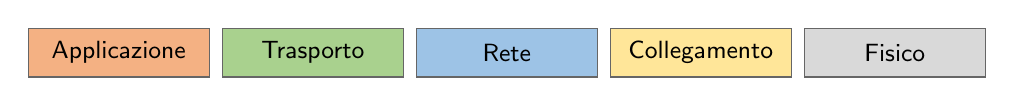
\begin{tikzpicture}[node distance=0.15cm]
  \node[lay app, minimum width=2.3cm] (a) {Applicazione};
  \node[lay tra, minimum width=2.3cm, right=of a] (t) {Trasporto};
  \node[lay net, minimum width=2.3cm, right=of t] (n) {Rete};
  \node[lay link, minimum width=2.3cm, right=of n] (l) {Collegamento};
  \node[lay phy, minimum width=2.3cm, right=of l] (p) {Fisico};
\end{tikzpicture}
\end{center}

% ══════════════════════════════════════════════════════════════
\section{Testi di riferimento e materiale}
% ══════════════════════════════════════════════════════════════

Il corso fa riferimento principalmente a due testi, entrambi citati nelle lezioni:

\begin{itemize}
    \item \textbf{J.F. Kurose, K.W. Ross}, \emph{Computer Networking: A Top-Down Approach}. È il testo
          che dà l'impostazione top-down del corso e da cui provengono molti esempi su HTTP, TCP e IP.
    \item \textbf{A.S. Tanenbaum, N. Feamster, D.J. Wetherall}, \emph{Computer Networks}. Più prolisso
          ma ricchissimo di esempi, anche non strettamente tecnici; usato soprattutto per la
          classificazione delle reti, il livello di collegamento e la crittografia.
\end{itemize}

Le trasparenze sono in inglese (la terminologia di rete è nata in inglese ed è più semplice
impararla così); in questa dispensa i termini tecnici sono riportati sia in italiano sia in
inglese. Le trasparenze sono un \textbf{supporto} alla lezione, non un sostituto dei libri.

\info{Il laboratorio}{
    Per le esercitazioni viene fornito un \textbf{container Docker} già pronto, con tutto il software
    necessario (compilatore, strumenti di rete, Wireshark). Un container è una sorta di macchina
    virtuale leggera che condivide il kernel con la macchina ospite: se qualcosa si rompe, basta
    buttarlo via e ricrearlo, senza toccare il proprio sistema.
}


  % ------------------------------------------------------------------
  \part{Fondamenti e architettura delle reti}
  % ------------------------------------------------------------------
  \chapter{Reti, topologie e categorie}

Questo primo capitolo è \emph{terminologico}: introduce il vocabolario con cui parleremo per
tutto il resto del corso. Non è difficile, ma non va sottovalutato: termini come \emph{host},
\emph{link}, \emph{throughput}, \emph{commutazione di pacchetto}, \emph{ISP} torneranno in
ogni capitolo, e all'esame vanno usati con precisione.

\begin{center}
\begin{tikzpicture}[node distance=0.25cm]
  \node[lay app, minimum width=3.2cm] (a) {Applicazioni};
  \node[lay tra, minimum width=3.2cm, below=0pt of a] (t) {Trasporto};
  \node[lay net, minimum width=3.2cm, below=0pt of t] (n) {Rete};
  \node[lay link, minimum width=3.2cm, below=0pt of n] (l) {Collegamento e fisico};
  \node[lbl, right=0.4cm of a, anchor=west, text width=8.5cm, align=left] {il Web, la posta, i messaggi: quello che usiamo ogni giorno};
  \node[lbl, right=0.4cm of t, anchor=west, text width=8.5cm, align=left] {come un flusso di byte sopravvive a una rete che perde pezzi};
  \node[lbl, right=0.4cm of n, anchor=west, text width=8.5cm, align=left] {indirizzi, router, scelta del percorso};
  \node[lbl, right=0.4cm of l, anchor=west, text width=8.5cm, align=left] {frame, errori, collisioni e cavi veri};
  \draw[-{Stealth[length=3mm]}, very thick, primary] ([xshift=-0.5cm]a.north west) -- ([xshift=-0.5cm]l.south west);
\end{tikzpicture}
\end{center}

Il corso parte dall'alto (le applicazioni) e scende verso il basso; lungo il percorso si
scrivono programmi in C sui socket, e si chiude con sicurezza e privatezza. Oggi, però, si
risponde a due domande più semplici: \textbf{di cosa è fatta una rete} e \textbf{come si
classificano le reti}.

% ══════════════════════════════════════════════════════════════
\section{Che cos'è una rete di calcolatori}
% ══════════════════════════════════════════════════════════════

\dfn{Rete di calcolatori}{
    Una \textbf{rete di calcolatori} è una collezione di dispositivi di calcolo
    \textbf{interconnessi} e \textbf{autonomi}. Due dispositivi sono interconnessi se possono
    \textbf{scambiarsi informazione}.
}

Le due parole chiave vanno prese sul serio.

\begin{itemize}
    \item \textbf{Autonomi}: nessun dispositivo comanda gli altri. Ognuno ha la propria capacità di
          calcolo e funziona per conto suo: se un nodo si spegne, gli altri continuano a lavorare.
    \item \textbf{Interconnessi}: esiste un mezzo attraverso cui i dispositivi si scambiano bit. Può
          essere rame, fibra ottica o onde radio: alla definizione \emph{non importa}.
\end{itemize}

\begin{esempio}{Autonomo o no?}
Un disco SSD collegato con due metri di cavo USB al vostro portatile \textbf{non} forma una rete
con il portatile: è una periferica, completamente controllata dal calcolatore a cui è attaccata.
Il vostro smartphone e il portatile collegati allo stesso Wi-Fi, invece, sono due dispositivi
autonomi che si scambiano informazione: formano una rete. Anche un piccolo sensore che fa
misure e le trasmette è un dispositivo autonomo. ``Dispositivo di calcolo'' non significa
necessariamente ``computer'' in senso stretto.
\end{esempio}

Le reti, a loro volta, possono essere collegate tra loro formando reti più grandi.
L'esempio per eccellenza è \textbf{Internet}, che è appunto una \emph{rete di reti}.

\info{L'unica trasmissione ``vera'' è quella fisica}{
    Quando scaricate un film da un server, a voi sembra che il vostro programma parli direttamente
    con il programma sul server. In realtà l'informazione viaggia solo come \textbf{fenomeno fisico}
    (impulsi elettrici, luce, onde radio). Tutte le altre ``conversazioni'' tra programmi sono
    \emph{virtuali}: poggiano sulla trasmissione fisica. Questa idea diventerà centrale nel prossimo
    capitolo, con il modello a strati.
}

\subsection{A cosa servono le reti}

Gli usi principali delle reti sono:

\begin{itemize}
    \item \textbf{Accesso all'informazione}: pagine Web, basi di dati remote, file condivisi.
    \item \textbf{Comunicazione tra persone}: posta elettronica, messaggistica, videochiamate, VoIP.
    \item \textbf{Commercio elettronico}: acquisti online, home banking.
    \item \textbf{Intrattenimento}: streaming audio e video, giochi multiutente.
    \item \textbf{Internet of Things (IoT)}: oggetti ``non informatici'' connessi alla rete, come
          elettrodomestici, termostati, tapparelle, sensori, contatori dell'energia.
\end{itemize}

% ══════════════════════════════════════════════════════════════
\section{Client e server}
% ══════════════════════════════════════════════════════════════

Uno dei concetti fondamentali delle reti è la coppia \textbf{client}--\textbf{server}
(cliente e servitore). L'idea è la stessa del bar: il cliente chiede un caffè, il barista
lo serve. Il barista è sempre lì, pronto, e serve tanti clienti uno dopo l'altro.

\dfn{Client e server}{
    Un \textbf{server} è un'entità che \textbf{possiede un'informazione o offre un servizio} e
    resta in attesa di richieste. Un \textbf{client} è un'entità che \textbf{richiede esplicitamente}
    quell'informazione o quel servizio al server. Un singolo server gestisce tipicamente le
    richieste di centinaia o migliaia di client.
}

\begin{figure}[H]
    \centering
    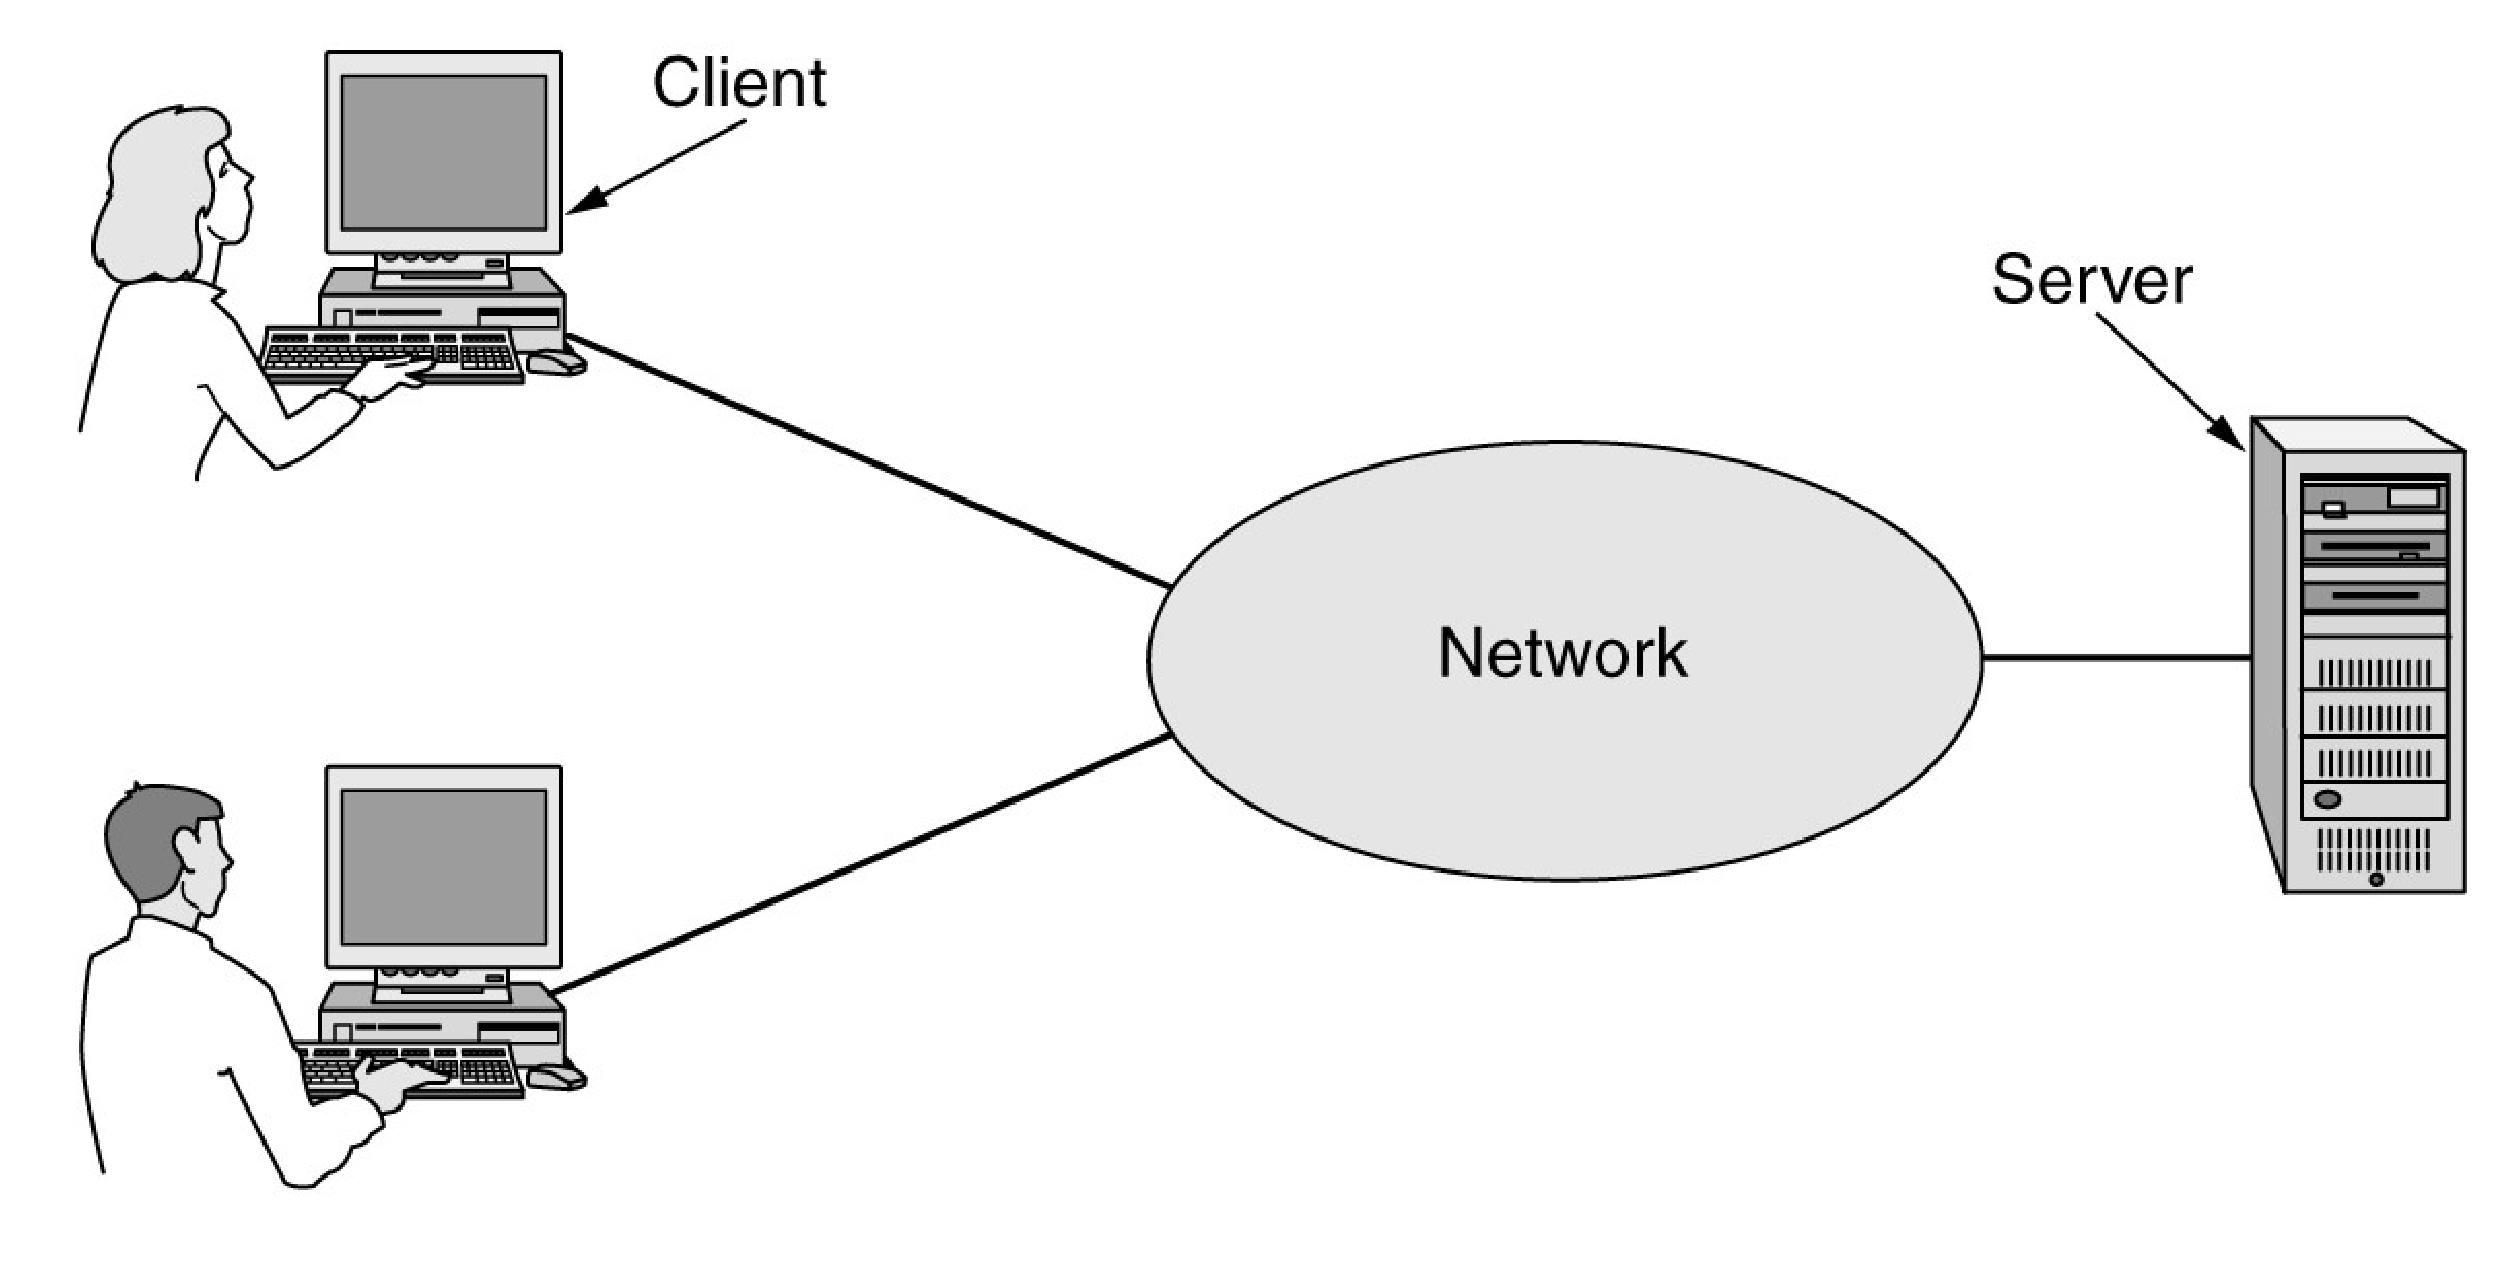
\includegraphics[width=0.55\linewidth]{cap01/client_server.png}
    \caption{Una rete con due client e un server (da Tanenbaum).}
\end{figure}

Esempi che usate già tutti i giorni: il \emph{browser} è un client, il \emph{server Web}
dell'università è un server; il programma di posta sul telefono è un client, il server di
posta di Ateneo, che custodisce la vostra casella e le vostre credenziali, è un server.

\subsection{Client e server sono processi}

Nelle figure disegniamo client e server come macchine, ma chi comunica davvero non è una
macchina: è un \textbf{processo}, cioè un programma in esecuzione su quella macchina.

\begin{figure}[H]
    \centering
    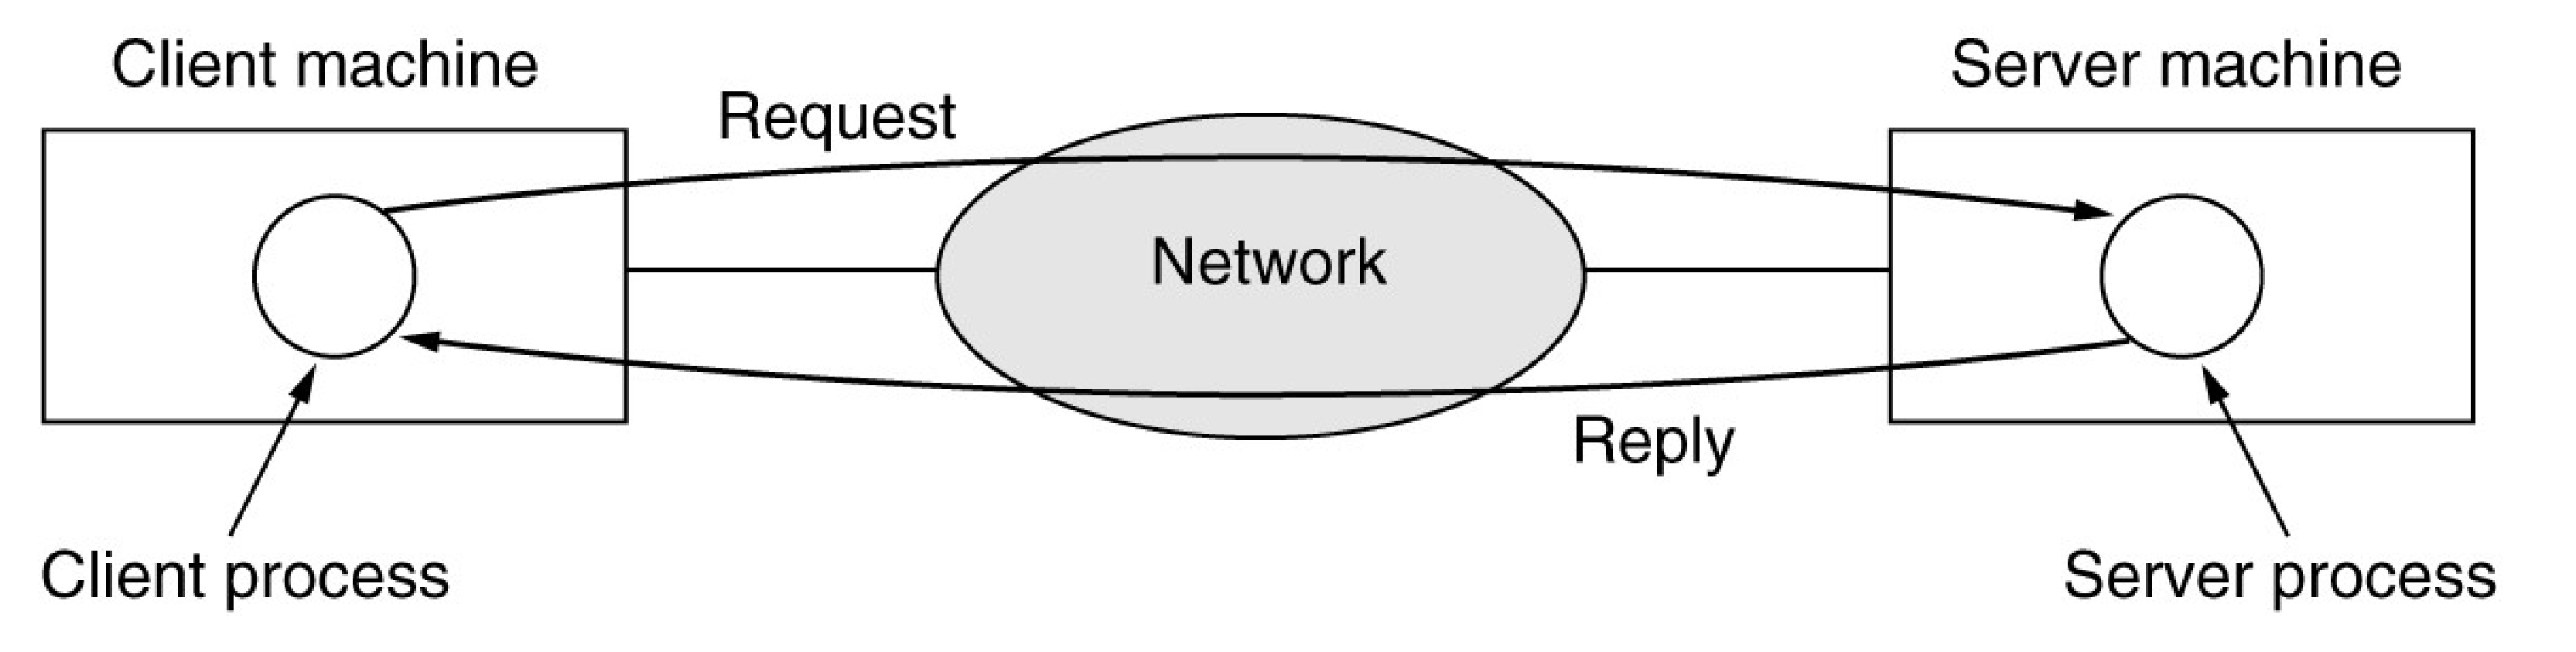
\includegraphics[width=0.75\linewidth]{cap01/client_server_processi.png}
    \caption{La comunicazione avviene tra un processo client e un processo server.}
\end{figure}

Lo schema di interazione è sempre lo stesso: il processo client \textbf{invia un messaggio di
richiesta} e poi \textbf{attende una risposta}; il processo server riceve la richiesta, esegue
un'azione (per esempio legge un file dal disco) e \textbf{invia la risposta}.

\begin{figure}[H]
\centering
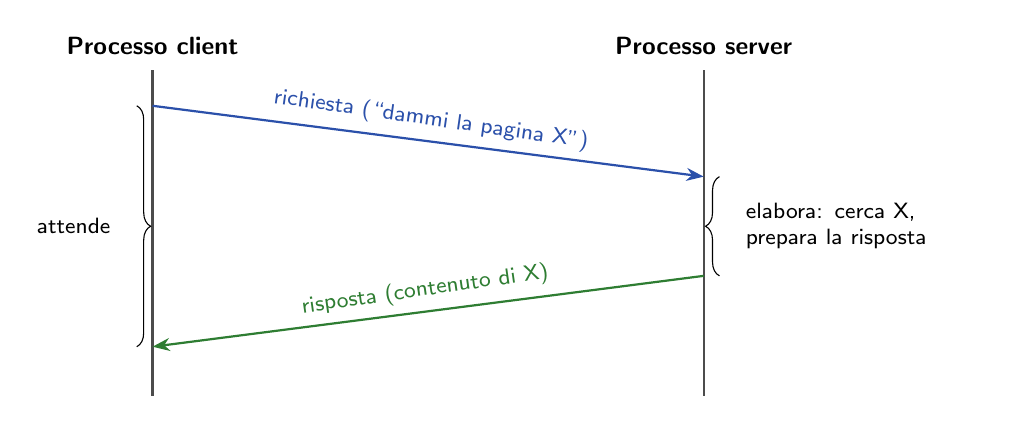
\begin{tikzpicture}[yscale=0.9]
  \timeline{c}{0}{Processo client}{4.6}
  \timeline{s}{7}{Processo server}{4.6}
  \draw[msg, netblue] (0,-0.5) -- node[lbl, above, sloped] {richiesta (``dammi la pagina X'')} (7,-1.5);
  \draw[decorate, decoration={brace, amplitude=5pt, mirror}] (7.2,-1.5) -- (7.2,-2.9) node[midway, right=6pt, lbl, text width=3cm, align=left] {elabora: cerca X,\\ prepara la risposta};
  \draw[msg, netgreen] (7,-2.9) -- node[lbl, above, sloped] {risposta (contenuto di X)} (0,-3.9);
  \draw[decorate, decoration={brace, amplitude=5pt}] (-0.2,-0.5) -- (-0.2,-3.9) node[midway, left=6pt, lbl] {attende};
\end{tikzpicture}
\caption{Lo scambio richiesta--risposta tra due processi. Il tempo scorre verso il basso.}
\end{figure}

\info{La forma di (quasi) tutto ciò che scriveremo}{
    Due processi, uno per parte, che si scambiano messaggi secondo regole concordate: è la forma
    di quasi tutti i programmi che scriveremo in questo corso, a partire da quelli in C con i socket.
}

\subsection{Peer-to-peer: niente ruoli fissi}

L'architettura client-server non è l'unica possibile.

\dfn{Peer-to-peer (P2P)}{
    In un sistema \textbf{peer-to-peer} (da pari a pari) non esistono client e server fissi: ogni
    partecipante (\emph{peer}) può agire \textbf{sia da client sia da server}. Non esiste un database
    centrale di ciò che è disponibile: ogni peer chiede ai peer che conosce.
}

\begin{figure}[H]
    \centering
    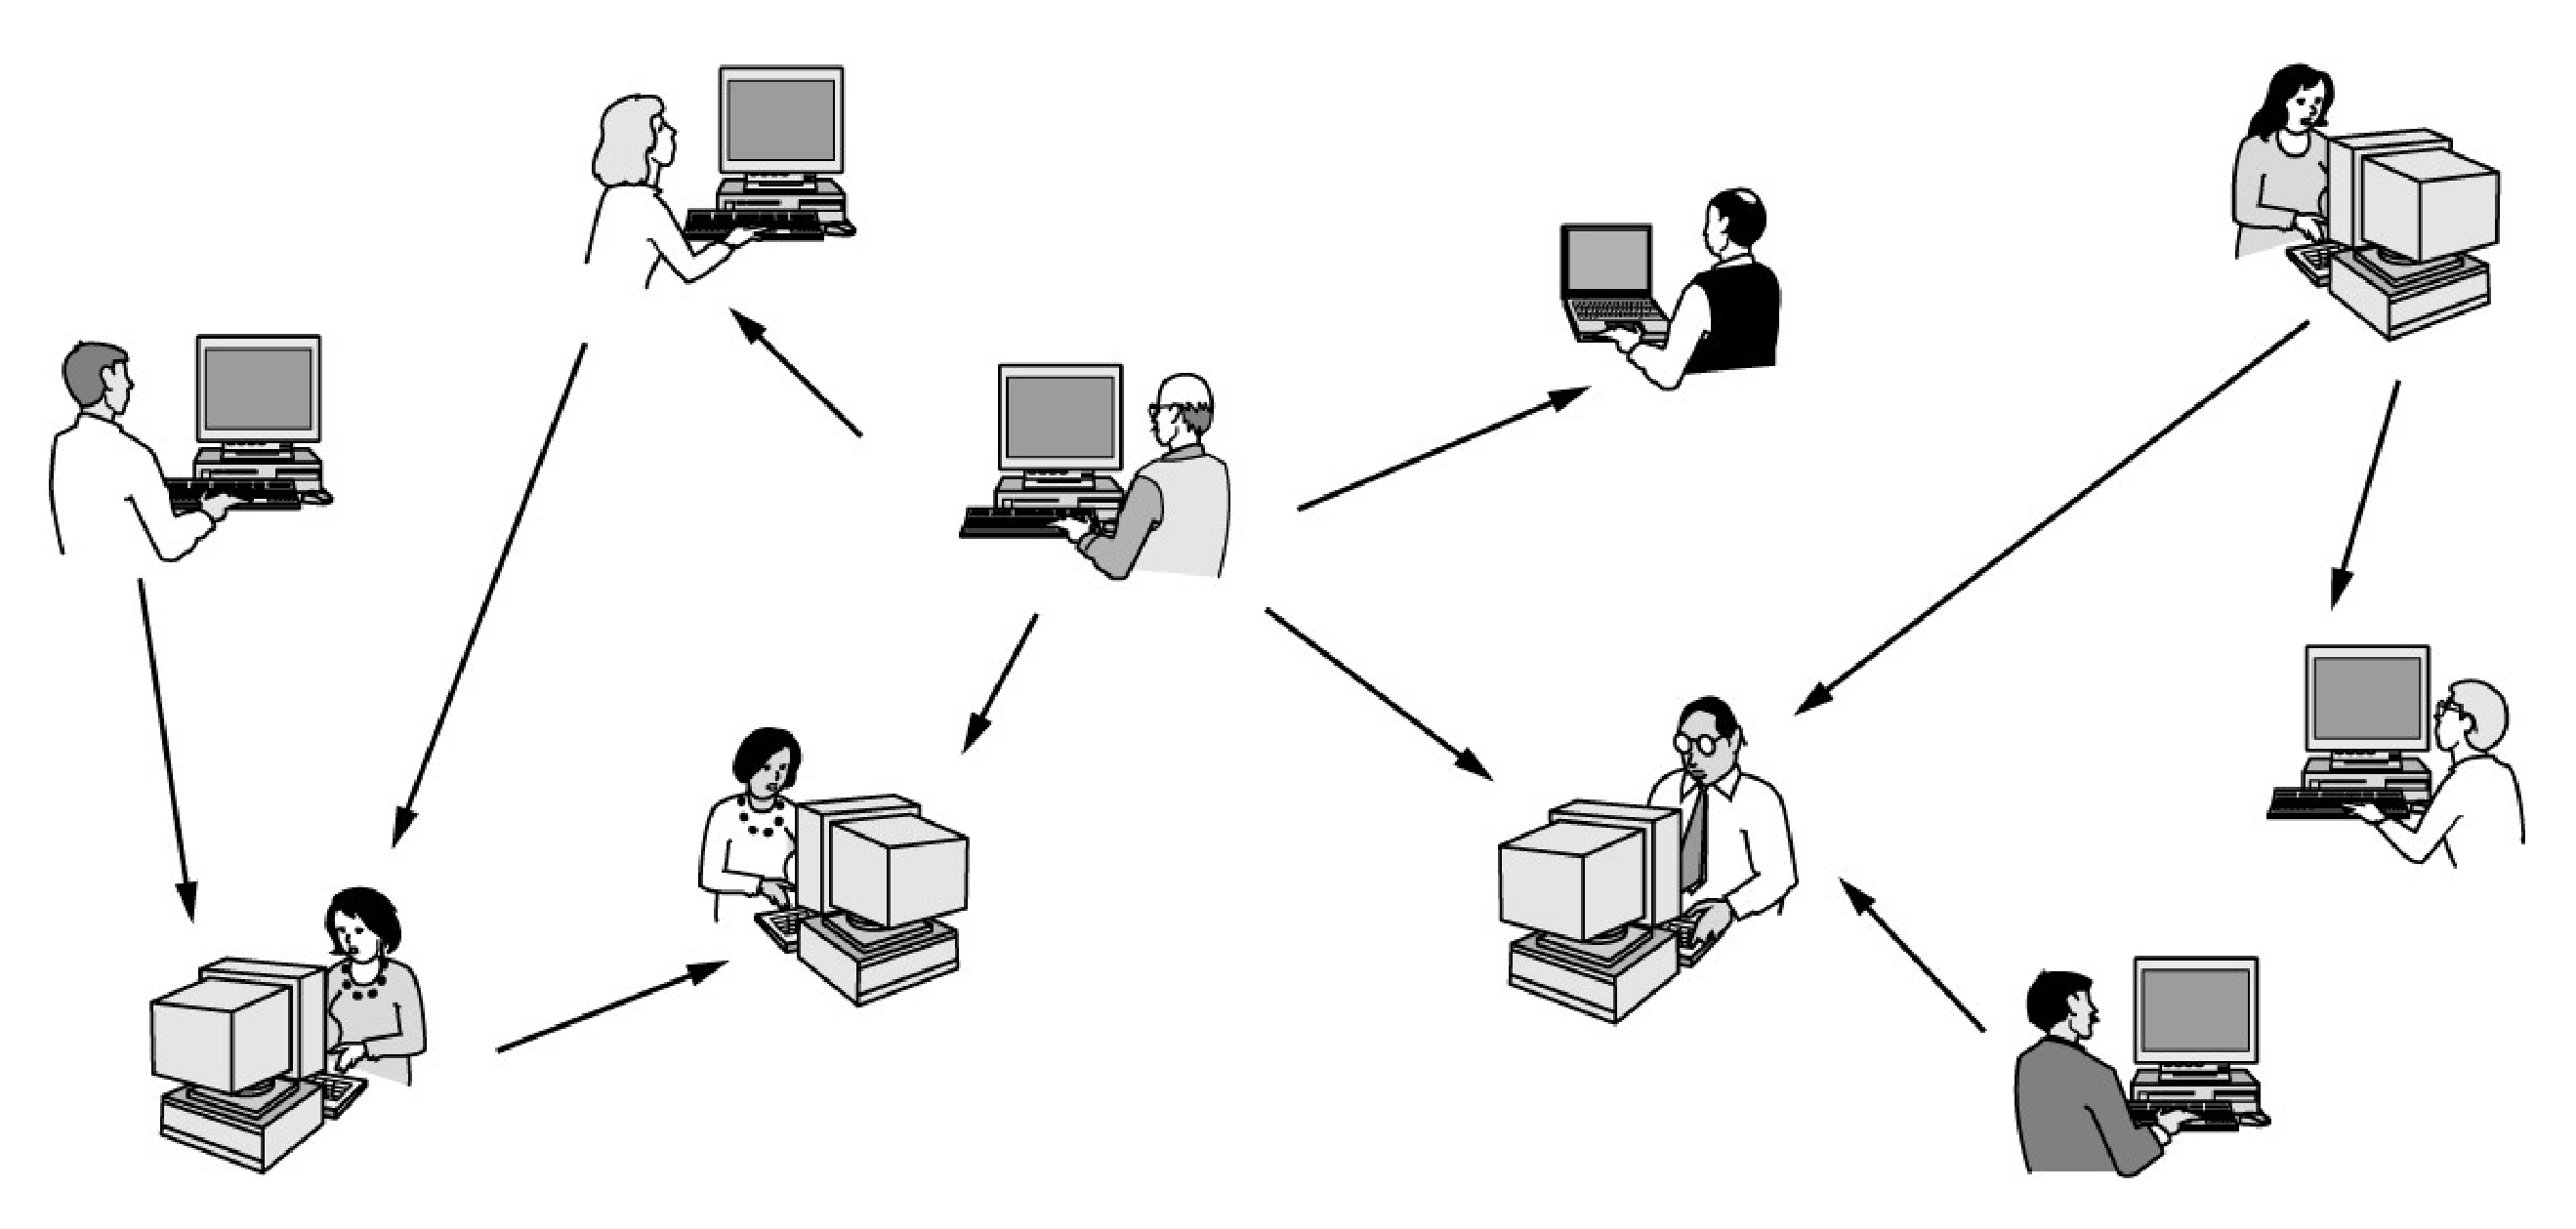
\includegraphics[width=0.6\linewidth]{cap01/p2p.png}
    \caption{In un sistema peer-to-peer ogni nodo può chiedere e fornire servizi.}
\end{figure}

Poiché non c'è un elenco centrale, i protocolli P2P devono prevedere dei meccanismi per
\textbf{scoprire} gli altri partecipanti e ciò che offrono. In cambio, il carico è distribuito:
ogni peer che scarica un file può anche ridistribuirlo ad altri (lo vedremo con BitTorrent).

\begin{table}[H]
\centering
\begin{tabular}{p{3.2cm}p{5.6cm}p{5.6cm}}
\toprule
 & \textbf{Client-server} & \textbf{Peer-to-peer} \\
\midrule
Ruoli & fissi: chi chiede e chi serve & ogni peer fa entrambe le cose \\
Punto centrale & il server (sempre acceso, indirizzo noto) & nessuno, o solo di supporto \\
Scalabilità & il server deve reggere tutti i client & ogni nuovo peer aggiunge capacità \\
Problemi tipici & costo e guasto del server & scoperta dei peer, sicurezza, affidabilità \\
Esempi & Web, posta elettronica & BitTorrent, alcune parti di VoIP \\
\bottomrule
\end{tabular}
\caption{Confronto tra le due architetture.}
\end{table}

% ══════════════════════════════════════════════════════════════
\section{Internet: una rete di reti}
% ══════════════════════════════════════════════════════════════

Anche se la usiamo tutti i giorni, non è affatto ovvio che cosa sia Internet.

\dfn{Internet}{
    \textbf{Internet} è una \textbf{rete di reti} (\emph{internetwork}): un insieme di reti
    \textbf{indipendenti}, con tecnologie diverse e gestite da organizzazioni diverse, collegate tra
    loro attraverso i \textbf{fornitori di accesso} (ISP) in modo da comportarsi come
    \textbf{un'unica rete}. Il nome stesso lo dice: \emph{inter-net}, rete tra reti.
}

\begin{figure}[H]
    \centering
    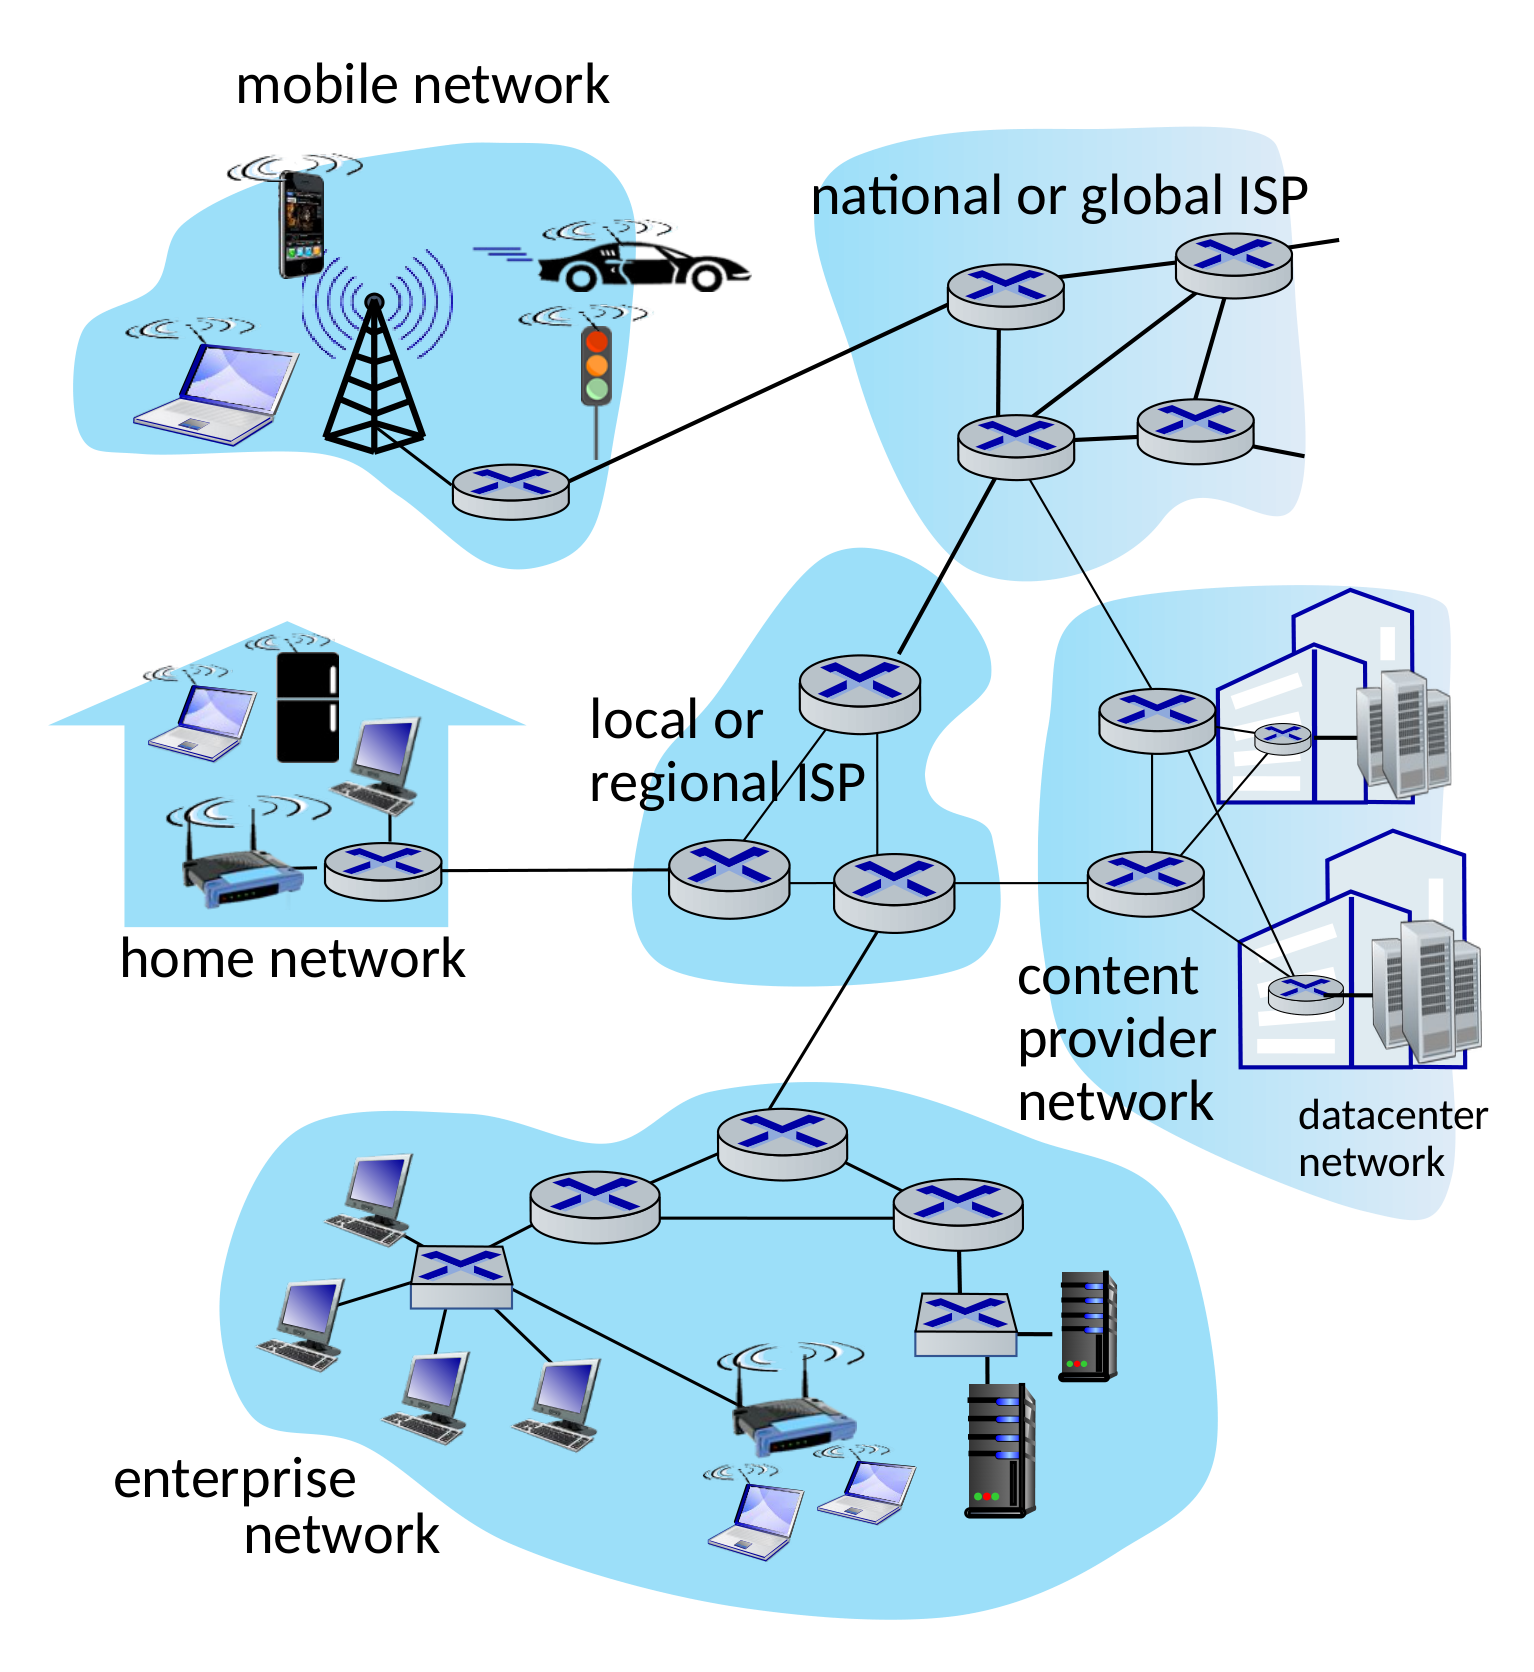
\includegraphics[width=0.62\linewidth]{cap01/internet_rete_di_reti.png}
    \caption{Reti domestiche, aziendali, mobili e di data center, collegate attraverso gli ISP (da Kurose).}
\end{figure}

Guardiamo la figura partendo da casa nostra:

\begin{itemize}
    \item La \textbf{rete di casa} (\emph{home network}) collega telefoni, portatili, stampante,
          televisore. È gestita dal \textbf{router di casa}, in modo indipendente: il vostro
          fornitore di accesso non sa e non si occupa di come sono organizzati i dispositivi dentro
          casa vostra.
    \item Il router di casa si collega alla rete di un \textbf{ISP locale o regionale}, quello a cui
          pagate l'abbonamento.
    \item Allo stesso modo, la \textbf{rete aziendale} (\emph{enterprise network}, per esempio la
          rete dell'Università) e la \textbf{rete mobile} del vostro operatore telefonico sono reti
          a sé, ciascuna con la propria gestione.
    \item Gli ISP locali e regionali sono a loro volta collegati a \textbf{ISP nazionali o globali},
          che trasportano il traffico tra regioni e continenti.
    \item Accanto a loro ci sono le reti dei \textbf{content provider} e dei \textbf{data center}
          (Google, Netflix, \dots), che ospitano i servizi che usiamo.
\end{itemize}

Ogni rete è gestita e integrata nella rete dell'ISP a cui si appoggia; gli ISP sono integrati
in ISP più grandi, e così via, fino a formare un'unica struttura: Internet.

\begin{figure}[H]
\centering
\begin{tikzpicture}[
    every node/.style={font=\footnotesize\sffamily},
    isp/.style={ellipse, draw=netblue!70, fill=cloudbg, minimum width=2.6cm, minimum height=0.9cm, align=center},
    lan/.style={rounded corners=3pt, draw=netgreen!70!black, fill=netgreen!12, minimum width=2.3cm, minimum height=0.9cm, align=center}]
  \node[isp, fill=netblue!25, minimum width=6.5cm] (glob) at (0,0) {ISP nazionali / globali\\(dorsali, backbone)};
  \node[isp] (reg1) at (-3.8,-1.8) {ISP regionale};
  \node[isp] (reg2) at (3.8,-1.8) {ISP regionale};
  \node[isp] (acc1) at (-5.2,-3.6) {ISP di accesso};
  \node[isp] (acc2) at (-1.8,-3.6) {ISP di accesso};
  \node[isp] (mob) at (1.9,-3.6) {operatore\\mobile};
  \node[isp] (acc3) at (5.3,-3.6) {ISP di accesso};
  \node[lan] (home) at (-5.8,-5.4) {\icon[0.45cm]{laptop}\icon[0.3cm]{smartphone}\\rete di casa};
  \node[lan] (home2) at (-3.3,-5.4) {\icon[0.45cm]{pc}\icon[0.45cm]{laptop}\\rete di casa};
  \node[lan] (ent) at (-0.6,-5.4) {\icon[0.45cm]{pc}\icon[0.3cm]{server}\\rete aziendale};
  \node[lan] (phones) at (2.1,-5.4) {\icon[0.3cm]{smartphone}\icon[0.3cm]{smartphone}\\telefoni};
  \node[lan] (dc) at (5.3,-5.4) {\icon[0.3cm]{server}\icon[0.3cm]{server}\\data center};
  \foreach \a/\b in {glob/reg1, glob/reg2, reg1/acc1, reg1/acc2, reg2/mob, reg2/acc3, acc1/home, acc1/home2, acc2/ent, mob/phones, acc3/dc}
     \draw[wired] (\a) -- (\b);
  \draw[wired, dashed, netorange] (dc.north east) to[out=70, in=0] node[pos=0.55, right, lbl, text=netorange] {peering diretto\\del content provider} (glob.east);
  \node[lbl, text=primary] at (0,0.95) {\bfseries Internet = l'insieme di tutte queste reti interconnesse};
\end{tikzpicture}
\caption{Ogni rete si appoggia a un ISP, e gli ISP si appoggiano a ISP più grandi: il risultato è una rete di reti.}
\end{figure}

La cosa straordinaria è che, nonostante tecnologie, velocità, protocolli e contratti diversi,
tutto \emph{funziona come se fossimo sulla stessa rete}. Potete chiamare un parente in Nuova
Zelanda: i vostri dati attraversano decine di reti diverse, ma l'applicazione non se ne accorge.
Non è magia, è un'abilissima progettazione dei protocolli.

\subsection{Il collante: l'Internet Protocol (IP)}

Il protocollo che rende uniforme questa enorme eterogeneità è l'\textbf{Internet Protocol (IP)}.

\dfn{Internet Protocol (IP)}{
    L'\textbf{Internet Protocol} è il protocollo che permette di consegnare pacchetti di dati
    (\textbf{datagrammi}) da un host sorgente a un host destinazione attraverso una rete di reti.
    Ogni interfaccia collegata a Internet ha un \textbf{indirizzo IP}, e ogni datagramma porta con
    sé l'indirizzo del mittente e quello del destinatario. I router leggono l'indirizzo di
    destinazione e inoltrano il datagramma, salto dopo salto, verso la rete giusta.
}

Tre caratteristiche di IP da ricordare fin da ora:

\begin{itemize}
    \item \textbf{È comune a tutti}: qualunque tecnologia ci sia sotto (Ethernet, Wi-Fi, fibra, 4G/5G)
          e qualunque applicazione ci sia sopra (Web, posta, videochiamate), in mezzo c'è sempre IP.
          È l'unico punto su cui tutti devono essere d'accordo.
    \item \textbf{Nasconde le differenze}: le applicazioni vedono un'unica rete, non le decine di reti
          attraversate.
    \item \textbf{È ``best effort''}: IP fa del suo meglio per consegnare i datagrammi, ma non
          garantisce né che arrivino, né che arrivino in ordine. Le garanzie, quando servono, vengono
          aggiunte sopra (da TCP, come vedremo).
\end{itemize}

\begin{figure}[H]
\centering
\begin{tikzpicture}[every node/.style={font=\footnotesize\sffamily}]
  \fill[lapp!70] (-5,2.6) -- (5,2.6) -- (3.2,1.4) -- (-3.2,1.4) -- cycle;
  \node at (0,2.05) {Web \quad posta \quad DNS \quad streaming \quad VoIP \quad giochi \quad \dots};
  \fill[ltra] (-3.2,1.4) -- (3.2,1.4) -- (1.6,0.6) -- (-1.6,0.6) -- cycle;
  \node at (0,1.0) {TCP \quad UDP};
  \fill[lnet] (-1.6,0.6) rectangle (1.6,-0.2);
  \node at (0,0.2) {\bfseries IP};
  \fill[llink] (-1.6,-0.2) -- (1.6,-0.2) -- (3.2,-1.0) -- (-3.2,-1.0) -- cycle;
  \node at (0,-0.6) {Ethernet \quad Wi-Fi \quad 4G/5G};
  \fill[lphy] (-3.2,-1.0) -- (3.2,-1.0) -- (5,-2.2) -- (-5,-2.2) -- cycle;
  \node at (0,-1.6) {rame \quad fibra \quad radio \quad satellite \quad \dots};
  \draw[<-, thick, primary] (1.8,0.2) -- (5.2,0.2) node[right, lbl, text=primary, align=left] {la ``vita stretta''\\della clessidra};
\end{tikzpicture}
\caption{La clessidra di Internet: tante applicazioni sopra, tante tecnologie sotto, un solo protocollo in mezzo.}
\end{figure}

Studieremo IP in dettaglio nella Parte IV; per ora basta sapere che è lui a tenere insieme Internet.

% ══════════════════════════════════════════════════════════════
\section{Breve storia di Internet}
% ══════════════════════════════════════════════════════════════

L'idea di una rete ``universale'' fu teorizzata da alcuni ricercatori (il più noto è
J.C.R.~Licklider) già negli anni '50--'60. Le tappe da ricordare sono poche.

\begin{figure}[H]
\centering
\begin{tikzpicture}[every node/.style={font=\footnotesize\sffamily}]
  \draw[-{Stealth[length=3mm]}, line width=2pt, primary] (0,0) -- (15.5,0);
  \foreach \x/\y/\t/\d in {0.8/1969/ARPANET/{4 nodi: UCLA, SRI,\\UCSB, Utah}, 4.0/1974/TCP e IP/{Kahn e Cerf\\progettano TCP/IP}, 7.2/1986/NSFNET/{dorsale TCP/IP\\per la ricerca}, 10.4/1990/fine ARPANET/{ARPANET viene\\dismessa}, 13.6/1995/fine NSFNET/{cadono le ultime\\restrizioni commerciali}} {
    \fill[primary] (\x,0) circle (4pt);
    \node[above=6pt, font=\bfseries\sffamily] at (\x,0) {\y};
    \node[above=20pt, text=primary!80!black] at (\x,0) {\t};
    \node[below=6pt, align=center] at (\x,0) {\d};
  }
\end{tikzpicture}
\caption{Le tappe principali: da rete di ricerca a Internet commerciale.}
\end{figure}

\begin{itemize}
    \item \textbf{1969 --- ARPANET}. L'agenzia ARPA del Dipartimento della Difesa statunitense finanzia
          una rete di ricerca per università e centri di ricerca. Alla fine del 1969 ha quattro nodi:
          UCLA, SRI (Stanford Research Institute), UC Santa Barbara e Utah. Reti simili nascevano in modo
          indipendente negli USA e in Europa.
    \item \textbf{1974 --- TCP/IP}. Robert Kahn e Vinton Cerf progettano il \emph{Transmission Control
          Protocol} (TCP) e l'\emph{Internet Protocol} (IP), i protocolli su cui poggia ancora oggi Internet.
    \item \textbf{1986 --- NSFNET}. La National Science Foundation finanzia una dorsale basata su TCP/IP.
          Si va verso l'idea di rete di reti, ma sia ARPANET sia NSFNET vietano il traffico commerciale.
    \item \textbf{1990} --- ARPANET viene dismessa.
    \item \textbf{1995} --- anche NSFNET viene dismessa e con lei cade l'ultima restrizione al traffico
          commerciale: nella seconda metà degli anni '90 nasce l'Internet che usiamo.
\end{itemize}

\begin{figure}[H]
    \centering
    \begin{minipage}{0.45\linewidth}\centering
      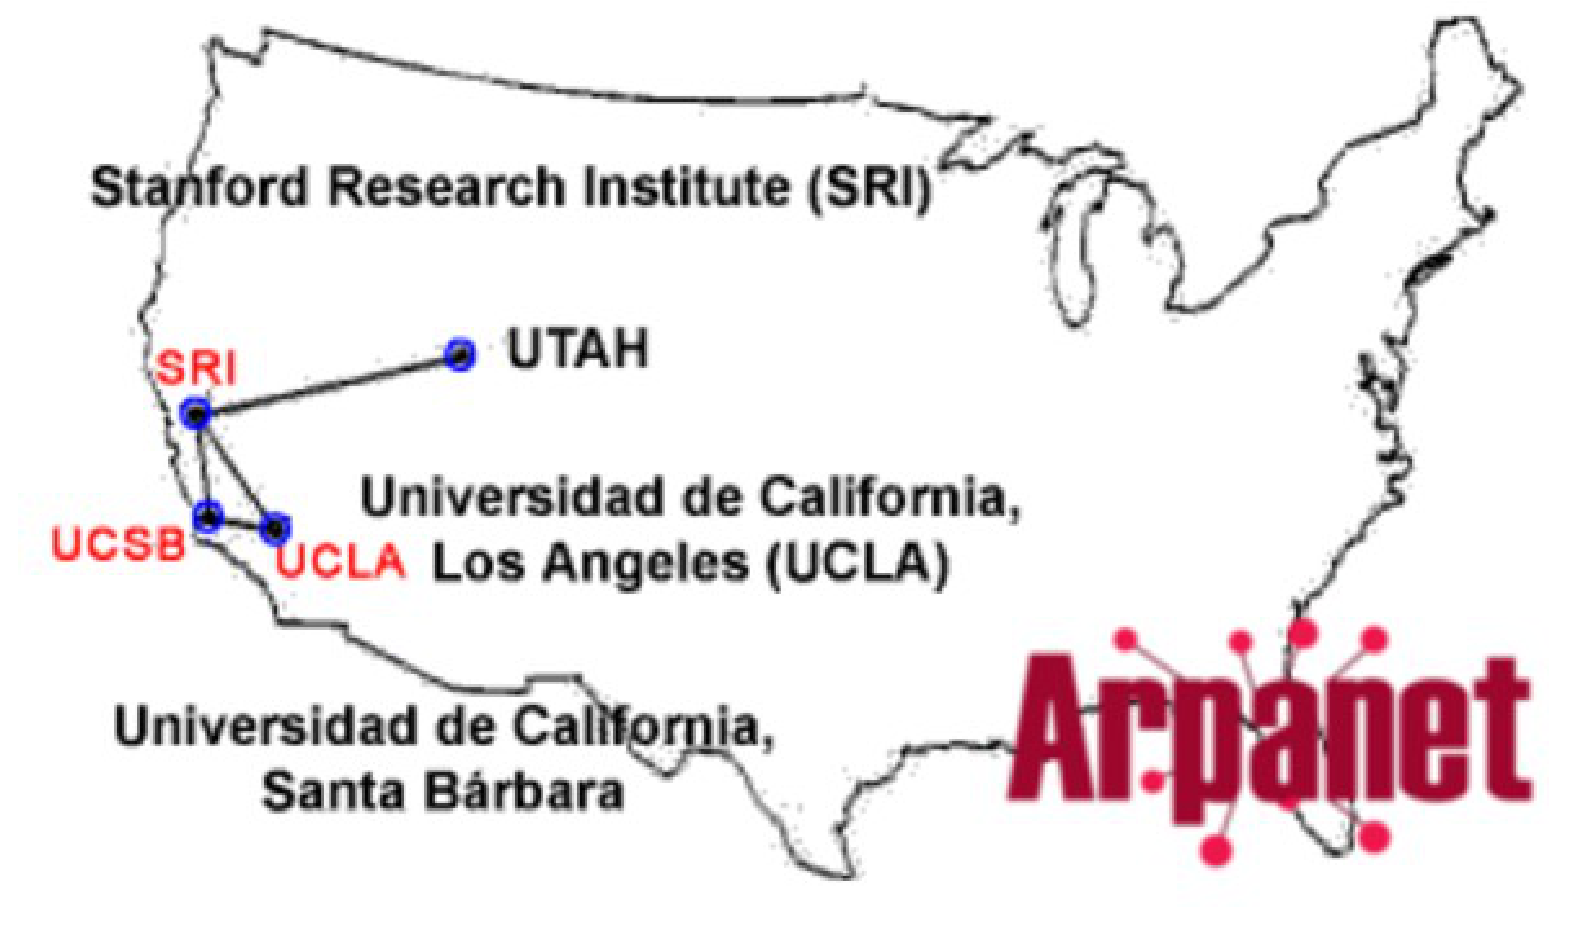
\includegraphics[width=\linewidth]{cap01/arpanet_1969.png}\\
      {\small (a) ARPANET nel 1969}
    \end{minipage}\hfill
    \begin{minipage}{0.45\linewidth}\centering
      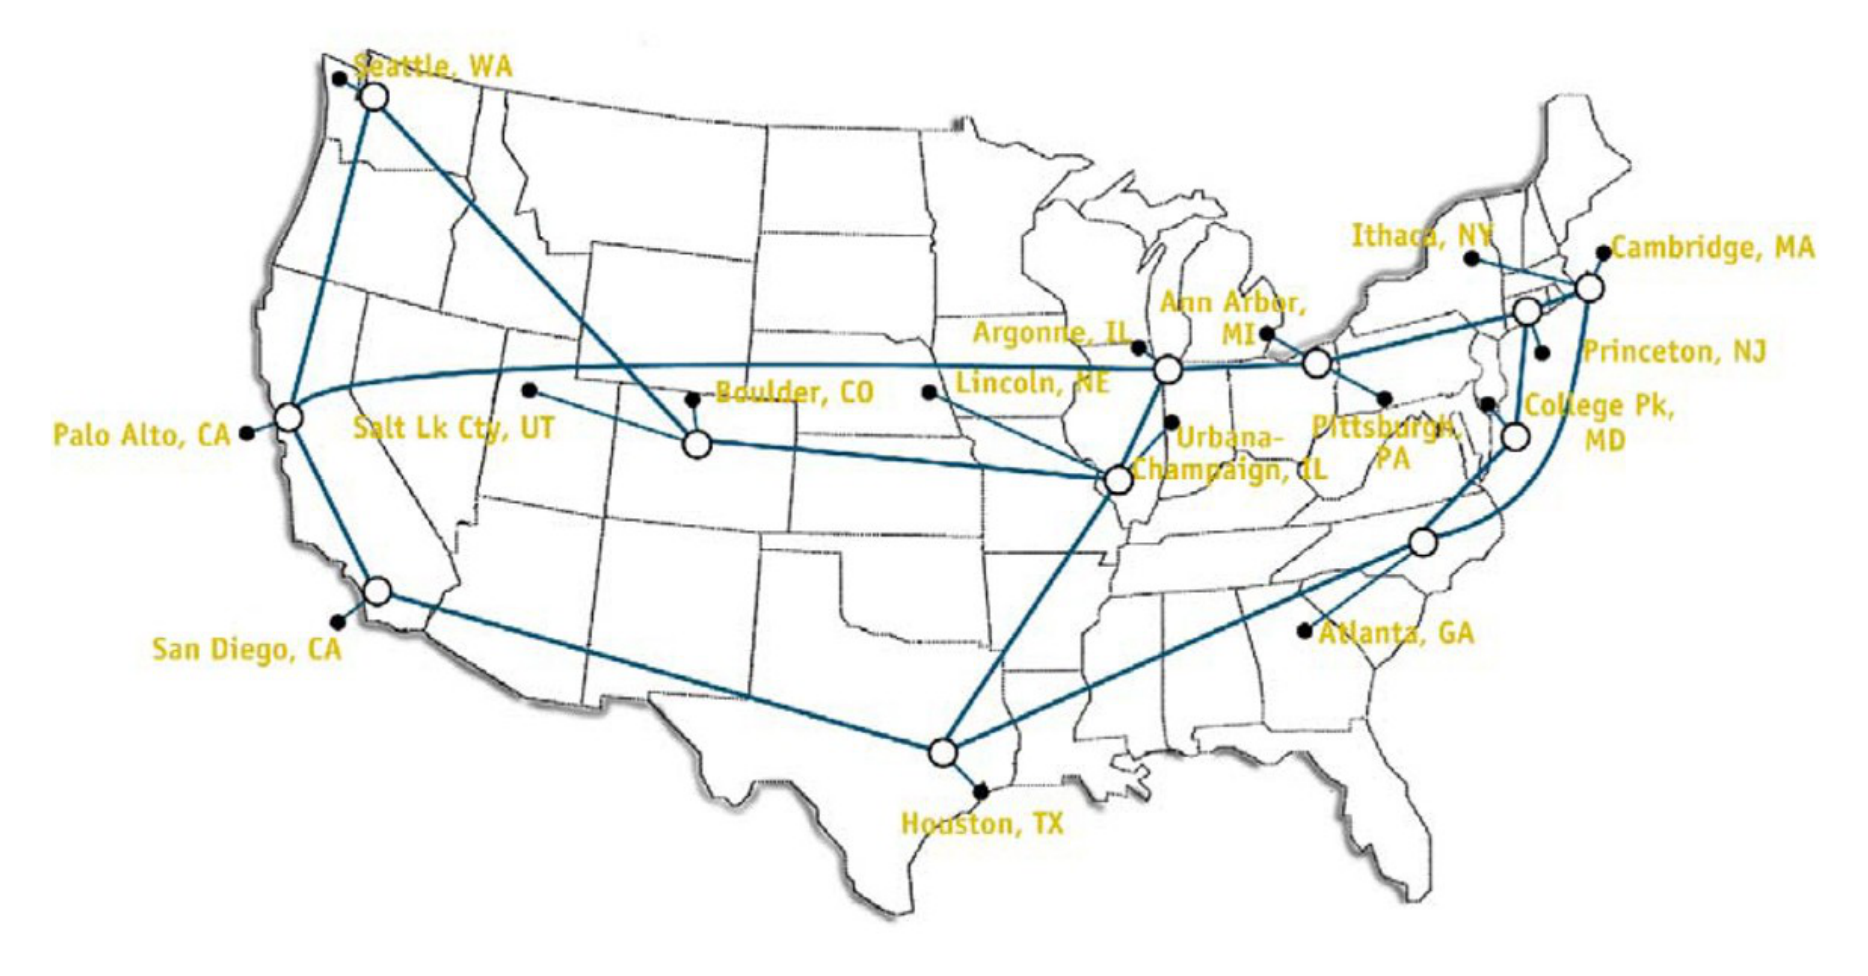
\includegraphics[width=\linewidth]{cap01/nsfnet_1992.png}\\
      {\small (b) la dorsale NSFNET nel 1992}
    \end{minipage}
    \caption{Due fotografie della rete prima dell'Internet commerciale.}
\end{figure}

\info{Perché la storia conta}{
    Internet non è stata progettata come un sistema unico e coerente: è cresciuta
    \textbf{aggregando reti preesistenti e diverse tra loro}. Per questo i suoi protocolli sono
    progettati per tollerare l'eterogeneità. Prima di Internet esistevano reti non integrate tra loro
    (per esempio il Minitel francese), lente e poco pervasive, che non ebbero lo stesso impatto.
}

% ══════════════════════════════════════════════════════════════
\section{Di cosa è fatta una rete: dispositivi, collegamenti, host}
% ══════════════════════════════════════════════════════════════

Fisicamente, una rete è composta da due grandi famiglie di elementi.

\dfn{Infrastruttura e host}{
    \begin{itemize}
      \item L'\textbf{infrastruttura} è l'insieme dei \textbf{dispositivi di rete} e dei
            \textbf{collegamenti} (\emph{link}) tra loro. È dedicata esclusivamente a far comunicare i
            dispositivi, non a eseguire applicazioni per gli utenti.
      \item Gli \textbf{host}, detti anche \textbf{sistemi terminali} (\emph{end systems}), sono le
            macchine che \textbf{eseguono le applicazioni} e che producono o consumano i dati.
    \end{itemize}
}

\subsection{I dispositivi dell'infrastruttura}

Nelle figure di rete si usano dei simboli standard, in larga parte introdotti da Cisco, per
indicare i dispositivi. Conviene impararli subito.

\begin{table}[H]
\centering
\begin{tabular}{>{\centering\arraybackslash}m{2cm} m{2.3cm} m{10cm}}
\toprule
\textbf{Simbolo} & \textbf{Dispositivo} & \textbf{Che cosa fa} \\
\midrule
\icon[1.3cm]{router} & \textbf{Router} & Collega \textbf{reti diverse} e inoltra i pacchetti verso la rete
di destinazione, scegliendo ogni volta da quale collegamento farli uscire (in base all'indirizzo IP).
È il dispositivo che tiene insieme Internet. \\
\icon[1.1cm]{accesspoint} & \textbf{Access point} & Punto di accesso \textbf{senza fili}: collega i
dispositivi Wi-Fi alla rete cablata, facendo da ``ponte'' tra le onde radio e il cavo. \\
\icon[1.2cm]{switch} & \textbf{Switch} & Collega più dispositivi \textbf{della stessa rete locale}.
Riceve un frame su una porta e lo inoltra \textbf{solo} sulla porta a cui è collegato il destinatario
(in base all'indirizzo fisico, detto MAC). \\
\icon[1.2cm]{hub} & \textbf{Hub} & Il ``fratello povero'' dello switch: tutto ciò che riceve su una
porta lo \textbf{ripete su tutte le altre}, senza guardare a chi è destinato. Oggi è quasi del tutto
sostituito dagli switch. \\
\bottomrule
\end{tabular}
\caption{I principali dispositivi di rete e i loro simboli.}
\end{table}

\info{Il router di casa fa tante cose insieme}{
    Il ``router'' che l'operatore vi installa in casa è in realtà un apparecchio che contiene
    \emph{più} dispositivi: un router (verso l'ISP), uno switch (le porte Ethernet sul retro), un
    access point (il Wi-Fi) e spesso anche il modem. Nelle figure li disegneremo separati.
}

\subsection{Gli host}

\begin{center}
\begin{tabular}{cccc}
\icon[1.4cm]{laptop} & \icon[0.8cm]{server} & \icon[1.3cm]{smartphone} & \icon[1.1cm]{pc} \\
\small Laptop & \small Server & \small Smartphone & \small PC
\end{tabular}
\end{center}

Sono host il portatile, lo smartphone, il PC, il server del sistema informativo di Ateneo, il
Raspberry che a casa fa da server per i file: tutte macchine che \textbf{eseguono applicazioni}.

\dfn{Commutatore di pacchetto (packet switch)}{
    Router e switch sono entrambi \textbf{commutatori di pacchetto}: \textbf{ricevono} un pacchetto di
    dati da un collegamento e lo \textbf{inoltrano} su un altro collegamento.
}

\warning{Nodo non vuol dire host}{
    Un router è un \textbf{nodo} della rete ma \textbf{non è un host}: non esegue applicazioni per gli
    utenti. Come vedremo nel prossimo capitolo, non implementa nemmeno tutti gli strati della pila
    protocollare.
}

\subsection{La rete come grafo}

Le reti condividono il vocabolario con la \textbf{teoria dei grafi}.

\dfn{Nodi, collegamenti e cammini}{
    I dispositivi connessi alla rete sono i \textbf{nodi}; le connessioni tra nodi sono i
    \textbf{collegamenti} (\emph{link}, o canali di comunicazione). Una sequenza di nodi e collegamenti
    che porta da un estremo all'altro è un \textbf{cammino} (\emph{path}). Gli \textbf{host} sono i nodi
    speciali che forniscono o usano servizi.
}

\begin{figure}[H]
    \centering
    \begin{minipage}{0.47\linewidth}\centering
      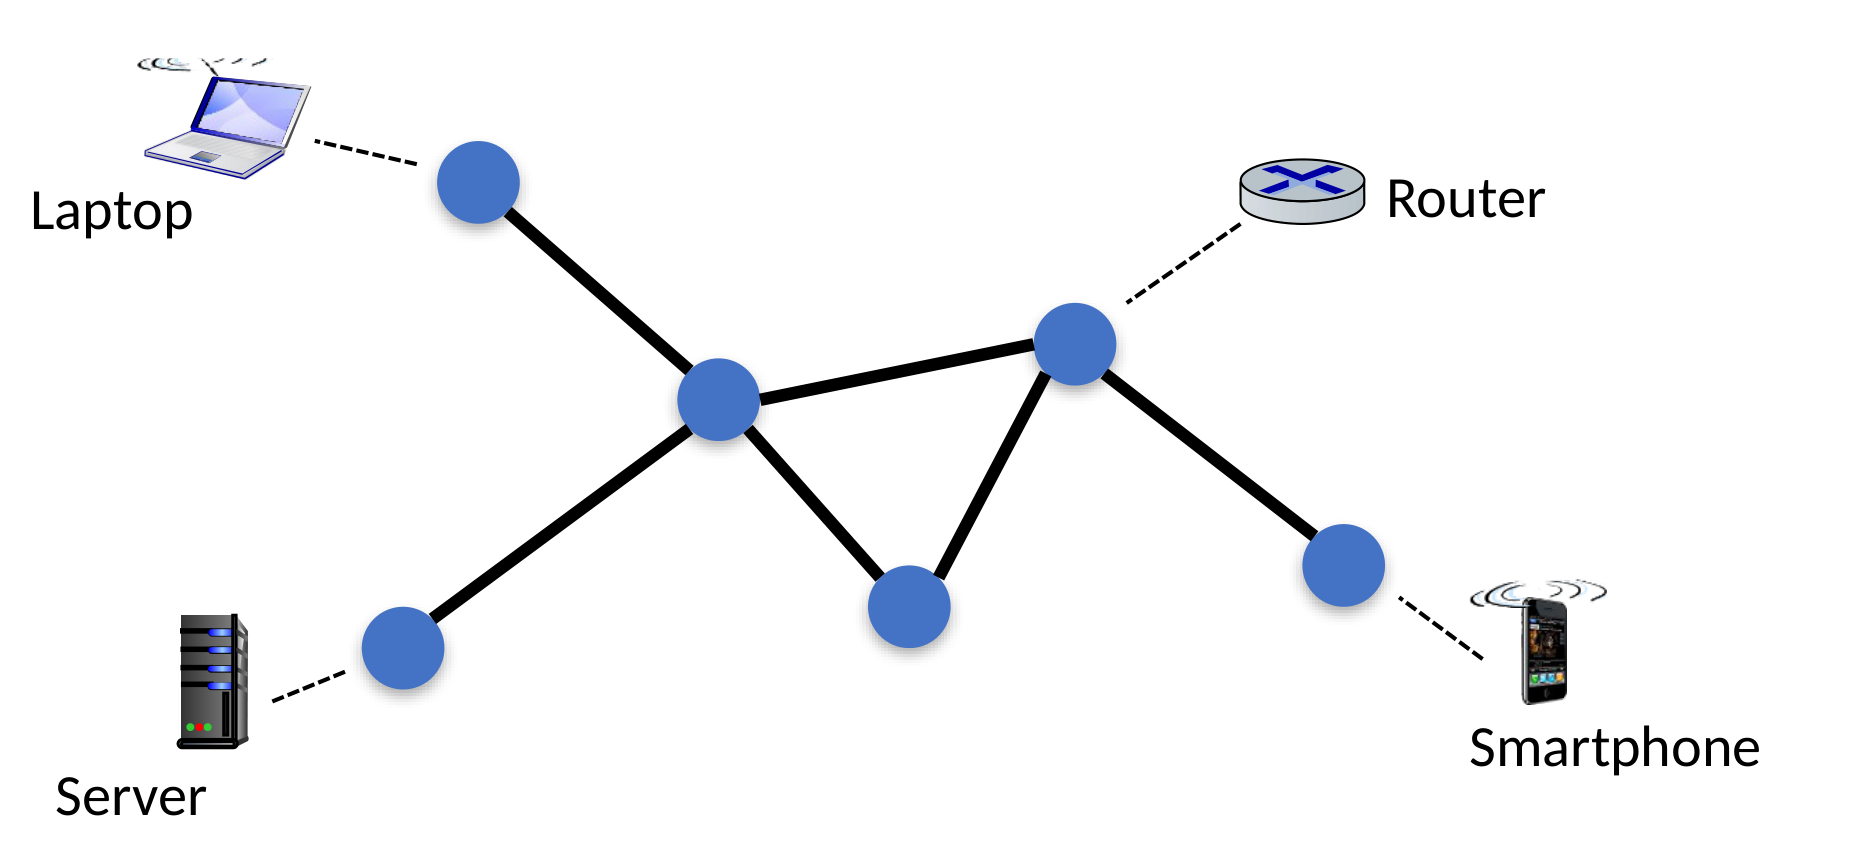
\includegraphics[width=\linewidth]{cap01/rete_grafo.png}\\ {\small (a) la rete come grafo}
    \end{minipage}\hfill
    \begin{minipage}{0.47\linewidth}\centering
      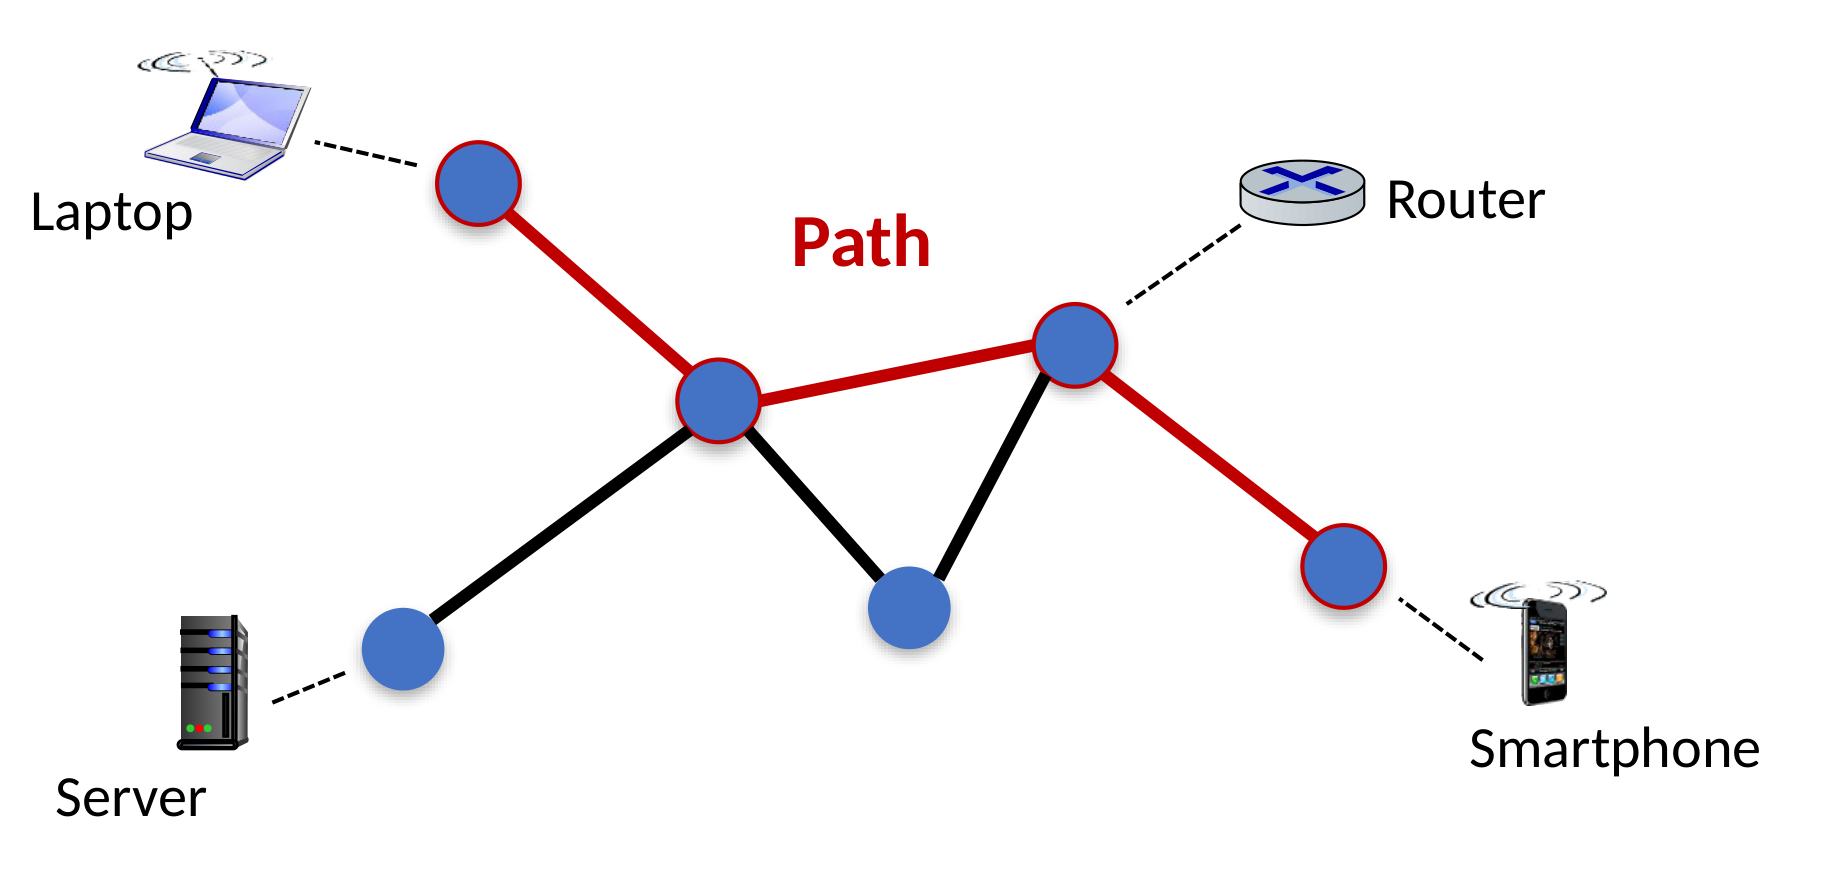
\includegraphics[width=\linewidth]{cap01/rete_path.png}\\ {\small (b) un cammino tra due host}
    \end{minipage}
    \caption{Idealmente gli host sono le foglie del grafo e i nodi intermedi inoltrano i dati.}
\end{figure}

Idealmente gli host stanno sulle \textbf{foglie} del grafo, mentre i nodi intermedi (router,
switch) si occupano di inoltrare i dati (nella pratica non sempre è così). Se telefonate a un
parente in Nuova Zelanda non esiste un cavo diretto tra i due telefoni: i dati seguono un
cammino attraverso molti nodi. A meno di stendere un cavo dedicato, cosa che alcune
organizzazioni con esigenze di sicurezza o affidabilità fanno davvero.

% ══════════════════════════════════════════════════════════════
\section{Le cinque componenti di una comunicazione}
% ══════════════════════════════════════════════════════════════

Ogni comunicazione di dati, qualunque sia la tecnologia usata, ha cinque componenti.

\begin{figure}[H]
\centering
\begin{tikzpicture}[every node/.style={font=\small\sffamily}]
  \node[box, fill=lphy!60, minimum width=2.4cm] (snd) at (0,0) {\icon[0.9cm]{pc}\\Mittente};
  \node[box, fill=lphy!60, minimum width=2.4cm] (rcv) at (10,0) {\icon[0.9cm]{laptop}\\Destinatario};
  \draw[line width=2.5pt, netred] (snd.east) -- (rcv.west) node[midway, below=4pt, text=netred] {Mezzo trasmissivo};
  \node[box, fill=yellow!60, minimum width=2cm] (m) at (5,1.3) {Messaggio};
  \draw[msg, netred] (m.east) -- ++(1.2,0);
  \node[box, fill=cloudbg, text width=2.2cm, align=left, font=\scriptsize\sffamily] (p1) at (0,2.4) {Regola 1: \dots\\Regola 2: \dots\\Regola $n$: \dots};
  \node[box, fill=cloudbg, text width=2.2cm, align=left, font=\scriptsize\sffamily] (p2) at (10,2.4) {Regola 1: \dots\\Regola 2: \dots\\Regola $n$: \dots};
  \node[above=1pt of p1] {Protocollo};
  \node[above=1pt of p2] {Protocollo};
  \draw[dashed, thick, primary] (p1.east) -- node[above, lbl, text=primary] {stesse regole da entrambe le parti} (p2.west);
  \foreach \n/\pos in {1/{5,1.95}, 2/{-1.55,-0.6}, 3/{11.55,-0.6}, 4/{5,-0.85}, 5/{11.55,2.9}}
     \node[circle, fill=primary, text=white, font=\scriptsize\bfseries, inner sep=1.5pt] at (\pos) {\n};
\end{tikzpicture}
\caption{Le cinque componenti: (1) messaggio, (2) mittente, (3) destinatario, (4) mezzo, (5) protocollo.}
\end{figure}

\begin{enumerate}
    \item \textbf{Messaggio}: i dati da trasmettere.
    \item \textbf{Mittente} (\emph{sender}): l'entità che invia il messaggio.
    \item \textbf{Destinatario} (\emph{receiver}): l'entità che deve ricevere il messaggio.
    \item \textbf{Mezzo} (\emph{medium}): il canale fisico attraverso cui il messaggio viaggia.
    \item \textbf{Protocollo}: l'insieme di regole, note a entrambi, che fanno funzionare lo scambio.
\end{enumerate}

L'ultima componente è la più importante: senza un protocollo condiviso, i bit che arrivano al
destinatario sono solo rumore.

\subsection{Che cos'è un protocollo}

\dfn{Protocollo}{
    Un \textbf{protocollo} definisce il \textbf{formato} e l'\textbf{ordine} dei messaggi scambiati tra
    due o più entità comunicanti, e le \textbf{azioni} intraprese quando un messaggio viene inviato o
    ricevuto.
}

I protocolli esistono anche nella vita di tutti i giorni. Quando rispondete al telefono dite
``Pronto'' (in un'azienda si risponde con il nome della ditta); chi chiama aspetta che l'altro
parli per primo; mentre uno parla, l'altro non dovrebbe parlare. Chiedere l'ora a uno
sconosciuto ha la stessa struttura: un saluto, un saluto di risposta, poi la domanda vera.

\begin{figure}[H]
\centering
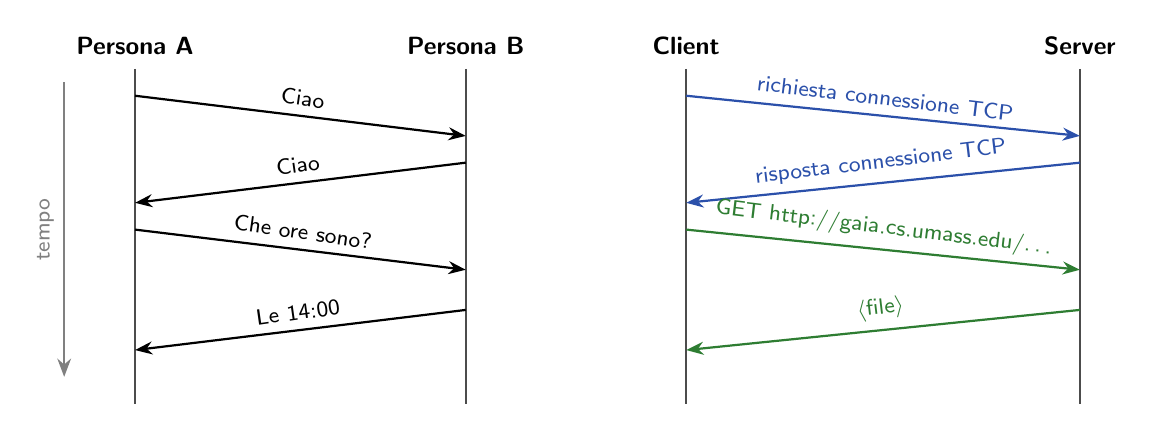
\begin{tikzpicture}[yscale=0.85]
  \begin{scope}
    \timeline{a}{0}{Persona A}{5}
    \timeline{b}{4.2}{Persona B}{5}
    \draw[msg] (0,-0.4) -- node[lbl, above, sloped] {Ciao} (4.2,-1.0);
    \draw[msg] (4.2,-1.4) -- node[lbl, above, sloped] {Ciao} (0,-2.0);
    \draw[msg] (0,-2.4) -- node[lbl, above, sloped] {Che ore sono?} (4.2,-3.0);
    \draw[msg] (4.2,-3.6) -- node[lbl, above, sloped] {Le 14:00} (0,-4.2);
  \end{scope}
  \begin{scope}[xshift=7cm]
    \timeline{c}{0}{Client}{5}
    \timeline{s}{5}{Server}{5}
    \draw[msg, netblue] (0,-0.4) -- node[lbl, above, sloped] {richiesta connessione TCP} (5,-1.0);
    \draw[msg, netblue] (5,-1.4) -- node[lbl, above, sloped] {risposta connessione TCP} (0,-2.0);
    \draw[msg, netgreen] (0,-2.4) -- node[lbl, above, sloped] {GET http://gaia.cs.umass.edu/\dots} (5,-3.0);
    \draw[msg, netgreen] (5,-3.6) -- node[lbl, above, sloped] {$\langle$file$\rangle$} (0,-4.2);
  \end{scope}
  \draw[-{Stealth}, thick, black!50] (-0.9,-0.2) -- node[lbl, left, rotate=90, anchor=south] {tempo} (-0.9,-4.6);
\end{tikzpicture}
\caption{Un protocollo umano e un protocollo di rete hanno la stessa forma: apertura, richiesta, risposta.}
\end{figure}

\begin{itemize}
    \item Il \textbf{formato} dice come sono fatti i messaggi (come interpretare i bit che arrivano,
          quali sono dati e quali controllo).
    \item L'\textbf{ordine} dice chi parla per primo e come si risponde.
    \item Le \textbf{azioni} dicono cosa fare quando arriva un messaggio: se chiedete un file, il
          server deve andarlo a prendere dal proprio file system e trasmetterlo.
\end{itemize}

\warning{Protocolli diversi: nessuna comunicazione}{
    Due entità che usano protocolli diversi non riescono a svolgere alcun lavoro utile, anche se
    sono perfettamente collegate. Tutto ciò che nel corso coinvolge due parti remote è governato da
    un protocollo.
}

% ══════════════════════════════════════════════════════════════
\section{Rappresentazione e flusso dei dati}
% ══════════════════════════════════════════════════════════════

I dati possono essere testo, numeri, immagini, audio o video: sul mezzo trasmissivo sono
\textbf{sempre bit}. Ciò che cambia, a seconda della comunicazione, è la \textbf{direzione}
in cui i bit possono fluire su un collegamento.

\begin{figure}[H]
\centering
\begin{tikzpicture}[every node/.style={font=\small\sffamily}]
  % simplex
  \node[box, minimum width=2cm] (a1) at (0,0) {\icon[0.5cm]{server}\\Mainframe};
  \node[box, minimum width=2cm] (b1) at (8,0) {\icon[0.6cm]{pc}\\Monitor};
  \draw[line width=1.5pt] (a1) -- (b1);
  \draw[msg, netred] (3,0.35) -- (5,0.35);
  \node[lbl, text=netred] at (4,0.7) {direzione dei dati};
  \node[anchor=west, text width=5cm] at (9.3,0) {\textbf{Simplex}: una sola direzione.\\ \scriptsize es.\ monitor, tastiera, radio FM};
  % half duplex
  \node[box, minimum width=2cm] (a2) at (0,-2.3) {Stazione A};
  \node[box, minimum width=2cm] (b2) at (8,-2.3) {Stazione B};
  \draw[line width=1.5pt] (a2) -- (b2);
  \draw[msg, netred] (3,-1.95) -- node[lbl, above] {al tempo $t_1$} (5,-1.95);
  \draw[msg, netblue] (5,-2.65) -- node[lbl, below] {al tempo $t_2$} (3,-2.65);
  \node[anchor=west, text width=5cm] at (9.3,-2.3) {\textbf{Half-duplex}: entrambe le direzioni, \emph{a turno}.\\ \scriptsize es.\ walkie-talkie, radio CB (``passo'')};
  % full duplex
  \node[box, minimum width=2cm] (a3) at (0,-4.6) {Stazione A};
  \node[box, minimum width=2cm] (b3) at (8,-4.6) {Stazione B};
  \draw[line width=1.5pt] (a3) -- (b3);
  \draw[msg, netred] (3,-4.25) -- (5,-4.25);
  \draw[msg, netblue] (5,-4.95) -- (3,-4.95);
  \node[lbl] at (4,-3.75) {sempre, in entrambi i sensi};
  \node[anchor=west, text width=5cm] at (9.3,-4.6) {\textbf{Full-duplex}: entrambe le direzioni \emph{contemporaneamente}.\\ \scriptsize es.\ telefono};
\end{tikzpicture}
\caption{Le tre modalità di flusso dei dati su un collegamento.}
\end{figure}

\begin{itemize}
    \item \textbf{Simplex}: monodirezionale. Un estremo trasmette sempre, l'altro riceve sempre.
    \item \textbf{Half-duplex}: bidirezionale ma a turni. Quando A trasmette a B, B non può trasmettere
          ad A, e viceversa. Con le radio CB si parla, si dice ``passo'' e si lascia il canale all'altro.
    \item \textbf{Full-duplex}: bidirezionale e simultaneo, come in una telefonata.
\end{itemize}

\subsection{Rate, banda e throughput}

Tre grandezze facili da confondere, tutte misurate in bit al secondo (bit/s o b/s).

\dfn{Transmission rate, bandwidth, throughput}{
    \begin{itemize}
      \item Il \textbf{transmission rate} (velocità di trasmissione) è il \textbf{massimo} che un
            \textbf{dispositivo} riesce a trasmettere.
      \item La \textbf{bandwidth} (larghezza di banda) è il \textbf{massimo} che un \textbf{cammino}
            (collegamenti e nodi insieme) riesce a trasportare.
      \item Il \textbf{throughput} è la quantità di dati che \textbf{sta effettivamente fluendo} lungo
            quel cammino in un certo istante.
    \end{itemize}
}

I primi due sono \emph{tetti}, il terzo è una \emph{misura}. Il throughput non supera mai la
banda.

\info{L'analogia del tubo per innaffiare}{
    Il tubo per innaffiare il giardino sopporta al massimo un certo flusso d'acqua: è la sua
    \emph{banda}. Ma non siete obbligati ad aprire il rubinetto al massimo: l'acqua che sta passando
    adesso è il \emph{throughput}. E se il tubo ha un tratto più stretto, tutto il flusso è limitato
    da quel tratto.
}

\begin{figure}[H]
\centering
\begin{tikzpicture}[every node/.style={font=\small\sffamily}]
  \node (h1) at (0,0) {\icon[1.1cm]{laptop}};
  \node (r1) at (3.5,0) {\icon[1.1cm]{router}};
  \node (r2) at (7,0) {\icon[1.1cm]{router}};
  \node (h2) at (10.5,0) {\icon[0.6cm]{server}};
  \draw[line width=6pt, netblue!70] (h1) -- node[above=5pt, lbl] {100 Mb/s} (r1);
  \draw[line width=2pt, netred] (r1) -- node[above=5pt, lbl, text=netred] {\bfseries 10 Mb/s} (r2);
  \draw[line width=6pt, netblue!70] (r2) -- node[above=5pt, lbl] {1 Gb/s} (h2);
  \draw[decorate, decoration={brace, amplitude=6pt, mirror}] (0,-0.9) -- (10.5,-0.9) node[midway, below=8pt, lbl] {banda del cammino = 10 Mb/s (il collo di bottiglia) \quad throughput attuale, per esempio, 4 Mb/s};
\end{tikzpicture}
\caption{La banda di un cammino è limitata dal suo collegamento più lento.}
\end{figure}

\warning{Due significati di ``banda''}{
    In questo capitolo \emph{banda} indica una \textbf{velocità} (bit/s). Quando arriveremo al livello
    fisico la stessa parola indicherà anche una \textbf{larghezza in frequenza} (Hz): l'intervallo di
    frequenze usato dal segnale elettromagnetico. Sono concetti legati ma diversi.
}

% ══════════════════════════════════════════════════════════════
\section{Pacchetti e store-and-forward}
% ══════════════════════════════════════════════════════════════

I messaggi lunghi non viaggiano ``in un pezzo solo'': vengono spezzati in \textbf{pacchetti},
ciascuno con un proprio \textbf{header} (intestazione), proprio come ogni lettera ha la sua busta
con l'indirizzo.

\begin{figure}[H]
\centering
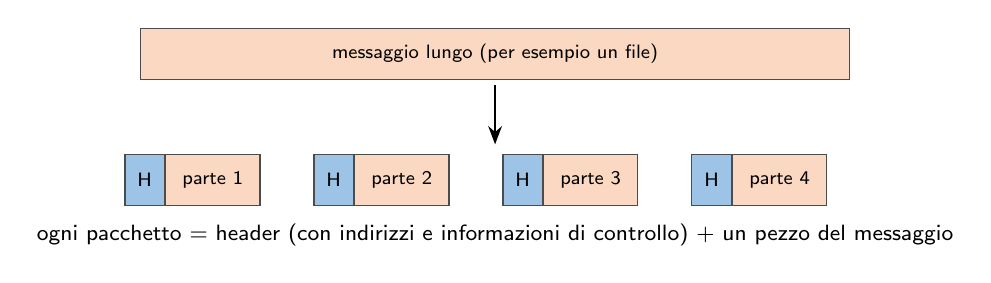
\begin{tikzpicture}[every node/.style={font=\scriptsize\sffamily}]
  \node[field, minimum width=9cm, fill=lapp!50] (m) at (0,0) {messaggio lungo (per esempio un file)};
  \foreach \i/\x in {1/-3.6, 2/-1.2, 3/1.2, 4/3.6} {
    \node[field, minimum width=0.5cm, fill=lnet] (h\i) at (\x-0.85,-1.6) {H};
    \node[field, minimum width=1.2cm, fill=lapp!50, right=0pt of h\i] {parte \i};
  }
  \draw[-{Stealth}, thick] (0,-0.4) -- (0,-1.15);
  \node[lbl] at (0,-2.3) {ogni pacchetto = header (con indirizzi e informazioni di controllo) + un pezzo del messaggio};
\end{tikzpicture}
\caption{Un messaggio viene diviso in pacchetti, ciascuno con il proprio header.}
\end{figure}

Perché dividere? Gestire un flusso continuo di bit sarebbe complicatissimo: se si verifica un
errore bisognerebbe ritrasmettere tutto. Con i pacchetti si ritrasmette \textbf{solo il pacchetto
danneggiato}, e più comunicazioni possono condividere lo stesso collegamento alternando i propri
pacchetti.

\dfn{Tempo di trasmissione e store-and-forward}{
    \begin{itemize}
      \item Un pacchetto di $L$ bit su un collegamento di rate $R$ bit/s richiede
            $\dfrac{L}{R}$ secondi per essere trasmesso.
      \item Un commutatore di pacchetto è \textbf{store-and-forward} (memorizza e inoltra): deve
            \textbf{ricevere l'intero pacchetto} prima di poterne trasmettere il primo bit sul
            collegamento successivo.
      \item Attraverso $N$ collegamenti di rate $R$, senza altro traffico, un pacchetto impiega
            $N\cdot\dfrac{L}{R}$ secondi.
    \end{itemize}
}

\begin{figure}[H]
\centering
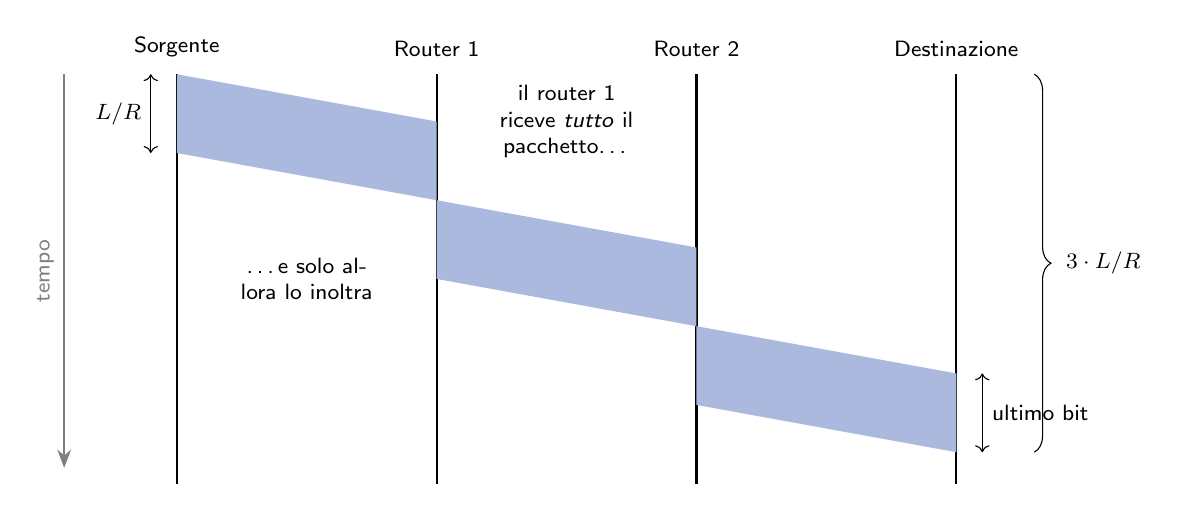
\begin{tikzpicture}[xscale=1.1, every node/.style={font=\footnotesize\sffamily}]
  \foreach \x/\n in {0/Sorgente, 3/Router 1, 6/Router 2, 9/Destinazione} {
    \node[above] at (\x,0.1) {\n};
    \draw[thick] (\x,0) -- (\x,-5.2);
  }
  \fill[netblue!40] (0,0) -- (3,-0.6) -- (3,-1.6) -- (0,-1.0) -- cycle;
  \fill[netblue!40] (3,-1.6) -- (6,-2.2) -- (6,-3.2) -- (3,-2.6) -- cycle;
  \fill[netblue!40] (6,-3.2) -- (9,-3.8) -- (9,-4.8) -- (6,-4.2) -- cycle;
  \draw[<->] (-0.3,0) -- node[left] {$L/R$} (-0.3,-1.0);
  \draw[<->] (9.3,-3.8) -- node[right] {ultimo bit} (9.3,-4.8);
  \node[lbl, text width=2.6cm, fill=white, inner sep=1pt] at (4.5,-0.6) {il router 1 riceve \emph{tutto} il pacchetto\dots};
  \node[lbl, text width=2.6cm, fill=white, inner sep=1pt] at (1.5,-2.6) {\dots e solo allora lo inoltra};
  \draw[decorate, decoration={brace, amplitude=6pt}] (9.9,0) -- (9.9,-4.8) node[midway, right=8pt] {$3\cdot L/R$};
  \draw[-{Stealth}, thick, black!50] (-1.3,0) -- node[left, rotate=90, anchor=south] {tempo} (-1.3,-5);
\end{tikzpicture}
\caption{Store-and-forward su tre collegamenti: ogni nodo aspetta l'intero pacchetto prima di inoltrarlo.}
\end{figure}

\begin{esempio}{Quanto ci mette un pacchetto}
Un pacchetto di $L = 10\,000$ bit attraversa $N = 3$ collegamenti da $R = 1$ Mb/s. Ogni
trasmissione dura $L/R = 10^4/10^6 = 0{,}01$ s, quindi il ritardo complessivo di trasmissione è
$3 \cdot 0{,}01 = 0{,}03$ s (trascurando la propagazione e le code).
\end{esempio}

\subsection{Code e perdite}

Ogni collegamento in uscita da un commutatore ha una \textbf{coda} (\emph{buffer}): tutto ciò che
deve essere trasmesso si mette in fila.

\begin{figure}[H]
\centering
\begin{tikzpicture}[every node/.style={font=\footnotesize\sffamily}]
  \node (A) at (-4,1) {\icon[0.9cm]{pc}};
  \node (B) at (-4,-1) {\icon[0.9cm]{laptop}};
  \node (R) at (0,0) {\icon[1.3cm]{router}};
  \draw[wired] (A) -- node[above, sloped, lbl] {100 Mb/s} (R);
  \draw[wired] (B) -- node[below, sloped, lbl] {100 Mb/s} (R);
  % coda
  \draw[thick] (1.1,0.35) -- (4.1,0.35); \draw[thick] (1.1,-0.35) -- (4.1,-0.35); \draw[thick] (4.1,0.35) -- (4.1,-0.35);
  \foreach \x in {1.3,1.8,2.3,2.8,3.3,3.8} \fill[netblue!60] (\x,-0.25) rectangle (\x+0.4,0.25);
  \node[above] at (2.6,0.4) {coda di uscita (piena)};
  \draw[wired, netred] (4.1,0) -- node[above, lbl, text=netred] {1,5 Mb/s} (6.5,0);
  \node at (7.2,0) {\icon[0.9cm]{router}};
  \fill[netred!70] (0.6,0.9) rectangle (1.0,1.3);
  \draw[netred, very thick] (0.5,0.8) -- (1.1,1.4); \draw[netred, very thick] (0.5,1.4) -- (1.1,0.8);
  \node[right, text=netred] at (1.2,1.1) {pacchetto scartato: \textbf{perdita}};
\end{tikzpicture}
\caption{Se i pacchetti arrivano più velocemente di quanto il collegamento riesca a smaltirli, si accodano; a coda piena vengono scartati.}
\end{figure}

\dfn{Ritardo di accodamento e perdita}{
    Se i pacchetti arrivano più velocemente di quanto il collegamento in uscita riesca a trasmetterli,
    \textbf{aspettano in coda} (ritardo di accodamento). Se la coda è piena, il pacchetto in arrivo
    viene \textbf{scartato}: è la \textbf{perdita di pacchetti} (\emph{packet loss}).
}

Da qui nascono le perdite su cui costruiremo gran parte del corso: TCP, per esempio, esiste proprio
per recuperarle.

% ══════════════════════════════════════════════════════════════
\section{Commutazione di circuito e commutazione di pacchetto}
% ══════════════════════════════════════════════════════════════

Ci sono due modi fondamentali di far attraversare una rete ai dati.

\subsection{Commutazione di circuito}

\dfn{Commutazione di circuito (circuit switching)}{
    Prima di trasmettere, la rete \textbf{riserva} lungo tutto il cammino una certa capacità di
    trasmissione, e la \textbf{mantiene dedicata} per tutta la durata della sessione; alla fine il
    circuito viene rilasciato. È il modello della rete \textbf{telefonica} tradizionale.
}

\begin{figure}[H]
\centering
\begin{tikzpicture}[every node/.style={font=\footnotesize\sffamily}]
  \node (A) at (0,0) {\icon[0.9cm]{pc}};
  \node (s1) at (2.5,1) {\icon[0.9cm]{switch}};
  \node (s2) at (2.5,-1.2) {\icon[0.9cm]{switch}};
  \node (s3) at (5.5,1) {\icon[0.9cm]{switch}};
  \node (s4) at (5.5,-1.2) {\icon[0.9cm]{switch}};
  \node (B) at (8,0) {\icon[1cm]{laptop}};
  \foreach \a/\b in {A/s2, s1/s2, s2/s4, s3/s4, s4/B, s1/s4} \draw[wired, black!40] (\a) -- (\b);
  \draw[pathhl] (A) -- (s1) -- (s3) -- (B);
  \node[text=netred] at (4,1.5) {circuito riservato per A--B};
  \node[lbl, text width=5cm] at (4,-2.3) {su ogni collegamento del cammino una parte della capacità è dedicata ad A e B, anche quando non parlano};
\end{tikzpicture}
\caption{Commutazione di circuito: un cammino e la sua capacità vengono riservati per l'intera sessione.}
\end{figure}

Come si ``ritaglia'' un circuito da un collegamento condiviso da più utenti? In due modi:

\begin{figure}[H]
\centering
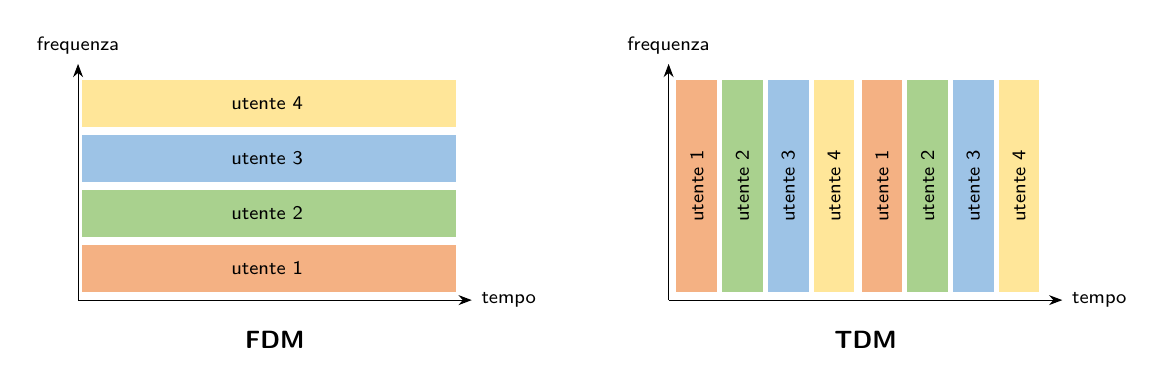
\begin{tikzpicture}[every node/.style={font=\scriptsize\sffamily}]
  \begin{scope}
    \draw[-{Stealth}] (0,0) -- (5,0) node[right] {tempo};
    \draw[-{Stealth}] (0,0) -- (0,3) node[above] {frequenza};
    \foreach \i/\c in {0/lapp, 1/ltra, 2/lnet, 3/llink} {
      \fill[\c] (0.05,0.1+\i*0.7) rectangle (4.8,0.7+\i*0.7);
      \node at (2.4,0.4+\i*0.7) {utente \the\numexpr\i+1\relax};
    }
    \node[font=\small\bfseries\sffamily] at (2.5,-0.5) {FDM};
  \end{scope}
  \begin{scope}[xshift=7.5cm]
    \draw[-{Stealth}] (0,0) -- (5,0) node[right] {tempo};
    \draw[-{Stealth}] (0,0) -- (0,3) node[above] {frequenza};
    \foreach \k in {0,1} \foreach \i/\c in {0/lapp, 1/ltra, 2/lnet, 3/llink} {
      \fill[\c] (0.1+\k*2.35+\i*0.58,0.1) rectangle (0.62+\k*2.35+\i*0.58,2.8);
      \node[rotate=90] at (0.36+\k*2.35+\i*0.58,1.45) {utente \the\numexpr\i+1\relax};
    }
    \node[font=\small\bfseries\sffamily] at (2.5,-0.5) {TDM};
  \end{scope}
\end{tikzpicture}
\caption{FDM: ogni utente ha una propria banda di frequenze, sempre. TDM: ogni utente ha tutta la banda, ma solo nel proprio intervallo di tempo (\emph{slot}), che si ripete ciclicamente.}
\end{figure}

\begin{itemize}
    \item \textbf{FDM} (\emph{Frequency Division Multiplexing}): lo spettro di frequenze del collegamento
          viene diviso in bande, e ogni circuito ne riceve una (come le stazioni radio).
    \item \textbf{TDM} (\emph{Time Division Multiplexing}): il tempo viene diviso in trame, ogni trama in
          intervalli (\emph{slot}), e ogni circuito riceve uno slot per trama.
\end{itemize}

\subsection{Commutazione di pacchetto}

\dfn{Commutazione di pacchetto (packet switching)}{
    La rete \textbf{non riserva nulla} in anticipo. Ogni pacchetto viene inviato indipendentemente e
    usa i collegamenti \textbf{su richiesta}; se un collegamento è occupato, il pacchetto \textbf{attende
    in coda}. È il modello di Internet.
}

\begin{figure}[H]
\centering
\begin{tikzpicture}[every node/.style={font=\footnotesize\sffamily}]
  \node (A) at (0,0.8) {\icon[0.8cm]{pc}};
  \node (C) at (0,-0.8) {\icon[0.9cm]{laptop}};
  \node (R) at (3,0) {\icon[1.2cm]{router}};
  \node (R2) at (8,0) {\icon[1.2cm]{router}};
  \draw[wired] (A) -- (R); \draw[wired] (C) -- (R); \draw[wired] (R) -- (R2);
  \foreach \x/\c in {4.2/netblue, 4.8/netgreen, 5.4/netgreen, 6.0/netblue, 6.6/netgreen} \fill[\c!70] (\x,0.18) rectangle (\x+0.45,0.55);
  \node[lbl, text width=6cm] at (5.5,-0.8) {i pacchetti di A (blu) e di C (verde) si alternano sullo stesso collegamento, secondo il bisogno del momento};
\end{tikzpicture}
\caption{Commutazione di pacchetto: la capacità del collegamento è condivisa dinamicamente (multiplexing statistico).}
\end{figure}

\subsection{Perché Internet ha scelto i pacchetti}

Il traffico dei calcolatori è \textbf{a raffica} (\emph{bursty}): brevi periodi di intensa attività
(si carica una pagina) alternati a lunghi silenzi (la si legge). Riservare un circuito
significherebbe tenere capacità inutilizzata per la maggior parte del tempo.

\begin{esempio}{10 utenti contro 35 utenti}
Un collegamento da 1 Mb/s è condiviso da utenti che, quando sono attivi, trasmettono a 100 kb/s,
ma sono attivi solo il 10\% del tempo.
\begin{itemize}
    \item Con la \textbf{commutazione di circuito} a ogni utente vanno riservati 100 kb/s sempre:
          il collegamento serve al massimo $1\,000/100 = \mathbf{10}$ utenti.
    \item Con la \textbf{commutazione di pacchetto} si possono servire \textbf{35} utenti: la probabilità
          che più di 10 di loro siano attivi \emph{nello stesso istante} è circa $0{,}0004$. Quasi sempre,
          quindi, il collegamento basta per tutti, con le stesse prestazioni percepite.
\end{itemize}
\end{esempio}

\begin{table}[H]
\centering
\begin{tabular}{p{3.3cm}p{5.5cm}p{5.5cm}}
\toprule
 & \textbf{Circuito} & \textbf{Pacchetto} \\
\midrule
Riserva di risorse & sì, per tutta la sessione & no, uso su richiesta \\
Prestazioni & garantite, costanti & variabili: code, ritardi, perdite \\
Uso della capacità & spreco nei silenzi & efficiente (multiplexing statistico) \\
Fase preliminare & instaurazione del circuito & nessuna \\
Esempio & rete telefonica tradizionale & Internet \\
\bottomrule
\end{tabular}
\caption{Commutazione di circuito e di pacchetto a confronto.}
\end{table}

\info{Anche la voce viaggia a pacchetti}{
    Quando telefonate con un'app di messaggistica non viene riservato alcun cammino: la vostra voce
    viene codificata e spedita a pacchetti (tipicamente con UDP, che vedremo), sperando che arrivino
    in tempo per ricostruire l'audio dall'altra parte.
}

% ══════════════════════════════════════════════════════════════
\section{Collegamenti punto-punto e multipunto}
% ══════════════════════════════════════════════════════════════

\dfn{Punto-punto e multipunto}{
    \begin{itemize}
      \item In un collegamento \textbf{punto-punto} esiste un collegamento \textbf{dedicato} tra
            \textbf{esattamente due} dispositivi, cablato o senza fili.
      \item In un collegamento \textbf{multipunto} (o \emph{broadcast}) \textbf{più dispositivi
            condividono lo stesso collegamento}, cablato o senza fili: quando uno trasmette, tutti
            gli altri lo sentono.
    \end{itemize}
}

\begin{figure}[H]
\centering
\begin{tikzpicture}[every node/.style={font=\footnotesize\sffamily}]
  \begin{scope}
    \node[font=\small\bfseries\sffamily] at (2.5,1.3) {Punto-punto};
    \node (a) at (0,0.4) {\icon[0.8cm]{pc}}; \node (b) at (5,0.4) {\icon[0.8cm]{pc}};
    \draw[wired] (a) -- node[above, lbl] {cablato} (b);
    \node (c) at (0,-1.2) {\icon[0.8cm]{laptop}}; \node (d) at (5,-1.2) {\icon[0.8cm]{laptop}};
    \draw[wireless] (c) -- node[above, lbl] {senza fili} (d);
    \node[lbl, text width=5cm] at (2.5,-2.3) {tutta la capacità è per quei due};
  \end{scope}
  \begin{scope}[xshift=8cm]
    \node[font=\small\bfseries\sffamily] at (2.5,1.3) {Multipunto};
    \draw[backbone] (-0.3,0.2) -- (5.3,0.2);
    \foreach \x [count=\i] in {0,1.7,3.4,5.0} { \node (p\i) at (\x,0.95) {\icon[0.6cm]{pc}}; \draw[wired] (\x,0.2) -- (p\i); }
    \node (ap) at (2.5,-1.1) {\icon[0.8cm]{accesspoint}};
    \foreach \x/\y in {0.2/-1.5, 4.8/-1.5, 1.0/-2.3, 4.0/-2.3} { \node (l) at (\x,\y) {\icon[0.55cm]{laptop}}; \draw[wireless] (ap) -- (l); }
    \node[lbl, text width=5cm] at (2.5,-3.1) {se due trasmettono insieme\dots?};
  \end{scope}
\end{tikzpicture}
\caption{Nel punto-punto il collegamento è di due soli dispositivi; nel multipunto il mezzo (un cavo condiviso o l'etere) è di tutti.}
\end{figure}

\warning{Il problema del mezzo condiviso}{
    Se due dispositivi su un collegamento multipunto trasmettono nello stesso istante, i segnali si
    sovrappongono e diventano incomprensibili: è una \textbf{collisione}. A gestire l'accesso al
    mezzo condiviso è un sottostrato del livello di collegamento chiamato \textbf{MAC}
    (\emph{Medium Access Control}), che studieremo nella Parte V.
}

La distinzione non è solo fisica: pesa anche sul progetto dei protocolli dei livelli superiori.
Notate che la rete Wi-Fi di casa, dal punto di vista logico, è un mezzo condiviso: tutti i
dispositivi ``parlano nell'aria'' vicino allo stesso access point.

% ══════════════════════════════════════════════════════════════
\section{Topologie di rete}
% ══════════════════════════════════════════════════════════════

\dfn{Topologia di rete}{
    La \textbf{topologia} di una rete è la disposizione dei suoi nodi e dei suoi collegamenti:
    \textbf{chi è collegato fisicamente con chi}, indipendentemente da ciò che gira sopra.
}

\info{Perché si chiama ``topologia''}{
    Il nome viene dal greco \emph{tópos}, ``luogo''. In matematica la topologia studia le proprietà
    che non cambiano deformando un oggetto senza strapparlo: \textbf{le distanze non contano}, conta solo
    \textbf{chi è connesso con chi}. Allo stesso modo, la topologia di una rete ignora quanto sono lunghi
    i cavi e dove stanno fisicamente gli apparati.
}

\begin{figure}[H]
\centering
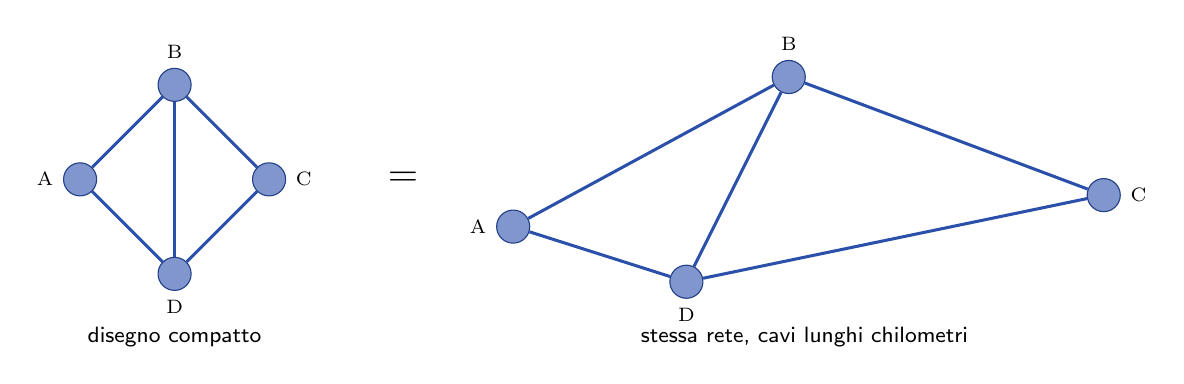
\begin{tikzpicture}
  \begin{scope}
    \node[gnode, label=left:{\scriptsize A}] (a) at (0,0) {};
    \node[gnode, label=above:{\scriptsize B}] (b) at (1.2,1.2) {};
    \node[gnode, label=right:{\scriptsize C}] (c) at (2.4,0) {};
    \node[gnode, label=below:{\scriptsize D}] (d) at (1.2,-1.2) {};
    \draw[wired] (a)--(b)--(c)--(d)--(a); \draw[wired] (b)--(d);
    \node[lbl] at (1.2,-2) {disegno compatto};
  \end{scope}
  \node[font=\Large] at (4.1,0) {$=$};
  \begin{scope}[xshift=5.5cm]
    \node[gnode, label=left:{\scriptsize A}] (a) at (0,-0.6) {};
    \node[gnode, label=above:{\scriptsize B}] (b) at (3.5,1.3) {};
    \node[gnode, label=right:{\scriptsize C}] (c) at (7.5,-0.2) {};
    \node[gnode, label=below:{\scriptsize D}] (d) at (2.2,-1.3) {};
    \draw[wired] (a)--(b)--(c)--(d)--(a); \draw[wired] (b)--(d);
    \node[lbl] at (3.7,-2) {stessa rete, cavi lunghi chilometri};
  \end{scope}
\end{tikzpicture}
\caption{Due disegni della stessa topologia: le lunghezze cambiano, i collegamenti no.}
\end{figure}

\begin{figure}[H]
    \centering
    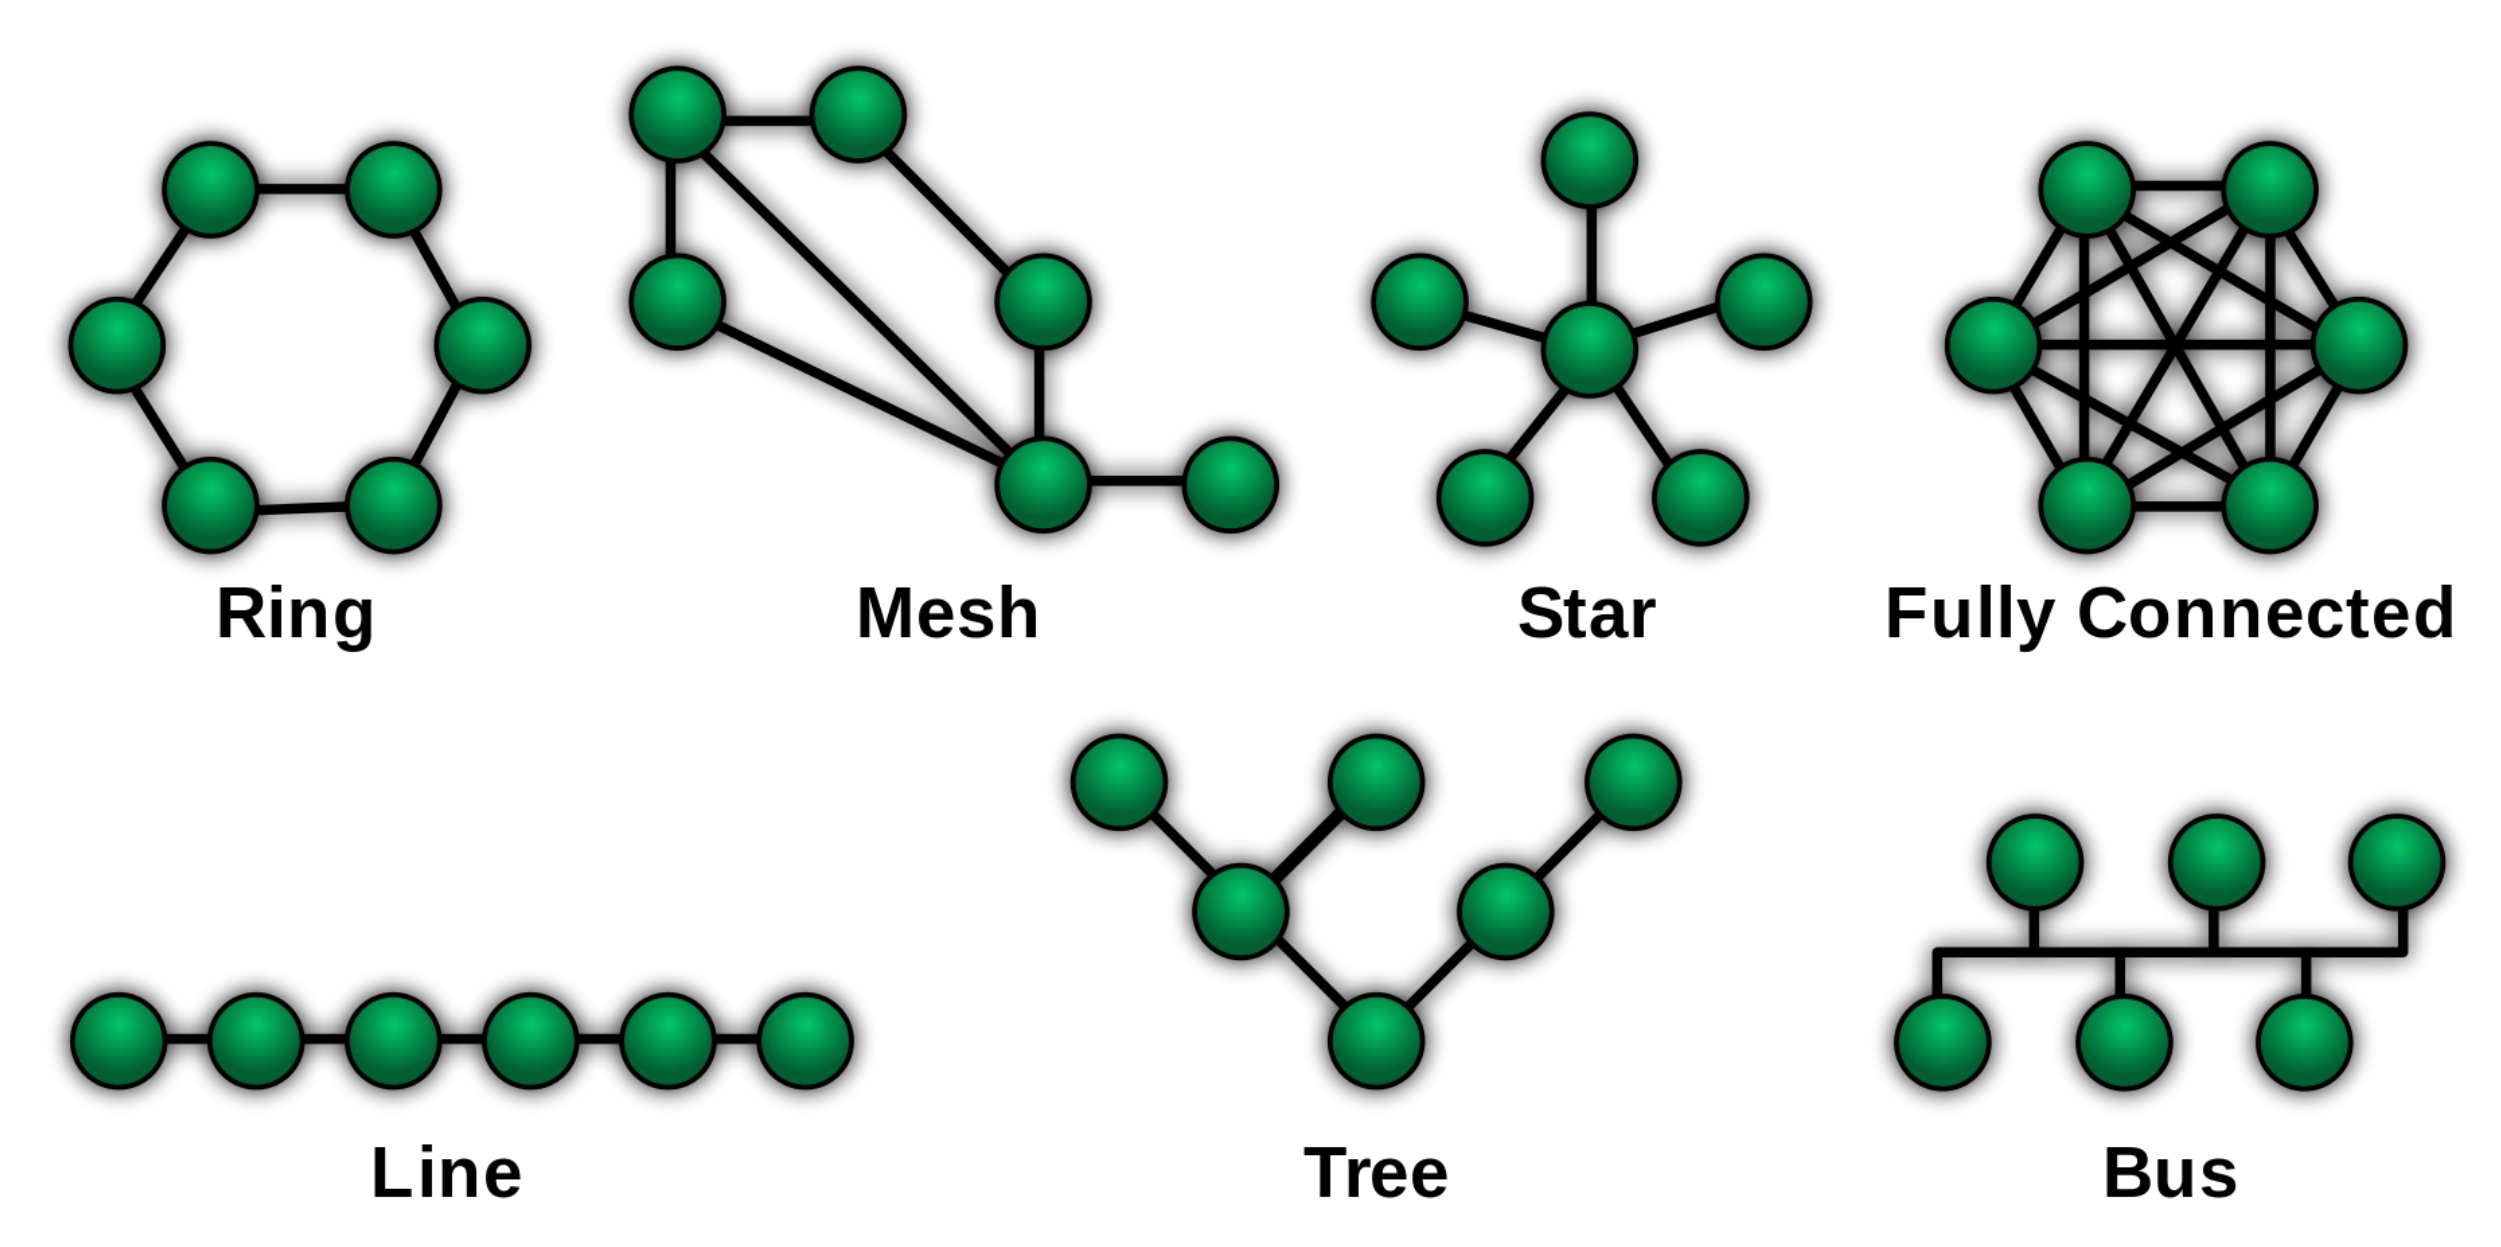
\includegraphics[width=0.65\linewidth]{cap01/topologie.png}
    \caption{Le topologie più comuni: anello, maglia, stella, completamente connessa, linea, albero, bus.}
\end{figure}

\subsection{Bus}

\begin{figure}[H]
\centering
\begin{minipage}{0.4\linewidth}\centering
  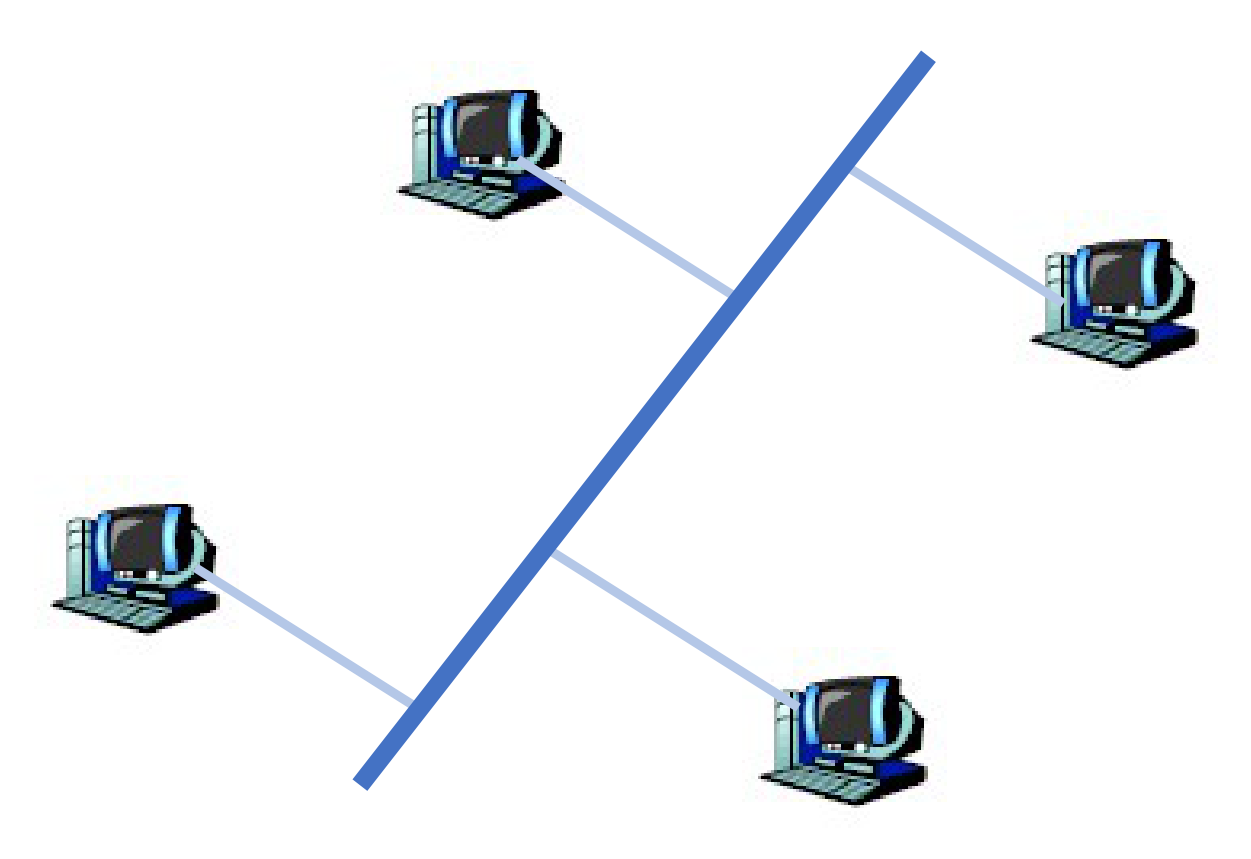
\includegraphics[width=0.85\linewidth]{cap01/topo_bus.png}
\end{minipage}\hfill
\begin{minipage}{0.56\linewidth}
Ogni host si collega a \textbf{un unico cavo condiviso} (il \emph{bus} o \emph{backbone}): ogni
trasmissione raggiunge tutti, e le \textbf{collisioni sono possibili}. È la topologia delle prime
reti Ethernet.
\begin{itemize}
  \item[\itick] semplice ed economica, adatta a reti piccole;
  \item[\itick] se si guasta il collegamento di un singolo host, gli altri non se ne accorgono;
  \item[\icross] se si \textbf{interrompe il bus}, la rete si spezza in due.
\end{itemize}
\textbf{Collegamenti}: 1 backbone e $n$ collegamenti di accesso ($1+n$).
\end{minipage}
\end{figure}

\subsection{Anello (ring)}

\begin{figure}[H]
\centering
\begin{minipage}{0.4\linewidth}\centering
  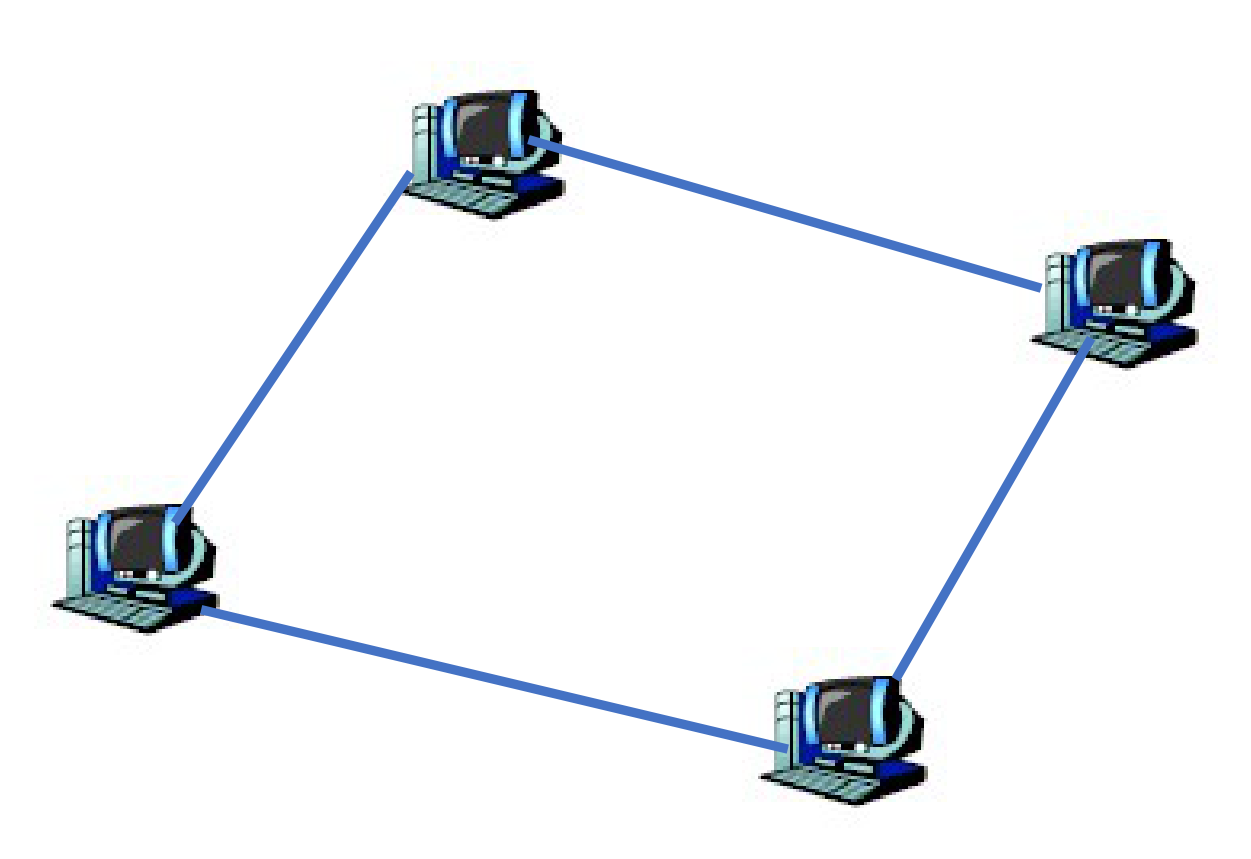
\includegraphics[width=0.85\linewidth]{cap01/topo_ring.png}
\end{minipage}\hfill
\begin{minipage}{0.56\linewidth}
Ogni host è collegato punto-punto con \textbf{esattamente altri due} (quello che lo precede e quello
che lo segue); il segnale viene inoltrato lungo l'anello, da un nodo all'altro, fino a destinazione.
Un esempio storico è il \emph{Token Ring} di IBM.
\begin{itemize}
  \item[\itick] economica, prestazioni migliori del bus;
  \item[\icross] aggiungere un nodo significa ``aprire'' l'anello;
  \item[\icross] come in una catena, l'anello più debole blocca tutto: un nodo malfunzionante può
        compromettere l'intera rete.
\end{itemize}
\textbf{Collegamenti}: $n$ collegamenti duplex.
\end{minipage}
\end{figure}

\subsection{Stella (star)}

\begin{figure}[H]
\centering
\begin{minipage}{0.4\linewidth}\centering
  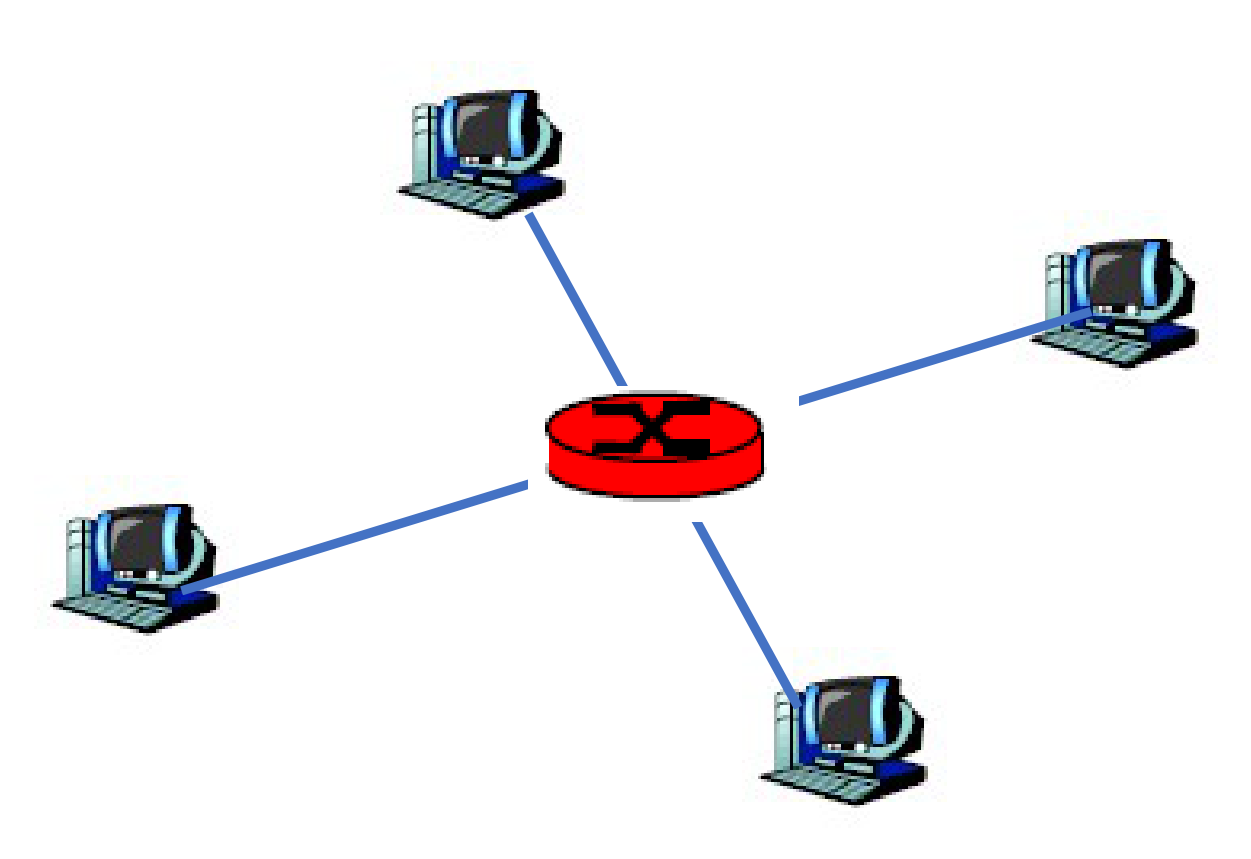
\includegraphics[width=0.85\linewidth]{cap01/topo_star.png}
\end{minipage}\hfill
\begin{minipage}{0.56\linewidth}
Gli host sono collegati \textbf{solo a un controllore centrale} (hub, switch o router), che smista
tutti i messaggi; non ci sono collegamenti diretti tra host. Il router di casa, con i dispositivi
collegati ad esso, forma proprio una stella.
\begin{itemize}
  \item[\itick] economica, semplice e \textbf{scalabile}: aggiungere un host = aggiungere un collegamento;
  \item[\itick] se un host si guasta, gli altri continuano a funzionare;
  \item[\icross] ogni host deve poter raggiungere il controllore;
  \item[\icross] il controllore è un \textbf{single point of failure}: se si guasta, non funziona più nulla.
\end{itemize}
\textbf{Collegamenti}: 1 controllore e $n$ collegamenti duplex.
\end{minipage}
\end{figure}

\subsection{Albero (tree)}

\begin{figure}[H]
\centering
\begin{minipage}{0.4\linewidth}\centering
  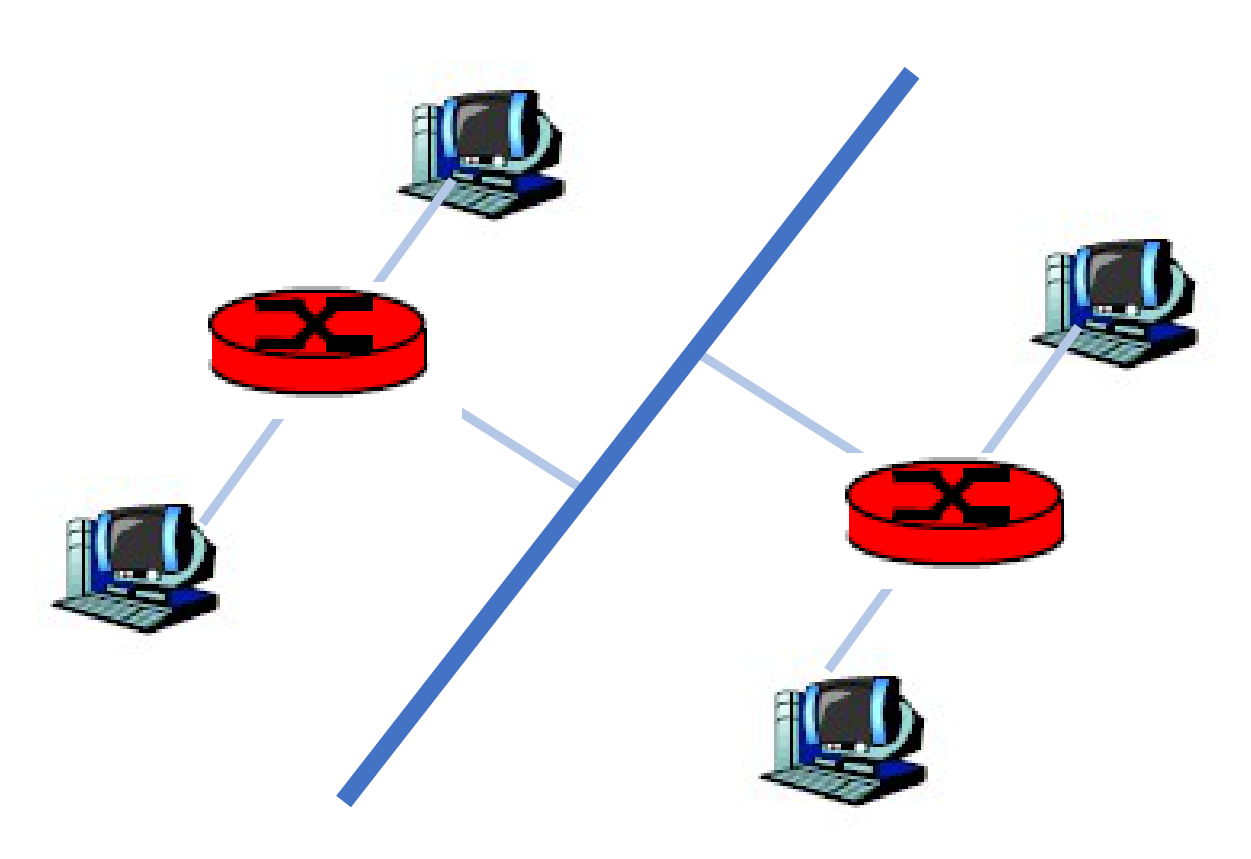
\includegraphics[width=0.85\linewidth]{cap01/topo_tree.png}
\end{minipage}\hfill
\begin{minipage}{0.56\linewidth}
\textbf{Più stelle collegate attraverso una dorsale} (un bus): è la forma che ha quasi ogni rete
reale di un edificio (una stella per piano, collegate da una dorsale).
\begin{itemize}
  \item[\itick] versatile, scalabile, ben supportata dai produttori di hardware e software;
  \item[\icross] più difficile da configurare di una singola stella: i controllori devono coordinarsi;
  \item[\icross] eredita la debolezza della dorsale: se si interrompe, si stacca un intero sottoalbero.
\end{itemize}
\end{minipage}
\end{figure}

\subsection{Linea (line)}

\begin{figure}[H]
\centering
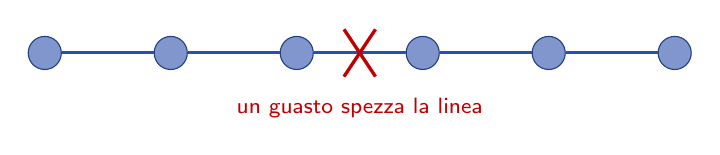
\begin{tikzpicture}
  \foreach \i in {0,...,5} \node[gnode] (n\i) at (\i*1.6,0) {};
  \foreach \i [evaluate=\i as \j using int(\i+1)] in {0,...,4} \draw[wired] (n\i) -- (n\j);
  \draw[netred, very thick] (3.8,-0.3) -- (4.2,0.3); \draw[netred, very thick] (3.8,0.3) -- (4.2,-0.3);
  \node[lbl, text=netred] at (4,-0.7) {un guasto spezza la linea};
\end{tikzpicture}
\caption{Topologia a linea (o a catena): $n$ nodi e $n-1$ collegamenti.}
\end{figure}

I nodi sono disposti in sequenza, ciascuno collegato al precedente e al successivo (ma, a
differenza dell'anello, il primo e l'ultimo non si chiudono). Servono solo $n-1$ collegamenti,
ma i messaggi tra nodi lontani attraversano tutti quelli in mezzo e un solo guasto divide la
rete.

\subsection{Maglia (mesh)}

\begin{figure}[H]
\centering
\begin{minipage}{0.4\linewidth}\centering
  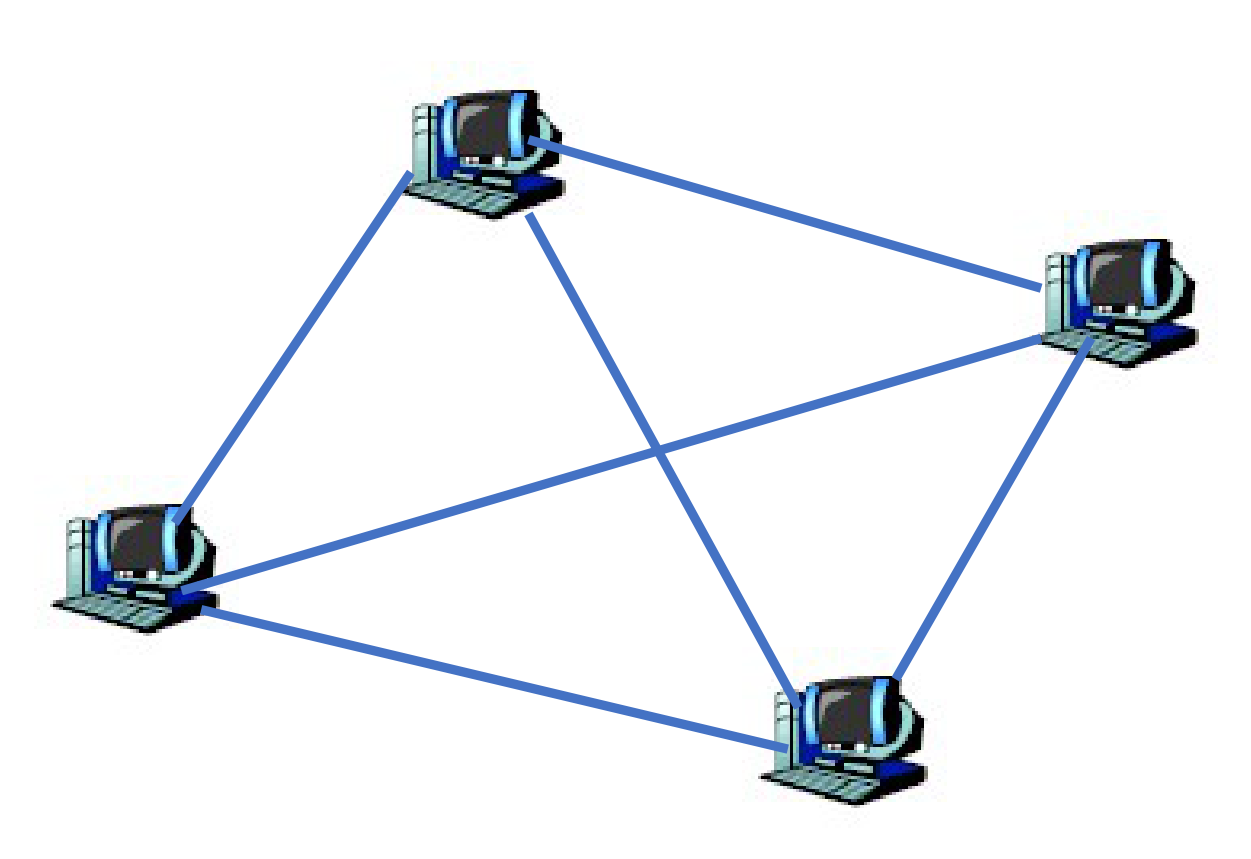
\includegraphics[width=0.85\linewidth]{cap01/topo_mesh.png}
\end{minipage}\hfill
\begin{minipage}{0.56\linewidth}
Gli host sono collegati punto-punto tra loro, \textbf{senza gerarchia}:
\begin{itemize}
  \item \textbf{full mesh} (completamente connessa): ogni nodo è collegato a tutti gli altri;
  \item \textbf{partial mesh}: ogni nodo è collegato solo ad alcuni.
\end{itemize}
\begin{itemize}
  \item[\itick] collegamenti \textbf{dedicati}: niente contesa come nel bus, buona robustezza;
  \item[\itick] se un collegamento cade, il traffico prende un'altra strada;
  \item[\icross] ogni nodo ha bisogno di tante porte quanti sono i suoi vicini;
  \item[\icross] \textbf{non scala}: una full mesh ha $\dfrac{n(n-1)}{2}$ collegamenti.
\end{itemize}
\end{minipage}
\end{figure}

\subsubsection*{Perché una full mesh ha $n(n-1)/2$ collegamenti}

In una full mesh ogni nodo è collegato a \textbf{tutti gli altri} $n-1$ nodi.

\begin{enumerate}
    \item Ogni nodo ha quindi $n-1$ collegamenti (e $n-1$ porte). Sommando su tutti gli $n$ nodi
          si ottengono $n(n-1)$ ``estremità di collegamento''.
    \item Ma ogni collegamento ha \textbf{due} estremità: il collegamento A--B è stato contato una
          volta partendo da A e una volta partendo da B.
    \item Dividendo per 2 si ottiene il numero di collegamenti: $\dfrac{n(n-1)}{2}$.
\end{enumerate}

In modo equivalente, il numero di collegamenti è il numero di \textbf{coppie non ordinate} di nodi,
cioè $\binom{n}{2}$; oppure si può contare aggiungendo i nodi uno alla volta: il secondo nodo
porta 1 collegamento nuovo, il terzo 2, il quarto 3, \dots, l'$n$-esimo $n-1$, e
$1+2+\dots+(n-1) = \dfrac{n(n-1)}{2}$.

\begin{figure}[H]
\centering
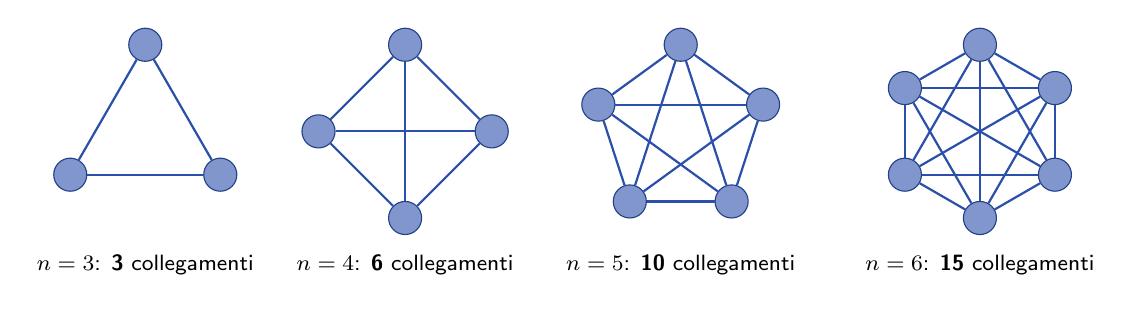
\begin{tikzpicture}
  \foreach \n/\x in {3/0, 4/3.3, 5/6.8, 6/10.6} {
    \begin{scope}[xshift=\x cm]
      \foreach \i in {1,...,\n} \node[gnode] (v\i) at ({90+360/\n*(\i-1)}:1.1) {};
      \foreach \i in {1,...,\n} \foreach \j in {1,...,\n} { \ifnum\i<\j \draw[wired, line width=0.8pt] (v\i) -- (v\j); \fi }
      \pgfmathtruncatemacro{\L}{\n*(\n-1)/2}
      \node[lbl] at (0,-1.7) {$n=\n$: \textbf{\L} collegamenti};
    \end{scope}
  }
\end{tikzpicture}
\caption{Full mesh con 3, 4, 5 e 6 nodi: i collegamenti crescono con il quadrato dei nodi.}
\end{figure}

\begin{esempio}{La crescita quadratica}
Con $n=10$ nodi servono $\dfrac{10\cdot 9}{2} = 45$ collegamenti; con $n=100$ ne servono
$\dfrac{100\cdot 99}{2} = 4\,950$, e ogni nodo avrebbe bisogno di 99 porte. Ecco perché la full mesh
è impraticabile oltre poche decine di nodi, e perché gli ISP non si collegano ``tutti con tutti''
(lo rivedremo parlando di IXP).
\end{esempio}

\subsection{Topologie ibride}

Le reti reali \textbf{mescolano} le topologie: ogni parte è scelta per il proprio segmento, e il
risultato non è nessuna delle forme componenti.

\begin{figure}[H]
\centering
\begin{minipage}{0.44\linewidth}\centering
  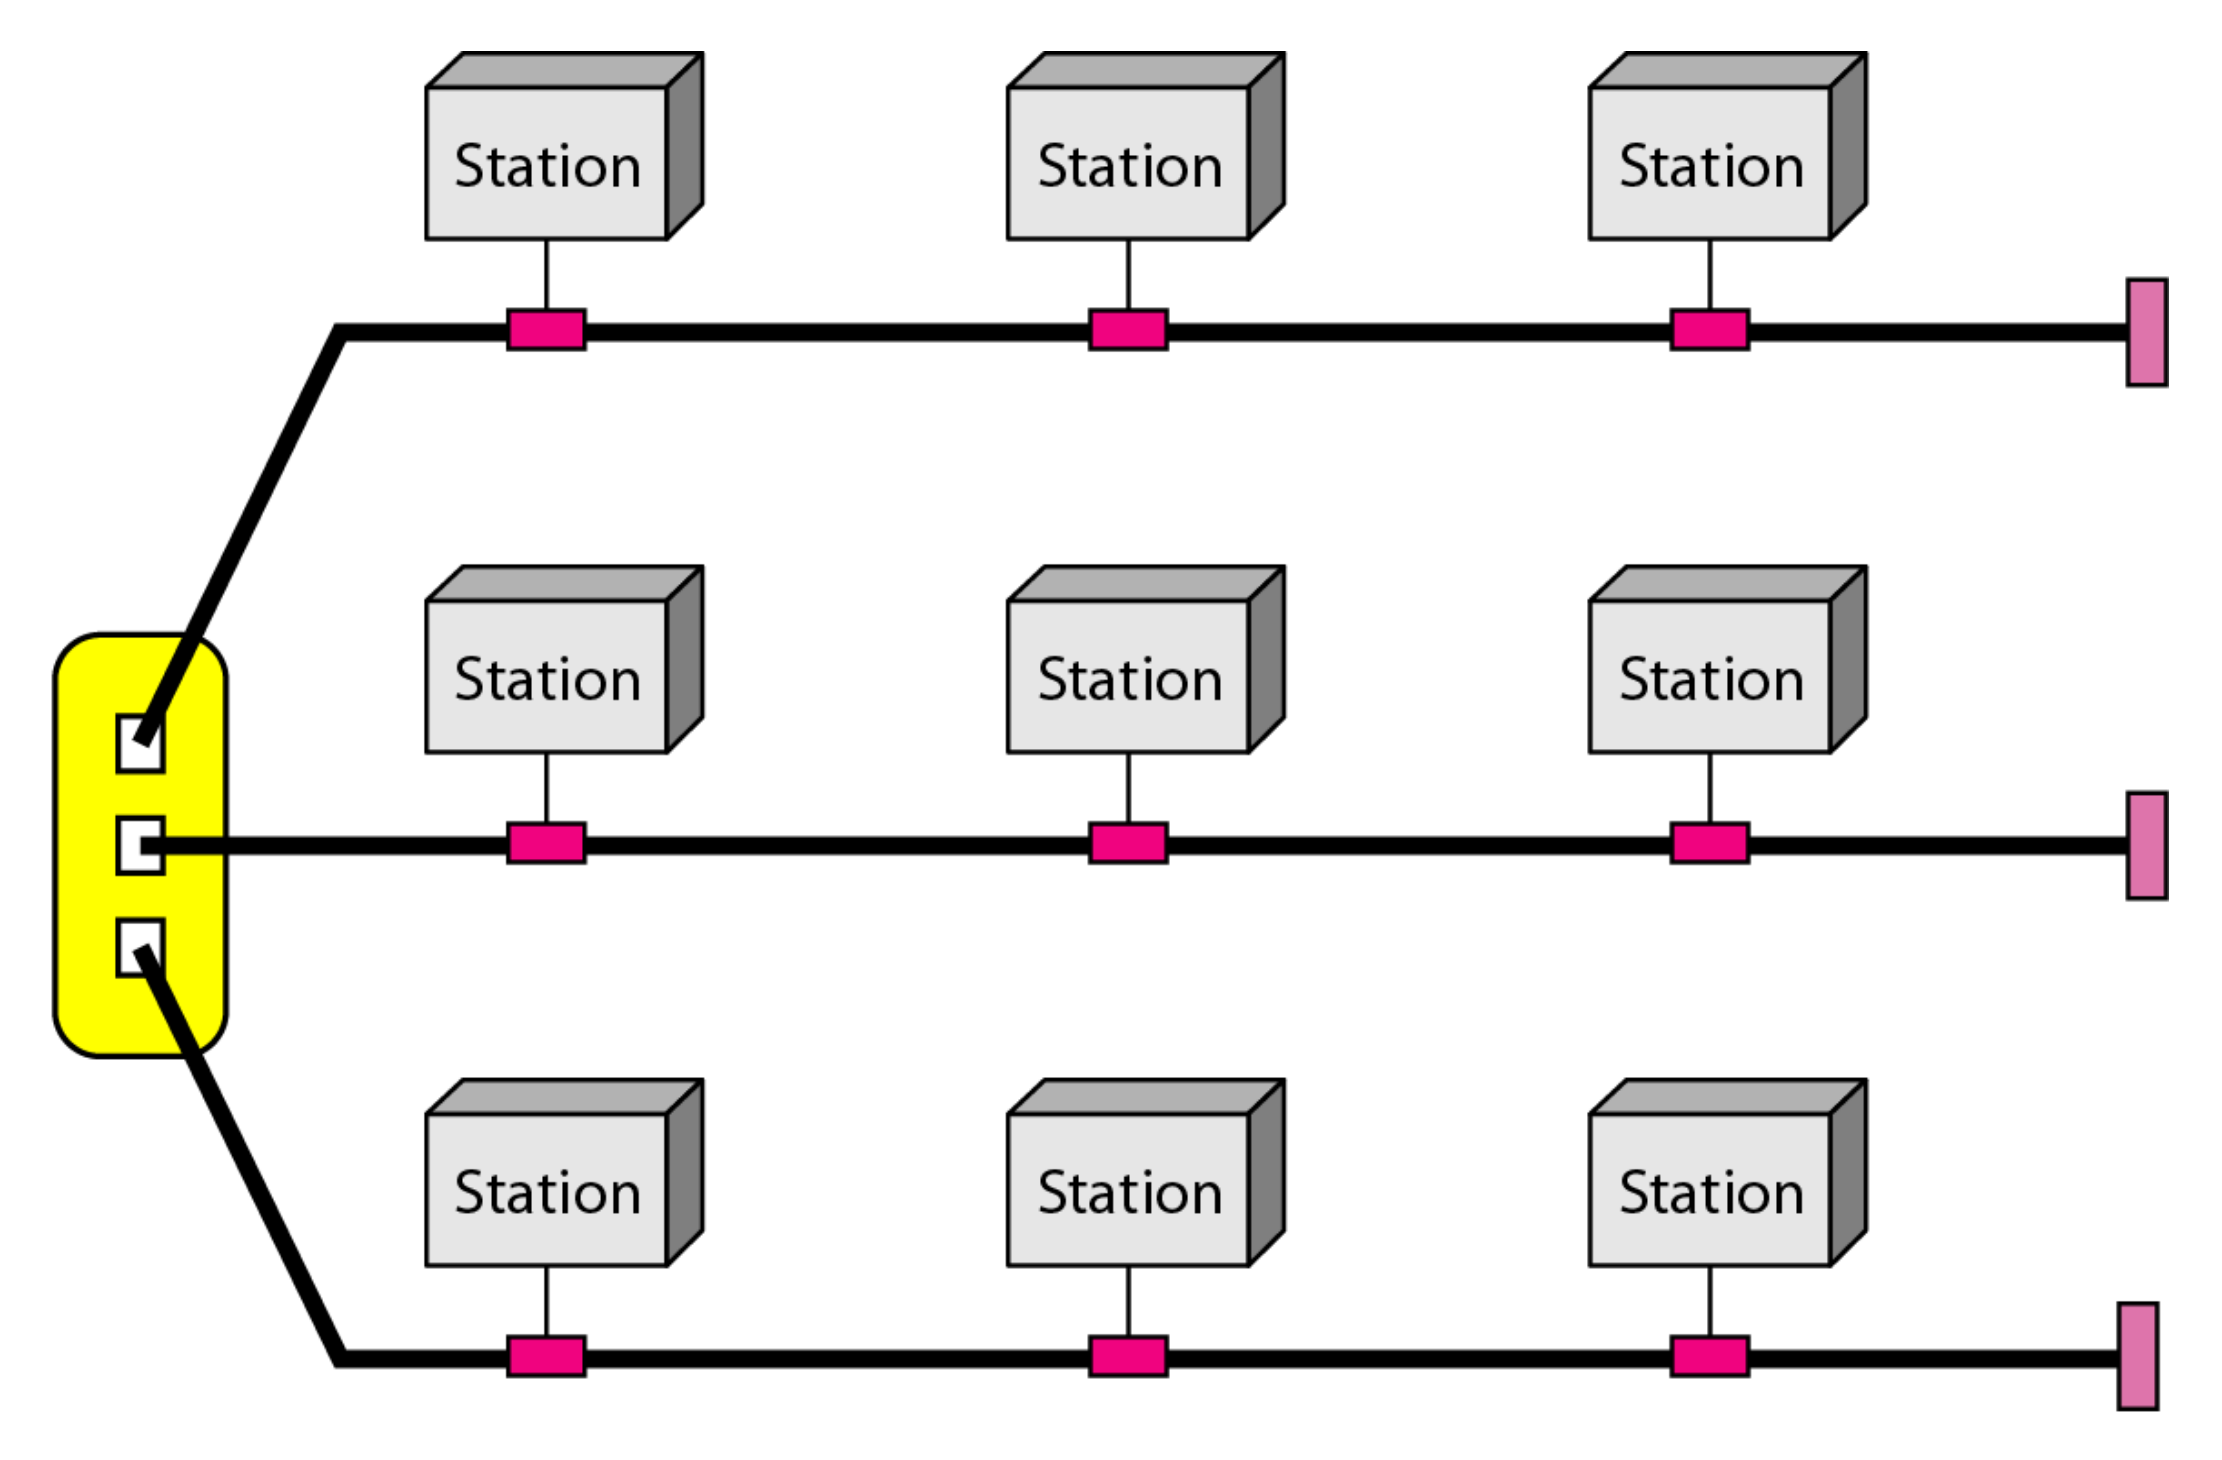
\includegraphics[width=\linewidth]{cap01/topo_ibrida.png}
\end{minipage}\hfill
\begin{minipage}{0.52\linewidth}\centering
\begin{tikzpicture}[every node/.style={font=\scriptsize\sffamily}]
  \node (hub) at (0,0) {\icon[1.1cm]{switch}};
  \node[below=-2pt of hub, lbl] {centro stella};
  \foreach \ang/\name in {90/Bus 1, 210/Bus 2, 330/Bus 3} {
    \begin{scope}[rotate=\ang]
      \draw[wired] (0.55,0) -- (1.3,0);
      \draw[backbone, line width=2pt] (1.3,-1.1) -- (1.3,1.1);
      \foreach \t in {-0.8,0,0.8} { \draw[wired, line width=0.7pt] (1.3,\t) -- (1.75,\t); \fill[netgreen] (1.75,\t) circle (3pt); }
    \end{scope}
  }
\end{tikzpicture}
\end{minipage}
\caption{Una dorsale a stella che collega tre reti a bus: una topologia ibrida.}
\end{figure}

Nell'esempio il centro della stella non è collegato a singoli host, ma a tre \emph{bus}, ciascuno
con i propri host. Le reti della TV via cavo, come vedremo, hanno una struttura ibrida di questo
tipo (albero di bus).

\subsection{Confronto tra le topologie}

\begin{table}[H]
\centering
\begin{tabular}{llp{4cm}p{4.2cm}}
\toprule
\textbf{Topologia} & \textbf{Collegamenti} & \textbf{Se si guasta un host} & \textbf{Se si guasta il mezzo} \\
\midrule
Bus & $1+n$ & nessun effetto sugli altri & la rete si divide \\
Anello & $n$ & l'anello può interrompersi & l'anello può interrompersi \\
Stella & $n$ & nessun effetto sugli altri & solo quell'host resta isolato \\
Albero & $n$ + dorsale & nessun effetto sugli altri & si isola un intero sottoalbero \\
Linea & $n-1$ & la linea si spezza & la linea si spezza \\
Mesh (full) & $n(n-1)/2$ & il traffico usa altri collegamenti & il traffico usa altri collegamenti \\
\bottomrule
\end{tabular}
\caption{Robustezza e costo delle topologie ($n$ = numero di host).}
\end{table}

\info{Robustezza contro costo}{
    La robustezza si compra con i collegamenti, e i collegamenti si comprano con porte e cavi: ogni
    rete reale è un compromesso tra le ultime due colonne della tabella e la seconda.
}

\warning{E la riservatezza?}{
    Una domanda frequente: una topologia come il bus, dove tutti ricevono tutto, è insicura? La
    riservatezza \textbf{non} dipende dalla topologia: è garantita da protocolli crittografici che
    funzionano a prescindere da chi può ascoltare le trasmissioni. Lo vedremo nella Parte VI.
}

% ══════════════════════════════════════════════════════════════
\section{Categorie di reti per estensione}
% ══════════════════════════════════════════════════════════════

Le reti si classificano in base alla \textbf{distanza} che coprono. Non è un dettaglio: la distanza
determina le \textbf{tecnologie} utilizzabili (quanto costa un cavo, quanto ritardo si accumula,
quanti errori ci sono).

\begin{figure}[H]
\centering
\begin{minipage}{0.3\linewidth}\centering
  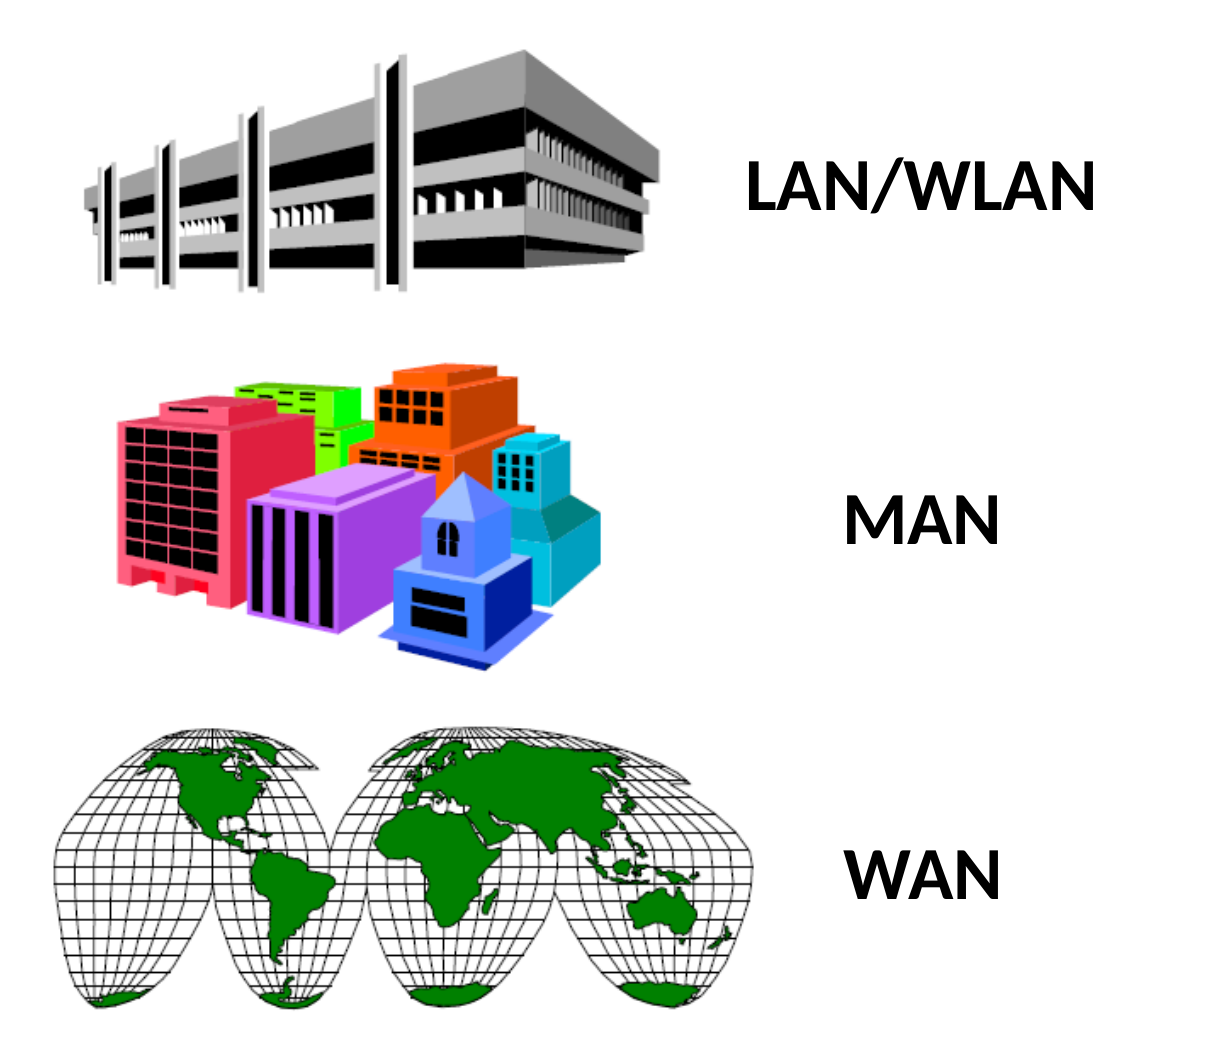
\includegraphics[width=0.9\linewidth]{cap01/categorie.png}
\end{minipage}\hfill
\begin{minipage}{0.66\linewidth}\centering
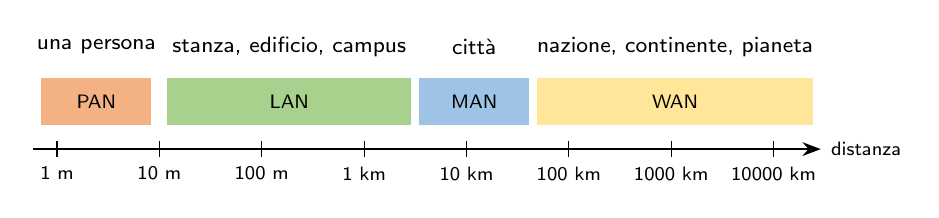
\begin{tikzpicture}[every node/.style={font=\scriptsize\sffamily}]
  \draw[-{Stealth}, thick] (0,0) -- (10,0) node[right] {distanza};
  \foreach \x/\t in {0.3/1 m, 1.6/10 m, 2.9/100 m, 4.2/1 km, 5.5/10 km, 6.8/100 km, 8.1/1000 km, 9.4/10000 km} {
    \draw (\x,0.1) -- (\x,-0.1); \node[below] at (\x,-0.1) {\t};
  }
  \fill[lapp] (0.1,0.3) rectangle (1.5,0.9); \node at (0.8,0.6) {PAN};
  \fill[ltra] (1.7,0.3) rectangle (4.8,0.9); \node at (3.25,0.6) {LAN};
  \fill[lnet] (4.9,0.3) rectangle (6.3,0.9); \node at (5.6,0.6) {MAN};
  \fill[llink] (6.4,0.3) rectangle (9.9,0.9); \node at (8.15,0.6) {WAN};
  \node[lbl] at (0.8,1.3) {una persona}; \node[lbl] at (3.25,1.3) {stanza, edificio, campus};
  \node[lbl] at (5.6,1.3) {città}; \node[lbl] at (8.15,1.3) {nazione, continente, pianeta};
\end{tikzpicture}
\end{minipage}
\caption{Le categorie di reti per estensione (i confini sono indicativi).}
\end{figure}

\begin{itemize}
    \item \textbf{PAN} (\emph{Personal Area Network}): attorno a una persona, pochi metri.
    \item \textbf{LAN} (\emph{Local Area Network}): un edificio o un campus.
    \item \textbf{MAN} (\emph{Metropolitan Area Network}): una città.
    \item \textbf{WAN} (\emph{Wide Area Network}): una nazione, un continente o più.
\end{itemize}

\warning{Zone grigie}{
    La classificazione si fa ``a spanne'': i confini non sono rigidi e una rete può stare a cavallo
    di due categorie. L'importante è capire l'ordine di grandezza e le conseguenze tecnologiche.
}

\subsection{PAN --- Personal Area Network}

\begin{figure}[H]
\centering
\begin{minipage}{0.36\linewidth}\centering
  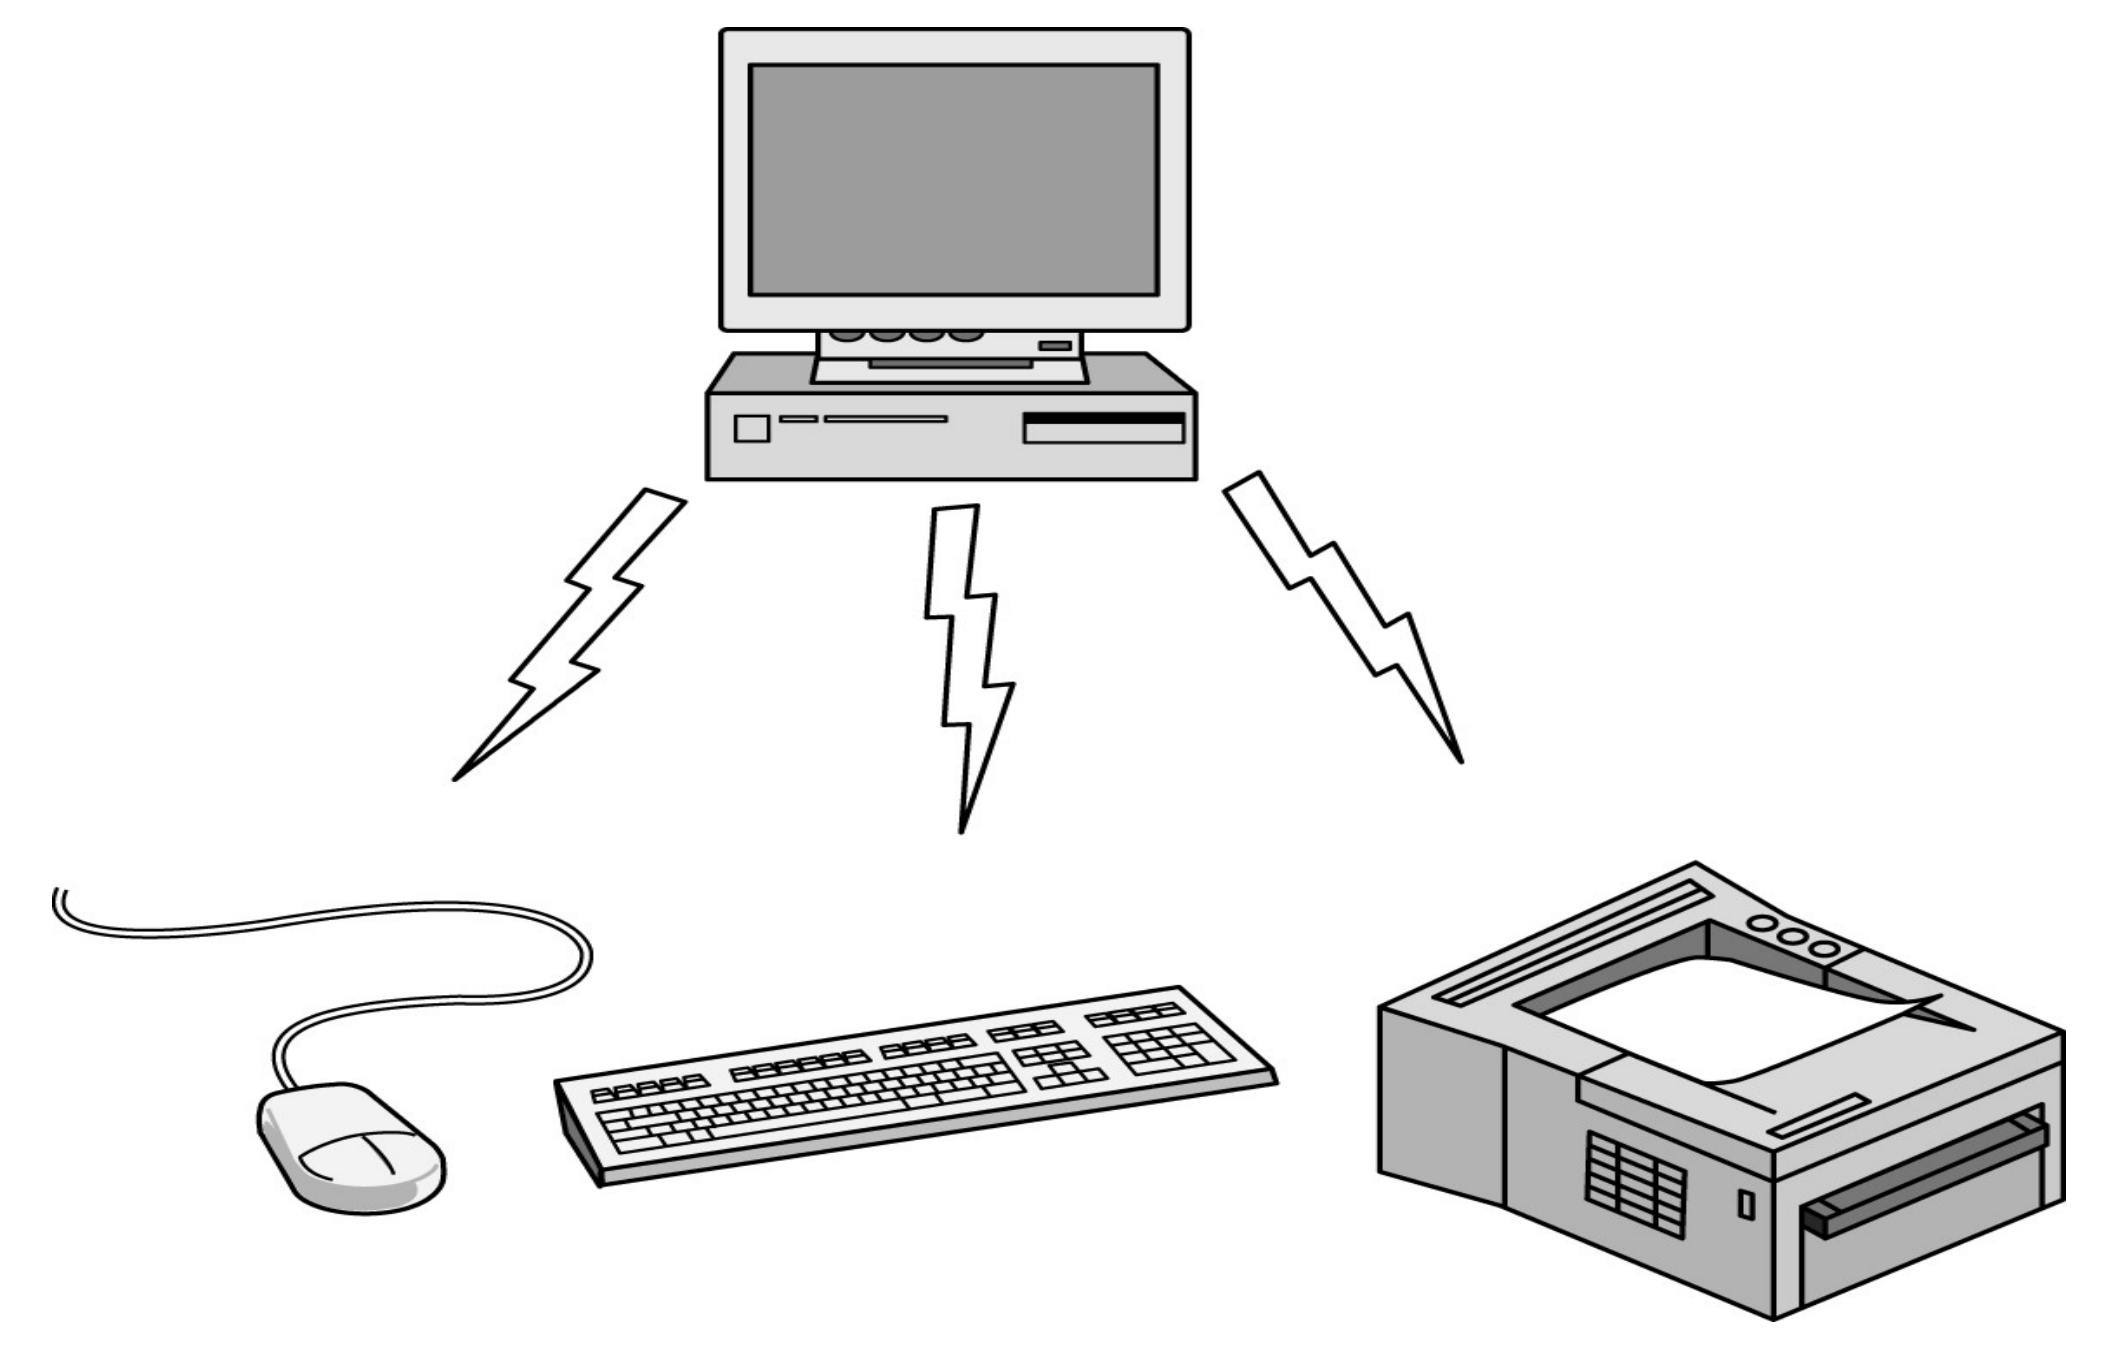
\includegraphics[width=0.9\linewidth]{cap01/pan.png}
\end{minipage}\hfill
\begin{minipage}{0.6\linewidth}
Una PAN collega i dispositivi nel raggio d'azione di una persona: cuffie, tastiera, mouse, orologio,
stampante. L'esempio tipico è \textbf{Bluetooth}, una rete senza fili a corto raggio che elimina i
cavi da cercare e collegare. Bluetooth funziona in modalità \textbf{master--slave}: il calcolatore
(master) dice alle periferiche (slave) quando e su quale frequenza possono trasmettere.
\end{minipage}
\caption{Una PAN Bluetooth.}
\end{figure}

\subsection{LAN --- Local Area Network}

\dfn{LAN}{
    Una \textbf{LAN} è una rete \textbf{privata} all'interno di un edificio o di un campus. Le sue
    dimensioni sono limitate, quindi il \textbf{tempo di trasmissione nel caso peggiore è noto} in
    anticipo; ha \textbf{bassa latenza}, \textbf{pochi errori} e oggi velocità da 100 Mb/s a decine di Gb/s.
}

\begin{figure}[H]
    \centering
    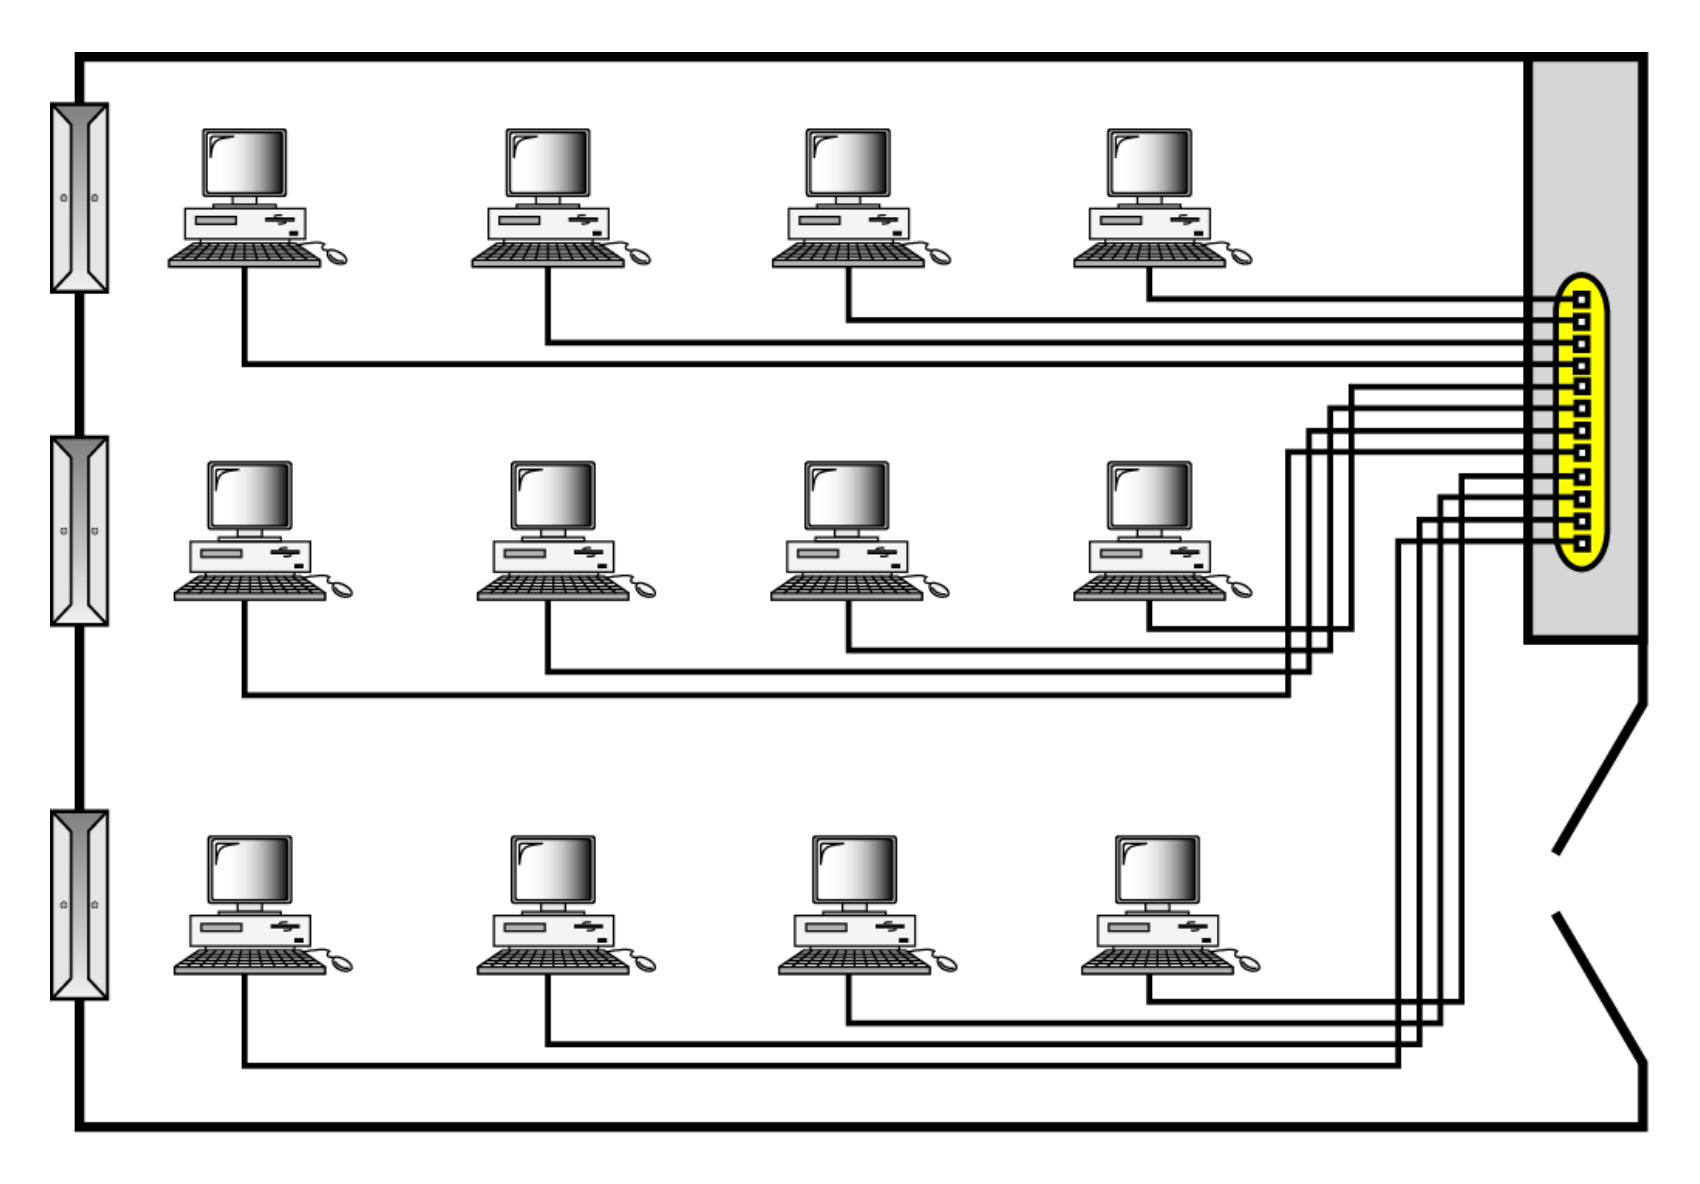
\includegraphics[width=0.45\linewidth]{cap01/lan_switch.png}
    \caption{Una LAN che collega dodici computer a uno switch.}
\end{figure}

Le LAN possono essere \textbf{senza fili} o \textbf{cablate}:

\begin{figure}[H]
    \centering
    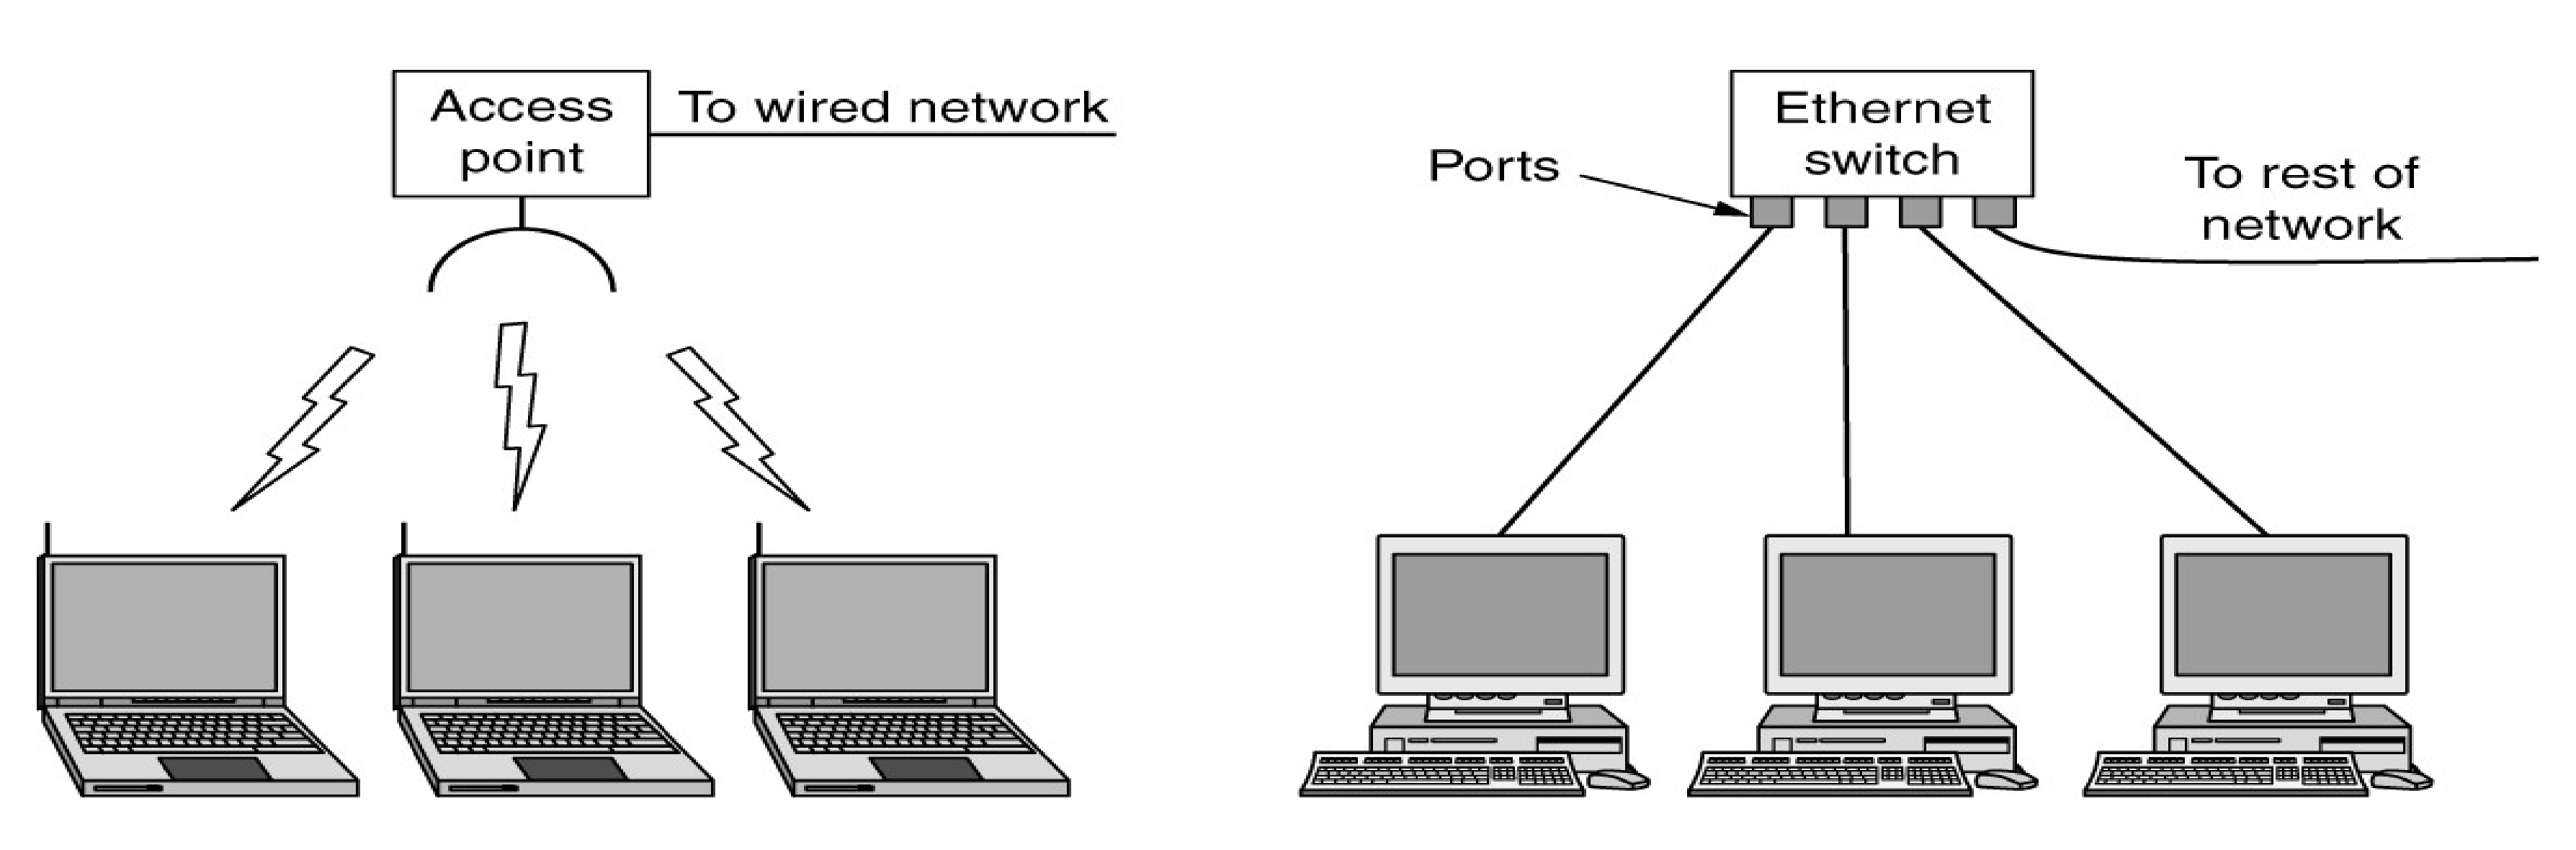
\includegraphics[width=0.8\linewidth]{cap01/lan_wireless_wired.png}
    \caption{A sinistra una rete wireless 802.11: ogni macchina parla con un access point, che inoltra i dati verso la rete cablata. A destra una rete Ethernet commutata: ogni macchina ha il proprio cavo verso uno switch, che inoltra i frame in base all'indirizzo.}
\end{figure}

\begin{itemize}
    \item \textbf{Wireless LAN} (WLAN): lo standard è \textbf{IEEE 802.11}, il Wi-Fi di casa.
    \item \textbf{LAN cablata}: tipicamente \textbf{Ethernet commutata} (\emph{switched Ethernet}), con il
          classico cavo di rete. Se il Wi-Fi in camera va male, un cavo Ethernet collegato al router
          garantisce una banda più stabile.
\end{itemize}

\subsubsection*{La rete di casa}

La rete domestica è una LAN, ma è \textbf{la LAN con i requisiti più difficili}:

\begin{itemize}
    \item viene installata da qualcuno che non leggerà il manuale: deve \textbf{funzionare da sola},
          appena tirato fuori il router dalla scatola (vedremo i protocolli, come DHCP, che lo rendono
          possibile);
    \item i dispositivi vengono comprati uno alla volta, nel corso degli anni, da produttori diversi, e
          devono comunque \textbf{funzionare insieme};
    \item i margini di guadagno sono bassi, mentre sicurezza, affidabilità e interoperabilità costano;
    \item un elettrodomestico insicuro non è un file perso: è una serratura che qualcun altro può aprire.
\end{itemize}

\info{IoT: prima un problema di sicurezza}{
    È nelle case che l'Internet of Things arriva davvero (televisore, frigorifero, telecamere,
    tapparelle), ed è per questo che l'IoT è un problema di \textbf{sicurezza} prima ancora che di rete.
}

\subsection{MAN --- Metropolitan Area Network}

\dfn{MAN}{
    Una \textbf{MAN} copre l'area di una \textbf{città}. Collega tra loro edifici, quartieri o
    abitazioni di un'area urbana, tipicamente con un'infrastruttura posseduta da un unico operatore.
}

L'esempio più noto è la \textbf{rete della televisione via cavo}, molto diffusa in Nord America.

\begin{figure}[H]
    \centering
    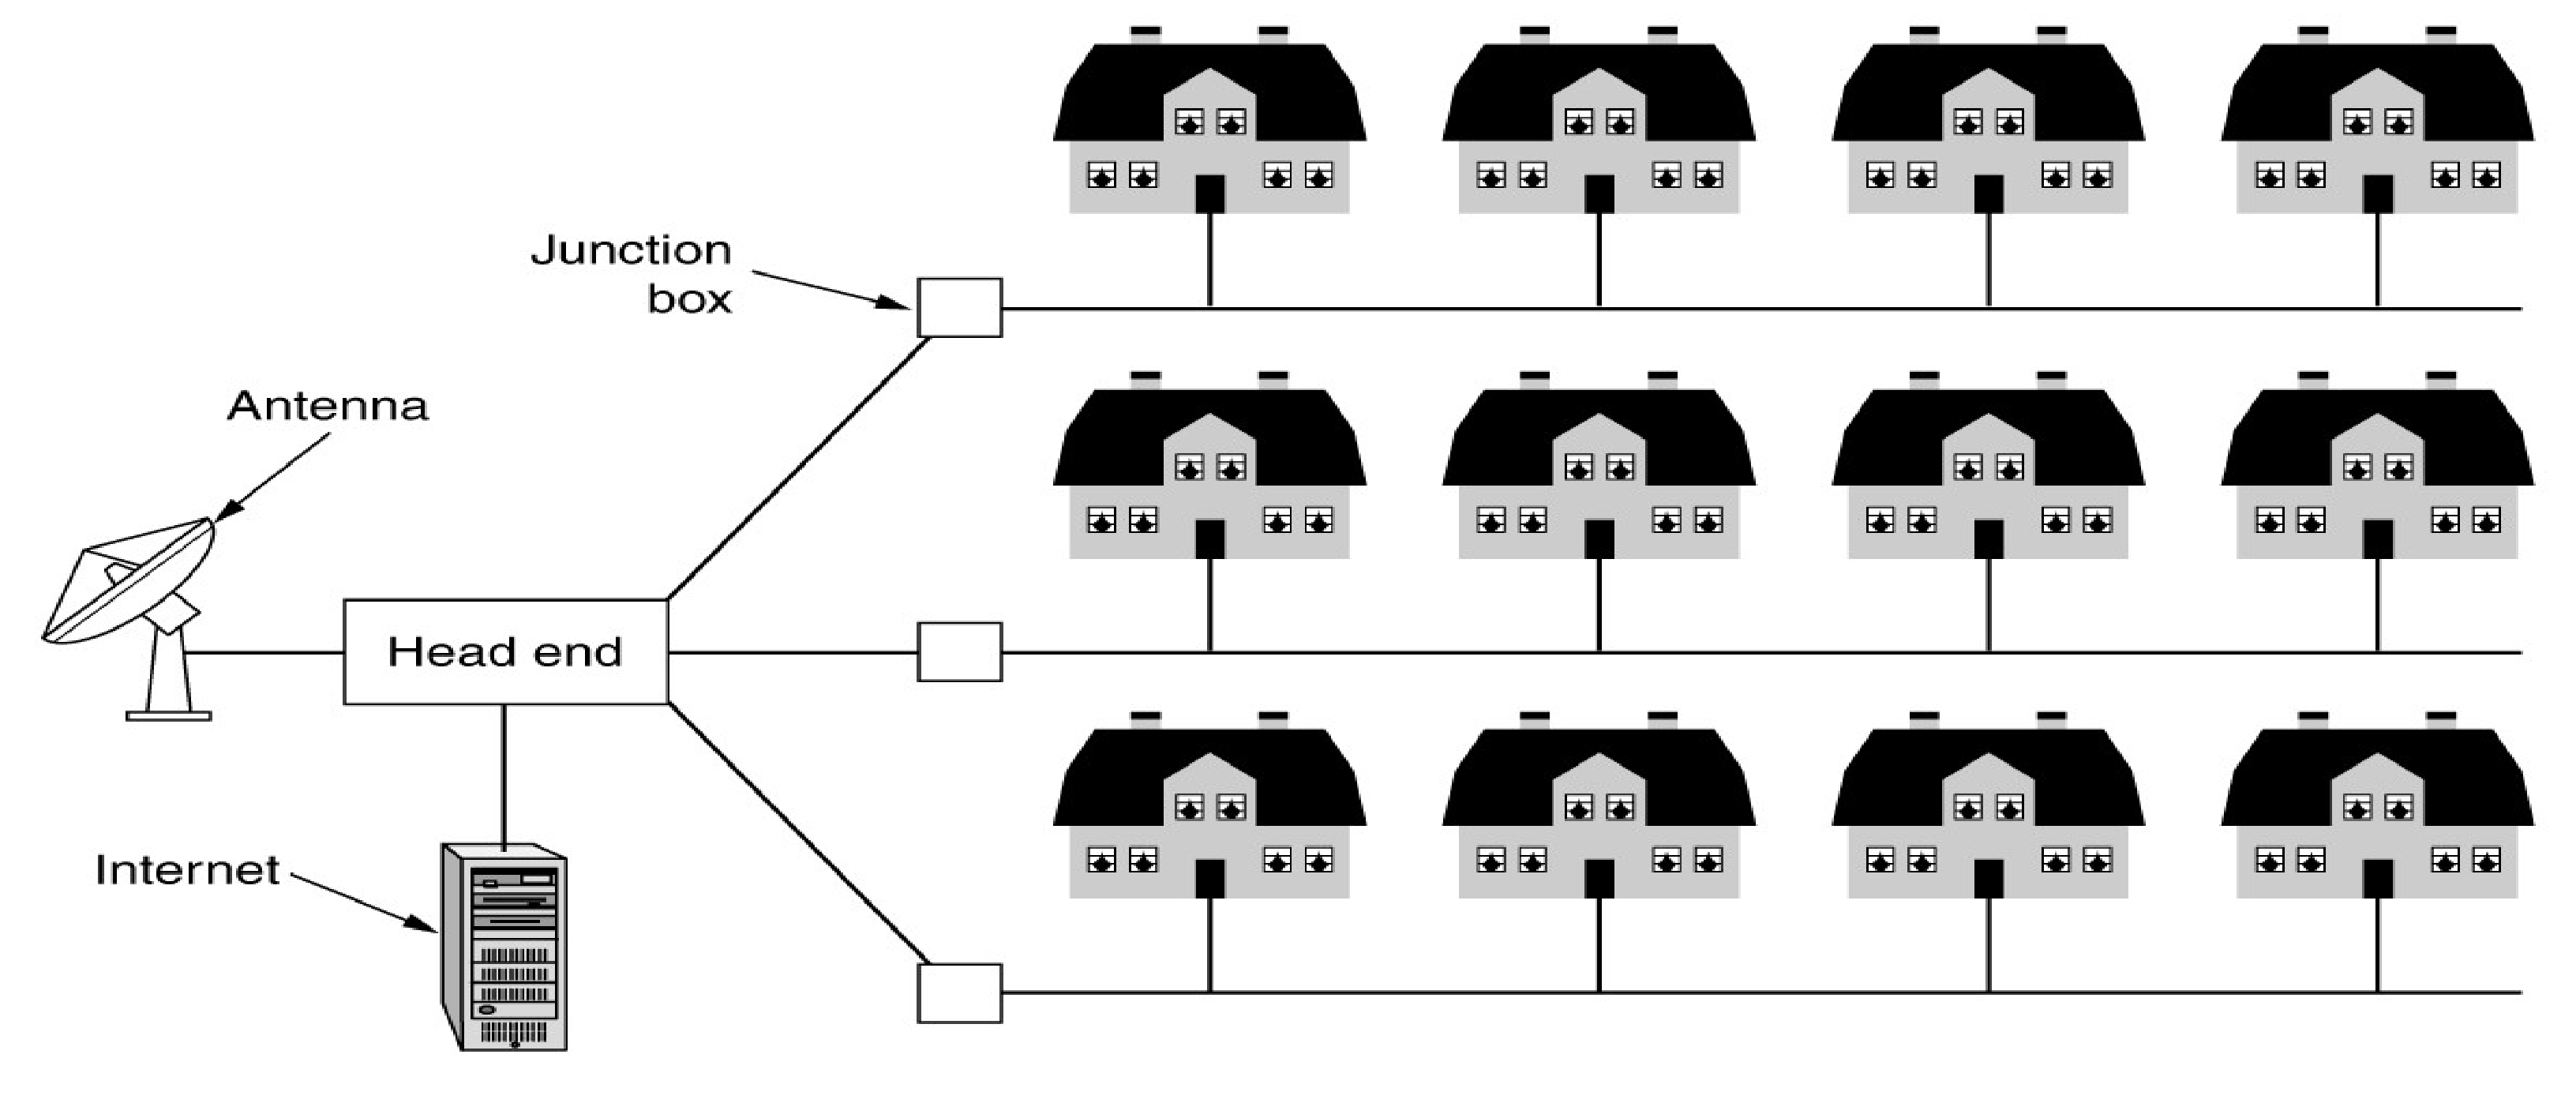
\includegraphics[width=0.62\linewidth]{cap01/man_cavo.png}
    \caption{Una MAN via cavo: televisione e Internet entrano nella stessa \emph{head-end} e vengono distribuite alle case.}
\end{figure}

\begin{itemize}
    \item Al centro c'è la \textbf{head-end} (\emph{cable head-end}, o \emph{cable modem termination
          system}): riceve i canali TV dall'\textbf{antenna} e, da quando la rete è usata anche per
          Internet, è collegata a \textbf{Internet}.
    \item Dalla head-end partono cavi che, attraverso delle \textbf{scatole di giunzione}
          (\emph{junction box}), raggiungono le strade; lungo ogni strada le case sono collegate allo
          stesso cavo, come su un \textbf{bus}. Nel complesso la rete è un \textbf{albero di bus}.
    \item La rete era nata per distribuire la televisione \textbf{in una sola direzione}. È stata poi
          trasformata in un servizio Internet \textbf{bidirezionale} usando le parti dello spettro di
          frequenze lasciate libere dai canali TV.
\end{itemize}

Altri esempi di MAN sono le reti in fibra ottica che collegano le sedi di un'università o gli
uffici pubblici di una città.

\subsection{WAN --- Wide Area Network}

Una WAN copre una nazione o un continente. L'esempio classico del Tanenbaum è un'azienda con
tre uffici in Australia: Perth, Melbourne e Brisbane.

\dfn{Host e subnet in una WAN}{
    In una WAN:
    \begin{itemize}
      \item le macchine che eseguono le applicazioni sono gli \textbf{host};
      \item tutto ciò che trasporta i loro messaggi, cioè \textbf{linee di trasmissione e router},
            forma la \textbf{subnet} (sottorete di comunicazione). La subnet di solito è posseduta da
            qualcun altro, tipicamente una compagnia di telecomunicazioni.
    \end{itemize}
}

\warning{Due significati di ``subnet''}{
    Qui \emph{subnet} (terminologia del Tanenbaum) indica l'infrastruttura di trasporto di una WAN.
    Nella Parte IV la stessa parola indicherà un \emph{blocco di indirizzi IP} (subnetting). Non
    confondete i due usi.
}

La complessità di una WAN sta soprattutto nel \textbf{modo} in cui si realizzano i collegamenti
tra sedi lontane. Ci sono tre soluzioni tipiche.

\subsubsection*{1. Linee dedicate (leased lines)}

\begin{figure}[H]
    \centering
    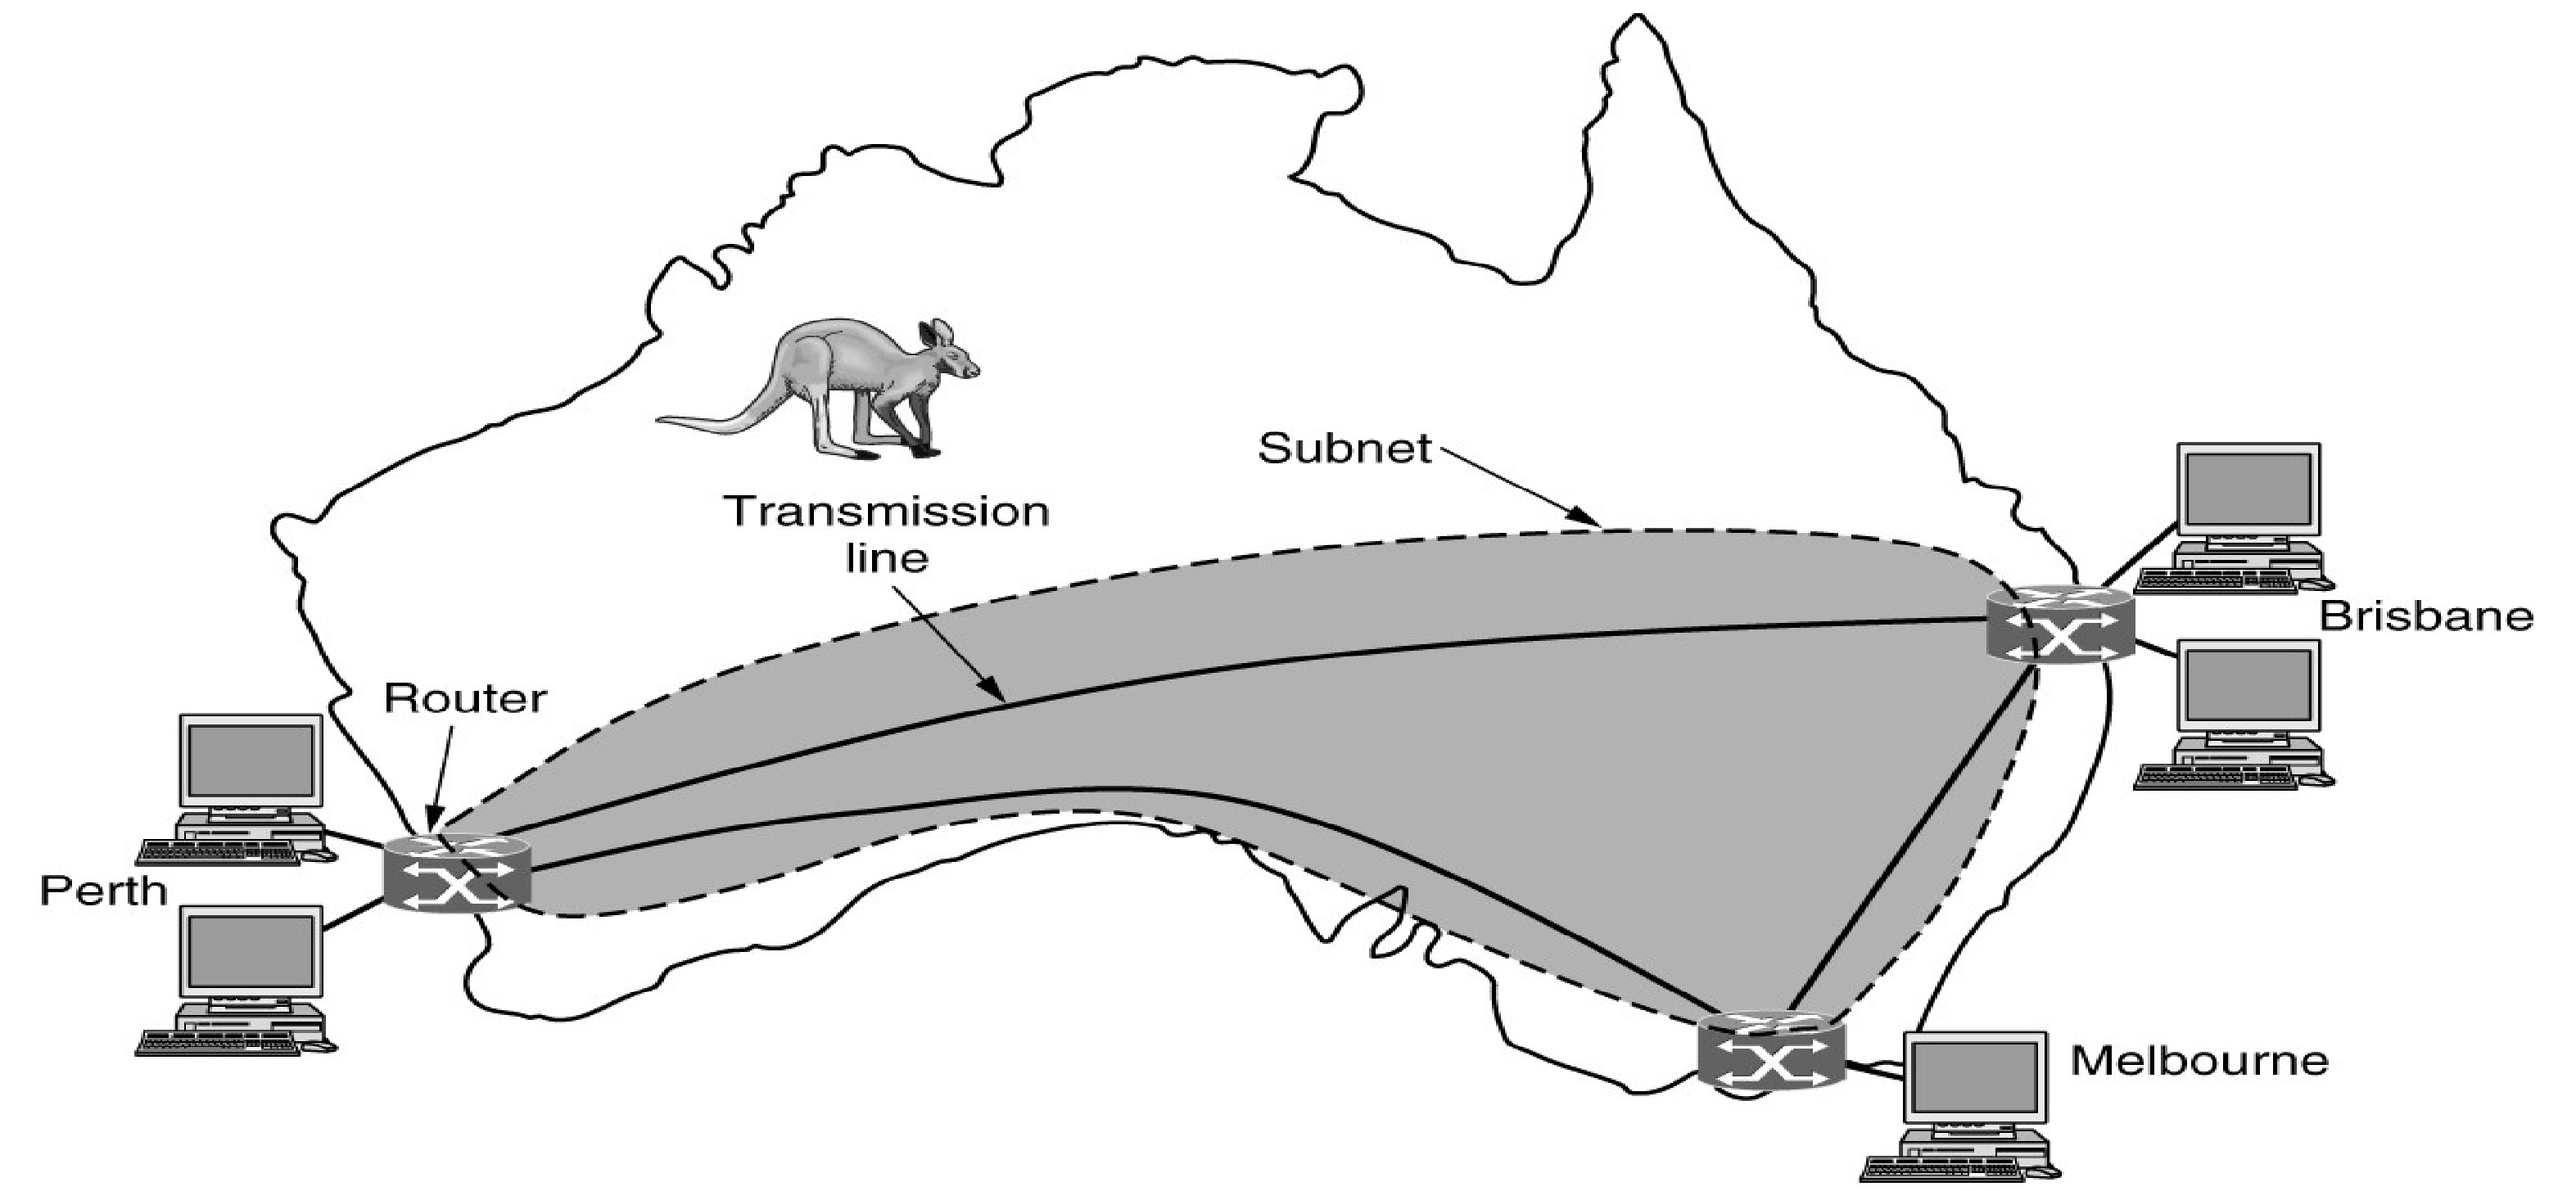
\includegraphics[width=0.55\linewidth]{cap01/wan_leased.png}
    \caption{Tre uffici collegati da linee affittate: la subnet (in grigio) è fatta di router e linee di trasmissione.}
\end{figure}

L'azienda \textbf{affitta linee di trasmissione} da un operatore e le collega con i propri router.
La capacità delle linee è sua, garantita e prevedibile; ma è la soluzione più \textbf{costosa} e meno
flessibile (aggiungere una sede significa affittare nuove linee). Stendere i propri cavi
attraverso l'Australia, del resto, non è alla portata di quasi nessuno.

\subsubsection*{2. Collegamenti virtuali su Internet (VPN)}

\begin{figure}[H]
    \centering
    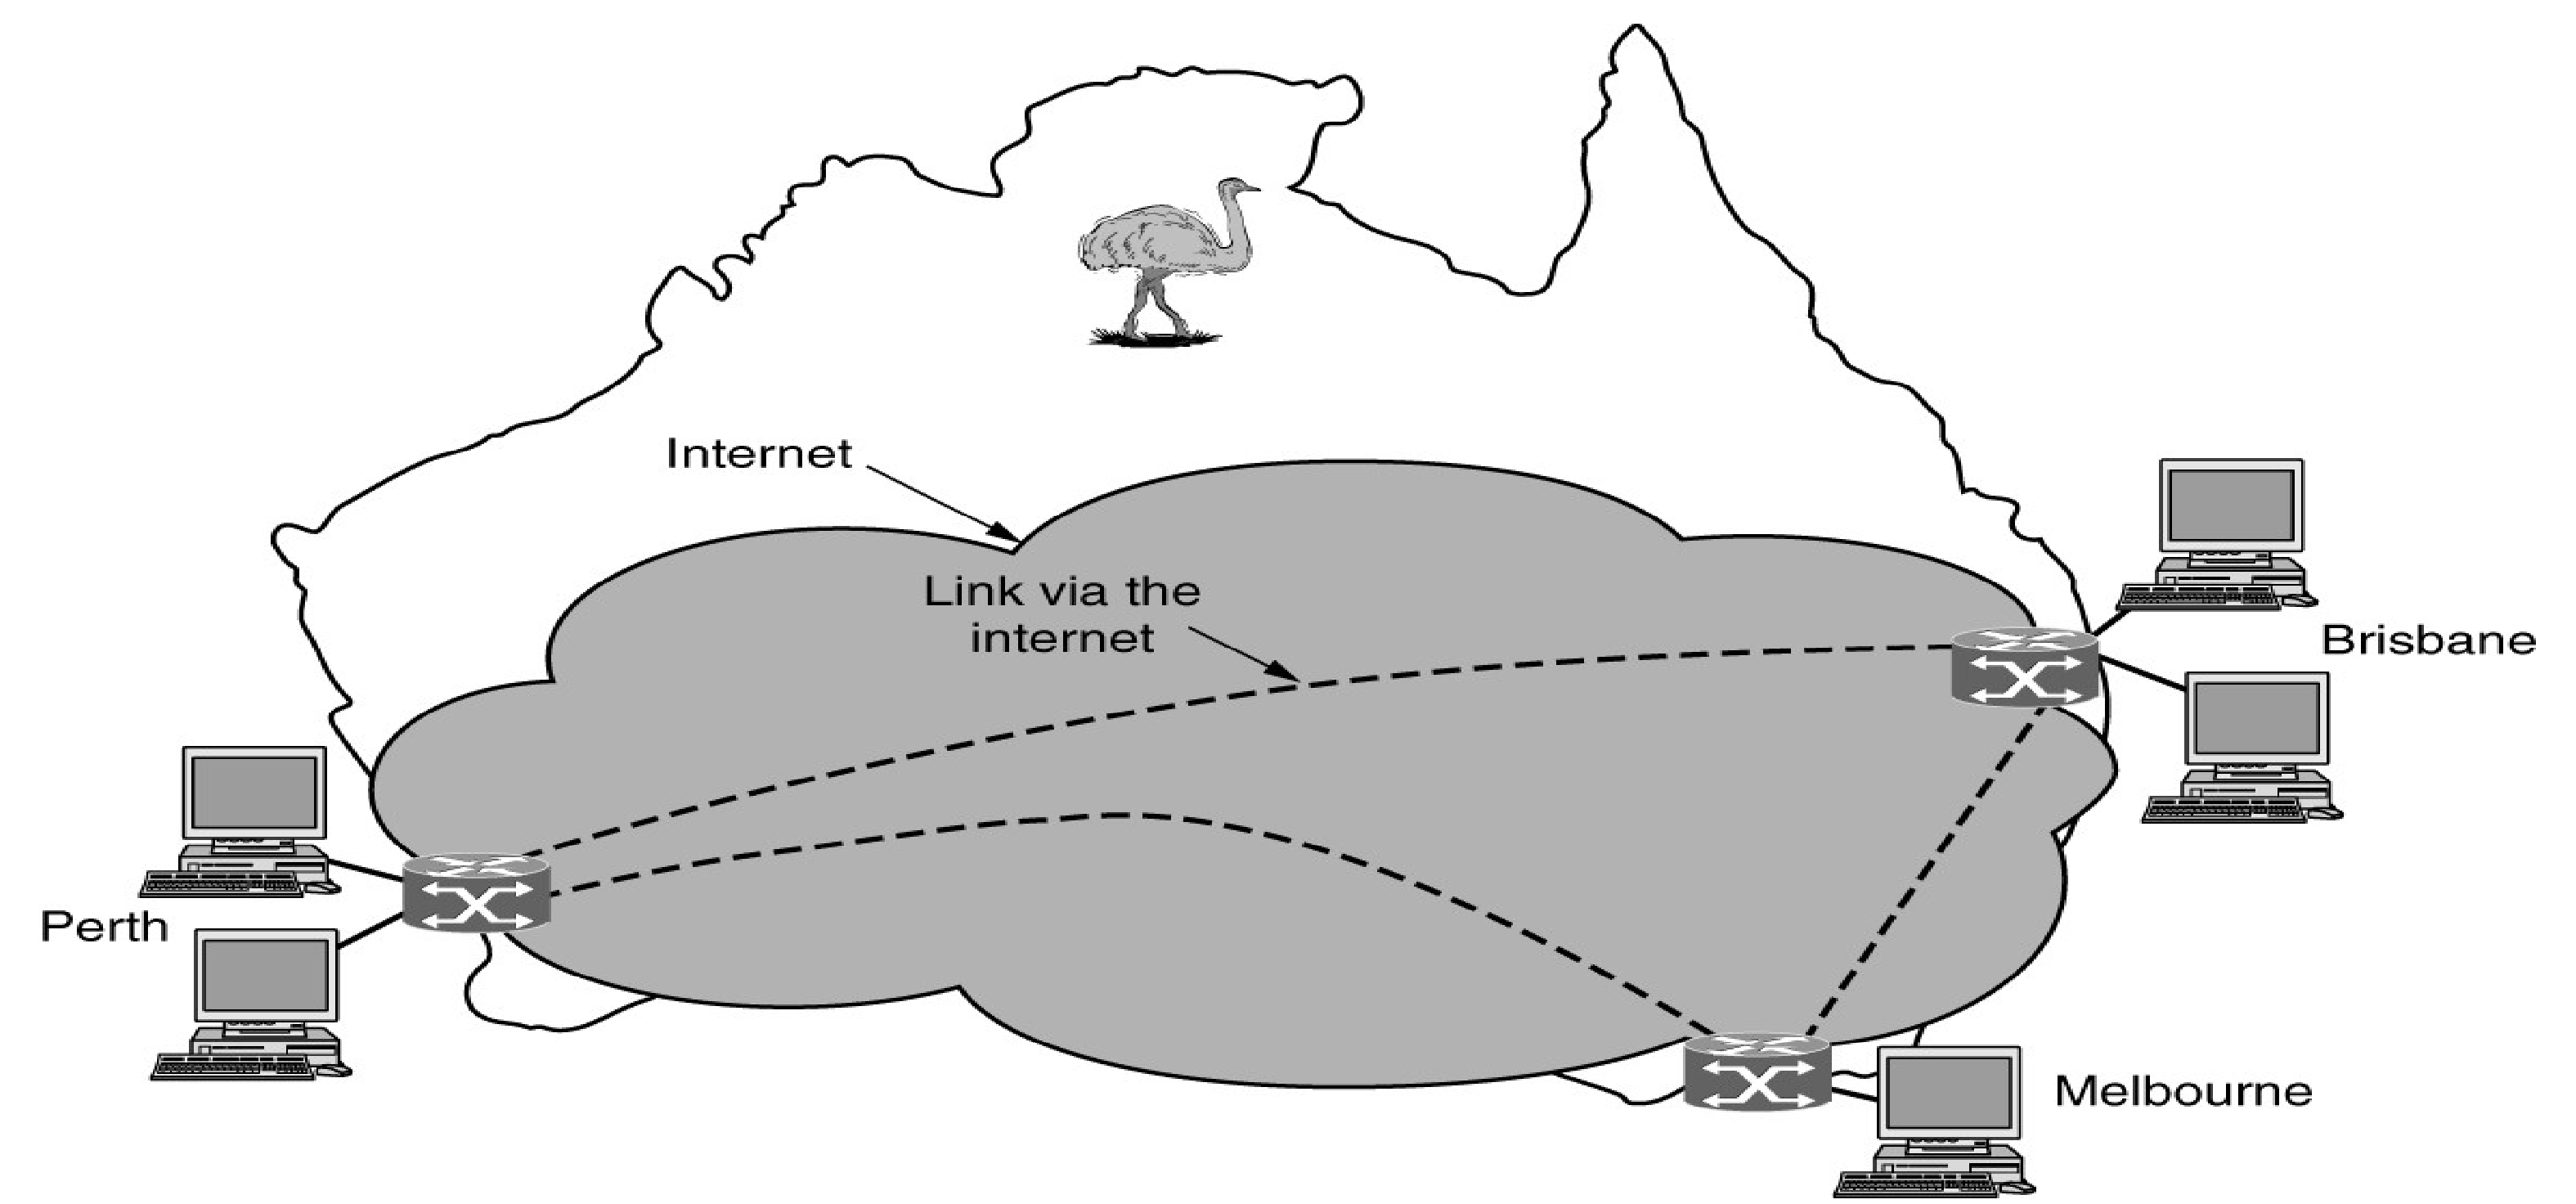
\includegraphics[width=0.55\linewidth]{cap01/wan_internet.png}
    \caption{La stessa WAN realizzata come rete privata virtuale (VPN) sopra Internet.}
\end{figure}

Invece di affittare linee, gli uffici si collegano con \textbf{collegamenti virtuali} che viaggiano
sopra la normale connettività Internet: per la WAN è come se esistesse una linea diretta tra le
sedi, ma in realtà i dati attraversano la rete di reti. È una \textbf{VPN} (\emph{Virtual Private
Network}). È \textbf{economica e flessibile}, ma la capacità \textbf{non è più nostra}: le prestazioni
seguono quello che sta facendo Internet in quel momento, senza garanzie di velocità né di
affidabilità.

\subsubsection*{3. Attraverso la rete di un ISP}

\begin{figure}[H]
    \centering
    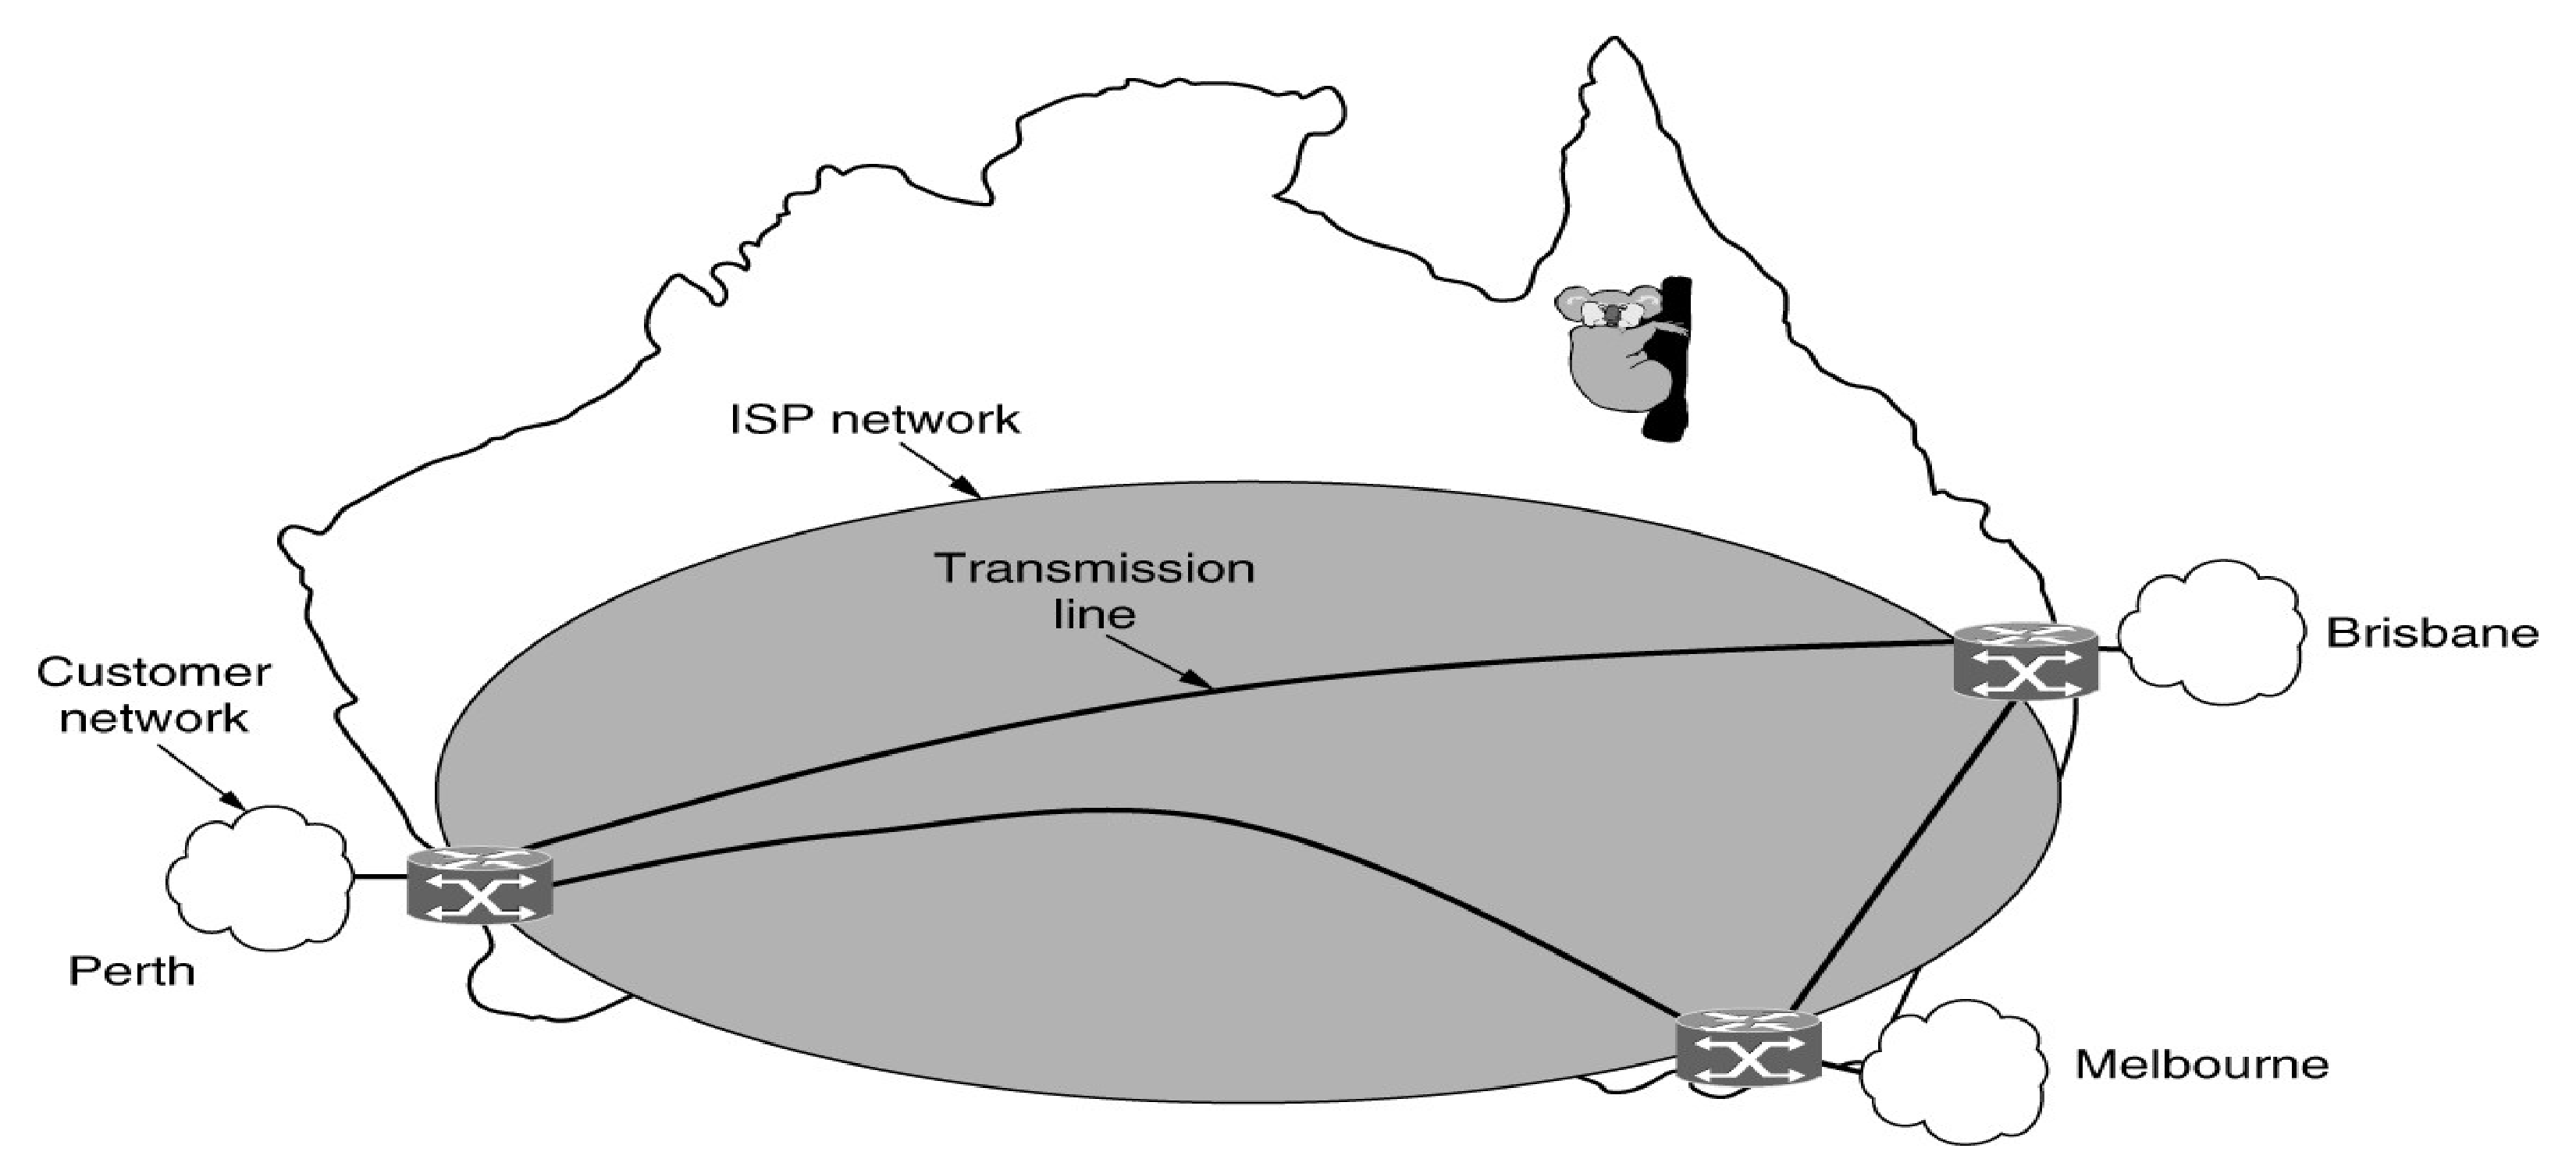
\includegraphics[width=0.55\linewidth]{cap01/wan_isp.png}
    \caption{Gli uffici collegati attraverso la rete di un ISP.}
\end{figure}

Le reti delle sedi si collegano a un \textbf{Internet Service Provider}, e la \textbf{rete dell'ISP}
trasporta il traffico tra le sedi e verso il resto di Internet. L'azienda non gestisce linee
proprie: se ne occupa l'ISP, che possiede o affitta le proprie dorsali (anche intercontinentali) e
offre il servizio secondo un contratto.

\begin{table}[H]
\centering
\begin{tabular}{p{3.2cm}p{3.5cm}p{3.5cm}p{3.5cm}}
\toprule
 & \textbf{Linee dedicate} & \textbf{VPN su Internet} & \textbf{Rete di un ISP} \\
\midrule
Chi gestisce le linee & l'azienda (affitta) & nessuno in particolare & l'ISP \\
Capacità garantita & sì & no & secondo contratto \\
Costo & alto & basso & medio \\
Flessibilità & bassa & alta & media \\
\bottomrule
\end{tabular}
\caption{I tre modi di realizzare una WAN.}
\end{table}

\subsection{WAN eterogenee e internetwork}

Una WAN grande raramente usa una sola tecnologia: nello stesso disegno convivono dorsali
commutate, collegamenti punto-punto, hub e LAN.

\begin{figure}[H]
    \centering
    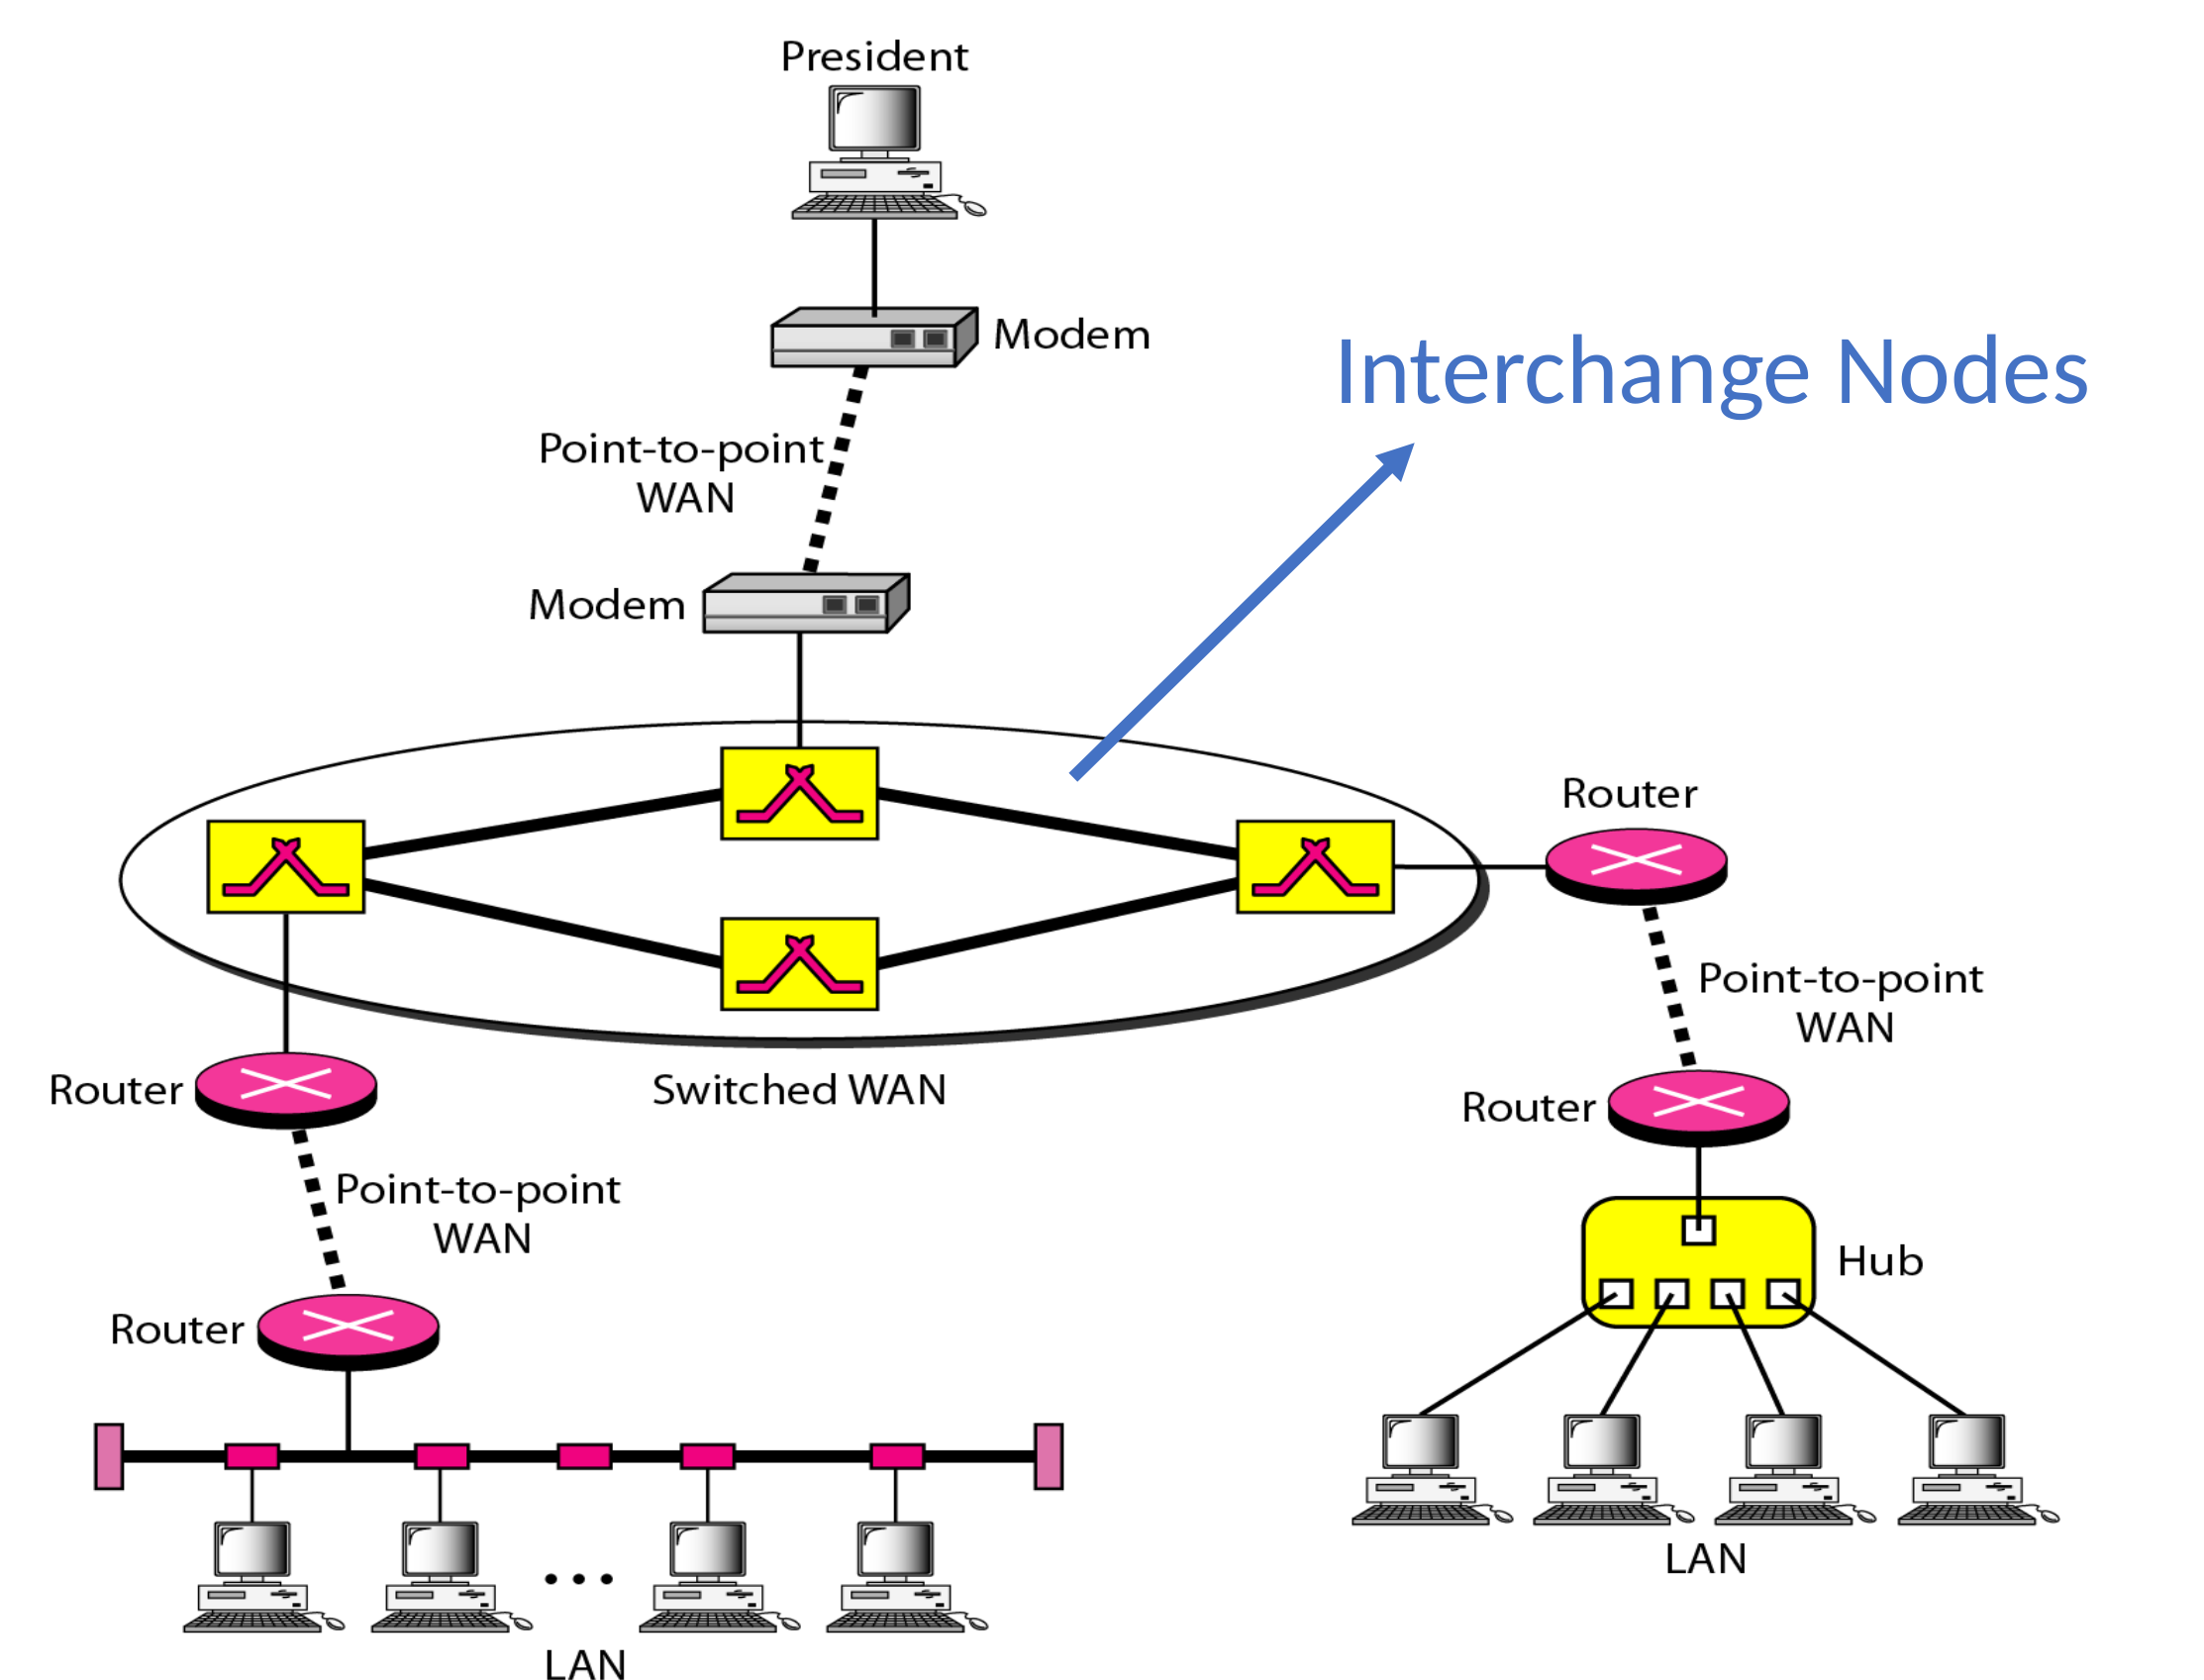
\includegraphics[width=0.55\linewidth]{cap01/wan_eterogenea.png}
    \caption{Una WAN eterogenea: WAN commutata, WAN punto-punto, LAN e i nodi di interscambio che le raccordano.}
\end{figure}

\dfn{Internetwork, gateway e router}{
    Un insieme di \textbf{reti distinte}, gestite in modo \textbf{indipendente} e collegate tra loro è
    una \textbf{internetwork}. Il dispositivo che unisce due reti di tipo diverso, e ``traduce'' tra
    loro, è un \textbf{gateway}; quando il gateway opera al livello di rete si chiama \textbf{router}.
}

% ══════════════════════════════════════════════════════════════
\section{Internet Service Provider}
% ══════════════════════════════════════════════════════════════

\dfn{Internet Service Provider (ISP)}{
    Un \textbf{ISP} è un'organizzazione che fornisce i servizi per \textbf{accedere}, usare o
    partecipare a Internet. Può essere commerciale, di proprietà di una comunità, no-profit, oppure
    privato (per esempio un'azienda o un'università).
}

\begin{figure}[H]
    \centering
    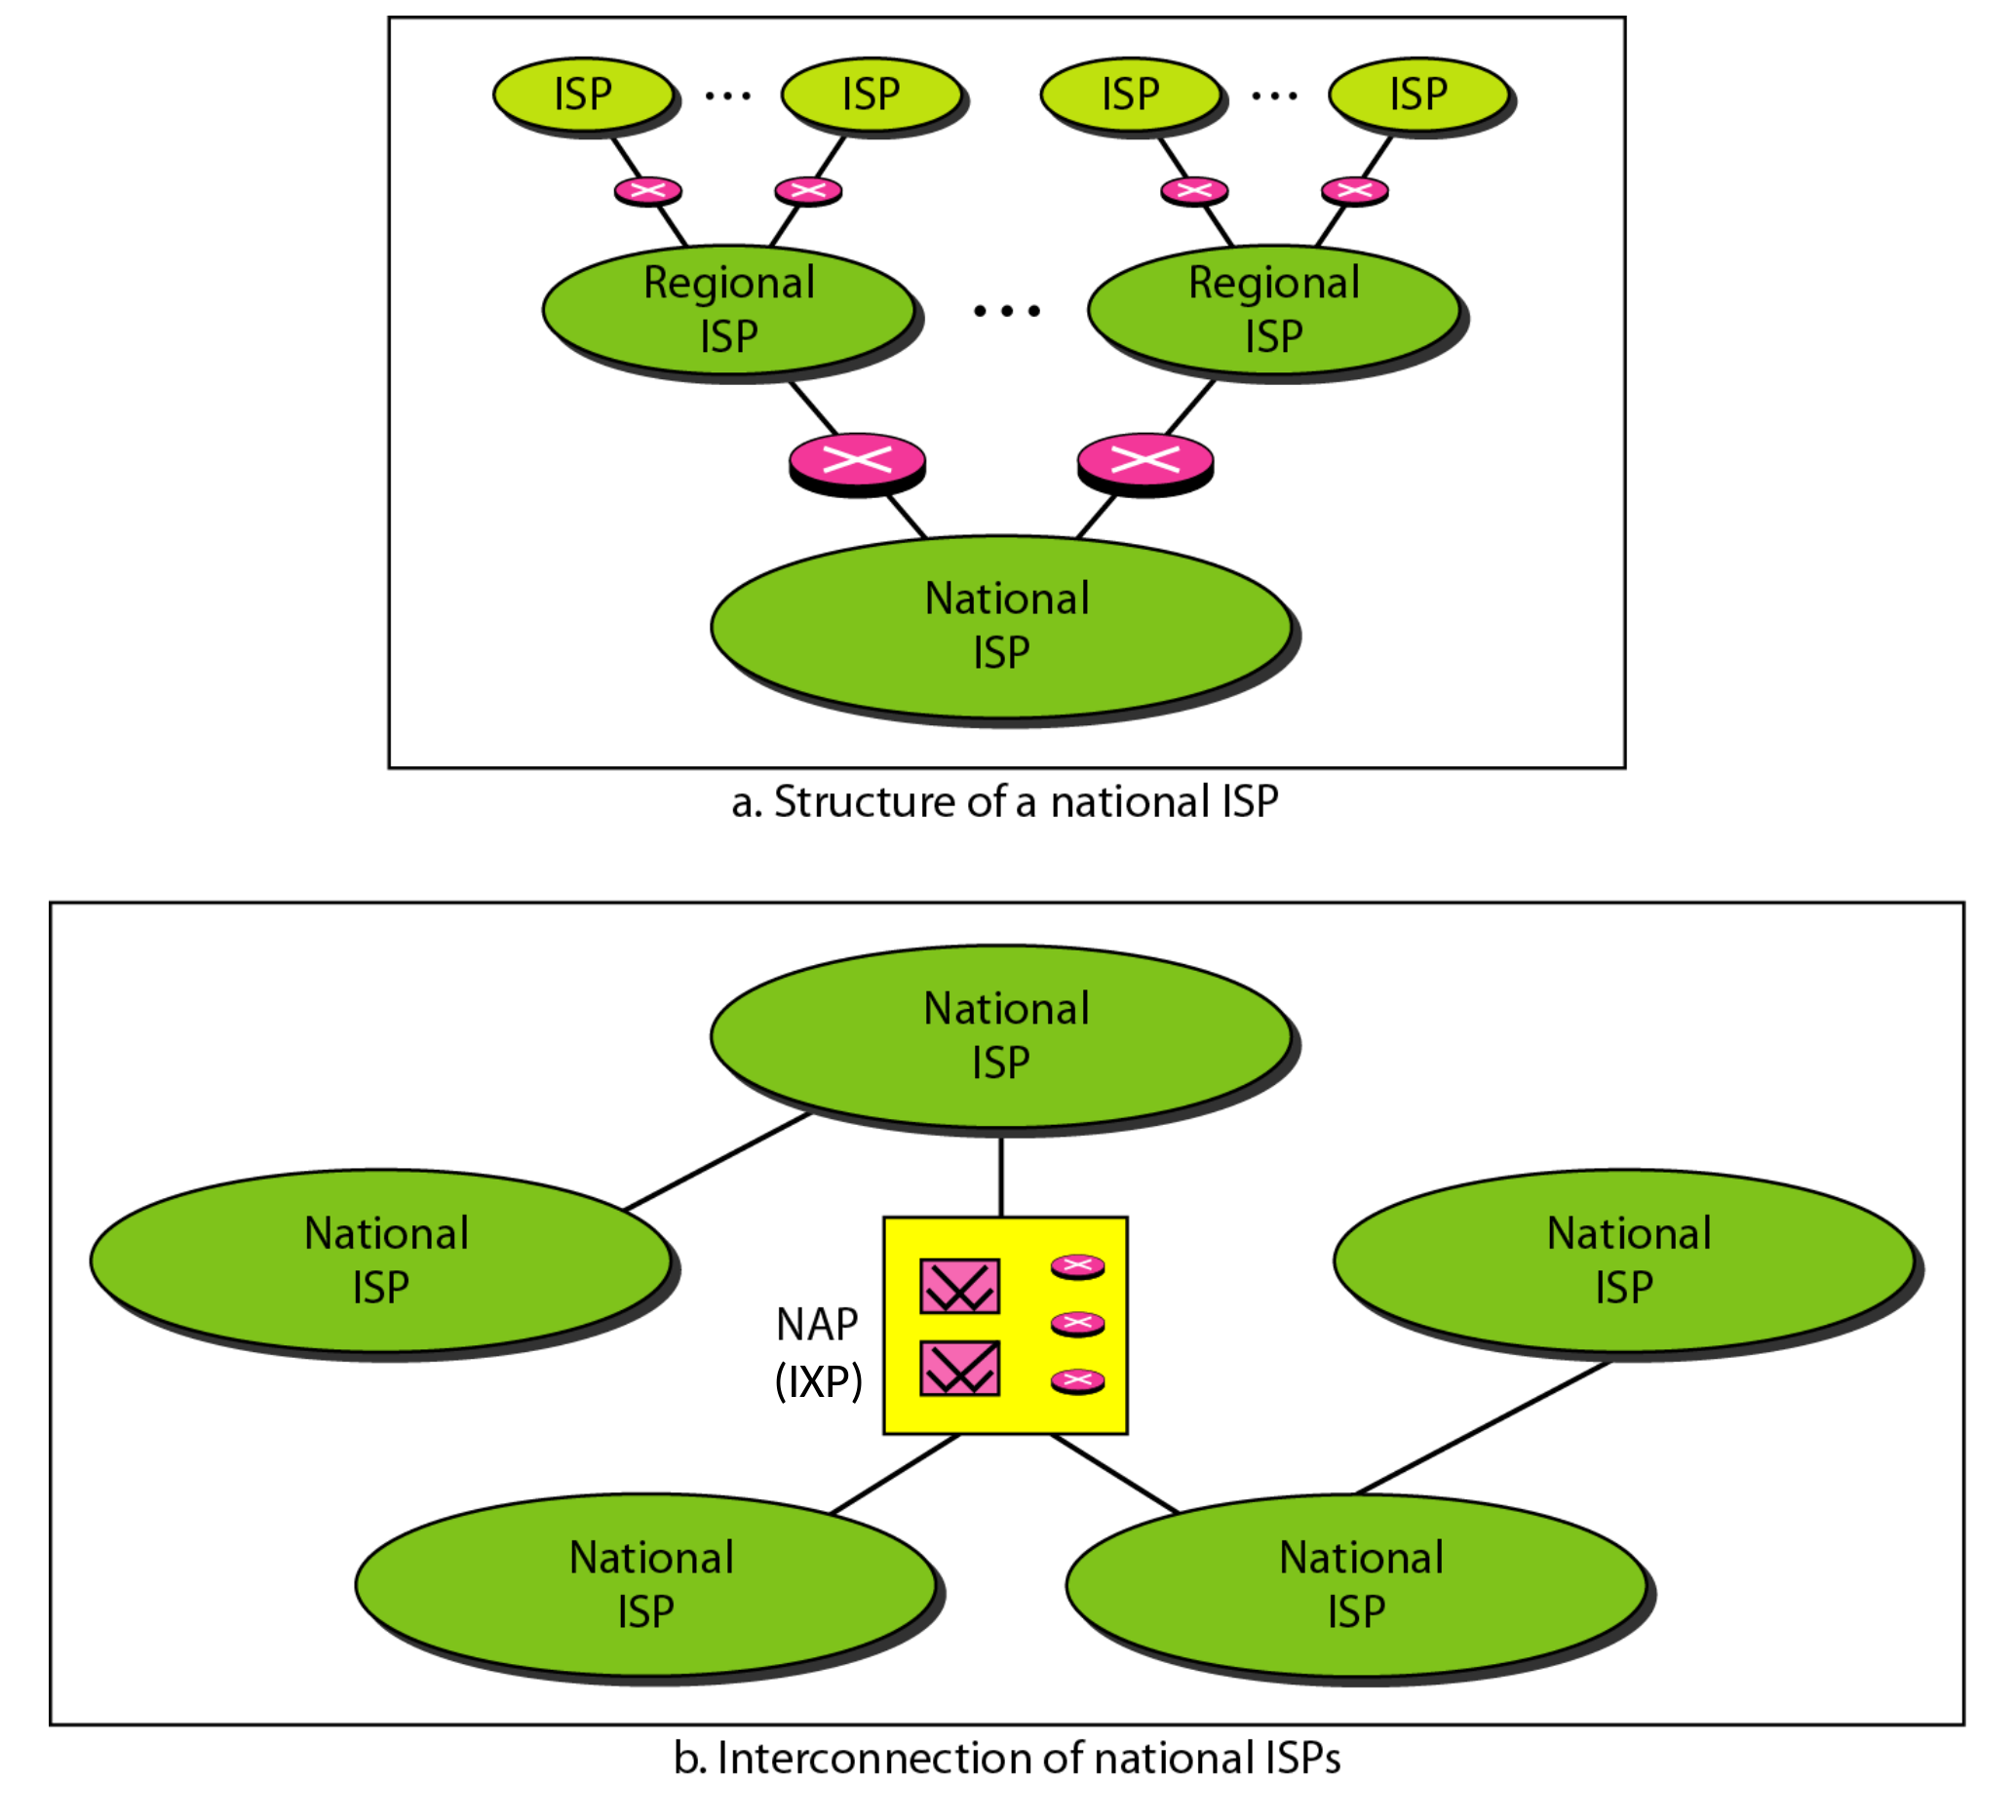
\includegraphics[width=0.45\linewidth]{cap01/isp_struttura.png}
    \caption{(a) Struttura di un ISP nazionale: ISP regionali e locali appesi a quello nazionale. (b) ISP nazionali interconnessi attraverso un NAP/IXP.}
\end{figure}

La rete di un ISP è organizzata in modo \textbf{gerarchico}:

\begin{itemize}
    \item un \textbf{PoP} (\emph{Point of Presence}) è il punto, uno o più router, in cui i clienti si
          collegano al fornitore: il vostro router di casa si collega a un PoP del vostro ISP, da cui
          partono collegamenti più capaci;
    \item gli \textbf{ISP di accesso} coprono aree locali;
    \item gli \textbf{ISP regionali} coprono aree più grandi;
    \item gli \textbf{ISP nazionali} coprono intere nazioni;
    \item gli ISP si scambiano traffico negli \textbf{IXP} (\emph{Internet Exchange Point}), detti anche
          \textbf{NAP} (\emph{Network Access Point}): punti di incontro, spesso gestiti da un soggetto
          terzo neutrale.
\end{itemize}

\subsection{Chi si collega con chi, e chi paga}

\begin{itemize}
    \item Collegare ogni ISP a ogni altro formerebbe una \textbf{full mesh}: con migliaia di ISP,
          servirebbero milioni di collegamenti. Impossibile.
    \item Quindi un ISP \textbf{cliente} paga un ISP \textbf{fornitore} per il transito del traffico, a
          ogni livello della gerarchia (l'ISP di accesso paga il regionale, il regionale paga il
          nazionale).
    \item Due ISP \textbf{allo stesso livello} possono invece fare \textbf{peering}: si collegano
          direttamente e si scambiano il traffico reciproco, di solito senza pagarsi.
    \item Un \textbf{IXP} è un edificio con l'hardware necessario perché molti ISP facciano peering
          contemporaneamente.
    \item Un ISP può fare \textbf{multi-homing}: comprare connettività da due fornitori diversi, così
          da continuare a funzionare se uno dei due si guasta.
\end{itemize}

\begin{figure}[H]
\centering
\begin{tikzpicture}[every node/.style={font=\scriptsize\sffamily},
  isp/.style={ellipse, draw=netblue!70, fill=cloudbg, minimum width=2.2cm, minimum height=0.8cm, align=center},
  ixp/.style={rectangle, rounded corners=2pt, draw=netorange, fill=netorange!20, minimum width=1cm, minimum height=0.55cm, align=center}]
  \node[isp, fill=netblue!30] (t1a) at (-3,3) {ISP globale A};
  \node[isp, fill=netblue!30] (t1b) at (3,3) {ISP globale B};
  \node[ixp] (ixp1) at (0,3) {IXP};
  \node[isp] (ra) at (-4.5,1.2) {ISP regionale};
  \node[isp] (rb) at (-1.2,1.2) {ISP regionale};
  \node[isp] (rc) at (3.2,1.2) {ISP regionale};
  \node[ixp] (ixp2) at (-2.85,0.2) {IXP};
  \node[isp] (a1) at (-5.5,-0.8) {accesso};
  \node[isp] (a2) at (-3.3,-1.1) {accesso};
  \node[isp] (a3) at (-0.8,-0.8) {accesso};
  \node[isp] (a4) at (2.2,-0.8) {accesso};
  \node[isp] (a5) at (4.6,-0.8) {accesso};
  \node[isp, draw=netgreen!70!black, fill=netgreen!15, minimum width=3cm] (cp) at (6.2,2.2) {rete privata del\\content provider};
  \foreach \c/\p in {ra/t1a, rb/t1a, rb/t1b, rc/t1b, a1/ra, a2/ra, a3/rb, a4/rc, a5/rc}
     \draw[-{Stealth}, thick, netblue] (\c) -- (\p);
  \draw[thick, netorange, dashed] (t1a) -- (ixp1) -- (t1b);
  \draw[thick, netorange, dashed] (ra) -- (ixp2) -- (rb);
  \draw[thick, netgreen!70!black, dashed] (cp) -- (a5); \draw[thick, netgreen!70!black, dashed] (cp) -- (a4); \draw[thick, netgreen!70!black, dashed] (cp) -- (t1b);
  \draw[-{Stealth}, thick, netblue] (-6.8,-2) -- ++(0.8,0) node[right] {cliente $\rightarrow$ fornitore (il cliente paga)};
  \draw[thick, netorange, dashed] (-1.6,-2) -- ++(0.8,0) node[right] {peering (di solito gratuito)};
  \draw[thick, netgreen!70!black, dashed] (2.6,-2) -- ++(0.8,0) node[right] {peering del content provider};
  \node[lbl, text=netblue] at (0.2,1.95) {multi-homing:\\\scriptsize due fornitori};
\end{tikzpicture}
\caption{La struttura economica di Internet: gerarchia di clienti e fornitori, peering negli IXP e reti private dei content provider.}
\end{figure}

\info{I content provider}{
    I grandi fornitori di contenuti (Google, Netflix, Meta, \dots) costruiscono \textbf{reti private
    globali} e fanno peering \textbf{direttamente con gli ISP di livello basso}, scavalcando i livelli
    superiori. Così spendono meno (non pagano il transito) e controllano direttamente come i loro
    contenuti arrivano agli utenti.
}

% ══════════════════════════════════════════════════════════════
\section{Collegarsi a un ISP}
% ══════════════════════════════════════════════════════════════

\begin{figure}[H]
    \centering
    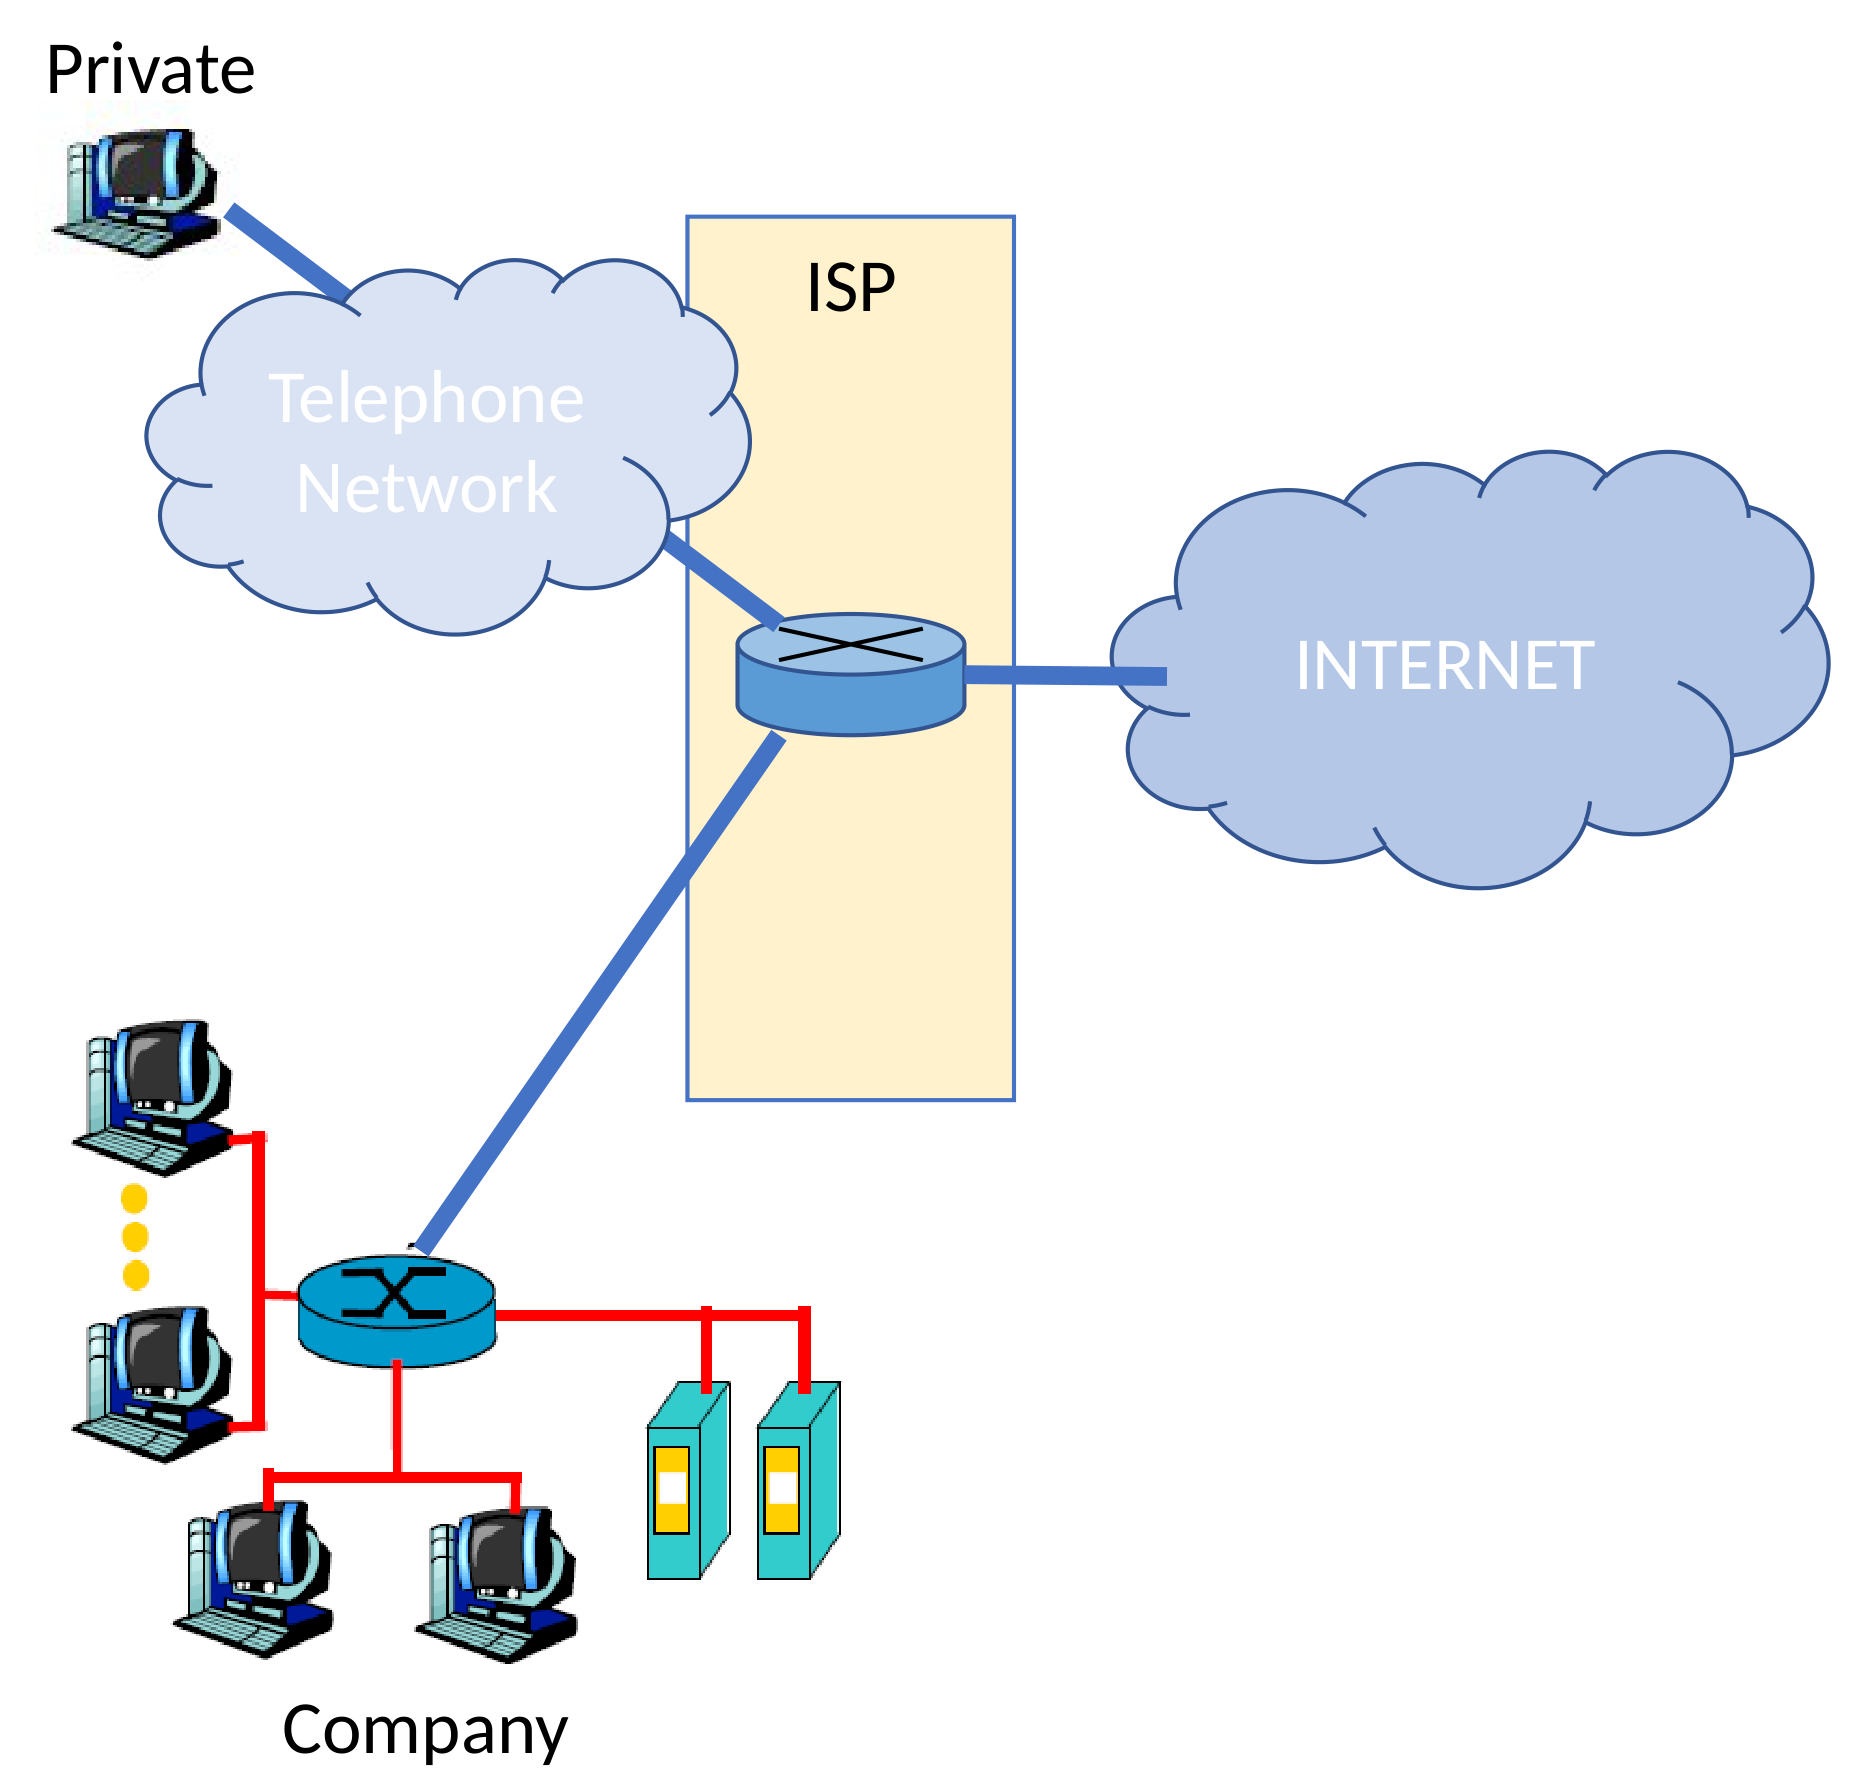
\includegraphics[width=0.45\linewidth]{cap01/connessione_isp.png}
    \caption{In alto una connessione privata attraverso la rete telefonica; in basso un'azienda con un collegamento dedicato all'ISP.}
\end{figure}

\begin{itemize}
    \item \textbf{Accesso residenziale}: un \textbf{modem} (o un \textbf{ONT}, per la fibra) raggiunge
          il fornitore sfruttando l'infrastruttura esistente, cioè la rete telefonica o quella via cavo.
    \item \textbf{Accesso aziendale}: un'azienda medio-grande ha molto più traffico, quindi compra un
          \textbf{collegamento dedicato} direttamente verso l'ISP e collega la propria rete dietro un
          \textbf{router} aziendale, che dialoga con un router dell'ISP.
\end{itemize}

\begin{figure}[H]
\centering
\begin{tikzpicture}[every node/.style={font=\scriptsize\sffamily}]
  \node (l) at (0,0.7) {\icon[0.8cm]{laptop}};
  \node (s) at (0,-0.7) {\icon[0.6cm]{smartphone}};
  \node (r) at (2.6,0) {\icon[1.1cm]{accesspoint}};
  \node[below=-2pt of r] {router di casa};
  \node[box, fill=lphy!40, minimum width=1.6cm, font=\scriptsize\sffamily] (m) at (5.0,0) {modem\\o ONT};
  \node[box, fill=cloudbg, minimum width=1.8cm, font=\scriptsize\sffamily] (pop) at (10.4,0) {PoP\\dell'ISP};
  \node[netcloud, minimum width=2.4cm] (inet) at (13.6,0) {Internet};
  \draw[wireless] (l) -- (r); \draw[wireless] (s) -- (r);
  \draw[wired] (r) -- (m);
  \draw[wired, netorange, line width=1.8pt] (m) -- node[above, lbl] {rete di accesso} node[below, lbl] {doppino, cavo, fibra, 5G} (pop);
  \draw[wired, line width=2.5pt] (pop) -- (inet);
  \draw[decorate, decoration={brace, amplitude=6pt}] (-0.5,1.5) -- (5.9,1.5) node[midway, above=7pt] {la vostra rete (LAN)};
  \draw[decorate, decoration={brace, amplitude=6pt}] (6.1,1.5) -- (14.9,1.5) node[midway, above=7pt] {di qualcun altro};
\end{tikzpicture}
\caption{Il percorso da casa a Internet: il primo salto fuori da casa appartiene già all'ISP.}
\end{figure}

In entrambi i casi, \textbf{il primo salto fuori dall'edificio appartiene a qualcun altro}: subito
fuori dalla rete di casa o dell'azienda c'è un ISP, che va pagato per i servizi che fornisce.

\subsection{Tecnologie di accesso residenziale}

\begin{table}[H]
\centering
\begin{tabular}{p{2.7cm}p{5cm}p{6.3cm}}
\toprule
\textbf{Tecnologia} & \textbf{Su cosa viaggia} & \textbf{Da ricordare} \\
\midrule
DSL / ADSL & il doppino telefonico esistente & la velocità \textbf{cala con la distanza} dalla centrale \\
Cavo (HFC) & fibra fino alla strada, cavo coassiale fino in casa & l'ultimo tratto è \textbf{condiviso} con i vicini \\
FTTH & fibra fino in casa, ONT in casa & centinaia di Mb/s, fino al gigabit e oltre \\
Wireless fisso & radio 5G da una stazione base & nessun cavo da posare \\
\bottomrule
\end{tabular}
\caption{Le tecnologie di accesso residenziale oggi.}
\end{table}

\begin{itemize}
    \item Sono tutte \textbf{asimmetriche}: la velocità in \emph{download} (verso casa) è maggiore di
          quella in \emph{upload} (verso Internet), perché da casa si scarica molto più di quanto si invii.
    \item Le cifre pubblicizzate sono un \textbf{tetto}; e su un mezzo condiviso, quel tetto è condiviso.
    \item Nella fibra non c'è (de)modulazione del segnale come nel modem tradizionale: per questo
          l'apparecchio si chiama \textbf{ONT} (\emph{Optical Network Terminal}) e non modem.
\end{itemize}

\info{Un po' di storia delle velocità di accesso}{
    \begin{tabular}{ll}
    Modem analogico & 56 kb/s \\
    ISDN (\emph{Integrated Services Digital Network}) & 128 kb/s \\
    ADSL (\emph{Asymmetric Digital Subscriber Line}) & da 1 a 20 Mb/s \\
    Doppino in rame di nuova generazione & da 10 a 100 Mb/s \\
    Fibra ottica (tramite ONT) & da 50 Mb/s a decine di Gb/s \\
    \end{tabular}
}

% ══════════════════════════════════════════════════════════════
\section{Riepilogo}
% ══════════════════════════════════════════════════════════════

\riepilogo{
\begin{itemize}
    \item Una rete è una collezione di dispositivi \textbf{autonomi} che possono \textbf{scambiarsi
          informazione}: \textbf{host} ai bordi, \textbf{commutatori di pacchetto} (router e switch) in mezzo.
    \item Comunicano \textbf{processi}: un client chiede, un server risponde; nel P2P ogni peer fa entrambe le cose.
    \item \textbf{Internet} è una rete di reti indipendenti, integrate attraverso gli ISP e tenute insieme da \textbf{IP}.
    \item I dati viaggiano in \textbf{pacchetti}, memorizzati e inoltrati (\emph{store-and-forward}),
          che si accodano quando il collegamento è occupato e vengono persi quando la coda è piena.
    \item Internet usa la \textbf{commutazione di pacchetto} perché il traffico è a raffica.
    \item La \textbf{topologia} dice chi è collegato con chi; la \textbf{scala} dice se la rete è PAN, LAN, MAN o WAN.
    \item Gli ISP formano una gerarchia di clienti e fornitori, con \textbf{peering} negli IXP.
\end{itemize}
}

Una sola richiesta Web attraversa decine di queste reti, con tecnologie e gestori diversi. Come
si tiene sotto controllo una tale complessità? La risposta è l'argomento del prossimo capitolo:
la \textbf{stratificazione}.
   % Lezione 01
  \chapter{Stratificazione, modelli di riferimento e incapsulamento}

Questo è forse il capitolo più importante di tutto il corso: introduce il \textbf{modello a
strati}, la chiave di lettura di tutto ciò che verrà dopo. Ogni parte successiva della dispensa si
occuperà di uno strato preciso.

% ══════════════════════════════════════════════════════════════
\section{Il Web è un'applicazione}
% ══════════════════════════════════════════════════════════════

Partiamo da un chiarimento: \textbf{il Web non è Internet}. Il Web è \emph{una} delle applicazioni
che girano sopra Internet; la posta elettronica, lo streaming, la messaggistica, il trasferimento di
file e i giochi sono altre applicazioni, e ciascuna chiede alla rete qualcosa di leggermente diverso.
Nel capitolo precedente abbiamo visto di cosa è fatta una rete e come i pezzi sono collegati. Ora
la domanda è:

\begin{center}
\large\itshape Che cosa deve esistere, e funzionare, perché una pagina compaia nel browser?
\end{center}

La risposta a questa domanda è la struttura di tutto il resto del corso.

\subsection{Cosa attraversa una singola richiesta HTTP}

Un browser sull'host A chiede una pagina al server Web B. Tra i due c'è un bel po' di roba:

\begin{figure}[H]
\centering
\begin{tikzpicture}[every node/.style={font=\footnotesize\sffamily}]
  \node (A) at (0,0) {\icon[1.2cm]{pc}};
  \node[below=-2pt of A] {A (browser)};
  \node (R) at (3.6,0) {\icon[1.4cm]{router}};
  \node[below=0pt of R] {router di casa};
  \node[box, fill=cloudbg, minimum width=1.4cm] (isp) at (8,0) {ISP};
  \node[netcloud, minimum width=3.2cm, minimum height=1.8cm] (inet) at (10.2,-2.5) {Internet};
  \node (B) at (13.3,-2.5) {\icon[0.8cm]{server}};
  \node[below=-2pt of B] {B (server Web)};
  \draw[wired] (A) -- node[above, lbl] {cavo Ethernet} (R);
  \draw[wired, netorange, line width=1.6pt] (R) -- node[above, lbl, text=netorange] {doppino telefonico} node[below, lbl, text=netorange] {e rete telefonica} (isp);
  \draw[wired, line width=2pt] (isp) -- (inet);
  \draw[wired, line width=2pt] (inet) -- (B);
  \draw[msg, netred, dashed] (0.3,1.0) .. controls (5,2.6) and (11,2.2) .. node[pos=0.45, above, lbl, text=netred] {richiesta HTTP di A verso B} (13,-1.6);
\end{tikzpicture}
\caption{Una richiesta HTTP attraversa mezzi diversi, apparati diversi e una maglia di reti di cui nessuno dei soggetti coinvolti conosce l'interno.}
\end{figure}

\begin{itemize}
    \item Ogni apparato sul cammino è \textbf{hardware più software}, costruito da un produttore diverso.
    \item Ogni tratto è un \textbf{mezzo diverso}, con i propri errori e la propria velocità.
    \item Nessuno può progettare, o anche solo descrivere, un sistema del genere \textbf{tutto in una volta}.
\end{itemize}

\dfn{Divide et impera}{
    Si spezza il sistema complesso in \textbf{sottosistemi}, ciascuno con un compito proprio e un
    modo ben definito di chiedere aiuto al successivo; poi si progetta un sottosistema alla volta.
    Nelle reti questa scomposizione ha un nome: \textbf{stratificazione} (\emph{layering}).
}

% ══════════════════════════════════════════════════════════════
\section{Internet vista “dai bulloni” e come servizio}
% ══════════════════════════════════════════════════════════════

Prima di entrare negli strati, ricapitoliamo i due modi complementari di guardare Internet.

\subsection{La vista “nuts and bolts”}

Dal punto di vista dei suoi componenti fisici (i ``dadi e bulloni''), Internet è fatta di:

\begin{itemize}
    \item \textbf{miliardi di dispositivi di calcolo} connessi, gli \textbf{host} o \emph{end system},
          che eseguono applicazioni di rete e stanno ai \textbf{bordi} (\emph{edge}) di Internet;
    \item \textbf{commutatori di pacchetto} (\emph{packet switch}), che inoltrano pacchetti (blocchi di
          dati): router e switch;
    \item \textbf{collegamenti di comunicazione}: fibra, rame, radio, satellite, ciascuno con il
          proprio \emph{transmission rate};
    \item \textbf{reti}: collezioni di dispositivi, router e collegamenti gestite da una singola organizzazione.
\end{itemize}

\begin{figure}[H]
    \centering
    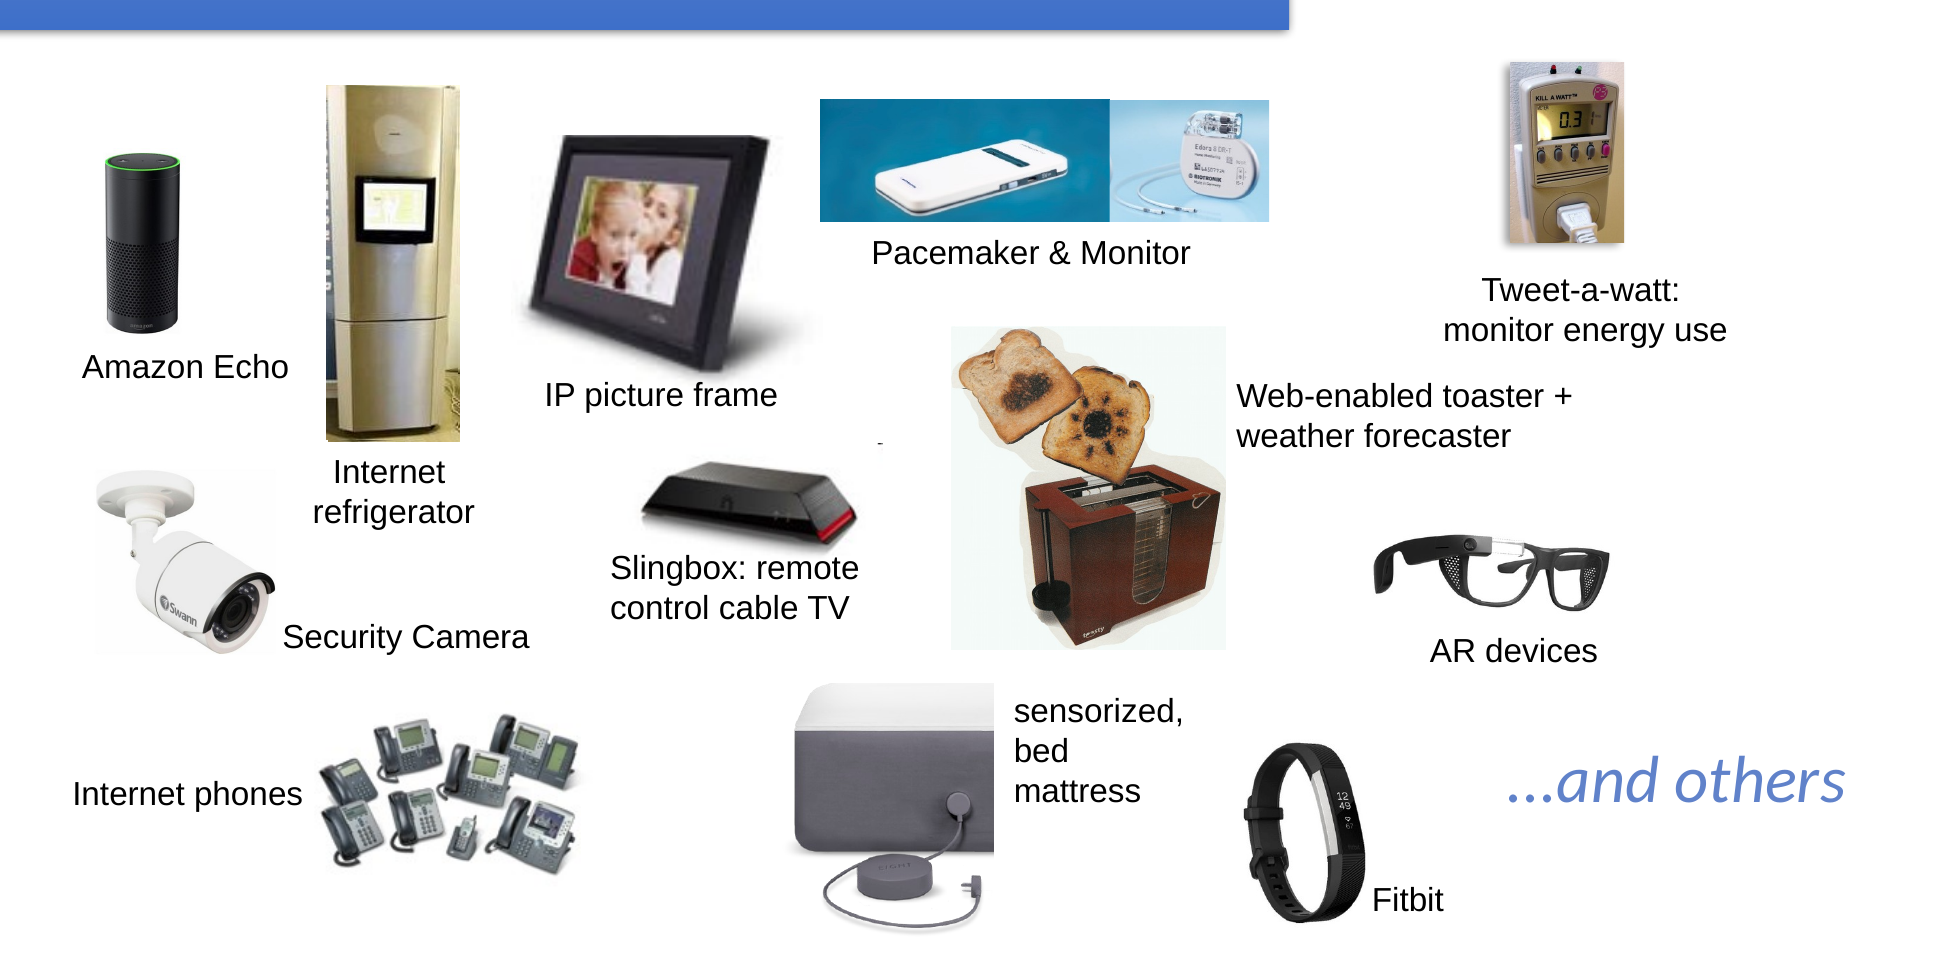
\includegraphics[width=0.72\linewidth]{cap02/dispositivi_iot.png}
    \caption{Non solo computer: frigoriferi, cornici digitali, telecamere, pacemaker, materassi sensorizzati, orologi\dots{} sono tutti host di Internet.}
\end{figure}

In questa vista i \textbf{protocolli sono ovunque}: controllano l'invio e la ricezione dei messaggi
(HTTP per il Web, TCP, IP, Wi-Fi, 4G, Ethernet, i protocolli proprietari di Skype, \dots).

\subsection{Internet come infrastruttura di servizi}

\begin{figure}[H]
\centering
\begin{minipage}{0.42\linewidth}\centering
  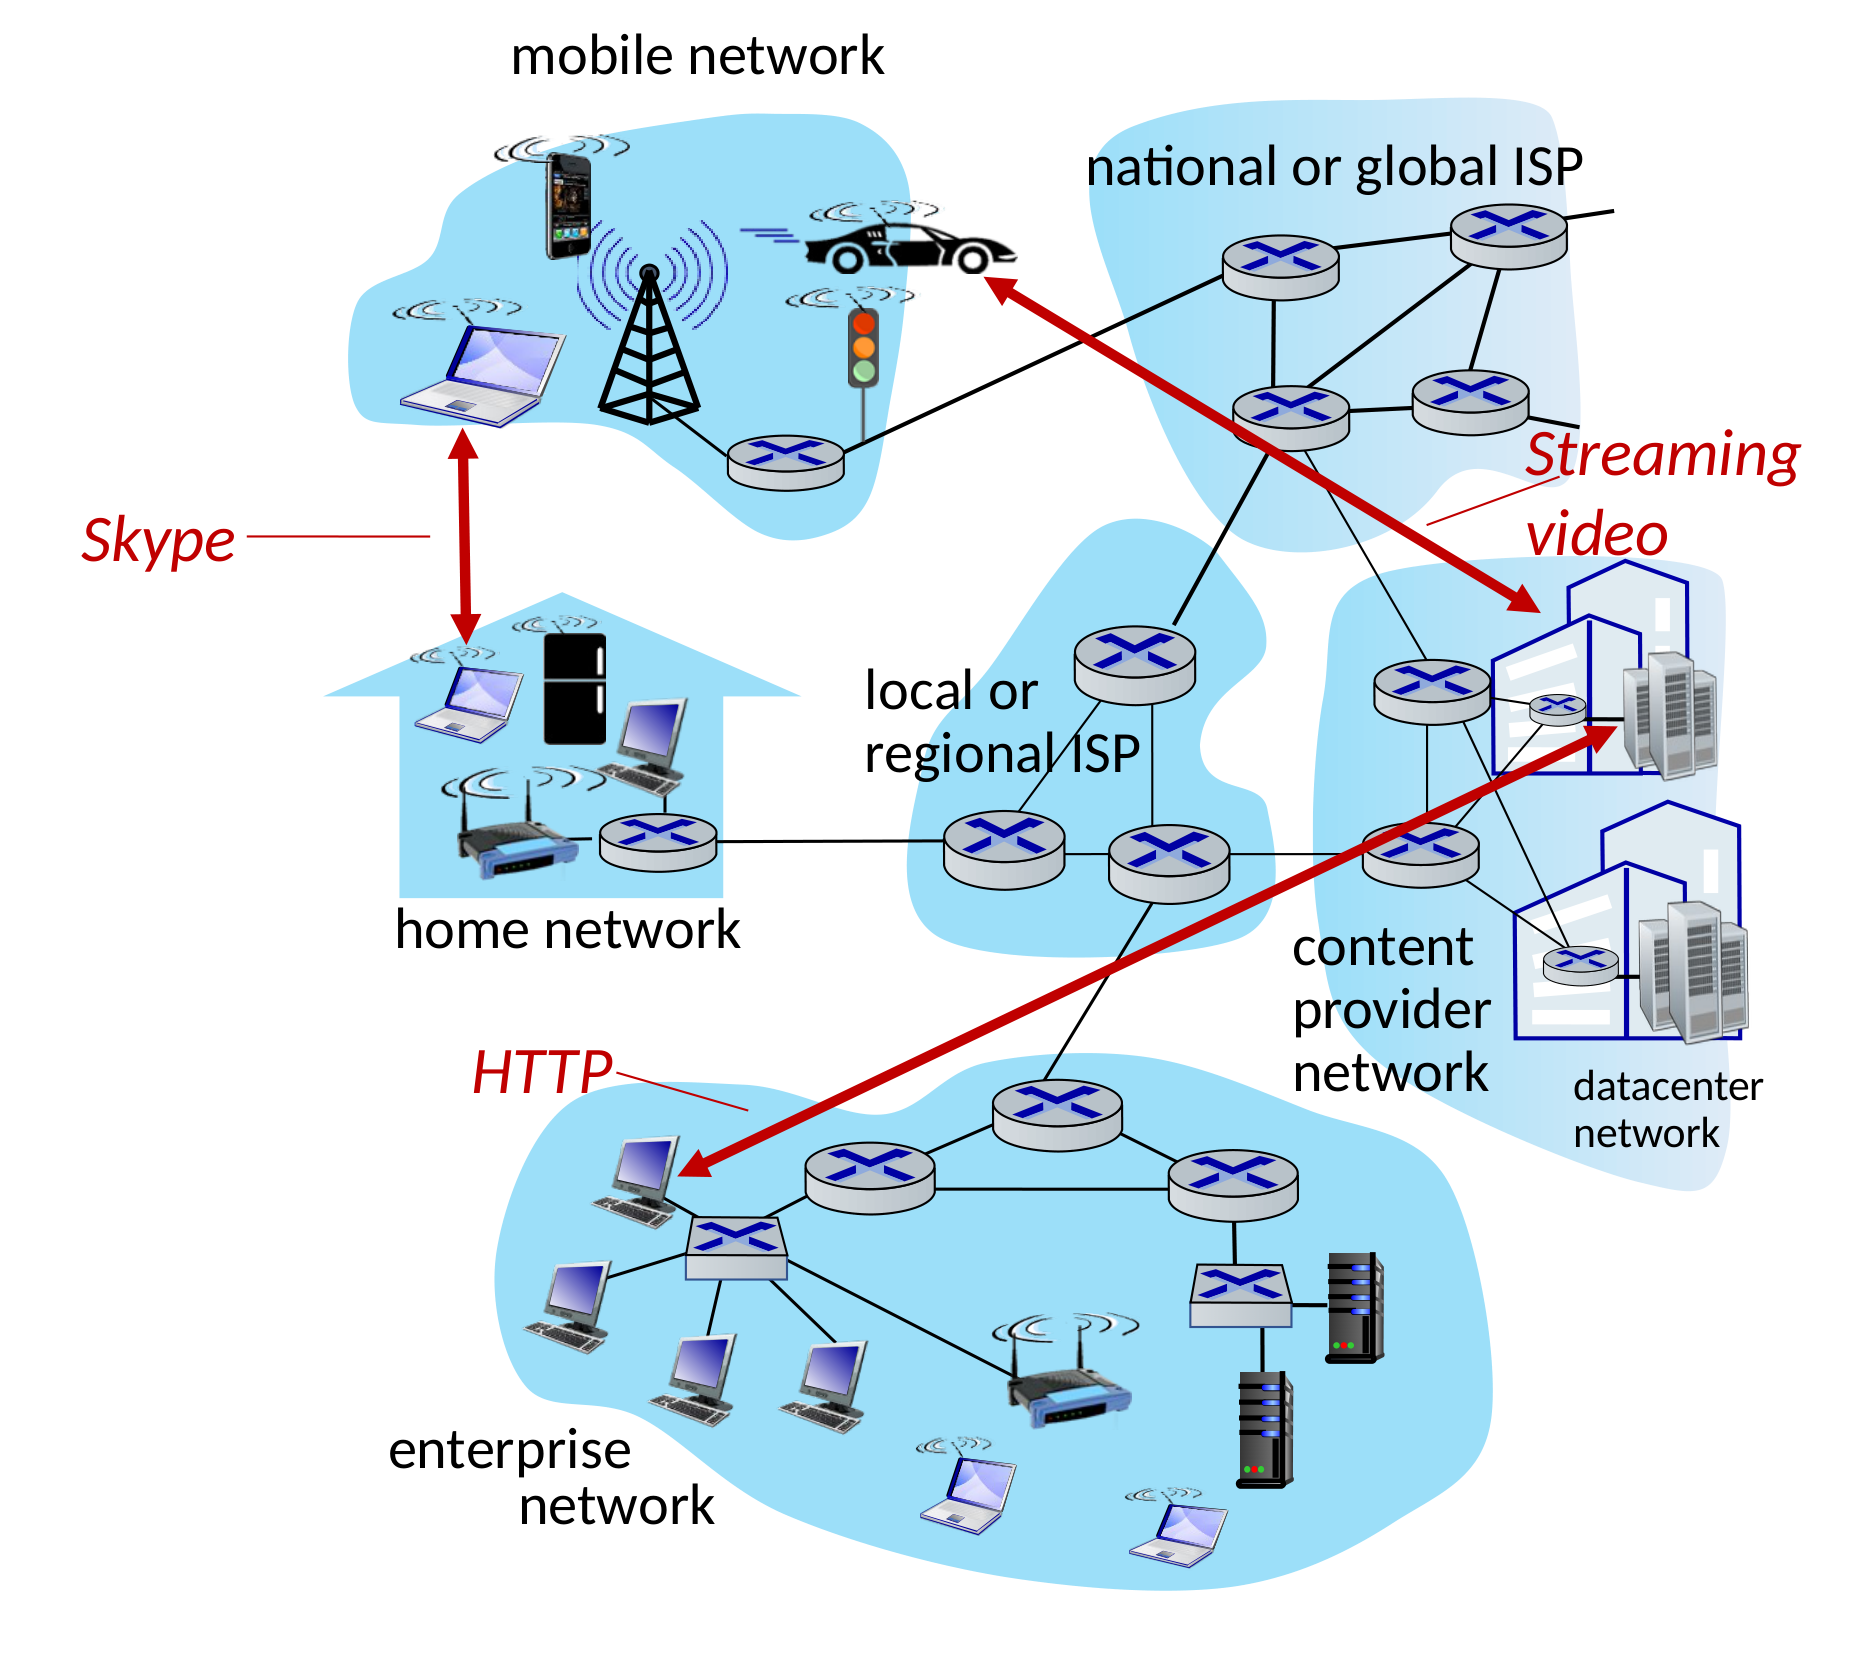
\includegraphics[width=\linewidth]{cap02/internet_servizi.png}
\end{minipage}\hfill
\begin{minipage}{0.54\linewidth}
Vista dall'alto, Internet non è fatta di cavi: è un'\textbf{infrastruttura che fornisce servizi alle
applicazioni} (Web, video, posta, videoconferenza, commercio elettronico, social media, elettrodomestici
connessi).
\begin{itemize}
  \item Fornisce anche un'\textbf{interfaccia di programmazione}: i ``ganci'' (\emph{hooks}) con cui
        un'applicazione si aggancia a Internet per inviare e ricevere dati.
  \item Come il servizio postale (posta ordinaria, raccomandata, espresso), offre \textbf{opzioni di
        servizio}: veloce o economico, garantito o no.
\end{itemize}
Sono proprio quei ganci che programmeremo, in C, con i socket.
\end{minipage}
\caption{Protocolli e servizi in azione sulla rete di reti.}
\end{figure}

\info{L'applicazione vede solo un servizio}{
    Le applicazioni non devono preoccuparsi di come i dati attraversano la rete: il flusso dei dati
    viene offerto loro \textbf{come servizio} dallo strato inferiore (il trasporto). È esattamente
    questo il senso della stratificazione.
}

% ══════════════════════════════════════════════════════════════
\section{Protocolli e standard}
% ══════════════════════════════════════════════════════════════

Ricordiamo la definizione del capitolo precedente: un \textbf{protocollo} fissa il \textbf{formato}
e l'\textbf{ordine} dei messaggi, e le \textbf{azioni} da compiere quando un messaggio viene inviato o
ricevuto. Vale per le persone come per le macchine.

\begin{figure}[H]
    \centering
    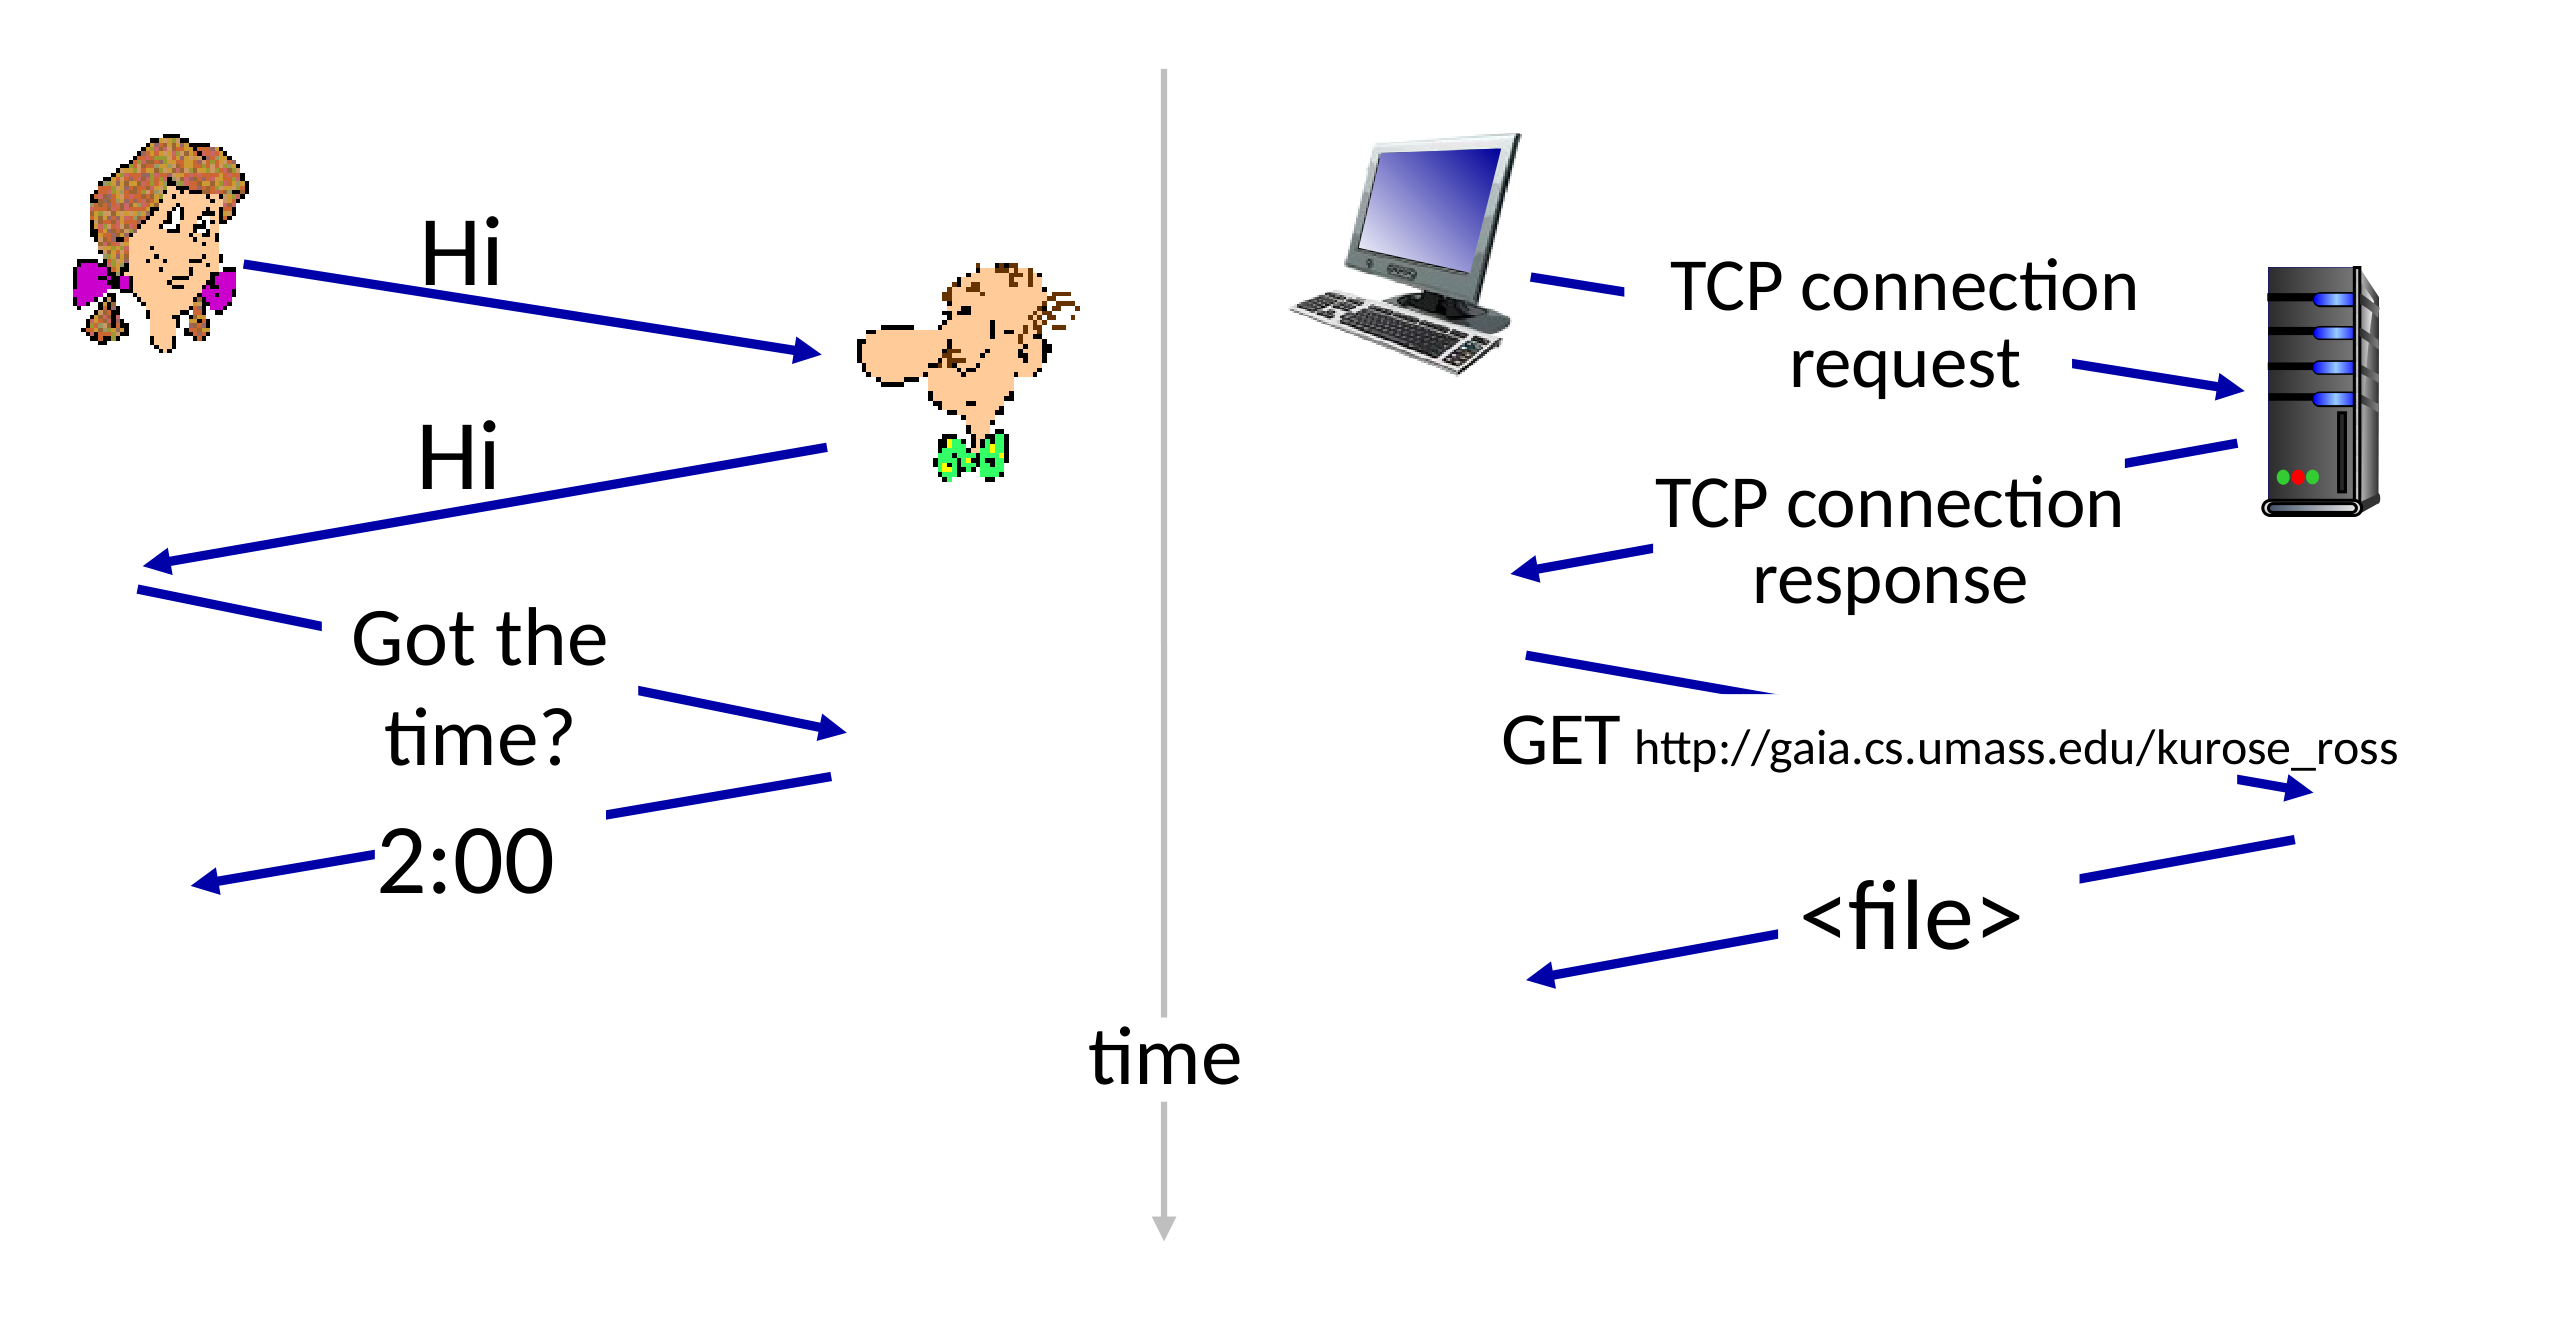
\includegraphics[width=0.62\linewidth]{cap02/protocollo_umano_rete.png}
    \caption{Stessa forma: un saluto, una risposta, poi la richiesta vera e propria.}
\end{figure}

\subsection{Chi scrive gli standard}

\begin{itemize}
    \item L'\textbf{IETF} (\emph{Internet Engineering Task Force}) è una comunità aperta di esperti che
          definisce gli standard e i protocolli di Internet.
    \item Lavora in \textbf{working group aperti}, ciascuno dedicato a un aspetto di Internet.
    \item Ogni gruppo pubblica documenti numerati detti \textbf{RFC} (\emph{Request For Comments}), che
          descrivono e definiscono protocolli, formati e metodi. Per esempio IPv4 è definito
          nell'\textbf{RFC 791}, del 1981. Il nome è rimasto per ragioni storiche: nascevano come inviti
          alla discussione e sono diventati gli standard di Internet.
    \item L'\textbf{ISO} (\emph{International Standards Organization}) funziona in modo molto diverso: è
          un'organizzazione non basata su trattati internazionali, i cui membri sono gli enti nazionali
          di standardizzazione. È da qui che nasce il modello \textbf{OSI}.
\end{itemize}

\info{Come decide Internet}{
    Gli standard di Internet non nascono da un voto in commissione, ma dal principio
    \emph{rough consensus and running code}: consenso di massima e codice che funziona. Una specifica
    che nessuno implementa non diventa uno standard.
}

% ══════════════════════════════════════════════════════════════
\section{La stratificazione}
% ══════════════════════════════════════════════════════════════

Le reti sono complesse e fatte di molti pezzi: host, router, collegamenti su mezzi diversi,
applicazioni, protocolli, hardware, software. C'è speranza di organizzarne la struttura? Sì:
la risposta architetturale è una \textbf{pila di strati}, ciascuno costruito su quello sottostante.

\dfn{Modello a strati}{
    Un approccio architetturale in cui la comunicazione è realizzata da una pila di \textbf{strati}
    (\emph{layer}) tali che:
    \begin{itemize}
      \item ogni strato è un \textbf{livello di astrazione}: nasconde \emph{come} svolge il proprio compito;
      \item ogni strato \textbf{usa i servizi dello strato inferiore} e \textbf{fornisce servizi allo
            strato superiore};
      \item tra due strati adiacenti c'è un'\textbf{interfaccia}: l'insieme delle operazioni che lo
            strato inferiore mette a disposizione di quello superiore.
    \end{itemize}
    La cima della pila è rivolta alle applicazioni (alto livello), il fondo all'hardware (basso livello).
}

\begin{figure}[H]
\centering
\begin{minipage}{0.33\linewidth}\centering
  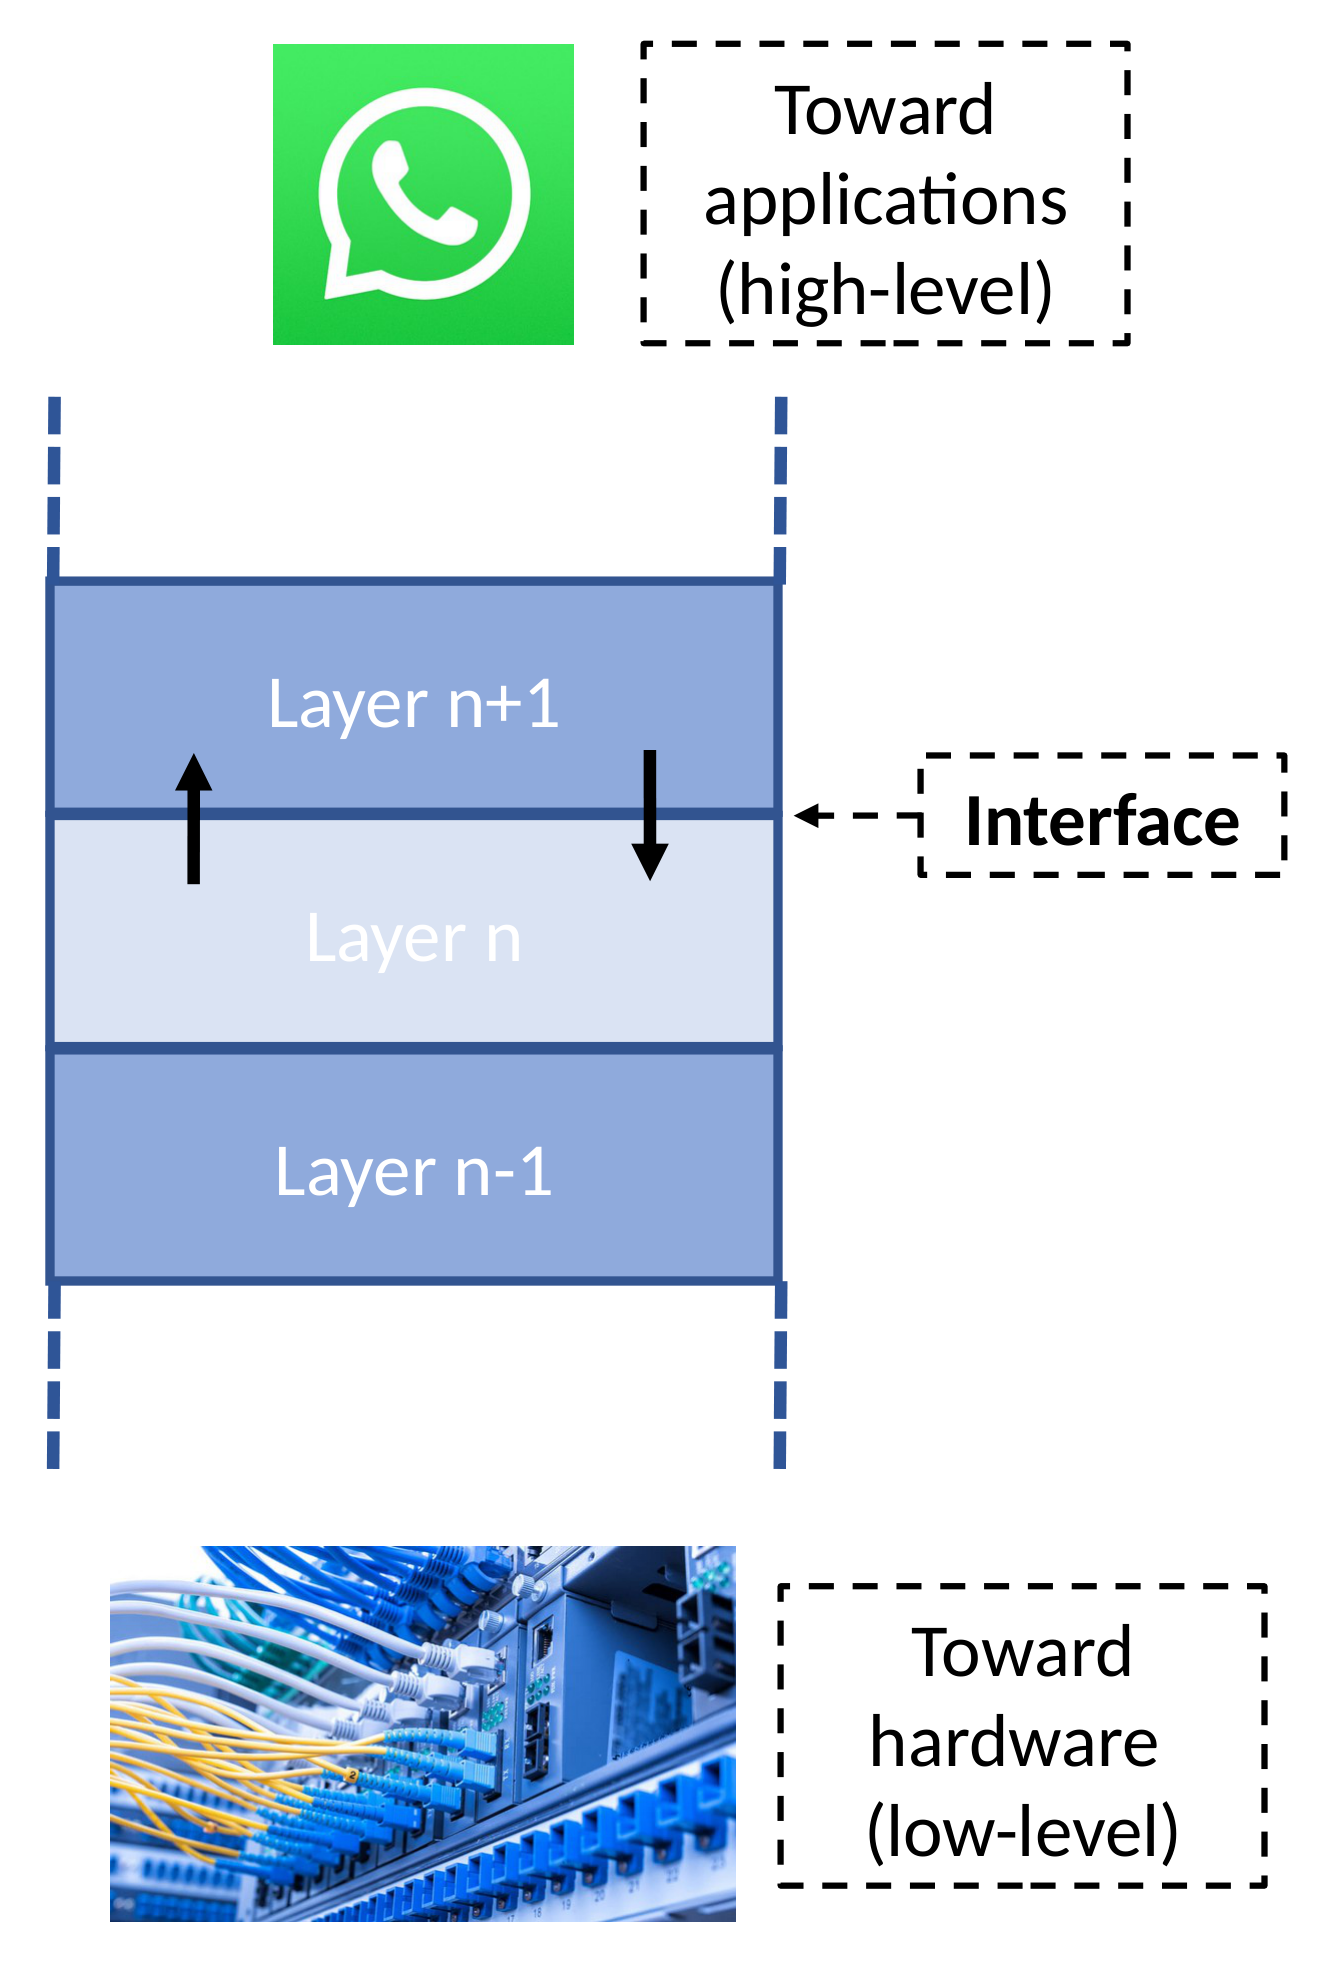
\includegraphics[width=0.85\linewidth]{cap02/stratificazione.png}
\end{minipage}
\begin{minipage}{0.55\linewidth}\centering
\begin{tikzpicture}[every node/.style={font=\small\sffamily}]
  \node[lay app, minimum width=3.4cm] (n1) at (0,1.4) {strato $n+1$};
  \node[lay tra, minimum width=3.4cm] (n) at (0,0) {strato $n$};
  \node[lay net, minimum width=3.4cm] (n0) at (0,-1.4) {strato $n-1$};
  \draw[{Stealth}-{Stealth}, thick] (n1) -- node[right, lbl] {interfaccia $n/n+1$} (n);
  \draw[{Stealth}-{Stealth}, thick] (n) -- node[right, lbl] {interfaccia $n-1/n$} (n0);
  \node[lbl, text width=3cm, align=left] at (-4,0.7) {lo strato $n$ \textbf{fornisce} servizi allo strato $n+1$\dots};
  \node[lbl, text width=3cm, align=left] at (-4,-0.7) {\dots\ \textbf{usando} i servizi dello strato $n-1$};
  \draw[-{Stealth}, primary, thick] (2.6,2) -- node[right, lbl] {verso le applicazioni} (2.6,2.6);
  \draw[-{Stealth}, primary, thick] (2.6,-2) -- node[right, lbl] {verso l'hardware} (2.6,-2.6);
\end{tikzpicture}
\end{minipage}
\caption{Ogni strato si appoggia a quello sotto e serve quello sopra, attraverso un'interfaccia.}
\end{figure}

\subsection{Moduli, interfacce e incapsulamento delle funzioni}

L'idea non è nuova: è la stessa che si usa per progettare qualunque software di una certa dimensione. Quando
un sistema viene diviso in sottosistemi, per ciascuno si stabilisce un'\textbf{interfaccia}, cioè l'insieme
dei servizi che il modulo offre all'esterno; \emph{come} quei servizi siano realizzati resta nascosto dentro
il modulo. È l'\textbf{incapsulamento delle funzioni}: ogni modulo può chiamare i servizi di un altro per il
proprio funzionamento, senza sapere nulla della sua implementazione. Chi ha scritto classi in C++ o in Java
ha già fatto esattamente questo: metodi pubblici all'esterno, dettagli privati all'interno.

\begin{figure}[H]
\centering
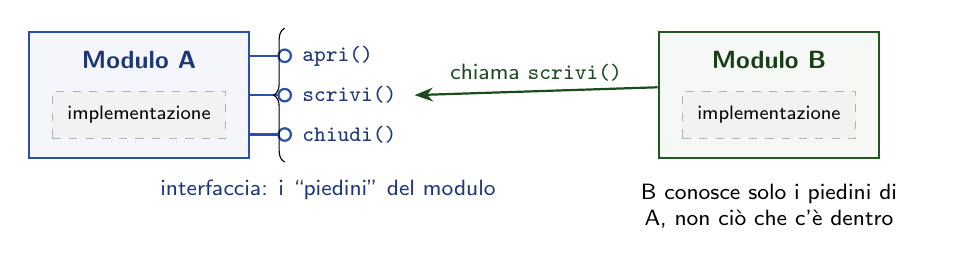
\begin{tikzpicture}[every node/.style={font=\footnotesize\sffamily}]
  % modulo A (offre servizi)
  \node[draw=netblue, thick, minimum width=2.8cm, minimum height=1.6cm, fill=netblue!5] (A) at (0,0) {};
  \node[text=netblue!70!black, font=\small\bfseries\sffamily] at (0,0.45) {Modulo A};
  \node[draw=black!30, dashed, fill=black!5, minimum width=2.2cm, minimum height=0.6cm, font=\scriptsize\sffamily] at (0,-0.25) {implementazione};
  \foreach \y/\n [count=\i] in {0.5/apri, 0/scrivi, -0.5/chiudi} {
    \draw[thick, netblue] (1.4,\y) -- (1.85,\y) node[pinint, draw=netblue] (pa\i) {};
    \node[anchor=west, text=netblue!70!black] at (1.95,\y) {\texttt{\n()}};
  }
  % modulo B (usa i servizi)
  \node[draw=netgreen!70!black, thick, minimum width=2.8cm, minimum height=1.6cm, fill=netgreen!5] (B) at (8,0) {};
  \node[text=netgreen!50!black, font=\small\bfseries\sffamily] at (8,0.45) {Modulo B};
  \node[draw=black!30, dashed, fill=black!5, minimum width=2.2cm, minimum height=0.6cm, font=\scriptsize\sffamily] at (8,-0.25) {implementazione};
  \draw[-{Stealth}, thick, netgreen!60!black] ([yshift=0.1cm]B.west) -- node[above, lbl] {chiama \texttt{scrivi()}} (3.5,0);
  \draw[decorate, decoration={brace, amplitude=4pt}] (1.85,-0.85) -- (1.85,0.85);
  \node[lbl, text=netblue!70!black, anchor=north] at (2.4,-0.95) {interfaccia: i ``piedini'' del modulo};
  \node[lbl, text width=4.2cm, anchor=north] at (8,-1.0) {B conosce solo i piedini di A, non ciò che c'è dentro};
\end{tikzpicture}
\caption{Ogni modulo espone all'esterno i propri servizi (i ``piedini'') e nasconde l'implementazione: è il disegno fatto alla lavagna per introdurre gli strati.}
\end{figure}

Nell'architettura a strati questa idea diventa più \textbf{rigida}: i moduli sono impilati, e ogni strato
offre i propri servizi allo strato \textbf{immediatamente superiore} e usa quelli dello strato
\textbf{immediatamente inferiore} per implementarli. Lo strato in cima è quello delle applicazioni (o offerto
alle applicazioni); quello più in basso è l'hardware, lo strato fisico.

\info{Architetture chiuse e aperte}{
    Nella concezione di base l'architettura a strati è \textbf{chiusa}: uno strato può rivolgersi soltanto a
    quello subito sotto. In alcuni casi, per efficienza o per necessità, la si \textbf{apre}, permettendo a uno
    strato di usare direttamente servizi di strati non adiacenti. È un'eccezione, e ha un prezzo: i moduli
    diventano meno indipendenti.
}

\subsection{La stratificazione non è un'idea delle reti}

Pile di strati le usate già, ovunque un sistema sia diventato troppo grande per essere progettato
in un pezzo solo.

\begin{figure}[H]
\centering
\begin{tikzpicture}[every node/.style={font=\small\sffamily}]
  \begin{scope}
    \node[font=\bfseries\sffamily] at (0,3.1) {Un sistema operativo};
    \node[layer, fill=lapp!60, minimum width=3.6cm] (a) at (0,2.2) {Applicazioni};
    \node[layer, fill=ltra!60, minimum width=3.6cm] (o) at (0,1.2) {Sistema operativo};
    \node[layer, fill=lnet!60, minimum width=3.6cm] (d) at (0,0.2) {Driver};
    \node[layer, fill=lphy, minimum width=3.6cm] (h) at (0,-0.8) {Hardware};
    \node[font=\ttfamily\small] (vim) at (3.2,2.9) {vim};
    \draw[-{Stealth}, netred, thick] (vim) to[out=-90, in=0] node[right, lbl, text=netred] {\texttt{write}} (a.east);
    \draw[-{Stealth}, netred, thick] ([xshift=1.2cm]a.south) -- ([xshift=1.2cm]o.north);
    \draw[-{Stealth}, netred, thick] ([xshift=1.2cm]o.south) -- ([xshift=1.2cm]d.north);
    \draw[-{Stealth}, netred, thick] ([xshift=1.2cm]d.south) -- ([xshift=1.2cm]h.north);
    \node[lbl, text width=4cm] at (0,-1.7) {una sola \texttt{write} attraversa quattro interfacce};
  \end{scope}
  \begin{scope}[xshift=8.5cm]
    \node[font=\bfseries\sffamily] at (0,3.1) {Un sistema informativo};
    \node[layer, fill=lapp!60, minimum width=3.6cm] (ui) at (0,2.2) {Interfaccia utente};
    \node[layer, fill=ltra!60, minimum width=3.6cm] (la) at (0,1.2) {Logica applicativa};
    \node[layer, fill=lnet!60, minimum width=3.6cm] (gd) at (0,0.2) {Gestione dei dati};
    \node[cylinder, shape border rotate=90, aspect=0.25, draw, fill=lphy, minimum height=0.9cm, minimum width=0.8cm] (db) at (2.8,0.2) {DB};
    \draw[thick] (gd) -- (db);
    \node at (-2.8,2.8) {\icon[0.7cm]{laptop}};
    \draw[thick, -{Stealth}] (-2.6,2.5) -- (ui.west);
    \node[lbl, text width=4.4cm] at (0,-0.9) {architettura a tre strati: l'utente non tocca mai direttamente il database};
  \end{scope}
\end{tikzpicture}
\caption{Due pile di strati che conoscete già.}
\end{figure}

Le reti sono semplicemente il caso più grande di tutti.

\subsection{Cosa guadagniamo, e cosa paghiamo}

\begin{itemize}
    \item \textbf{Struttura}: una struttura esplicita permette di \textbf{dare un nome} ai pezzi del
          sistema e alle loro relazioni; è un \emph{modello di riferimento} di cui discutere.
    \item \textbf{Modularità}: l'implementazione di uno strato può cambiare senza che nient'altro si
          muova, \textbf{purché il servizio offerto resti lo stesso}. Sostituire tutte le linee
          telefoniche con canali satellitari è una modifica interna a un solo strato: gli strati
          superiori non se ne accorgono.
\end{itemize}

\begin{esempio}{La modularità nella vita di tutti i giorni}
\begin{itemize}
    \item Cambiate stampante, e con lei il \textbf{driver}: il sistema operativo continua a mandare le stampe
          esattamente come prima, e le applicazioni non si accorgono di nulla.
    \item State scrivendo un messaggio collegati al Wi-Fi di casa, poi uscite e il telefono passa alla
          \textbf{rete cellulare}. L'applicazione di messaggistica si rivolge sempre al sistema operativo nello
          stesso modo: del cambio di tecnologia si occupano gli strati inferiori.
\end{itemize}
\end{esempio}

\info{L'analogia del viaggio aereo}{
    Un viaggio in aereo è una pila di servizi: biglietto (acquisto / reclamo), bagagli (imbarco /
    ritiro), gate (imbarco / sbarco), pista (decollo / atterraggio), rotta dell'aereo. Ogni ``strato''
    dell'aeroporto di partenza ha il suo corrispondente in quello di arrivo, e se cambia la procedura
    ai gate il resto del sistema non se ne accorge.
}

\warning{Il prezzo dell'architettura a strati}{
    La domanda ``\emph{layering considered harmful?}'' non è retorica. Alla lavagna il prezzo è stato riassunto
    in tre voci:
    \begin{itemize}
      \item \textbf{maggiore complessità}: tutte le \textbf{interfacce} tra gli strati vanno progettate e
            implementate, e ogni strato aggiunge le proprie informazioni di controllo (\textbf{overhead});
      \item \textbf{eventuali ridondanze}: uno strato può rifare qualcosa che uno strato inferiore fa già, per
            esempio la rilevazione e la correzione degli errori, svolta sia su ogni singolo collegamento sia da
            un estremo all'altro. Più calcolo, a volte inutile;
      \item \textbf{rigidità}: le informazioni interne di ogni strato sono \textbf{nascoste}. Quando poi uno
            strato ha bisogno di un'informazione che sta in un altro (succede spesso nelle reti), le strade sono
            due: \textbf{riprogettare} gli strati, oppure adottare soluzioni ``\emph{quick and dirty}'', rapide,
            efficaci e un po' sporche, come vedremo per esempio con l'uso delle porte.
    \end{itemize}
    È un compromesso: si accetta un po' di inefficienza in cambio di un'enorme semplicità di progetto.
}

% ══════════════════════════════════════════════════════════════
\section{Servizio, interfaccia e protocollo}
% ══════════════════════════════════════════════════════════════

Tre concetti da tenere rigorosamente separati.

\dfn{Servizio e protocollo}{
    Un \textbf{servizio} è l'insieme delle operazioni che uno strato offre allo strato superiore: dice
    \textbf{che cosa} fa lo strato, mai \textbf{come} lo fa.

    Un \textbf{protocollo} è l'insieme delle regole sul formato e sul significato dei messaggi
    scambiati con l'\textbf{entità paritaria} (\emph{peer entity}), cioè lo stesso strato sull'altra
    macchina.
}

\begin{figure}[H]
    \centering
    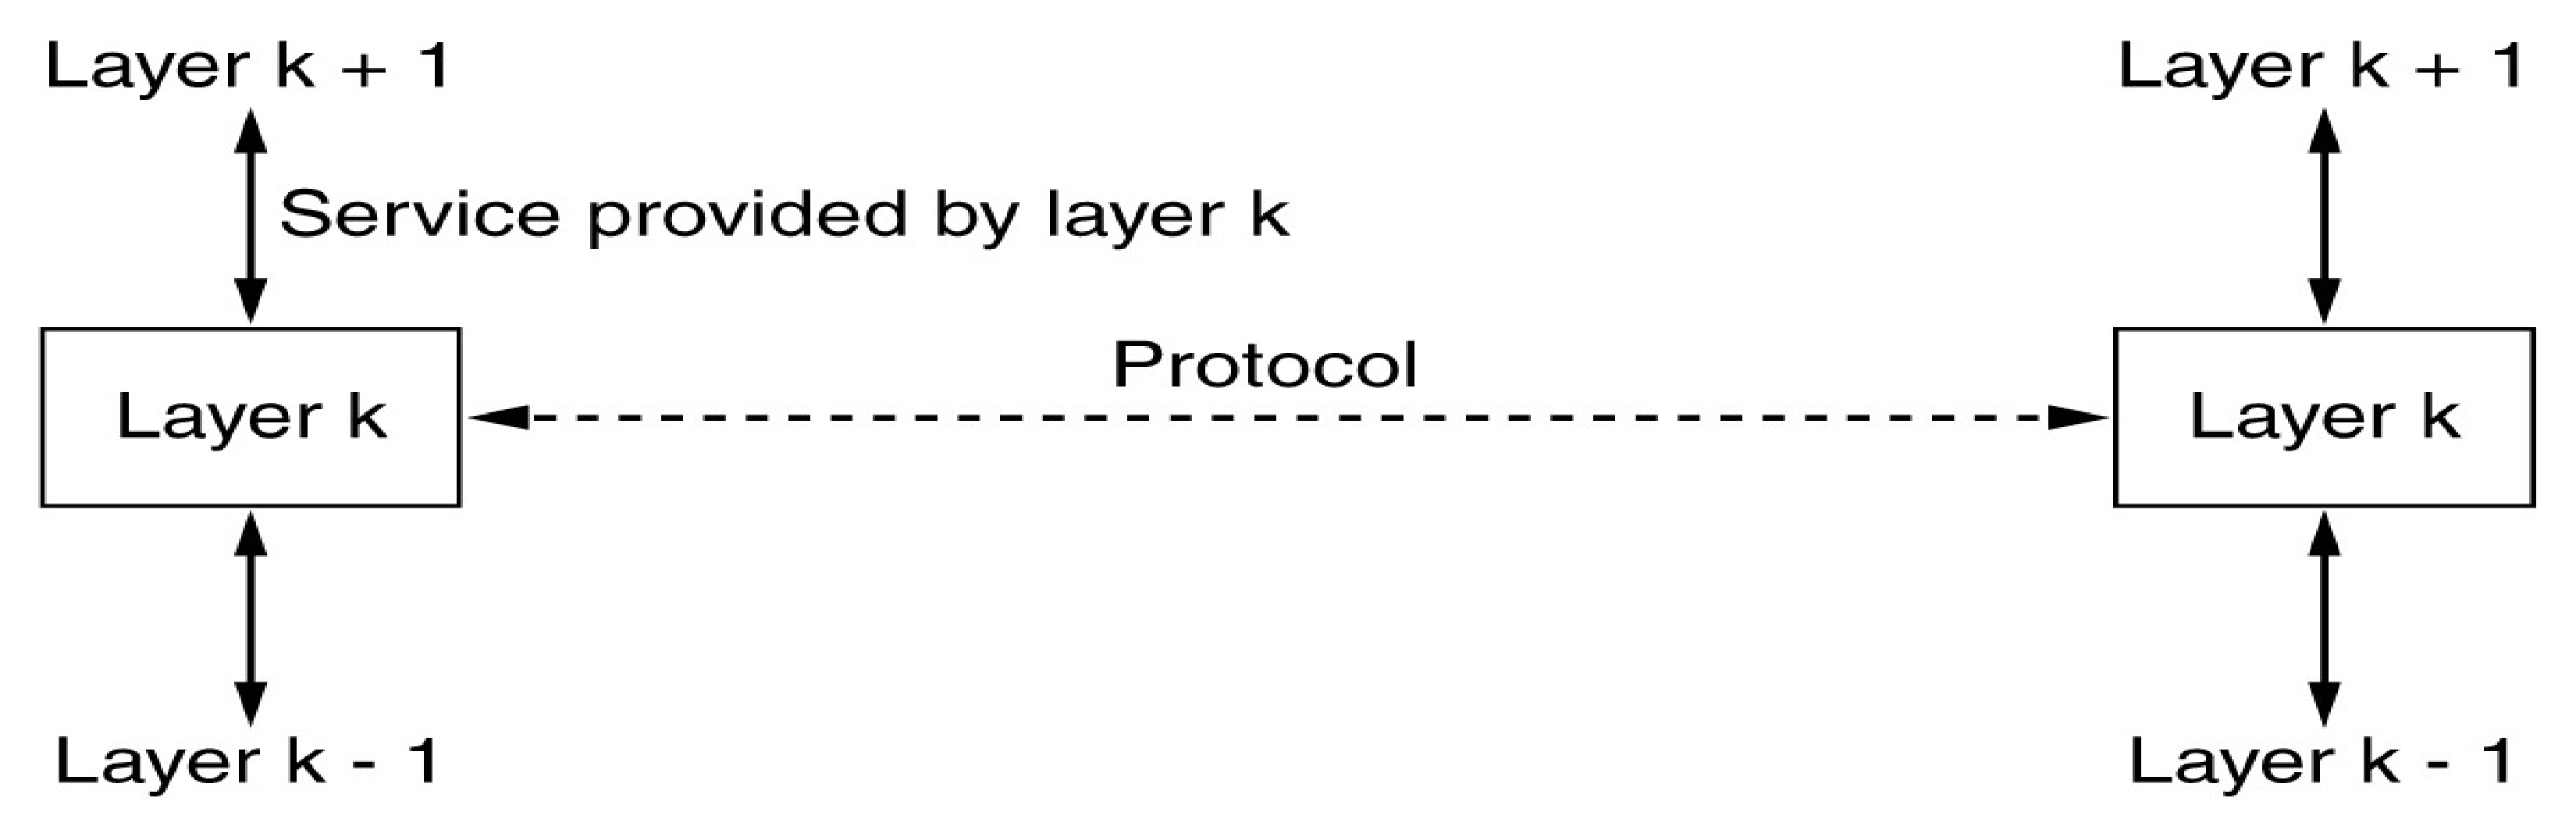
\includegraphics[width=0.62\linewidth]{cap02/servizio_protocollo.png}
    \caption{I servizi stanno sulle interfacce verticali, i protocolli sullo scambio orizzontale.}
\end{figure}

L'\textbf{interfaccia} è il punto in cui il servizio viene offerto: l'insieme delle operazioni che
lo strato inferiore rende disponibili a quello superiore. In sintesi:

\begin{center}
\begin{tabular}{lll}
\toprule
\textbf{Concetto} & \textbf{Direzione} & \textbf{Risponde alla domanda} \\
\midrule
Servizio & verticale (tra strati adiacenti) & \emph{che cosa} offre lo strato? \\
Interfaccia & verticale & \emph{come si chiede} il servizio? \\
Protocollo & orizzontale (tra strati omologhi) & \emph{come} lo strato realizza il servizio? \\
\bottomrule
\end{tabular}
\end{center}

\dfn{Entità e protocolli}{
    Le \textbf{entità} (gli elementi attivi di uno strato, hardware o software) \textbf{usano i
    protocolli per implementare i servizi} che offrono.
}

\warning{Servizio e protocollo sono indipendenti}{
    Uno strato può cambiare completamente protocollo senza che gli strati superiori se ne accorgano,
    purché il servizio offerto resti lo stesso. Confondere servizio e protocollo è un errore tipico.
}

\begin{esempio}{Un messaggio alla zia}
Premete ``invia'' sulla vostra applicazione di messaggistica. L'applicazione non trasmette nulla da sé: chiama
il servizio di invio che il \textbf{livello di trasporto} del telefono offre attraverso la propria interfaccia,
e da quel momento se ne disinteressa. Il livello di trasporto dialoga, con il \textbf{protocollo di trasporto},
con l'entità di trasporto sul telefono della zia; per farlo usa i servizi del \textbf{livello di rete}, che a
sua volta dialoga con il livello di rete dall'altra parte, occupandosi di attraversare la topologia di Internet.
\begin{center}
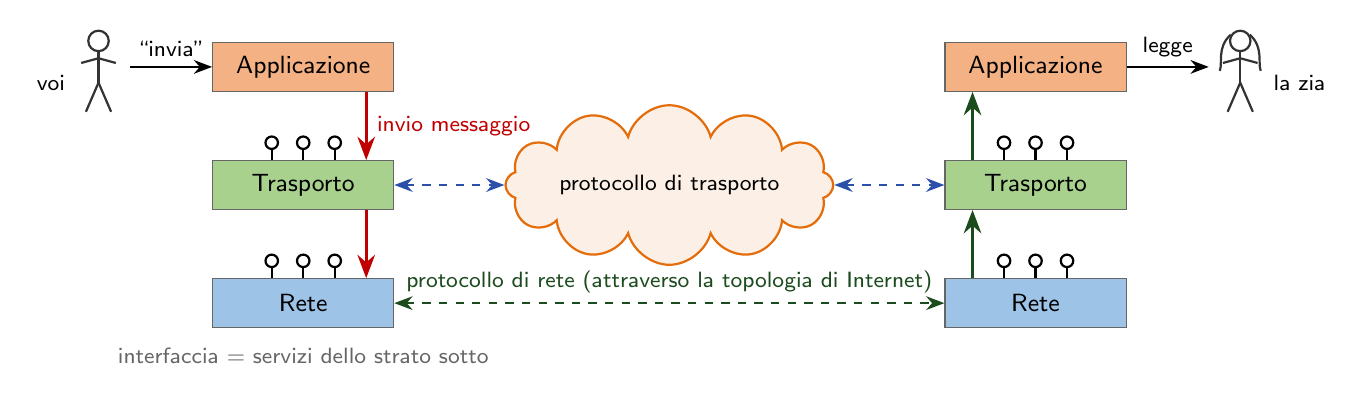
\begin{tikzpicture}[every node/.style={font=\footnotesize\sffamily}]
  % mittente
  \pic[black!80] at (-2.6,1.55) {persona};
  \node[anchor=east] at (-2.9,1.6) {voi};
  \node[lay app, minimum width=2.3cm] (a1) at (0,1.8) {Applicazione};
  \node[lay tra, minimum width=2.3cm] (t1) at (0,0.3) {Trasporto};
  \node[lay net, minimum width=2.3cm] (n1) at (0,-1.2) {Rete};
  \draw[-{Stealth}, thick] (-2.2,1.8) -- node[above, lbl] {``invia''} (a1.west);
  % destinataria
  \pic[black!80] at (11.9,1.55) {personacapelli};
  \node[anchor=west] at (12.2,1.6) {la zia};
  \node[lay app, minimum width=2.3cm] (a2) at (9.3,1.8) {Applicazione};
  \node[lay tra, minimum width=2.3cm] (t2) at (9.3,0.3) {Trasporto};
  \node[lay net, minimum width=2.3cm] (n2) at (9.3,-1.2) {Rete};
  \draw[-{Stealth}, thick] (a2.east) -- node[above, lbl] {legge} (11.5,1.8);
  % piedini delle interfacce
  \foreach \st in {t1,n1,t2,n2} \foreach \dx in {-0.4,0,0.4} \draw[thick] ([xshift=\dx cm]\st.north) -- ++(0,0.22) node[pinint] {};
  \draw[-{Stealth}, very thick, netred] ([xshift=0.8cm]a1.south) -- node[right, lbl, text=netred] {invio messaggio} ([xshift=0.8cm]t1.north);
  \draw[-{Stealth}, very thick, netred] ([xshift=0.8cm]t1.south) -- ([xshift=0.8cm]n1.north);
  \draw[-{Stealth}, very thick, netgreen!60!black] ([xshift=-0.8cm]n2.north) -- ([xshift=-0.8cm]t2.south);
  \draw[-{Stealth}, very thick, netgreen!60!black] ([xshift=-0.8cm]t2.north) -- ([xshift=-0.8cm]a2.south);
  % protocolli
  \node[cloud, cloud puffs=12, aspect=3.2, draw=netorange, fill=netorange!10, thick, minimum width=2.6cm, minimum height=0.8cm, inner sep=1pt] (pr) at (4.65,0.3) {protocollo di trasporto};
  \draw[{Stealth}-{Stealth}, dashed, thick, netblue] (t1.east) -- (pr.west);
  \draw[{Stealth}-{Stealth}, dashed, thick, netblue] (pr.east) -- (t2.west);
  \draw[{Stealth}-{Stealth}, dashed, thick, netgreen!60!black] (n1.east) -- node[above, lbl] {protocollo di rete (attraverso la topologia di Internet)} (n2.west);
  \node[lbl, text=black!60, anchor=north] at (0,-1.65) {interfaccia = servizi dello strato sotto};
\end{tikzpicture}
\end{center}
Tra uno strato e quello sotto, \textbf{nello stesso telefono}, c'è un'\textbf{interfaccia} (i piedini); tra due
entità dello stesso strato, \textbf{su telefoni diversi}, c'è un \textbf{protocollo} (le frecce tratteggiate).
\end{esempio}

\subsection{Strati omologhi: comunicazione virtuale e fisica}

\begin{figure}[H]
    \centering
    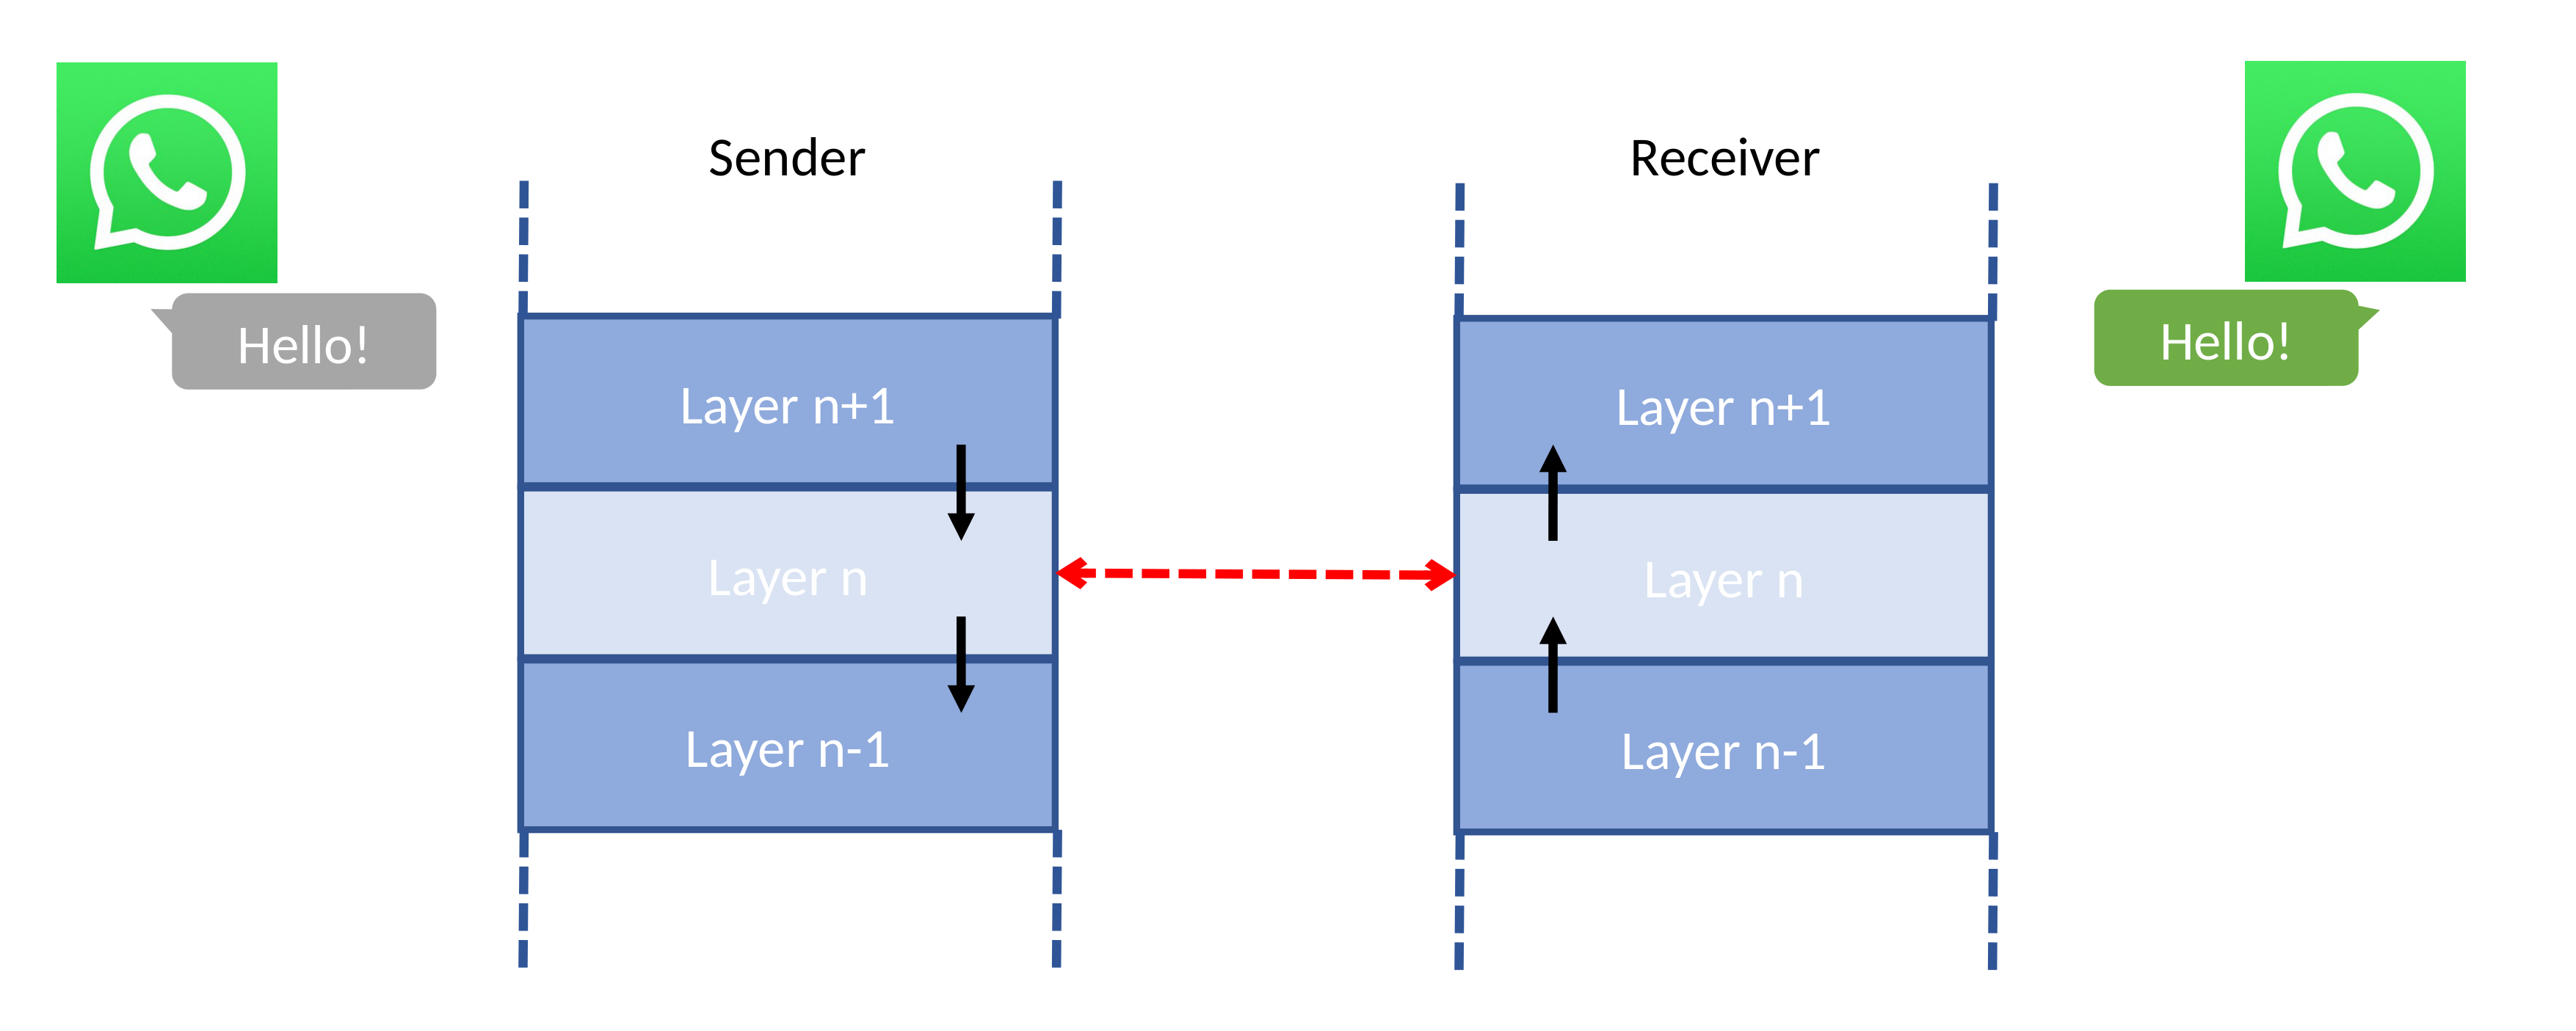
\includegraphics[width=0.62\linewidth]{cap02/strati_omologhi.png}
    \caption{Lo strato $n$ del mittente dialoga logicamente con lo strato $n$ del destinatario.}
\end{figure}

\dfn{Comunicazione orizzontale}{
    Quando due dispositivi comunicano, \textbf{ogni strato del mittente comunica con lo stesso strato
    del destinatario}, e con nient'altro, per mezzo di uno specifico protocollo.
}

\begin{itemize}
    \item Quella freccia orizzontale \textbf{non è un cavo}: è una conversazione \emph{logica}.
    \item I dati \textbf{scendono} realmente lungo la pila del mittente e \textbf{risalgono} quella del
          destinatario. Solo al livello fisico qualcosa viaggia davvero.
    \item La catena si ripete a ogni strato: per fornire i propri servizi uno strato deve comunicare con il suo
          pari, e per farlo chiama i servizi dello strato inferiore, che a sua volta comunica con il proprio pari
          usando un protocollo \textbf{diverso}, e così via fino al protocollo fisico, che manda segnali su un mezzo.
\end{itemize}

\warning{Tutte queste trasmissioni sono virtuali}{
    Nelle reti c'è comunicazione tra due macchine a \textbf{ogni} strato, con i relativi protocolli. Ma
    tutte queste trasmissioni sono \textbf{virtuali}, salvo quella a livello fisico, che è l'unica a
    comportare effettivi fenomeni fisici. Il livello di trasporto del mittente ``crede'' di parlare
    direttamente con il trasporto del destinatario, ma i suoi dati scendono lungo tutta la pila,
    viaggiano sul filo e risalgono dall'altra parte.
}

\begin{esempio}{L'analogia postale}
Il modello a strati funziona come il servizio postale: ogni strato fa un solo lavoro, si affida allo strato
sotto e parla il proprio ``linguaggio''; ogni indirizzo è letto dallo strato per cui è stato scritto, e da
nessun altro.
\begin{center}
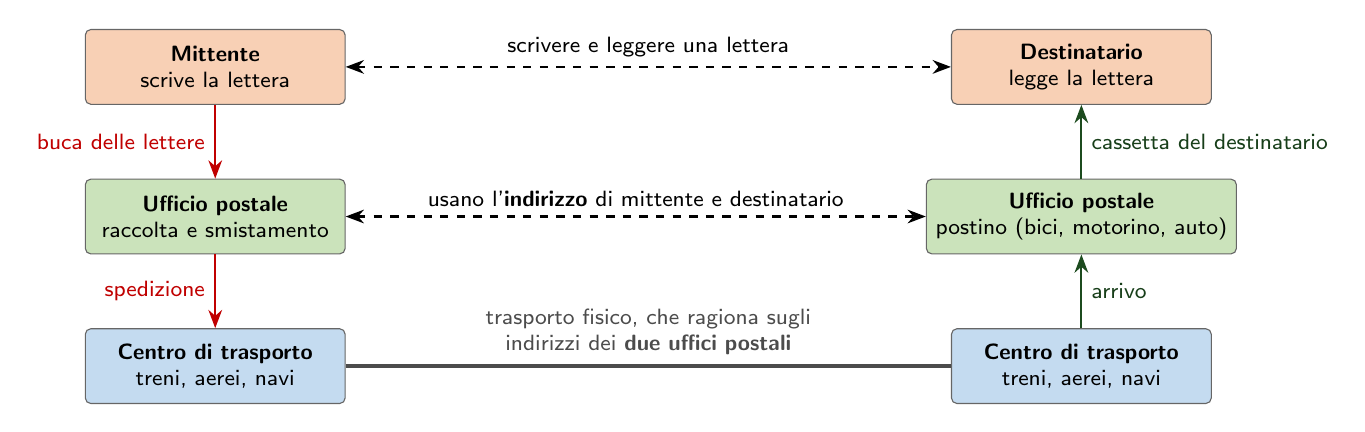
\begin{tikzpicture}[every node/.style={font=\footnotesize\sffamily},
    pbox/.style={draw=black!60, rounded corners=2pt, minimum width=3.3cm, minimum height=0.95cm, align=center}]
  % colonna sinistra
  \node[pbox, fill=lapp!60] (m) at (0,0) {\textbf{Mittente}\\scrive la lettera};
  \node[pbox, fill=ltra!60] (u1) at (0,-1.9) {\textbf{Ufficio postale}\\raccolta e smistamento};
  \node[pbox, fill=lnet!60] (x1) at (0,-3.8) {\textbf{Centro di trasporto}\\treni, aerei, navi};
  % colonna destra
  \node[pbox, fill=lapp!60] (d) at (11,0) {\textbf{Destinatario}\\legge la lettera};
  \node[pbox, fill=ltra!60] (u2) at (11,-1.9) {\textbf{Ufficio postale}\\postino (bici, motorino, auto)};
  \node[pbox, fill=lnet!60] (x2) at (11,-3.8) {\textbf{Centro di trasporto}\\treni, aerei, navi};
  % interfacce verticali
  \draw[-{Stealth}, thick, netred] (m) -- node[left, lbl, text=netred] {buca delle lettere} (u1);
  \draw[-{Stealth}, thick, netred] (u1) -- node[left, lbl, text=netred] {spedizione} (x1);
  \draw[-{Stealth}, thick, netgreen!60!black] (x2) -- node[right, lbl, text=netgreen!50!black] {arrivo} (u2);
  \draw[-{Stealth}, thick, netgreen!60!black] (u2) -- node[right, lbl, text=netgreen!50!black] {cassetta del destinatario} (d);
  % dialoghi orizzontali
  \draw[{Stealth}-{Stealth}, dashed, thick] (m) -- node[above, lbl] {scrivere e leggere una lettera} (d);
  \draw[{Stealth}-{Stealth}, dashed, thick] (u1) -- node[above, lbl] {usano l'\textbf{indirizzo} di mittente e destinatario} (u2);
  \draw[very thick, black!70] (x1) -- node[above, lbl, text width=6.5cm] {trasporto fisico, che ragiona sugli indirizzi dei \textbf{due uffici postali}} (x2);
\end{tikzpicture}
\end{center}
\begin{itemize}
    \item \textbf{Strato superiore}: mittente e destinatario vedono soltanto due buche per le lettere, una in cui
          infilare la lettera e una da cui ritirarla. I loro ``protocolli'' sono scrivere e leggere una lettera.
    \item \textbf{Strato intermedio}: gli uffici postali raccolgono la lettera e, dall'altra parte, la fanno
          consegnare dal postino. Il loro linguaggio sono gli \textbf{indirizzi} del mittente e del destinatario.
    \item \textbf{Strato inferiore}: treni, aerei e navi portano fisicamente la posta da un ufficio all'altro, e
          ragionano solo in termini di uffici di provenienza e di destinazione.
\end{itemize}
Tanenbaum propone un'analogia altrettanto efficace: un filosofo che detta una lettera a un traduttore, il
quale la passa a una segretaria che la spedisce; dall'altra parte la catena si ripercorre al contrario, e ogni
figura ``parla'' solo con la figura corrispondente.
\end{esempio}

% ══════════════════════════════════════════════════════════════
\section{Servizi con e senza connessione}
% ══════════════════════════════════════════════════════════════

Prima di vedere gli strati concreti, serve una distinzione \textbf{ortogonale} a quella degli strati:
quella tra servizi \textbf{orientati alla connessione} e servizi \textbf{senza connessione}.

\subsection{Servizio orientato alla connessione}

\dfn{Servizio orientato alla connessione}{
    Modellato sul \textbf{sistema telefonico}: l'utente del servizio prima \textbf{stabilisce} una
    connessione, poi la \textbf{usa}, infine la \textbf{rilascia}.
}

\begin{itemize}
    \item La connessione si comporta come un \textbf{tubo}: ciò che entra da un'estremità esce
          dall'altra, normalmente \textbf{nello stesso ordine}.
    \item L'apertura permette una \textbf{negoziazione} dei parametri (dimensione massima dei messaggi,
          qualità del servizio, \dots): una parte propone, l'altra accetta o fa una controproposta.
    \item Una connessione che riserva anche delle \textbf{risorse}, per esempio una velocità fissa, si
          chiama \textbf{circuito}: un cammino sulla rete su cui viaggiano tutti i dati della sessione.
    \item Conviene quando c'è una quantità significativa di dati da scambiare.
\end{itemize}

E se si ha un solo messaggio breve da inviare, vale la pena aprire e chiudere una connessione?

\subsection{Servizio senza connessione}

\dfn{Servizio senza connessione (connectionless)}{
    Modellato sul \textbf{sistema postale}: non si stabilisce nulla prima di trasmettere. Ogni
    messaggio porta con sé l'\textbf{indirizzo completo} di destinazione e viene \textbf{gestito
    individualmente} dai nodi intermedi.
}

\begin{figure}[H]
\centering
\begin{tikzpicture}[every node/.style={font=\footnotesize\sffamily}]
  \node (A) at (0,0) {\icon[0.9cm]{pc}}; \node[below=-2pt of A] {A};
  \node (B) at (10,0) {\icon[1cm]{laptop}}; \node[below=-2pt of B] {B};
  \node[cloud, cloud puffs=14, aspect=2.6, draw=netblue!50, fill=cloudbg, minimum width=6.2cm, minimum height=3cm] at (5,0) {};
  \node[gnode] (n1) at (3,0.5) {}; \node[gnode] (n2) at (4.5,1) {}; \node[gnode] (n3) at (4.3,-0.8) {};
  \node[gnode] (n4) at (6,0.1) {}; \node[gnode] (n5) at (7,0.9) {}; \node[gnode] (n6) at (6.9,-0.8) {};
  \foreach \a/\b in {n1/n2, n1/n3, n2/n4, n3/n4, n2/n5, n4/n5, n4/n6, n3/n6, n5/n6} \draw[black!40, thick] (\a) -- (\b);
  \draw[wired] (A) -- (n1); \draw[wired] (n5) -- (B); \draw[wired] (n6) -- (B);
  \draw[netred, very thick, -{Stealth}] (n1) -- (n2) -- (n5);
  \draw[netgreen, very thick, -{Stealth}] (n1) -- (n3) -- (n6);
  \node[text=netred] at (3.4,1.55) {pacchetto 1};
  \node[text=netgreen] at (5.3,-1.45) {pacchetto 2};
  \fill[netred] (1.2,0.35) rectangle (1.6,0.6); \fill[netgreen] (1.8,0.35) rectangle (2.2,0.6);
  \node at (5,-2.1) {ogni pacchetto è gestito individualmente: può seguire un cammino diverso e arrivare fuori ordine};
\end{tikzpicture}
\caption{In un servizio senza connessione i pacchetti tra gli stessi due estremi possono seguire strade diverse.}
\end{figure}

\begin{itemize}
    \item Tra gli stessi due estremi la rete offre più cammini, quindi due messaggi possono seguirne
          di diversi e \textbf{arrivare fuori ordine}.
    \item Nella commutazione \textbf{store-and-forward} un nodo riceve un messaggio \textbf{per intero}
          prima di inoltrarlo al nodo successivo.
    \item Nella commutazione \textbf{cut-through} un nodo comincia a inoltrare il messaggio \textbf{prima}
          di averlo ricevuto completamente (appena ha letto l'indirizzo di destinazione).
\end{itemize}

\begin{figure}[H]
\centering
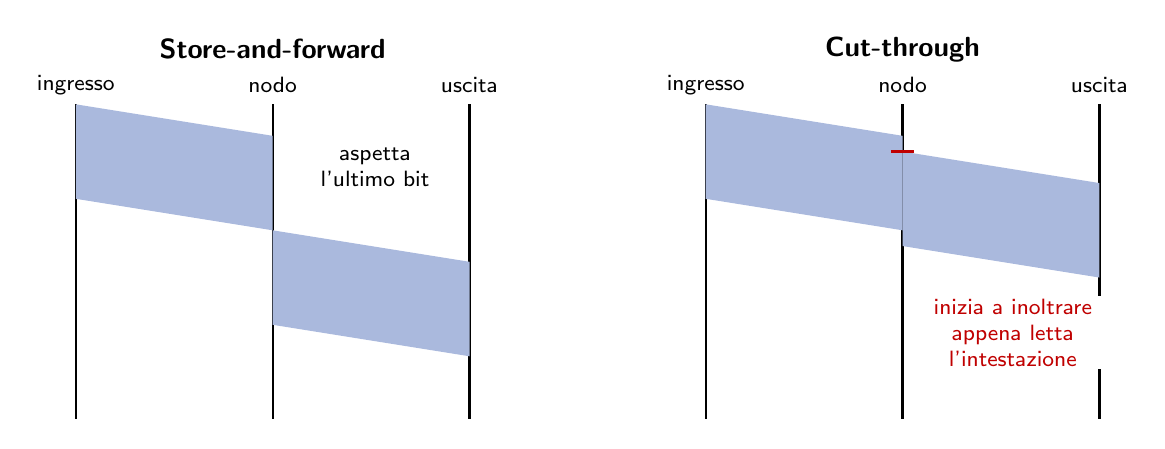
\begin{tikzpicture}[every node/.style={font=\footnotesize\sffamily}]
  \begin{scope}
    \node[font=\bfseries\sffamily] at (2.5,0.7) {Store-and-forward};
    \foreach \x/\n in {0/in, 2.5/nodo, 5/out} { \draw[thick] (\x,0) -- (\x,-4); }
    \node at (0,0.25) {ingresso}; \node at (2.5,0.25) {nodo}; \node at (5,0.25) {uscita};
    \fill[netblue!40] (0,0) -- (2.5,-0.4) -- (2.5,-1.6) -- (0,-1.2) -- cycle;
    \fill[netblue!40] (2.5,-1.6) -- (5,-2.0) -- (5,-3.2) -- (2.5,-2.8) -- cycle;
    \node[lbl, text width=2cm, fill=white, inner sep=1pt] at (3.8,-0.8) {aspetta l'ultimo bit};
  \end{scope}
  \begin{scope}[xshift=8cm]
    \node[font=\bfseries\sffamily] at (2.5,0.7) {Cut-through};
    \foreach \x in {0,2.5,5} { \draw[thick] (\x,0) -- (\x,-4); }
    \node at (0,0.25) {ingresso}; \node at (2.5,0.25) {nodo}; \node at (5,0.25) {uscita};
    \fill[netblue!40] (0,0) -- (2.5,-0.4) -- (2.5,-1.6) -- (0,-1.2) -- cycle;
    \fill[netblue!40] (2.5,-0.6) -- (5,-1.0) -- (5,-2.2) -- (2.5,-1.8) -- cycle;
    \draw[netred, thick] (2.35,-0.6) -- (2.65,-0.6);
    \node[lbl, text width=2.3cm, fill=white, inner sep=1pt, text=netred] at (3.9,-2.9) {inizia a inoltrare appena letta l'intestazione};
  \end{scope}
\end{tikzpicture}
\caption{Store-and-forward contro cut-through: il secondo riduce il ritardo, ma può inoltrare anche messaggi che si riveleranno danneggiati.}
\end{figure}

\dfn{Datagram}{
    Un servizio \textbf{senza connessione e inaffidabile}, cioè senza conferma di ricezione
    (\emph{unacknowledged}). Il nome richiama il \emph{telegramma}, che anch'esso non prevedeva
    ricevuta di ritorno.
}

\subsection{Affidabilità}

\dfn{Affidabilità}{
    Un servizio è \textbf{affidabile} se il ricevente \textbf{conferma} (\emph{acknowledgement}, ACK)
    ciò che ha ricevuto, così che il mittente sappia che è arrivato. L'affidabilità è
    \textbf{ortogonale} alla connessione: sia i servizi con connessione sia quelli senza possono essere
    affidabili o no.
}

Perché mai si dovrebbe rinunciare all'affidabilità?

\begin{itemize}
    \item Le conferme costano \textbf{overhead e ritardo}, e a volte il prezzo è troppo alto.
    \item L'affidabilità può semplicemente \textbf{non essere disponibile}: Ethernet non la fornisce, e
          sono gli strati superiori a dover recuperare gli errori.
    \item Nel \textbf{Voice over IP} confermare ogni pacchetto e ripristinarne l'ordine sarebbe non solo inutile ma
          dannoso: un ritardo di tre o quattro secondi rende una telefonata inutilizzabile, mentre una breve
          interruzione dell'audio si rimedia ripetendo una frase. Tutte le applicazioni VoIP cercano di
          \textbf{ridurre il ritardo} e accettano i buchi: l'inaffidabilità è la scelta \emph{giusta}, non un
          compromesso. I parametri della comunicazione vanno adattati alle esigenze dell'applicazione.
\end{itemize}

\info{Affidabile sopra inaffidabile}{
    La maggior parte dei servizi affidabili che vedremo nel corso è costruita \textbf{sopra} un servizio
    inaffidabile: TCP (affidabile) sopra IP (inaffidabile) ne è l'esempio principale.
}

\subsection{Sei tipi di servizio}

\begin{table}[H]
\centering
\begin{tabular}{lll}
\toprule
\textbf{Tipo} & \textbf{Servizio} & \textbf{Esempio} \\
\midrule
\multirow{3}{*}{Orientato alla connessione}
  & Flusso di messaggi affidabile & Sequenza di pagine \\
  & Flusso di byte affidabile & Download di un film \\
  & Connessione inaffidabile & Voice over IP \\
\midrule
\multirow{3}{*}{Senza connessione}
  & Datagram inaffidabile & Posta elettronica ``spazzatura'' \\
  & Datagram con conferma & Messaggi con le ``spunte'' di consegna \\
  & Richiesta-risposta (\emph{request-reply}) & Interrogazione a un database \\
\bottomrule
\end{tabular}
\caption{Sei servizi comuni, con e senza connessione.}
\end{table}

\info{Le due righe da ricordare}{
    Il \textbf{flusso di byte affidabile} è il servizio che ci darà \textbf{TCP}; il \textbf{datagram
    inaffidabile} è quello che ci darà \textbf{UDP}.
}

\subsection{Le primitive di servizio}

Un servizio si specifica formalmente tramite le \textbf{primitive}, cioè le operazioni con cui un
processo lo richiede. Quando la pila protocollare è implementata nel sistema operativo, le primitive
sono \textbf{chiamate di sistema} (\emph{system call}).

\begin{table}[H]
\centering
\begin{tabular}{ll}
\toprule
\textbf{Primitiva} & \textbf{Significato} \\
\midrule
\texttt{LISTEN} & si blocca in attesa di una connessione in ingresso \\
\texttt{CONNECT} & stabilisce una connessione con un peer in attesa \\
\texttt{ACCEPT} & accetta una connessione in ingresso da un peer \\
\texttt{RECEIVE} & si blocca in attesa di un messaggio in ingresso \\
\texttt{SEND} & invia un messaggio al peer \\
\texttt{DISCONNECT} & termina la connessione \\
\bottomrule
\end{tabular}
\caption{Le primitive di un semplice servizio orientato alla connessione.}
\end{table}

\begin{figure}[H]
\centering
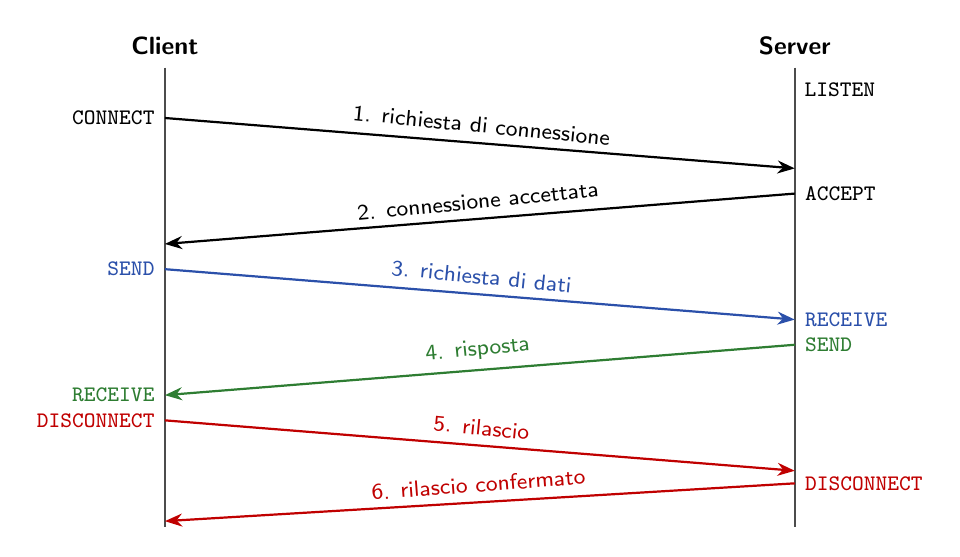
\begin{tikzpicture}[yscale=0.8, every node/.style={font=\footnotesize\sffamily}]
  \timeline{c}{0}{Client}{7.3}
  \timeline{s}{8}{Server}{7.3}
  \node[right, font=\ttfamily\footnotesize] at (8,-0.35) {LISTEN};
  \draw[msg] (0,-0.8) node[left, font=\ttfamily\footnotesize] {CONNECT} -- node[above, sloped] {1. richiesta di connessione} (8,-1.6);
  \draw[msg] (8,-2.0) node[right, font=\ttfamily\footnotesize] {ACCEPT} -- node[above, sloped] {2. connessione accettata} (0,-2.8);
  \draw[msg, netblue] (0,-3.2) node[left, font=\ttfamily\footnotesize] {SEND} -- node[above, sloped] {3. richiesta di dati} (8,-4.0) node[right, font=\ttfamily\footnotesize] {RECEIVE};
  \draw[msg, netgreen] (8,-4.4) node[right, font=\ttfamily\footnotesize] {SEND} -- node[above, sloped] {4. risposta} (0,-5.2) node[left, font=\ttfamily\footnotesize] {RECEIVE};
  \draw[msg, netred] (0,-5.6) node[left, font=\ttfamily\footnotesize] {DISCONNECT} -- node[above, sloped] {5. rilascio} (8,-6.4);
  \draw[msg, netred] (8,-6.6) node[right, font=\ttfamily\footnotesize] {DISCONNECT} -- node[above, sloped] {6. rilascio confermato} (0,-7.2);
\end{tikzpicture}
\caption{Un'interazione client-server realizzata con le sei primitive.}
\end{figure}

\info{Le ritroveremo in C}{
    Guardatele bene: sono esattamente l'interfaccia su cui scriveremo i programmi in C nel capitolo
    sui socket: \texttt{listen()}, \texttt{connect()}, \texttt{accept()}, \texttt{send()},
    \texttt{read()}, \texttt{close()}.
}

% ══════════════════════════════════════════════════════════════
\section{Il modello di riferimento ISO/OSI}
% ══════════════════════════════════════════════════════════════

Negli anni '80 l'\textbf{ISO} definì un modello a strati di riferimento per le reti di calcolatori: il
modello \textbf{OSI} (\emph{Open Systems Interconnection}), cioè sistemi \emph{aperti} alla
comunicazione con altri sistemi.

\begin{figure}[H]
\centering
\begin{minipage}{0.42\linewidth}\centering
  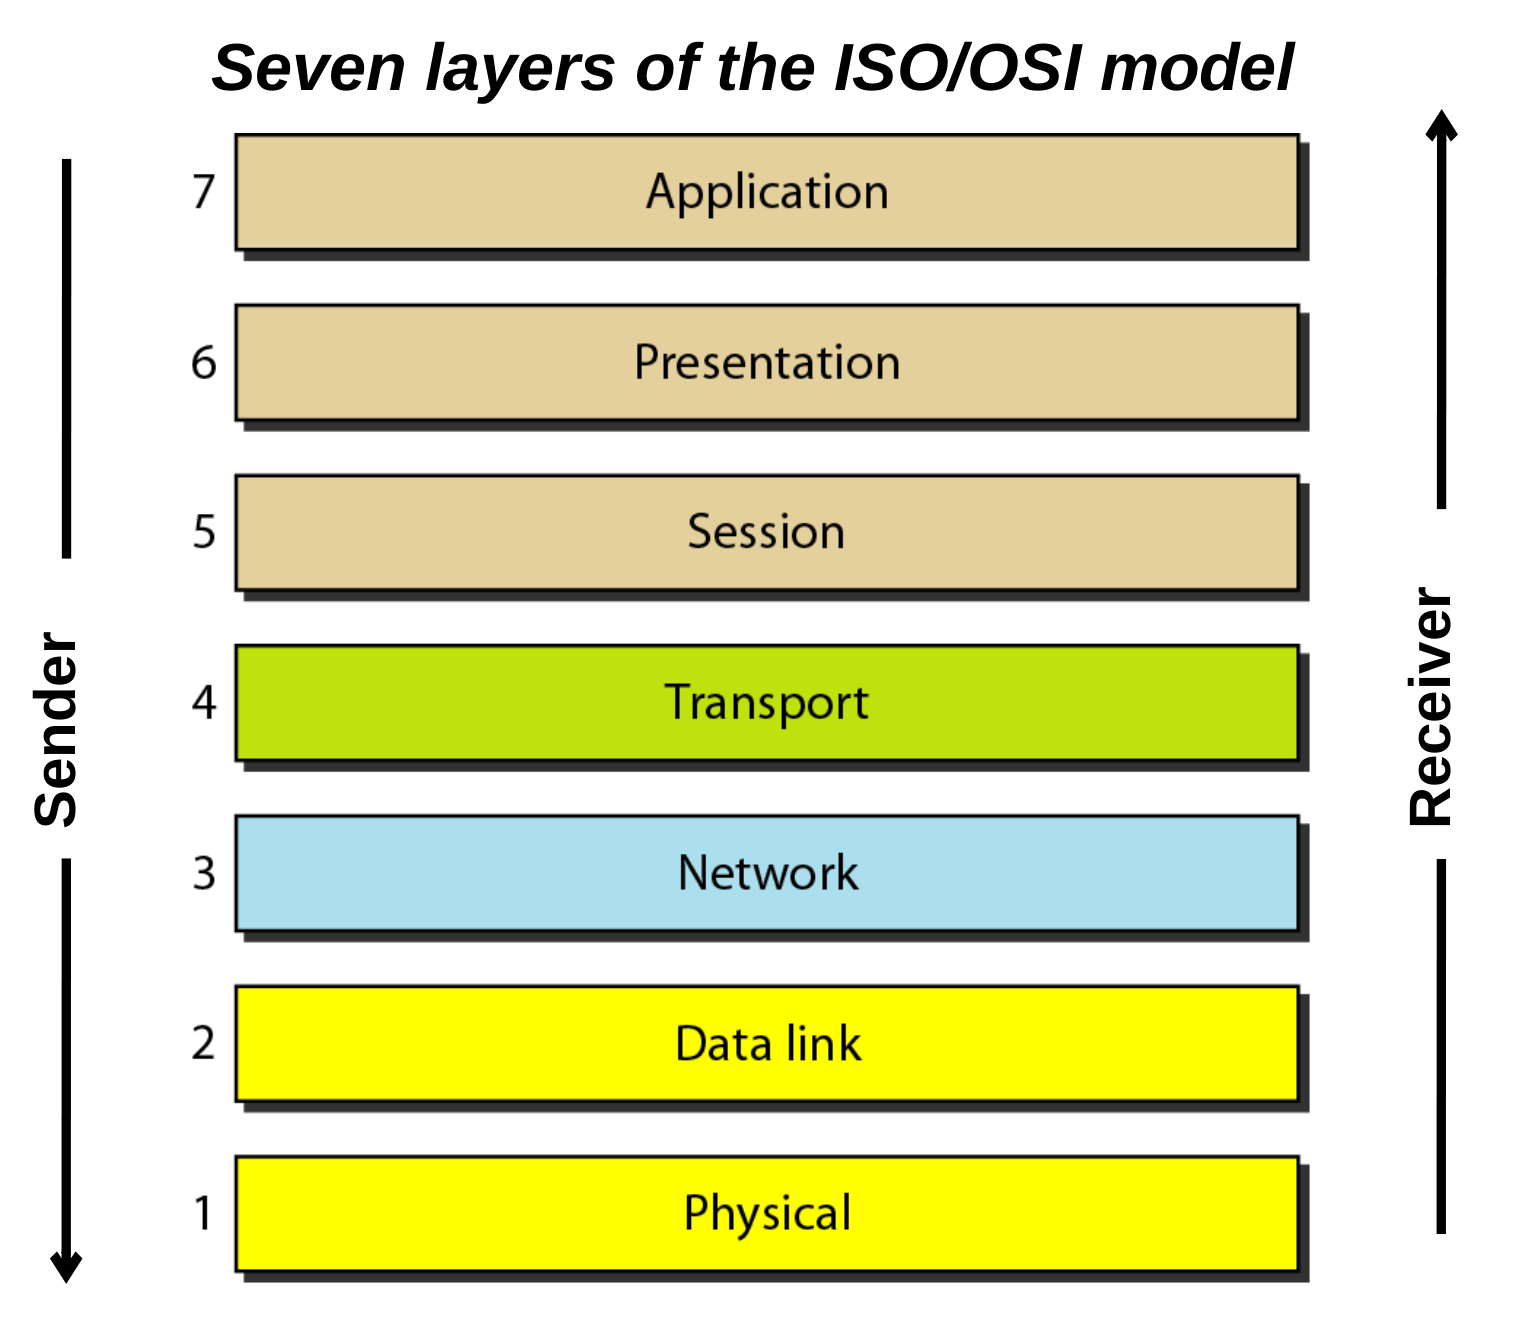
\includegraphics[width=\linewidth]{cap02/osi_sette_strati.png}
\end{minipage}\hfill
\begin{minipage}{0.54\linewidth}
\begin{itemize}
  \item \textbf{Sette strati}, ciascuno creato dove serviva un'\textbf{astrazione diversa}.
  \item Il suo contributo più importante è aver reso \textbf{servizi}, \textbf{interfacce} e
        \textbf{protocolli} tre concetti \textbf{esplicitamente separati}.
  \item Il mittente scende lungo la pila, il destinatario la risale.
\end{itemize}
\end{minipage}
\caption{I sette strati del modello ISO/OSI.}
\end{figure}

\begin{table}[H]
\centering
\begin{tabular}{clp{9.5cm}}
\toprule
\textbf{\#} & \textbf{Strato} & \textbf{Compito} \\
\midrule
7 & Applicazione & servizi all'utente: login remoto, trasferimento file, posta, Web \\
6 & Presentazione & rappresentazione dei dati: traduzione tra codifiche, cifratura, compressione \\
5 & Sessione & controllo del dialogo (chi parla, quando e per quanto) e checkpoint \\
4 & Trasporto & consegna end-to-end al processo giusto (porte), segmentazione, controllo di flusso e degli errori \\
3 & Rete & consegna dei pacchetti dall'host sorgente all'host destinazione: indirizzamento logico e routing \\
2 & Collegamento & consegna dei frame da un nodo al successivo (un hop), controllo degli errori e accesso al mezzo \\
1 & Fisico & trasmissione dei singoli bit sul mezzo \\
\bottomrule
\end{tabular}
\caption{I sette strati OSI, dall'alto verso il basso.}
\end{table}

\info{Un trucco mnemonico}{
    Dal basso verso l'alto: \textbf{F}isico, \textbf{C}ollegamento, \textbf{R}ete, \textbf{T}rasporto,
    \textbf{S}essione, \textbf{P}resentazione, \textbf{A}pplicazione. In inglese si usa la frase
    ``\emph{\textbf{P}lease \textbf{D}o \textbf{N}ot \textbf{T}hrow \textbf{S}ausage \textbf{P}izza
    \textbf{A}way}'' (Physical, Data link, Network, Transport, Session, Presentation, Application).
}

\subsection{Non tutti i nodi implementano tutti gli strati}

\begin{figure}[H]
    \centering
    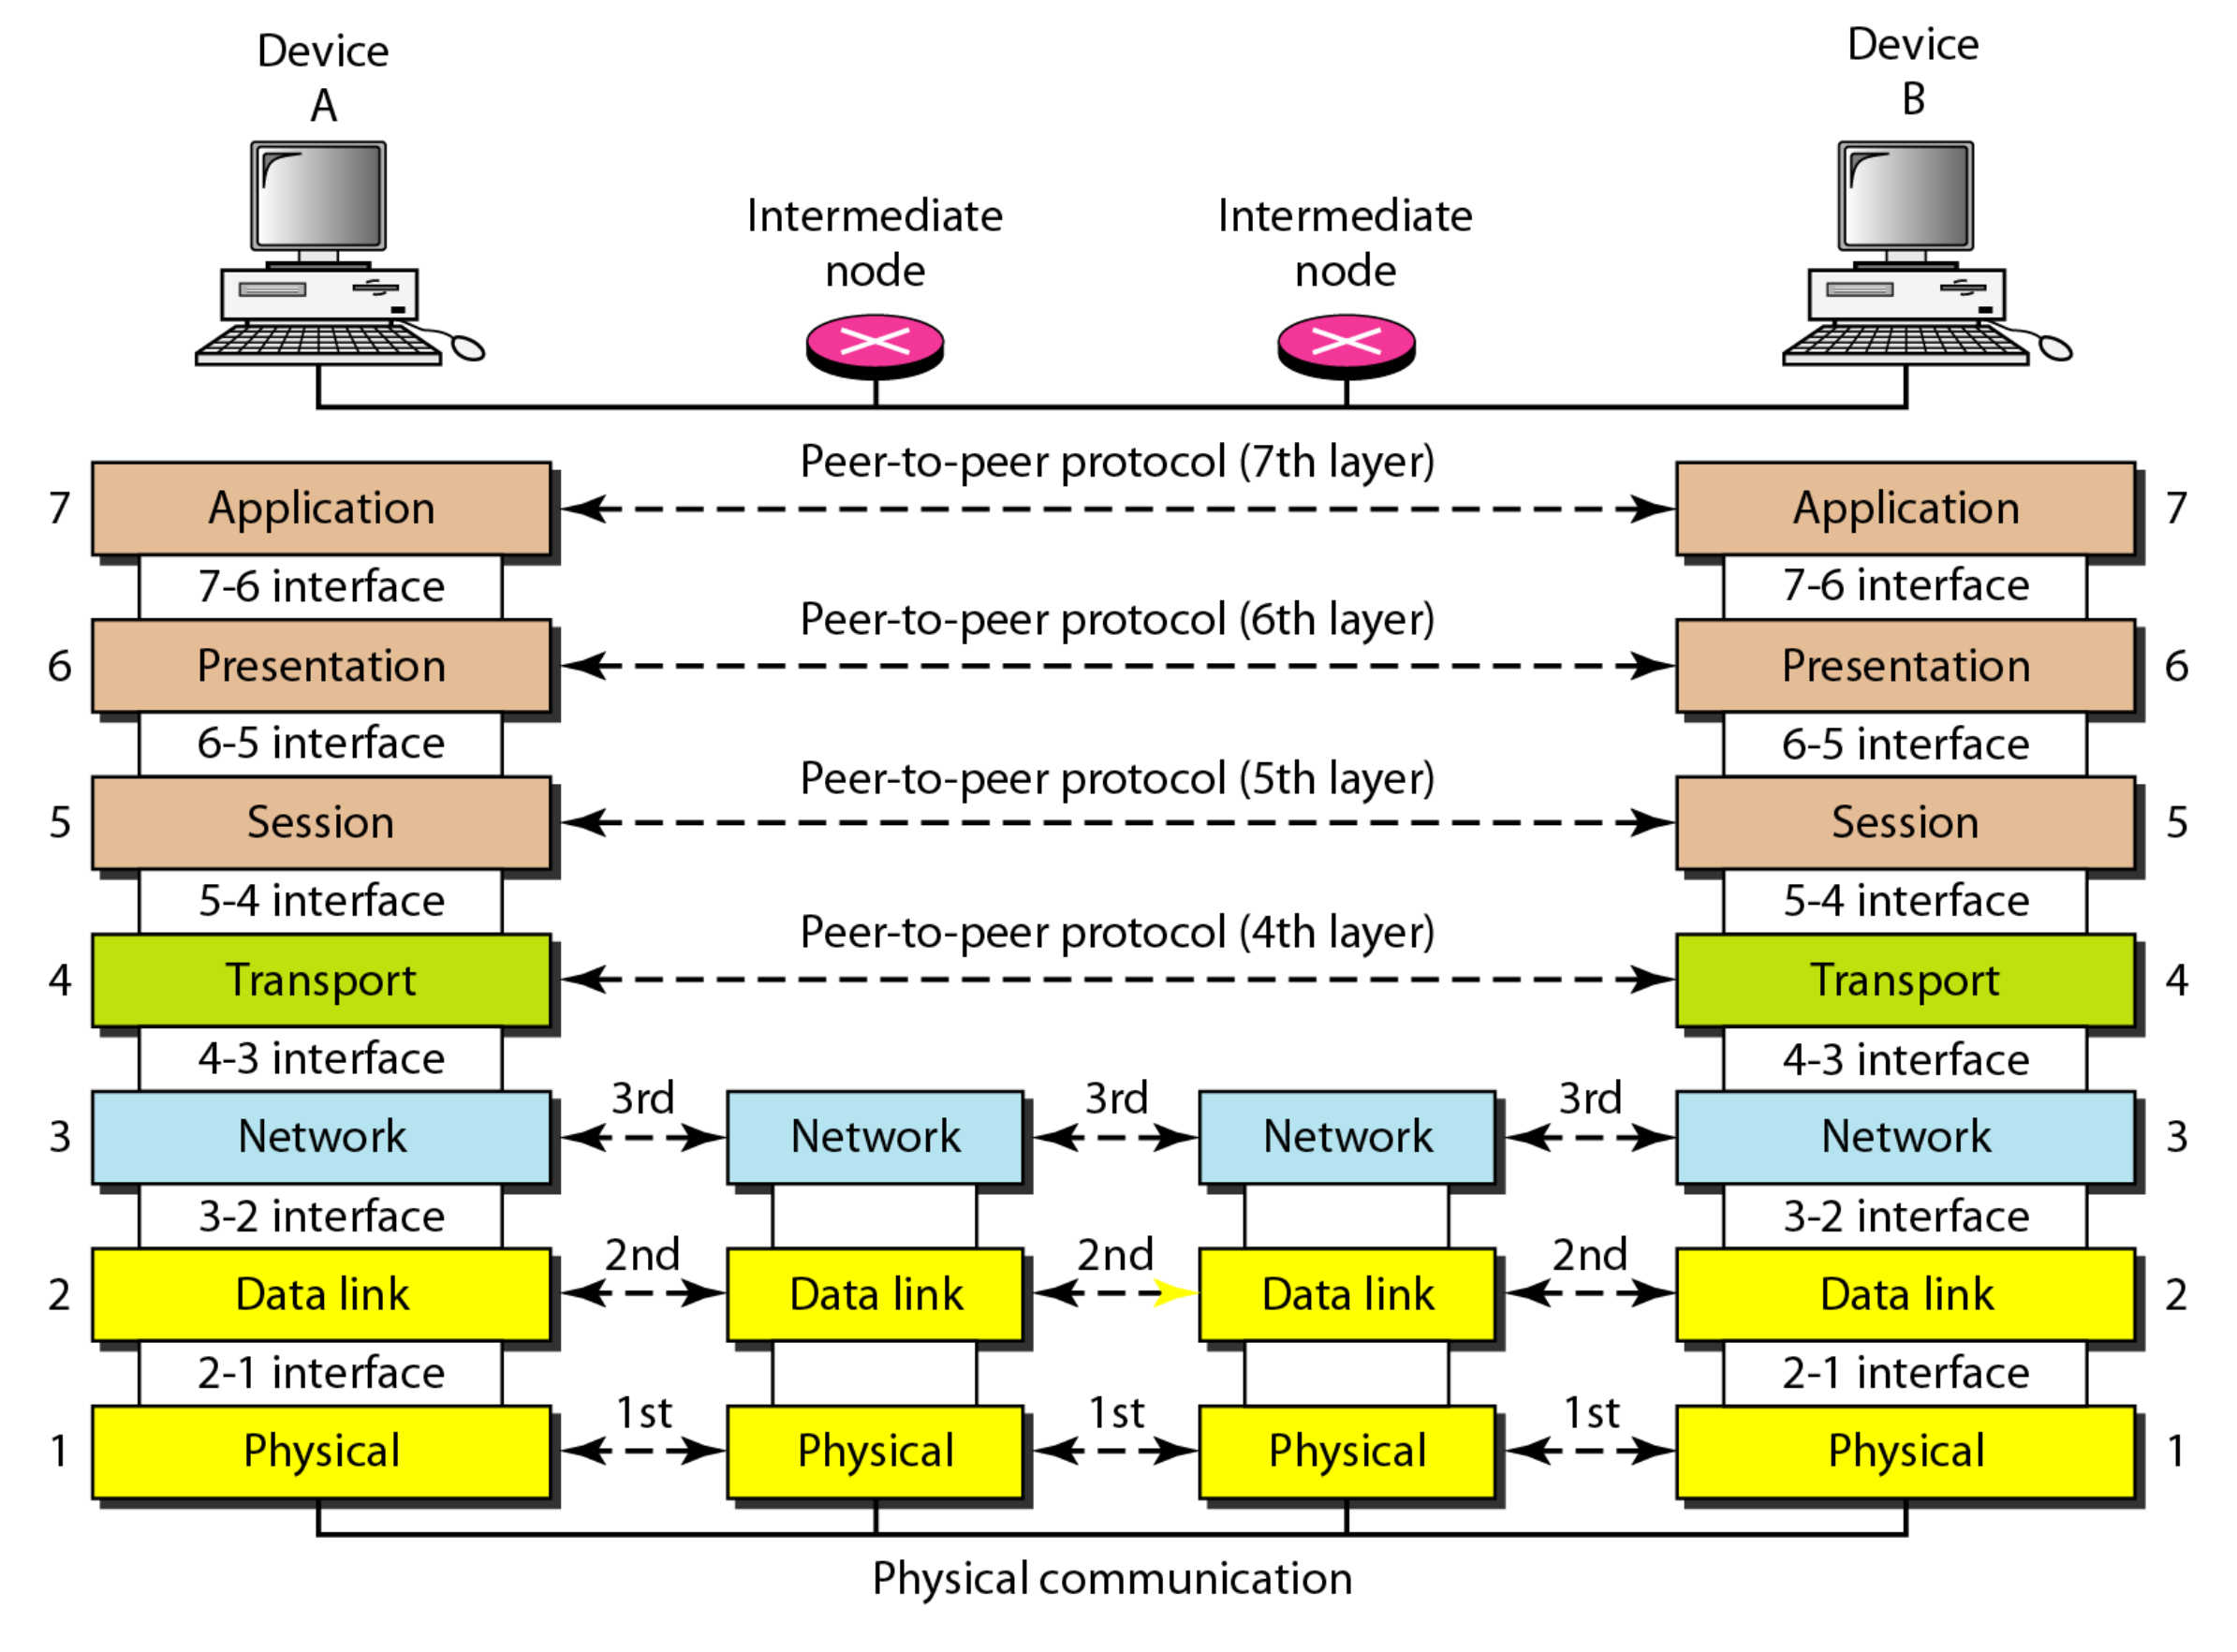
\includegraphics[width=0.72\linewidth]{cap02/osi_nodi_intermedi.png}
    \caption{I nodi intermedi implementano solo i primi tre strati; solo gli host implementano l'intera pila.}
\end{figure}

\begin{itemize}
    \item Solo i \textbf{sistemi terminali} (host) implementano l'intera pila, fino all'applicazione.
    \item I \textbf{nodi intermedi} (switch, router) implementano solo due o tre strati, i cosiddetti
          \emph{media layer}.
    \item Niente sopra il livello di rete: un router non ha alcun motivo di leggere il vostro messaggio.
\end{itemize}

\warning{Trasporto e rete: dove gira il software}{
    A livello di \textbf{trasporto} la comunicazione è tra \textbf{processi}, dal punto di vista logico è
    punto-punto, e il software è eseguito \textbf{sugli host}. A livello di \textbf{rete} la comunicazione
    è tra \textbf{host}: si risolve il problema dell'instradamento dei pacchetti attraverso la
    topologia della rete, e il software è eseguito prevalentemente \textbf{sui nodi della rete}. Un
    router non ha bisogno del trasporto perché non gli interessa a quale processo sia destinato il
    pacchetto: gli basta sapere a quale host deve arrivare.
}

% ══════════════════════════════════════════════════════════════
\section{Incapsulamento e decapsulamento}
% ══════════════════════════════════════════════════════════════

\begin{figure}[H]
    \centering
    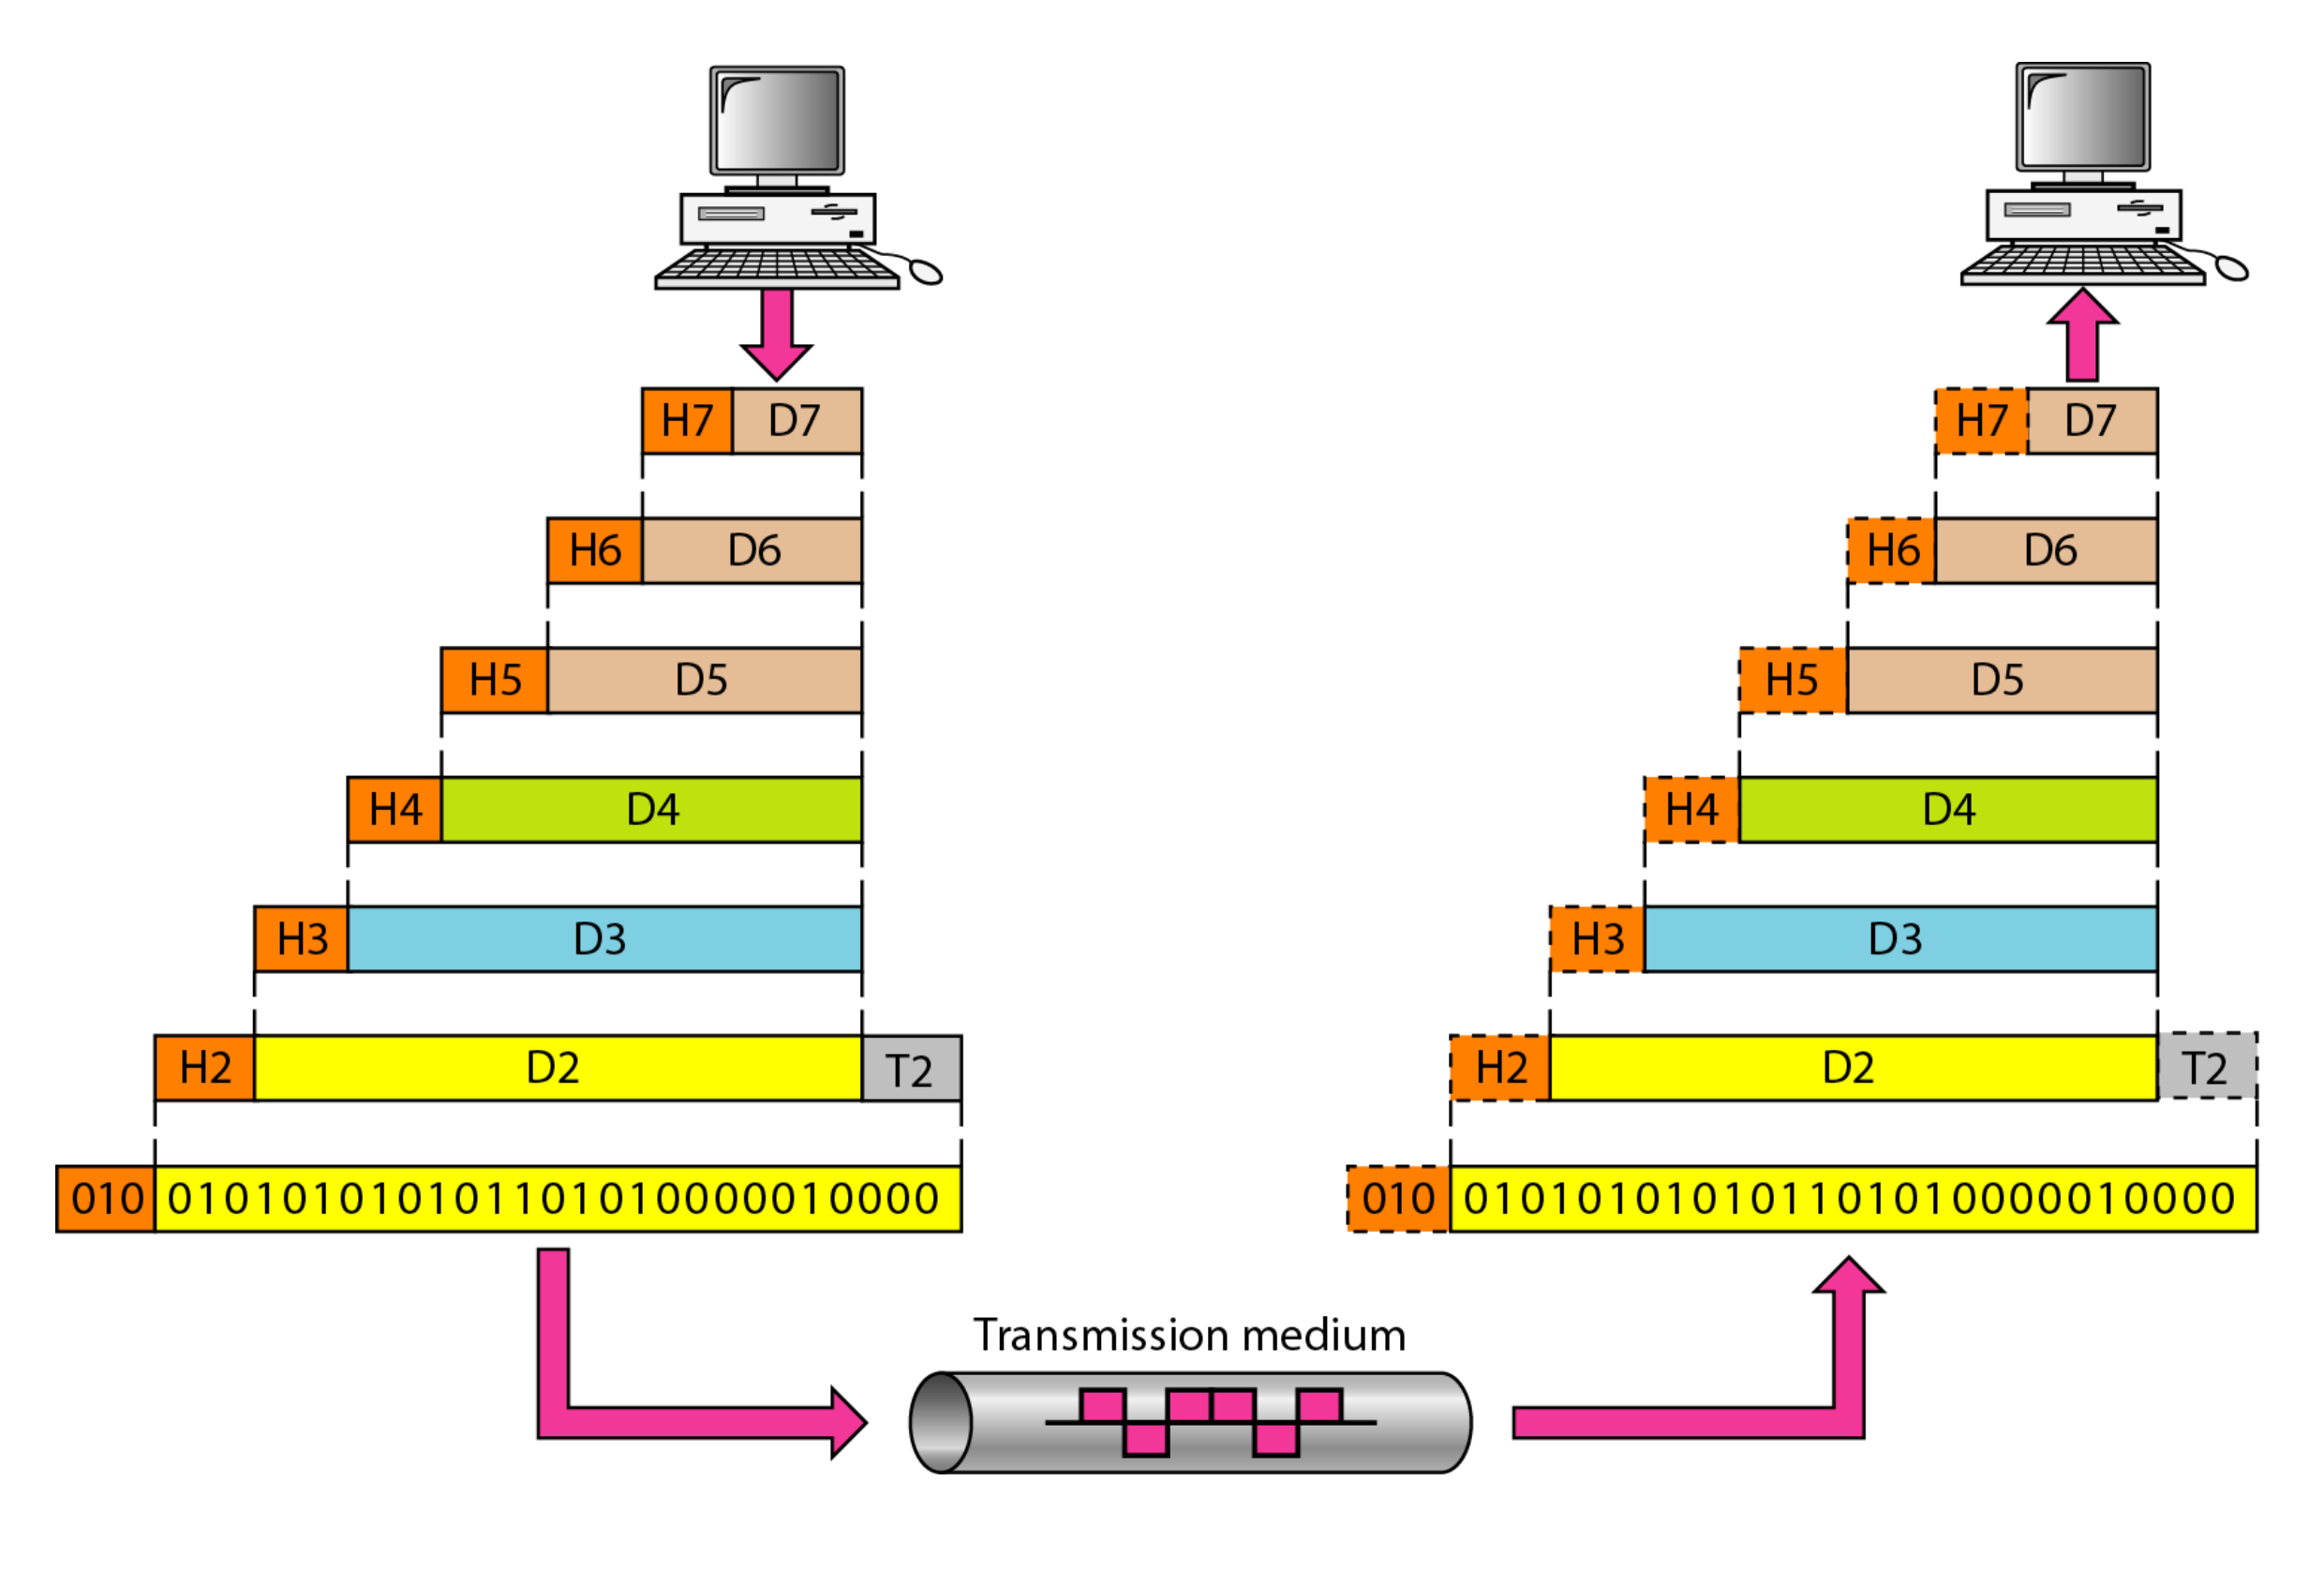
\includegraphics[width=0.7\linewidth]{cap02/incapsulamento.png}
    \caption{Ogni strato del mittente aggiunge un header (e a volte un trailer); ogni strato del destinatario toglie il proprio.}
\end{figure}

\dfn{Incapsulamento e decapsulamento}{
    \begin{itemize}
      \item \textbf{Incapsulamento} (scendendo, \emph{top-down}): ogni strato del mittente aggiunge a ciò
            che riceve dallo strato superiore un proprio campo di controllo, sotto forma di un
            \textbf{header} (H) in testa e talvolta di un \textbf{trailer} (T) in coda.
      \item \textbf{Decapsulamento} (salendo, \emph{bottom-up}): ogni strato del destinatario rimuove e
            interpreta \textbf{esattamente} il campo aggiunto dal suo pari, e passa il resto verso l'alto.
    \end{itemize}
    Un'unità di dati, a qualunque strato, è quindi sempre \textbf{header + payload}, e il
    \textbf{payload} è l'unità dello strato superiore.
}

\begin{figure}[H]
\centering
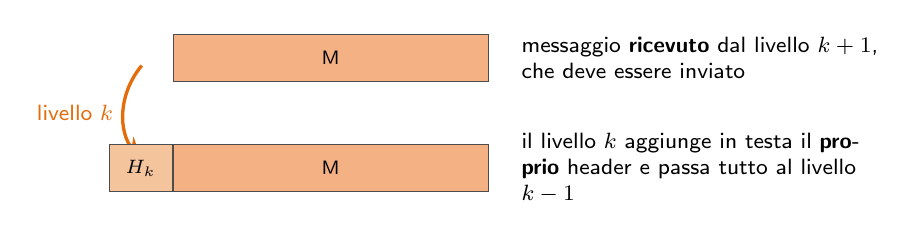
\begin{tikzpicture}[every node/.style={font=\footnotesize\sffamily}]
  \node[field, fill=lapp, minimum width=4cm, minimum height=0.6cm] (m) at (0,0) {M};
  \node[anchor=west, lbl, text width=4.6cm, align=left] at (2.3,0) {messaggio \textbf{ricevuto} dal livello $k+1$, che deve essere inviato};
  \draw[-{Stealth}, very thick, netorange] (-2.4,-0.1) to[bend right=40] node[left, lbl] {livello $k$} (-2.4,-1.3);
  \node[field, fill=lapp, minimum width=4cm, minimum height=0.6cm] (m2) at (0,-1.4) {M};
  \node[field, fill=netorange!40, minimum width=0.8cm, minimum height=0.6cm, left=0pt of m2] {$H_k$};
  \node[anchor=west, lbl, text width=4.6cm, align=left] at (2.3,-1.4) {il livello $k$ aggiunge in testa il \textbf{proprio} header e passa tutto al livello $k-1$};
\end{tikzpicture}
\caption{Il passo elementare dell'incapsulamento, come alla lavagna: $M$ arriva dall'alto e diventa il payload di $H_k + M$.}
\end{figure}

\begin{figure}[H]
\centering
\begin{tikzpicture}[every node/.style={font=\scriptsize\sffamily}]
  % mittente
  \node[font=\small\bfseries\sffamily] at (2.2,1.6) {Mittente};
  \node[field, fill=lapp, minimum width=2cm] (m1) at (2.6,0) {M};
  \node[field, fill=ltra, minimum width=0.6cm, left=0pt of m1] (ht) {$H_t$};
  \node[field, fill=lapp, minimum width=2cm] (m2) at (2.6,-0.9) {M};
  \node[field, fill=ltra, minimum width=0.6cm, left=0pt of m2] (ht2) {$H_t$};
  \node[field, fill=lnet, minimum width=0.6cm, left=0pt of ht2] (hn2) {$H_n$};
  \node[field, fill=lapp, minimum width=2cm] (m3) at (2.6,-1.8) {M};
  \node[field, fill=ltra, minimum width=0.6cm, left=0pt of m3] (ht3) {$H_t$};
  \node[field, fill=lnet, minimum width=0.6cm, left=0pt of ht3] (hn3) {$H_n$};
  \node[field, fill=llink, minimum width=0.6cm, left=0pt of hn3] (hl3) {$H_l$};
  \node[field, fill=llink, minimum width=0.6cm, right=0pt of m3] (tl3) {$T_l$};
  \node[field, fill=lapp, minimum width=2cm, draw=none] (m0) at (2.6,0.9) {};
  % labels levels
  \foreach \y/\t/\u in {0.9/Applicazione/messaggio, 0/Trasporto/segmento, -0.9/Rete/datagramma, -1.8/Collegamento/frame, -2.7/Fisico/bit} {
     \node[anchor=east] at (-0.8,\y) {\t};
     \node[anchor=west, text=primary] at (4.4,\y) {\u};
  }
  \node[field, fill=lapp, minimum width=2cm] at (2.6,0.9) {M};
  \node at (2.2,-2.7) {0110100101110\dots};
  \draw[-{Stealth}, thick, netred] (-0.3,1.1) -- (-0.3,-2.9);
  % destinatario
  \begin{scope}[xshift=8.5cm]
    \node[font=\small\bfseries\sffamily] at (2.2,1.6) {Destinatario};
    \node[field, fill=lapp, minimum width=2cm] at (2.6,0.9) {M};
    \node[field, fill=lapp, minimum width=2cm] (d1) at (2.6,0) {M};
    \node[field, fill=ltra, minimum width=0.6cm, left=0pt of d1] {$H_t$};
    \node[field, fill=lapp, minimum width=2cm] (d2) at (2.6,-0.9) {M};
    \node[field, fill=ltra, minimum width=0.6cm, left=0pt of d2] (e2) {$H_t$};
    \node[field, fill=lnet, minimum width=0.6cm, left=0pt of e2] {$H_n$};
    \node[field, fill=lapp, minimum width=2cm] (d3) at (2.6,-1.8) {M};
    \node[field, fill=ltra, minimum width=0.6cm, left=0pt of d3] (e3) {$H_t$};
    \node[field, fill=lnet, minimum width=0.6cm, left=0pt of e3] (f3) {$H_n$};
    \node[field, fill=llink, minimum width=0.6cm, left=0pt of f3] {$H_l$};
    \node[field, fill=llink, minimum width=0.6cm, right=0pt of d3] {$T_l$};
    \node at (2.2,-2.7) {0110100101110\dots};
    \draw[-{Stealth}, thick, netgreen] (4.6,-2.9) -- (4.6,1.1);
  \end{scope}
  \draw[-{Stealth}, very thick, black!60, decorate, decoration={snake, amplitude=1.2pt, segment length=6pt, post length=2mm}] (5.4,-2.7) -- node[below=3pt] {mezzo fisico} (9.5,-2.7);
\end{tikzpicture}
\caption{Incapsulamento nella pila a cinque strati: ogni strato tratta tutto ciò che riceve dall'alto come un blocco unico a cui aggiungere il proprio header.}
\end{figure}

\subsection{Sotto il proprio strato, il payload è opaco}

Quando il messaggio di livello 7 scende, tutto ciò che viene dall'alto (header e contenuto insieme)
diventa il \textbf{payload} del livello 6.

\begin{itemize}
    \item Il livello 6 aggiunge il proprio header e passa tutto al livello 5, che fa lo stesso, e così via.
    \item Il livello 6 \textbf{non sa} di trasportare HTML, e non deve interessargli: per lui il payload è
          una \textbf{sequenza di byte opaca}.
    \item È proprio questo che rende gli strati \textbf{indipendenti}: uno strato che ispezionasse il
          proprio payload smetterebbe di funzionare appena cambia lo strato superiore.
\end{itemize}

Il destinatario ripercorre la sequenza al contrario, e ogni strato toglie soltanto il proprio header.

\info{Lo tocchiamo con mano}{
    Quando nel capitolo sui socket scriveremo a mano una richiesta HTTP, vedremo che un messaggio a
    livello di applicazione viene semplicemente inviato come \textbf{payload} di un messaggio di
    trasporto, il cui contenuto è del tutto irrilevante (``trasparente'') per il livello di trasporto.
}

% ══════════════════════════════════════════════════════════════
\section{I sette strati, uno per uno}
% ══════════════════════════════════════════════════════════════

\subsection{1. Livello fisico (Physical)}

\begin{figure}[H]
\centering
\begin{minipage}{0.48\linewidth}\centering
  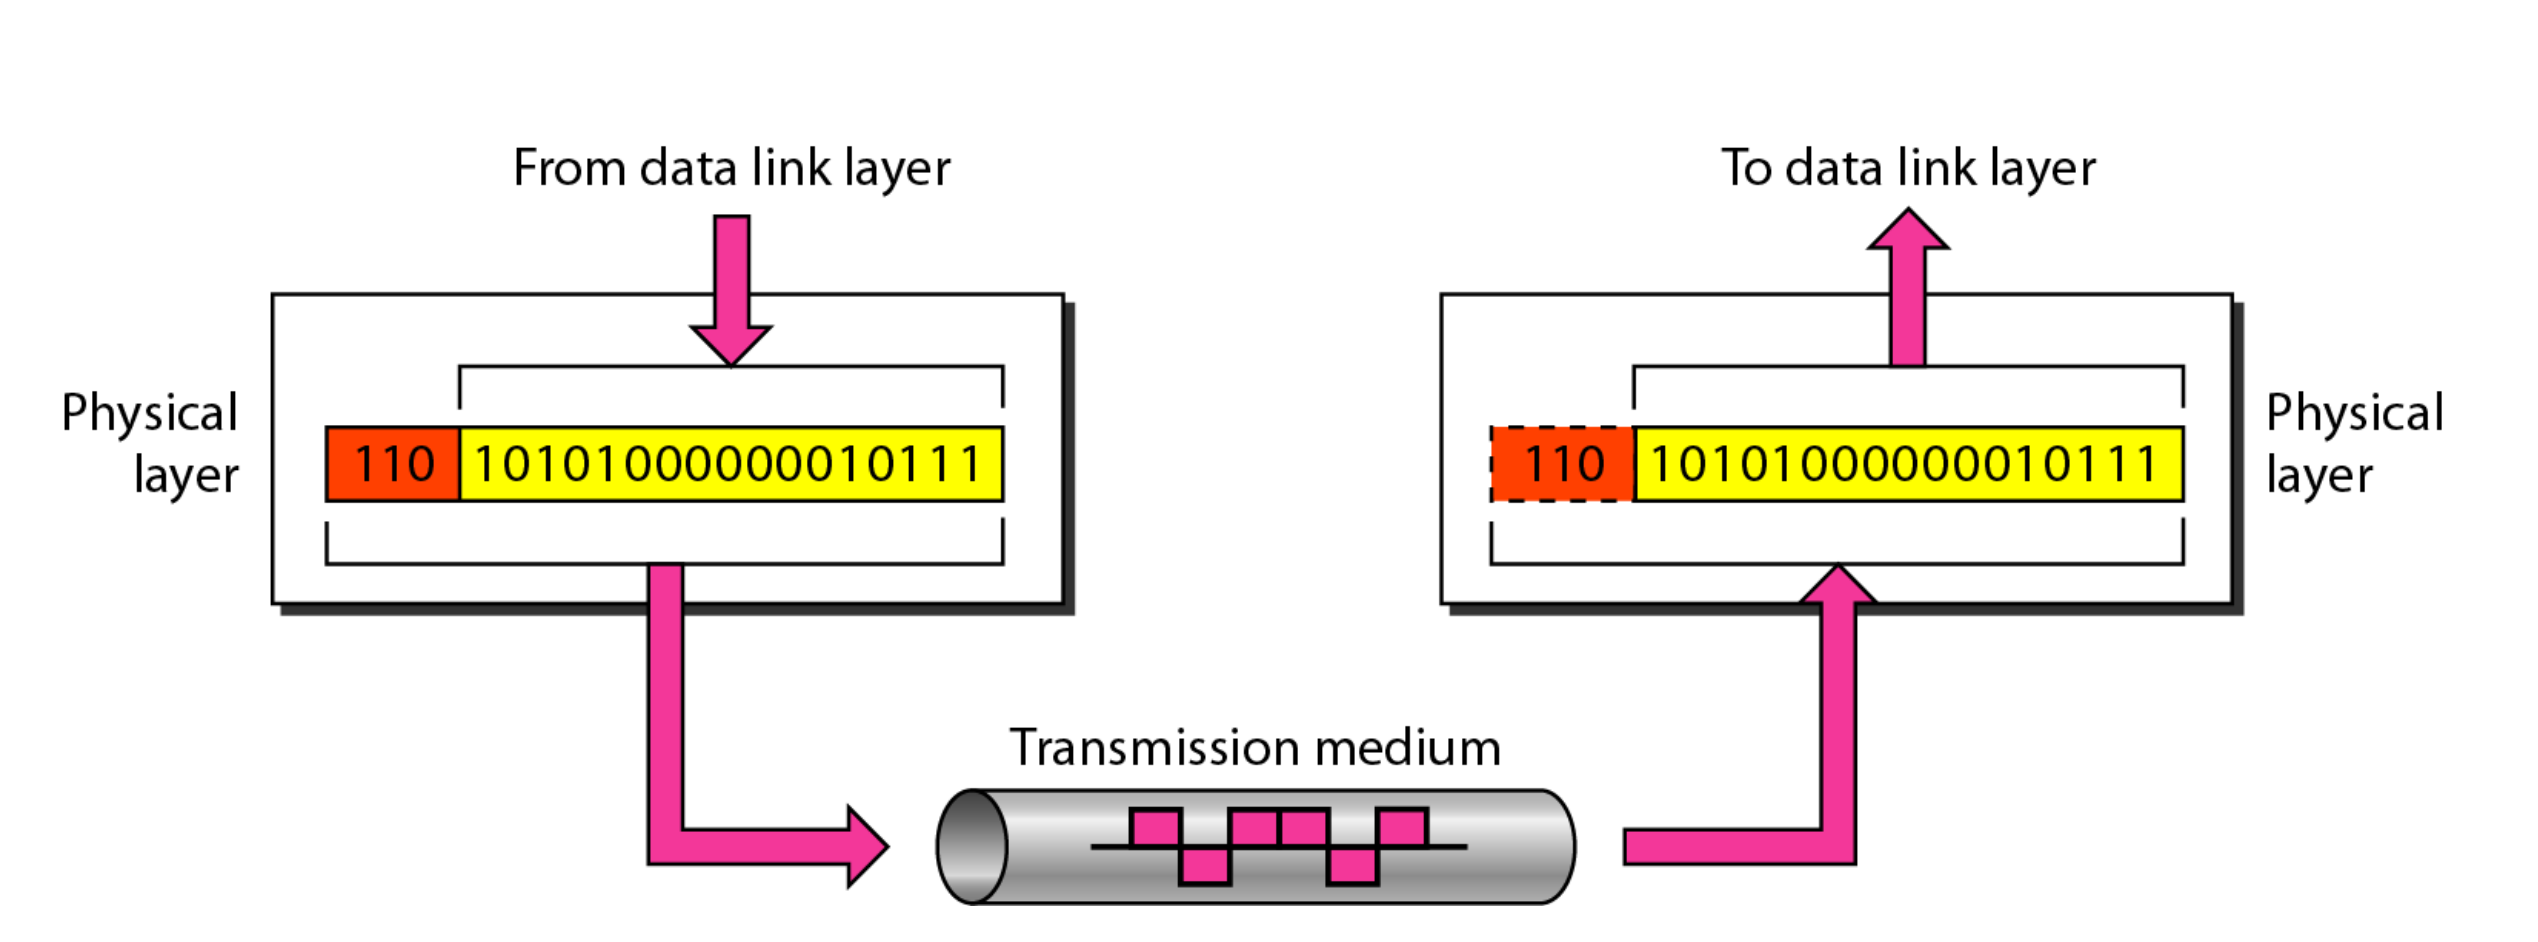
\includegraphics[width=\linewidth]{cap02/osi_fisico.png}
\end{minipage}\hfill
\begin{minipage}{0.48\linewidth}
È responsabile di \textbf{spostare i singoli bit} da un nodo al successivo lungo il mezzo. Si occupa di:
\begin{itemize}
  \item caratteristiche fisiche di interfacce e mezzi (connettori, cavi, segnali elettrici);
  \item configurazione della linea (punto-punto o multipunto) e topologia fisica;
  \item modalità di trasmissione (simplex, half-duplex, full-duplex);
  \item rappresentazione dei bit, velocità (data rate) e sincronizzazione dei bit tra i due estremi.
\end{itemize}
\end{minipage}
\end{figure}

\begin{figure}[H]
\centering
\begin{tikzpicture}[every node/.style={font=\footnotesize\sffamily}]
  \node (t1) at (0,0.9) {\icon[0.8cm]{pc}}; \node[above=-1pt of t1, text=netblue, font=\small\bfseries\sffamily] {T1};
  \node (t2) at (10,0.9) {\icon[0.8cm]{pc}}; \node[above=-1pt of t2, text=netblue, font=\small\bfseries\sffamily] {T2};
  \node[font=\ttfamily\footnotesize, text=netblue] (b1) at (0,0) {0001100110000110};
  \node[font=\ttfamily\footnotesize, text=netblue] (b2) at (10,0) {0001100110000110};
  \node[draw, fill=lphy, minimum width=1.2cm, minimum height=0.5cm] (p1) at (1.2,-1) {PHYS};
  \node[draw, fill=lphy, minimum width=1.2cm, minimum height=0.5cm] (p2) at (8.8,-1) {PHYS};
  \node[cylinder, shape border rotate=0, draw, thick, fill=black!5, aspect=0.25, minimum height=4.8cm, minimum width=0.55cm] (c) at (5,-1) {};
  \node[below=2pt of c, lbl] {mezzo fisico: cavo, fibra, onde radio};
  \draw[-{Stealth}, thick, netorange] (b1.south) to[bend right=20] (p1.north);
  \draw[-{Stealth}, thick, netorange] (p1) -- (c.west);
  \draw[-{Stealth}, thick, netorange] (c.east) -- (p2);
  \draw[-{Stealth}, thick, netorange] (p2.north) to[bend right=20] (b2.south);
  \foreach \x in {3.3,3.9,4.5,5.1,5.7,6.3} \draw[netorange!80!black, thick, decorate, decoration={snake, amplitude=1.2pt, segment length=4pt}] (\x,-1) -- ++(0.4,0);
\end{tikzpicture}
\caption{Il livello fisico: la sequenza di bit di T1 diventa un segnale sul mezzo e ricompare identica (se tutto va bene) in T2.}
\end{figure}

\subsection{2. Livello di collegamento (Data Link)}

\begin{figure}[H]
\centering
\begin{minipage}{0.48\linewidth}\centering
  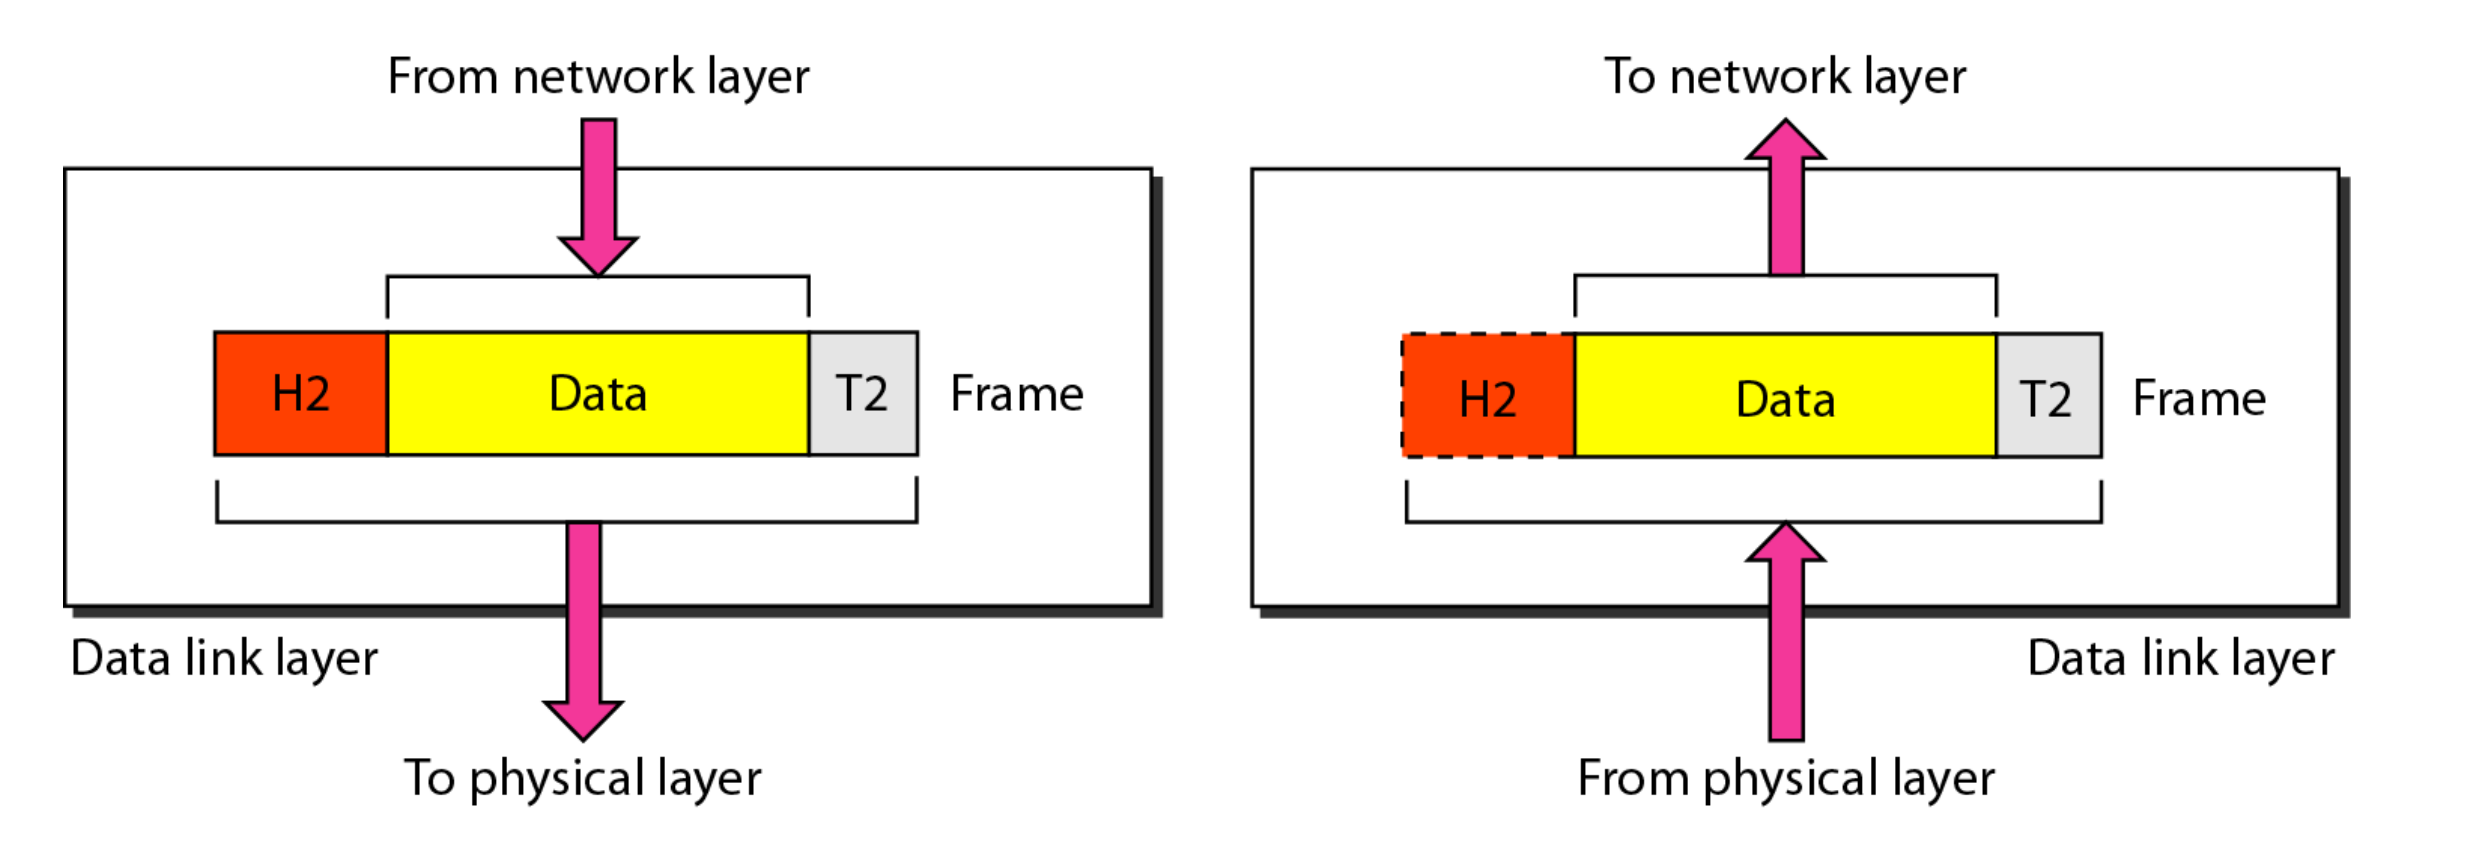
\includegraphics[width=\linewidth]{cap02/osi_collegamento.png}
\end{minipage}\hfill
\begin{minipage}{0.48\linewidth}
È responsabile di \textbf{spostare i frame da un nodo al successivo}: un solo salto (\emph{hop}),
non l'intero cammino. Si occupa di:
\begin{itemize}
  \item organizzare i dati in \textbf{frame}, blocchi di dimensione limitata (tipicamente qualche
        centinaio di byte), con header $H_2$ e trailer $T_2$;
  \item \textbf{controllo di flusso} e \textbf{controllo degli errori}, tramite la \emph{frame check
        sequence} (FCS) nel trailer;
  \item \textbf{controllo dell'accesso} al mezzo quando è condiviso.
\end{itemize}
\end{minipage}
\end{figure}

\dfn{Sottostrato MAC}{
    Il livello di collegamento contiene il \textbf{sottostrato MAC} (\emph{Medium Access Control}), che si occupa
    della \textbf{gestione dell'accesso a un unico mezzo di trasmissione} da parte di più stazioni \textbf{in
    competizione} tra loro. Ethernet ne è l'esempio più noto.
}

\subsection{3. Livello di rete (Network)}

\begin{figure}[H]
\centering
\begin{minipage}{0.48\linewidth}\centering
  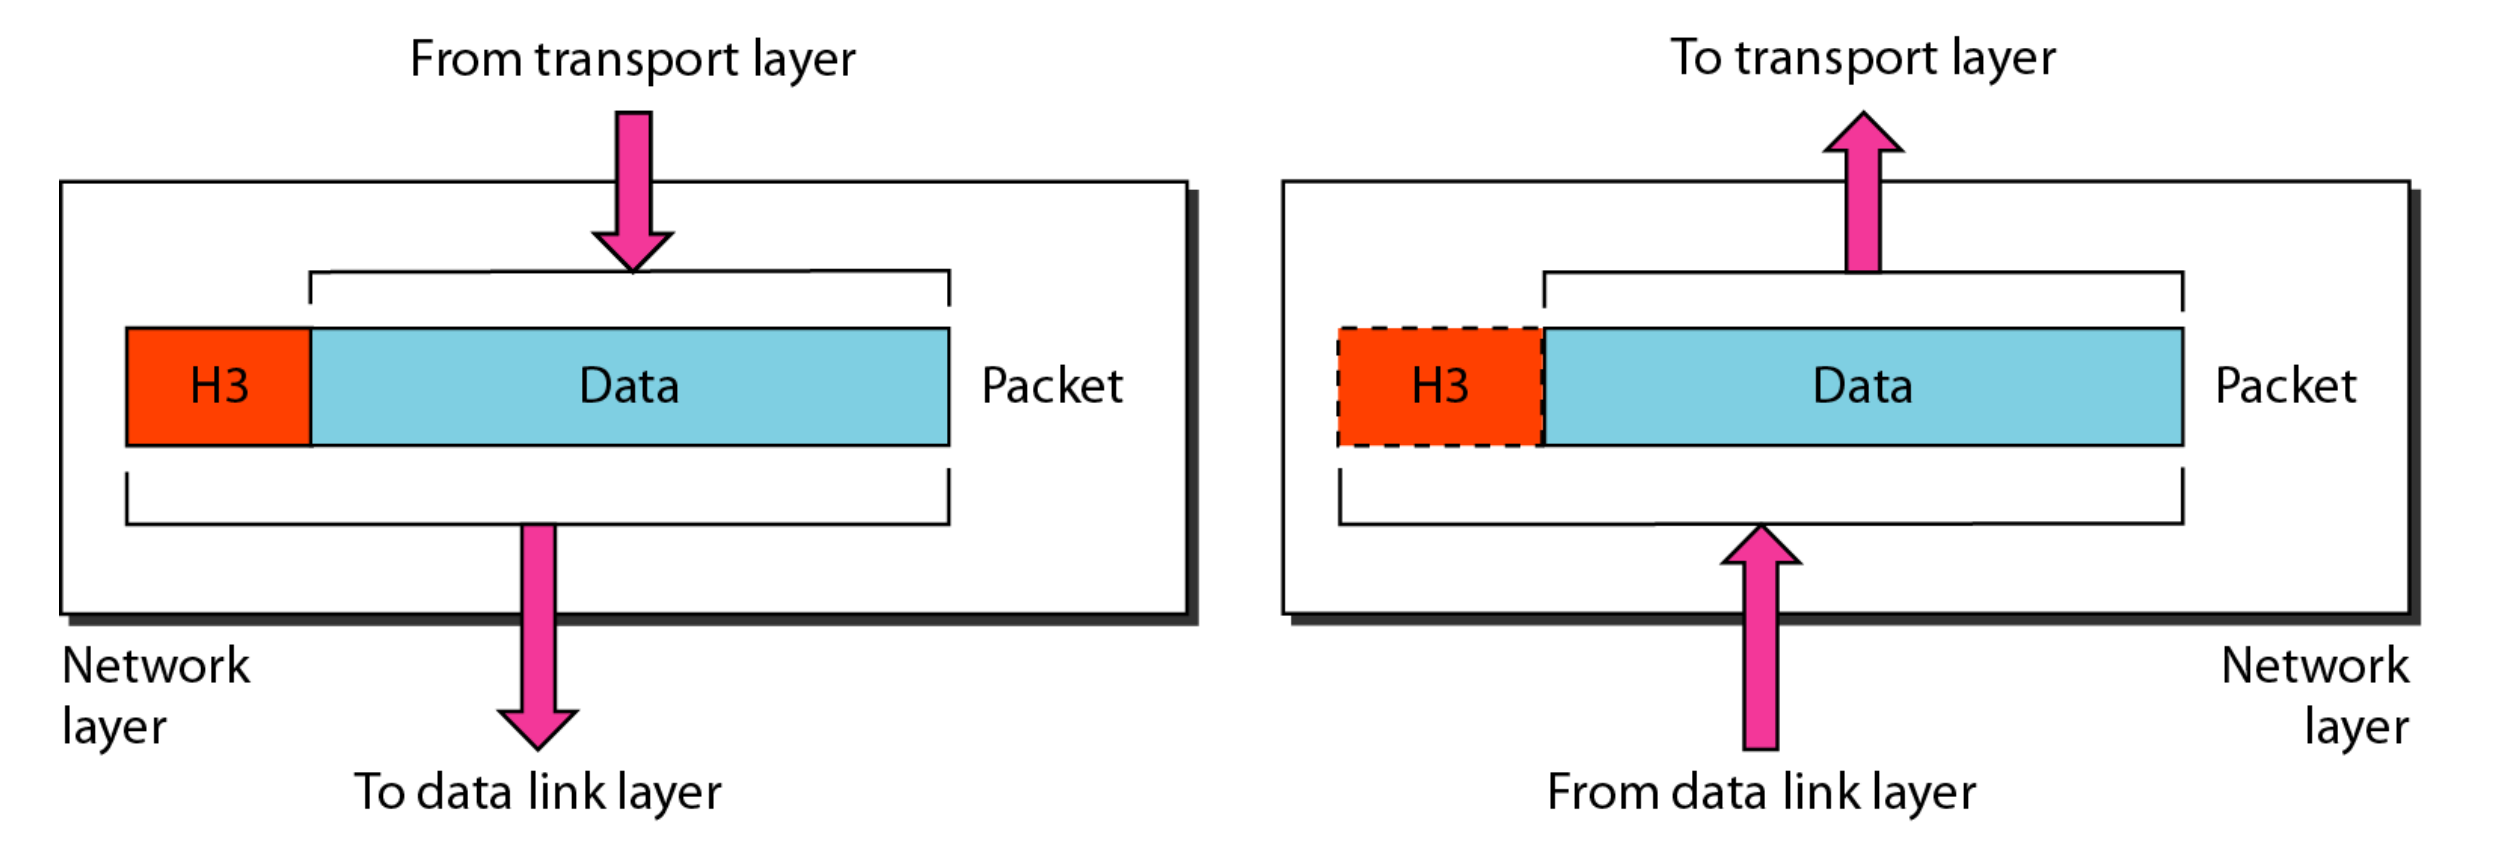
\includegraphics[width=\linewidth]{cap02/osi_rete.png}
\end{minipage}\hfill
\begin{minipage}{0.48\linewidth}
È responsabile di \textbf{consegnare i pacchetti dall'host sorgente all'host destinazione}, lungo
l'intero cammino. Si occupa di:
\begin{itemize}
  \item attraversare la \textbf{topologia}: la rete è un grafo di nodi con più di una strada possibile;
  \item \textbf{indirizzamento logico} (gli indirizzi IP);
  \item \textbf{routing}: decidere, nodo per nodo, da quale collegamento far uscire il pacchetto
        (tabelle di instradamento).
\end{itemize}
\end{minipage}
\end{figure}

\begin{figure}[H]
\centering
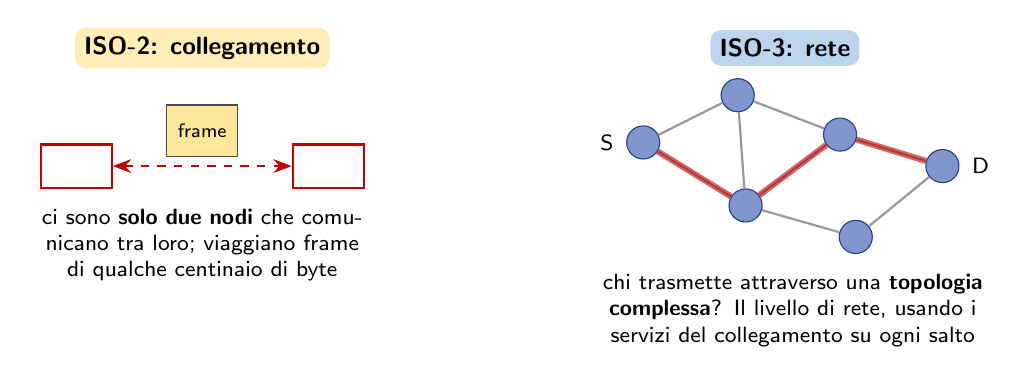
\begin{tikzpicture}[every node/.style={font=\footnotesize\sffamily}]
  \begin{scope}
    \node[font=\small\bfseries\sffamily, fill=llink!70, rounded corners] at (1.6,1.5) {ISO-2: collegamento};
    \node[draw=netred, thick, minimum width=0.9cm, minimum height=0.55cm] (a) at (0,0) {};
    \node[draw=netred, thick, minimum width=0.9cm, minimum height=0.55cm] (b) at (3.2,0) {};
    \draw[{Stealth}-{Stealth}, dashed, thick, netred] (a) -- (b);
    \node[field, fill=llink, minimum width=0.9cm] at (1.6,0.45) {frame};
    \node[lbl, text width=4.2cm] at (1.6,-1) {ci sono \textbf{solo due nodi} che comunicano tra loro; viaggiano frame di qualche centinaio di byte};
  \end{scope}
  \begin{scope}[xshift=7.2cm]
    \node[font=\small\bfseries\sffamily, fill=lnet!70, rounded corners] at (1.8,1.5) {ISO-3: rete};
    \node[gnode] (s) at (0,0.3) {}; \node[left=1pt of s] {S};
    \node[gnode] (r1) at (1.2,0.9) {}; \node[gnode] (r2) at (1.3,-0.5) {};
    \node[gnode] (r3) at (2.5,0.4) {}; \node[gnode] (r4) at (2.7,-0.9) {};
    \node[gnode] (d) at (3.8,0) {}; \node[right=1pt of d] {D};
    \foreach \x/\y in {s/r1, s/r2, r1/r3, r2/r3, r2/r4, r3/d, r4/d, r1/r2} \draw[black!40, thick] (\x) -- (\y);
    \draw[pathhl, opacity=0.6] (s) -- (r2) -- (r3) -- (d);
    \node[lbl, text width=5.2cm, anchor=north] at (1.9,-1.25) {chi trasmette attraverso una \textbf{topologia complessa}? Il livello di rete, usando i servizi del collegamento su ogni salto};
  \end{scope}
\end{tikzpicture}
\caption{Il collegamento lavora su un solo salto tra due nodi; la rete compone i salti in un cammino dalla sorgente alla destinazione.}
\end{figure}

\subsection{4. Livello di trasporto (Transport)}

\begin{figure}[H]
\centering
\begin{minipage}{0.48\linewidth}\centering
  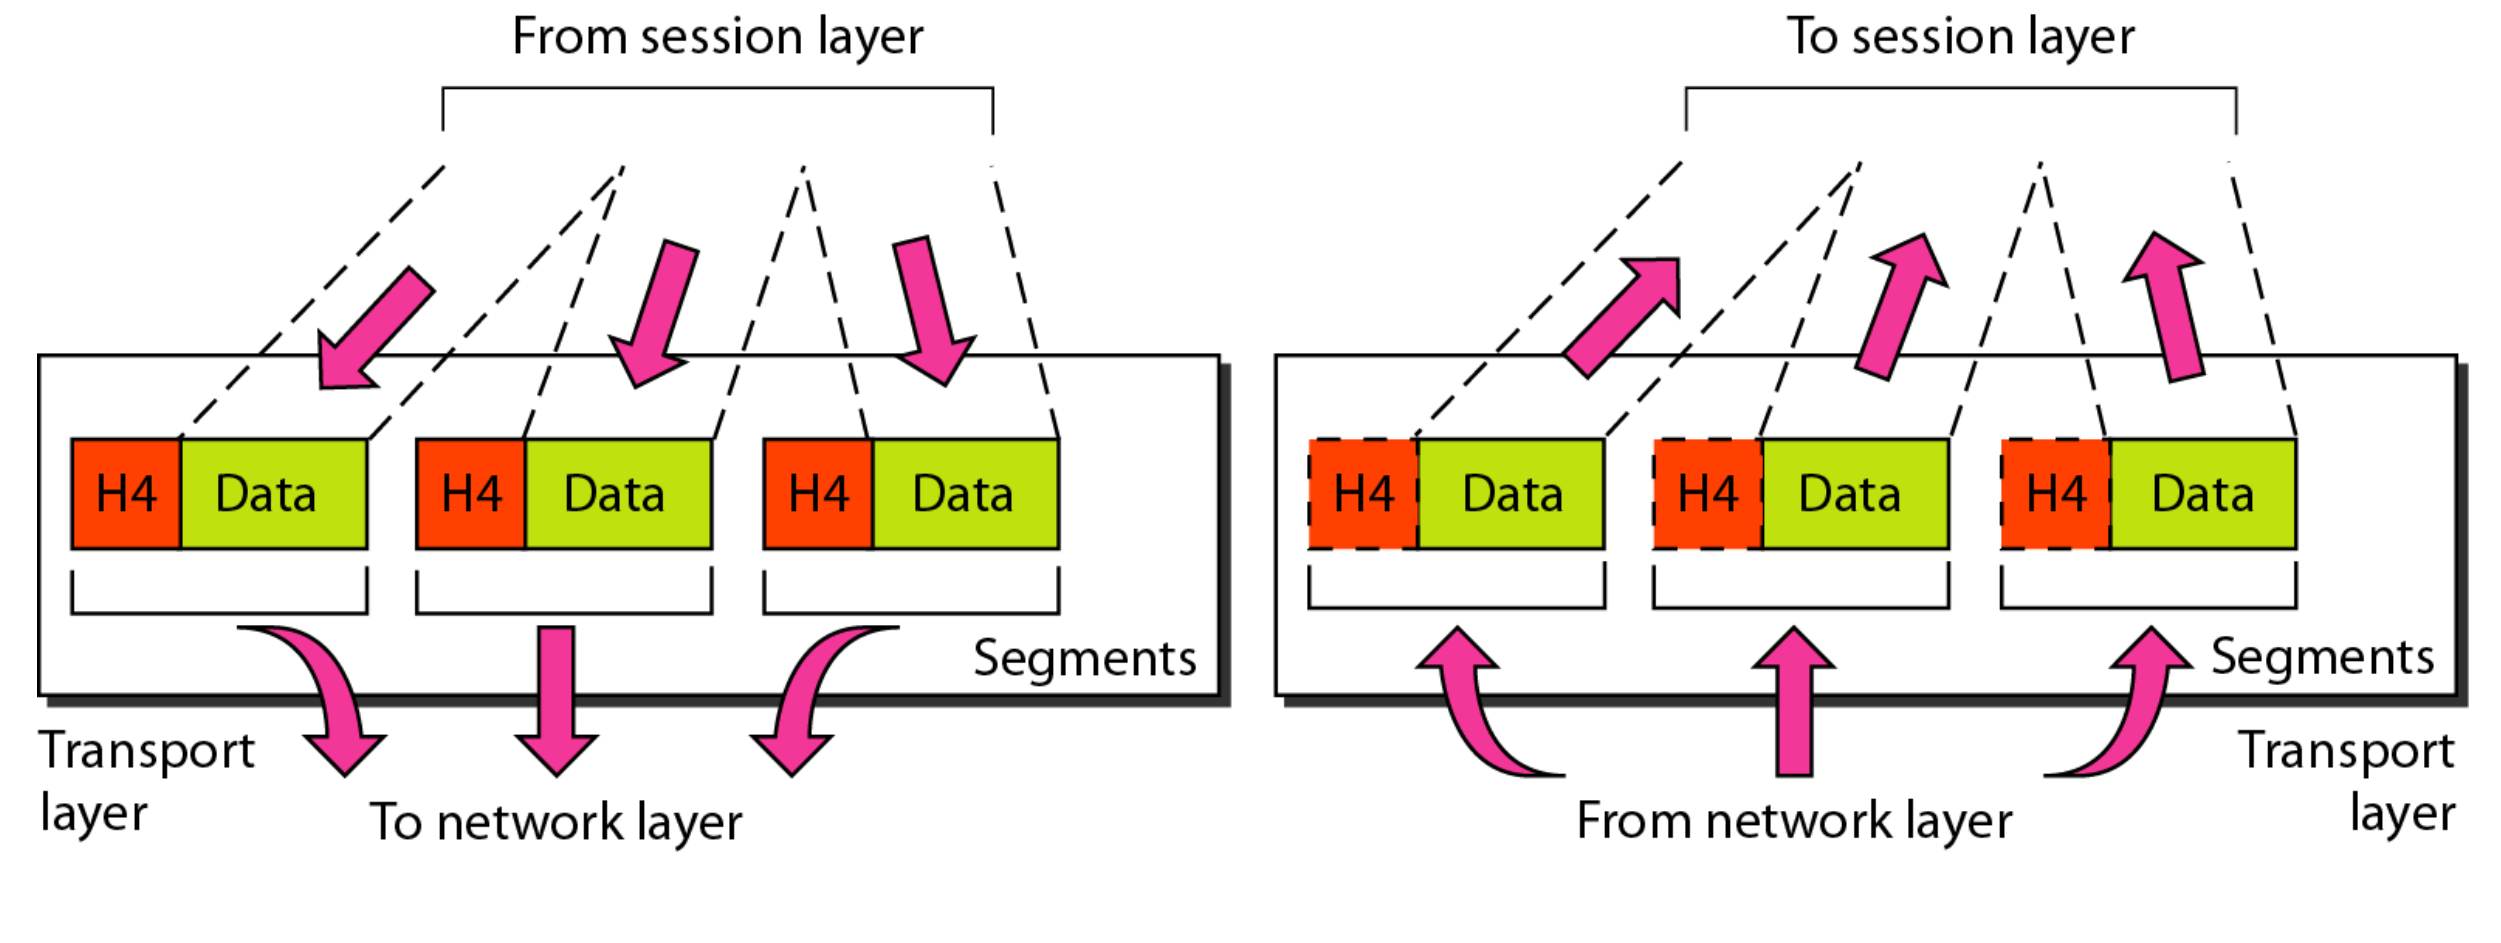
\includegraphics[width=\linewidth]{cap02/osi_trasporto.png}
\end{minipage}\hfill
\begin{minipage}{0.48\linewidth}
È responsabile di \textbf{consegnare un messaggio da un estremo all'altro} e al \textbf{programma
giusto} sull'host di destinazione. Si occupa di:
\begin{itemize}
  \item \textbf{indirizzamento tramite porte}: il livello di rete trova l'\emph{host}, il trasporto
        trova il \emph{processo};
  \item controllo della connessione (con o senza connessione);
  \item \textbf{segmentazione e riassemblaggio} dei messaggi in segmenti;
  \item controllo di flusso e degli errori, da un estremo all'altro.
\end{itemize}
\end{minipage}
\end{figure}

\subsection{5. Livello di sessione (Session)}

\begin{figure}[H]
\centering
\begin{minipage}{0.48\linewidth}\centering
  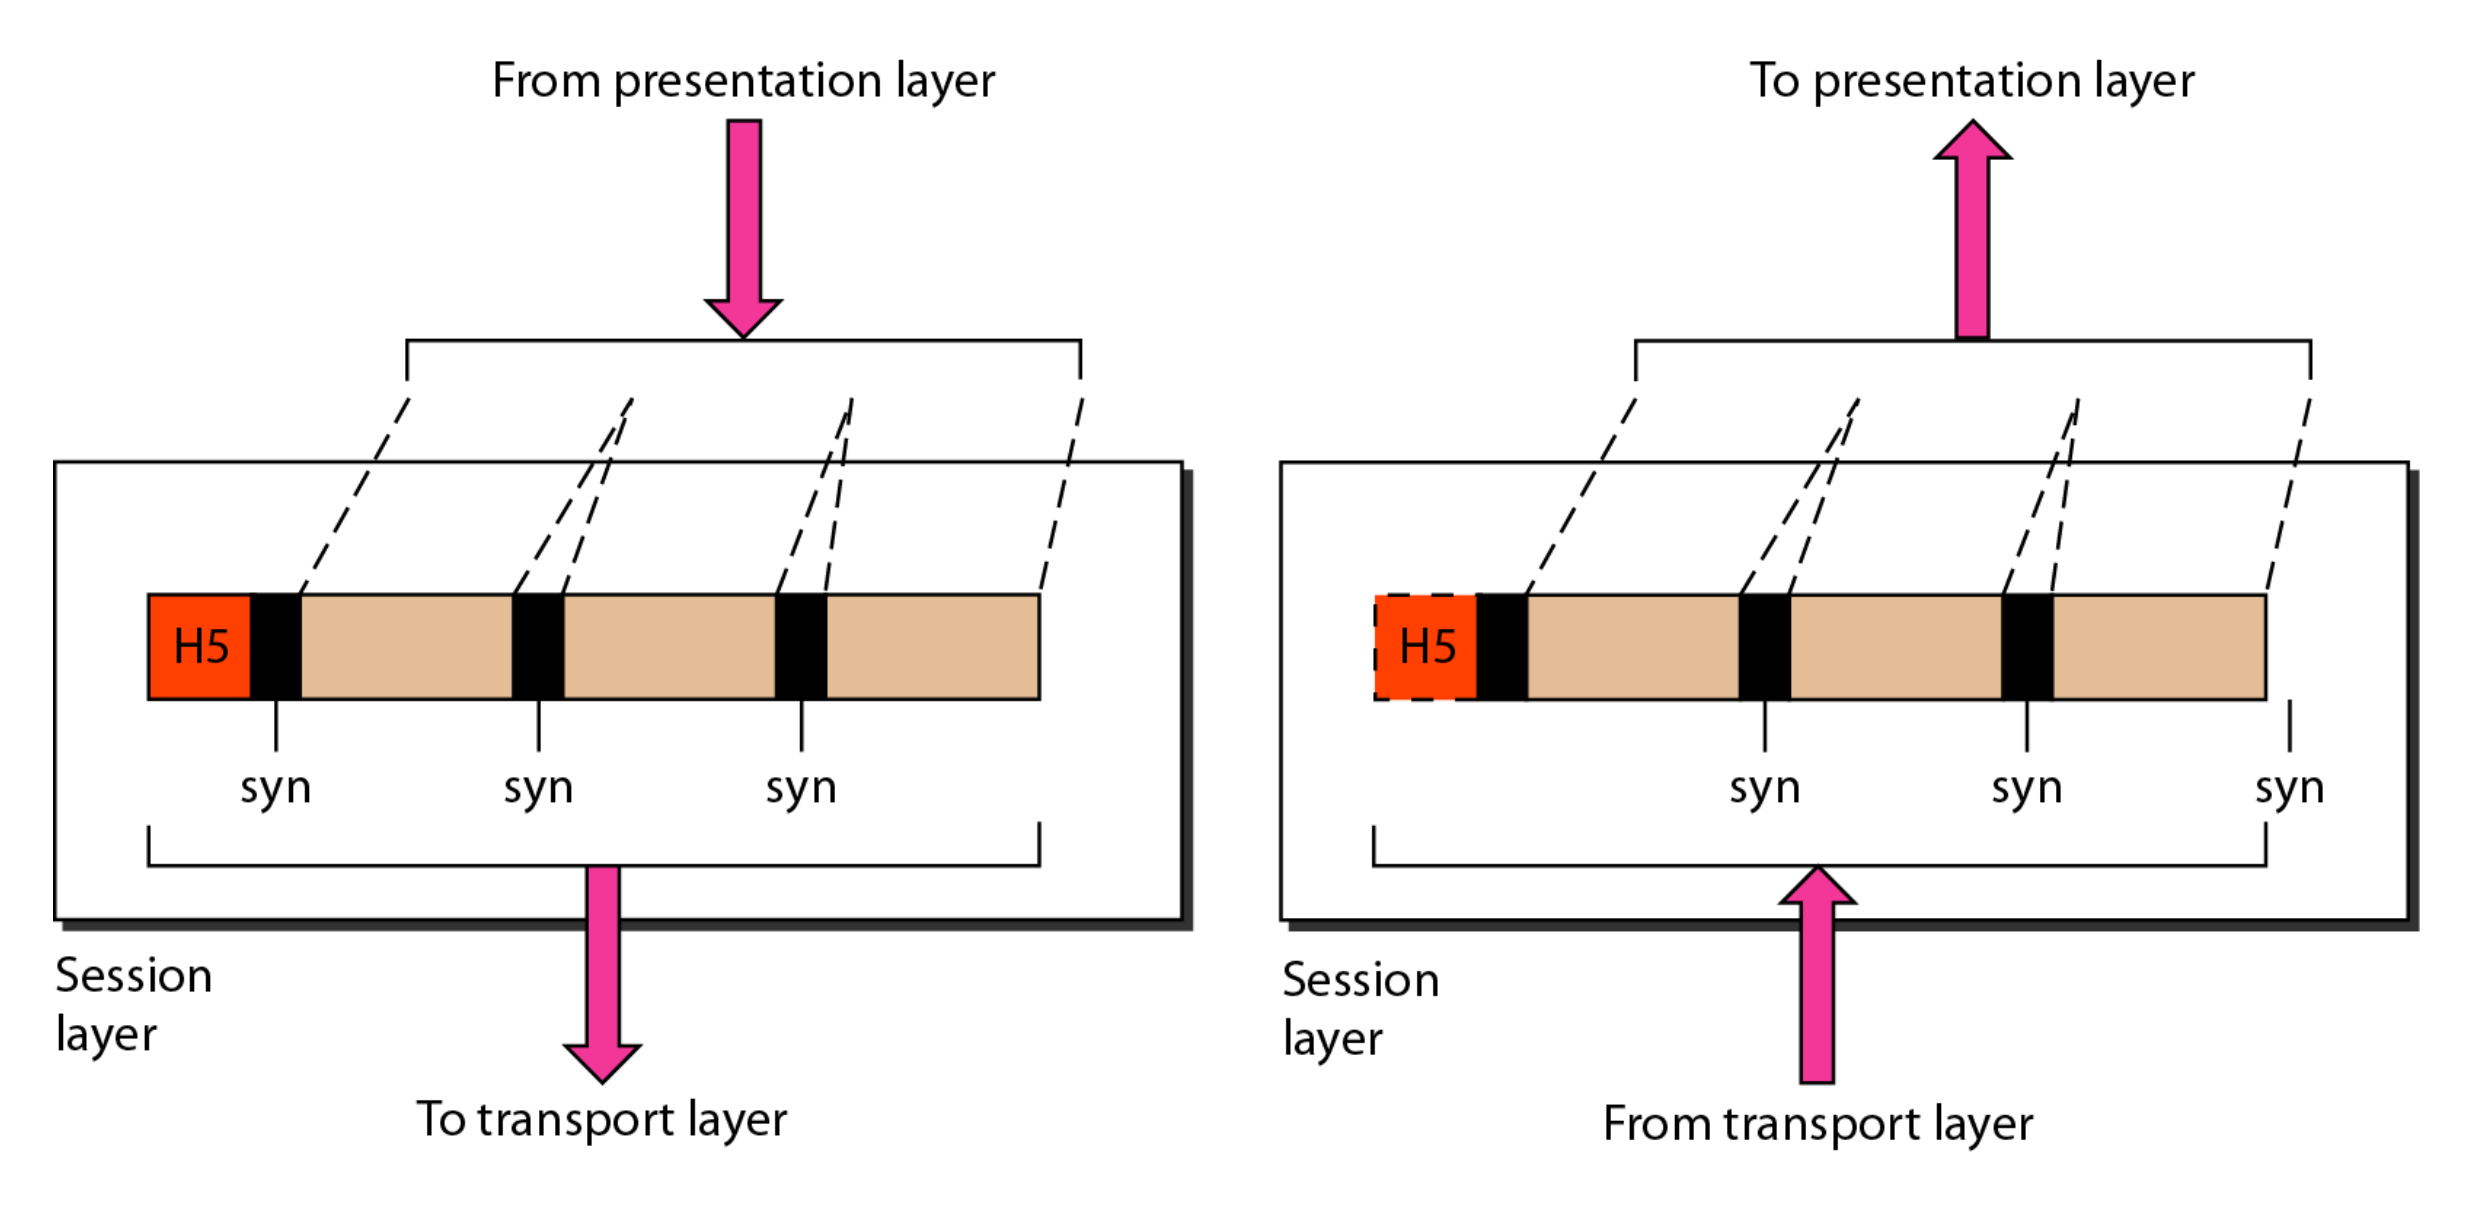
\includegraphics[width=\linewidth]{cap02/osi_sessione.png}
\end{minipage}\hfill
\begin{minipage}{0.48\linewidth}
È responsabile del \textbf{controllo del dialogo}: stabilisce, mantiene e sincronizza l'interazione
tra i due sistemi.
\begin{itemize}
  \item \textbf{chi parla, quando e per quanto};
  \item \textbf{punti di sincronizzazione} (\emph{checkpoint}, i \texttt{syn} della figura): uno scambio
        interrotto riprende dall'ultimo checkpoint invece che dall'inizio.
\end{itemize}
\end{minipage}
\end{figure}

\subsection{6. Livello di presentazione (Presentation)}

\begin{figure}[H]
\centering
\begin{minipage}{0.48\linewidth}\centering
  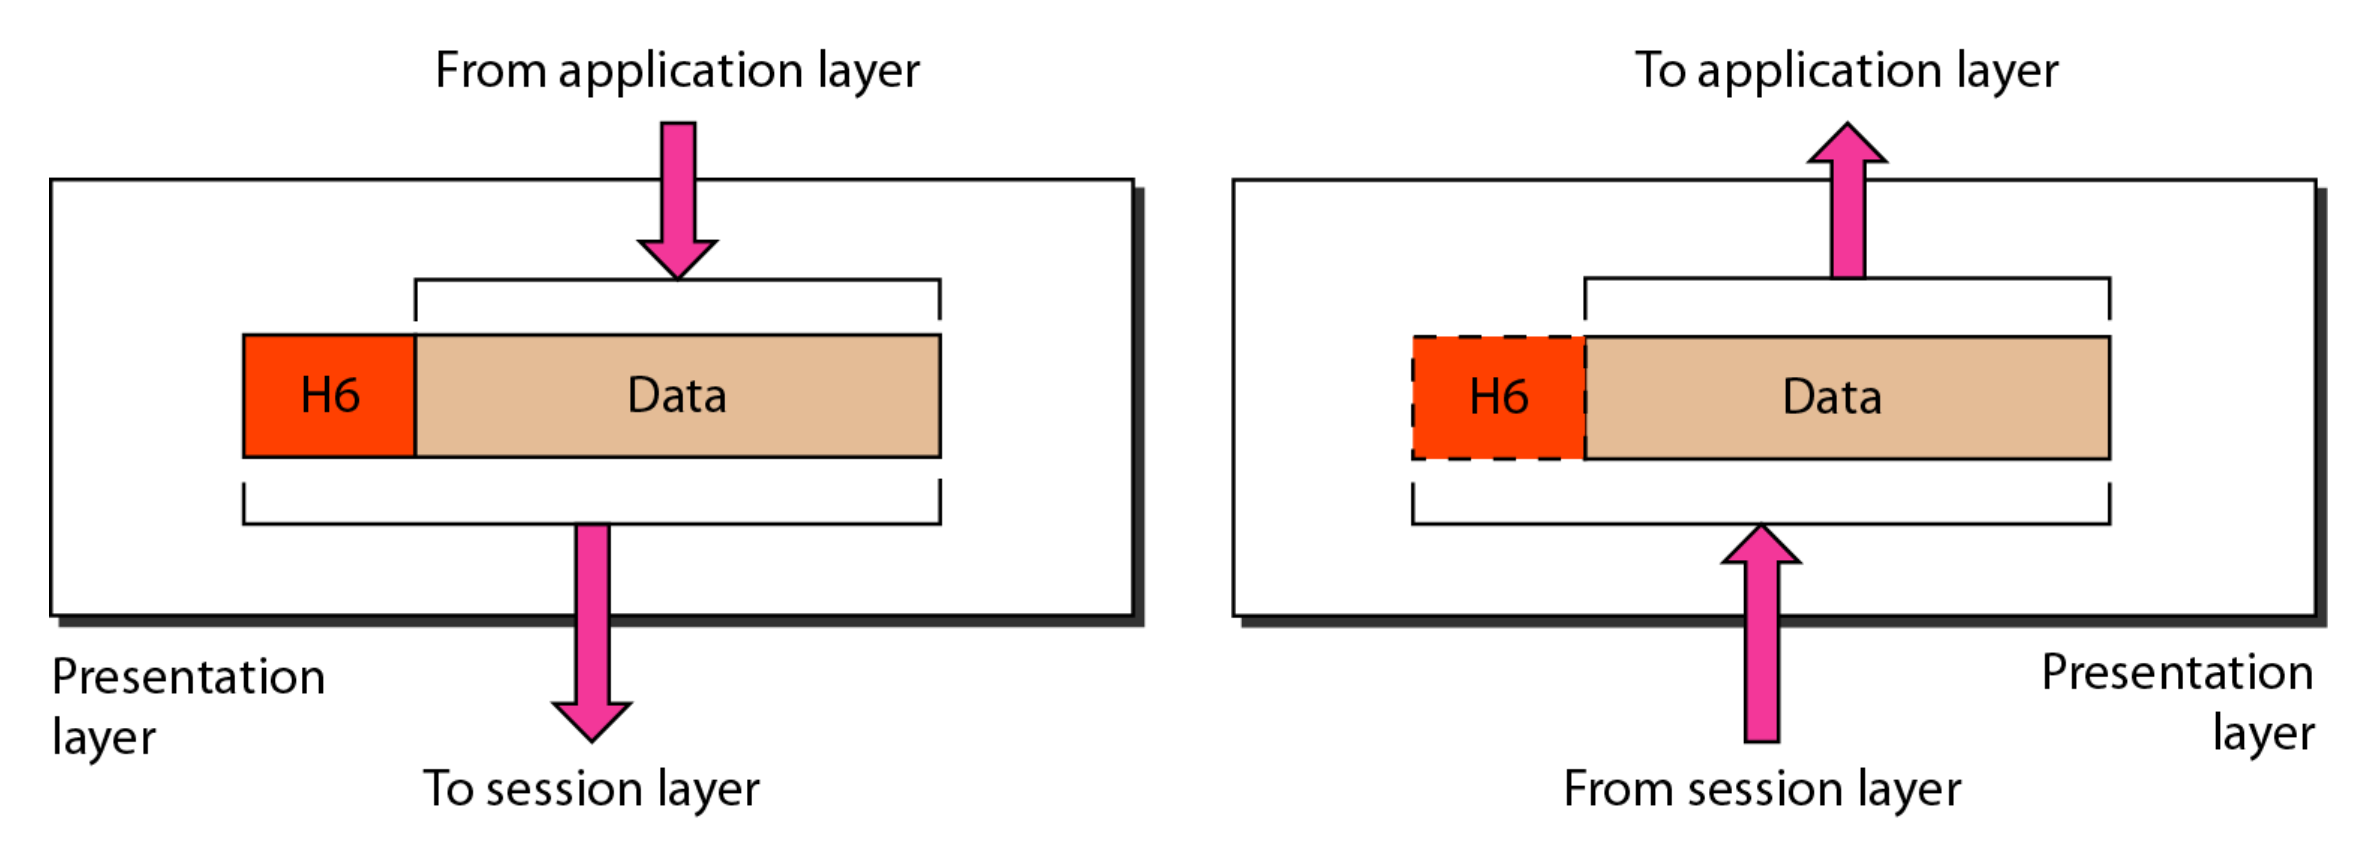
\includegraphics[width=\linewidth]{cap02/osi_presentazione.png}
\end{minipage}\hfill
\begin{minipage}{0.48\linewidth}
È responsabile della \textbf{rappresentazione dei dati}, perché ciò che scrive una parte sia ciò che
legge l'altra:
\begin{itemize}
  \item \textbf{traduzione} tra codifiche diverse (il caso storico è ASCII contro EBCDIC);
  \item \textbf{cifratura} e decifratura;
  \item \textbf{compressione}.
\end{itemize}
\end{minipage}
\end{figure}

\subsection{7. Livello applicativo (Application)}

\begin{figure}[H]
\centering
\begin{minipage}{0.48\linewidth}\centering
  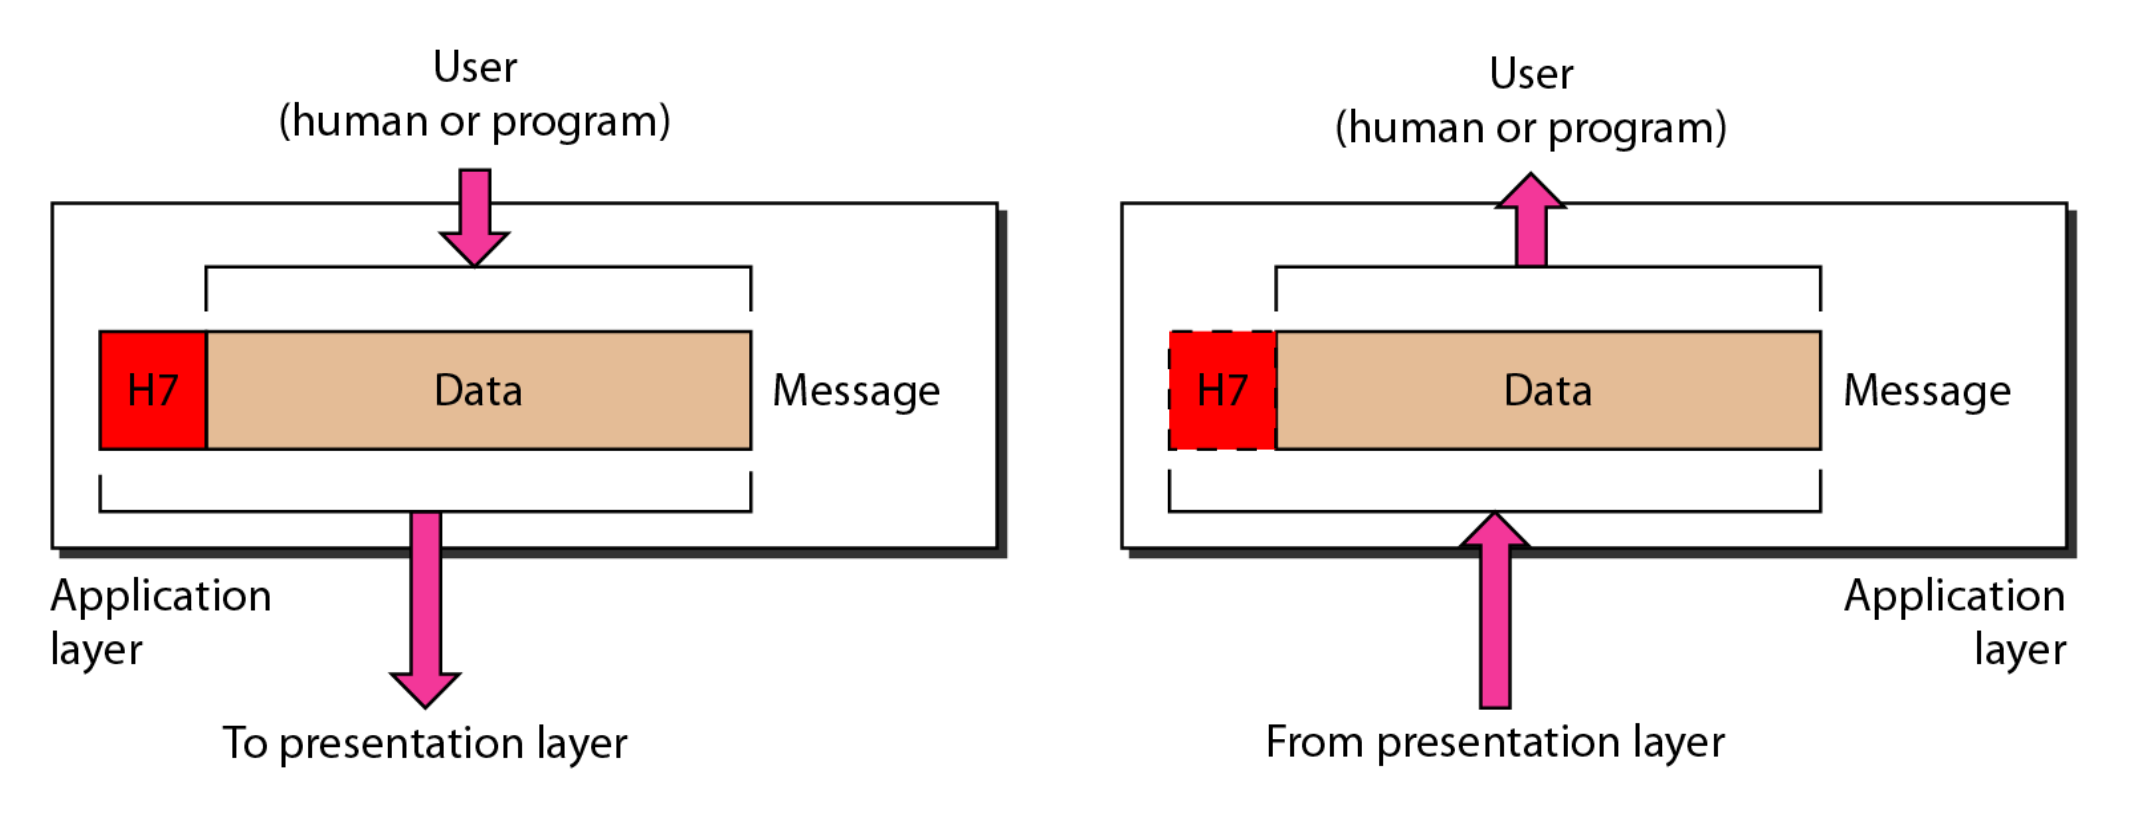
\includegraphics[width=\linewidth]{cap02/osi_applicazione.png}
\end{minipage}\hfill
\begin{minipage}{0.48\linewidth}
È responsabile di \textbf{fornire servizi all'utente} (una persona o un programma), ed è dove vivono i
protocolli che già conoscete per nome:
\begin{itemize}
  \item login remoto (terminale virtuale di rete);
  \item trasferimento e accesso ai file;
  \item posta elettronica;
  \item accesso al World Wide Web.
\end{itemize}
È lo strato che apriremo per primo, perché è quello che si vede.
\end{minipage}
\end{figure}

% ══════════════════════════════════════════════════════════════
\section{Perché OSI non ha vinto}
% ══════════════════════════════════════════════════════════════

Il modello OSI è lo standard \emph{de iure}, ma i suoi protocolli non hanno avuto successo. Le
ragioni sono quattro:

\begin{itemize}
    \item \textbf{Cattivo tempismo} (\emph{bad timing}): quando comparvero i protocolli OSI, TCP/IP era
          già diffuso nelle università di ricerca, e nessun produttore voleva sostenere un secondo stack.
    \item \textbf{Cattiva progettazione} (\emph{bad design}): sia il modello sia i protocolli avevano
          difetti. Sette strati erano un numero ``politico'': sessione e presentazione sono quasi vuoti,
          collegamento e rete sono sovraccarichi.
    \item \textbf{Cattive implementazioni} (\emph{bad implementations}): le prime erano enormi, goffe e
          lente, e la cattiva reputazione è rimasta anche dopo che i prodotti erano migliorati.
    \item \textbf{Cattiva politica} (\emph{bad politics}): era percepito come una creatura dei ministeri
          delle telecomunicazioni europei, della Comunità Europea e poi del governo statunitense,
          mentre TCP/IP arrivava gratis insieme a Berkeley UNIX.
\end{itemize}

Il \textbf{modello} OSI è sopravvissuto ed è ancora il modo in cui si parla di reti; i suoi
\textbf{protocolli} no.

\subsection{L'apocalisse dei due elefanti}

\begin{figure}[H]
    \centering
    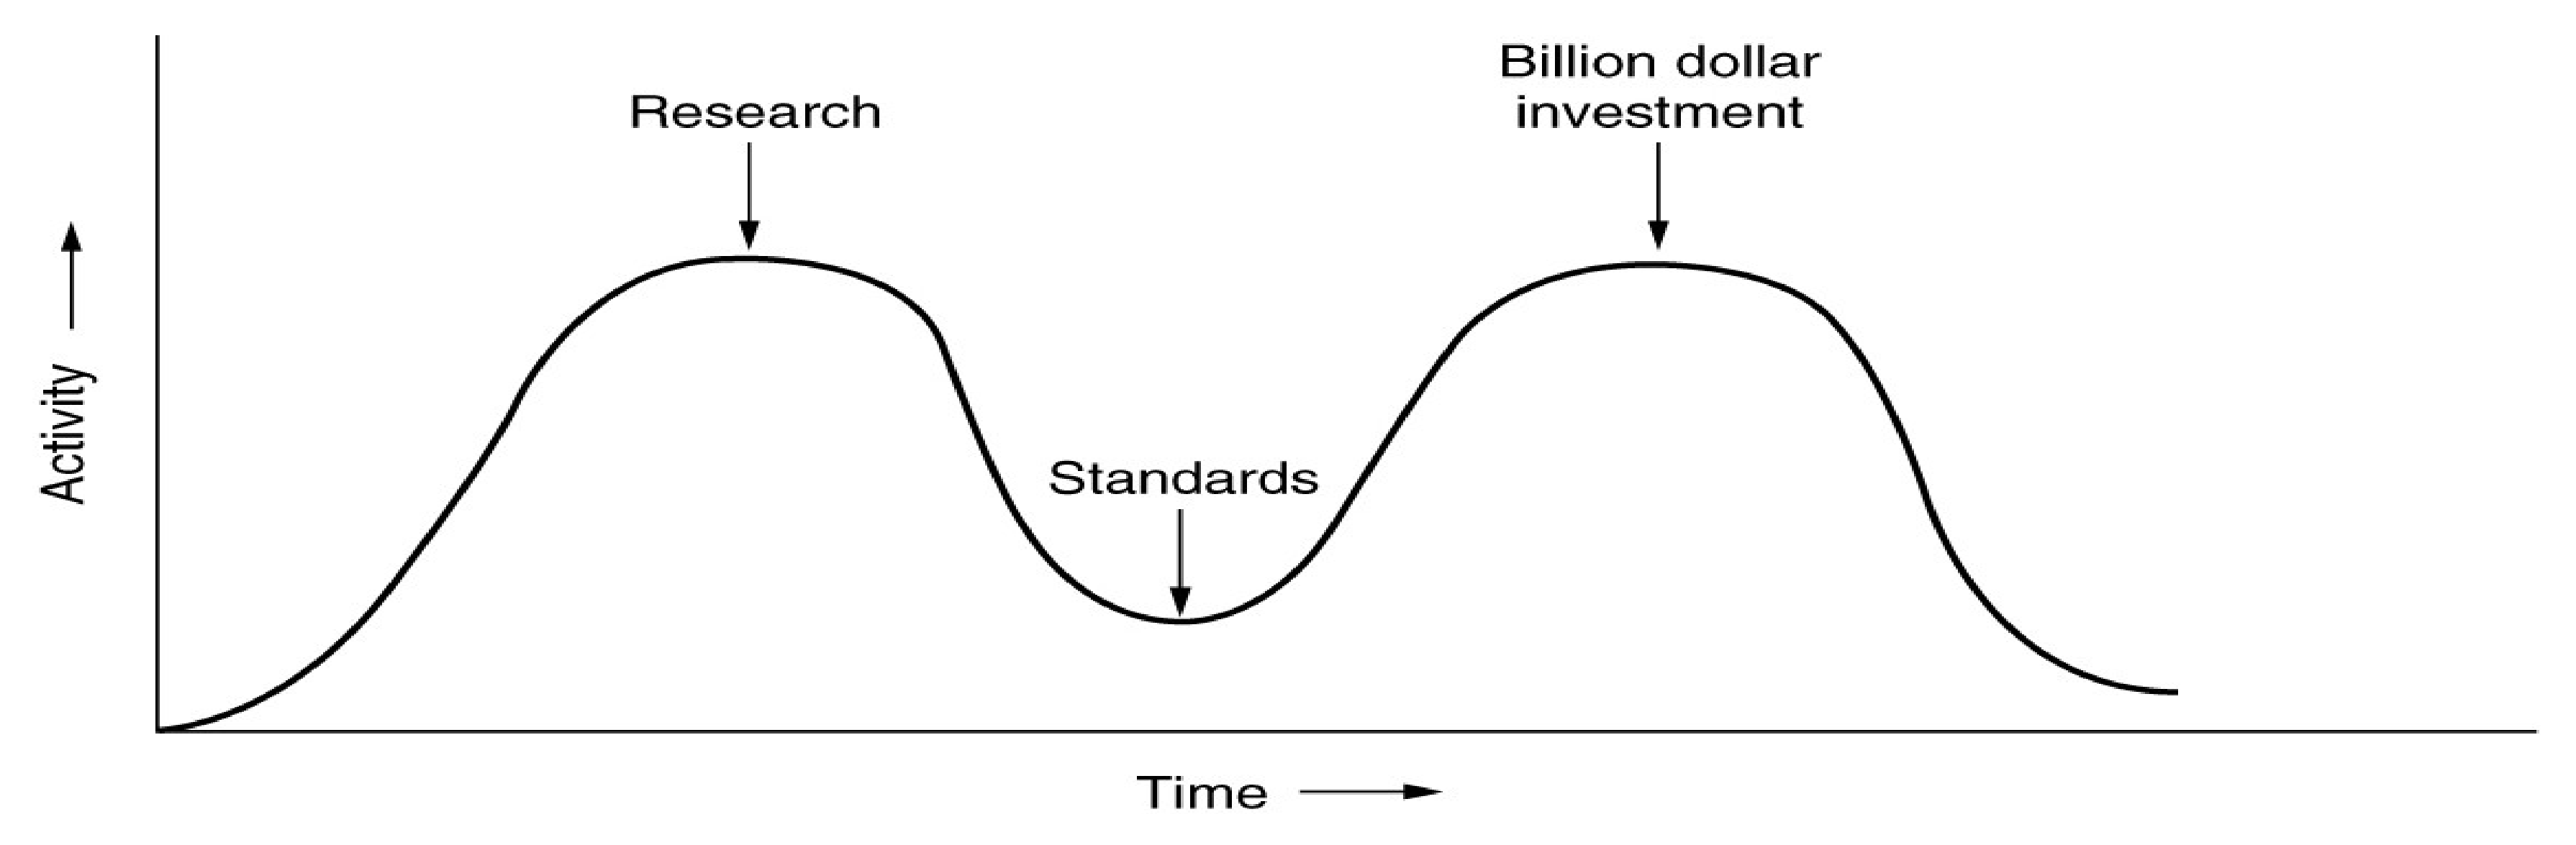
\includegraphics[width=0.5\linewidth]{cap02/due_elefanti.png}
    \caption{L'attività su un argomento: prima la ricerca, poi il miliardo di dollari di investimenti.}
\end{figure}

Quando nasce un nuovo argomento, l'attività ha due ``gobbe'' (i due elefanti): prima un picco di
\textbf{ricerca}, poi, anni dopo, un picco di \textbf{investimenti industriali}. Tra le due c'è una conca.

\begin{itemize}
    \item Uno standard scritto \textbf{troppo presto} congela un argomento che nessuno ha ancora capito.
    \item Uno standard scritto \textbf{troppo tardi} viene ignorato da chi ha già investito in altro.
\end{itemize}

Per evitare il cattivo tempismo, gli standard vanno scritti \textbf{nella conca tra le due gobbe}.
OSI non ci riuscì: arrivò quando TCP/IP aveva già occupato il secondo elefante.

% ══════════════════════════════════════════════════════════════
\section{Cosa non va nel modello TCP/IP}
% ══════════════════════════════════════════════════════════════

Per correttezza, anche il \emph{modello} TCP/IP ha i suoi difetti:

\begin{itemize}
    \item \textbf{non distingue chiaramente} i concetti di servizio, interfaccia e protocollo, cioè
          proprio ciò che OSI aveva fatto bene;
    \item \textbf{non è generale}: non si riesce a usarlo per descrivere altre pile di protocolli
          (provate a descrivere Bluetooth con il modello TCP/IP);
    \item il suo \textbf{livello di collegamento non è un vero strato}, ma un'interfaccia tra l'host e il
          collegamento trasmissivo;
    \item \textbf{non distingue} tra livello fisico e livello di collegamento, che sono due compiti
          completamente diversi.
\end{itemize}

I suoi \textbf{protocolli}, però, erano progettati con cura, ben implementati e distribuiti
\textbf{gratuitamente}.

% ══════════════════════════════════════════════════════════════
\section{De iure e de facto}
% ══════════════════════════════════════════════════════════════

\begin{figure}[H]
\centering
\begin{minipage}{0.45\linewidth}\centering
  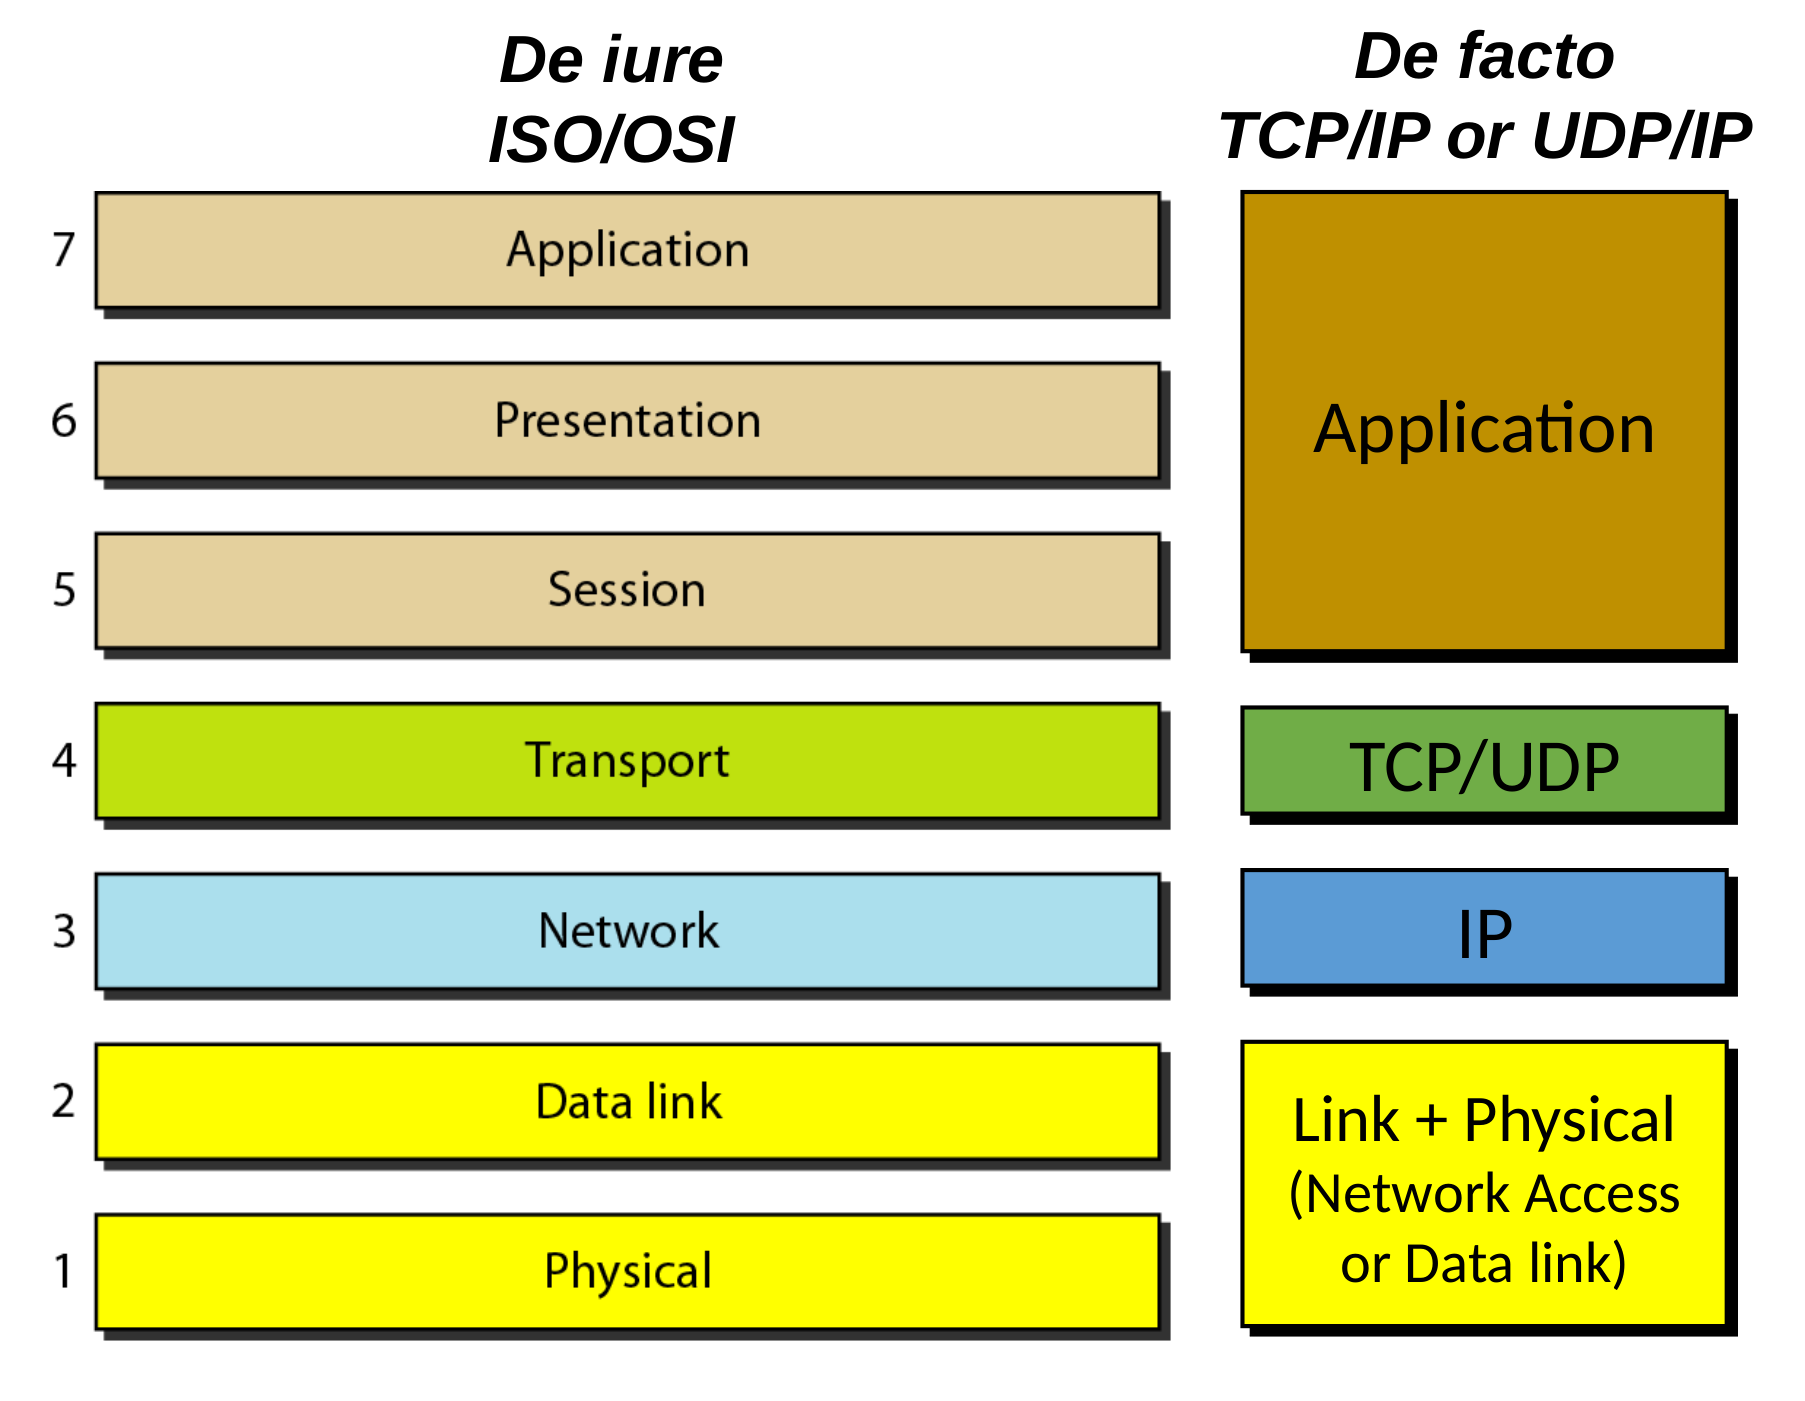
\includegraphics[width=\linewidth]{cap02/de_iure_de_facto.png}
\end{minipage}\hfill
\begin{minipage}{0.5\linewidth}
\begin{itemize}
  \item \textbf{De iure}: ISO/OSI è il modello standard per le reti di calcolatori: completo,
        dettagliato e complesso.
  \item \textbf{De facto}: i protocolli che girano davvero su Internet e sulle reti locali sono
        \textbf{TCP}, \textbf{UDP} e \textbf{IP} (la \emph{Internet Protocol Suite}):
        \begin{itemize}
          \item \textbf{TCP}: \emph{Transmission Control Protocol};
          \item \textbf{UDP}: \emph{User Datagram Protocol};
          \item \textbf{IP}: \emph{Internet Protocol}.
        \end{itemize}
\end{itemize}
In pratica non sono rivali: teniamo il \textbf{modello} per ragionare e i \textbf{protocolli} per lavorare.
\end{minipage}
\caption{Corrispondenza tra la pila ISO/OSI e la pila TCP/IP.}
\end{figure}

\info{IP è il collante}{
    Il protocollo IP è il ``collante'' di tutta la rete di reti che chiamiamo Internet. È l'unico punto
    in cui tutti sono obbligati a mettersi d'accordo: sopra IP ci possono essere TCP o UDP, sotto IP
    Ethernet, Wi-Fi o qualunque altra cosa. È la ``vita stretta'' della clessidra vista nel capitolo 1.
}

% ══════════════════════════════════════════════════════════════
\section{I cinque strati usati nel resto del corso}
% ══════════════════════════════════════════════════════════════

Da qui in avanti il corso conta \textbf{cinque strati}, non sette: è il modello OSI senza sessione e
presentazione, i cui pochi compiti reali vengono svolti direttamente dalle applicazioni. I nomi sono
quelli del Kurose.

\begin{figure}[H]
\centering
\begin{tikzpicture}[every node/.style={font=\small\sffamily}]
  \node[lay app, minimum width=3.4cm, minimum height=0.8cm] (a) at (0,2.4) {Applicazione};
  \node[lay tra, minimum width=3.4cm, minimum height=0.8cm] (t) at (0,1.6) {Trasporto};
  \node[lay net, minimum width=3.4cm, minimum height=0.8cm] (n) at (0,0.8) {Rete};
  \node[lay link, minimum width=3.4cm, minimum height=0.8cm] (l) at (0,0) {Collegamento};
  \node[lay phy, minimum width=3.4cm, minimum height=0.8cm] (p) at (0,-0.8) {Fisico};
  \foreach \n/\osi/\u/\ex in {a/{OSI 7, 6, 5}/messaggio/{HTTP, SMTP, DNS}, t/{OSI 4}/segmento/{TCP, UDP}, n/{OSI 3}/datagramma/{IP}, l/{OSI 2}/frame/{Ethernet, Wi-Fi}, p/{OSI 1}/bit/{rame, fibra, radio}} {
     \node[anchor=east, lbl] at ([xshift=-0.3cm]\n.west) {\osi};
     \node[anchor=west, text=primary!85!black, font=\small\bfseries\sffamily] at ([xshift=0.3cm]\n.east) {\u};
     \node[anchor=west, lbl, text=black!60] at ([xshift=2.4cm]\n.east) {\ex};
  }
  \node[font=\footnotesize\bfseries\sffamily] at (2.7,3.2) {unità di dati};
  \node[font=\footnotesize\bfseries\sffamily] at (4.7,3.2) {esempi};
\end{tikzpicture}
\caption{La pila a cinque strati: corrispondenza con OSI, nome dell'unità di dati ed esempi di protocolli.}
\end{figure}

\begin{table}[H]
\centering
\begin{tabular}{lcl}
\toprule
\textbf{Strato} & \textbf{Corrisponde a OSI} & \textbf{Unità di dati} \\
\midrule
Applicazione & 7, 6 e 5 & messaggio \\
Trasporto & 4 & segmento \\
Rete & 3 & datagramma \\
Collegamento & 2 & frame \\
Fisico & 1 & bit \\
\bottomrule
\end{tabular}
\caption{I cinque strati del corso.}
\end{table}

\warning{Numeri OSI e nomi del corso}{
    I numeri OSI (``livello 3'', ``livello 2'') restano in uso perché li usano tutti nel settore, e li
    useremo anche noi quando serve. Ma la pila che studiamo, dall'alto verso il basso, è quella a
    cinque strati.
}

% ══════════════════════════════════════════════════════════════
\section{La stratificazione oltre Internet}
% ══════════════════════════════════════════════════════════════

Esistono altre pile di protocolli, scelte a seconda del contesto: \textbf{RS-232} per una linea
seriale, \textbf{CAN} all'interno di un veicolo o in automazione industriale. Sono molto più semplici,
e sono comunque stratificate.

\begin{figure}[H]
    \centering
    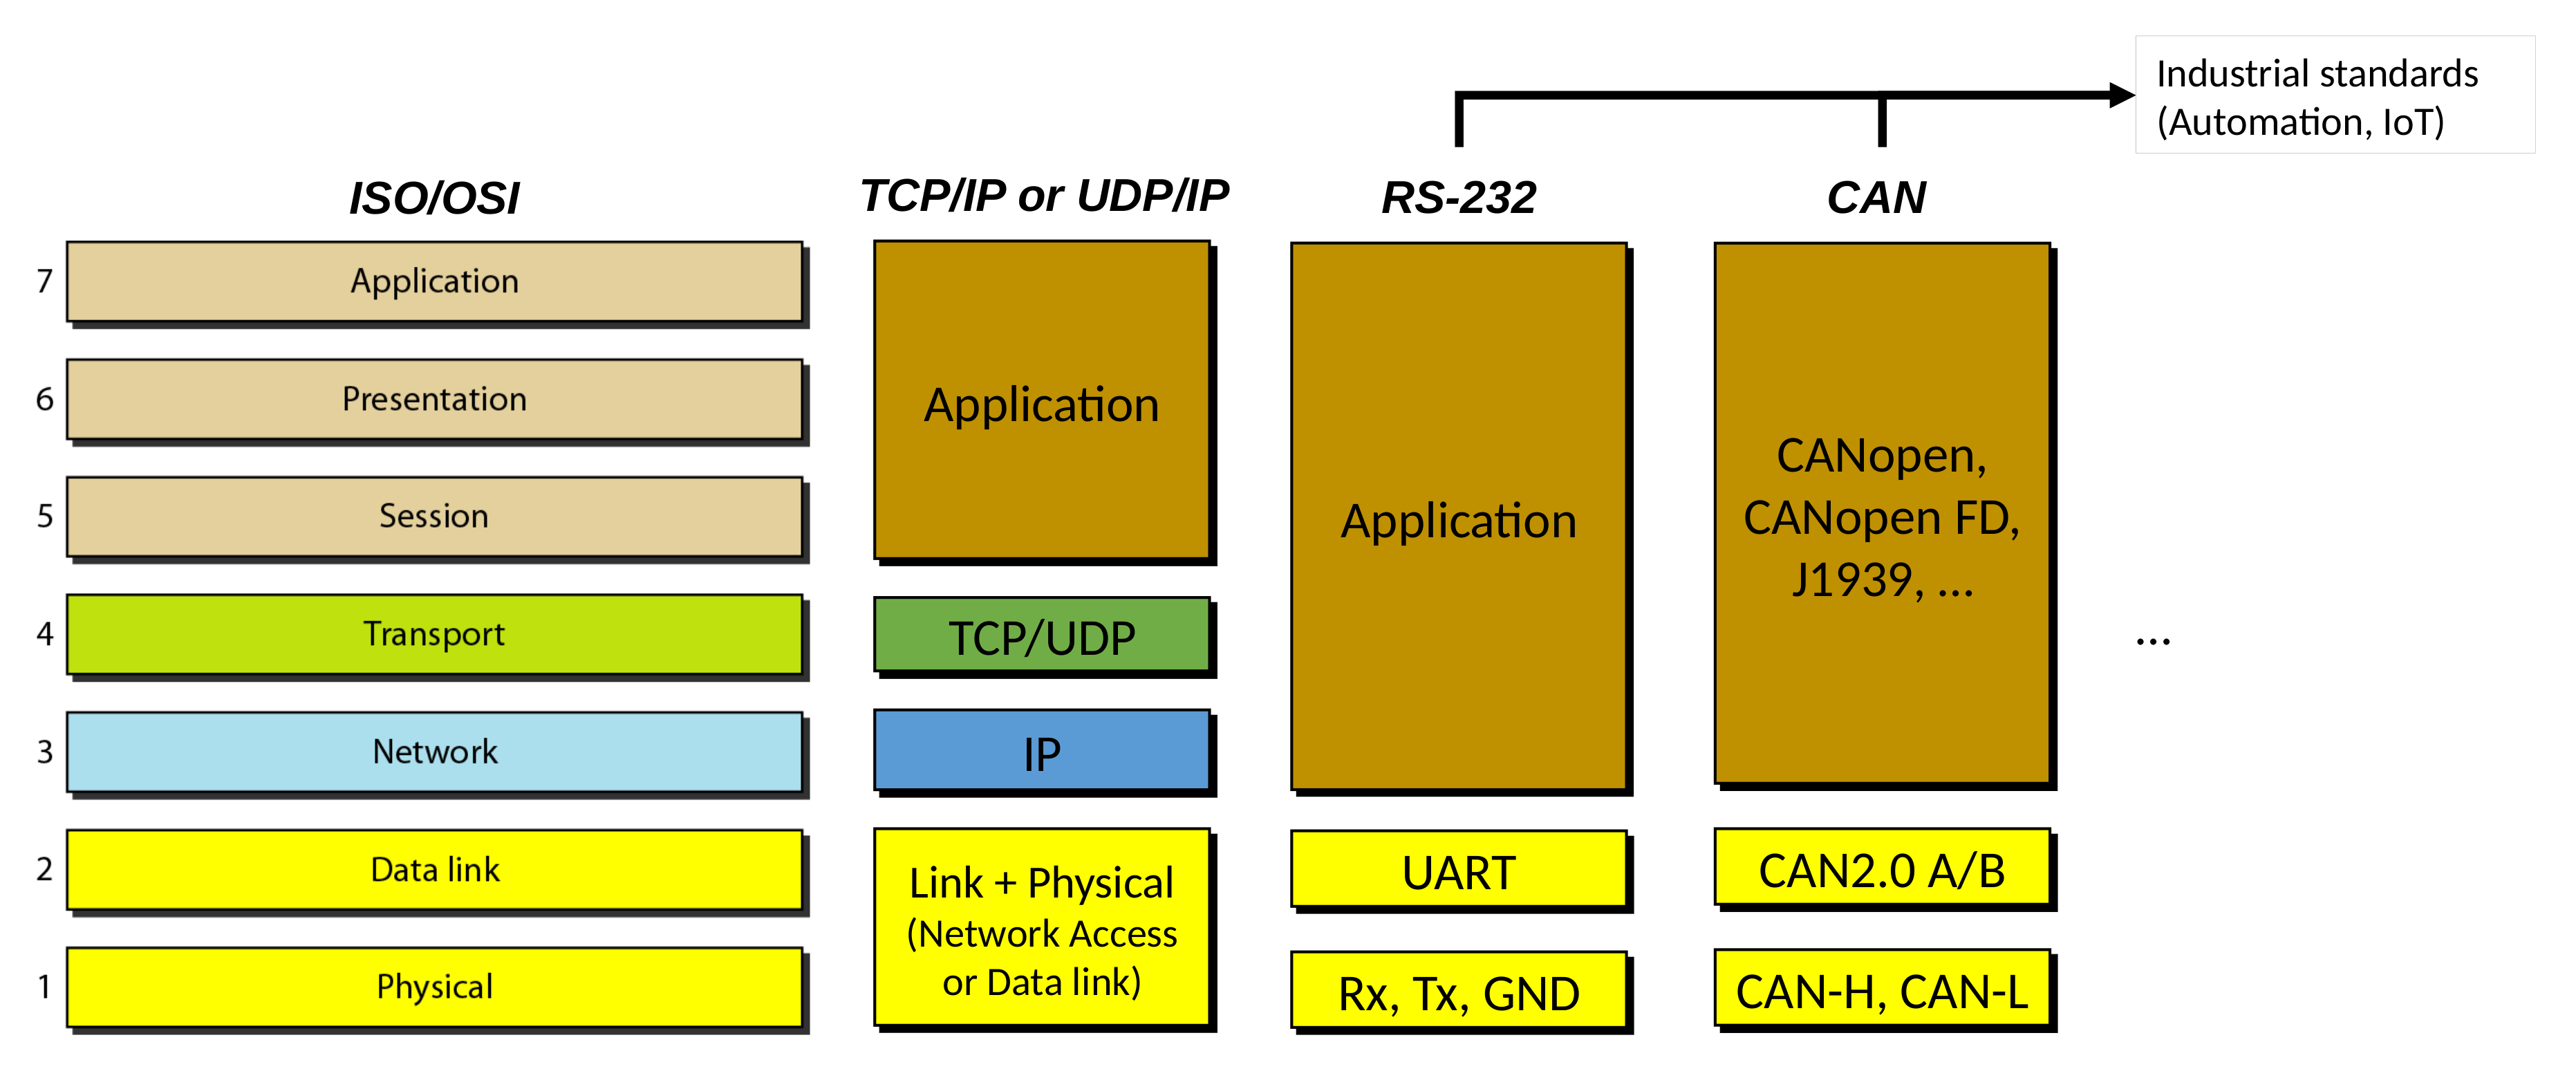
\includegraphics[width=0.75\linewidth]{cap02/altri_modelli.png}
    \caption{Modelli a strati in altri contesti (standard industriali, automazione, IoT).}
\end{figure}

\begin{table}[H]
\centering
\begin{tabular}{cccc}
\toprule
\textbf{Strato OSI} & \textbf{TCP/IP o UDP/IP} & \textbf{RS-232} & \textbf{CAN} \\
\midrule
7--5 & Applicazione & \multirow{3}{*}{Applicazione} & \multirow{3}{*}{\makecell{CANopen, CANopen FD,\\ J1939, \dots}} \\
4 & TCP/UDP & & \\
3 & IP & & \\
\midrule
2 & \multirow{2}{*}{Link + Fisico} & UART & CAN 2.0 A/B \\
1 & & Rx, Tx, GND & CAN-H, CAN-L \\
\bottomrule
\end{tabular}
\caption{In RS-232 e CAN i livelli di collegamento e fisico sono distinti, e tutto il resto è ``applicazione''.}
\end{table}

% ══════════════════════════════════════════════════════════════
\section{Riepilogo}
% ══════════════════════════════════════════════════════════════

\riepilogo{
\begin{itemize}
    \item Una richiesta attraversa troppi pezzi per essere progettata tutta insieme: il sistema si divide
          in \textbf{strati} (\emph{divide et impera}).
    \item Uno strato offre un \textbf{servizio} verso l'alto attraverso un'\textbf{interfaccia}, e usa un
          \textbf{protocollo} in orizzontale con il suo pari. Le due cose sono indipendenti.
    \item La comunicazione tra pari è \textbf{logica}: i dati scendono una pila e risalgono l'altra, e solo
          il livello fisico sposta davvero qualcosa.
    \item I servizi possono essere \textbf{con} o \textbf{senza connessione}, \textbf{affidabili} o no:
          TCP darà un flusso di byte affidabile, UDP un datagram inaffidabile.
    \item L'\textbf{incapsulamento} rende possibile tutto questo: ogni strato tratta ciò che trasporta come
          byte opachi.
    \item OSI ci ha dato sette strati con cui ragionare, TCP/IP i protocolli; nel corso usiamo
          \textbf{cinque strati} con i nomi del Kurose: messaggio, segmento, datagramma, frame, bit.
\end{itemize}
}

Nella prossima parte apriamo la cima della pila, dove stanno le applicazioni.
   % Lezione 02

  % ------------------------------------------------------------------
  \part{Il livello applicativo}
  % ------------------------------------------------------------------
  \chapter{Il livello applicativo: architetture e servizi}

Cominciamo la discesa lungo la pila partendo, come vuole l'approccio top-down, dallo strato più
alto: quello che l'utente vede.

\begin{center}
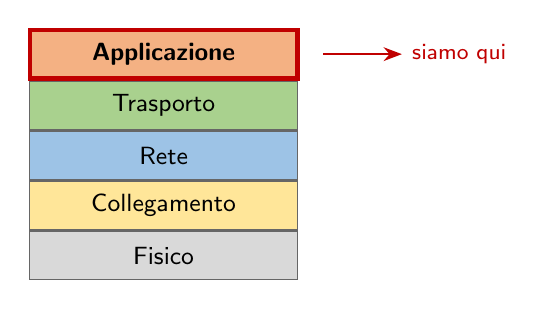
\begin{tikzpicture}[node distance=0pt]
  \node[lay app, minimum width=3.4cm, line width=1.5pt, draw=netred] (a) {\bfseries Applicazione};
  \node[lay tra, minimum width=3.4cm, below=of a] (t) {Trasporto};
  \node[lay net, minimum width=3.4cm, below=of t] (n) {Rete};
  \node[lay link, minimum width=3.4cm, below=of n] (l) {Collegamento};
  \node[lay phy, minimum width=3.4cm, below=of l] (p) {Fisico};
  \draw[-{Stealth}, thick, netred] ([xshift=0.3cm]a.east) -- ++(1,0) node[right, lbl, text=netred] {siamo qui};
\end{tikzpicture}
\end{center}

Abbiamo l'intera pila; ora apriamo lo strato in cima.
\begin{itemize}
    \item Un'applicazione \textbf{non sposta dati}: li consegna allo strato sotto e li ritrova all'altro capo.
    \item Il trasporto le offre (se lo chiede) un \textbf{flusso di dati affidabile}: niente perso, niente fuori ordine.
    \item Due applicazioni su due host si comportano \textbf{come se parlassero direttamente}, purché seguano lo
          stesso protocollo.
\end{itemize}

\info{Che cosa resta da fare al programmatore?}{
    Tutto ciò che sta \textbf{sopra} quel flusso: \textbf{quali messaggi} esistono, \textbf{che cosa significano}
    e \textbf{chi parla per primo}. È esattamente ciò che definisce un protocollo applicativo.
}

% ══════════════════════════════════════════════════════════════
\section{Che cos'è un'applicazione di rete}
% ══════════════════════════════════════════════════════════════

\dfn{Applicazione di rete}{
    Un'\textbf{applicazione di rete} è composta da \textbf{più programmi} che girano su
    \textbf{end system diversi} (host) e che \textbf{comunicano tra loro attraverso la rete}.
}

\begin{esempio}{Un'applicazione Web}
Un'applicazione Web è fatta di due programmi distinti:
\begin{itemize}
    \item il \textbf{browser}, in esecuzione sull'host dell'utente (desktop, laptop, tablet, smartphone);
    \item il \textbf{server Web}, in esecuzione sull'host che ospita il sito.
\end{itemize}
Possono essere scritti in linguaggi diversi e girare su sistemi operativi diversi: l'unica cosa che
devono condividere è il \textbf{protocollo} (HTTP).
\end{esempio}

Qualche applicazione di rete tipica: social network, Web, messaggistica, posta elettronica, giochi
multiutente, streaming video (YouTube, Netflix), condivisione di file P2P, voice over IP,
videoconferenza, ricerca su Internet, login remoto.

\warning{Il Web è tecnicamente un'applicazione}{
    Nel linguaggio comune ``Internet'' e ``Web'' sono usati come sinonimi, ma il Web è
    \textbf{una delle applicazioni} che girano sopra Internet, non è Internet.
}

\subsection{Creare un'applicazione di rete}

\begin{figure}[H]
\centering
\begin{minipage}{0.4\linewidth}\centering
  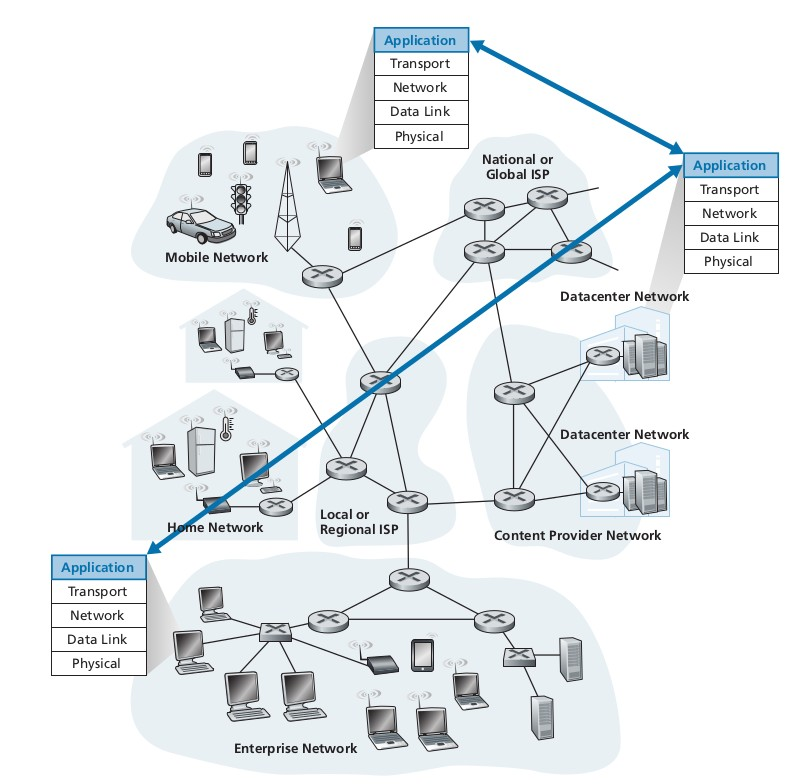
\includegraphics[width=0.9\linewidth]{cap03/app_stack_endsystem.png}
\end{minipage}\hfill
\begin{minipage}{0.56\linewidth}
Creare un'applicazione di rete significa scrivere programmi che:
\begin{itemize}
  \item girano su \textbf{end system diversi}, magari scritti in linguaggi diversi o per sistemi
        operativi diversi;
  \item comunicano attraverso la rete (per esempio tramite \textbf{socket}) usando uno
        specifico \textbf{protocollo}.
\end{itemize}
Notate nella figura che la pila completa (applicazione, trasporto, rete, collegamento, fisico) c'è
\textbf{solo sugli host} ai bordi della rete.
\end{minipage}
\caption{Le applicazioni girano solo sugli end system.}
\end{figure}

\info{Non si scrive software per il nucleo della rete}{
    Non c'è bisogno di scrivere software per i dispositivi del \emph{network core} (router, switch):
    \begin{itemize}
      \item i dispositivi di rete \textbf{non eseguono applicazioni utente};
      \item esistono librerie specifiche (i \textbf{socket}) che implementano le funzionalità di rete.
    \end{itemize}
    È una conseguenza diretta del modello a strati: l'applicazione vede soltanto il servizio che le offre
    il trasporto, e ignora come sia realizzato. Router e switch non eseguono applicazioni utente, e non vi
    lascerebbero installarne una. Questa restrizione \textbf{non è un limite}: è proprio il motivo per cui
    nuove applicazioni nascono e si diffondono così in fretta, senza toccare l'infrastruttura.
}

% ══════════════════════════════════════════════════════════════
\section{Architetture delle applicazioni di rete}
% ══════════════════════════════════════════════════════════════

\dfn{Architettura applicativa}{
    L'\textbf{architettura} di un'applicazione di rete è progettata dallo \textbf{sviluppatore}
    dell'applicazione e determina come l'applicazione è strutturata sui vari end system.
    Le due architetture fondamentali sono \textbf{client-server} e \textbf{peer-to-peer}.
}

\warning{Architettura applicativa e architettura di rete}{
    Non confondete l'\emph{architettura dell'applicazione} (decisa dallo sviluppatore: client-server o P2P)
    con l'\emph{architettura della rete} (la pila a cinque strati di Internet, che è fissata e offre
    all'applicazione un insieme di servizi).
}

\begin{figure}[H]
\centering
\begin{tikzpicture}[every node/.style={font=\footnotesize\sffamily}]
  \begin{scope}
    \node[font=\small\bfseries\sffamily] at (0,2.5) {Client-server};
    \node (srv) at (0,0) {\icon[0.8cm]{server}};
    \node[below=-1pt of srv, text=netred] {server sempre attivo};
    \foreach \a/\ic in {90/laptop, 30/pc, -30/smartphone, -90/laptop, 210/pc, 150/smartphone} {
      \node (c\a) at (\a:2.1) {\icon[0.65cm]{\ic}};
      \draw[msg, netblue, {Stealth}-{Stealth}] (c\a) -- (srv);
    }
    \node[lbl] at (0,-3.1) {i client parlano solo con il server};
  \end{scope}
  \begin{scope}[xshift=8cm]
    \node[font=\small\bfseries\sffamily] at (0,2.5) {Peer-to-peer};
    \foreach \a/\ic [count=\i] in {90/laptop, 30/pc, -30/laptop, -90/pc, 210/laptop, 150/pc} {
      \node (p\i) at (\a:1.9) {\icon[0.65cm]{\ic}};
    }
    \foreach \x/\y in {1/2, 1/4, 2/3, 2/5, 3/6, 4/5, 5/6, 6/1, 3/4} \draw[msg, netgreen, {Stealth}-{Stealth}] (p\x) -- (p\y);
    \node[lbl] at (0,-3.1) {i peer comunicano direttamente tra loro};
  \end{scope}
\end{tikzpicture}
\caption{Le due architetture applicative fondamentali.}
\end{figure}

\subsection{Architettura client-server}

\dfn{Architettura client-server}{
    I nodi sono \textbf{eterogenei}: esiste un host \textbf{sempre attivo} (il \emph{server}) che fornisce
    servizi in risposta alle richieste di molti altri host (i \emph{client}).
}

\begin{itemize}
    \item I client \textbf{non comunicano direttamente} tra loro: due browser non si scambiano mai nulla.
    \item Il server ha un \textbf{indirizzo fisso e ben noto} (un nome o un indirizzo IP): un client può
          sempre contattarlo inviandogli un pacchetto di richiesta.
    \item \textbf{Il client parla per primo}: il server aspetta di essere contattato, e risponde.
    \item Spesso servono \textbf{molti server} per reggere tutte le richieste; il client di solito non se
          ne accorge e li percepisce come un server unico.
\end{itemize}

I server multipli possono essere organizzati in tre modi:

\begin{itemize}
    \item \textbf{raggruppati in data center}, con un numero enorme di server in un unico luogo: vanno
          alimentati, raffreddati, mantenuti e ben collegati;
    \item \textbf{sparsi come server distribuiti} in tutto il mondo: vanno interconnessi e coordinati;
    \item organizzati in \textbf{data center distribuiti}, combinando le due soluzioni: è ciò che fanno davvero
          i grandi fornitori.
\end{itemize}

E il fornitore continua a pagare, mese dopo mese, l'interconnessione e la banda che esce da quegli edifici.

\warning{La conseguenza del client-server}{
    Tutto ciò che l'applicazione fa passa per il server, che è quindi insieme il \textbf{limite alla
    scalabilità} (quanti client si possono servire) e il \textbf{punto di guasto unico} (\emph{single point of
    failure}): se il server cade, il servizio non esiste più per nessuno.
}

\begin{esempio}{Il Web come applicazione client-server}
C'è un server Web sempre attivo che riceve richieste dai browser degli utenti. Quando riceve la
richiesta di un oggetto (una pagina, un'immagine), risponde inviando l'oggetto richiesto. Il server
è raggiungibile da tutti gli host, perché il suo indirizzo è noto, ed è acceso quando lo si interroga.
Richiesta, risposta, e un server che c'era già prima che qualcuno chiedesse: è tutta qui la forma del
client-server.
\end{esempio}

\subsection{Architettura peer-to-peer (P2P)}

\dfn{Architettura peer-to-peer}{
    I nodi sono (idealmente) \textbf{omogenei}: l'applicazione sfrutta la \textbf{comunicazione diretta}
    tra coppie di host collegati in modo \textbf{intermittente}, detti \emph{peer}. I peer non sono di
    proprietà del fornitore del servizio, ma sono computer controllati dagli utenti.
}

\begin{itemize}
    \item È usata spesso per applicazioni ad \textbf{alta intensità di traffico} (condivisione di file).
    \item Non c'è un server unico con indirizzo fisso: ogni peer ha il proprio indirizzo, che può anche cambiare.
    \item È \textbf{auto-scalabile} (\emph{self-scalability}): ogni peer genera carico chiedendo un file, ma
          aggiunge anche \textbf{capacità} servendolo ad altri. La capacità cresce insieme alla domanda: nessun
          progetto client-server ha questa proprietà.
    \item È \textbf{economica}: non servono infrastrutture né grande banda da parte del fornitore.
    \item Ha però problemi di \textbf{sicurezza}, \textbf{prestazioni} e \textbf{affidabilità}: nessuno possiede
          le macchine coinvolte.
\end{itemize}

\info{Il P2P puro è raro: le architetture ibride}{
    Le applicazioni P2P pure sono rare: la maggior parte ha un'architettura \textbf{ibrida}. In molte
    applicazioni di messaggistica e di telefonia su Internet un \textbf{server} tiene traccia degli
    indirizzi IP degli utenti, ma i messaggi da utente a utente viaggiano \textbf{direttamente} tra gli
    host, senza passare per server intermedi. Nella condivisione di file il server può anche tenere
    l'elenco dei file disponibili, per velocizzare la ricerca (così facevano Napster e, in parte,
    BitTorrent con i tracker).
}

\begin{figure}[H]
\centering
\begin{tikzpicture}[every node/.style={font=\footnotesize\sffamily}]
  \node (S) at (0,2.2) {\icon[0.7cm]{server}};
  \node[right=2pt of S, lbl, text width=3.2cm, align=left] {server di indicizzazione: ``Bob è all'indirizzo X''};
  \node (A) at (-3.5,0) {\icon[1cm]{laptop}}; \node[below=-2pt of A] {Alice};
  \node (B) at (3.5,0) {\icon[0.9cm]{pc}}; \node[below=-2pt of B] {Bob};
  \draw[msg, dashed, netblue] (A) -- node[above, sloped] {1. dov'è Bob?} (S);
  \draw[msg, dashed, netblue] (B) -- node[above, sloped] {0. registrazione} (S);
  \draw[msg, very thick, netgreen, {Stealth}-{Stealth}] (A) -- node[below=2pt] {2. messaggi diretti, peer-to-peer} (B);
\end{tikzpicture}
\caption{Un'architettura ibrida: il server serve solo a trovarsi, poi i peer parlano direttamente.}
\end{figure}

% ══════════════════════════════════════════════════════════════
\section{Comunicazione tra processi}
% ══════════════════════════════════════════════════════════════

Come abbiamo già detto, chi comunica \textbf{non è un programma e non è una macchina}, ma un
\textbf{processo}: un programma in esecuzione, su macchine diverse e potenzialmente con sistemi operativi diversi.

\begin{itemize}
    \item Nel Web il processo del browser scambia messaggi con il processo del server Web.
    \item Nella condivisione di file P2P un file passa dal processo di un peer al processo di un altro peer.
\end{itemize}

\dfn{Processo client e processo server}{
    In ogni coppia di processi che comunicano:
    \begin{itemize}
      \item il \textbf{processo client} è quello che \textbf{inizia} la comunicazione;
      \item il \textbf{processo server} è quello che \textbf{attende} di essere contattato.
    \end{itemize}
}

Nel Web il browser è il client e il server Web è il server. Nel P2P il peer che scarica fa da
client e quello che carica fa da server: in un'applicazione P2P i processi possono
\textbf{cambiare ruolo}, e lo stesso peer può essere client su una connessione e server su un'altra.

\subsection{I socket}

La maggior parte delle applicazioni è fatta di coppie di processi che si mandano messaggi
attraverso la rete sottostante. Il punto in cui un processo ``consegna'' i messaggi alla rete ha un
nome preciso.

\dfn{Socket}{
    Seguendo il modello a strati, un \textbf{socket} è l'\textbf{interfaccia software tra il livello
    applicativo e il livello di trasporto}: è la ``porta'' attraverso cui un processo invia e riceve
    messaggi sulla rete. È anche l'\textbf{API} (\emph{Application Programming Interface}) tra
    l'applicazione e la rete.
}

\begin{figure}[H]
    \centering
    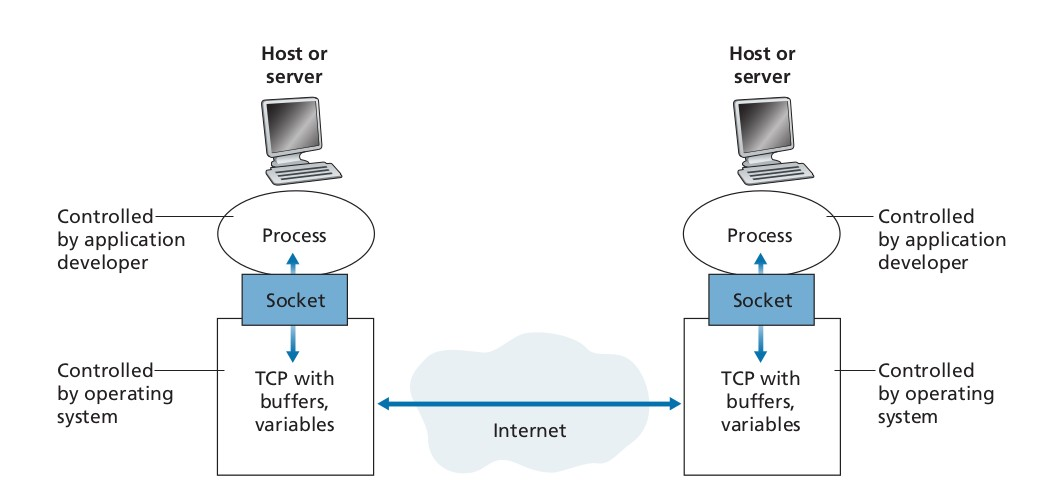
\includegraphics[width=0.72\linewidth]{cap03/processi_socket.png}
    \caption{Il processo è controllato dallo sviluppatore; ciò che sta sotto il socket (TCP con i suoi buffer e le sue variabili) è controllato dal sistema operativo.}
\end{figure}

\begin{esempio}{I socket come cassette postali}
\begin{center}
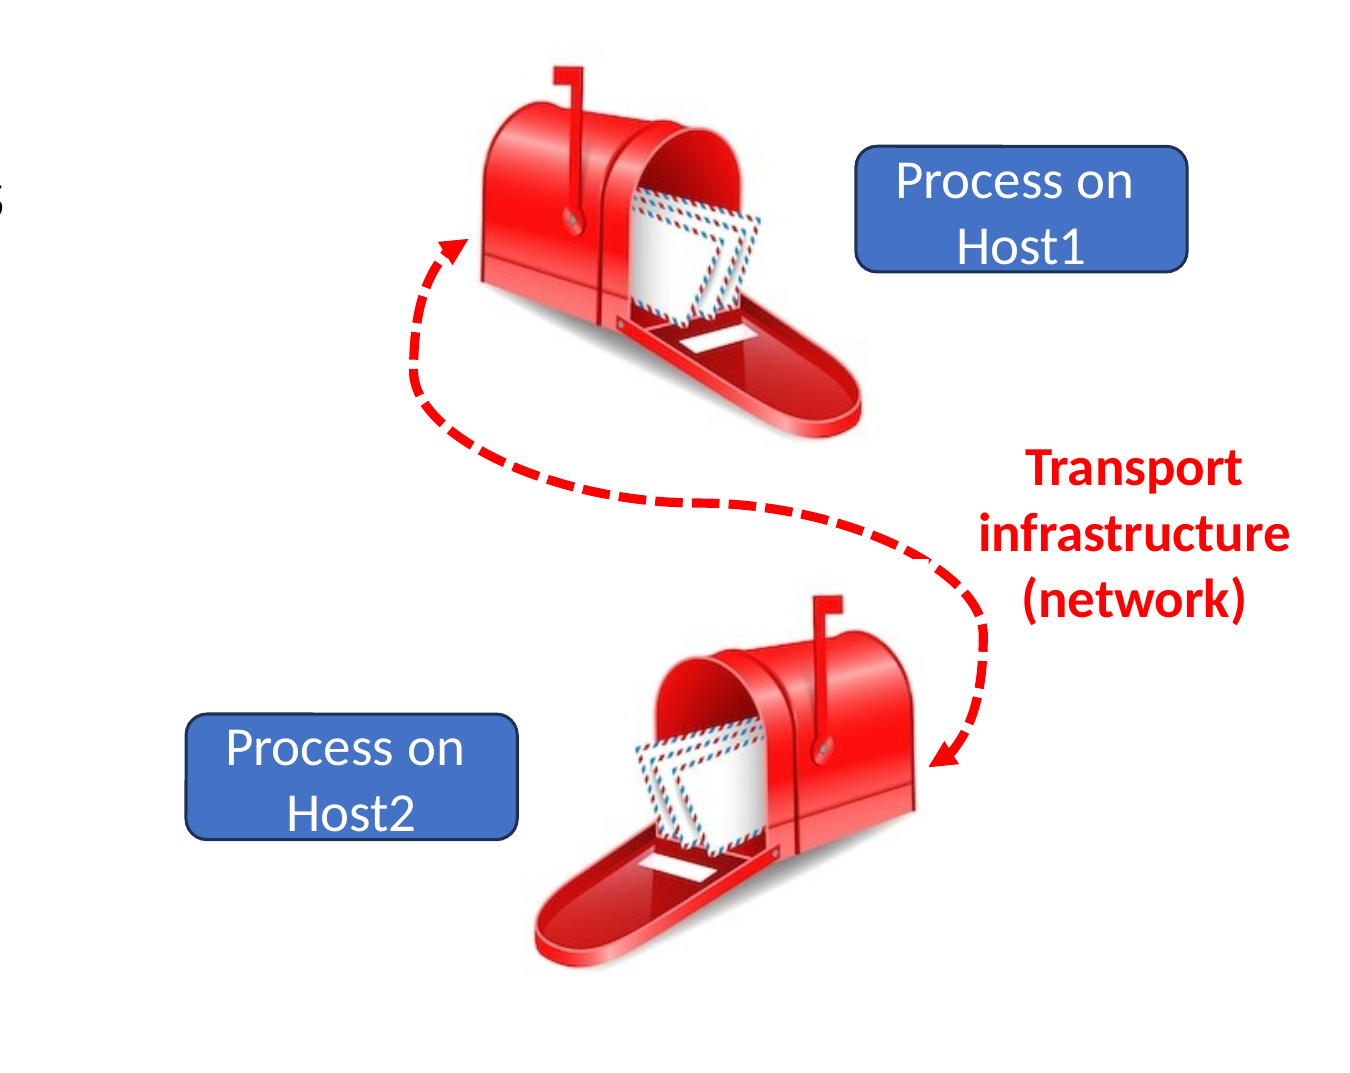
\includegraphics[width=0.42\linewidth]{cap03/socket_cassetta.png}
\end{center}
\begin{itemize}
    \item Un processo che vuole mandare un messaggio a un processo su un altro host \textbf{lo mette nella
          cassetta postale} (il socket).
    \item Il processo mittente dà per scontato che, dall'altra parte della sua porta, ci sia
          un'\textbf{infrastruttura di trasporto} che porterà il messaggio fino alla cassetta del destinatario.
    \item Quando il messaggio arriva all'host di destinazione, passa attraverso la cassetta (il socket) del
          processo ricevente.
\end{itemize}
Chi imbuca una lettera non deve sapere come funziona il sistema postale.
\end{esempio}

\begin{figure}[H]
\centering
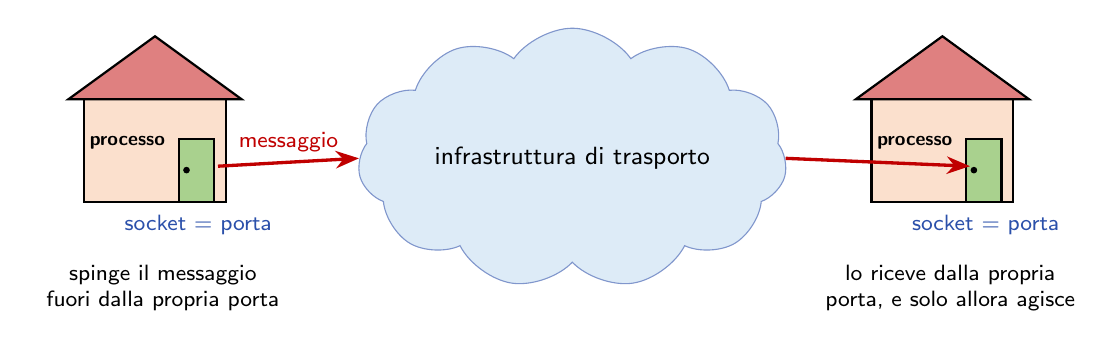
\begin{tikzpicture}[every node/.style={font=\footnotesize\sffamily}]
  \newcommand{\casa}[2]{%
    \begin{scope}[shift={(#1)}]
      \draw[thick, fill=lapp!40] (0,0) rectangle (1.8,1.3);
      \draw[thick, fill=netred!50] (-0.2,1.3) -- (0.9,2.1) -- (2.0,1.3) -- cycle;
      \draw[thick, fill=ltra] (1.2,0) rectangle (1.65,0.8);
      \fill (1.3,0.4) circle (1.2pt);
      \node[font=\scriptsize\bfseries\sffamily] at (0.55,0.75) {#2};
    \end{scope}}
  \casa{0,0}{processo}
  \casa{10,0}{processo}
  \node[text=netblue] at (1.45,-0.3) {socket = porta};
  \node[text=netblue] at (11.45,-0.3) {socket = porta};
  \node[netcloud, minimum width=4.5cm, minimum height=1.6cm] (net) at (6.2,0.55) {infrastruttura di trasporto};
  \draw[-{Stealth}, very thick, netred] (1.7,0.45) -- node[above, lbl] {messaggio} (net.west);
  \draw[-{Stealth}, very thick, netred] (net.east) -- (11.25,0.45);
  \node[lbl, text width=3.2cm] at (1,-1.1) {spinge il messaggio fuori dalla propria porta};
  \node[lbl, text width=3.2cm] at (11,-1.1) {lo riceve dalla propria porta, e solo allora agisce};
\end{tikzpicture}
\caption{Un processo è una casa e il suo socket è la porta: il mittente spinge fuori il messaggio e dà per scontato che qualcosa, fuori, lo porti a destinazione.}
\end{figure}

\warning{Cosa controlla lo sviluppatore}{
    Lo sviluppatore ha il \textbf{controllo completo} di tutto ciò che sta sul lato applicativo del
    socket, ma \textbf{pochissimo controllo} sul lato del trasporto. Può soltanto:
    \begin{enumerate}
      \item \textbf{scegliere il protocollo di trasporto} (TCP o UDP);
      \item eventualmente impostare qualche parametro del trasporto (dimensione massima dei buffer, dei
            segmenti, \dots).
    \end{enumerate}
    Scelto il protocollo, l'applicazione viene costruita dando per scontati i servizi che quel protocollo offre.
    La scelta si fa \textbf{una volta, all'inizio}, e tutto il resto ne discende: è una \textbf{decisione di
    progetto}, non un dettaglio di configurazione.
}

\subsection{Indirizzare i processi: indirizzo e identificatore}

Riprendendo l'analogia postale, un processo ha bisogno di un \textbf{indirizzo} per ricevere
messaggi. Ma su un host girano contemporaneamente molte applicazioni di rete: per individuare il
processo destinatario servono \textbf{due} informazioni.

\begin{enumerate}
    \item Un \textbf{indirizzo dell'host}, per trovare la macchina giusta sulla rete.
    \item Un \textbf{identificatore del processo}, per trovare il processo giusto dentro quella macchina.
\end{enumerate}

\begin{figure}[H]
\centering
\begin{tikzpicture}[every node/.style={font=\footnotesize\sffamily}]
  \node[draw=netgreen!70!black, thick, rounded corners, minimum width=3.6cm, minimum height=3cm] (h1) at (0,0) {};
  \node[above=1pt of h1, text=netgreen!60!black] {telefono \texttt{93.45.7.12}};
  \node[ellipse, draw, fill=lapp!50, minimum width=1.9cm] (tg) at (-0.4,0.7) {Telegram};
  \node[ellipse, draw, fill=lapp!50, minimum width=1.9cm] (br) at (-0.4,-0.7) {Opera};
  \node[field, fill=ltra, minimum width=0.4cm] (p1) at (1.75,0.7) {};
  \node[field, fill=ltra, minimum width=0.4cm] (p2) at (1.75,-0.7) {};
  \draw (tg) -- (p1); \draw (br) -- (p2);
  \node[above=-1pt of p1, text=netblue, font=\scriptsize\ttfamily] {51001}; \node[below=-1pt of p2, text=netblue, font=\scriptsize\ttfamily] {51000};
  \node[netcloud, minimum width=3.4cm, minimum height=2cm] (net) at (5.6,0) {rete};
  \node[draw=netgreen!70!black, thick, rounded corners, minimum width=2.8cm, minimum height=1.2cm] (h2) at (10.6,1.4) {};
  \node[above=1pt of h2, text=netgreen!60!black] {un altro telefono};
  \node[ellipse, draw, fill=lapp!50] (tg2) at (10.8,1.4) {Telegram};
  \node[field, fill=ltra, minimum width=0.4cm] (q1) at (9.15,1.4) {};
  \node[above=-1pt of q1, text=netblue, font=\scriptsize\ttfamily] {51002};
  \draw (tg2) -- (q1);
  \node[draw=netgreen!70!black, thick, rounded corners, minimum width=2.8cm, minimum height=1.2cm] (ws) at (10.6,-1.4) {};
  \node[below=1pt of ws, text=netgreen!60!black] {server Web UniNA};
  \node[ellipse, draw, fill=lapp!50] (ws2) at (10.8,-1.4) {server Web};
  \node[field, fill=ltra, minimum width=0.4cm] (q2) at (9.15,-1.4) {};
  \node[below=-1pt of q2, text=netblue, font=\scriptsize\ttfamily] {80};
  \draw (ws2) -- (q2);
  \draw[netred, thick, dashed, -{Stealth}] (p1) .. controls (4,1.7) and (7.5,1.9) .. (q1);
  \draw[netblue, thick, dashed, -{Stealth}] (p2) .. controls (4,-1.7) and (7.5,-1.9) .. (q2);
  \node[draw=primary, fill=primary!10, rounded corners, text width=7cm, align=center] at (5.6,-3.0) {\textbf{indirizzo}: livello di \textbf{rete}, trova l'host\\\textbf{porta}: livello di \textbf{trasporto}, trova il processo};
\end{tikzpicture}
\caption{Un telefono con la messaggistica e il browser aperti, che parlano con due destinazioni diverse nello stesso momento. Entrambi i flussi partono dallo stesso indirizzo: a tenerli separati, a entrambi i capi, è la porta.}
\end{figure}

\dfn{Indirizzo IP e numero di porta}{
    In Internet:
    \begin{itemize}
      \item un \textbf{host} è identificato da un \textbf{indirizzo IP} (in IPv4, una quantità a 32 bit,
            scritta come quattro numeri tra 0 e 255, per esempio \texttt{143.225.161.30});
      \item un \textbf{processo} è identificato da un \textbf{numero di porta} (16 bit).
    \end{itemize}
    L'indirizzo lavora a livello di \textbf{rete} (instradamento), l'identificatore a livello di \textbf{trasporto}.
}

Le applicazioni più diffuse hanno \textbf{numeri di porta assegnati per convenzione}: un server Web
ascolta sulla porta \textbf{80} (443 per HTTPS), un server di posta SMTP sulla porta \textbf{25}. L'elenco
ufficiale delle porte ben note è mantenuto dalla \textbf{IANA} (\emph{Internet Assigned Numbers Authority}).
È questa convenzione che permette a un client di contattare un servizio mai visto prima: senza, ogni client
dovrebbe sapere in anticipo ``a quale porta bussare''.

\subsection{Un indirizzo appartiene a un'interfaccia}

Un portatile è collegato contemporaneamente via cavo Ethernet e via Wi-Fi: quanti indirizzi ha? \textbf{Due},
uno per interfaccia. Un indirizzo IP non dà il nome a una macchina: dà il nome a \textbf{un punto di
collegamento a una rete}.

\begin{figure}[H]
\centering
\begin{tikzpicture}[every node/.style={font=\footnotesize\sffamily}]
  \node (lap) at (0,0) {\icon[1.3cm]{laptop}};
  \node[left=2pt of lap] {un portatile};
  \node[draw=netblue, fill=netblue!8, rounded corners, font=\scriptsize\ttfamily] (e) at (2.4,0.9) {eth0: 192.168.1.20};
  \node[draw=netgreen!70!black, fill=netgreen!8, rounded corners, font=\scriptsize\ttfamily] (w) at (2.4,-0.9) {wlan0: 192.168.1.35};
  \draw[wired] (lap) -- (e.west);
  \draw[wireless] (lap) -- (w.west);
  \node (sw) at (6,0.9) {\icon[0.9cm]{switch}};
  \node (ap) at (6,-0.9) {\icon[0.8cm]{accesspoint}};
  \draw[wired] (e) -- (sw); \draw[wireless] (w) -- (ap);
  \node (r) at (8.5,0) {\icon[1cm]{router}};
  \draw[wired] (sw) -- (r); \draw[wired] (ap) -- (r);
  \draw[netred, very thick] (4.1,1.15) -- (4.5,0.65); \draw[netred, very thick] (4.1,0.65) -- (4.5,1.15);
  \node[text=netred, lbl, anchor=west] at (4.6,1.45) {cavo staccato};
  \node[lbl, text width=4.2cm, anchor=west] at (9.3,0) {per il livello di rete sono \textbf{due host distinti}, raggiunti per due cammini diversi};
\end{tikzpicture}
\caption{Staccando il cavo, l'indirizzo di \texttt{eth0} smette di rispondere, mentre quello di \texttt{wlan0} continua a funzionare.}
\end{figure}

Ci torneremo quando gli indirizzi smetteranno di appartenere alle macchine e cominceranno ad appartenere
alle \textbf{reti} (capitolo sull'indirizzamento IP).

\subsection{IPv4 e l'indirizzo che vuol dire “qui”}

\dfn{Indirizzo IPv4 e localhost}{
    Un indirizzo \textbf{IPv4} è una quantità a \textbf{32 bit}, scritta come quattro numeri decimali tra 0 e 255
    separati da punti, uno per byte. L'indirizzo \texttt{127.0.0.1} (\texttt{localhost}) è speciale: non indica
    una macchina remota ma \textbf{questa} macchina. Due processi locali comunicano attraverso di esso
    esattamente come farebbero attraverso la rete, ma \textbf{nulla lascia l'host}.
}

\begin{figure}[H]
\centering
\begin{tikzpicture}[every node/.style={font=\footnotesize\sffamily}]
  \node[draw=netgreen!70!black, thick, rounded corners, minimum width=7cm, minimum height=2.4cm] (h) at (0,0) {};
  \node[anchor=north east, text=netgreen!60!black] at (h.north east) {host};
  \node[ellipse, draw, fill=lapp!50, minimum width=1.8cm] (c) at (-2.2,0.4) {client};
  \node[ellipse, draw, fill=lapp!50, minimum width=1.8cm] (s) at (2.2,0.4) {server};
  \node[draw, fill=lnet!60, rounded corners, align=center, font=\scriptsize\ttfamily] (lo) at (0,-0.6) {127.0.0.1\\localhost};
  \draw[{Stealth}-{Stealth}, thick, netblue] (c) to[bend right=25] (lo.west);
  \draw[{Stealth}-{Stealth}, thick, netblue] (lo.east) to[bend right=25] (s);
  \node (nic) at (5.4,0) {\icon[0.9cm]{switch}};
  \node[below=-1pt of nic, lbl] {verso la rete};
  \draw[black!50, line width=1.5pt] (h.east) -- (nic);
  \draw[netred, very thick] (3.95,0.25) -- (4.35,-0.25); \draw[netred, very thick] (3.95,-0.25) -- (4.35,0.25);
  \node[text=netred, lbl, anchor=north, text width=2cm] at (4.15,-0.35) {nulla raggiunge il cavo};
\end{tikzpicture}
\caption{Client e server sulla stessa macchina: è così che proverete i vostri programmi prima di avere un secondo host.}
\end{figure}

\subsection{Un nome non è un indirizzo}

Nessuno scrive \texttt{143.225.161.30}: si scrive \texttt{www.unina.it}, e i due designano lo stesso server Web.
\begin{itemize}
    \item Il \textbf{nome} è per le persone: leggibile, stabile, e sopravvive al cambio della macchina che c'è sotto.
    \item L'\textbf{indirizzo} è ciò su cui lavora il livello di rete: è ciò che serve all'instradamento per consegnare.
    \item Il \textbf{DNS} (\emph{Domain Name System}) traduce l'uno nell'altro. È un \textbf{database distribuito}
          (nessuna macchina lo contiene tutto) ed è a sua volta un'\textbf{applicazione} che gira sulla rete: lo
          apriremo tra poco.
\end{itemize}

% ══════════════════════════════════════════════════════════════
\section{I servizi di trasporto disponibili alle applicazioni}
% ══════════════════════════════════════════════════════════════

Il livello di trasporto, sotto l'applicazione, offre protocolli che realizzano su richiesta alcune
proprietà, dette \textbf{qualità del servizio} (QoS, \emph{Quality of Service}).

\begin{itemize}
    \item \textbf{Affidabilità} del trasferimento dati: i dati inviati da un estremo arrivano
          \textbf{corretti e completi} all'altro. Alcune applicazioni (file, posta, transazioni bancarie)
          non tollerano perdite; altre (audio e video) tollerano qualche perdita.
    \item \textbf{Throughput}: il ritmo, in bit/s, a cui il processo mittente può consegnare bit al
          processo ricevente. Alcune applicazioni multimediali hanno bisogno di un throughput minimo.
    \item \textbf{Temporizzazione} (\emph{timing}): ogni bit immesso nel socket arriva al socket del
          destinatario entro un certo tempo. Serve a telefonia, videoconferenza, giochi in tempo reale.
    \item \textbf{Sicurezza}: cifratura e decifratura dei messaggi, integrità, autenticazione.
\end{itemize}

Scegliere un protocollo di trasporto significa scegliere tra queste quattro cose. La domanda da farsi è:
\textbf{quale delle quattro serve davvero alla mia applicazione?}

\begin{table}[H]
\centering
\begin{tabular}{llll}
\toprule
\textbf{Applicazione} & \textbf{Perdite} & \textbf{Throughput} & \textbf{Sensibile al tempo} \\
\midrule
Trasferimento file & nessuna & elastico & no \\
Posta elettronica & nessuna & elastico & no \\
Documenti Web & nessuna & elastico, pochi kb/s & no \\
Telefonia su Internet & tollerate & da pochi kb/s a 1 Mb/s & sì, centinaia di ms \\
Videoconferenza & tollerate & da 10 kb/s a 5 Mb/s & sì, centinaia di ms \\
Audio/video registrato & tollerate & come sopra & sì, pochi secondi \\
Giochi interattivi & tollerate & da pochi kb/s a 10 kb/s & sì, centinaia di ms \\
\bottomrule
\end{tabular}
\caption{Che cosa chiedono al trasporto le applicazioni reali.}
\end{table}

\dfn{Throughput elastico}{
    Un'applicazione ha un throughput \textbf{elastico} se usa tutto il throughput che trova: di più è meglio, ma
    anche con meno funziona (più lentamente).
}

Internet offre alle applicazioni \textbf{due} protocolli di trasporto:

\begin{table}[H]
\centering
\begin{tabular}{p{2.3cm}p{6cm}p{6cm}}
\toprule
 & \textbf{TCP} (\emph{Transmission Control Protocol}) & \textbf{UDP} (\emph{User Datagram Protocol}) \\
\midrule
Connessione & \textbf{sì}: handshake tra i processi prima dei dati & \textbf{no}: si invia e basta \\
Affidabilità & trasferimento \textbf{affidabile} e ordinato & nessuna garanzia di consegna \\
Controlli & di flusso e di congestione & nessuno \\
Servizio & flusso di byte affidabile & datagram inaffidabile, ``minimale'' \\
Non offre & garanzie di tempo e di throughput minimo & garanzie di tempo e di throughput minimo \\
\bottomrule
\end{tabular}
\caption{I due servizi di trasporto di Internet.}
\end{table}

TCP rallenta il mittente quando la rete è congestionata: lo fa \textbf{per il bene della rete}, non della vostra
applicazione.

\info{UDP non è un TCP difettoso}{
    UDP è ciò che resta quando si \textbf{rifiuta di pagare} per le garanzie: niente handshake, niente conferme,
    niente rallentamenti imposti. Per un'applicazione che deve rispondere in fretta, o che gestisce da sé le
    perdite, è la scelta giusta.
}

\subsection{Che cosa Internet non garantisce}

Dei quattro servizi elencati all'inizio, i protocolli di trasporto di Internet ne forniscono \textbf{uno solo}:
l'affidabilità (con TCP).
\begin{itemize}
    \item \textbf{Nessuna garanzia di throughput né di tempo}: né TCP né UDP le offrono. Le applicazioni sensibili al
          tempo funzionano lo stesso perché sono \textbf{progettate per farcela}, non perché la rete le aiuti.
    \item \textbf{Nessuna sicurezza}: ciò che si spinge nel socket viaggia così come è stato scritto, password compresa.
\end{itemize}

\begin{figure}[H]
\centering
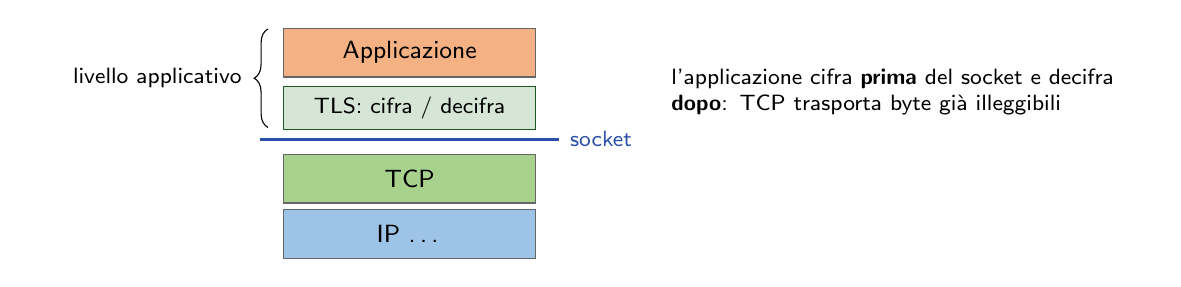
\begin{tikzpicture}[every node/.style={font=\footnotesize\sffamily}]
  \node[lay app, minimum width=3.2cm] (a) at (0,1.9) {Applicazione};
  \node[draw=netgreen!70!black, fill=netgreen!20, minimum width=3.2cm, minimum height=0.55cm] (tls) at (0,1.2) {TLS: cifra / decifra};
  \draw[very thick, netblue] (-1.9,0.8) -- (1.9,0.8) node[right, text=netblue] {socket};
  \node[lay tra, minimum width=3.2cm] (t) at (0,0.3) {TCP};
  \node[lay net, minimum width=3.2cm] at (0,-0.4) {IP \dots};
  \draw[decorate, decoration={brace, amplitude=5pt}] (-1.8,0.95) -- (-1.8,2.2) node[midway, left=6pt, lbl, text width=2.6cm, align=right] {livello applicativo};
  \node[lbl, text width=6cm, align=left, anchor=west] at (3.2,1.4) {l'applicazione cifra \textbf{prima} del socket e decifra \textbf{dopo}: TCP trasporta byte già illeggibili};
\end{tikzpicture}
\caption{TLS non è un terzo protocollo di trasporto: è un miglioramento di TCP, implementato nel livello applicativo.}
\end{figure}

% ══════════════════════════════════════════════════════════════
\section{I protocolli di livello applicativo}
% ══════════════════════════════════════════════════════════════

\dfn{Protocollo di livello applicativo}{
    Un \textbf{protocollo applicativo} definisce come i processi di un'applicazione, in esecuzione su end
    system diversi, si scambiano i messaggi. In particolare definisce:
    \begin{enumerate}
      \item i \textbf{tipi} di messaggi scambiati (per esempio richieste e risposte);
      \item la \textbf{sintassi} dei vari tipi di messaggio: quali campi ci sono e come sono delimitati;
      \item la \textbf{semantica} dei campi: il significato dell'informazione che contengono;
      \item le \textbf{regole} che stabiliscono quando e come un processo invia messaggi e risponde.
    \end{enumerate}
}

I protocolli possono essere \textbf{aperti} (le regole sono pubbliche, tipicamente in un RFC: HTTP,
SMTP, DNS) oppure \textbf{proprietari}, deliberatamente chiusi (come quello di Skype o di molte app di
messaggistica).

\subsection{Un protocollo non è l'applicazione}

Il Web è un'applicazione; HTTP ne è \textbf{un pezzo}.

\begin{figure}[H]
\centering
\begin{tikzpicture}[every node/.style={font=\footnotesize\sffamily}]
  \node[draw=primary, thick, rounded corners, minimum width=11.5cm, minimum height=2.5cm] (web) at (0,0) {};
  \node[anchor=north west, font=\small\bfseries\sffamily, text=primary] at (web.north west) {l'applicazione Web};
  \node[draw, fill=lapp!40, rounded corners, minimum width=2.2cm, minimum height=0.9cm] (b) at (-4.2,-0.2) {browser};
  \node[draw, fill=lapp!40, rounded corners, minimum width=2.2cm, minimum height=0.9cm] (s) at (4.2,-0.2) {server Web};
  \node[draw, fill=black!8, rounded corners, minimum width=2cm, minimum height=0.6cm] at (0,0.55) {formato HTML};
  \draw[{Stealth}-{Stealth}, very thick, netred] (b) -- node[below, text=netred, font=\footnotesize\bfseries\sffamily] {protocollo HTTP} (s);
  \node[lbl, text=netred] at (0,-0.95) {l'unica parte su cui i due capi devono mettersi d'accordo};
\end{tikzpicture}
\caption{Il Web ha bisogno di un formato per i documenti (HTML), di browser e di server: HTTP fissa soltanto formato e ordine dei messaggi tra browser e server.}
\end{figure}

Lo stesso vale per il video on demand: server, fatturazione, l'app sul telefono, e \textbf{DASH} per i messaggi.
Perché insistere sulla distinzione? Perché il protocollo è \textbf{l'unica parte su cui entrambi i capi devono
concordare}: tutto il resto ciascuna parte lo costruisce come vuole.

\subsection{Protocolli applicativi comuni}

Ecco alcuni protocolli applicativi di uso comune, con il trasporto che usano:

\begin{table}[H]
\centering
\begin{tabular}{lp{8.6cm}ll}
\toprule
\textbf{Protocollo} & \textbf{Descrizione} & \textbf{Porta} & \textbf{Trasporto} \\
\midrule
DHCP & \emph{Dynamic Host Configuration Protocol}: assegna gli indirizzi IP & 67, 68 & UDP \\
DNS & \emph{Domain Name System}: traduce i nomi in indirizzi IP & 53 & UDP, TCP \\
HTTP / HTTPS & \emph{HyperText Transfer Protocol (Secure)}: trasferisce pagine Web & 80 / 443 & TCP \\
SMTP / SMTPS & \emph{Simple Mail Transfer Protocol (Secure)}: invia la posta & 25 / 465 & TCP \\
SNMP & \emph{Simple Network Management Protocol}: gestisce i dispositivi di rete & 161 & UDP \\
Telnet / SSH & \emph{Teletype Network / Secure SHell}: riga di comando su host remoti & 23 / 22 & TCP \\
FTP / FTPS & \emph{File Transfer Protocol (Secure)}: trasferisce file & 21 / 990 & TCP \\
\bottomrule
\end{tabular}
\caption{Protocolli applicativi comuni e relative porte ben note.}
\end{table}

\info{Le versioni ``Secure''}{
    Molte applicazioni scambiano informazioni sensibili (credenziali, dati personali). Sulle reti pubbliche
    i messaggi vanno protetti: da qui le varianti sicure (HTTPS, SMTPS, FTPS, SSH) di quasi ogni protocollo.
    Telnet, per esempio, trasmette tutto in chiaro, password comprese; SSH offre lo stesso servizio (una
    riga di comando remota) con tutto cifrato. Su una rete pubblica, usare la variante in chiaro è un errore.
}

% ══════════════════════════════════════════════════════════════
\section{FTP e FTPS}
% ══════════════════════════════════════════════════════════════

\dfn{FTP}{
    L'\textbf{FTP} (\emph{File Transfer Protocol}) è uno dei protocolli più antichi di Internet (prima
    versione nel 1971) e serve a \textbf{trasferire file} tra host attraverso la rete, secondo il modello
    client-server.
}

\begin{itemize}
    \item Nella versione base il trasferimento avviene \textbf{in chiaro}: nome utente, password e file
          viaggiano leggibili da chiunque intercetti il traffico. Va quindi usato in reti locali o private.
    \item La versione sicura \textbf{FTPS} (\emph{FTP Secure}) protegge nome utente e password e cifra i contenuti.
    \item Sia FTP sia FTPS hanno due componenti: il \textbf{protocollo}, che specifica i comandi (elencare,
          prendere, cancellare file, \dots), e un'\textbf{applicazione} che lo implementa, con un lato client e
          un lato server.
\end{itemize}

\subsection{Due connessioni: controllo e dati}

A differenza dei protocolli visti finora, FTP \textbf{non} trasporta comandi e dati sulla stessa connessione.
\begin{itemize}
    \item La \textbf{connessione di controllo}, sulla porta \textbf{21}, si apre per prima e resta aperta per tutta
          la sessione: solo comandi e risposte.
    \item Ogni trasferimento (un \texttt{get}, un \texttt{put}, persino un \texttt{ls}) apre una \textbf{seconda
          connessione} solo per i dati, che viene chiusa alla fine del trasferimento.
    \item Tenere il controllo separato dai dati si chiama segnalazione \textbf{fuori banda} (\emph{out-of-band}).
\end{itemize}

\begin{figure}[H]
\centering
\begin{tikzpicture}[every node/.style={font=\footnotesize\sffamily}]
  \begin{scope}
    \node[font=\small\bfseries\sffamily] at (3,1.5) {Modalità attiva};
    \node (c) at (0,0) {\icon[1cm]{laptop}}; \node[below=-2pt of c] {client};
    \node (s) at (6,0) {\icon[0.75cm]{server}}; \node[below=-2pt of s] {server};
    \draw[-{Stealth}, very thick, netblue] (0.7,0.45) -- node[above] {controllo: il client apre (porta 21)} (5.6,0.45);
    \draw[-{Stealth}, very thick, netgreen!60!black] (5.6,-0.25) -- node[below] {dati: il \textbf{server} apre (dalla porta 20)} (0.7,-0.25);
    \node[draw=netred, fill=netred!8, rounded corners, text width=5.2cm, align=center] at (3,-1.75) {un client dietro NAT o firewall \textbf{non} è raggiungibile dall'esterno: la connessione dati fallisce};
  \end{scope}
  \begin{scope}[xshift=8.2cm]
    \node[font=\small\bfseries\sffamily] at (3,1.5) {Modalità passiva};
    \node (c) at (0,0) {\icon[1cm]{laptop}}; \node[below=-2pt of c] {client};
    \node (s) at (6,0) {\icon[0.75cm]{server}}; \node[below=-2pt of s] {server};
    \draw[-{Stealth}, very thick, netblue] (0.7,0.45) -- node[above] {controllo: il client apre (porta 21)} (5.6,0.45);
    \draw[-{Stealth}, very thick, netgreen!60!black] (0.7,-0.25) -- node[below] {dati: apre \textbf{ancora il client}} (5.6,-0.25);
    \node[draw=netgreen!70!black, fill=netgreen!8, rounded corners, text width=5.2cm, align=center] at (3,-1.75) {esiste proprio per questo: il client apre entrambe le connessioni};
  \end{scope}
\end{tikzpicture}
\caption{Chi apre la connessione dati? In modalità attiva il server si ricollega al client; in modalità passiva è il client ad aprire entrambe.}
\end{figure}

\subsection{Una sessione FTP}

Sul server un \textbf{demone} attende in background le connessioni; sul client si usa il programma \texttt{ftp}.

\begin{lstlisting}[language=bash]
$ sudo apt install vsftpd          # lato server, una volta sola
$ systemctl status vsftpd          # il demone e' in esecuzione?

$ ftp 143.225.161.30               # lato client
Name: student
Password:
230 Login successful.
ftp> ls                            # da qui in poi, il prompt ftp>
ftp> get report.pdf                # dal server al client
226 Transfer complete.
ftp> bye                           # bye o quit, non exit
\end{lstlisting}

I codici numerici (230, 226) sono le \textbf{risposte} del server sulla connessione di controllo: 230 conferma
l'accesso, 226 la fine del trasferimento.

\info{Il demone}{
    Il lato server è implementato come \textbf{demone} (\emph{daemon}): un programma che gira in background
    e resta in attesa che i client si connettano. Quasi ogni server che scriverete in questo corso ha questa
    forma: un demone, in attesa.
}

\begin{table}[H]
\centering
\begin{tabular}{ll}
\toprule
\textbf{Comando} & \textbf{Effetto} \\
\midrule
\texttt{help} & elenca i comandi FTP disponibili \\
\texttt{cd} / \texttt{lcd} & cambia directory sulla macchina remota / locale \\
\texttt{ls} & mostra file e directory nella directory remota corrente \\
\texttt{pwd} & stampa la directory di lavoro remota \\
\texttt{mkdir} / \texttt{rmdir} & crea / rimuove una directory remota \\
\texttt{delete} & cancella un file nella directory remota \\
\texttt{get} & copia un file dal server alla macchina locale (\emph{download}) \\
\texttt{put} & copia un file dalla macchina locale al server (\emph{upload}) \\
\bottomrule
\end{tabular}
\caption{I comandi FTP principali.}
\end{table}

Due comandi, \texttt{get} e \texttt{put}, sono la ragione per cui il protocollo esiste; il resto è navigazione.
Attenzione a \texttt{lcd}: è l'unico che agisce sulla \textbf{vostra} macchina.

% ══════════════════════════════════════════════════════════════
\section{Riepilogo}
% ══════════════════════════════════════════════════════════════

\riepilogo{
\begin{itemize}
    \item Un'applicazione di rete è fatta di programmi su \textbf{end system diversi}; il nucleo della rete
          non esegue applicazioni.
    \item Architetture: \textbf{client-server} (server sempre attivo, indirizzo noto) e \textbf{P2P} (peer
          intermittenti, scalabile); nella pratica spesso \textbf{ibride}.
    \item Comunicano \textbf{processi}, attraverso i \textbf{socket}: l'interfaccia tra applicazione e trasporto.
    \item Un processo si raggiunge con \textbf{indirizzo IP} (host, livello di rete) + \textbf{numero di porta}
          (processo, livello di trasporto).
    \item Un indirizzo IP appartiene a un'\textbf{interfaccia}; \texttt{127.0.0.1} indica l'host stesso; il DNS
          traduce i nomi (per le persone) in indirizzi (per la rete).
    \item Le applicazioni chiedono al trasporto affidabilità, throughput, tempi, sicurezza; Internet offre
          \textbf{TCP} (connessione, affidabile) e \textbf{UDP} (senza connessione, minimale), e garantisce solo
          l'affidabilità: niente throughput, tempi o sicurezza (TLS si aggiunge sopra TCP, a livello applicativo).
    \item Un protocollo applicativo definisce tipi, sintassi, semantica dei messaggi e regole di scambio, ed è
          solo \textbf{un pezzo} dell'applicazione.
    \item \textbf{FTP} usa due connessioni: controllo (porta 21, per tutta la sessione) e dati (una per
          trasferimento); modalità attiva e passiva.
\end{itemize}
}
  % Architetture e servizi
  \chapter{Il Web e il protocollo HTTP}

% ══════════════════════════════════════════════════════════════
\section{Dal Web a HTTP}
% ══════════════════════════════════════════════════════════════

Fino ai primi anni '90 Internet era usata soprattutto da ricercatori, docenti e studenti
universitari: per collegarsi a host remoti (Telnet), trasferire file (FTP), leggere e inviare
news e posta elettronica. Applicazioni utilissime, ma che lasciavano Internet sconosciuta fuori
dal mondo accademico. Nei primi anni '90 arrivò il \textbf{World Wide Web}, la prima applicazione
Internet a conquistare il grande pubblico.

\dfn{World Wide Web}{
    Il \textbf{World Wide Web} (WWW, o semplicemente Web) è una collezione di informazioni
    (documenti, immagini, video, audio, \dots) accessibili attraverso Internet secondo uno specifico
    protocollo, l'\textbf{HTTP} (\emph{HyperText Transfer Protocol}).
}

La comunicazione HTTP è tipicamente \textbf{client-server}:

\begin{itemize}
    \item un \textbf{programma client} traduce le richieste dell'utente in messaggi HTTP: è implementato
          nei \textbf{browser} (Chrome, Firefox, Edge, Safari, \dots);
    \item un \textbf{programma server} esegue la richiesta HTTP e restituisce una risposta HTTP.
\end{itemize}

\begin{figure}[H]
\centering
\begin{tikzpicture}[every node/.style={font=\footnotesize\sffamily}]
  \node (srv) at (0,0) {\icon[0.9cm]{server}};
  \node[below=-1pt of srv, align=center] {server Web\\(per esempio Apache)};
  \node (c1) at (-5,1.3) {\icon[1.1cm]{pc}}; \node[below=-2pt of c1] {PC con Firefox};
  \node (c2) at (5,1.3) {\icon[1.2cm]{laptop}}; \node[below=-2pt of c2] {laptop con Safari};
  \node (c3) at (4.2,-1.6) {\icon[0.8cm]{smartphone}}; \node[below=-2pt of c3] {smartphone con Chrome};
  \foreach \c/\sx in {c1/-0.5, c2/0.5, c3/0.4} {
    \draw[msg, netblue, shorten <=14pt, shorten >=14pt] ([yshift=4pt]\c.center) -- ([yshift=4pt, xshift=\sx cm]srv.center);
    \draw[msg, netgreen, shorten <=14pt, shorten >=14pt] ([yshift=-4pt, xshift=\sx cm]srv.center) -- ([yshift=-4pt]\c.center);
  }
  \draw[msg, netblue] (-6.2,-2.2) -- ++(0.8,0) node[right, text=netblue] {richiesta HTTP};
  \draw[msg, netgreen] (-6.2,-2.7) -- ++(0.8,0) node[right, text=netgreen] {risposta HTTP};
\end{tikzpicture}
\caption{Client diversi, con browser diversi, parlano con lo stesso server perché condividono il protocollo HTTP.}
\end{figure}

HTTP definisce principalmente due cose: la \textbf{struttura dei messaggi} e \textbf{come client e
server se li scambiano}.

\warning{Cosa HTTP non definisce}{
    HTTP non stabilisce come vadano implementati client e server, né come i contenuti vadano
    \textbf{visualizzati}. Il modo in cui una pagina appare dipende dal browser: due browser possono
    mostrare la stessa pagina in modi un po' diversi (uno aspetta che sia tutta caricata, l'altro la
    mostra pezzo per pezzo).
}

Il Web e i suoi protocolli sono la piattaforma di applicazioni come YouTube, la posta via Web
(Gmail) e gran parte delle app per dispositivi mobili, social network compresi.

\begin{figure}[H]
\centering
\begin{tikzpicture}[every node/.style={font=\footnotesize\sffamily}]
  \node (c) at (0,0) {\icon[1cm]{laptop}};
  \node[lay app, minimum width=2.4cm] (ca) at (0,-1.1) {browser};
  \node[lay tra, minimum width=2.4cm] (ct) at (0,-1.72) {};
  \node[lbl] at (0,-2.3) {[\dots] resto della pila};
  \node (s) at (7,0) {\icon[0.7cm]{server}};
  \node[lay app, minimum width=2.4cm] (sa) at (7,-1.1) {server Web};
  \node[lay tra, minimum width=2.4cm] (st) at (7,-1.72) {};
  \node[lbl] at (7,-2.3) {[\dots] resto della pila};
  \draw[{Stealth}-{Stealth}, thick, netred] (ca) -- node[above, text=netred] {HTTP} (sa);
  \draw[{Stealth}-{Stealth}, thick, netred] (ct) -- node[below, text=netred] {TCP (o UDP)} (st);
  \node[anchor=west] at (9,-1.1) {livello applicativo};
  \node[anchor=west] at (9,-1.72) {livello di trasporto};
\end{tikzpicture}
\caption{HTTP è il protocollo tra browser e server Web; sotto, il trasporto è affidato a TCP (o, con HTTP/3, a UDP).}
\end{figure}

% ══════════════════════════════════════════════════════════════
\section{Le URL}
% ══════════════════════════════════════════════════════════════

\dfn{Risorsa e URL}{
    Le informazioni sul Web si chiamano \textbf{risorse} (o \textbf{oggetti}) e sono identificate da un
    \textbf{URL} (\emph{Uniform Resource Locator}), una stringa con la forma generale:
    \begin{center}
    \texttt{[protocollo]://[userinfo@][host][:porta][/percorso][?query][\#frammento]}
    \end{center}
}

\begin{figure}[H]
\centering
\begin{tikzpicture}[every node/.style={font=\ttfamily\large, inner sep=2pt}]
  \node[fill=lapp!60] (p) at (0,0) {https};
  \node[right=0pt of p] (s1) {://};
  \node[fill=lnet!60, right=0pt of s1] (h) {en.wikipedia.org};
  \node[fill=ltra!60, right=0pt of h] (pt) {:443};
  \node[fill=llink!80, right=0pt of pt] (pa) {/w/index.php};
  \node[fill=netred!20, right=0pt of pa] (q) {?title=SSC\_Napoli};
  \node[fill=lphy, right=0pt of q] (f) {\#Storia};
  \foreach \n/\t/\d in {p/protocollo/0.5, h/{host (nome o indirizzo IP)}/0.5, pt/porta/1.2, pa/percorso/0.5, q/query/1.2, f/frammento/0.5}
     \draw[{Stealth}-, thin] (\n.south) -- ++(0,-\d) node[below, font=\small\sffamily] {\t};
\end{tikzpicture}
\caption{Anatomia di un URL.}
\end{figure}

\begin{itemize}
    \item \texttt{[protocollo]}: il protocollo con cui accedere alla risorsa (HTTP, HTTPS, FTP, \dots).
    \item \texttt{[userinfo]} (opzionale): informazioni sull'utente, come \texttt{nome:password@}. È
          \textbf{deprecato} per ovvi motivi di sicurezza.
    \item \texttt{[host]}: il nome o l'indirizzo IP del server.
    \item \texttt{[porta]} (opzionale): la porta da usare; di solito si ricava dal protocollo (80 per HTTP,
          443 per HTTPS).
    \item \texttt{[percorso]}: dove si trova la risorsa dentro il server (\texttt{/percorso/della/risorsa}).
    \item \texttt{[query]}: preceduta da \texttt{?}, specifica eventuali richieste (parametri).
    \item \texttt{[frammento]}: preceduto da \texttt{\#}, identifica un elemento dentro la risorsa (una
          sezione, un modulo).
\end{itemize}

\begin{esempio}{Due URL scomposti}
\texttt{http://www.someSchool.edu/someDepartment/picture1.gif}
\begin{itemize}
    \item protocollo: \texttt{http}; host: \texttt{www.someSchool.edu}; percorso: \texttt{/someDepartment/picture1.gif}.
\end{itemize}
\texttt{https://en.wikipedia.org/w/index.php?title=SSC\_Napoli}
\begin{itemize}
    \item protocollo: \texttt{https}; host: \texttt{en.wikipedia.org}; percorso: \texttt{/w/index.php};
          query: \texttt{?title=SSC\_Napoli}.
\end{itemize}
In questo caso la query produce la stessa pagina di \texttt{https://en.wikipedia.org/wiki/SSC\_Napoli}.
\end{esempio}

\subsection{Pagine e oggetti}

La maggior parte delle pagine Web è formata da un \textbf{file HTML di base} (\emph{HyperText Markup
Language}) e da vari \textbf{riferimenti} ad altri oggetti (immagini, video, script, fogli di stile),
ciascuno con il proprio URL.

\begin{esempio}{Quanti oggetti ha una pagina}
Una pagina con un testo HTML e cinque immagini JPEG ha \textbf{sei oggetti}: il file HTML di base più le
cinque immagini. Il browser riceve prima l'HTML, vi trova i riferimenti alle immagini e le chiede una a una.
\end{esempio}

Una pagina, quindi, non è un trasferimento ma \textbf{diversi} trasferimenti: ed è proprio il modo di
organizzarli il tema del resto del capitolo.

\subsection{Prima del primo messaggio HTTP}

Tra il momento in cui si preme Invio e quello in cui parte la prima richiesta succedono già parecchie cose:

\begin{enumerate}
    \item il browser \textbf{scompone l'URL}: protocollo, host, porta, percorso;
    \item l'host è un \textbf{nome}, e verso un nome non si può aprire nessuna connessione: il \textbf{DNS}
          fornisce l'indirizzo IP corrispondente (lo vedremo nel capitolo dedicato);
    \item solo a questo punto si apre una \textbf{connessione TCP} verso quell'indirizzo, sulla porta 80 o 443;
    \item su quella connessione viaggia la prima \textbf{richiesta HTTP}, con il percorso;
    \item il browser legge l'HTML, trova gli oggetti a cui rimanda e ricomincia.
\end{enumerate}

\info{Il tempo che non contiamo}{
    Anche la risoluzione del nome costa tempo, ma nei conti in RTT che seguono non viene mai inclusa:
    si parte sempre da quando l'indirizzo del server è già noto.
}

% ══════════════════════════════════════════════════════════════
\section{Come funziona HTTP}
% ══════════════════════════════════════════════════════════════

HTTP definisce come i client Web chiedono oggetti ai server Web e come i server li trasferiscono.
Quando l'utente chiede un oggetto (per esempio cliccando un link), il browser invia messaggi di
\textbf{richiesta HTTP} per gli oggetti della pagina; il server risponde con messaggi di
\textbf{risposta HTTP} che contengono gli oggetti.

HTTP evolve continuamente per bilanciare affidabilità e prestazioni:

\begin{figure}[H]
\centering
\begin{tikzpicture}[every node/.style={font=\footnotesize\sffamily}]
  \foreach \x/\v/\y/\c in {0/{HTTP/1.0}/1996/lnet, 3.3/{HTTP/1.1}/1997/lnet, 6.6/{HTTP/2}/2015/ltra, 9.9/{HTTP/3}/2022/lapp} {
    \node[signal, signal to=east, fill=\c, draw=black!50, minimum width=3.1cm, minimum height=0.9cm, align=center] at (\x,0) {\bfseries \v\\\y};
  }
  \node[lbl, text width=3cm] at (0,-0.9) {connessioni non persistenti};
  \node[lbl, text width=3cm] at (3.3,-0.9) {connessioni persistenti};
  \node[lbl, text width=3cm] at (6.6,-0.9) {richieste intercalate e priorità};
  \node[lbl, text width=3cm] at (9.9,-0.9) {su UDP con QUIC};
\end{tikzpicture}
\caption{Le versioni di HTTP.}
\end{figure}

\subsection{Il protocollo di trasporto sottostante}

HTTP usa principalmente \textbf{TCP} come protocollo di trasporto; dal 2022, con \textbf{HTTP/3}, può
usare anche \textbf{UDP} (circa il 30\% del traffico HTTP viaggia oggi su UDP).

\begin{enumerate}
    \item Il client HTTP \textbf{apre una connessione} TCP con il server.
    \item Stabilita la connessione, browser e server comunicano attraverso i loro \textbf{socket}: il client
          scrive richieste nel proprio socket e legge risposte dal proprio socket; il server fa il contrario.
\end{enumerate}

Perché storicamente TCP? Perché offre servizi utilissimi, soprattutto il \textbf{trasferimento
affidabile}: garantisce che richieste e risposte arrivino integre a destinazione (se possibile). Ma i
servizi di TCP rallentano la comunicazione: per questo HTTP/3 usa UDP con sopra il protocollo
\textbf{QUIC} (\emph{Quick UDP Internet Connections}), che reimplementa l'affidabilità sopra UDP ed è
stimato essere circa il 30\% più veloce.

\info{Il vantaggio della stratificazione, visto da HTTP}{
    Qui si vede uno dei grandi vantaggi dell'architettura a strati: le applicazioni HTTP non devono
    preoccuparsi di raggiungibilità, perdite di dati, ritrasmissioni. Possono essere più semplici, sia
    logicamente sia computazionalmente, delegando gran parte del lavoro agli strati sottostanti.
}

% ══════════════════════════════════════════════════════════════
\section{HTTP è stateless}
% ══════════════════════════════════════════════════════════════

La semplicità è fondamentale per un server che riceve moltissime richieste al secondo (in media
un server gestisce circa 1000 richieste HTTP al secondo, e l'infrastruttura di un grande motore di
ricerca centinaia di migliaia di interrogazioni al secondo).

\dfn{Protocollo stateless}{
    HTTP è \textbf{senza stato} (\emph{stateless}): il server \textbf{non conserva alcuna informazione}
    sulle interazioni passate con un certo client.
}

\begin{esempio}{La stessa richiesta due volte}
Se un client chiede lo stesso oggetto due volte di seguito, il server non considera la seconda
richiesta ridondante: rimanda semplicemente l'oggetto, perché ha completamente dimenticato la prima.
\end{esempio}

Non tutte le applicazioni sono stateless: molte sono \textbf{stateful} (con stato). Vedremo come HTTP
riesca comunque a ``ricordarsi'' degli utenti usando i \textbf{cookie}.

% ══════════════════════════════════════════════════════════════
\section{Connessioni persistenti e non persistenti}
% ══════════════════════════════════════════════════════════════

Client e server possono comunicare a lungo, scambiandosi molte coppie richiesta--risposta (una di
seguito all'altra, a intervalli regolari o in modo intermittente). Con un trasporto orientato alla
connessione (TCP o QUIC) ci sono due possibilità.

\dfn{Connessioni persistenti e non persistenti}{
    \begin{itemize}
      \item \textbf{Connessione non persistente}: per \textbf{ogni} coppia richiesta--risposta si apre una
            \textbf{nuova} connessione, che viene chiusa subito dopo.
      \item \textbf{Connessione persistente}: tutte le richieste e le risposte viaggiano sulla
            \textbf{stessa} connessione.
    \end{itemize}
}

Le prime versioni di HTTP (HTTP/1.0) usavano per default connessioni non persistenti; oggi il default
sono le connessioni persistenti, ma client e server possono essere configurati per usare quelle non
persistenti.

\subsection{Esempio di connessione non persistente}

Chiediamo una pagina fatta di un file HTML di base e \textbf{10 immagini JPEG}, tutte sullo stesso
server, all'URL \url{http://www.someschool.edu/someDepartment/home.index}.

\begin{enumerate}
    \item Il client HTTP \textbf{apre una connessione TCP} verso \texttt{www.someschool.edu} sulla porta
          \textbf{80}: ci sono ora due socket, uno sul client e uno sul server.
    \item Il client invia nel proprio socket una \textbf{richiesta HTTP} che contiene il percorso
          \texttt{/someDepartment/home.index}.
    \item Il server riceve la richiesta, recupera l'oggetto (da RAM o disco), lo incapsula in una
          \textbf{risposta HTTP} e la invia nel proprio socket.
    \item Il server dice a TCP di \textbf{chiudere} la connessione; TCP la chiuderà davvero quando sarà
          sicuro che il client ha ricevuto la risposta integra.
    \item Il client riceve la risposta e la connessione termina. Il messaggio dice che l'oggetto è un file
          HTML: il client lo estrae, lo esamina e trova i riferimenti ai 10 JPEG.
    \item I passi 1--4 vengono ripetuti \textbf{per ciascuna delle 10 immagini}.
\end{enumerate}

\begin{figure}[H]
\centering
\begin{tikzpicture}[every node/.style={font=\footnotesize\sffamily}]
  \node (c) at (0,0) {\icon[1.1cm]{pc}}; \node[below=-2pt of c] {client};
  \node (s) at (8,0) {\icon[0.8cm]{server}}; \node[below=-2pt of s] {server};
  \foreach \i/\y/\t in {1/1.5/HTML, 2/0.9/JPEG 1, 3/0.3/JPEG 2, 11/-1.2/JPEG 10} {
    \draw[{Stealth}-{Stealth}, thick, netblue] (1,\y) -- node[above=-1pt, fill=white, inner sep=1pt] {connessione TCP n.~\i: \t} (7,\y);
  }
  \node at (4,-0.45) {$\vdots$};
\end{tikzpicture}
\caption{Con connessioni non persistenti servono 11 connessioni TCP (e 11 coppie di socket) per una pagina di 11 oggetti.}
\end{figure}

Poiché la connessione non sopravvive tra un oggetto e l'altro, servono \textbf{11 connessioni TCP} per
trasferire la pagina, e gli elementi possono arrivare in momenti diversi.

\subsection{Connessioni in sequenza e in parallelo}

Le connessioni possono essere aperte \textbf{in sequenza} o \textbf{in parallelo}. Nell'esempio, una volta
ricevuto l'HTML e scoperto che servono 10 immagini, il browser può scaricarle tutte
contemporaneamente.

\begin{itemize}
    \item I browser moderni permettono di configurare il grado di parallelismo: di solito aprono \textbf{da 5
          a 10 connessioni TCP parallele}, ciascuna con una sola transazione richiesta--risposta.
    \item Le connessioni parallele \textbf{accorciano il tempo di risposta} ma \textbf{aumentano il costo
          computazionale}.
    \item Anche con il parallelismo, aprire tante connessioni TCP ha un costo in tempo non trascurabile.
\end{itemize}

% ══════════════════════════════════════════════════════════════
\section{Il costo in RTT}
% ══════════════════════════════════════════════════════════════

È difficile stimare con precisione i tempi su Internet. Si può però misurare il costo di una richiesta
in \textbf{RTT}.

\dfn{Round-Trip Time (RTT)}{
    L'\textbf{RTT} è il tempo impiegato da un \textbf{piccolo pacchetto} per andare dal client al server e
    \textbf{tornare} al client.
}

\subsection{Il three-way handshake}

Con un trasporto orientato alla connessione come TCP, prima di scambiare dati si esegue il
\textbf{three-way handshake} (stretta di mano a tre vie):

\begin{figure}[H]
\centering
\begin{tikzpicture}[yscale=0.85, every node/.style={font=\footnotesize\sffamily}]
  \timeline{c}{0}{Client}{5.2}
  \timeline{s}{6}{Server}{5.2}
  \draw[msg, netblue] (0,-0.4) -- node[above, sloped] {1. ``vorrei aprire una connessione'' (SYN)} (6,-1.4);
  \draw[msg, netblue] (6,-1.6) -- node[above, sloped] {2. ``ricevuto, sono pronto'' (SYN-ACK)} (0,-2.6);
  \draw[msg, netgreen] (0,-2.8) -- node[above, sloped] {3. ``ricevuto'' + richiesta HTTP (ACK)} (6,-3.8);
  \draw[msg, netgreen, very thick] (6,-4.0) -- node[above, sloped] {risposta: il file HTML} (0,-5.0);
  \draw[decorate, decoration={brace, amplitude=5pt, mirror}] (-0.2,-0.4) -- (-0.2,-2.6) node[midway, left=6pt] {1 RTT};
  \draw[decorate, decoration={brace, amplitude=5pt, mirror}] (-0.2,-2.8) -- (-0.2,-5.0) node[midway, left=6pt] {1 RTT};
  \draw[decorate, decoration={brace, amplitude=5pt}] (6.2,-4.0) -- (6.2,-4.4) node[midway, right=6pt, text width=2.6cm, align=left] {tempo di trasmissione del file};
  \node[right, text=netgreen!60!black] at (6.3,-3.1) {connessione stabilita};
\end{tikzpicture}
\caption{Richiesta di un file HTML con connessione non persistente: circa 2 RTT più il tempo di trasmissione del file.}
\end{figure}

\begin{enumerate}
    \item Il client invia un piccolo segmento TCP per segnalare che vuole aprire una connessione.
    \item Il server conferma e risponde con un piccolo segmento TCP.
    \item Il client conferma a sua volta.
\end{enumerate}

Dal punto di vista degli RTT, i primi due passi dell'handshake richiedono \textbf{1 RTT}. Un
handshake analogo avviene anche quando la connessione viene chiusa.

\subsection{Il conto totale}

\begin{itemize}
    \item In HTTP il client invia la \textbf{richiesta} insieme al terzo passo dell'handshake (la conferma).
    \item Quando la richiesta arriva, il server invia il file HTML: la coppia richiesta--risposta costa
          \textbf{un altro RTT}.
\end{itemize}

\dfn{Tempo di risposta con connessione non persistente}{
    $$T_{\text{risposta}} \approx \underbrace{1\ \text{RTT}}_{\text{apertura TCP}} + \underbrace{1\ \text{RTT}}_{\text{richiesta e risposta}} + t_{\text{trasmissione del file}} = 2\ \text{RTT} + t_{\text{trasmissione}}$$
}

\begin{esempio}{La stessa pagina, contata in quattro modi}
La pagina con l'HTML e 10 immagini JPEG (11 oggetti), senza perdite e con tempi di trasmissione
trascurabili, come nelle slide:

\begin{center}
\renewcommand{\arraystretch}{1.3}
\begin{tabular}{p{6.2cm}p{4.6cm}r}
\toprule
\textbf{Modalità} & \textbf{Conto} & \textbf{RTT} \\
\midrule
Non persistente, un oggetto alla volta & $2 \times 11$ & \textbf{22} \\
Non persistente, 5 connessioni in parallelo & 2 per l'HTML, poi due turni da 2 per le 10 immagini & \textbf{6} \\
Persistente, senza pipelining & 1 per aprire, poi 1 per ogni oggetto & \textbf{12} \\
Persistente con pipelining & 1 per aprire, 1 per l'HTML, 1 per le 10 immagini insieme & \textbf{3} \\
\bottomrule
\end{tabular}
\end{center}

Con RTT $= 50$ ms si va da $22 \times 50 = 1{,}1$ s a $3 \times 50 = 0{,}15$ s. Stessa pagina, stesso server,
stessa distanza: tutto ciò che sta fra 22 e 3 dipende solo da \textbf{come vengono gestite le connessioni}.
\end{esempio}

% ══════════════════════════════════════════════════════════════
\section{Connessioni persistenti e pipelining}
% ══════════════════════════════════════════════════════════════

Nelle connessioni \textbf{persistenti} il server \textbf{lascia aperta} la connessione TCP dopo aver
inviato una risposta.

\begin{itemize}
    \item Richieste e risposte successive tra lo stesso client e lo stesso server viaggiano sulla stessa
          connessione: l'intera pagina dell'esempio (HTML + 10 immagini) passa su \textbf{una sola}
          connessione TCP.
    \item Anche più pagine dello stesso server possono essere inviate sulla stessa connessione.
    \item L'handshake si paga \textbf{una volta sola}: ogni oggetto dopo il primo costa \textbf{1 RTT} invece di 2.
    \item Il server chiude la connessione quando resta inutilizzata per un tempo configurabile (\emph{timeout}).
\end{itemize}

\dfn{Pipelining}{
    Con il \textbf{pipelining} le richieste di più oggetti vengono inviate \textbf{una dietro l'altra},
    senza aspettare le risposte alle richieste precedenti. Da HTTP/2 richieste e risposte possono anche
    essere \textbf{intercalate} sulla stessa connessione, con un meccanismo di \textbf{priorità}. Le
    connessioni persistenti con pipelining sono oggi la modalità di default.
}

\begin{figure}[H]
\centering
\begin{tikzpicture}[yscale=0.52, every node/.style={font=\scriptsize\sffamily}]
  % non persistente
  \begin{scope}
    \node[font=\footnotesize\bfseries\sffamily] at (1.5,1) {Non persistente};
    \draw[thick] (0,0) -- (0,-15); \draw[thick] (3,0) -- (3,-15);
    \foreach \k/\t in {0/file 1, 5/file 2, 10/file 3} {
      \draw[msg, netblue] (0,-\k-0.2) -- (3,-\k-0.9); \draw[msg, netblue] (3,-\k-1.0) -- (0,-\k-1.7); \draw[msg, netblue] (0,-\k-1.8) -- (3,-\k-2.5);
      \draw[msg, netgreen, very thick] (3,-\k-2.6) -- node[above, sloped] {\t} (0,-\k-3.8);
      \node[text=netred] at (1.5,-\k-4.4) {chiusura};
    }
  \end{scope}
  % persistente
  \begin{scope}[xshift=5cm]
    \node[font=\footnotesize\bfseries\sffamily] at (1.5,1) {Persistente};
    \draw[thick] (0,0) -- (0,-15); \draw[thick] (3,0) -- (3,-15);
    \draw[msg, netblue] (0,-0.2) -- (3,-0.9); \draw[msg, netblue] (3,-1.0) -- (0,-1.7); \draw[msg, netblue] (0,-1.8) -- (3,-2.5);
    \draw[msg, netgreen, very thick] (3,-2.6) -- node[above, sloped] {file 1} (0,-3.8);
    \draw[msg, netblue] (0,-4.0) -- node[above, sloped] {richiesta 2} (3,-4.8);
    \draw[msg, netgreen, very thick] (3,-4.9) -- node[above, sloped] {file 2} (0,-6.1);
    \draw[msg, netblue] (0,-6.3) -- node[above, sloped] {richiesta 3} (3,-7.1);
    \draw[msg, netgreen, very thick] (3,-7.2) -- node[above, sloped] {file 3} (0,-8.4);
  \end{scope}
  % pipelining
  \begin{scope}[xshift=10cm]
    \node[font=\footnotesize\bfseries\sffamily] at (1.5,1) {Pipelining};
    \draw[thick] (0,0) -- (0,-15); \draw[thick] (3,0) -- (3,-15);
    \draw[msg, netblue] (0,-0.2) -- (3,-0.9); \draw[msg, netblue] (3,-1.0) -- (0,-1.7); \draw[msg, netblue] (0,-1.8) -- (3,-2.5);
    \draw[msg, netgreen, very thick] (3,-2.6) -- node[above, sloped] {file 1} (0,-3.8);
    \draw[msg, netred] (0,-4.0) -- (3,-4.8); \draw[msg, netred] (0,-4.3) -- (3,-5.1);
    \node[text=netred, rotate=-15] at (1.4,-3.7) {richieste 2 e 3};
    \draw[msg, netgreen, very thick] (3,-5.2) -- (0,-6.4); \draw[msg, netgreen, very thick] (3,-5.5) -- (0,-6.7);
    \node[text=netgreen!60!black] at (1.5,-7.3) {file 2 e 3};
  \end{scope}
  \draw[-{Stealth}, thick, black!50] (-0.7,0) -- node[left, rotate=90, anchor=south] {tempo} (-0.7,-15);
\end{tikzpicture}
\caption{Confronto indicativo degli RTT necessari per richiedere 3 file nelle tre modalità.}
\end{figure}

\subsection{Confronto}

\begin{table}[H]
\centering
\begin{tabular}{p{7cm}p{7cm}}
\toprule
\textbf{Persistente} & \textbf{Non persistente} \\
\midrule
\itick\ più veloce, soprattutto con il pipelining & \itick\ semplice da implementare, in perfetta sintonia con la natura stateless di HTTP \\
\itick\ richiede meno risorse (soprattutto memoria) & \icross\ richiede più risorse: per ogni connessione vanno allocati buffer e variabili TCP su client e server \\
\icross\ più complessa da implementare, specie con il pipelining & \icross\ più lenta: 1--2 RTT in più per ogni richiesta \\
\icross\ la connessione può restare aperta anche se inutilizzata: il server la chiude dopo un \emph{timeout} & \itick\ le connessioni non restano mai aperte inutilmente \\
\bottomrule
\end{tabular}
\caption{Connessioni persistenti e non persistenti a confronto.}
\end{table}

Lo scambio è quello di sempre: la connessione già aperta è veloce, ma è una risorsa tenuta occupata per
qualcuno che potrebbe non tornare più.

\subsection{La connessione che si chiude mentre la usi}

Che cosa succede se il server chiude per timeout una connessione persistente \textbf{proprio mentre} il
client la sta riusando?

\begin{itemize}
    \item Il server chiude da solo una connessione inattiva, senza chiedere nulla al client.
    \item Una richiesta scritta in quello stesso istante si perde con la connessione: nessuna risposta, e
          nessun errore da parte del protocollo.
    \item Un client che riusa una connessione inattiva deve quindi essere pronto ad \textbf{aprirne una nuova}
          e a \textbf{reinviare} la richiesta.
\end{itemize}

\warning{Ripetere deve essere innocuo}{
    Reinviare una richiesta è sicuro solo se ripeterla non fa danni. È uno dei motivi per cui ci si aspetta
    che una \texttt{GET} \textbf{non modifichi} nulla sul server: chiedere due volte la stessa pagina va bene,
    pagare due volte lo stesso ordine no.
}

% ══════════════════════════════════════════════════════════════
\section{HTTP/2 e HTTP/3}
% ══════════════════════════════════════════════════════════════

\subsection{Il blocco in testa alla fila}

Perché un oggetto grande può rallentare dieci oggetti piccoli? Prendiamo una pagina con un video pesante
in alto e molti piccoli oggetti sotto, una sola connessione persistente e un collegamento lento lungo il
percorso.

\dfn{Head-of-line blocking}{
    Il video occupa la connessione, e i piccoli oggetti, già pronti, aspettano dietro di lui: è il
    \textbf{blocco in testa alla fila} (\emph{head-of-line blocking}, HOL).
}

I browser aggirano il problema aprendo \textbf{fino a sei connessioni parallele}. Così, però, si prendono
anche una fetta più grande del collegamento più lento, perché TCP divide la banda in parti uguali fra le
\textbf{connessioni}, non fra le pagine. Eliminare quelle connessioni parallele senza pagare il blocco è lo
scopo di HTTP/2.

\subsection{HTTP/2: frame intercalati su una sola connessione}

\begin{itemize}
    \item Un sotto-livello di \textbf{framing} spezza ogni messaggio in piccoli \textbf{frame}: l'intestazione
          in uno, il corpo in altri, tutti in codifica \textbf{binaria}.
    \item I frame di risposte diverse vengono \textbf{intercalati} sulla stessa connessione e riassemblati
          dall'altra parte.
    \item Metodi, codici di stato, URL e campi di intestazione \textbf{non cambiano}: cambia solo il modo in
          cui i dati sono formattati e trasportati.
\end{itemize}

\begin{figure}[H]
\centering
\begin{tikzpicture}[every node/.style={font=\scriptsize\sffamily}, fr/.style={draw=black!50, minimum width=0.42cm, minimum height=0.42cm, inner sep=0pt}]
  \node[anchor=east, font=\footnotesize\bfseries\sffamily] at (-0.3,0.9) {HTTP/1.1};
  \foreach \i in {0,...,13} { \node[fr, fill=netred!35] at (\i*0.45,0.9) {}; }
  \node at (6.6,0.9) {\dots\ 1000 frame del video};
  \foreach \i in {0,...,3} { \node[fr, fill=lnet] at (8.0+\i*0.45,0.9) {}; }
  \node at (10.2,0.9) {\dots};
  \node[anchor=east, font=\footnotesize\bfseries\sffamily] at (-0.3,0) {HTTP/2};
  \foreach \i/\c in {0/netred!35,1/lnet,2/lnet,3/netred!35,4/lnet,5/lnet,6/netred!35,7/lnet,8/lnet,9/netred!35,10/lnet,11/lnet,12/netred!35,13/lnet} {
     \node[fr, fill=\c] at (\i*0.45,0) {}; }
  \node at (7.2,0) {\dots\ gli oggetti piccoli finiscono presto};
  \node[fr, fill=netred!35, label=right:{frame del video}] at (0.2,-0.8) {};
  \node[fr, fill=lnet, label=right:{frame degli oggetti piccoli}] at (3.6,-0.8) {};
\end{tikzpicture}
\caption{Con HTTP/1.1 gli oggetti piccoli aspettano la fine del video; con HTTP/2 i frame si alternano.}
\end{figure}

\begin{esempio}{18 frame invece di 1016}
Un video di 1000 frame e otto oggetti piccoli di 2 frame ciascuno. Con HTTP/1.1 gli oggetti piccoli arrivano
dopo il video: l'ultimo è completo dopo $1000 + 16 = 1016$ frame. Con HTTP/2, alternando un frame del video e
quelli degli oggetti piccoli, tutti gli otto oggetti sono consegnati dopo appena \textbf{18} frame
(i loro 16, più i 2 del video intercalati).
\end{esempio}

\subsection{Priorità e server push}

\begin{itemize}
    \item Il client può dare a ogni richiesta un \textbf{peso} fra 1 e 256 e dichiarare da quale altro
          messaggio dipende.
    \item Il server invia per primi i frame delle risposte a priorità più alta: il foglio di stile prima
          dell'immagine in fondo alla pagina.
    \item Con il \textbf{server push} il server legge l'HTML di base, capisce quali oggetti serviranno e li
          invia \textbf{prima che vengano richiesti}: si risparmia un RTT per ogni oggetto ``spinto'', cioè la
          richiesta che il client avrebbe comunque mandato.
\end{itemize}

\subsection{HTTP/3 e QUIC}

\dfn{QUIC}{
    \textbf{QUIC} è un protocollo di trasporto realizzato \textbf{nel livello applicativo}, sopra il
    semplicissimo UDP. Fornisce ciò che serve a HTTP e che UDP non dà: affidabilità, multiplazione di più
    flussi, controllo di flusso per ciascun flusso. \textbf{HTTP/3} è HTTP sopra QUIC.
}

\begin{itemize}
    \item Aprire una connessione richiede \textbf{meno RTT}, perché connessione e cifratura vengono negoziate
          \textbf{insieme} invece che una dopo l'altra.
    \item Un pacchetto perso blocca solo il \textbf{proprio} flusso: sparisce il blocco in testa alla fila
          che sopravviveva dentro TCP (in HTTP/2, una perdita ferma tutti i frame dietro di sé).
    \item Diversi meccanismi di HTTP/2 sono già dentro QUIC, quindi il protocollo sopra diventa più semplice.
\end{itemize}

\begin{table}[H]
\centering
\renewcommand{\arraystretch}{1.3}
\begin{tabular}{lll}
\toprule
\textbf{Versione} & \textbf{Connessioni per pagina} & \textbf{Che cosa ha introdotto} \\
\midrule
HTTP/1.0 (1996) & una per oggetto & connessioni non persistenti \\
HTTP/1.1 (1997) & una, riusata & connessioni persistenti, pipelining \\
HTTP/2 (2015) & una, con frame intercalati & framing binario, priorità, server push \\
HTTP/3 (2022) & una, su QUIC sopra UDP & apertura in meno RTT, niente HOL fra flussi \\
\bottomrule
\end{tabular}
\caption{Trent'anni di lavoro su un'unica domanda: quante connessioni, e per quanto tempo.}
\end{table}

% ══════════════════════════════════════════════════════════════
\section{Laboratorio: il primo GET con Wireshark}
% ══════════════════════════════════════════════════════════════

\subsection{Installare Wireshark}

Su Debian, Ubuntu e derivate (rispondere \emph{sì} quando si chiede se gli utenti non root possono catturare
pacchetti):

\begin{lstlisting}[language=bash]
$ sudo apt update && sudo apt install wireshark
$ sudo dpkg-reconfigure wireshark-common   # se si e' risposto no
$ sudo usermod -aG wireshark $USER         # poi uscire e rientrare
$ groups                                   # deve comparire wireshark
$ getcap /usr/bin/dumpcap
cap_net_raw,cap_net_admin=eip              # cio' che deve stampare
\end{lstlisting}

Se \texttt{getcap} non stampa nulla, bisogna assegnare a mano quelle due \emph{capability} al programma, con
\texttt{setcap}.

\subsection{Catturare un GET}

\begin{enumerate}
    \item Avviare Wireshark, senza far partire la cattura.
    \item Scrivere \texttt{http} nel filtro di visualizzazione, così da vedere solo i pacchetti HTTP.
    \item Aspettare poco più di un minuto (vedremo perché), poi avviare la cattura.
    \item Scaricare una pagina molto semplice: \texttt{\$ lynx http://www.columbia.edu/\textasciitilde fdc/sample.html}
    \item Fermare la cattura. Chiudere i dettagli Frame, Ethernet, IP e TCP, e aprire quello HTTP.
\end{enumerate}

Si vedono \textbf{due} pacchetti HTTP: la \texttt{GET} inviata dal client e il \texttt{200 OK} di risposta,
ciascuno dentro un segmento TCP, dentro un datagramma IP, dentro un frame Ethernet.

\begin{esercizio}{Domande sulla cattura}
Sulla \textbf{richiesta}: (a) quale versione di HTTP annuncia il client, e con quale risponde il server?
(b) Quali lingue il client dichiara di accettare? (c) Qual è l'indirizzo IP della propria macchina, e quello del
server?

Sulla \textbf{risposta}: (d) quale codice di stato ha restituito il server? (e) Quando è stata modificata
l'ultima volta la pagina? (f) Quanti byte di contenuto sono stati inviati? (g) Nei byte grezzi del pacchetto
ci sono righe di intestazione che l'elenco dei pacchetti non mostra?

\svolgimento
Le risposte vanno lette dalla \textbf{propria} cattura, non da qui. Dove guardare: la versione è nella prima
riga di ciascun messaggio (riga di richiesta e riga di stato); le lingue nella riga \texttt{Accept-Language};
gli indirizzi nel dettaglio IP (\emph{Source} e \emph{Destination}); il codice nella riga di stato; la data di
modifica in \texttt{Last-Modified}; i byte in \texttt{Content-Length}.

Per (e): la pagina può sembrare modificata meno di un minuto prima. Quel server aggiorna la data ogni minuto,
così che tutti scarichino una copia nuova: è il motivo dell'attesa al passo 3. Si ripeta poi con
\texttt{http://scottaaronson.com} e con un browser moderno al posto di \texttt{lynx}: che cosa cambia, e perché?
(Un browser moderno usa quasi sempre HTTPS: si veda il laboratorio del capitolo successivo.)
\end{esercizio}

% ══════════════════════════════════════════════════════════════
\section{Riepilogo}
% ══════════════════════════════════════════════════════════════

\riepilogo{
\begin{itemize}
    \item Il Web è una collezione di risorse identificate da \textbf{URL} e accessibili con \textbf{HTTP}, un
          protocollo client-server.
    \item HTTP usa \textbf{TCP} (porta 80) e, con HTTP/3, anche \textbf{UDP} con QUIC.
    \item HTTP è \textbf{stateless}: il server non ricorda le richieste precedenti.
    \item Connessioni \textbf{non persistenti}: una connessione per oggetto, circa 2 RTT + trasmissione per
          ciascuno. Connessioni \textbf{persistenti}: l'handshake si paga una volta, poi 1 RTT per oggetto; con il
          \textbf{pipelining} le richieste partono senza aspettare le risposte.
    \item \textbf{HTTP/2} intercala i frame di più risposte su una connessione (niente blocco in testa alla
          fila fra oggetti), con priorità e server push; \textbf{HTTP/3} porta tutto su \textbf{QUIC}, sopra UDP.
\end{itemize}
}
  % Web e HTTP: connessioni
  \chapter{HTTP: messaggi, cookie e caching}

Nel capitolo precedente abbiamo visto \emph{come} HTTP usa le connessioni. Ricapitoliamo e passiamo
a \emph{che cosa} si scambiano client e server.

\gbox{Ripasso: HTTP in cinque punti}{primary!70!black}{
\begin{itemize}
    \item È uno dei protocolli più usati di Internet (applicazioni Web).
    \item È \textbf{client-server} e definisce \textbf{il formato dei messaggi} e \textbf{come vengono
          scambiati} (non come si implementano client e server).
    \item Usa messaggi di \textbf{richiesta} e di \textbf{risposta}.
    \item È \textbf{stateless}: client e server non ricordano le interazioni passate.
    \item Si appoggia a un trasporto affidabile e orientato alla connessione (soprattutto TCP, di recente
          anche UDP con QUIC), con connessioni persistenti o non persistenti.
\end{itemize}
}

% ══════════════════════════════════════════════════════════════
\section{Il formato dei messaggi HTTP}
% ══════════════════════════════════════════════════════════════

HTTP ha due formati diversi per i due tipi di messaggio:

\begin{itemize}
    \item la \textbf{richiesta} specifica il \textbf{comando} (metodo) che il server deve eseguire: dammi
          una pagina, compila questo modulo, \dots;
    \item la \textbf{risposta} riporta l'\textbf{esito} del comando (successo, errore, \dots) ed eventuali
          \textbf{dati} (per esempio il file richiesto).
\end{itemize}

Entrambi sono scritti in \textbf{testo ASCII} ordinario: si leggono facilmente anche a occhio.

\subsection{Il formato della richiesta}

\begin{figure}[H]
\centering
\begin{tikzpicture}[every node/.style={font=\scriptsize\sffamily}, f/.style={field, minimum height=0.6cm}]
  % request line
  \node[f, fill=lapp, minimum width=1.6cm] (m) at (0,0) {metodo};
  \node[f, fill=white, minimum width=0.5cm, right=0pt of m] (s1) {sp};
  \node[f, fill=lnet, minimum width=3cm, right=0pt of s1] (u) {URL};
  \node[f, fill=white, minimum width=0.5cm, right=0pt of u] (s2) {sp};
  \node[f, fill=ltra, minimum width=1.6cm, right=0pt of s2] (v) {versione};
  \node[f, fill=white, minimum width=0.5cm, right=0pt of v] {cr}; \node[f, fill=white, minimum width=0.5cm] at ([xshift=0.75cm]v.east) {lf};
  % header lines
  \foreach \y in {-0.8,-1.9} {
    \node[f, fill=llink, minimum width=3.1cm, anchor=west] (h) at (-0.8,\y) {nome campo header:};
    \node[f, fill=white, minimum width=0.5cm, right=0pt of h] (sp) {sp};
    \node[f, fill=llink!50, minimum width=2.2cm, right=0pt of sp] (val) {valore};
    \node[f, fill=white, minimum width=0.5cm, right=0pt of val] (cr) {cr};
    \node[f, fill=white, minimum width=0.5cm, right=0pt of cr] {lf};
  }
  \node at (1.5,-1.35) {$\vdots$};
  \node[f, fill=white, minimum width=0.5cm, anchor=west] (bcr) at (-0.8,-2.7) {cr};
  \node[f, fill=white, minimum width=0.5cm, right=0pt of bcr] {lf};
  \node[f, fill=lphy!60, minimum width=8.8cm, minimum height=1cm, anchor=north west] at (-0.8,-3.1) {corpo (\emph{entity body}): dati, se il metodo li prevede};
  % labels
  \draw[decorate, decoration={brace, amplitude=5pt}] (-1.1,-0.3) -- (-1.1,0.3) node[midway, left=6pt] {riga di richiesta};
  \draw[decorate, decoration={brace, amplitude=5pt}] (-1.1,-2.2) -- (-1.1,-0.5) node[midway, left=6pt] {righe di header};
  \node[left] at (-1.3,-2.7) {riga vuota};
  \node[left] at (-1.3,-3.6) {corpo};
\end{tikzpicture}
\caption{Formato generale di un messaggio di richiesta HTTP.}
\end{figure}

Il messaggio di richiesta contiene:

\begin{itemize}
    \item il \textbf{metodo}: il comando da far eseguire al server;
    \item l'\textbf{URL}: l'oggetto su cui si vuole operare;
    \item la \textbf{versione} di HTTP (per esempio \texttt{HTTP/1.1});
    \item le \textbf{righe di header}: i parametri della richiesta, in numero e tipo non fissati; ogni riga ha
          il nome e il valore del parametro. Qui si può per esempio chiedere una connessione persistente o
          no; si possono usare anche header personalizzati;
    \item il \textbf{corpo} (\emph{body}): dipende dal metodo e contiene gli eventuali dati associati al
          comando (per esempio il testo con cui compilare un modulo).
\end{itemize}

\warning{I separatori}{
    I campi sono separati da caratteri speciali: \texttt{sp} è lo \textbf{spazio}; \texttt{cr} è il
    \emph{carriage return} (\texttt{\textbackslash r}); \texttt{lf} è il \emph{line feed}
    (\texttt{\textbackslash n}). Ogni riga termina con \texttt{\textbackslash r\textbackslash n}, e una
    \textbf{riga vuota} (\texttt{\textbackslash r\textbackslash n} da solo) separa gli header dal corpo.
    Dimenticarla, quando si scrive una richiesta a mano, è l'errore più comune.
}

\subsection{I metodi HTTP}

\begin{table}[H]
\centering
\begin{tabular}{lp{12cm}}
\toprule
\textbf{Metodo} & \textbf{Uso} \\
\midrule
\texttt{GET} & \textbf{recupera} un oggetto dal server. È il metodo più usato: ogni volta che si apre una pagina si
fa una GET. Il corpo è \textbf{vuoto}. \\
\texttt{POST} & \textbf{invia informazioni} al server, per esempio il contenuto di un modulo. Il corpo contiene
i dati. \\
\texttt{HEAD} & come GET, ma il server risponde \textbf{senza l'oggetto}, con i soli header. Utile per il
debugging e per controllare se un oggetto esiste o è cambiato. \\
\texttt{PUT} & \textbf{carica} un oggetto in un certo percorso del server (strumenti di pubblicazione Web,
applicazioni che devono caricare file). \\
\texttt{DELETE} & \textbf{cancella} un oggetto dal server. \\
\bottomrule
\end{tabular}
\caption{I metodi HTTP principali.}
\end{table}

\warning{I moduli non usano per forza POST}{
    Una richiesta generata da un modulo HTML non usa necessariamente POST: spesso i moduli usano GET e
    inseriscono i dati dei campi \textbf{direttamente nell'URL}, come query (per esempio
    \texttt{...search?q=reti\&lang=it}).
}

\subsection{Esempio di richiesta}

\begin{lstlisting}[language=http, title={Richiesta HTTP}]
GET /somedir/page.html HTTP/1.1
Host: www.someschool.edu
Connection: close
User-agent: Mozilla/5.0
Accept-language: fr
\end{lstlisting}

Un browser (Mozilla/5.0) che implementa HTTP/1.1 chiede l'oggetto \texttt{/somedir/page.html} al server
\texttt{www.someschool.edu}. Ci sono cinque righe: la riga di richiesta (GET, risorsa, versione) e quattro
righe di header; il corpo è vuoto.

\begin{itemize}
    \item \texttt{Host: www.someschool.edu} indica l'host su cui si trova l'oggetto. Sembra ridondante (ci siamo
          già connessi a quell'host!), ma il destinatario della connessione non è sempre il server finale: il
          messaggio può essere inoltrato da un \textbf{proxy}, e allora l'indirizzo della connessione TCP è
          diverso da quello del server vero.
    \item \texttt{Connection: close} chiede una connessione \textbf{non persistente}: chiudi quando hai finito.
    \item \texttt{User-agent: Mozilla/5.0} indica il tipo di browser: il server può inviare versioni diverse
          dello stesso oggetto (stesso URL) a seconda del client.
    \item \texttt{Accept-language: fr} indica che l'utente preferisce, se esiste, la versione in francese.
\end{itemize}

\subsection{Il formato della risposta}

La risposta ha un formato analogo, ma al posto della riga di richiesta c'è una \textbf{riga di stato}
che riporta l'esito del comando:

\begin{figure}[H]
\centering
\begin{tikzpicture}[every node/.style={font=\scriptsize\sffamily}, f/.style={field, minimum height=0.6cm}]
  \node[f, fill=ltra, minimum width=1.6cm] (v) at (0,0) {versione};
  \node[f, fill=white, minimum width=0.5cm, right=0pt of v] (s1) {sp};
  \node[f, fill=lapp, minimum width=2cm, right=0pt of s1] (c) {codice di stato};
  \node[f, fill=white, minimum width=0.5cm, right=0pt of c] (s2) {sp};
  \node[f, fill=lnet, minimum width=1.8cm, right=0pt of s2] (p) {frase};
  \node[f, fill=white, minimum width=0.5cm, right=0pt of p] (cr) {cr};
  \node[f, fill=white, minimum width=0.5cm, right=0pt of cr] {lf};
  \node[f, fill=llink, minimum width=7.4cm, anchor=west] at (-0.8,-0.8) {righe di header (come nella richiesta)};
  \node[f, fill=white, minimum width=1cm, anchor=west] at (-0.8,-1.6) {cr lf};
  \node[f, fill=lphy!60, minimum width=7.4cm, minimum height=1cm, anchor=north west] at (-0.8,-2.0) {corpo: l'oggetto richiesto};
  \draw[decorate, decoration={brace, amplitude=5pt}] (-1.1,-0.3) -- (-1.1,0.3) node[midway, left=6pt] {riga di stato};
\end{tikzpicture}
\caption{Formato generale di un messaggio di risposta HTTP.}
\end{figure}

\begin{itemize}
    \item la \textbf{versione} di HTTP usata dal server;
    \item il \textbf{codice di stato}: un numero che indica l'esito;
    \item la \textbf{frase}: una descrizione testuale dell'esito.
\end{itemize}

\subsection{I codici di stato}

\begin{table}[H]
\centering
\begin{tabular}{llp{10cm}}
\toprule
\textbf{Classe} & \textbf{Significato} & \textbf{Esempi} \\
\midrule
\texttt{1xx} & informativo & informazioni sulla richiesta in corso \\
\texttt{2xx} & successo & \texttt{200 OK}: richiesta riuscita, l'informazione è nella risposta \\
\texttt{3xx} & redirezione & \texttt{301 Moved Permanently}: l'oggetto è stato spostato in modo permanente; il nuovo URL è
nell'header \texttt{Location} \\
\texttt{4xx} & errore del client & \texttt{400 Bad Request}: il server non ha capito la richiesta;
\texttt{404 Not Found}: il documento non esiste su questo server \\
\texttt{5xx} & errore del server & \texttt{505 HTTP Version Not Supported}: il server non supporta la versione di HTTP richiesta \\
\bottomrule
\end{tabular}
\caption{Le classi dei codici di stato HTTP.}
\end{table}

\info{Come ricordarle}{
    La prima cifra dice di chi è la ``colpa'': \textbf{2} tutto bene, \textbf{3} vai altrove, \textbf{4} hai
    sbagliato tu (client), \textbf{5} ho sbagliato io (server).
}

\subsection{Esempio di risposta}

\begin{lstlisting}[language=http, title={Risposta HTTP}]
HTTP/1.1 200 OK
Connection: close
Date: Tue, 18 Aug 2015 15:44:04 GMT
Server: Apache/2.2.3 (CentOS)
Last-Modified: Tue, 18 Aug 2015 15:11:03 GMT
Content-Length: 6821
Content-Type: text/html

(data data data data data ...)
\end{lstlisting}

La riga di stato dice che il server usa HTTP/1.1 e che è tutto a posto: ha trovato l'oggetto e lo sta
inviando. Il corpo contiene l'oggetto (\texttt{data data \dots}). Gli header:

\begin{itemize}
    \item \texttt{Connection: close}: la connessione verrà chiusa dopo questo messaggio (non persistente);
    \item \texttt{Date}: data e ora in cui la risposta è stata creata e inviata;
    \item \texttt{Server}: il messaggio è stato generato da un server Apache (è l'analogo di \texttt{User-agent});
    \item \texttt{Last-Modified}: data e ora in cui l'oggetto è stato creato o modificato l'ultima volta;
          fondamentale per il caching, perché le copie in cache possono essere vecchie;
    \item \texttt{Content-Length}: il numero di byte dell'oggetto;
    \item \texttt{Content-Type}: il tipo dell'oggetto, qui testo HTML. Il tipo è indicato ufficialmente da
          questo header, \textbf{non} dall'estensione del file.
\end{itemize}

% ══════════════════════════════════════════════════════════════
\section{I cookie}
% ══════════════════════════════════════════════════════════════

Un server HTTP senza stato è semplice, consuma poche risorse e regge migliaia di connessioni TCP
simultanee. Ma la mancanza di stato è anche un grosso limite: molte funzioni del Web dipendono
dal client (il carrello di Amazon, i suggerimenti di Netflix, \dots).

\dfn{Cookie}{
    Un \textbf{cookie} è un gettone digitale (un identificativo alfanumerico) creato dal server e
    consegnato al client, con cui il server \textbf{riconosce un client specifico} nelle richieste
    successive. I cookie possono avere attributi, come una data di scadenza.
}

\subsection{Le quattro componenti}

\begin{enumerate}
    \item Una riga di header \texttt{Set-cookie} nel messaggio di \textbf{risposta} HTTP.
    \item Una riga di header \texttt{Cookie} nel messaggio di \textbf{richiesta} HTTP.
    \item Un \textbf{file} sul sistema del client, gestito dal browser.
    \item Un \textbf{database} lato server (\emph{back-end}).
\end{enumerate}

\begin{figure}[H]
\centering
\begin{tikzpicture}[yscale=0.78, every node/.style={font=\footnotesize\sffamily}]
  \node (cl) at (0,0.9) {\icon[0.9cm]{pc}};
  \node (sv) at (8,0.9) {\icon[0.6cm]{server}};
  \node[below=6pt of cl] {client}; \node[below=6pt of sv] {server Amazon};
  \draw[thick] (0,0) -- (0,-11); \draw[thick] (8,0) -- (8,-11);
  \node[draw, fill=llink!60, rounded corners, anchor=east, text width=2.4cm, align=left, font=\scriptsize\sffamily] at (-0.4,-1) {file dei cookie:\\ \texttt{ebay: 8734}};
  \draw[msg, netblue] (0,-1.2) -- node[above, sloped] {richiesta HTTP normale} (8,-2.2);
  \node[draw, fill=lphy!50, rounded corners, anchor=west, text width=3.1cm, align=left, font=\scriptsize\sffamily] (db) at (8.4,-2.7) {crea l'ID \texttt{1678}\\ e una voce nel database};
  \node[cylinder, shape border rotate=90, aspect=0.25, draw, fill=lphy, minimum height=0.8cm, minimum width=0.7cm] at (12.4,-2.7) {DB};
  \draw[msg, netgreen] (8,-3.2) -- node[above, sloped] {risposta + \texttt{Set-cookie: 1678}} (0,-4.2);
  \node[draw, fill=llink!60, rounded corners, anchor=east, text width=2.4cm, align=left, font=\scriptsize\sffamily] at (-0.4,-4.4) {\texttt{ebay: 8734}\\ \texttt{amazon: 1678}};
  \draw[msg, netblue] (0,-5.4) -- node[above, sloped] {richiesta + \texttt{Cookie: 1678}} (8,-6.4);
  \node[anchor=west, text width=3.6cm, align=left, font=\scriptsize\sffamily] at (8.4,-6.6) {azione specifica per l'utente 1678 (carrello, suggerimenti)};
  \draw[msg, netgreen] (8,-7.0) -- node[above, sloped] {risposta personalizzata} (0,-8.0);
  \node[anchor=east, text=netred, font=\scriptsize\sffamily] at (-0.4,-8.8) {una settimana dopo\dots};
  \draw[msg, netblue] (0,-9.0) -- node[above, sloped] {richiesta + \texttt{Cookie: 1678}} (8,-10.0);
  \node[anchor=west, text width=3.6cm, align=left, font=\scriptsize\sffamily] at (8.4,-10.2) {il server riconosce ancora l'utente};
\end{tikzpicture}
\caption{Un client che usa già eBay contatta Amazon per la prima volta: nasce un cookie, che accompagnerà tutte le richieste successive.}
\end{figure}

\begin{esempio}{Il cookie di Amazon passo per passo}
\begin{enumerate}
    \item Un host, che usa abitualmente eBay (e ha già un cookie per eBay), contatta Amazon per la
          \textbf{prima volta}: non ha alcun cookie per Amazon.
    \item Il server di Amazon crea un \textbf{identificativo} (\texttt{1678}) e una voce corrispondente nel
          proprio database, e risponde includendo l'header \texttt{Set-cookie: 1678}.
    \item Il browser aggiunge al file dei cookie una riga con il nome del server e l'identificativo.
    \item Da quel momento ogni richiesta verso Amazon contiene \texttt{Cookie: 1678}: il server può
          tracciare l'attività dell'utente nel database, sapendo esattamente quali pagine ha visitato, in che
          ordine e quando.
    \item Se l'utente torna una settimana dopo, il browser continua a inserire \texttt{Cookie: 1678}.
\end{enumerate}
\end{esempio}

\subsection{Usi e problemi dei cookie}

I siti usano i cookie per:

\begin{itemize}
    \item il \textbf{carrello}: la lista degli acquisti in corso durante la navigazione;
    \item la \textbf{registrazione}: associando al cookie nome, e-mail, indirizzo, carta di credito, così da
          non doverli reinserire ogni volta;
    \item i \textbf{suggerimenti}: prodotti consigliati in base alle pagine visitate.
\end{itemize}

\warning{Cookie e privacy}{
    I cookie semplificano la vita, ma sono \textbf{controversi}: possono essere considerati un'invasione della
    privacy. Combinando cookie e dati forniti dall'utente, un sito può sapere moltissimo di una persona e,
    potenzialmente, vendere queste informazioni a terzi.
}

% ══════════════════════════════════════════════════════════════
\section{Il caching Web}
% ══════════════════════════════════════════════════════════════

\dfn{Web cache e proxy}{
    Una \textbf{Web cache} è un'entità di rete che soddisfa richieste HTTP \textbf{al posto} del server
    di origine. Ha un proprio disco, su cui conserva copie degli oggetti richiesti di recente.
    Le entità intermedie che lavorano per conto di altri si chiamano \textbf{proxy server}.
}

Un browser può essere configurato in modo che tutte le sue richieste passino prima dalla cache, per
vedere se ha già una copia dell'oggetto.

\begin{figure}[H]
\centering
\begin{tikzpicture}[every node/.style={font=\footnotesize\sffamily}]
  \node (c1) at (0,1.2) {\icon[0.9cm]{pc}}; \node (c2) at (0,-1.2) {\icon[1cm]{laptop}};
  \node[below=-2pt of c2] {client};
  \node (px) at (4.5,0) {\icon[0.7cm]{server}}; \node[below=-1pt of px, align=center] {Web cache\\(proxy)};
  \node (o1) at (9,1.2) {\icon[0.6cm]{server}}; \node (o2) at (9,-1.2) {\icon[0.6cm]{server}};
  \node[below=-1pt of o2] {server di origine};
  \draw[msg, netblue] (c1) -- node[above, sloped] {1. richiesta} (px);
  \draw[msg, netgreen, dashed] (px) to[bend left=15] node[below, sloped] {4. risposta} (c1);
  \draw[msg, netblue] (px) -- node[above, sloped] {2. richiesta (se manca)} (o1);
  \draw[msg, netgreen, dashed] (o1) to[bend left=15] node[below, sloped] {3. risposta} (px);
  \draw[msg, netblue, {Stealth}-{Stealth}] (c2) -- (px);
  \draw[msg, netblue, {Stealth}-{Stealth}] (px) -- (o2);
\end{tikzpicture}
\caption{La cache sta tra i client e i server di origine: è server verso i client e client verso i server.}
\end{figure}

\subsection{Il funzionamento}

Supponiamo che un browser chieda \url{http://www.someschool.edu/campus.gif} passando per una cache:

\begin{enumerate}
    \item Il browser apre una connessione TCP con la \textbf{cache} e le invia la richiesta HTTP.
    \item La cache controlla se ha una copia locale dell'oggetto. Se sì, la restituisce subito al browser
          in una risposta HTTP.
    \item Se no, la cache apre una connessione TCP con il \textbf{server di origine}
          (\texttt{www.someschool.edu}) e gli chiede l'oggetto.
    \item Ricevuto l'oggetto, la cache ne \textbf{salva una copia} e ne invia un'altra al browser.
\end{enumerate}

\warning{La cache è client e server insieme}{
    Una cache è contemporaneamente un \textbf{server} (quando fornisce oggetti ai browser) e un
    \textbf{client} (quando li chiede ai server di origine).
}

\subsection{Perché usare le cache}

\begin{enumerate}
    \item Una cache può \textbf{ridurre molto il tempo di risposta}, soprattutto se tra il client e la cache
          c'è un collegamento veloce e tra la cache e Internet uno lento.
    \item Una cache può \textbf{ridurre molto il traffico} di un'azienda o di un ente verso Internet, e quindi
          il costo della banda.
\end{enumerate}

\begin{figure}[H]
\centering
\begin{minipage}{0.34\linewidth}\centering
  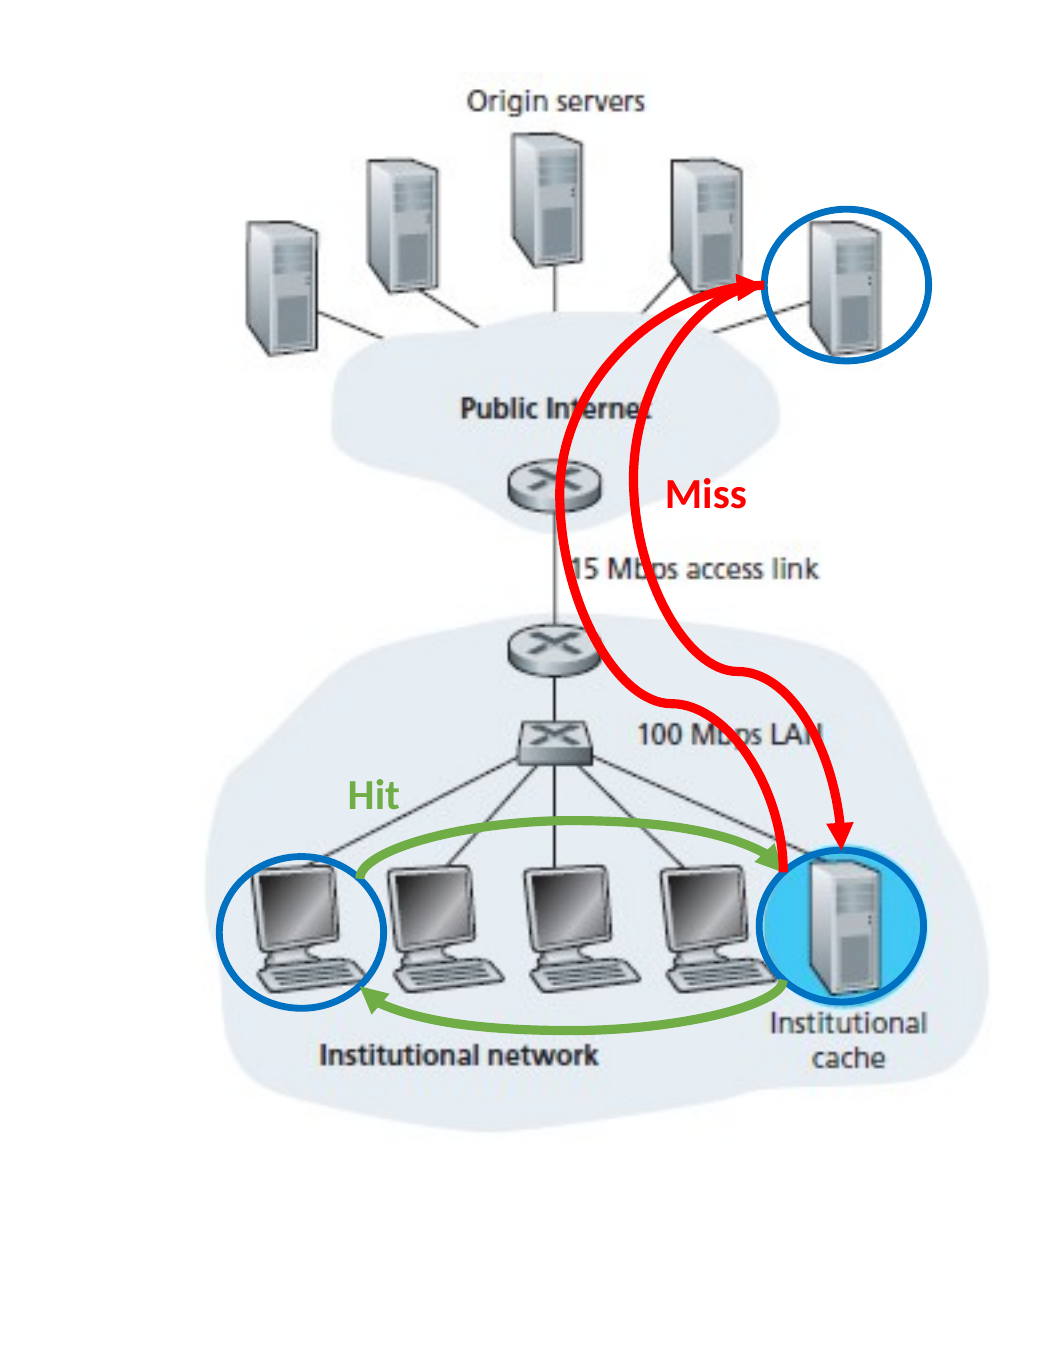
\includegraphics[width=0.9\linewidth]{cap05/cache_istituzionale.png}
\end{minipage}\hfill
\begin{minipage}{0.62\linewidth}
Le cache vengono spesso installate nella rete locale di un'azienda o di un ente.
\dfn{Hit, miss e hit rate}{
    Si ha un \textbf{hit} quando la cache fornisce un oggetto \textbf{senza contattare} il server di
    origine; un \textbf{miss} quando deve andarlo a prendere. La \textbf{hit rate} è la frazione di
    richieste soddisfatte dalla cache: tipicamente \textbf{tra 0{,}2 e 0{,}7}, e cresce con il numero di
    client che usano la cache.
}
Fino al 70\% delle richieste, quindi, può essere servito localmente.
\end{minipage}
\caption{Una cache istituzionale: il percorso rosso (miss) esce su Internet, quello verde (hit) resta nella rete locale.}
\end{figure}

\subsection{Il GET condizionale}

Il caching introduce un problema nuovo: la copia in cache potrebbe essere \textbf{vecchia}, se nel
frattempo l'oggetto è cambiato sul server.

\dfn{GET condizionale}{
    Un \textbf{GET condizionale} è una richiesta HTTP con metodo GET e header
    \texttt{If-Modified-Since}. Il server invia l'oggetto \textbf{solo se} è stato modificato dopo la data
    indicata; altrimenti risponde \texttt{304 Not Modified}, senza corpo.
}

\begin{figure}[H]
\centering
\begin{tikzpicture}[yscale=0.8, every node/.style={font=\scriptsize\sffamily}]
  \timeline{a}{0}{Host A}{9}
  \timeline{c}{5}{Cache}{9}
  \timeline{s}{10}{Server}{9}
  \draw[msg, netblue] (0,-0.4) -- node[above, sloped] {GET oggetto} (5,-1.0);
  \draw[msg, netblue] (5,-1.1) -- node[above, sloped] {GET oggetto} (10,-1.7);
  \draw[msg, netgreen] (10,-1.9) -- node[above, sloped] {200 OK, Last-Modified: X, oggetto} (5,-2.5);
  \node[draw, fill=llink!60, rounded corners, font=\scriptsize\sffamily] at (5,-2.95) {salva l'oggetto con data X};
  \draw[msg, netgreen] (5,-3.4) -- node[above, sloped] {200 OK, oggetto} (0,-4.0);
  \node[anchor=east, text=netred] at (-0.2,-4.9) {più tardi, Host B:};
  \draw[msg, netblue] (0,-5.0) -- node[above, sloped] {GET oggetto} (5,-5.6);
  \draw[msg, netred] (5,-5.8) -- node[above, sloped] {GET oggetto, If-Modified-Since: X} (10,-6.4);
  \draw[msg, netred] (10,-6.6) -- node[above, sloped] {304 Not Modified (nessun corpo)} (5,-7.2);
  \draw[msg, netgreen] (5,-7.5) -- node[above, sloped] {200 OK, oggetto (dalla cache)} (0,-8.1);
\end{tikzpicture}
\caption{La cache verifica con un GET condizionale che la propria copia sia ancora valida: se lo è, l'oggetto non viaggia di nuovo.}
\end{figure}

Se l'oggetto è aggiornato, alla cache basta una piccola risposta del server (niente oggetto da
ritrasmettere) e il client riceve la copia locale.

\subsection{Il caching nel browser}

Anche i \textbf{browser} fanno caching in locale, con lo stesso principio: conservano gli oggetti già
scaricati per non doverli richiedere al server. È una tecnica comunissima che migliora drasticamente
le prestazioni. La copia locale però può non essere aggiornata, e questo genera errori piuttosto
frequenti (la classica pagina che ``non si aggiorna'' finché non si svuota la cache).

\subsection{Oltre il caching: i proxy istituzionali}

\begin{figure}[H]
\centering
\begin{tikzpicture}[every node/.style={font=\footnotesize\sffamily}]
  \node (c) at (0,0) {\icon[1cm]{pc}}; \node[below=-2pt of c] {client};
  \node[netcloud, minimum width=4.2cm, minimum height=2.2cm] (inst) at (4.6,0) {};
  \node at (4.0,0.35) {rete istituzionale};
  \node (px) at (5.3,-0.3) {\icon[0.55cm]{server}}; \node[font=\scriptsize\sffamily] at (5.3,-0.95) {proxy};
  \node[netcloud, minimum width=2.6cm] (inet) at (9.2,0) {Internet};
  \node (o) at (12.1,0) {\icon[0.7cm]{server}}; \node[below=-1pt of o] {server di origine};
  \draw[msg, netblue] (c) -- (px);
  \draw[msg, netblue] (px) -- (inet); \draw[msg, netblue] (inet) -- (o);
  \node[text width=6cm, align=center, text=netred] at (8.2,-1.8) {per il server di origine la richiesta arriva dall'istituzione, non dal client};
\end{tikzpicture}
\caption{Un proxy istituzionale: le richieste escono a nome dell'ente.}
\end{figure}

Oltre alle prestazioni, i proxy servono ad \textbf{accedere a servizi istituzionali}. La rete
dell'Ateneo, per esempio, offre un proxy Web (\texttt{proxy.unina.it}): poiché le richieste vengono
inoltrate dal proxy, per il server di origine \textbf{arrivano tutte dall'istituzione}. Così, da casa, si
possono consultare riviste scientifiche abbonate dall'Università. Esistono anche molti proxy
commerciali o gratuiti su Internet.

% ══════════════════════════════════════════════════════════════
\section{Riepilogo}
% ══════════════════════════════════════════════════════════════

\riepilogo{
\begin{itemize}
    \item Richieste e risposte HTTP sono testo ASCII: \textbf{riga di richiesta/stato}, \textbf{header},
          \textbf{riga vuota}, \textbf{corpo}.
    \item Metodi principali: \textbf{GET}, \textbf{POST}, \textbf{HEAD}, \textbf{PUT}, \textbf{DELETE}.
    \item Codici di stato: 1xx informativi, 2xx successo, 3xx redirezione, 4xx errore del client, 5xx errore del server.
    \item I \textbf{cookie} (Set-cookie / Cookie + file sul client + database sul server) danno uno stato a un
          protocollo stateless, con implicazioni sulla privacy.
    \item Le \textbf{Web cache} (proxy) riducono tempi e traffico; il \textbf{GET condizionale}
          (\texttt{If-Modified-Since} / \texttt{304 Not Modified}) evita copie vecchie.
\end{itemize}
}
  % HTTP: messaggi, cookie, cache
  \chapter{Posta elettronica e applicazioni peer-to-peer}

% ══════════════════════════════════════════════════════════════
\section{La posta elettronica}
% ══════════════════════════════════════════════════════════════

La posta elettronica (\emph{e-mail}) è una delle applicazioni più antiche e importanti di Internet.
È realizzata in modo \textbf{client-server}, con due tipi di host:

\begin{itemize}
    \item lo \textbf{user agent}: l'applicazione con cui l'utente gestisce la posta (Thunderbird, K-9 Mail,
          l'app Mail del telefono, \dots);
    \item il \textbf{mail server}: un server che conserva la posta e mantiene una \textbf{casella}
          (\emph{mailbox}) per ciascun utente.
\end{itemize}

A differenza di HTTP, qui la comunicazione avviene \textbf{anche tra server}. Servono quindi due
applicazioni (e due protocolli): una tra user agent e mail server, e una tra mail server e mail server.

\begin{figure}[H]
\centering
\begin{tikzpicture}[every node/.style={font=\footnotesize\sffamily},
  ms/.style={draw=netblue, fill=cloudbg, rounded corners, minimum width=2.4cm, minimum height=1.5cm, align=center}]
  \node[ms] (s1) at (0,0) {\icon[0.5cm]{server}\\mail server\\di Alice};
  \node[ms] (s2) at (7,0) {\icon[0.5cm]{server}\\mail server\\di Bob};
  \node[ms] (s3) at (3.5,-2.6) {\icon[0.5cm]{server}\\altro\\mail server};
  \node (ua1) at (-3.4,1.2) {\icon[1cm]{laptop}}; \node[below=-2pt of ua1] {user agent (Alice)};
  \node (ua2) at (10.4,1.2) {\icon[0.7cm]{smartphone}}; \node[below=-2pt of ua2] {user agent (Bob)};
  \node (ua3) at (-3.4,-2.2) {\icon[0.9cm]{pc}}; \node[below=-2pt of ua3] {user agent};
  \draw[msg, netred, very thick] (ua1) -- node[above, sloped] {SMTP} (s1);
  \draw[msg, netred, very thick] (s1) -- node[above] {SMTP} (s2);
  \draw[msg, netgreen, very thick] (s2) -- node[above, sloped] {POP3 / IMAP / HTTP} (ua2);
  \draw[msg, netred, {Stealth}-{Stealth}] (s1) -- node[above, sloped] {SMTP} (s3);
  \draw[msg, netred, {Stealth}-{Stealth}] (s2) -- node[above, sloped] {SMTP} (s3);
  \draw[{Stealth}-{Stealth}, thick, netgreen] (ua3) -- (s3);
  \foreach \s in {s1, s2, s3} \draw[fill=llink] ([xshift=-0.35cm, yshift=-0.55cm]\s.south east) rectangle ++(0.3,0.25);
  \node[lbl] at (8.9,-1.2) {\colorbox{llink}{\strut}\ casella di Bob};
\end{tikzpicture}
\caption{Il sistema di posta: SMTP per inviare (dagli user agent ai server e tra server), protocolli di accesso per leggere la posta dalla propria casella.}
\end{figure}

Gli utenti non si scambiano la posta direttamente (come nella messaggistica istantanea): si
preferisce passare per i mail server, più affidabili e specializzati.

% ══════════════════════════════════════════════════════════════
\section{SMTP}
% ══════════════════════════════════════════════════════════════

\dfn{SMTP}{
    Il \textbf{Simple Mail Transfer Protocol} (SMTP) è il principale protocollo applicativo usato per
    \textbf{trasferire la posta tra mail server}. Ha un lato client (chi invia) e un lato server (chi
    riceve), entrambi eseguiti sui mail server, e usa il trasporto affidabile di \textbf{TCP} sulla
    \textbf{porta 25}.
}

Quando un nuovo messaggio arriva sul server, viene messo nella casella del destinatario, in attesa
che lo user agent lo scarichi.

\subsection{Il flusso completo di una mail}

Alice invia una mail a Bob (\texttt{bob@someschool.edu}). Sono coinvolti quattro elementi: lo user agent
di Alice, il mail server di Alice, il mail server di Bob, lo user agent di Bob.

\begin{figure}[H]
\centering
\begin{tikzpicture}[every node/.style={font=\footnotesize\sffamily}]
  \node (a) at (0,0) {\icon[1cm]{laptop}}; \node[below=-2pt of a] {user agent di Alice};
  \node[draw=netblue, fill=cloudbg, rounded corners, minimum width=2.6cm, minimum height=1.6cm] (sa) at (4,0) {};
  \node at (4,0.45) {mail server di Alice};
  \node[draw, fill=llink, minimum width=1.4cm, minimum height=0.4cm] at (4,-0.3) {coda messaggi};
  \node[draw=netblue, fill=cloudbg, rounded corners, minimum width=2.6cm, minimum height=1.6cm] (sb) at (9.5,0) {};
  \node at (9.5,0.45) {mail server di Bob};
  \node[draw, fill=llink, minimum width=1.4cm, minimum height=0.4cm] at (9.5,-0.3) {casella di Bob};
  \node (b) at (13.5,0) {\icon[0.7cm]{smartphone}}; \node[below=-2pt of b] {user agent di Bob};
  \draw[msg, very thick] (a) -- node[above] {\circled{2}} (sa);
  \draw[msg, very thick, netred] (sa) -- node[above] {\circled{3}\ \circled{4}\ SMTP su TCP} (sb);
  \draw[msg, very thick, netgreen] (sb) -- node[above] {\circled{6}} (b);
  \node[above=6pt of a] {\circled{1}};
  \node[above=-2pt of sb.north] {\circled{5}};
\end{tikzpicture}
\caption{I sei passi dell'invio di una mail da Alice a Bob.}
\end{figure}

\begin{enumerate}
    \item Alice apre il suo user agent, inserisce l'indirizzo di Bob, scrive il messaggio e chiede di inviarlo.
    \item Lo user agent di Alice invia il messaggio al \textbf{suo} mail server, dove viene messo in una
          \textbf{coda di messaggi}.
    \item Il lato client di SMTP, sul server di Alice, vede il messaggio in coda e \textbf{apre una connessione
          TCP} verso il server SMTP in esecuzione sul mail server di Bob.
    \item Dopo un handshaking SMTP iniziale, il client SMTP invia il messaggio di Alice sulla connessione TCP.
    \item Sul server di Bob il lato server di SMTP riceve il messaggio e lo mette nella \textbf{casella di Bob}.
    \item Bob apre il proprio user agent e legge il messaggio quando vuole.
\end{enumerate}

\info{Nessun server intermedio}{
    SMTP di norma \textbf{non} usa mail server intermedi: la connessione TCP va direttamente dal server di
    Alice a quello di Bob, anche se sono ai lati opposti del pianeta. Se il server di Bob è spento, il
    messaggio resta nella coda del server di Alice, che riprova più tardi.
}

\subsection{Dettagli del protocollo}

\begin{itemize}
    \item Il client SMTP (sul server mittente) apre una connessione TCP verso la \textbf{porta 25} del server
          SMTP (sul server destinatario).
    \item Se il server non risponde, il client \textbf{riprova più tardi}.
    \item Stabilita la connessione, client e server fanno un \textbf{handshaking applicativo}: si presentano
          prima di trasferire informazioni. In questa fase il client indica l'indirizzo del \textbf{mittente} e
          quello del \textbf{destinatario}.
    \item Poi il client invia il messaggio, contando sul trasferimento affidabile di TCP per farlo arrivare
          senza errori.
\end{itemize}

\begin{esempio}{Un dialogo SMTP}
Le righe che iniziano con \texttt{S:} sono inviate dal server, quelle con \texttt{C:} dal client
(da Kurose). Come HTTP, anche SMTP usa comandi testuali leggibili.
\begin{lstlisting}
S: 220 hamburger.edu
C: HELO crepes.fr
S: 250 Hello crepes.fr, pleased to meet you
C: MAIL FROM: <alice@crepes.fr>
S: 250 alice@crepes.fr ... Sender ok
C: RCPT TO: <bob@hamburger.edu>
S: 250 bob@hamburger.edu ... Recipient ok
C: DATA
S: 354 Enter mail, end with "." on a line by itself
C: Do you like ketchup?
C: How about pickles?
C: .
S: 250 Message accepted for delivery
C: QUIT
S: 221 hamburger.edu closing connection
\end{lstlisting}
\end{esempio}

% ══════════════════════════════════════════════════════════════
\section{Accedere alla posta}
% ══════════════════════════════════════════════════════════════

Usare dei server SMTP è più affidabile della consegna diretta da utente a utente:

\begin{itemize}
    \item i server sono, per definizione, \textbf{sempre accesi} e visibili a tutti i dispositivi della rete
          (il portatile di Bob, invece, può essere spento);
    \item i server sono \textbf{certificati};
    \item il server può \textbf{riprovare continuamente} a consegnare la posta se la consegna fallisce, un
          processo piuttosto oneroso da fare sul proprio dispositivo.
\end{itemize}

D'altra parte, per \textbf{leggere} la posta dal proprio server serve un'altra applicazione
client-server, con un protocollo diverso da SMTP (SMTP è un protocollo ``push'': serve a spingere la
posta verso un server, non a tirarla giù). I più diffusi sono POP3, IMAP e HTTP.

\subsection{POP3}

\dfn{POP3}{
    Il \textbf{Post Office Protocol --- Version 3} (POP3) è un protocollo di accesso alla posta
    estremamente semplice. Lo user agent (client) apre una connessione TCP verso il mail server sulla
    \textbf{porta 110}.
}

Stabilita la connessione, POP3 attraversa tre fasi:

\begin{figure}[H]
\centering
\begin{tikzpicture}[every node/.style={font=\footnotesize\sffamily}, ph/.style={draw, rounded corners, fill=#1, minimum width=3.6cm, minimum height=1.6cm, align=center, text width=3.4cm}]
  \node[ph=lapp!60] (a) at (0,0) {\textbf{1. Autorizzazione}\\[2pt] \scriptsize invio di nome utente e password};
  \node[ph=ltra!60] (t) at (4.8,0) {\textbf{2. Transazione}\\[2pt] \scriptsize scaricare messaggi, marcarli per la cancellazione, statistiche};
  \node[ph=lnet!60] (u) at (9.6,0) {\textbf{3. Aggiornamento}\\[2pt] \scriptsize dopo \texttt{quit}: il server cancella i messaggi marcati};
  \draw[msg, very thick] (a) -- (t); \draw[msg, very thick] (t) -- (u);
\end{tikzpicture}
\caption{Le tre fasi di una sessione POP3.}
\end{figure}

\begin{enumerate}
    \item \textbf{Autorizzazione}: lo user agent invia nome utente e password per autenticare l'utente.
    \item \textbf{Transazione}: lo user agent può recuperare messaggi, marcarli per la cancellazione, togliere
          le marcature e ottenere statistiche sulla casella.
    \item \textbf{Aggiornamento}: quando il client dà il comando \texttt{quit}, la sessione termina e il server
          cancella i messaggi marcati.
\end{enumerate}

\subsection{IMAP}

Con POP3 i messaggi si possono solo scaricare o cancellare: cercare, organizzare in cartelle e simili va
fatto sulla macchina locale. Se si legge la posta da più dispositivi, questo è un problema.

\dfn{IMAP}{
    L'\textbf{Internet Mail Access Protocol} (IMAP, porta 143) permette al server di offrire funzioni
    aggiuntive, mantenendo la posta \textbf{sul server}:
    \begin{itemize}
      \item creare e gestire \textbf{cartelle} sul server;
      \item \textbf{cercare} nelle cartelle remote i messaggi che soddisfano certi criteri;
      \item scaricare solo \textbf{parti} di un messaggio (solo le intestazioni, solo gli allegati, \dots);
      \item collegare \textbf{più client} contemporaneamente alla stessa casella.
    \end{itemize}
}

\subsection{HTTP (webmail)}

Sempre più utenti inviano e leggono la posta dal \textbf{browser}. L'accesso via Web fu introdotto da
Hotmail a metà degli anni '90 ed è oggi l'approccio più diffuso (Google, Yahoo!, Libero, e quasi tutte le
università e le aziende, UniNA compresa). In questo caso lo user agent è un normale browser, e l'utente
comunica con la propria casella remota via \textbf{HTTP} invece che con POP3 o IMAP.

\warning{Tra server resta SMTP}{
    HTTP sostituisce POP3/IMAP solo tra \textbf{user agent e server}. Tra \textbf{mail server} la posta
    continua a viaggiare con SMTP.
}

\begin{table}[H]
\centering
\begin{tabular}{llll}
\toprule
\textbf{Protocollo} & \textbf{Tra} & \textbf{Porta TCP} & \textbf{Caratteristica} \\
\midrule
SMTP & server $\leftrightarrow$ server, user agent $\rightarrow$ server & 25 & invio (push) \\
POP3 & user agent $\leftarrow$ server & 110 & scarica e (di solito) cancella \\
IMAP & user agent $\leftrightarrow$ server & 143 & la posta resta sul server, cartelle, ricerca \\
HTTP & browser $\leftrightarrow$ server & 80/443 & webmail \\
\bottomrule
\end{tabular}
\caption{I protocolli della posta elettronica.}
\end{table}

% ══════════════════════════════════════════════════════════════
\section{Peer-to-peer}
% ══════════════════════════════════════════════════════════════

A differenza del client-server, un'architettura P2P usa i server in modo minimo, o per nulla: coppie di
host collegati in modo intermittente (i \textbf{peer}) comunicano direttamente. I peer non appartengono
a un fornitore di servizi: sono computer e portatili controllati dagli utenti.

\subsection{Distribuire un file: due modi}

Un file, un server, e molti host che ne vogliono una copia.

\begin{figure}[H]
\centering
\begin{tikzpicture}[every node/.style={font=\footnotesize\sffamily}]
  \begin{scope}
    \node[font=\small\bfseries\sffamily] at (0,2.4) {Client-server};
    \node (srv) at (0,1.4) {\icon[0.7cm]{server}};
    \node[right=1pt of srv, text=netred] {server: carica a $u_s$};
    \foreach \x [count=\i] in {-2.4,-1.2,0,1.2,2.4} {
      \node (c\i) at (\x,-0.8) {\icon[0.65cm]{laptop}};
      \draw[-{Stealth}, thick, netred] (srv) -- node[fill=white, inner sep=0.5pt, font=\scriptsize\sffamily] {$F$} (c\i);
    }
    \node[lbl, text width=5.2cm] at (0,-2.0) {il server invia \textbf{$N$ copie} complete: $N F$ bit, tutti con la sua sola banda};
  \end{scope}
  \begin{scope}[xshift=8cm]
    \node[font=\small\bfseries\sffamily] at (0,2.4) {Peer-to-peer};
    \node (srv) at (0,1.4) {\icon[0.7cm]{server}};
    \node[right=1pt of srv, text=netred] {server};
    \foreach \x/\y [count=\i] in {-2.7/-1.0, -1.5/0.35, 0/-0.45, 1.5/0.35, 2.7/-1.0} {
      \node (p\i) at (\x,\y) {\icon[0.6cm]{laptop}};
    }
    \draw[-{Stealth}, thick, netred, shorten >=2pt] (srv) -- node[right, font=\scriptsize\sffamily] {$\approx F$} (p3);
    \foreach \a/\b in {3/2, 3/4, 2/1, 4/5} \draw[-{Stealth}, thick, netgreen!60!black, shorten >=3pt, shorten <=3pt] (p\a) -- (p\b);
    \draw[-{Stealth}, thick, netgreen!60!black, shorten >=3pt, shorten <=3pt] (p1) to[bend right=25] (p3);
    \draw[-{Stealth}, thick, netgreen!60!black, shorten >=3pt, shorten <=3pt] (p5) to[bend left=25] (p3);
    \node[lbl, text width=5.2cm] at (0,-2.0) {il server invia \textbf{circa una copia}; i peer si passano i pezzi, ciascuno con la propria banda di upload $u_i$};
  \end{scope}
\end{tikzpicture}
\caption{A sinistra il server invia $N$ copie; a destra ne invia circa una, e i peer si scambiano i pezzi tra loro.}
\end{figure}

Il ragionamento si può rendere quantitativo. Un file di $F$ bit va distribuito a $N$ peer; il server carica a
velocità $u_s$, il peer $i$ carica a $u_i$, e $d_{\min}$ è la velocità di download del peer più lento.

\dfn{Tempo minimo di distribuzione}{
    $$D_{\text{cs}} = \max\left\{\frac{N F}{u_s},\ \frac{F}{d_{\min}}\right\} \qquad\qquad
      D_{\text{P2P}} = \max\left\{\frac{F}{u_s},\ \frac{F}{d_{\min}},\ \frac{N F}{u_s + \sum_{i=1}^{N} u_i}\right\}$$
}

\begin{itemize}
    \item \textbf{Client-server}: il server da solo deve inviare $N F$ bit alla velocità $u_s$, e nessun client può
          finire prima di aver scaricato $F$ bit alla propria velocità (il più lento a $d_{\min}$). Il tempo
          \textbf{cresce linearmente} con $N$, senza limite.
    \item \textbf{P2P}: il server deve inviare almeno una copia ($F/u_s$); il peer più lento non può scaricare più
          in fretta di $F/d_{\min}$; e i $N F$ bit complessivi vengono caricati usando la banda del server
          \textbf{più quella di tutti i peer}. Ogni nuovo peer aggiunge un $F$ al numeratore, ma anche il suo $u_i$
          al denominatore.
\end{itemize}

\begin{figure}[H]
\centering
\begin{tikzpicture}
  \begin{axis}[width=9cm, height=5.4cm, xlabel={numero di peer $N$}, ylabel={tempo minimo (ore)},
      xmin=0, xmax=35, ymin=0, ymax=3.6, legend pos=north west, legend style={font=\scriptsize\sffamily},
      tick label style={font=\scriptsize}, label style={font=\footnotesize\sffamily}, grid=major, grid style={gray!20}]
    \addplot[very thick, netred, domain=0:35, samples=50] {x/10};
    \addlegendentry{client-server}
    \addplot[very thick, netblue, domain=0:35, samples=80] {max(0.1, x/(10+x))};
    \addlegendentry{P2P}
  \end{axis}
\end{tikzpicture}
\caption{Tempo minimo di distribuzione con $u_s = 10u$ (tutti i peer caricano a $u$), $F/u = 1$ ora e $d_{\min}$ abbondante (da Kurose): il client-server cresce come $N/10$, il P2P come $N/(10+N)$ e non supera mai 1 ora.}
\end{figure}

Mille volte i peer sono mille volte l'attesa nel client-server, e quasi nessuna attesa in più nel P2P: è la
\textbf{auto-scalabilità} del P2P, e un esercizio numerico completo si trova nella parte degli esercizi.

\info{Pro e contro del P2P}{
    Nella condivisione di file il P2P \textbf{scala} di solito molto meglio del client-server. D'altra parte è
    più \textbf{complesso da implementare}, e avere tanti client in comunicazione diretta tra loro pone
    problemi di \textbf{sicurezza}.
}

% ══════════════════════════════════════════════════════════════
\section{BitTorrent}
% ══════════════════════════════════════════════════════════════

Un protocollo P2P molto diffuso per la distribuzione di file è \textbf{BitTorrent} (circa 150--170
milioni di utenti stimati nel 2023).

\dfn{Torrent e chunk}{
    Un \textbf{torrent} è l'insieme di tutti i peer che partecipano alla distribuzione di un certo file.
    I peer di un torrent si scambiano \textbf{chunk}, pezzi del file di uguale dimensione
    (tipicamente 256~kB).
}

\subsection{Il ciclo di vita di un peer}

Quando un peer entra in un torrent, senza avere ancora alcun chunk:

\begin{itemize}
    \item comincia ad \textbf{accumulare chunk};
    \item mentre scarica, \textbf{carica} anche chunk verso altri peer;
    \item quando ha l'intero file può andarsene (egoisticamente) oppure restare (altruisticamente) a
          continuare a caricare chunk per gli altri.
\end{itemize}

I peer possono lasciare il torrent in qualsiasi momento, anche con solo una parte dei chunk, e
rientrare più tardi.

\subsection{Il tracker}

\dfn{Tracker}{
    Ogni torrent ha un nodo di infrastruttura, il \textbf{tracker}, che tiene traccia dei peer che
    partecipano al torrent. È, in sostanza, un \textbf{server}, in un'architettura che avrebbe dovuto farne a meno:
    un altro esempio di architettura ibrida.
}

\begin{figure}[H]
\centering
\begin{tikzpicture}[every node/.style={font=\footnotesize\sffamily}]
  \node (tr) at (0,2.8) {\icon[0.7cm]{server}}; \node[right=2pt of tr, text=netred] {tracker};
  \node[ellipse, minimum width=9.5cm, minimum height=3.8cm, fill=netgreen!8, draw=netgreen!60, thick] at (0.4,-0.6) {};
  \node[text=netgreen!50!black, font=\small\bfseries\sffamily] at (-3.2,0.9) {torrent};
  \node (alice) at (-6.2,0) {\icon[1cm]{laptop}}; \node[below=-2pt of alice, text=netblue] {nuovo peer (Alice)};
  \foreach \x/\y/\ic [count=\i] in {-2.2/0.3/pc, 0/0.6/laptop, 2.4/0.2/pc, -1.2/-1.6/laptop, 1.3/-1.7/pc, 3.3/-1.1/laptop} {
    \node (p\i) at (\x,\y) {\icon[0.6cm]{\ic}};
  }
  \draw[msg, dashed, netred] (alice) to[bend left=20] node[above, sloped] {1. registrazione} (tr);
  \draw[msg, dashed, netred] (tr) to[bend left=10] node[below, sloped] {2. lista di peer} (alice);
  \foreach \i in {1,4,2} \draw[{Stealth}-{Stealth}, thick, netblue] (alice) -- (p\i);
  \node[text=netblue] at (-4.2,-1.8) {3. connessioni TCP};
  \foreach \a/\b in {1/2, 2/3, 3/6, 4/5, 5/6, 1/4, 2/5} \draw[thick, black!35] (p\a) -- (p\b);
  \foreach \i/\c in {1/lapp, 2/ltra, 3/lnet} \fill[\c] (5.2+\i*0.35,2.4) rectangle ++(0.3,0.3);
  \node[right] at (6.4,2.55) {chunk del file};
\end{tikzpicture}
\caption{Un nuovo peer si registra presso il tracker, riceve un sottoinsieme di peer e apre con loro connessioni TCP.}
\end{figure}

Quando un nuovo peer entra in un torrent:

\begin{itemize}
    \item si \textbf{registra} presso il tracker e lo informa periodicamente del proprio stato;
    \item il tracker gli fornisce gli indirizzi IP di un \textbf{sottoinsieme casuale} di peer del torrent;
    \item avuta la lista, il nuovo peer prova ad aprire \textbf{connessioni TCP} concorrenti con tutti i peer
          della lista, che diventano i suoi \textbf{vicini} (\emph{neighbors});
    \item durante l'esecuzione alcuni vicini se ne vanno, mentre altri peer (fuori dalla lista iniziale)
          possono chiedere di connettersi.
\end{itemize}

In ogni istante ogni peer ha un sottoinsieme diverso dei chunk. Periodicamente un peer chiede a ogni
vicino (sulle connessioni TCP) la lista dei chunk che possiede.

\subsection{Le politiche del client}

\dfn{Rarest first}{
    Chi \textbf{scarica} decide quali chunk chiedere, e a chi, secondo il principio \textbf{rarest first}:
    si danno priorità ai chunk che hanno \textbf{meno copie} tra i vicini. Così i chunk rari vengono
    ridistribuiti più rapidamente e il numero di copie di ciascun chunk nel torrent tende a equilibrarsi.
}

Chi \textbf{carica} decide a quali richieste rispondere secondo due principi intrecciati:

\begin{itemize}
    \item \textbf{Scambio} (\emph{trading}, detto anche \emph{tit-for-tat}): si dà priorità ai
          \textbf{4 vicini migliori}, cioè quelli che in quel momento ci stanno inviando dati alla velocità più
          alta. Il controllo viene ripetuto ogni \textbf{10 secondi} e la lista dei 4 migliori aggiornata.
    \item \textbf{Selezione casuale} (\emph{optimistic unchoking}): ogni \textbf{30 secondi} si sceglie anche un
          vicino \textbf{a caso} e gli si inviano chunk. Se lo scambio va bene (i due sono buoni partner), i due
          entrano nelle rispettive liste dei migliori. Questo permette anche ai peer con velocità di upload
          compatibili di trovarsi, e ai nuovi arrivati di ricevere i primi chunk.
\end{itemize}

\begin{esempio}{Perché la selezione casuale}
Alice ha appena iniziato e non ha nulla da offrire: nessuno la metterebbe tra i propri 4 migliori. Grazie
alla selezione casuale, prima o poi un peer (Bob) le invia qualche chunk; Alice diventa così capace di
ricambiare, magari entra tra i migliori di Bob, e Bob tra i suoi. Chi carica di più riceve di più: i
``parassiti'' che scaricano senza caricare vengono penalizzati.
\end{esempio}

% ══════════════════════════════════════════════════════════════
\section{Riepilogo}
% ══════════════════════════════════════════════════════════════

\riepilogo{
\begin{itemize}
    \item La posta usa \textbf{user agent} e \textbf{mail server}; \textbf{SMTP} (TCP, porta 25) trasferisce i
          messaggi fino alla casella del destinatario, anche tra server.
    \item Per leggere la posta servono protocolli di accesso: \textbf{POP3} (semplice: autorizzazione,
          transazione, aggiornamento), \textbf{IMAP} (cartelle e ricerca sul server), \textbf{HTTP} (webmail).
    \item Nel \textbf{P2P} i peer sono client e server insieme: la distribuzione di file scala meglio.
    \item \textbf{BitTorrent}: torrent, chunk, \textbf{tracker}; \textbf{rarest first} per scaricare,
          \textbf{4 migliori ogni 10 s} + \textbf{uno casuale ogni 30 s} per caricare.
\end{itemize}
}
  % Posta elettronica e P2P
  \chapter{Il DNS}

% ══════════════════════════════════════════════════════════════
\section{Il problema: nomi e indirizzi}
% ══════════════════════════════════════════════════════════════

Un host si può identificare in due modi: con un \textbf{nome} (\emph{hostname}) o con un
\textbf{indirizzo IP}. Le persone preferiscono i nomi, facili da ricordare; i dispositivi di rete
preferiscono gli indirizzi IP, di lunghezza fissa e strutturati gerarchicamente.

\begin{center}
\begin{tikzpicture}[every node/.style={font=\sffamily}]
  \node[draw, rounded corners, fill=lapp!40, minimum width=3.2cm, minimum height=0.9cm] (n) at (0,0) {\texttt{www.unina.it}};
  \node[draw, rounded corners, fill=lnet!40, minimum width=3.2cm, minimum height=0.9cm] (i) at (8,0) {\texttt{143.225.15.50}};
  \draw[msg, very thick, primary] (n) -- node[above, font=\small\bfseries\sffamily] {DNS} node[below, font=\scriptsize\sffamily] {traduzione} (i);
  \node[below=2pt of n, font=\scriptsize\sffamily] {comodo per le persone};
  \node[below=2pt of i, font=\scriptsize\sffamily] {comodo per i router};
\end{tikzpicture}
\end{center}

\dfn{Domain Name System (DNS)}{
    Il \textbf{DNS} è un protocollo di livello applicativo che gestisce la \textbf{traduzione dei nomi
    degli host in indirizzi IP}. È un protocollo \textbf{client-server}: un client DNS chiede a un server DNS
    la traduzione di un certo nome. I server DNS sono spesso macchine UNIX con il software \textbf{BIND}
    (\emph{Berkeley Internet Name Domain}) e usano tipicamente \textbf{UDP} sulla \textbf{porta 53}.
}

Il DNS è anche un esempio perfetto di \textbf{database distribuito}: nessun server contiene tutte le
associazioni, ma l'insieme dei server sì.

\info{Un'applicazione al servizio di altre applicazioni}{
    Il DNS non è quasi mai usato direttamente dagli utenti: lo usano le altre applicazioni. Quando il browser
    deve aprire \texttt{http://www.unina.it/index.html}, prima chiede al DNS l'indirizzo di
    \texttt{www.unina.it}, poi apre la connessione TCP verso quell'indirizzo. Il ritardo introdotto dal DNS
    si somma quindi a quello di ogni navigazione, ed è uno dei motivi per cui usa UDP e fa largo uso di cache.
}

\subsection{Perché non un repository centralizzato}

La soluzione più semplice sarebbe un unico server con una grande tabella nome--indirizzo. Non funziona:

\begin{itemize}
    \item \textbf{troppi host}: un'unica tabella con i nomi di tutta Internet sarebbe enorme e sempre da aggiornare;
    \item \textbf{distanza e ritardi}: un server unico sarebbe lontano dalla maggior parte degli utenti;
    \item \textbf{volume di traffico}: dovrebbe rispondere a tutte le interrogazioni del mondo;
    \item \textbf{single point of failure}: se si guasta, si ferma Internet.
\end{itemize}

Il DNS è quindi un sistema \textbf{distribuito} e \textbf{decentralizzato}:

\begin{itemize}
    \item \textbf{gerarchico};
    \item \textbf{basato sui domini};
    \item realizzato tramite un \textbf{database distribuito} su molti server.
\end{itemize}

\dfn{Resolver}{
    Il \textbf{resolver} è il programma (di solito una funzione di libreria) che restituisce l'indirizzo IP
    associato a un nome. Interroga un \textbf{server DNS locale}, e tutti i messaggi sono pacchetti
    \textbf{UDP}.
}

% ══════════════════════════════════════════════════════════════
\section{Lo spazio dei nomi DNS}
% ══════════════════════════════════════════════════════════════

\begin{itemize}
    \item La gerarchia dei nomi è organizzata dall'\textbf{ICANN} (\emph{Internet Corporation for Assigned
          Names and Numbers}).
    \item Sotto la radice ci sono i \textbf{domini di primo livello} (\emph{top-level domain}, TLD), alcune
          centinaia.
    \item Ogni dominio è diviso in \textbf{sottodomini}, e così via.
\end{itemize}

I domini di primo livello sono di due tipi, tutti gestiti da \emph{registrar} nominati dall'ICANN:

\begin{itemize}
    \item \textbf{generici}: \texttt{com}, \texttt{edu}, \texttt{org}, \texttt{net}, \texttt{aero}, \dots;
    \item \textbf{nazionali} (\emph{country code}): \texttt{it}, \texttt{uk}, \texttt{jp}, \texttt{tv}, \dots
\end{itemize}

\begin{figure}[H]
    \centering
    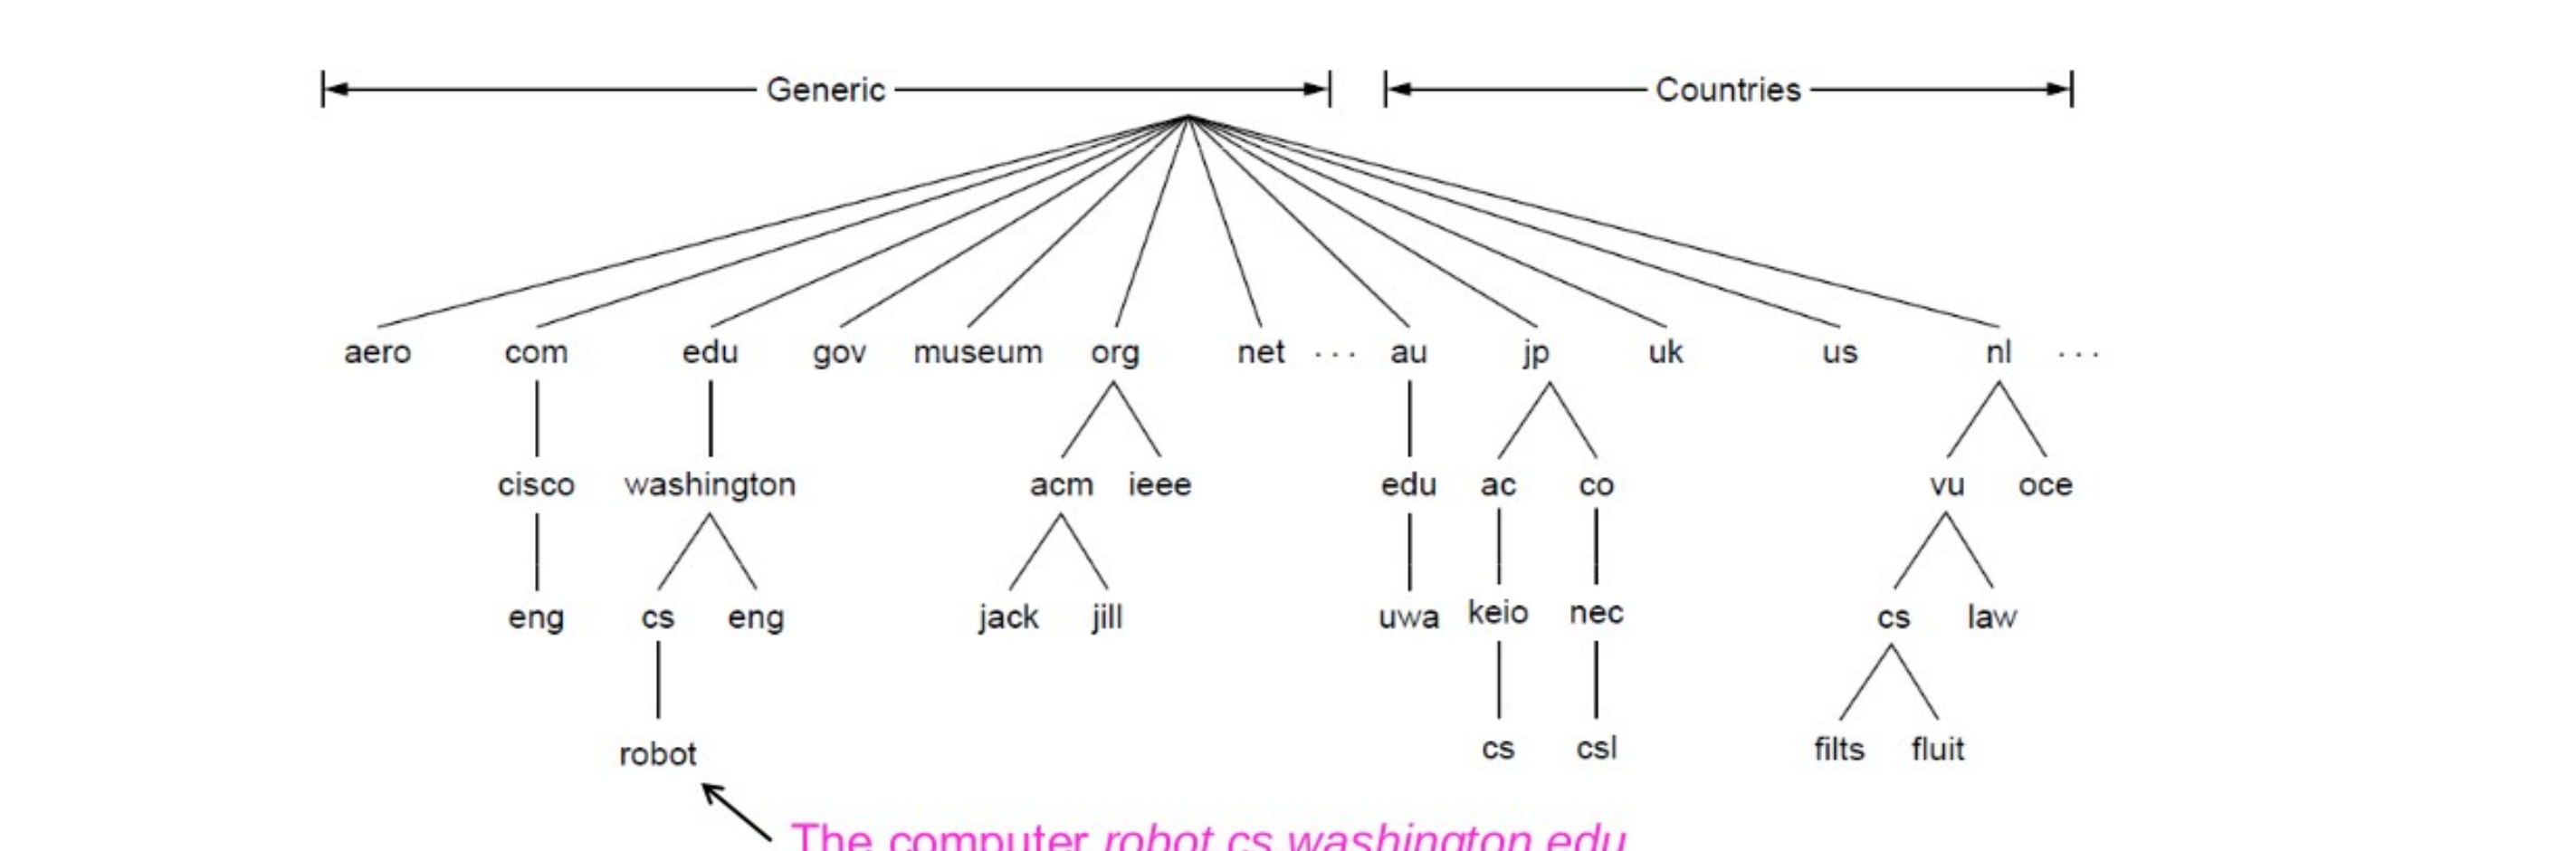
\includegraphics[width=0.85\linewidth]{cap07/albero_dns.png}
    \caption{Lo spazio dei nomi è un albero, dalla radice verso il basso; parti diverse sono delegate a organizzazioni diverse. In rosso il computer \texttt{robot.cs.washington.edu}.}
\end{figure}

\begin{table}[H]
\centering
\begin{tabular}{llcc}
\toprule
\textbf{Dominio} & \textbf{Uso previsto} & \textbf{Dal} & \textbf{Riservato?} \\
\midrule
com & commerciale & 1985 & no \\
edu & istituzioni educative & 1985 & sì \\
gov & governo & 1985 & sì \\
int & organizzazioni internazionali & 1988 & sì \\
mil & militare & 1985 & sì \\
net & fornitori di rete & 1985 & no \\
org & organizzazioni non profit & 1985 & no \\
aero, biz, info, name, pro, \dots & settori specifici & 2001--2010 & vari \\
\bottomrule
\end{tabular}
\caption{Alcuni domini generici di primo livello, controllati dall'ICANN.}
\end{table}

\subsection{I nomi di dominio}

\begin{figure}[H]
\centering
\begin{tikzpicture}[every node/.style={font=\footnotesize\sffamily}, dn/.style={draw, ellipse, fill=cloudbg, inner sep=2pt}]
  \node[dn, fill=lphy] (r) at (0,0) {radice};
  \node[dn] (edu) at (-3,-1.2) {edu}; \node[dn] (it) at (3,-1.2) {it};
  \node[dn] (mit) at (-3,-2.4) {mit}; \node[dn] (unina) at (3,-2.4) {unina};
  \node[dn] (eng) at (-3,-3.6) {eng}; \node[dn] (www) at (3,-3.6) {www};
  \draw (r) -- (edu) -- (mit) -- (eng); \draw (r) -- (it) -- (unina) -- (www);
  \draw[-{Stealth}, very thick, netred] (-2.2,-3.6) -- (-2.2,-1.2) -- (-0.7,-0.2);
  \node[anchor=west, text=netred, text width=4cm, align=left] at (-2,-2.7) {si legge \textbf{risalendo}\\ verso la radice:\\ \texttt{eng.mit.edu}};
  \node[anchor=west, text width=4cm, align=left] at (4,-3.6) {\texttt{www.unina.it.}\\\scriptsize (con il punto finale: nome assoluto)};
\end{tikzpicture}
\caption{Un nome di dominio è il percorso dal nodo verso la radice.}
\end{figure}

\begin{itemize}
    \item I nomi sono \textbf{percorsi verso l'alto}, dal dominio alla radice: \texttt{eng.mit.edu}.
    \item I percorsi \textbf{assoluti} terminano con un punto (\texttt{eng.mit.edu.}); quelli
          \textbf{relativi} vanno interpretati rispetto a un dominio di partenza.
    \item Si può registrare lo stesso nome sotto più TLD (\texttt{ibm.com}, \texttt{ibm.us}).
    \item Il \textbf{cyber-squatting} è la pratica di comprare domini solo per rivenderli poi alle aziende interessate.
    \item Ogni dominio \textbf{controlla l'assegnazione} dei domini sotto di lui; creare un nuovo dominio richiede
          il \textbf{permesso del dominio padre}.
    \item La struttura dei nomi \textbf{non} segue confini fisici o geografici (\texttt{cs.washington.edu} e un
          server in un altro continente possono stare nello stesso dominio).
\end{itemize}

% ══════════════════════════════════════════════════════════════
\section{I resource record}
% ══════════════════════════════════════════════════════════════

Il database distribuito del DNS è fatto di \textbf{resource record} (RR). Ogni record ha cinque campi:

\begin{center}
\begin{tikzpicture}[every node/.style={font=\small\sffamily}]
  \foreach \t/\c [count=\i] in {NAME/lapp, TTL/ltra, CLASS/lnet, TYPE/llink, VALUE (RDATA)/lphy}
    \node[field, fill=\c, minimum width=2.6cm, minimum height=0.8cm] at (\i*2.6,0) {\t};
\end{tikzpicture}
\end{center}

\begin{itemize}
    \item \textbf{NAME} (nome di dominio): il dominio a cui si riferisce il record. È la \textbf{chiave di
          ricerca} principale delle interrogazioni; di solito per ogni dominio esistono più record, su server diversi.
    \item \textbf{TTL} (\emph{time to live}): la durata di validità del record, in secondi. Lunga per host stabili
          (86\,400 = un giorno), breve per quelli volatili (60 = un minuto); il valore massimo è $2^{31}-1$ secondi,
          circa 68 anni.
    \item \textbf{CLASS}: per i record di Internet è sempre \textbf{IN}; gli altri codici sono usati raramente.
    \item \textbf{TYPE}: il tipo di record (tabella seguente).
    \item \textbf{VALUE} (RDATA): il valore, che dipende dal tipo: un dominio, un numero o una stringa ASCII.
\end{itemize}

\begin{table}[H]
\centering
\begin{tabular}{lll}
\toprule
\textbf{Tipo} & \textbf{Significato} & \textbf{Valore} \\
\midrule
SOA & \emph{Start Of Authority} & parametri della zona: server principale, contatto dell'amministratore, \dots \\
A & \emph{Address} & indirizzo IPv4 (32 bit) di un'interfaccia dell'host \\
AAAA & indirizzo IPv6 & indirizzo IPv6 (128 bit) \\
MX & \emph{Mail eXchange} & nome dell'host che accetta la posta per il dominio (con priorità) \\
NS & \emph{Name Server} & nome di un server DNS per il dominio \\
CNAME & \emph{Canonical NAME} & nome canonico di cui questo nome è un alias \\
PTR & \emph{Pointer} & nome associato a un indirizzo (ricerca inversa) \\
SPF & \emph{Sender Policy Framework} & regole su chi può inviare posta per il dominio \\
SRV & \emph{Service} & host che offre un certo servizio \\
TXT & \emph{Text} & testo ASCII descrittivo \\
\bottomrule
\end{tabular}
\caption{I tipi principali di resource record.}
\end{table}

\warning{Come ``leggere'' i record}{
    \begin{itemize}
      \item \texttt{(unina.it, dns.unina.it, IN, NS)}: \texttt{dns.unina.it} è un name server per il dominio \texttt{unina.it};
            la ricerca prosegue interrogando lui.
      \item \texttt{(www.unina.it, 143.225.15.50, IN, A)}: l'indirizzo IPv4 di \texttt{www.unina.it}.
      \item \texttt{(www.ibm.com, servereast.backup2.ibm.com, IN, CNAME)}: \texttt{www.ibm.com} è un alias;
            la ricerca \textbf{prosegue} con il nome canonico.
      \item \texttt{(ibm.com, mail.bar.ibm.com, IN, MX)}: la posta per \texttt{@ibm.com} va consegnata a \texttt{mail.bar.ibm.com}.
      \item Con PTR, invece, la ricerca \textbf{non prosegue}: si restituisce semplicemente il nome.
    \end{itemize}
    Un host può avere \textbf{più interfacce}, e quindi più record A.
}

\begin{esempio}{I record di un dominio: \texttt{cs.vu.nl}}
\begin{center}
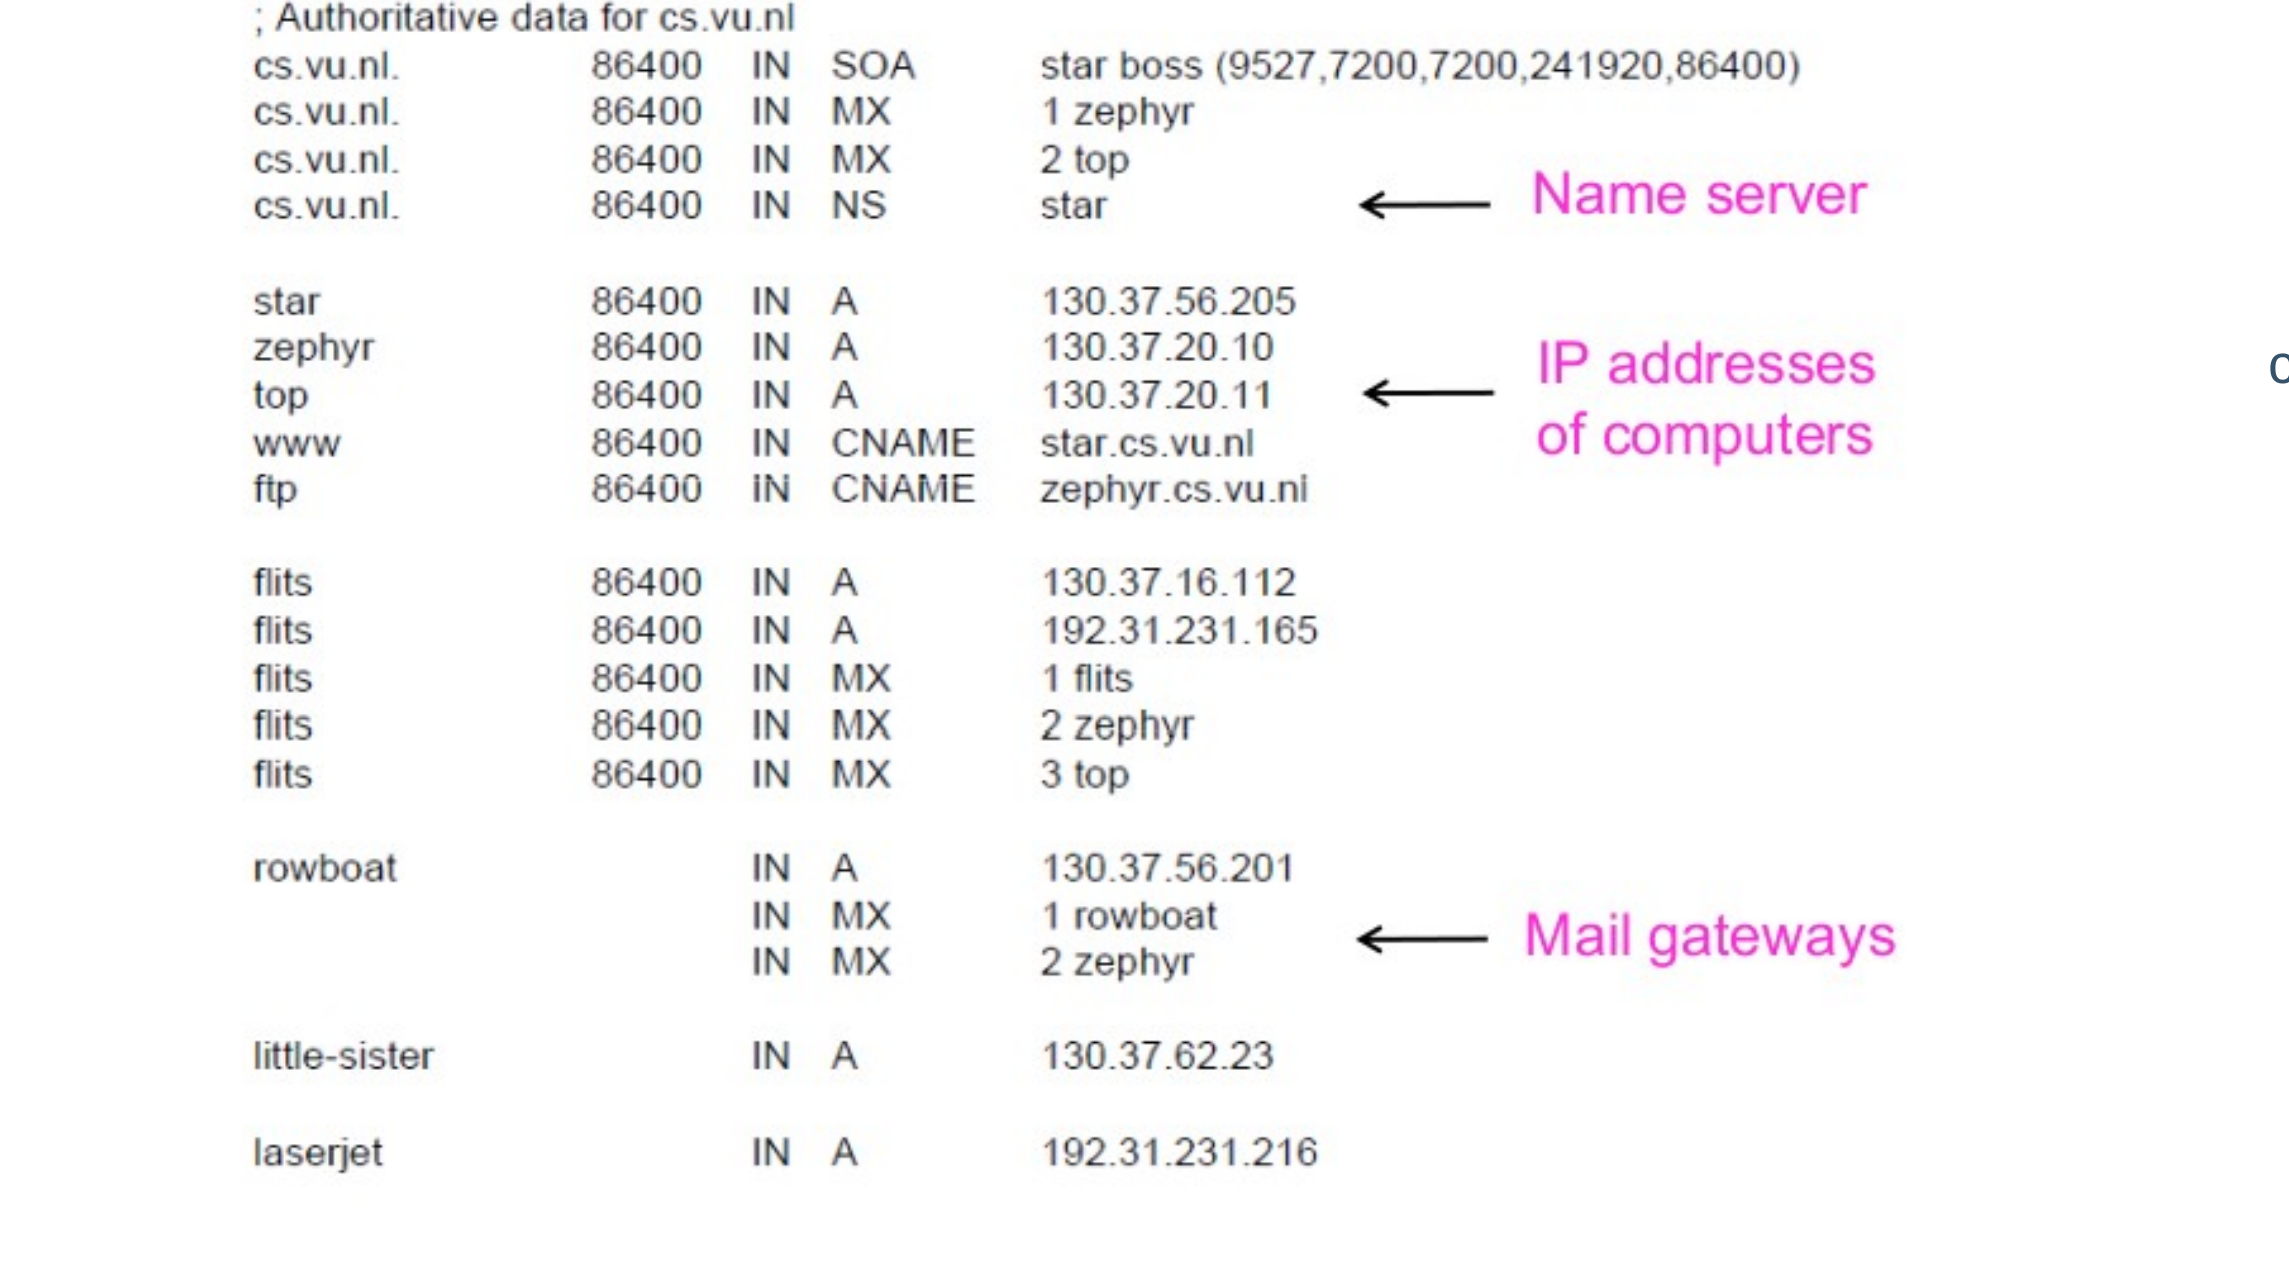
\includegraphics[width=0.62\linewidth]{cap07/rr_esempio.png}
\end{center}
Nel database autorevole per \texttt{cs.vu.nl} si trovano: il record \textbf{SOA} della zona, i record
\textbf{MX} (i server di posta, con la loro priorità: si prova prima quello con numero più basso), il record
\textbf{NS} (il name server \texttt{star}), i record \textbf{A} con gli indirizzi dei computer
(\texttt{star}, \texttt{zephyr}, \texttt{top}, \dots) e i \textbf{CNAME} che definiscono alias come
\texttt{www} e \texttt{ftp}.
\end{esempio}

% ══════════════════════════════════════════════════════════════
\section{I name server e le zone}
% ══════════════════════════════════════════════════════════════

Un unico server DNS centralizzato non avrebbe senso. Lo spazio dei nomi è quindi diviso in
\textbf{zone}.

\dfn{Zona}{
    Una \textbf{zona} è una porzione dello spazio dei nomi DNS, \textbf{senza sovrapposizioni} con le altre,
    i cui dati sono gestiti da uno o più \textbf{name server} (un \emph{primario} e uno o più
    \emph{secondari}). Come dividere il proprio dominio in zone lo decide l'amministratore.
}

\begin{figure}[H]
    \centering
    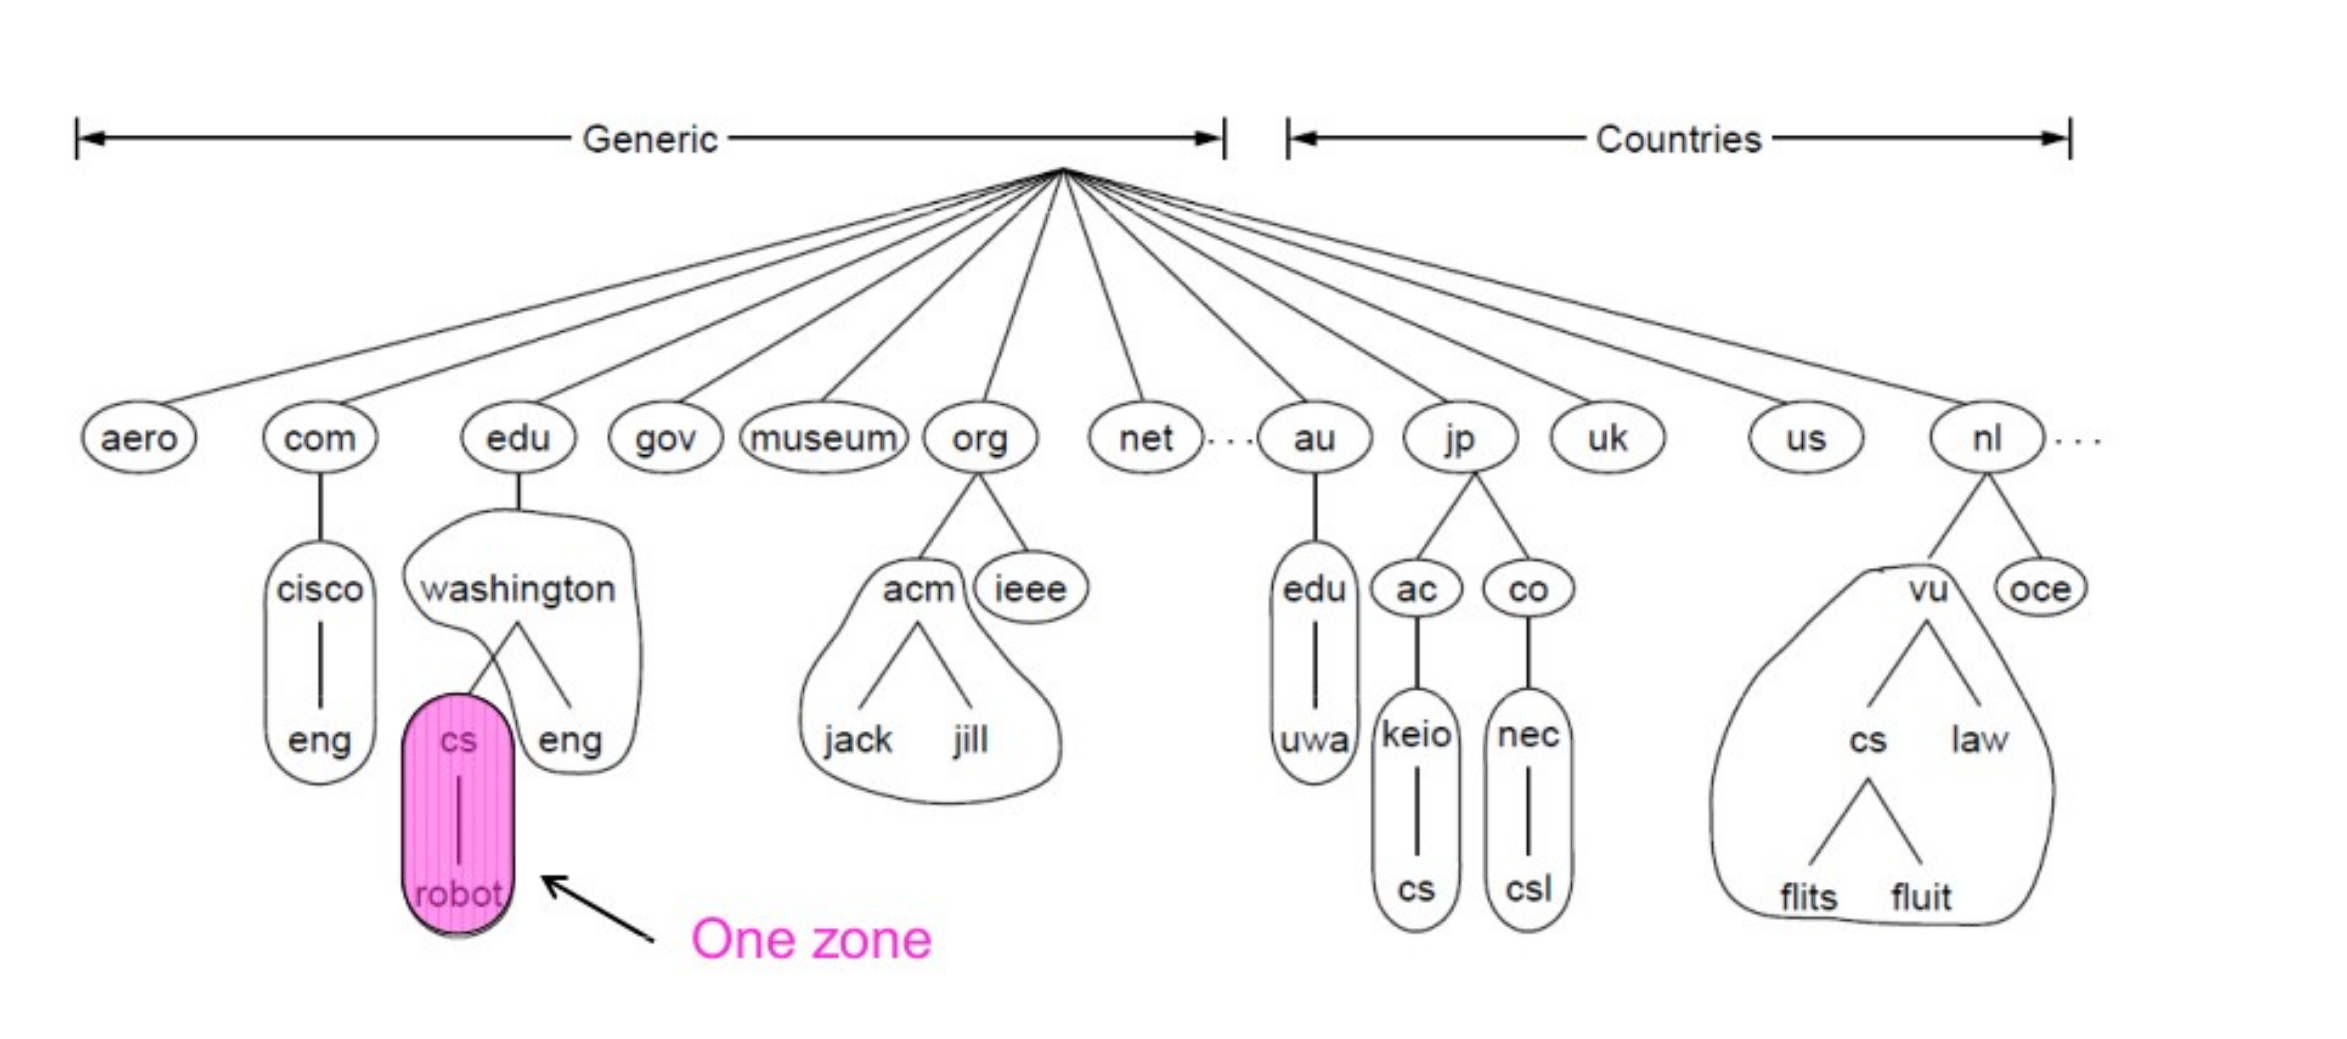
\includegraphics[width=0.72\linewidth]{cap07/zone_dns.png}
    \caption{Le zone (cerchiate) sono porzioni dello spazio dei nomi gestite da name server diversi.}
\end{figure}

\begin{figure}[H]
\centering
\begin{tikzpicture}[every node/.style={font=\footnotesize\sffamily}]
  \draw[thick, netblue, fill=cloudbg] (0,0) ellipse (4.2cm and 1.9cm);
  \node[text=netblue] at (3.6,1.6) {\texttt{jp}};
  \draw[thick, netgreen!70!black, fill=netgreen!10] (-0.4,-0.2) ellipse (3.2cm and 1.4cm);
  \node[text=netgreen!50!black] at (2.2,0.9) {\texttt{ac.jp}};
  \draw[thick, netorange, fill=netorange!15] (-0.9,-0.4) ellipse (2.2cm and 1cm);
  \node[text=netorange] at (0.6,0.35) {\texttt{kyushu-u.ac.jp}};
  \draw[thick, netorange, fill=netorange!45] (-1.6,-0.6) ellipse (1.1cm and 0.55cm);
  \node at (-1.6,-0.45) {\texttt{ofc}};
  \node at (-1.6,-0.8) {\scriptsize\texttt{hyoka}};
  \node[text width=6cm, align=left, anchor=west] at (4.6,0) {Può darsi che un server per \texttt{kyushu-u.ac.jp} abbia anche i record A, con autorità, per i nodi della sotto-zona (in arancione scuro), oppure che la sotto-zona \texttt{ofc} sia delegata a un altro server, come nell'esempio con \texttt{nslookup} alla fine del capitolo.};
\end{tikzpicture}
\caption{Domini annidati: ogni livello può gestire direttamente i nomi sottostanti o delegarli a una zona separata.}
\end{figure}

\dfn{Server autorevole}{
    Un name server è \textbf{autorevole} (\emph{authoritative}) per una zona se contiene i record originali di
    quella zona. Le risposte che fornisce su quella zona sono \textbf{risposte autorevoli}; quelle ottenute da
    una cache sono \textbf{non autorevoli}.
}

% ══════════════════════════════════════════════════════════════
\section{La risoluzione dei nomi}
% ══════════════════════════════════════════════════════════════

\subsection{La gerarchia dei server}

\begin{figure}[H]
\centering
\begin{tikzpicture}[every node/.style={font=\footnotesize\sffamily}, srv/.style={draw, rounded corners, minimum width=2.2cm, minimum height=0.75cm, align=center, fill=#1}]
  \node[srv=lphy] (root) at (0,0) {root server};
  \node[srv=lnet!60] (com) at (-4.5,-1.5) {server \texttt{.com}};
  \node[srv=lnet!60] (org) at (0,-1.5) {server \texttt{.org}};
  \node[srv=lnet!60] (edu) at (4.5,-1.5) {server \texttt{.edu}};
  \node[srv=ltra!60] (y) at (-6,-3) {yahoo.com}; \node[srv=ltra!60] (a) at (-3,-3) {amazon.com};
  \node[srv=ltra!60] (p) at (0,-3) {pbs.org};
  \node[srv=ltra!60] (n) at (3,-3) {nyu.edu}; \node[srv=ltra!60] (u) at (6,-3) {umass.edu};
  \foreach \x/\y in {root/com, root/org, root/edu, com/y, com/a, org/p, edu/n, edu/u} \draw[thick] (\x) -- (\y);
  \node[anchor=west] at (7.4,0) {1. radice};
  \node[anchor=west] at (7.4,-1.5) {2. top-level domain (TLD)};
  \node[anchor=west] at (7.4,-3) {3. server autorevoli};
\end{tikzpicture}
\caption{Una parte della gerarchia dei server DNS.}
\end{figure}

\begin{itemize}
    \item \textbf{Root server}: sono il punto di partenza quando non si ha nessuna informazione. Ci sono
          \textbf{13} ``root server'' logici, da \texttt{a.root-servers.net} a \texttt{m.root-servers.net},
          ciascuno \textbf{altamente replicato} in centinaia di copie nel mondo. Sono molto carichi, quindi di solito
          restituiscono informazioni sulle zone inferiori (i server dei TLD), non sui singoli record.
    \item \textbf{Server TLD}: responsabili dei domini di primo livello (\texttt{com}, \texttt{it}, \texttt{jp}, \dots).
    \item \textbf{Server autorevoli}: quelli delle organizzazioni, che contengono i record dei loro host.
\end{itemize}

\subsection{Il server DNS locale (resolver)}

\dfn{Server DNS locale}{
    Il \textbf{server DNS locale} (o \textbf{DNS resolver}) non appartiene strettamente alla gerarchia: è
    gestito tipicamente dall'ISP. Quando un host si collega a un ISP, riceve gli indirizzi di uno o più server
    DNS locali, di solito ``vicini''. Le interrogazioni dell'host vanno al server locale, che fa da
    \textbf{proxy} e le inoltra alla gerarchia.
}

Anche Google offre server di questo tipo in tutto il mondo (\emph{Google Public DNS}, agli indirizzi
\texttt{8.8.8.8} e \texttt{8.8.4.4}). Su molti sistemi Linux il resolver locale risponde all'indirizzo
\texttt{127.0.0.53}, porta 53: è un processo sulla macchina stessa che inoltra le richieste al server
indicato dal router.

\subsection{Query ricorsive e iterative}

La risoluzione procede così:

\begin{enumerate}
    \item l'host interroga il \textbf{server DNS locale};
    \item se il nome ricade nella zona di competenza del server locale, questo restituisce un record autorevole;
    \item altrimenti il server locale gestisce la richiesta ed effettua interrogazioni remote:
    \begin{itemize}
      \item se il server interrogato ha l'indirizzo, lo restituisce;
      \item altrimenti restituisce il \textbf{name server di una zona inferiore} a cui chiedere;
      \item il processo prosegue \textbf{iterativamente} finché l'indirizzo non viene trovato.
    \end{itemize}
\end{enumerate}

\dfn{Query ricorsiva e iterativa}{
    \begin{itemize}
      \item In una \textbf{query ricorsiva} chi riceve la domanda si fa carico di \textbf{tutta} la risoluzione e
            restituisce la risposta completa (o un errore).
      \item In una \textbf{query iterativa} chi riceve la domanda risponde con ciò che sa: la risposta, oppure
            \textbf{il nome del prossimo server} da interrogare.
    \end{itemize}
    Tipicamente l'host fa una query \textbf{ricorsiva} al server locale, e il server locale fa query
    \textbf{iterative} verso la gerarchia. I server più carichi, come quelli vicini alla radice, \textbf{non}
    accettano query ricorsive.
}

\begin{figure}[H]
\centering
\begin{tikzpicture}[every node/.style={font=\scriptsize\sffamily}]
  \begin{scope}
    \node[font=\footnotesize\bfseries\sffamily] at (2.3,3.6) {Iterativa (il server locale chiede a tutti)};
    \node (h) at (0,-1.6) {\icon[0.9cm]{pc}}; \node[below=-2pt of h] {host};
    \node (l) at (2.3,0) {\icon[0.6cm]{server}}; \node[below=-1pt of l] {server locale};
    \node (r) at (5,2.6) {\icon[0.5cm]{server}}; \node[right=0pt of r] {root};
    \node (t) at (5.6,0.6) {\icon[0.5cm]{server}}; \node[right=0pt of t] {TLD};
    \node (a) at (5,-1.6) {\icon[0.5cm]{server}}; \node[right=0pt of a] {autorevole};
    \draw[msg, netred] (h) -- node[left] {1} (l);
    \draw[msg, netblue] ([xshift=-2pt]l.north east) -- node[above left] {2} (r);
    \draw[msg, netgreen] (r) -- node[right] {3} ([xshift=6pt]l.north east);
    \draw[msg, netblue] (l) -- node[above] {4} (t);
    \draw[msg, netgreen] ([yshift=-6pt]t.west) -- node[below] {5} ([yshift=-6pt]l.east);
    \draw[msg, netblue] (l.south east) -- node[above right] {6} (a);
    \draw[msg, netgreen] ([xshift=-8pt]a.west) -- node[below] {7} ([xshift=4pt, yshift=-8pt]l.south east);
    \draw[msg, netred] ([xshift=-6pt]l.south) -- node[right] {8} ([xshift=8pt]h.north);
  \end{scope}
  \begin{scope}[xshift=8.6cm]
    \node[font=\footnotesize\bfseries\sffamily] at (2.3,3.6) {Ricorsiva (ognuno chiede al successivo)};
    \node (h) at (0,-1.6) {\icon[0.9cm]{pc}}; \node[below=-2pt of h] {host};
    \node (l) at (2.3,0) {\icon[0.6cm]{server}}; \node[below=-1pt of l] {server locale};
    \node (r) at (5,2.6) {\icon[0.5cm]{server}}; \node[right=0pt of r] {root};
    \node (t) at (5.6,0.6) {\icon[0.5cm]{server}}; \node[right=0pt of t] {TLD};
    \node (a) at (5,-1.6) {\icon[0.5cm]{server}}; \node[right=0pt of a] {autorevole};
    \draw[msg, netred] (h) -- node[left] {1} (l);
    \draw[msg, netblue] (l) -- node[above left] {2} (r);
    \draw[msg, netblue] ([xshift=-4pt]r.south) -- node[left] {3} ([xshift=-4pt]t.north);
    \draw[msg, netblue] ([xshift=-4pt]t.south) -- node[left] {4} ([xshift=-4pt]a.north);
    \draw[msg, netgreen] ([xshift=4pt]a.north) -- node[right] {5} ([xshift=4pt]t.south);
    \draw[msg, netgreen] ([xshift=4pt]t.north) -- node[right] {6} ([xshift=4pt]r.south);
    \draw[msg, netgreen] ([yshift=-5pt]r.west) -- node[below right] {7} ([xshift=8pt]l.north east);
    \draw[msg, netred] ([xshift=-6pt]l.south) -- node[right] {8} ([xshift=8pt]h.north);
  \end{scope}
\end{tikzpicture}
\caption{Query iterativa e ricorsiva a confronto: nel primo caso il server locale conduce la ricerca, nel secondo il carico ricade sui server della gerarchia.}
\end{figure}

\begin{figure}[H]
    \centering
    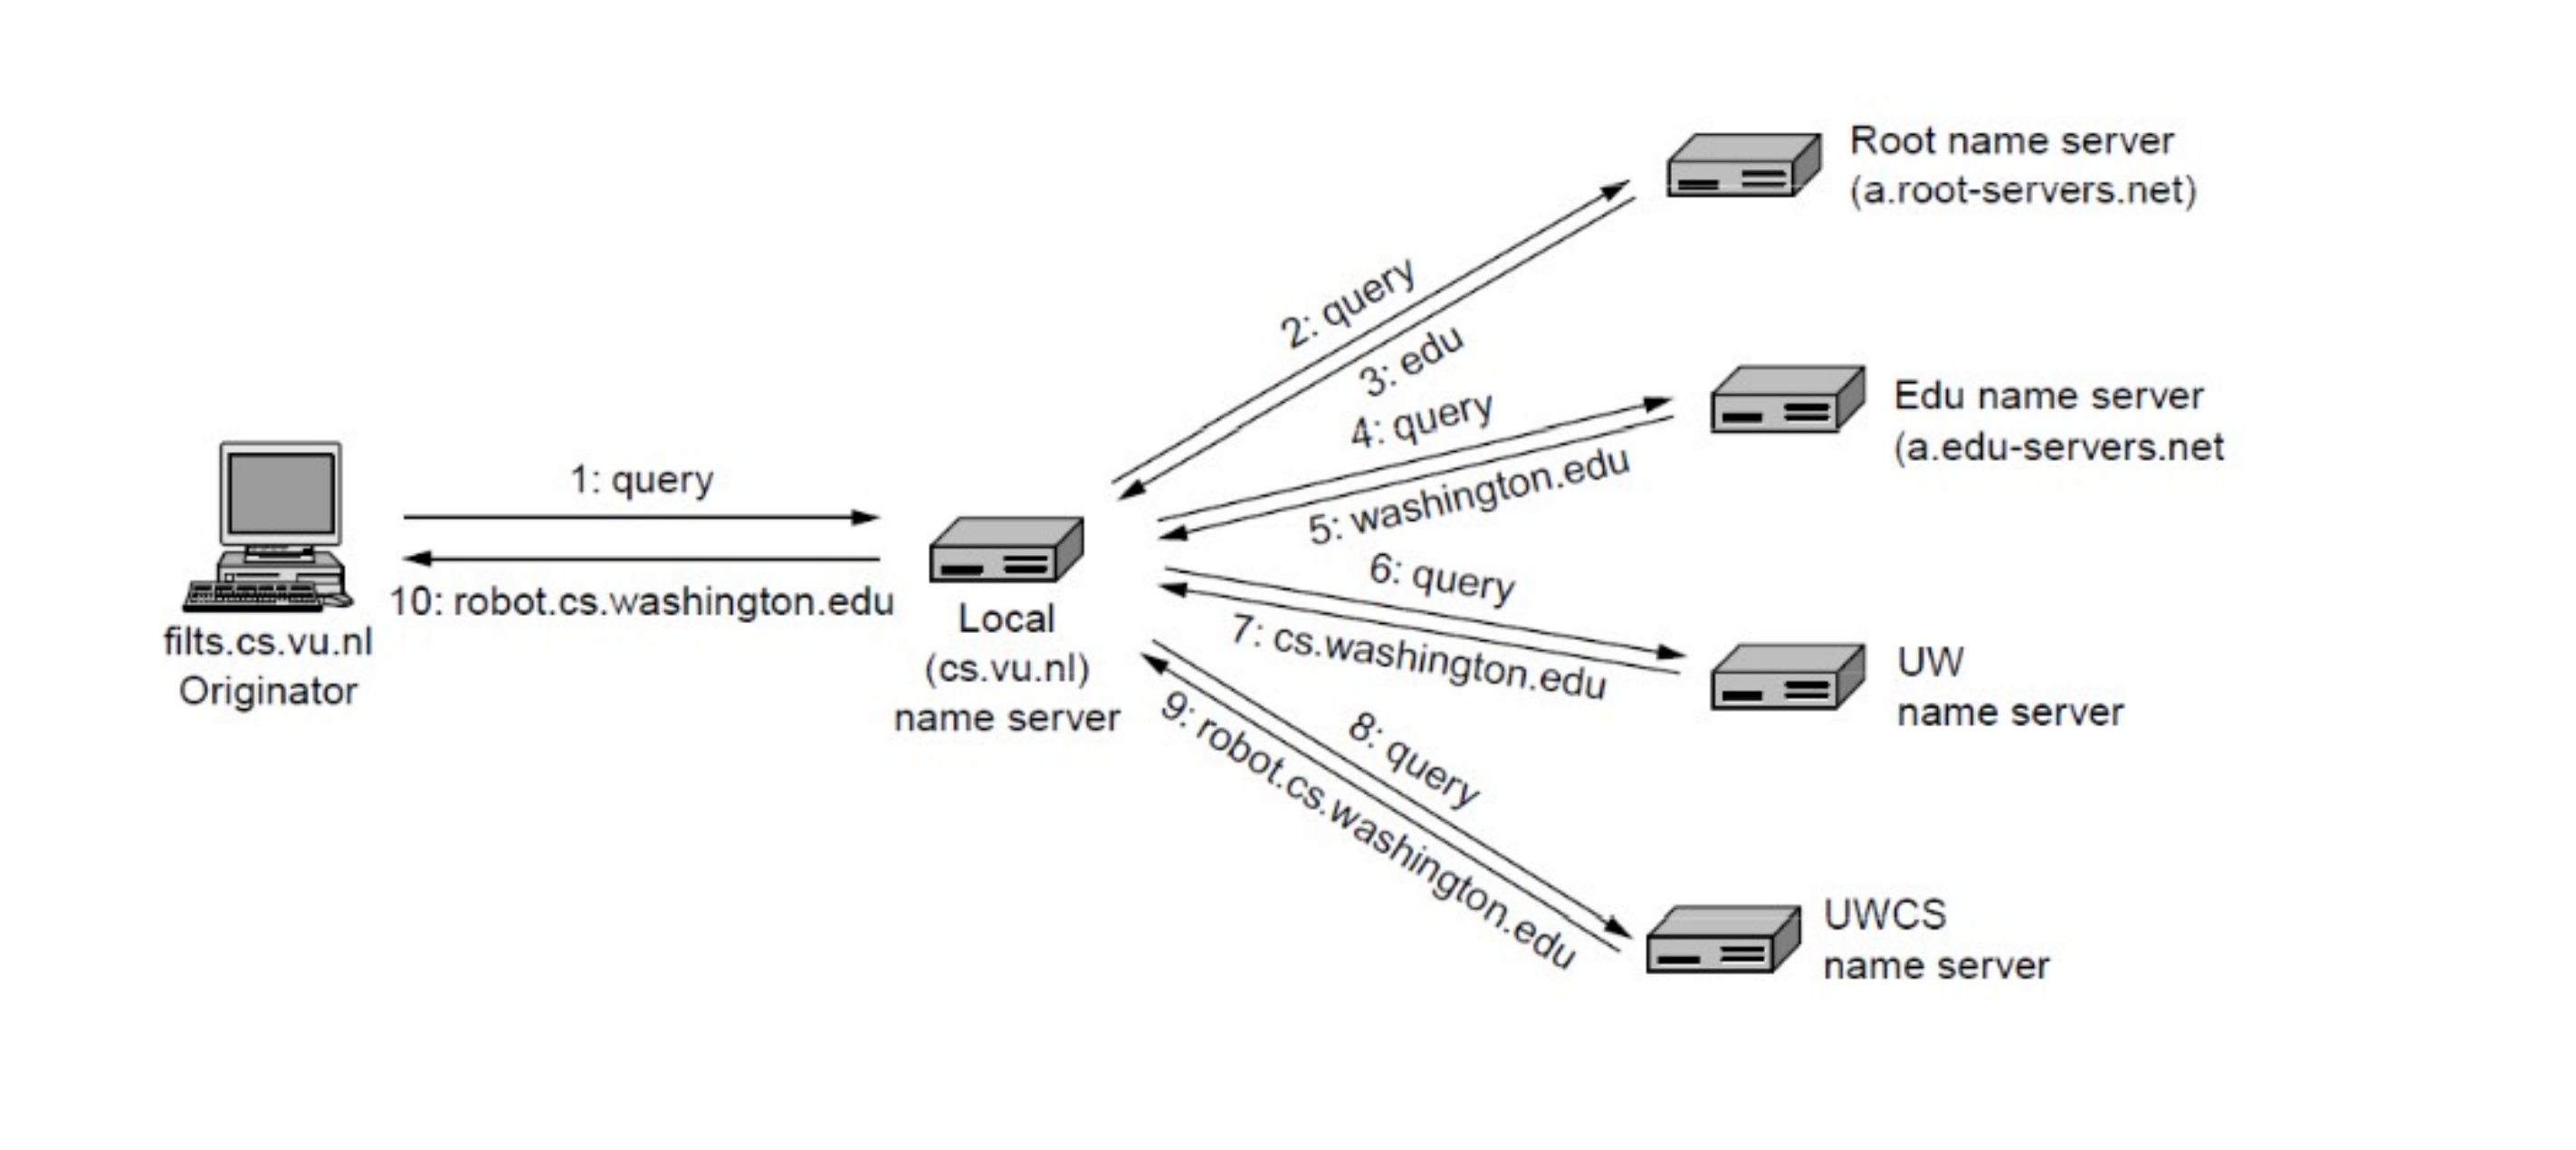
\includegraphics[width=0.72\linewidth]{cap07/risoluzione_esempio.png}
    \caption{L'host \texttt{flits.cs.vu.nl} risolve \texttt{robot.cs.washington.edu}: query ricorsiva (1, 10) verso il server locale, query iterative (2--9) verso root, \texttt{edu}, \texttt{washington.edu} e \texttt{cs.washington.edu}.}
\end{figure}

% ══════════════════════════════════════════════════════════════
\section{Il caching DNS}
% ══════════════════════════════════════════════════════════════

\begin{itemize}
    \item I record possono essere \textbf{autorevoli} o \textbf{in cache} (\emph{cached}).
    \item I record in cache \textbf{scadono}: è a questo che serve il TTL.
    \item Il caching migliora molto le prestazioni: \textbf{tutte le risposte} vengono memorizzate.
    \item Se il nome richiesto è in cache, il server locale risponde \textbf{subito}.
    \item Se arriva una richiesta per \texttt{cs.mit.edu} e il server conosce già l'indirizzo del server DNS di
          \texttt{mit.edu}, può interrogare direttamente quello, saltando root e TLD.
    \item I root server vengono interrogati solo quando non si ha \textbf{nessuna informazione} su un certo dominio.
\end{itemize}

\warning{Cache e TTL}{
    Se un sito cambia indirizzo IP, per un po' alcuni utenti continueranno a raggiungere quello vecchio: i
    resolver hanno ancora in cache il record, finché il suo TTL non scade. Per questo prima di un trasloco si
    abbassa il TTL dei record interessati.
}

% ══════════════════════════════════════════════════════════════
\section{I messaggi DNS}
% ══════════════════════════════════════════════════════════════

Richieste e risposte DNS hanno lo stesso formato (utile per leggere le catture con Wireshark):

\begin{figure}[H]
\centering
\begin{tikzpicture}[every node/.style={font=\scriptsize\sffamily}]
  \node[field, fill=lapp!60, minimum width=4.5cm] (id) at (0,0) {identificativo (16 bit)};
  \node[field, fill=lapp!60, minimum width=4.5cm, right=0pt of id] (fl) {flag (16 bit)};
  \node[field, fill=ltra!50, minimum width=4.5cm, below=0pt of id] (q) {n.\ domande};
  \node[field, fill=ltra!50, minimum width=4.5cm, right=0pt of q] (an) {n.\ RR risposta};
  \node[field, fill=ltra!50, minimum width=4.5cm, below=0pt of q] (au) {n.\ RR autorevoli};
  \node[field, fill=ltra!50, minimum width=4.5cm, right=0pt of au] (ad) {n.\ RR aggiuntivi};
  \node[field, fill=lnet!40, minimum width=9cm, anchor=north west] (s1) at (au.south west) {domande (nome e tipo richiesti)};
  \node[field, fill=lnet!40, minimum width=9cm, below=0pt of s1] (s2) {risposte (RR)};
  \node[field, fill=lnet!40, minimum width=9cm, below=0pt of s2] (s3) {autorità (RR dei server autorevoli)};
  \node[field, fill=lnet!40, minimum width=9cm, below=0pt of s3] (s4) {informazioni aggiuntive (per esempio i record A dei server)};
  \draw[decorate, decoration={brace, amplitude=5pt}] (6.9,0.3) -- (6.9,-1.6) node[midway, right=6pt] {header: 12 byte};
  \node[anchor=west, text width=5cm, align=left] at (9.4,-3.3) {flag: domanda o risposta, ricorsione desiderata, ricorsione disponibile, risposta autorevole};
\end{tikzpicture}
\caption{Formato dei messaggi DNS: l'identificativo permette di associare la risposta alla domanda.}
\end{figure}

% ══════════════════════════════════════════════════════════════
\section{Altri servizi del DNS}
% ══════════════════════════════════════════════════════════════

\subsection{Aliasing}

Il DNS offre un servizio di \textbf{alias}: a nomi complicati e lunghi (\textbf{canonici}) si associano nomi
più semplici (\textbf{alias}).

\begin{itemize}
    \item \textbf{Alias di host}: \texttt{relay1.west-coast.enterprise.com} può essere raggiunto come
          \texttt{www.enterprise.com} (record CNAME).
    \item \textbf{Alias di server di posta}: grazie ai record MX, l'indirizzo \texttt{bob@yahoo.com} funziona
          anche se il server di posta vero ha un nome complicato; e un'azienda può usare lo stesso nome per il
          sito Web e per la posta.
    \item Un'applicazione può comunque chiedere al DNS il \textbf{nome canonico} di un alias, oltre all'indirizzo IP.
\end{itemize}

\subsection{Distribuzione del carico}

\dfn{Round-robin DNS}{
    I siti molto frequentati (Google, Amazon, CNN, \dots) sono replicati su più server, ciascuno con un
    indirizzo IP diverso: al nome canonico è associato un \textbf{insieme di indirizzi}. Quando un client
    chiede quel nome, il server DNS restituisce tutti gli indirizzi ma \textbf{ne ruota l'ordine} a ogni
    risposta; poiché i client usano di solito il primo, il carico si distribuisce tra le repliche.
}

% ══════════════════════════════════════════════════════════════
\section{nslookup: interrogare il DNS a mano}
% ══════════════════════════════════════════════════════════════

Con \texttt{nslookup} si possono fare a mano le interrogazioni che fa un server DNS, e anche la
\textbf{ricerca inversa} (dal nome all'indirizzo). La sintassi è
\texttt{nslookup [-type=TIPO] nome [server]}.

\begin{esempio}{Record A: l'indirizzo di un nome}
\begin{lstlisting}
$ nslookup vatican.va
Server:    127.0.0.53
Address:   127.0.0.53#53

Non-authoritative answer:
Name:    vatican.va
Address: 185.152.70.106
\end{lstlisting}
Si recupera il record \textbf{A} di \texttt{vatican.va}. Il server interrogato è \texttt{127.0.0.53}, cioè il
resolver locale sulla porta 53. La risposta è \textbf{non autorevole}: viene da una cache, non dal server che
gestisce la zona. Il resolver locale ha condotto l'intera risoluzione con query iterative, mentre l'host gli ha
fatto una query ricorsiva.
\end{esempio}

\begin{esempio}{Record NS e SOA}
\begin{lstlisting}
$ nslookup -type=NS vatican.va
Non-authoritative answer:
vatican.va  nameserver = a.nic.va.
vatican.va  nameserver = b.nic.va.
vatican.va  nameserver = c.nic.va.
vatican.va  nameserver = osiris.namex.it.
vatican.va  nameserver = seth.namex.it.

$ nslookup -type=SOA vatican.va
Non-authoritative answer:
vatican.va
    origin = a.nic.va
    mail addr = dnsop.net.va
    serial = 2025062401
    refresh = 14400
    retry = 3600
    expire = 1209600
    minimum = 3600
\end{lstlisting}
La prima query elenca i \textbf{name server} del dominio. La seconda chiede il record \textbf{SOA}, che indica il
server principale autorevole (\texttt{origin = a.nic.va}) e i parametri della zona. La riga
``\emph{Authoritative answers can be found from:}'' senza elenco è normale con i resolver intermedi, che
spesso non includono i record dei server autorevoli.
\end{esempio}

\begin{esempio}{Interrogare direttamente il server autorevole}
\begin{lstlisting}
$ nslookup -type=A a.nic.va
Name:    a.nic.va
Address: 212.77.0.110

$ nslookup -type=A vatican.va 212.77.0.110
Server:  212.77.0.110
Address: 212.77.0.110#53
Non-authoritative answer:
Name:    vatican.va
Address: 185.152.70.106
\end{lstlisting}
Prima si trova l'indirizzo del server principale, poi lo si interroga direttamente (secondo argomento). In
teoria la risposta dovrebbe essere autorevole, ma alcuni server non impostano il flag \emph{Authoritative
Answer} (per configurazione, inoltro o motivi di sicurezza).
\end{esempio}

\subsection{La risoluzione iterativa fatta a mano}

Proviamo a risolvere \texttt{hyoka.ofc.kyushu-u.ac.jp} \textbf{ignorando il server locale}, come farebbe un
server DNS senza nulla in cache: si parte da un root server e si scende.

\begin{figure}[H]
\centering
\begin{tikzpicture}[every node/.style={font=\scriptsize\sffamily}, st/.style={draw, rounded corners, fill=#1, minimum width=3.1cm, minimum height=0.8cm, align=center}]
  \node[st=lphy] (s1) at (0,0) {\texttt{c.root-servers.net}};
  \node[st=lnet!50] (s2) at (5.2,0) {\texttt{b.dns.jp}};
  \node[st=ltra!50] (s3) at (10.4,0) {\texttt{ns2.kyushu-u.ac.jp}};
  \node[st=lapp!50] (s4) at (15.6,0) {\texttt{ns.jimu.kyushu-u.ac.jp}};
  \draw[msg, very thick] (s1) -- node[above, text width=2.6cm, align=center] {``chiedi ai server di \texttt{jp}''} (s2);
  \draw[msg, very thick] (s2) -- node[above, text width=2.6cm, align=center] {``chiedi ai server di \texttt{kyushu-u.ac.jp}''} (s3);
  \draw[msg, very thick] (s3) -- node[above, text width=2.6cm, align=center] {``chiedi a quelli di \texttt{ofc.kyushu-u.ac.jp}''} (s4);
  \node[below=4pt of s4, text=netgreen!60!black, font=\scriptsize\bfseries\sffamily] {133.5.40.197};
\end{tikzpicture}
\caption{Ogni server non conosce la risposta, ma sa a chi chiedere un livello più in basso.}
\end{figure}

\begin{lstlisting}
$ nslookup -type=A hyoka.ofc.kyushu-u.ac.jp c.root-servers.net
*** Can't find hyoka.ofc.kyushu-u.ac.jp: No answer        # il root non sa nulla

$ nslookup -type=NS hyoka.ofc.kyushu-u.ac.jp c.root-servers.net
Authoritative answers can be found from:
jp  nameserver = a.dns.jp.   (... b.dns.jp ... h.dns.jp)  # ma conosce i server di jp
b.dns.jp  internet address = 202.12.30.131

$ nslookup -type=NS hyoka.ofc.kyushu-u.ac.jp b.dns.jp
Authoritative answers can be found from:
kyushu-u.ac.jp  nameserver = ns1.kyushu-u.ac.jp.          # jp conosce i server di kyushu-u
kyushu-u.ac.jp  nameserver = ns2.kyushu-u.ac.jp.
ns2.kyushu-u.ac.jp  internet address = 133.5.1.9

$ nslookup -type=NS hyoka.ofc.kyushu-u.ac.jp ns2.kyushu-u.ac.jp
Authoritative answers can be found from:
ofc.kyushu-u.ac.jp  nameserver = ns.jimu.kyushu-u.ac.jp.  # sotto-zona ofc
ns.jimu.kyushu-u.ac.jp  internet address = 133.5.40.1

$ nslookup -type=A hyoka.ofc.kyushu-u.ac.jp ns.jimu.kyushu-u.ac.jp
Name:    hyoka.ofc.kyushu-u.ac.jp
Address: 133.5.40.197                                     # finalmente il server autorevole
\end{lstlisting}

\info{Da provare}{
    Si possono interrogare i server in alto nella gerarchia (compresi i root server) con l'opzione
    \texttt{-norecurse}, e poi senza, confrontando i risultati. Altri esempi utili: \texttt{nslookup -type=MX
    mit.edu} (i server di posta) e \texttt{nslookup -type=NS mit.edu} (i server DNS con autorità).
}

% ══════════════════════════════════════════════════════════════
\section{Riepilogo}
% ══════════════════════════════════════════════════════════════

\riepilogo{
\begin{itemize}
    \item Il \textbf{DNS} traduce nomi in indirizzi IP: è un protocollo applicativo client-server su \textbf{UDP,
          porta 53}, realizzato come database \textbf{distribuito} e \textbf{gerarchico}.
    \item Lo spazio dei nomi è un albero (radice, TLD, sottodomini) diviso in \textbf{zone}, ciascuna con i propri
          name server \textbf{autorevoli}.
    \item I dati sono \textbf{resource record} (NAME, TTL, CLASS, TYPE, VALUE): A, AAAA, NS, CNAME, MX, SOA, PTR, \dots
    \item L'host fa una query \textbf{ricorsiva} al server locale; il server locale fa query \textbf{iterative} a
          root, TLD e server autorevoli.
    \item Il \textbf{caching} (con scadenza data dal TTL) rende il DNS veloce; il DNS offre anche \textbf{alias} e
          \textbf{distribuzione del carico}.
\end{itemize}
}
  % DNS
  \chapter{Programmazione di rete: i socket in C}

Finora abbiamo visto applicazioni e protocolli esistenti. Ora vediamo come \textbf{creare} un'applicazione
di rete. Quasi tutte sono fatte di un programma lato client e di un programma lato server: quando li
eseguiamo nascono un processo client e un processo server, che comunicano \textbf{leggendo e scrivendo sui
socket}.

% ══════════════════════════════════════════════════════════════
\section{Le scelte di progetto}
% ══════════════════════════════════════════════════════════════

\subsection{Protocolli aperti e proprietari}

\begin{itemize}
    \item \textbf{Protocolli aperti}: le regole sono pubbliche (per esempio in un RFC). Un client scritto da noi
          può parlare con un server scritto da altri, purché entrambi rispettino lo standard (un nostro client HTTP
          parla con Apache).
    \item \textbf{Protocolli proprietari}: regole ``fatte in casa'', non pubblicate. Client e server li scrive lo
          stesso sviluppatore, che ha pieno controllo ma deve fare tutto da sé.
\end{itemize}

\subsection{La scelta del protocollo di trasporto}

\begin{itemize}
    \item \textbf{TCP}: orientato alla connessione, offre un \textbf{canale affidabile a flusso di byte} tra i due end system.
    \item \textbf{UDP}: senza connessione, invia \textbf{pacchetti indipendenti} da un end system all'altro, senza
          alcuna garanzia di consegna.
\end{itemize}

% ══════════════════════════════════════════════════════════════
\section{Dove stanno i socket nella pila}
% ══════════════════════════════════════════════════════════════

\begin{figure}[H]
\centering
\begin{tikzpicture}[every node/.style={font=\small\sffamily}]
  \node[lay app, minimum width=3.6cm, minimum height=0.9cm] (a) at (0,1.8) {Applicazione};
  \node[lay tra, minimum width=3.6cm, minimum height=0.9cm] (t) at (0,0.9) {Trasporto (TCP/UDP)};
  \node[lay net, minimum width=3.6cm, minimum height=0.9cm] (n) at (0,0) {Rete (IP)};
  \node[lay link, minimum width=3.6cm, minimum height=0.9cm] (l) at (0,-0.9) {Accesso (link + fisico)};
  \node[draw, fill=lapp!40, rounded corners, minimum width=3.4cm, minimum height=0.9cm] (my) at (6,1.8) {la vostra applicazione};
  \node[draw, fill=white, very thick, draw=netred, rounded corners, minimum width=3.4cm, minimum height=0.5cm] (api) at (6,1.1) {\textbf{API dei socket}};
  \node[draw, fill=lphy!50, rounded corners, minimum width=3.4cm, minimum height=1.8cm, align=center] (os) at (6,-0.2) {sistema operativo\\+ hardware};
  \draw[dashed, netred, thick] (-2.4,1.35) -- (8.2,1.35);
  \node[text=netred, anchor=west, font=\scriptsize\sffamily] at (8.3,1.35) {socket};
  \draw[decorate, decoration={brace, amplitude=5pt, mirror}] (-2.1,1.3) -- (-2.1,-1.35) node[midway, left=6pt, align=center, font=\scriptsize\sffamily] {implementati\\dal sistema\\operativo};
\end{tikzpicture}
\caption{Dove sono implementati gli strati: l'applicazione è nostra, trasporto e rete stanno nel sistema operativo e si usano attraverso l'API dei socket.}
\end{figure}

I socket sono l'elemento centrale per creare applicazioni di rete: realizzano, come una scatola nera,
le funzionalità di \textbf{trasporto} (TCP/UDP) e di \textbf{rete} (IP). Esistono librerie e
\emph{middleware} che ``avvolgono'' i socket semplificandone l'uso e offrendo funzioni più complesse, ma le
API di base sono ancora molto usate.

Le API per socket TCP e UDP esistono in quasi tutti i linguaggi e sistemi operativi (C, C++, C\#, Java,
Python, \dots). Nel mondo Unix si usano i \textbf{socket di Berkeley} (detti anche socket BSD o POSIX): API
native in C, le stesse che useremo noi.

\info{Tutto è un file}{
    I socket seguono la filosofia Unix per cui ``\emph{tutto è un file}'': un socket è identificato da un
    \textbf{file descriptor}, come un file aperto, e si può chiudere con \texttt{close()} o leggere con
    \texttt{read()}.
}

% ══════════════════════════════════════════════════════════════
\section{UDP e TCP: le due sequenze}
% ══════════════════════════════════════════════════════════════

\begin{figure}[H]
\centering
\begin{tikzpicture}[every node/.style={font=\scriptsize\sffamily}, st/.style={draw, rounded corners, fill=#1, minimum width=2.2cm, minimum height=0.6cm, align=center}]
  \begin{scope}
    \node[font=\small\bfseries\sffamily] at (1.4,1) {Senza connessione (UDP)};
    \node[font=\bfseries\sffamily] at (0,0.4) {Client}; \node[font=\bfseries\sffamily] at (2.8,0.4) {Server};
    \node[st=lapp!40] (c1) at (0,-0.2) {crea socket}; \node[st=lapp!40] (s1) at (2.8,-0.2) {crea socket};
    \node[st=ltra!40] (c3) at (0,-1.8) {invia messaggio}; \node[st=ltra!40] (s3) at (2.8,-1.8) {legge messaggio};
    \node[st=ltra!40] (c4) at (0,-2.6) {legge risposta}; \node[st=ltra!40] (s4) at (2.8,-2.6) {invia risposta};
    \node[st=lnet!40] (c5) at (0,-3.4) {chiude socket};
    \foreach \a/\b in {c1/c3, c3/c4, c4/c5, s1/s3, s3/s4} \draw[-{Stealth}] (\a) -- (\b);
    \draw[msg, netblue] (c3) -- (s3); \draw[msg, netgreen] (s4) -- (c4);
  \end{scope}
  \begin{scope}[xshift=9cm]
    \node[font=\small\bfseries\sffamily] at (1.4,1) {Orientata alla connessione (TCP)};
    \node[font=\bfseries\sffamily] at (0,0.4) {Client}; \node[font=\bfseries\sffamily] at (2.8,0.4) {Server};
    \node[st=lapp!40] (c1) at (0,-0.2) {crea socket}; \node[st=lapp!40] (s1) at (2.8,-0.2) {crea socket};
    \node[st=netred!15] (c2) at (0,-1.0) {connetti}; \node[st=netred!15] (s2) at (2.8,-1.0) {attende\\connessioni};
    \node[st=ltra!40] (c3) at (0,-1.8) {invia messaggio}; \node[st=ltra!40] (s3) at (2.8,-1.8) {legge messaggio};
    \node[st=ltra!40] (c4) at (0,-2.6) {legge risposta}; \node[st=ltra!40] (s4) at (2.8,-2.6) {invia risposta};
    \node[st=lnet!40] (c5) at (0,-3.4) {chiude socket}; \node[st=lnet!40] (s5) at (2.8,-3.4) {chiude socket\\del client};
    \foreach \a/\b in {c1/c2, c2/c3, c3/c4, c4/c5, s1/s2, s2/s3, s3/s4, s4/s5} \draw[-{Stealth}] (\a) -- (\b);
    \draw[msg, netred, {Stealth}-{Stealth}] (c2) -- (s2);
    \draw[msg, netblue] (c3) -- (s3); \draw[msg, netgreen] (s4) -- (c4);
  \end{scope}
  \foreach \y/\t in {-0.2/creazione, -1.0/connessione, -2.2/messaggi, -3.4/distruzione} \node[font=\scriptsize\itshape\sffamily, text=black!60] at (6.2,\y) {\t};
\end{tikzpicture}
\caption{Le fasi di una comunicazione senza connessione e con connessione.}
\end{figure}

% ══════════════════════════════════════════════════════════════
\section{Le strutture dati}
% ══════════════════════════════════════════════════════════════

I socket del dominio Internet in C usano alcune strutture per descrivere indirizzi e porte degli host:

\begin{lstlisting}[language={[POSIX]C}]
#include <netinet/in.h>
#include <arpa/inet.h>     // per inet_addr()
#include <sys/types.h>     // alcuni tipi personalizzati

struct sockaddr_in {
    short          sin_family;  // famiglia dell'indirizzo, di solito AF_INET (IPv4)
    unsigned short sin_port;    // numero di porta, per esempio htons(3490)
    struct in_addr sin_addr;    // indirizzo IP (vedi sotto)
    char           sin_zero[8]; // zeri: la struttura ha la stessa dimensione di sockaddr
};

struct in_addr {
    unsigned long s_addr;       // indirizzo IP: inet_addr("...") oppure INADDR_ANY
};
\end{lstlisting}

\begin{itemize}
    \item \texttt{sin\_zero} serve solo a rendere la struttura grande quanto la generica \texttt{struct sockaddr}:
          per questo alle funzioni si passa \texttt{(struct sockaddr *)\&indirizzo}.
    \item \texttt{inet\_addr("192.168.1.10")} converte un indirizzo in notazione puntata nel formato binario;
          \texttt{INADDR\_ANY} significa ``qualsiasi indirizzo di questa macchina''.
\end{itemize}

\warning{L'ordine dei byte: htons()}{
    Macchine diverse memorizzano i numeri su più byte in ordine diverso (\emph{little endian} o \emph{big endian}).
    In rete si usa per convenzione il \textbf{network byte order} (big endian). Per questo porte e indirizzi vanno
    convertiti: \texttt{htons()} (\emph{host to network short}) per le porte a 16 bit, \texttt{htonl()} per i
    valori a 32 bit, e \texttt{ntohs()}/\texttt{ntohl()} per il percorso inverso.
    \begin{center}
    \begin{tikzpicture}[every node/.style={font=\scriptsize\ttfamily}]
      \node[anchor=east, font=\scriptsize\sffamily] at (-0.2,0) {porta 8080 = 0x1F90, su x86:};
      \node[field, fill=lapp!50, minimum width=1cm] at (0.5,0) {90}; \node[field, fill=lnet!50, minimum width=1cm] at (1.5,0) {1F};
      \node[anchor=east, font=\scriptsize\sffamily] at (-0.2,-0.8) {dopo htons(8080), in rete:};
      \node[field, fill=lnet!50, minimum width=1cm] at (0.5,-0.8) {1F}; \node[field, fill=lapp!50, minimum width=1cm] at (1.5,-0.8) {90};
    \end{tikzpicture}
    \end{center}
}

% ══════════════════════════════════════════════════════════════
\section{Le funzioni di base}
% ══════════════════════════════════════════════════════════════

\subsection{Creazione del socket: socket()}

\begin{lstlisting}[language={[POSIX]C}]
#include <sys/socket.h>
int sockfd = socket(int domain, int type, int protocol);
\end{lstlisting}

\begin{itemize}
    \item \texttt{domain}: la famiglia di indirizzi, come nella struttura (\texttt{AF\_INET});
    \item \texttt{type}: il tipo di socket: \texttt{SOCK\_STREAM} $\rightarrow$ \textbf{TCP}, \texttt{SOCK\_DGRAM}
          $\rightarrow$ \textbf{UDP};
    \item \texttt{protocol}: un protocollo specifico da usare nel socket; di solito \texttt{0} (quello di default);
    \item \texttt{sockfd}: il \textbf{file descriptor} del nuovo socket (negativo in caso di errore).
\end{itemize}

\subsection{Associazione a indirizzo e porta: bind()}

\begin{lstlisting}[language={[POSIX]C}]
#include <sys/socket.h>
int val = bind(int socket, const struct sockaddr *address, socklen_t address_len);
\end{lstlisting}

\begin{itemize}
    \item \texttt{socket}: il file descriptor del socket da associare;
    \item \texttt{address}: puntatore a una \texttt{sockaddr} con porta e indirizzo su cui mettersi in ascolto;
          spesso \texttt{sin\_addr} è \texttt{INADDR\_ANY}, così si ascolta su tutti gli indirizzi della macchina;
    \item \texttt{address\_len}: la dimensione della struttura (con \texttt{sizeof()});
    \item \texttt{val}: 0 in caso di successo, $-1$ altrimenti.
\end{itemize}

\warning{bind() serve al server}{
    Il server \textbf{deve} associare il socket a una porta precisa (i client devono sapere dove trovarlo).
    Sul client \texttt{bind()} è \textbf{facoltativa}: se non la si chiama, il sistema operativo sceglie
    automaticamente una porta libera.
}

\subsection{Invio e ricezione in UDP: sendto() e recvfrom()}

\begin{lstlisting}[language={[POSIX]C}]
#include <sys/socket.h>
int ob = sendto(int osock, const void *obuf, size_t olen, int oflags,
                const struct sockaddr *oaddr, socklen_t oaddr_len);
int ib = recvfrom(int isock, void *ibuf, size_t ilen, int iflags,
                  struct sockaddr *iaddr, socklen_t *iaddr_len);
\end{lstlisting}

\begin{itemize}
    \item \texttt{osock}/\texttt{isock}: il socket su cui inviare/ricevere;
    \item \texttt{obuf}/\texttt{ibuf}: il buffer con il messaggio da inviare / dove mettere quello ricevuto;
    \item \texttt{olen}/\texttt{ilen}: la lunghezza in byte;
    \item \texttt{oflags}/\texttt{iflags}: opzioni, di solito \texttt{0} (oppure \texttt{MSG\_WAITALL} per aspettare
          tutti i byte richiesti);
    \item \texttt{oaddr}: l'indirizzo del \textbf{destinatario}; \texttt{iaddr}: dove la funzione \textbf{scrive}
          l'indirizzo del mittente;
    \item \texttt{ob}/\texttt{ib}: il numero di byte effettivamente inviati/ricevuti.
\end{itemize}

\info{Perché in UDP serve l'indirizzo ogni volta}{
    In UDP non c'è connessione: il socket non ``sa'' con chi sta parlando. Per questo \texttt{sendto()} vuole
    l'indirizzo del destinatario a ogni invio, e \texttt{recvfrom()} restituisce l'indirizzo di chi ha mandato il
    messaggio, così che il server possa rispondergli.
}

\subsection{Chiusura: close()}

\begin{lstlisting}[language={[POSIX]C}]
#include <unistd.h>
int val = close(int socket);   // 0 in caso di successo, -1 altrimenti
\end{lstlisting}

% ══════════════════════════════════════════════════════════════
\section{Esempio completo: client e server UDP}
% ══════════════════════════════════════════════════════════════

\begin{figure}[H]
\centering
\begin{tikzpicture}[yscale=0.7, every node/.style={font=\scriptsize\ttfamily}]
  \node[font=\footnotesize\bfseries\sffamily] at (0,0.6) {Client}; \node[font=\footnotesize\bfseries\sffamily] at (6,0.6) {Server};
  \draw[thick, black!50] (0,0) -- (0,-7.3); \draw[thick, black!50] (6,0) -- (6,-7.3);
  \node[fill=white, draw, rounded corners] at (0,-0.4) {socket()}; \node[fill=white, draw, rounded corners] at (6,-0.4) {socket()};
  \node[fill=white, draw, rounded corners] at (6,-1.4) {bind()};
  \node[fill=white, draw, rounded corners] (rf) at (6,-2.8) {recvfrom()};
  \node[fill=white, draw, rounded corners] (st) at (0,-2.4) {sendto()};
  \draw[msg, netblue] (st) -- node[above, sloped, font=\scriptsize\sffamily] {``Hello from client''} (rf);
  \node[fill=white, draw, rounded corners] (st2) at (6,-4.2) {sendto()};
  \node[fill=white, draw, rounded corners] (rf2) at (0,-4.8) {recvfrom()};
  \draw[msg, netgreen] (st2) -- node[above, sloped, font=\scriptsize\sffamily] {``Hello from server''} (rf2);
  \node[fill=white, draw, rounded corners] at (0,-6.5) {close()}; \node[fill=white, draw, rounded corners] at (6,-6.5) {close()};
  \node[anchor=west, font=\scriptsize\sffamily, text width=6cm, align=left] at (7,-2.8) {\textbf{recvfrom} si blocca finché non arriva un messaggio e restituisce IP e porta del client};
  \draw[{Stealth}-{Stealth}, dashed, black!50] (-0.8,-2.2) -- node[left, font=\scriptsize\sffamily, align=center] {si può\\ripetere} (-0.8,-5.0);
\end{tikzpicture}
\caption{La sequenza di chiamate per un semplice scambio UDP.}
\end{figure}

\begin{lstlisting}[language={[POSIX]C}, style=wnumbers, title={udp\_server.c}]
#include <stdio.h>
#include <stdlib.h>
#include <string.h>
#include <unistd.h>
#include <arpa/inet.h>
#include <sys/socket.h>

#define PORT    8080
#define MAXLINE 1024

int main(void) {
    int sockfd;
    char buffer[MAXLINE];
    const char *hello = "Hello from server";
    struct sockaddr_in servaddr, cliaddr;

    // 1. Creazione del socket UDP
    if ((sockfd = socket(AF_INET, SOCK_DGRAM, 0)) < 0) {
        perror("socket creation failed");
        exit(EXIT_FAILURE);
    }

    memset(&servaddr, 0, sizeof(servaddr));
    memset(&cliaddr, 0, sizeof(cliaddr));
    servaddr.sin_family      = AF_INET;
    servaddr.sin_addr.s_addr = INADDR_ANY;     // tutte le interfacce
    servaddr.sin_port        = htons(PORT);

    // 2. Associazione alla porta 8080
    if (bind(sockfd, (const struct sockaddr *)&servaddr, sizeof(servaddr)) < 0) {
        perror("bind failed");
        exit(EXIT_FAILURE);
    }

    // 3. Ricezione: cliaddr viene riempita con indirizzo e porta del client
    socklen_t len = sizeof(cliaddr);
    int n = recvfrom(sockfd, buffer, MAXLINE - 1, 0,
                     (struct sockaddr *)&cliaddr, &len);
    buffer[n] = '\0';
    printf("Ricevuto \"%s\"\n", buffer);

    // 4. Risposta proprio a chi ci ha scritto
    sendto(sockfd, hello, strlen(hello), 0, (const struct sockaddr *)&cliaddr, len);
    printf("Hello message sent.\n");

    close(sockfd);
    return 0;
}
\end{lstlisting}

\begin{lstlisting}[language={[POSIX]C}, style=wnumbers, title={udp\_client.c}]
#include <stdio.h>
#include <stdlib.h>
#include <string.h>
#include <unistd.h>
#include <arpa/inet.h>
#include <sys/socket.h>

#define PORT    8080
#define MAXLINE 1024

int main(void) {
    int sockfd;
    char buffer[MAXLINE];
    const char *hello = "Hello from client";
    struct sockaddr_in servaddr;

    if ((sockfd = socket(AF_INET, SOCK_DGRAM, 0)) < 0) {
        perror("socket creation failed");
        exit(EXIT_FAILURE);
    }

    memset(&servaddr, 0, sizeof(servaddr));
    servaddr.sin_family      = AF_INET;
    servaddr.sin_port        = htons(PORT);
    servaddr.sin_addr.s_addr = inet_addr("127.0.0.1");  // server sulla stessa macchina

    // Nessuna bind(): la porta del client la sceglie il sistema operativo
    sendto(sockfd, hello, strlen(hello), 0, (const struct sockaddr *)&servaddr, sizeof(servaddr));
    printf("Hello message sent.\n");

    socklen_t len = sizeof(servaddr);
    int n = recvfrom(sockfd, buffer, MAXLINE - 1, 0, (struct sockaddr *)&servaddr, &len);
    buffer[n] = '\0';
    printf("Ricevuto \"%s\"\n", buffer);

    close(sockfd);
    return 0;
}
\end{lstlisting}

\begin{lstlisting}[language=bash, title={Compilazione ed esecuzione, in due terminali}]
$ gcc -o udp_server udp_server.c
$ gcc -o udp_client udp_client.c
$ ./udp_server        # terminale 1: resta in attesa
$ ./udp_client        # terminale 2
\end{lstlisting}

\warning{Parlare con un altro computer}{
    Nelle trasparenze il client usa \texttt{INADDR\_ANY} anche come indirizzo di destinazione, il che funziona
    solo in locale. Per parlare con un'altra macchina si usa \texttt{inet\_addr()} con il suo indirizzo, per
    esempio \texttt{inet\_addr("192.168.1.10")}. Attenzione anche a lasciare un byte libero nel buffer per il
    terminatore \texttt{'\textbackslash 0'}: se si riceve esattamente \texttt{MAXLINE} byte,
    \texttt{buffer[n]} andrebbe fuori dall'array.
}

\subsection{Riassunto della sequenza UDP}

\begin{itemize}
    \item Client e server aprono entrambi un socket.
    \item Il server lo associa a una porta precisa con \texttt{bind()}.
    \item Si scambiano messaggi con \texttt{sendto()} e \texttt{recvfrom()}; IP e porta del client si ricavano
          da \texttt{recvfrom()}. Si può ciclare su \texttt{sendto}/\texttt{recvfrom} per proseguire la conversazione.
    \item Alla fine entrambi chiudono il socket. Se chiude solo il client, il server può continuare ad accettare
          messaggi da altri client.
\end{itemize}

% ══════════════════════════════════════════════════════════════
\section{Da UDP a TCP}
% ══════════════════════════════════════════════════════════════

A differenza di UDP, in TCP client e server devono fare l'\textbf{handshake} prima di scambiarsi messaggi.
Sul server servono \textbf{due} socket:

\begin{itemize}
    \item un \textbf{socket di benvenuto} (\emph{welcoming socket}), sempre attivo, su cui i client fanno
          l'handshake con il server;
    \item un \textbf{socket dedicato al client}, creato dopo l'handshake, che client e server usano per comunicare.
\end{itemize}

\begin{figure}[H]
\centering
\begin{tikzpicture}[every node/.style={font=\footnotesize\sffamily}]
  \node (c1) at (0,1.5) {\icon[0.8cm]{pc}}; \node[left=0pt of c1] {client 1};
  \node (c2) at (0,0) {\icon[0.9cm]{laptop}}; \node[left=0pt of c2] {client 2};
  \node (c3) at (0,-1.5) {\icon[0.8cm]{pc}}; \node[left=0pt of c3] {client 3};
  \node[draw, very thick, netred, fill=netred!10, rounded corners, minimum width=1.6cm, minimum height=0.8cm, align=center] (w) at (4.5,0) {socket di\\benvenuto};
  \node[draw, fill=llink!60, minimum height=0.6cm, minimum width=1.8cm] (q) at (7,0) {coda: 3 2 1};
  \node[draw=netblue, thick, rounded corners, minimum width=6.8cm, minimum height=4.3cm] (srv) at (7.6,0) {};
  \node[anchor=north east] at (srv.north east) {\icon[0.5cm]{server}\ server};
  \node[draw, fill=ltra!50, rounded corners, align=center] (a) at (9.6,0.9) {socket dedicato\\al client 1};
  \node[anchor=west, font=\ttfamily\scriptsize] at (4.0,1.4) {listen()};
  \node[anchor=west, font=\ttfamily\scriptsize] at (8.1,-0.9) {accept()};
  \foreach \c in {c1,c2,c3} \draw[msg, netred] (\c) -- node[above, sloped, font=\ttfamily\scriptsize] {connect()} (w);
  \draw[-{Stealth}, thick] (w) -- (q); \draw[-{Stealth}, thick] (q) -- (a);
  \draw[msg, netgreen, {Stealth}-{Stealth}, very thick] (c1) to[bend left=25] node[above, font=\scriptsize\sffamily] {comunicazione} (a);
\end{tikzpicture}
\caption{\texttt{listen()} apre una coda in cui si accumulano le richieste di connessione; \texttt{accept()} ne estrae una e crea il socket dedicato a quel client.}
\end{figure}

Il three-way handshake avviene dentro il livello di trasporto ed è \textbf{del tutto invisibile} ai
programmi client e server: una volta accettata la connessione, la comunicazione si sposta sul socket
appena creato.

\subsection{connect() lato client}

\begin{lstlisting}[language={[POSIX]C}]
#include <sys/socket.h>
int val = connect(int socket, const struct sockaddr *address, socklen_t address_len);
\end{lstlisting}

\begin{itemize}
    \item \texttt{socket}: il socket con cui connettersi;
    \item \texttt{address}: l'indirizzo del \textbf{server};
    \item \texttt{val}: 0 in caso di successo, $-1$ altrimenti (per esempio se nessuno è in ascolto).
\end{itemize}

\subsection{listen() e accept() lato server}

\begin{lstlisting}[language={[POSIX]C}]
#include <sys/socket.h>
int val        = listen(int socket, int backlog);
int new_sockfd = accept(int socket, struct sockaddr *address, socklen_t *address_len);
\end{lstlisting}

\begin{itemize}
    \item \texttt{socket}: il socket su cui attendere le connessioni (deve essere già associato con \texttt{bind()});
    \item \texttt{backlog}: la lunghezza massima della \textbf{coda} delle connessioni in attesa;
    \item \texttt{address}: un puntatore nullo, oppure una \texttt{sockaddr} in cui \texttt{accept()} scrive
          l'indirizzo del client che si è connesso;
    \item \texttt{new\_sockfd}: il \textbf{nuovo socket} su cui client e server comunicheranno.
\end{itemize}

\texttt{accept()} è \textbf{bloccante}: il server resta fermo lì finché un client non si connette.

\subsection{send() e read() in TCP}

\begin{lstlisting}[language={[POSIX]C}]
#include <sys/socket.h>
int ob = send(int osock, const void *obuf, size_t olen, int flags);
#include <unistd.h>
int ib = read(int isock, void *ibuf, size_t ilen);
\end{lstlisting}

Sono più semplici delle versioni UDP: gli indirizzi di client e server sono già stati fissati durante la
connessione, e non serve ripeterli. \texttt{flags} vale di solito 0; \texttt{ob} e \texttt{ib} sono i byte
effettivamente inviati e ricevuti (\texttt{read()} restituisce 0 quando l'altro lato ha chiuso la connessione).

\warning{TCP è un flusso di byte, non di messaggi}{
    Con TCP non esistono ``messaggi'': una \texttt{send()} di 100 byte può arrivare all'altra parte in due
    \texttt{read()} da 60 e 40 byte, e due \texttt{send()} possono arrivare in una sola \texttt{read()}. Un
    protocollo applicativo su TCP deve quindi stabilire come delimitare i messaggi (una lunghezza in testa, un
    carattere terminatore come \texttt{\textbackslash r\textbackslash n} in HTTP, \dots).
}

% ══════════════════════════════════════════════════════════════
\section{Esempio completo: client e server TCP}
% ══════════════════════════════════════════════════════════════

\begin{lstlisting}[language={[POSIX]C}, style=wnumbers, title={tcp\_server.c}]
#include <stdio.h>
#include <stdlib.h>
#include <string.h>
#include <unistd.h>
#include <arpa/inet.h>
#include <sys/socket.h>

#define PORT 8080

int main(void) {
    int sockfd, new_socket;
    char buffer[1024];
    const char *hello = "Hello from server";
    struct sockaddr_in servaddr, cliaddr;

    // 1. Socket di benvenuto (TCP)
    if ((sockfd = socket(AF_INET, SOCK_STREAM, 0)) < 0) {
        perror("socket creation failed");
        exit(EXIT_FAILURE);
    }
    memset(&servaddr, 0, sizeof(servaddr));
    memset(&cliaddr, 0, sizeof(cliaddr));
    servaddr.sin_family      = AF_INET;
    servaddr.sin_addr.s_addr = INADDR_ANY;
    servaddr.sin_port        = htons(PORT);

    // 2. bind + listen: coda di al massimo 3 connessioni in attesa
    if (bind(sockfd, (const struct sockaddr *)&servaddr, sizeof(servaddr)) < 0) {
        perror("bind failed");
        exit(EXIT_FAILURE);
    }
    if (listen(sockfd, 3) < 0) {
        perror("listen");
        exit(EXIT_FAILURE);
    }

    // 3. accept: si blocca fino alla connessione di un client
    socklen_t addrlen = sizeof(cliaddr);
    if ((new_socket = accept(sockfd, (struct sockaddr *)&cliaddr, &addrlen)) < 0) {
        perror("accept");
        exit(EXIT_FAILURE);
    }

    // 4. Dialogo sul socket dedicato
    int n = read(new_socket, buffer, sizeof(buffer) - 1);
    buffer[n > 0 ? n : 0] = '\0';
    printf("Ricevuto \"%s\"\n", buffer);
    send(new_socket, hello, strlen(hello), 0);
    printf("Hello message sent.\n");

    // 5. Chiusura: prima il socket del client, poi quello di benvenuto
    close(new_socket);
    close(sockfd);
    return 0;
}
\end{lstlisting}

\begin{lstlisting}[language={[POSIX]C}, style=wnumbers, title={tcp\_client.c}]
#include <stdio.h>
#include <stdlib.h>
#include <string.h>
#include <unistd.h>
#include <arpa/inet.h>
#include <sys/socket.h>

#define PORT 8080

int main(void) {
    int sockfd;
    char buffer[1024];
    const char *hello = "Hello from client";
    struct sockaddr_in servaddr;

    if ((sockfd = socket(AF_INET, SOCK_STREAM, 0)) < 0) {
        perror("socket creation failed");
        exit(EXIT_FAILURE);
    }
    memset(&servaddr, 0, sizeof(servaddr));
    servaddr.sin_family      = AF_INET;
    servaddr.sin_port        = htons(PORT);
    servaddr.sin_addr.s_addr = inet_addr("127.0.0.1");

    // L'handshake a tre vie avviene qui dentro, invisibile al programma
    if (connect(sockfd, (struct sockaddr *)&servaddr, sizeof(servaddr)) < 0) {
        printf("\nConnection Failed\n");
        return -1;
    }

    send(sockfd, hello, strlen(hello), 0);
    printf("Hello message sent.\n");

    int n = read(sockfd, buffer, sizeof(buffer) - 1);
    buffer[n > 0 ? n : 0] = '\0';
    printf("Ricevuto \"%s\"\n", buffer);

    close(sockfd);
    return 0;
}
\end{lstlisting}

\subsection{Riassunto della sequenza TCP}

\begin{figure}[H]
\centering
\begin{tikzpicture}[yscale=0.66, every node/.style={font=\scriptsize\ttfamily}]
  \node[font=\footnotesize\bfseries\sffamily] at (0,0.7) {Client}; \node[font=\footnotesize\bfseries\sffamily] at (6,0.7) {Server};
  \draw[thick, black!50] (0,0) -- (0,-10.2); \draw[thick, black!50] (6,0) -- (6,-10.2);
  \foreach \x/\y/\t in {0/-0.3/socket(), 6/-0.3/socket(), 6/-1.1/bind(), 6/-1.9/listen(), 6/-2.9/accept(), 0/-3.9/connect(), 0/-5.3/send(), 6/-5.9/read(), 6/-6.7/send(), 0/-7.3/read(), 0/-8.3/close(), 6/-8.9/read(), 6/-9.7/close()}
    \node[fill=white, draw, rounded corners] (\t\y) at (\x,\y) {\t};
  \draw[msg, netred, {Stealth}-{Stealth}] (0.7,-3.9) -- node[above, font=\scriptsize\sffamily] {handshake} (5.3,-3.4);
  \node[anchor=west, font=\scriptsize\sffamily, text=netred] at (6.9,-2.9) {bloccata fino al nuovo client};
  \draw[msg, netblue] (0.6,-5.3) -- (5.4,-5.9);
  \draw[msg, netgreen] (5.4,-6.7) -- (0.6,-7.3);
  \draw[msg, black!60, {Stealth}-{Stealth}] (0.7,-8.3) -- node[above, font=\scriptsize\sffamily] {rilascio} (5.3,-8.9);
  \node[anchor=west, font=\scriptsize\sffamily, text width=5cm, align=left] at (6.9,-8.9) {la \texttt{read()} restituisce 0: il client ha chiuso};
  \draw[-{Stealth}, dashed, netorange, thick] (7.0,-9.7) to[out=0, in=0] node[right, font=\scriptsize\sffamily, text width=3cm, align=left] {può tornare ad \texttt{accept()} per un nuovo client} (6.9,-2.9);
\end{tikzpicture}
\caption{La sequenza di chiamate TCP.}
\end{figure}

\begin{itemize}
    \item Client e server aprono entrambi un socket.
    \item Il server lo associa a una porta (\texttt{bind}), si mette in ascolto (\texttt{listen}) e accetta le connessioni
          (\texttt{accept}); il client si connette (\texttt{connect}).
    \item Si scambiano messaggi con \texttt{send} e \texttt{read}; IP e porta del client si ricavano dal socket
          appena creato. Si può ciclare su \texttt{send}/\texttt{read}.
    \item Alla fine entrambi chiudono il socket. Il server può tornare ad \texttt{accept()} per accogliere un altro client.
\end{itemize}

\warning{La read() prima della close() e i quattro minuti di attesa}{
    Il server dovrebbe fare un'ulteriore \texttt{read()} prima di chiudere il socket del client, così da
    completare il \textbf{rilascio} della connessione avviato dal client; altrimenti la porta resta occupata
    (stato \texttt{TIME\_WAIT}) e bisogna aspettare circa \textbf{4 minuti} prima di poterla riusare. Durante le
    prove si può evitare il problema impostando sul socket di benvenuto l'opzione \texttt{SO\_REUSEADDR}:
    \texttt{int on = 1; setsockopt(sockfd, SOL\_SOCKET, SO\_REUSEADDR, \&on, sizeof(on));} prima di \texttt{bind()}.
}

% ══════════════════════════════════════════════════════════════
\section{La traduzione DNS in C}
% ══════════════════════════════════════════════════════════════

Per creare un socket verso un server serve il suo \textbf{indirizzo IP}. Ma su Internet gli host si
identificano con i \textbf{nomi}, e i socket di Berkeley lavorano \textbf{solo con indirizzi IP}. Non è
strano: i socket lavorano al livello di trasporto, i nomi vivono al livello applicativo. Per connetterci a un
host dato il nome dobbiamo quindi usare il DNS e ricavarne l'indirizzo.

\subsection{La struttura hostent}

La funzione \texttt{gethostbyname()} contatta i server DNS e restituisce una struttura \texttt{hostent} con
alcune informazioni sull'host: nome canonico, eventuali alias, uno o più indirizzi.

\begin{lstlisting}[language={[POSIX]C}]
#include <netdb.h>
struct hostent {
    char  *h_name;       // nome originale (canonico) dell'host
    char **h_aliases;    // lista di alias (terminata da NULL)
    int    h_addrtype;   // famiglia dell'indirizzo (di solito AF_INET)
    int    h_length;     // lunghezza dell'indirizzo (di solito 4 byte)
    char **h_addr_list;  // lista di indirizzi (terminata da NULL)
};
#define h_addr h_addr_list[0]   // per compatibilita': il primo indirizzo
\end{lstlisting}

Il DNS può restituire più indirizzi (in ordine casuale, se si interroga un server round-robin); di solito si
usa il primo, \texttt{h\_addr\_list[0]} (o \texttt{h\_addr}). Gli indirizzi restituiti si possono convertire in
\texttt{struct in\_addr}, la stessa usata dai socket.

\subsection{gethostbyname()}

\begin{lstlisting}[language={[POSIX]C}]
#include <netdb.h>
struct hostent *host_info = gethostbyname(const char *name);   // NULL in caso di errore
\end{lstlisting}

Esiste anche \texttt{gethostbyaddr()}, che restituisce una \texttt{hostent} a partire da un indirizzo IP (ricerca inversa).

\begin{lstlisting}[language={[POSIX]C}, style=wnumbers, title={dns\_lookup.c}]
#include <stdio.h>
#include <netdb.h>
#include <arpa/inet.h>

int main(int argc, char **argv) {
    if (argc < 2) {
        printf("No hostname specified\n");
        return 1;
    }

    // Interroga il DNS
    struct hostent *info = gethostbyname(argv[1]);
    if (info == NULL) {
        printf("Could not resolve hostname %s :(\n", argv[1]);
        return 1;
    }

    printf("Canonical name:\n\t%s\n", info->h_name);

    printf("Aliases:\n");
    for (int i = 0; info->h_aliases[i] != NULL; i++)
        printf("\t%s\n", info->h_aliases[i]);

    printf("IPs:\n");
    for (int i = 0; info->h_addr_list[i] != NULL; i++)
        printf("\t%s\n", inet_ntoa(*(struct in_addr *)info->h_addr_list[i]));

    return 0;
}
\end{lstlisting}

\warning{Occhio agli errori nelle trasparenze}{
    Il codice delle trasparenze (in C++) contiene alcune sviste da non copiare: controlla
    \texttt{server\_name == NULL} invece del risultato di \texttt{gethostbyname()}, e nel ciclo degli alias
    l'incremento \texttt{i++} è fuori dalle graffe, quindi il ciclo non terminerebbe mai. La versione qui sopra le
    corregge. Notate anche che \texttt{gethostbyname()} è considerata obsoleta: i programmi moderni usano
    \texttt{getaddrinfo()}, che supporta anche IPv6.
}

% ══════════════════════════════════════════════════════════════
\section{Una richiesta HTTP scritta a mano}
% ══════════════════════════════════════════════════════════════

Mettiamo insieme tutto: un programma che, da zero, invia una richiesta HTTP \texttt{HEAD} per la pagina
``cenni storici'' del sito dell'Ateneo (\url{http://www.unina.it/chi-siamo/cenni-storici}). Servono tre
elementi: il \textbf{nome del server}, la \textbf{porta} (80) e il \textbf{percorso} della risorsa.

\begin{lstlisting}[language={[POSIX]C}, style=wnumbers, title={http\_head.c}]
#include <stdio.h>
#include <string.h>
#include <unistd.h>
#include <netdb.h>
#include <arpa/inet.h>
#include <sys/socket.h>

int main(void) {
    // 1. Socket TCP
    int sd = socket(AF_INET, SOCK_STREAM, 0);
    if (sd < 0) { perror("socket"); return 1; }

    // 2. DNS: dal nome all'indirizzo IP
    struct hostent *server = gethostbyname("www.unina.it");
    if (server == NULL) {
        printf("Could not resolve hostname :(\n");
        close(sd);
        return 1;
    }

    struct sockaddr_in serv_addr;
    memset(&serv_addr, 0, sizeof(serv_addr));
    serv_addr.sin_family = AF_INET;
    serv_addr.sin_port   = htons(80);                       // porta di HTTP
    memcpy(&serv_addr.sin_addr.s_addr, server->h_addr, server->h_length);

    // 3. Connessione TCP al server Web
    if (connect(sd, (struct sockaddr *)&serv_addr, sizeof(serv_addr)) < 0) {
        perror("connect");
        close(sd);
        return 1;
    }

    // 4. La richiesta HTTP: testo, righe chiuse da \r\n, riga vuota finale
    const char *request = "HEAD /chi-siamo/cenni-storici HTTP/1.1\r\n"
                          "Host: www.unina.it\r\n"
                          "Connection: close\r\n"
                          "\r\n";
    if (send(sd, request, strlen(request), 0) < 0) {
        perror("send");
        close(sd);
        return 1;
    }
    printf("message sent:\n%s", request);

    // 5. La risposta
    char buffer[4096];
    int n = recv(sd, buffer, sizeof(buffer) - 1, 0);
    if (n > 0) {
        buffer[n] = '\0';
        printf("received %d bytes:\n%s", n, buffer);
    }

    close(sd);
    return 0;
}
\end{lstlisting}

\begin{itemize}
    \item \texttt{gethostbyname()} invoca il DNS e restituisce l'indirizzo del server nella \texttt{hostent}; lo si
          copia nella \texttt{serv\_addr} per la \texttt{connect()}.
    \item La richiesta è scritta nella stringa \texttt{request}; con \texttt{Connection: close} si chiede una
          connessione \textbf{non persistente}, perché ci interessa una sola pagina.
    \item Si notino i \texttt{\textbackslash r\textbackslash n} alla fine di ogni riga e la \textbf{riga vuota} finale che
          chiude gli header: senza, il server resterebbe in attesa del resto della richiesta.
\end{itemize}

\info{L'incapsulamento, toccato con mano}{
    Scrivendo una richiesta HTTP da zero si vede concretamente che un messaggio di livello applicativo viene
    inviato come \textbf{payload} di un messaggio di trasporto: per TCP la stringa \texttt{request} è solo una
    sequenza di byte, del tutto irrilevante nel contenuto.
}

% ══════════════════════════════════════════════════════════════
\section{Riepilogo}
% ══════════════════════════════════════════════════════════════

\riepilogo{
\begin{itemize}
    \item I socket (Berkeley/POSIX) sono l'API verso trasporto e rete, implementati dal sistema operativo; un
          socket è un file descriptor.
    \item Indirizzi in \texttt{struct sockaddr\_in}; porte e indirizzi in \textbf{network byte order} (\texttt{htons}).
    \item \textbf{UDP}: \texttt{socket}, \texttt{bind} (server), \texttt{sendto}/\texttt{recvfrom}, \texttt{close}.
    \item \textbf{TCP}: server \texttt{socket}, \texttt{bind}, \texttt{listen}, \texttt{accept} (nuovo socket dedicato);
          client \texttt{socket}, \texttt{connect}; poi \texttt{send}/\texttt{read} e \texttt{close}.
    \item Per passare da nome a indirizzo si usa il DNS: \texttt{gethostbyname()} e la struttura \texttt{hostent}.
\end{itemize}
}
  % Socket in C

  % ------------------------------------------------------------------
  \part{Il livello di trasporto}
  % ------------------------------------------------------------------
  \chapter{Il livello di trasporto e UDP}

\begin{center}
\begin{tikzpicture}[node distance=0pt]
  \node[lay app, minimum width=3.4cm] (a) {Applicazione};
  \node[lay tra, minimum width=3.4cm, below=of a, line width=1.5pt, draw=netred] (t) {\bfseries Trasporto};
  \node[lay net, minimum width=3.4cm, below=of t] (n) {Rete};
  \node[lay link, minimum width=3.4cm, below=of n] (l) {Collegamento};
  \node[lay phy, minimum width=3.4cm, below=of l] (p) {Fisico};
  \draw[-{Stealth}, thick, netred] ([xshift=0.3cm]t.east) -- ++(1,0) node[right, lbl, text=netred] {siamo qui};
\end{tikzpicture}
\end{center}

% ══════════════════════════════════════════════════════════════
\section{Dall'applicazione al trasporto}
% ══════════════════════════════════════════════════════════════

\dfn{Livello di trasporto}{
    Un protocollo di trasporto fornisce una \textbf{comunicazione logica tra processi applicativi}
    in esecuzione su host diversi. Dal punto di vista dell'applicazione, gli host che eseguono i
    processi sembrano \textbf{direttamente collegati}, come se fossero sulla stessa macchina, anche se
    si trovano ai lati opposti del pianeta.
}

Il livello di trasporto trasforma i messaggi applicativi in uno o più pacchetti di trasporto, detti
\textbf{segmenti} (o \textbf{datagrammi}, termine usato soprattutto per UDP):

\begin{itemize}
    \item se i messaggi vengono spezzati in pezzi più piccoli, a ciascun pezzo viene aggiunto un
          \textbf{header di trasporto};
    \item i segmenti vengono passati uno alla volta al livello di rete per essere trasmessi.
\end{itemize}

\begin{figure}[H]
\centering
\begin{tikzpicture}[every node/.style={font=\scriptsize\sffamily}]
  \node[field, fill=lapp, minimum width=7cm] (m) at (0,0) {messaggio dell'applicazione};
  \foreach \x/\t in {-2.4/1, 0/2, 2.4/3} {
    \node[field, fill=ltra, minimum width=0.55cm] (h\t) at (\x-0.8,-1.3) {$H_t$};
    \node[field, fill=lapp, minimum width=1.5cm, right=0pt of h\t] {pezzo \t};
  }
  \draw[-{Stealth}, thick] (0,-0.35) -- (0,-0.95);
  \node[anchor=west, lbl] at (4,0) {livello applicativo};
  \node[anchor=west, lbl] at (4,-1.3) {segmenti: passati uno per uno al livello di rete};
\end{tikzpicture}
\caption{Il trasporto spezza il messaggio in segmenti, ciascuno con il proprio header.}
\end{figure}

\subsection{Trasporto e rete: processi contro host}

\info{L'analogia delle due case}{
    Immaginate due case, una a Napoli e una a Milano, ciascuna con una dozzina di cugini che si scrivono
    lettere. In ogni casa c'è un cugino (Anna a Napoli, Bruno a Milano) che raccoglie la posta di tutti,
    la consegna al servizio postale e distribuisce quella in arrivo ai destinatari.
    \begin{itemize}
      \item le \textbf{case} sono gli \emph{host}; i \textbf{cugini} sono i \emph{processi};
      \item le \textbf{lettere} sono i \emph{messaggi applicativi};
      \item il \textbf{servizio postale} è il \emph{livello di rete}: consegna da casa a casa;
      \item \textbf{Anna e Bruno} sono il \emph{livello di trasporto}: consegnano da cugino a cugino, ma
            lavorano solo \emph{dentro} le case.
    \end{itemize}
}

\warning{La distinzione fondamentale}{
    A livello di \textbf{trasporto} la comunicazione è tra \textbf{processi}; a livello di \textbf{rete} è
    tra \textbf{host}. Il trasporto, dal punto di vista logico, è punto-punto e il suo software gira
    \textbf{sugli host}; la rete deve instradare i pacchetti attraverso la topologia e il suo software gira
    soprattutto \textbf{sui nodi della rete}. Per questo lo strato di rete non può occuparsi fino in fondo
    dell'affidabilità: si preoccupa di attraversare il grafo.
}

% ══════════════════════════════════════════════════════════════
\section{Le quattro responsabilità del livello di trasporto}
% ══════════════════════════════════════════════════════════════

\begin{enumerate}
    \item \textbf{Consegna processo-a-processo}: i messaggi vengono consegnati ai processi, ovunque essi si
          trovino. È diversa dalla consegna \emph{host-a-host}, che è responsabilità del protocollo IP.
    \item \textbf{Controllo di integrità}: campi per la rilevazione degli errori nell'header dei segmenti.
    \item \textbf{Trasferimento dati affidabile}: i dati arrivano dal processo mittente al processo
          destinatario \textbf{corretti} e \textbf{in ordine}.
    \item \textbf{Controllo di congestione e di flusso}: evita che una connessione sommerga di traffico i
          dispositivi di rete (collegamenti, router) o il destinatario. Migliora le prestazioni ed è molto
          utile a tutta Internet.
\end{enumerate}

\begin{table}[H]
\centering
\begin{tabular}{lcc}
\toprule
\textbf{Servizio} & \textbf{UDP} & \textbf{TCP} \\
\midrule
Consegna processo-a-processo (porte, multiplexing) & \itick & \itick \\
Controllo di integrità (checksum) & \itick & \itick \\
Trasferimento affidabile & \icross & \itick \\
Controllo di flusso e di congestione & \icross & \itick \\
\bottomrule
\end{tabular}
\caption{UDP, più veloce e semplice, offre solo i primi due servizi; TCP li offre tutti e quattro.}
\end{table}

\warning{Cosa nessuno dei due garantisce}{
    Né TCP né UDP garantiscono \textbf{ritardi massimi} o \textbf{banda minima}: il livello di rete di
    Internet (IP) è \emph{best effort}, e il trasporto non può inventarsi garanzie che sotto non esistono.
}

% ══════════════════════════════════════════════════════════════
\section{La consegna processo-a-processo}
% ══════════════════════════════════════════════════════════════

A livello applicativo molti processi possono usare la rete nello stesso momento (musica in streaming,
un download, la navigazione), e un processo può essere collegato a più processi remoti
contemporaneamente (un proxy, un mail server). Per gestire tutto questo si usano i \textbf{socket}:
invece di consegnare il messaggio direttamente a un processo, lo si consegna a un socket, un punto di
accesso da cui il processo lo preleva. Così il numero dei processi è in parte svincolato dal numero delle
connessioni.

Poiché sull'host ricevente ci sono molti socket, servono:

\begin{itemize}
    \item un \textbf{identificatore univoco} per ogni socket (la \textbf{porta}), da scrivere nei segmenti;
    \item un meccanismo di \textbf{multiplexing} e \textbf{demultiplexing}.
\end{itemize}

\dfn{Multiplexing e demultiplexing}{
    \begin{itemize}
      \item \textbf{Multiplexing} (lato mittente): raccogliere i dati dai diversi socket, creare i segmenti e
            assegnare a ciascuno l'identificatore giusto (le porte).
      \item \textbf{Demultiplexing} (lato ricevente): consegnare ogni segmento ricevuto al \textbf{socket
            giusto}, in base all'identificatore contenuto nell'header.
    \end{itemize}
}

\begin{figure}[H]
\centering
\begin{tikzpicture}[every node/.style={font=\scriptsize\sffamily}, proc/.style={circle, draw, fill=lapp!60, minimum size=0.7cm}, sock/.style={field, fill=ltra, minimum width=0.4cm, minimum height=0.35cm}]
  \begin{scope}
    \node[draw=netblue, thick, rounded corners, minimum width=4.4cm, minimum height=3.4cm] (ha) at (0,0) {};
    \node[above=1pt of ha, font=\footnotesize\bfseries\sffamily] {Host A};
    \node[proc] (p1) at (-1.3,0.9) {P1}; \node[proc] (p2) at (0,0.9) {P2}; \node[proc] (p3) at (1.3,0.9) {P3};
    \node[sock] (s1) at (-1.3,0.2) {}; \node[sock] (s2) at (0,0.2) {}; \node[sock] (s3) at (1.3,0.2) {};
    \foreach \i in {1,2,3} \draw (p\i) -- (s\i);
    \node[trapezium, draw, fill=ltra!40, minimum width=3.4cm, trapezium angle=65, shape border rotate=180] (mux) at (0,-0.9) {multiplexing};
    \foreach \i in {1,2,3} \draw[-{Stealth}] (s\i) -- (mux);
  \end{scope}
  \begin{scope}[xshift=9cm]
    \node[draw=netblue, thick, rounded corners, minimum width=4.4cm, minimum height=3.4cm] (hb) at (0,0) {};
    \node[above=1pt of hb, font=\footnotesize\bfseries\sffamily] {Host B};
    \node[proc] (q1) at (-1.3,0.9) {P4}; \node[proc] (q2) at (0,0.9) {P5}; \node[proc] (q3) at (1.3,0.9) {P6};
    \node[sock] (t1) at (-1.3,0.2) {}; \node[sock] (t2) at (0,0.2) {}; \node[sock] (t3) at (1.3,0.2) {};
    \foreach \i in {1,2,3} \draw (q\i) -- (t\i);
    \node[trapezium, draw, fill=ltra!40, minimum width=3.4cm, trapezium angle=65] (dmx) at (0,-0.9) {demultiplexing};
    \foreach \i in {1,2,3} \draw[{Stealth}-] (t\i) -- (dmx);
  \end{scope}
  \draw[msg, very thick, netblue] (mux.south) to[out=-40, in=-140] node[below, align=center] {segmento con\\porta sorgente e porta destinazione} (dmx.south);
  \draw[netred, very thick, -{Stealth}] (7.6,-1.1) to[out=90, in=-90] (t2.south);
\end{tikzpicture}
\caption{Il mittente fonde i dati di più socket nel flusso verso la rete; il ricevente li smista al socket indicato dalla porta di destinazione.}
\end{figure}

Il problema di smistare messaggi verso più destinazioni è comunissimo: multiplexing e demultiplexing
esistono anche in altri livelli.

% ══════════════════════════════════════════════════════════════
\section{Le porte}
% ══════════════════════════════════════════════════════════════

\dfn{Porta}{
    Gli identificatori dei socket si chiamano \textbf{porta sorgente} e \textbf{porta di destinazione}
    (o semplicemente \textbf{porte}). Una porta è un numero a \textbf{16 bit}, da 0 a 65535.
}

\begin{itemize}
    \item Le porte da \textbf{0 a 1023} sono le \textbf{porte ben note} (\emph{well-known ports}): riservate ai
          protocolli applicativi noti, e aprirle richiede di solito privilegi di amministratore.
    \item Da 1024 a 49151 ci sono le porte \textbf{registrate} presso la IANA per applicazioni specifiche; da
          49152 a 65535 le porte \textbf{dinamiche} (o effimere), che il sistema operativo assegna ai client.
    \item L'elenco aggiornato è mantenuto dalla \textbf{IANA} (\url{http://www.iana.org}). Quando si sviluppa
          una nuova applicazione, le porte vanno scelte di conseguenza.
\end{itemize}

\begin{table}[H]
\centering
\begin{tabular}{rl}
\toprule
\textbf{Porta} & \textbf{Uso} \\
\midrule
20, 21 & FTP: trasferimento dati e comandi di controllo \\
22 & SSH (Secure Shell) \\
23 & Telnet: login remoto, testo non cifrato \\
25 & SMTP: invio della posta \\
53 & DNS \\
80 & HTTP \\
110 & POP3: accesso alla posta \\
119 & NNTP (news) \\
123 & NTP (sincronizzazione dell'orologio) \\
143 & IMAP: accesso alla posta \\
161 & SNMP: gestione della rete \\
443 & HTTPS (HTTP su TLS/SSL) \\
\bottomrule
\end{tabular}
\caption{Alcune porte ben note.}
\end{table}

\subsection{nmap}

Per controllare l'uso delle porte su una macchina Linux si può usare \textbf{nmap} (\emph{Network Mapper}),
un programma nato per mappare host e servizi di una rete. Permette di sondare le porte di un host per
scoprire quelle \textbf{aperte} (su cui un'applicazione è in ascolto) ed eventualmente il servizio associato.

\begin{lstlisting}[language=bash]
$ sudo nmap [indirizzo]              # scansione delle porte di un host
$ sudo nmap -sV [indirizzo]          # prova a identificare i servizi in ascolto
$ sudo nmap --top-ports N [indirizzo]  # solo le N porte piu' usate
\end{lstlisting}

Lo stato di una porta può essere \emph{open} o \emph{closed}, \emph{filtered} o \emph{unfiltered} (cioè
impossibile da sondare).

\warning{Solo sulle proprie macchine}{
    Scansionare le porte di host altrui senza autorizzazione è considerato un comportamento ostile (è il
    primo passo di molti attacchi, e i sistemi di rilevazione delle intrusioni lo segnalano). Usate nmap solo
    sulle vostre macchine o in laboratorio.
}

% ══════════════════════════════════════════════════════════════
\section{Multiplexing e demultiplexing in azione}
% ══════════════════════════════════════════════════════════════

Un processo sull'host A, con porta 19157, vuole mandare un messaggio a un processo con porta 46428
sull'host B.

\begin{figure}[H]
\centering
\begin{tikzpicture}[every node/.style={font=\scriptsize\sffamily}]
  \node (A) at (0,0) {\icon[1cm]{pc}}; \node[below=-2pt of A, font=\footnotesize\bfseries\sffamily] {Host A};
  \node (B) at (10,0) {\icon[1.1cm]{laptop}}; \node[below=-2pt of B, font=\footnotesize\bfseries\sffamily] {Host B};
  \node[field, fill=ltra!60, minimum width=2.4cm, align=left, text width=2.2cm] (s1) at (5,1.1) {sorg: 19157\\dest: 46428\\messaggio};
  \node[field, fill=lnet!60, minimum width=2.4cm, align=left, text width=2.2cm] (s2) at (5,-1.1) {sorg: 46428\\dest: 19157\\risposta};
  \draw[msg, very thick, netblue] (A) -- (s1) -- (B);
  \draw[msg, very thick, netgreen] (B) -- (s2) -- (A);
\end{tikzpicture}
\caption{Nella risposta le porte si scambiano: la porta sorgente del segmento di andata diventa la porta di destinazione del segmento di ritorno.}
\end{figure}

\begin{itemize}
    \item \textbf{Multiplexing}: il trasporto di A crea un segmento con i dati, la porta sorgente (19157) e la
          porta di destinazione (46428), e lo passa al livello di rete, che lo incapsula in un datagramma IP e fa
          del suo meglio (\emph{best effort}) per consegnarlo a B.
    \item \textbf{Demultiplexing}: se il segmento arriva a B, il trasporto di B lo decapsula ed esamina la porta di
          destinazione per consegnarlo al socket giusto.
\end{itemize}

\subsection{In UDP}

\begin{itemize}
    \item Il \textbf{client} crea il socket con \texttt{socket(AF\_INET, SOCK\_DGRAM, 0)}. Di solito non lo associa
          a una porta: è il sistema operativo a sceglierne una libera (per esempio 46428).
    \item La porta e l'indirizzo di \textbf{destinazione} si impostano nella \texttt{sockaddr\_in} passata a
          \texttt{sendto()}: \texttt{servaddr.sin\_port = htons(19157)}.
    \item Il \textbf{server} crea il socket e lo associa alla porta 19157 con \texttt{bind()}. Porta e indirizzo del
          client li ricava da \texttt{recvfrom()}, e li usa per rispondere, chiunque sia il client.
\end{itemize}

\dfn{Identificazione di un socket UDP}{
    Un socket UDP è identificato da \textbf{due} elementi: \textbf{indirizzo IP di destinazione} e
    \textbf{porta di destinazione}. Segmenti con indirizzi o porte sorgente diversi, ma stessa destinazione,
    finiscono nello \textbf{stesso socket}: lo stesso socket può rispondere a molti client diversi.
}

\subsection{In TCP}

\begin{itemize}
    \item Il server ha un \textbf{socket di benvenuto} che attende richieste di connessione su una porta
          (19157).
    \item Il client crea un socket e invia un segmento di \textbf{richiesta di connessione}: un segmento TCP con la
          porta di destinazione 19157 e un bit speciale dell'header acceso (\textbf{SYN = 1}).
    \item Il server riceve la richiesta, trova il processo in attesa sulla porta 19157, e \texttt{accept()} crea un
          \textbf{nuovo socket}, riempiendo la struttura del client con porte e indirizzi del segmento arrivato.
    \item Tutti i segmenti successivi con \textbf{quella} porta sorgente, \textbf{quell'}indirizzo sorgente,
          \textbf{quella} porta di destinazione e \textbf{quell'}indirizzo di destinazione vengono consegnati al
          nuovo socket.
\end{itemize}

\dfn{Identificazione di un socket TCP}{
    Un socket TCP è identificato da \textbf{quattro} elementi: \textbf{indirizzo IP sorgente},
    \textbf{porta sorgente}, \textbf{indirizzo IP di destinazione}, \textbf{porta di destinazione}.
}

Grazie all'handshake iniziale, la connessione TCP ``lega'' i processi ai due lati: il socket ha una sola
sorgente e una sola destinazione, e se uno dei due lati si interrompe il socket viene chiuso da entrambe le
parti (cosa che in UDP non succede).

\subsection{Un esempio con HTTP}

\begin{figure}[H]
    \centering
    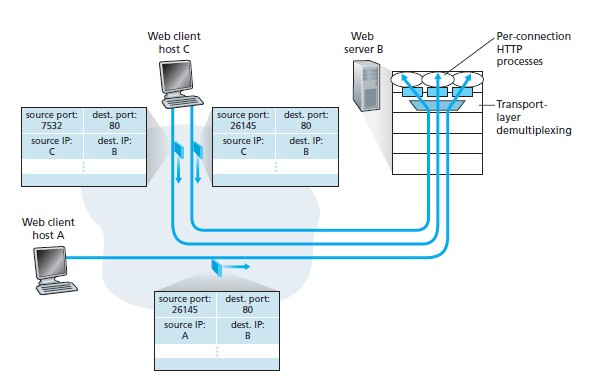
\includegraphics[width=0.6\linewidth]{cap08/demux_http.png}
    \caption{Due client (A e C) aprono tre connessioni HTTP verso il server B: i segmenti sono smistati usando la quaterna completa.}
\end{figure}

\begin{itemize}
    \item L'host C apre \textbf{due} sessioni HTTP verso il server B e l'host A ne apre \textbf{una}. A, C e B hanno
          indirizzi IP distinti.
    \item C assegna alle sue due connessioni porte sorgente diverse (26145 e 7532).
    \item A, che non sa nulla di C, potrebbe scegliere anch'esso la porta 26145: nessun problema, perché le due
          connessioni hanno \textbf{indirizzi IP sorgente diversi}.
    \item Il server apre un nuovo processo (o thread) per ogni connessione, con il suo socket dedicato. È
          l'approccio tipico, ma aprire troppi processi o thread può peggiorare le prestazioni del server.
\end{itemize}

\begin{table}[H]
\centering
\begin{tabular}{llllc}
\toprule
\textbf{IP sorgente} & \textbf{porta sorgente} & \textbf{IP destinazione} & \textbf{porta dest.} & \textbf{socket} \\
\midrule
C & 26145 & B & 80 & 1 \\
C & 7532 & B & 80 & 2 \\
A & 26145 & B & 80 & 3 \\
\bottomrule
\end{tabular}
\caption{Tre connessioni verso la stessa porta 80 del server: le quaterne sono tutte diverse.}
\end{table}

% ══════════════════════════════════════════════════════════════
\section{UDP}
% ══════════════════════════════════════════════════════════════

\dfn{UDP (User Datagram Protocol)}{
    UDP è il protocollo di trasporto \textbf{minimale}: aggiunge a IP ``solo l'essenziale'', cioè
    \begin{itemize}
      \item la \textbf{consegna processo-a-processo} (porte, multiplexing e demultiplexing);
      \item il \textbf{controllo degli errori} (checksum).
    \end{itemize}
    È \textbf{senza connessione} (nessun handshake prima di inviare), \textbf{non garantisce la consegna} e
    \textbf{non ha controllo di flusso né di congestione}.
}

\subsection{Perché usare UDP invece di TCP}

\begin{itemize}
    \item \textbf{Controllo a livello applicativo}: UDP è più diretto, e l'applicazione controlla meglio
          \emph{cosa} e \emph{quando} viene inviato. Utile nelle applicazioni in tempo reale, dove velocità di
          invio e ritardi contano più di qualche dato perso.
    \item \textbf{Nessun ritardo di connessione}: niente handshake, quindi niente attesa prima di trasmettere.
          Ottimo per il DNS, che non deve aggiungere ritardi a ogni navigazione.
    \item \textbf{Nessuno stato della connessione}: niente buffer, parametri di congestione, numeri di sequenza e di
          ack da mantenere. Un server UDP può gestire molti più client attivi di uno TCP.
    \item \textbf{Header piccolo}: TCP aggiunge 20 byte di header a ogni segmento, UDP solo \textbf{8}.
\end{itemize}

\begin{esempio}{Il DNS su UDP}
\begin{itemize}
    \item \textbf{Livello applicativo}: l'host che vuole interrogare un server DNS costruisce un messaggio di
          richiesta e lo passa a UDP.
    \item \textbf{Livello di trasporto}: senza alcun handshake, UDP aggiunge l'header e passa il segmento al
          livello di rete.
    \item \textbf{Livello di rete}: il segmento UDP viene incapsulato in un datagramma IP e inviato al server DNS.
\end{itemize}
Il client poi attende la risposta. Se non arriva (magari la rete ha perso la domanda o la risposta), può
\textbf{rinviare} la richiesta, \textbf{chiedere a un altro} name server, oppure \textbf{avvisare} l'applicazione
che la risposta non è arrivata. L'affidabilità, se serve, la gestisce l'applicazione.
\end{esempio}

\subsection{Chi usa cosa}

\begin{table}[H]
\centering
\begin{tabular}{lll}
\toprule
\textbf{Servizio} & \textbf{Protocollo applicativo} & \textbf{Trasporto} \\
\midrule
Posta elettronica & SMTP & TCP \\
Terminale remoto & Telnet, SSH & TCP \\
Web & HTTP & TCP (o UDP con HTTP/3) \\
Trasferimento file & FTP & TCP \\
Traduzione dei nomi & DNS & UDP \\
Gestione dei dispositivi di rete & SNMP & UDP \\
Streaming multimediale & proprietario & UDP o TCP \\
Telefonia su Internet & proprietario & UDP o TCP \\
\bottomrule
\end{tabular}
\caption{Applicazioni e protocolli di trasporto.}
\end{table}

\begin{itemize}
    \item Chi ha bisogno di \textbf{affidabilità} (posta, terminale remoto, Web) usa TCP, oppure protocolli
          affidabili costruiti su UDP come QUIC: una mail non può arrivare a pezzi.
    \item \textbf{SNMP} usa UDP perché le applicazioni di gestione devono funzionare proprio quando la rete è in
          difficoltà, e il trasferimento affidabile con tutti i suoi controlli sarebbe difficile.
    \item Le applicazioni \textbf{multimediali} (telefonia, videoconferenza, streaming) usano spesso UDP: tollerano
          qualche perdita e reagiscono male al controllo di congestione di TCP.
\end{itemize}

\warning{Il lato oscuro di UDP}{
    Usare UDP per le applicazioni multimediali è \textbf{controverso}, proprio perché non c'è controllo di
    congestione. Se tutti inviassero egoisticamente video ad alta velocità senza alcun controllo, i router
    traboccherebbero, facendo perdere ancora più pacchetti UDP. E le perdite elevate spingerebbero i
    mittenti TCP, che invece si controllano, a ridurre drasticamente la loro velocità.
}

% ══════════════════════════════════════════════════════════════
\section{Il formato del segmento UDP}
% ══════════════════════════════════════════════════════════════

\begin{figure}[H]
\centering
\begin{tikzpicture}[every node/.style={font=\small\sffamily}]
  \node[field, fill=ltra, minimum width=4cm, minimum height=0.8cm] (sp) at (0,0) {porta sorgente};
  \node[field, fill=ltra, minimum width=4cm, minimum height=0.8cm, right=0pt of sp] (dp) {porta destinazione};
  \node[field, fill=ltra!60, minimum width=4cm, minimum height=0.8cm, below=0pt of sp] (ln) {lunghezza};
  \node[field, fill=ltra!60, minimum width=4cm, minimum height=0.8cm, below=0pt of dp] (ck) {checksum};
  \node[field, fill=lapp!60, minimum width=8cm, minimum height=1.6cm, anchor=north west] (d) at (ln.south west) {dati dell'applicazione (messaggio)};
  \draw[{Stealth}-{Stealth}] ([yshift=0.3cm]sp.north west) -- node[above, font=\scriptsize\sffamily] {32 bit} ([yshift=0.3cm]dp.north east);
  \draw[{Stealth}-{Stealth}] ([yshift=0.1cm]sp.north west) -- node[below, font=\scriptsize\sffamily, fill=white, inner sep=1pt] {16 bit} ([yshift=0.1cm]sp.north east);
  \draw[decorate, decoration={brace, amplitude=5pt}] ([xshift=0.2cm]dp.north east) -- ([xshift=0.2cm]ck.south east) node[midway, right=6pt, font=\scriptsize\sffamily] {header: 8 byte};
  \draw[decorate, decoration={brace, amplitude=5pt}] ([xshift=0.2cm]ck.south east) -- ([xshift=0.2cm]d.south east) node[midway, right=6pt, font=\scriptsize\sffamily] {dati: lunghezza variabile};
\end{tikzpicture}
\caption{Il segmento (datagramma) UDP.}
\end{figure}

L'header UDP è lungo \textbf{8 byte} (64 bit) e ha quattro campi da 16 bit:

\begin{itemize}
    \item \textbf{porta sorgente}: la porta del processo mittente;
    \item \textbf{porta di destinazione}: la porta del processo destinatario;
    \item \textbf{lunghezza}: la lunghezza, in byte, dell'intero datagramma (header + dati);
    \item \textbf{checksum}: usata dal destinatario per controllare che il messaggio sia integro.
\end{itemize}

Seguono i \textbf{dati}, cioè il messaggio del livello applicativo.

% ══════════════════════════════════════════════════════════════
\section{Il checksum UDP}
% ══════════════════════════════════════════════════════════════

\dfn{Checksum}{
    Il \textbf{checksum} UDP è un campo di 16 bit per la rilevazione degli errori.
    \begin{itemize}
      \item \textbf{Mittente}: somma tutte le parole da 16 bit del datagramma, riportando ogni bit di overflow
            (\emph{wraparound}) nella somma, e calcola il \textbf{complemento a 1} del risultato (inverte tutti i
            bit). Il risultato va nel campo checksum.
      \item \textbf{Destinatario}: somma tutte le parole da 16 bit ricevute, \textbf{checksum compresa}. Se non ci
            sono errori il risultato è \texttt{1111111111111111} (sedici 1). Se anche un solo bit è 0, il
            pacchetto contiene errori.
    \end{itemize}
}

\begin{esempio}{Calcolo del checksum su tre parole}
\begin{center}
\begin{tabular}{rl}
      & \texttt{0110011001100000} \quad (prima parola) \\
$+$   & \texttt{0101010101010101} \quad (seconda parola) \\
\midrule
      & \texttt{1011101110110101} \quad (somma delle prime due) \\
$+$   & \texttt{1000111100001100} \quad (terza parola) \\
\midrule
      & \texttt{\textcolor{netred}{1}0100101011000001} \quad (c'è un bit di overflow) \\
$+$   & \texttt{0000000000000001} \quad (wraparound: si somma il riporto) \\
\midrule
      & \texttt{0100101011000010} \quad (somma) \\
\midrule
checksum $=$ & \texttt{\textbf{1011010100111101}} \quad (complemento a 1: si invertono i bit) \\
\end{tabular}
\end{center}
Al destinatario: $\texttt{0100101011000010} + \texttt{1011010100111101} = \texttt{1111111111111111}$, quindi
nessun errore rilevato.
\end{esempio}

\info{Perché il checksum, se c'è già il livello di collegamento?}{
    Molti protocolli di collegamento controllano già gli errori, ma non è garantito che lo facciano
    \textbf{tutti} i collegamenti del cammino, e un errore può anche nascere mentre un segmento è nella
    memoria di un router. Poiché il trasporto deve funzionare da un estremo all'altro, controllare
    l'integrità \textbf{end-to-end} è necessario (principio \emph{end-to-end}). Per rendere il controllo più
    robusto, il checksum viene calcolato anche su alcuni campi dell'header IP (gli indirizzi, il cosiddetto
    \emph{pseudo-header}).
}

\warning{Rilevare non è correggere}{
    Il checksum \textbf{rileva} alcuni errori ma non li \textbf{corregge}, e non li rileva tutti: se due bit si
    invertono in modo che le somme si compensino, l'errore passa inosservato. Cosa fare di un segmento
    danneggiato UDP non lo dice: di solito lo scarta, oppure lo passa all'applicazione con un avviso.
}

% ══════════════════════════════════════════════════════════════
\section{Riepilogo}
% ══════════════════════════════════════════════════════════════

\riepilogo{
\begin{itemize}
    \item Il trasporto offre comunicazione logica \textbf{tra processi}; la rete, \textbf{tra host}.
    \item Quattro servizi: consegna processo-a-processo, integrità, affidabilità, controllo di flusso e congestione;
          UDP fa i primi due, TCP tutti.
    \item Le \textbf{porte} (16 bit) identificano i socket; multiplexing al mittente, demultiplexing al destinatario.
    \item Socket UDP: identificato da (IP dest, porta dest). Socket TCP: dalla \textbf{quaterna} completa.
    \item \textbf{UDP}: senza connessione, header di 8 byte (porte, lunghezza, checksum), nessuna garanzia; usato da
          DNS, SNMP, applicazioni multimediali.
    \item Il \textbf{checksum} è il complemento a 1 della somma a 16 bit con wraparound.
\end{itemize}
}
     % Trasporto e UDP
  \chapter{Il trasferimento dati affidabile}

% ══════════════════════════════════════════════════════════════
\section{Il problema}
% ══════════════════════════════════════════════════════════════

Siamo in stazione ad aspettare il treno numero 6, previsto al binario 5. Il treno cambia binario e
arriverà al 9: la stazione lo comunica con un messaggio, ``\emph{Il treno 6 arriverà al binario 9}''.
Cosa succede se la comunicazione è inaffidabile?

\begin{itemize}
    \item le parole possono \textbf{perdersi}: ``\emph{Il treno \%\&! arriverà al binario 9}'';
    \item possono essere \textbf{alterate}: ``\emph{Il treno 7 arriverà al binario 9}'';
    \item possono essere \textbf{scambiate}: ``\emph{Il treno 9 arriverà al binario 6}'';
    \item possono essere \textbf{duplicate}: ``\emph{Il treno 66 arriverà al binario 9}''.
\end{itemize}

Nel primo caso ci si accorge che il messaggio è sbagliato; negli altri si rischia di prendere il treno
sbagliato o di perdere quello giusto.

Il controllo degli errori (per esempio con il checksum) permette al destinatario almeno di capire se un
messaggio è corrotto, ma non basta. Il trasferimento affidabile è uno dei problemi centrali delle reti, e
non viene affrontato solo dal trasporto, ma anche dal livello di collegamento e spesso da quello applicativo.

\dfn{Canale affidabile}{
    In un canale affidabile sono garantite tre cose:
    \begin{enumerate}
      \item nessun bit trasmesso viene \textbf{corrotto} (da 0 a 1 o viceversa);
      \item nessun bit viene \textbf{perso} o \textbf{duplicato};
      \item tutti i bit arrivano \textbf{nell'ordine} in cui sono stati inviati.
    \end{enumerate}
}

\warning{Si parte da un canale inaffidabile}{
    In generale si deve assumere che il livello di rete sottostante sia \textbf{inaffidabile}. È un'ipotesi
    realistica: TCP è un protocollo affidabile costruito sopra IP, che è inaffidabile. Studieremo il problema
    complicando il canale un passo alla volta: prima solo bit corrotti, poi anche pacchetti persi.
}

\begin{figure}[H]
\centering
\begin{tikzpicture}[every node/.style={font=\footnotesize\sffamily}]
  \node[lay app, minimum width=3cm] (sa) at (0,1.2) {processo mittente};
  \node[lay app, minimum width=3cm] (ra) at (8,1.2) {processo ricevente};
  \node[draw, fill=ltra, minimum width=3cm, minimum height=0.9cm, align=center] (st) at (0,0) {protocollo di trasferimento\\affidabile (mittente)};
  \node[draw, fill=ltra, minimum width=3cm, minimum height=0.9cm, align=center] (rt) at (8,0) {protocollo di trasferimento\\affidabile (ricevente)};
  \draw[-{Stealth}, thick] (sa) -- (st); \draw[-{Stealth}, thick] (rt) -- (ra);
  \draw[{Stealth}-{Stealth}, very thick, netred, decorate, decoration={snake, amplitude=1.5pt, segment length=8pt, pre length=3pt, post length=3pt}] (st) -- node[above=3pt] {canale inaffidabile} node[below=3pt, text=netred] {bit corrotti, pacchetti persi} (rt);
  \draw[dashed, primary, thick] (sa.east) -- node[above] {servizio offerto: canale affidabile} (ra.west);
\end{tikzpicture}
\caption{Il protocollo di trasferimento affidabile offre all'applicazione un canale affidabile, costruendolo sopra un canale che non lo è.}
\end{figure}

% ══════════════════════════════════════════════════════════════
\section{Stop-and-wait con corruzione dei pacchetti}
% ══════════════════════════════════════════════════════════════

Supponiamo che il canale possa solo \textbf{corrompere} i bit, senza perdere pacchetti. La corruzione è un
problema tipico, dovuto soprattutto alle componenti fisiche: un pacchetto viene trasmesso, propagato,
memorizzato in buffer molte volte durante il viaggio.

\dfn{Stop-and-wait}{
    Nel protocollo \textbf{stop-and-wait} il mittente invia un messaggio e \textbf{aspetta una conferma} prima
    di inviarne un altro:
    \begin{itemize}
      \item un \textbf{ACK} (\emph{acknowledgment} positivo) significa che il messaggio è arrivato integro;
      \item un \textbf{NAK} (\emph{acknowledgment} negativo) significa che c'è stato un errore e il messaggio va ripetuto.
    \end{itemize}
    I protocolli basati sulla ritrasmissione si chiamano \textbf{ARQ} (\emph{Automatic Repeat reQuest}).
}

\begin{figure}[H]
\centering
\begin{tikzpicture}[yscale=0.85, every node/.style={font=\footnotesize\sffamily}]
  \timeline{a}{0}{Host A}{5.6}
  \timeline{b}{6}{Host B}{5.6}
  \draw[msg] (0,-0.3) -- node[above, sloped] {``Treno''} (6,-1.0);
  \draw[msg, netgreen] (6,-1.2) -- node[above, sloped] {ACK} (0,-1.9);
  \draw[msg] (0,-2.1) -- node[above, sloped] {``6''} (6,-2.8);
  \node[text=netred, anchor=west] at (6.2,-2.8) {checksum errato: corrotto!};
  \draw[msg, netred] (6,-3.0) -- node[above, sloped] {NAK} (0,-3.7);
  \draw[msg] (0,-3.9) -- node[above, sloped] {``6'' (ritrasmesso)} (6,-4.6);
  \draw[msg, netgreen] (6,-4.8) -- node[above, sloped] {ACK} (0,-5.5);
\end{tikzpicture}
\caption{Stop-and-wait con conferme positive e negative.}
\end{figure}

\subsection{I due problemi dello stop-and-wait ingenuo}

\begin{itemize}
    \item Che succede se è \textbf{l'ACK o il NAK a essere corrotto}? Il mittente non sa cosa sia successo al suo messaggio.
    \item Se il mittente, nel dubbio, ritrasmette, come fa B a sapere se il messaggio è una \textbf{ripetizione} o un
          \textbf{messaggio nuovo}?
\end{itemize}

\dfn{Numero di sequenza}{
    Si aggiunge all'header dei pacchetti un campo, il \textbf{numero di sequenza}, che indica l'ordine dei
    pacchetti. Il ricevente può così riconoscere e scartare i duplicati.
}

In stop-and-wait c'è \textbf{un solo messaggio alla volta} sulla linea: non serve numerare l'intera
sequenza, basta distinguere il pacchetto attuale dal precedente. È sufficiente \textbf{un bit}
($s = 0$ oppure $s = 1$).

\begin{figure}[H]
\centering
\begin{tikzpicture}[yscale=0.85, every node/.style={font=\footnotesize\sffamily}]
  \timeline{a}{0}{Host A}{5.6}
  \timeline{b}{6}{Host B}{5.6}
  \draw[msg] (0,-0.3) -- node[above, sloped] {``Treno'' [$s=0$]} (6,-1.0);
  \draw[msg, netgreen] (6,-1.2) -- node[above, sloped] {ACK [$s=0$]} (0,-1.9);
  \draw[msg] (0,-2.1) -- node[above, sloped] {``6'' [$s=1$]} (6,-2.8);
  \node[text=netred, anchor=west] at (6.2,-2.8) {corrotto};
  \draw[msg, netred] (6,-3.0) -- node[above, sloped] {NAK [$s=1$]} (0,-3.7);
  \draw[msg] (0,-3.9) -- node[above, sloped] {``6'' [$s=1$]} (6,-4.6);
  \node[anchor=west, text width=4.5cm, align=left] at (6.2,-4.6) {$s=1$ di nuovo: è la \textbf{ritrasmissione} del messaggio precedente, non uno nuovo};
  \draw[msg, netgreen] (6,-4.8) -- node[above, sloped] {ACK [$s=1$]} (0,-5.5);
\end{tikzpicture}
\caption{Con un bit di sequenza il ricevente distingue un messaggio nuovo da una ritrasmissione.}
\end{figure}

% ══════════════════════════════════════════════════════════════
\section{Stop-and-wait con perdita dei pacchetti}
% ══════════════════════════════════════════════════════════════

Ora il canale può anche \textbf{perdere} pacchetti. È realistico: i dispositivi di rete possono avere i
buffer pieni quando il traffico è intenso.

Con lo stop-and-wait visto finora c'è un problema evidente: il \textbf{blocco}. Se un messaggio si perde,
il mittente aspetta per sempre un ACK che non arriverà, e nessuno invia più nulla. Succede sia se si perde
il messaggio sia se si perde l'ACK: in entrambi i casi A non riceve lo stimolo per inviare di nuovo.

\dfn{Timeout}{
    Il mittente fa partire un \textbf{timer} a ogni invio. Se il timer scade (\textbf{timeout}) prima che
    arrivi la conferma, il mittente \textbf{ritrasmette} il messaggio. Il meccanismo funziona sia quando si
    perde il pacchetto sia quando si perde l'ACK; un approccio simile si usa nel DNS su UDP.
}

\begin{figure}[H]
\centering
\begin{tikzpicture}[yscale=0.8, every node/.style={font=\scriptsize\sffamily}]
  \begin{scope}
    \node[font=\footnotesize\bfseries\sffamily] at (1.75,1.1) {(a) si perde il pacchetto};
    \timeline{a}{0}{A}{5.5}
    \timeline{b}{3.5}{B}{5.5}
    \draw[msg] (0,-0.3) -- node[above, sloped] {pkt [$s=0$]} (3.5,-1.0);
    \draw[msg, netgreen] (3.5,-1.2) -- node[above, sloped] {ACK 0} (0,-1.9);
    \draw[msglost] (0,-2.1) -- (2.0,-2.5); \node[text=netred] at (2.4,-2.2) {persa};
    \draw[netorange, thick] (-0.25,-2.1) -- (-0.25,-4.0); \node[text=netorange, rotate=90] at (-0.5,-3.05) {timeout};
    \draw[msg] (0,-4.0) -- node[above, sloped] {pkt [$s=1$]} (3.5,-4.7);
    \draw[msg, netgreen] (3.5,-4.9) -- node[above, sloped] {ACK 1} (0,-5.5);
  \end{scope}
  \begin{scope}[xshift=5.2cm]
    \node[font=\footnotesize\bfseries\sffamily] at (1.75,1.1) {(b) si perde l'ACK};
    \timeline{a}{0}{A}{5.5}
    \timeline{b}{3.5}{B}{5.5}
    \draw[msg] (0,-0.3) -- node[above, sloped] {pkt [$s=0$]} (3.5,-1.0);
    \draw[msglost] (3.5,-1.2) -- (1.6,-1.6); \node[text=netred] at (1.2,-1.3) {perso};
    \draw[netorange, thick] (-0.25,-0.3) -- (-0.25,-2.6); \node[text=netorange, rotate=90] at (-0.5,-1.45) {timeout};
    \draw[msg] (0,-2.6) -- node[above, sloped] {pkt [$s=0$]} (3.5,-3.3);
    \node[anchor=west, text width=1.8cm, align=left, text=netblue] at (3.6,-3.3) {duplicato: scartato, ma ri-inviato l'ACK};
    \draw[msg, netgreen] (3.5,-3.8) -- node[above, sloped] {ACK 0} (0,-4.5);
  \end{scope}
  \begin{scope}[xshift=10.8cm]
    \node[font=\footnotesize\bfseries\sffamily] at (1.75,1.1) {(c) timeout troppo breve};
    \timeline{a}{0}{A}{5.5}
    \timeline{b}{3.5}{B}{5.5}
    \draw[msg] (0,-0.3) -- node[above, sloped] {M1 [$s=0$]} (3.5,-1.3);
    \draw[netorange, thick] (-0.25,-0.3) -- (-0.25,-1.6); \node[text=netorange, rotate=90] at (-0.5,-0.95) {timeout};
    \draw[msg, netgreen] (3.5,-1.5) -- node[above, sloped] {ACK 0} (0,-2.5);
    \draw[msg, netred] (0,-1.6) -- node[below, sloped] {M1 [$s=0$] di nuovo} (3.5,-2.6);
    \node[anchor=north, text width=3.6cm, align=center, text=netred] at (1.75,-3.1) {il timeout è minore dell'RTT: A ritrasmette M1 anche se messaggio e ACK non si sono persi};
  \end{scope}
\end{tikzpicture}
\caption{Il timeout salva lo stop-and-wait dal blocco. In caso di duplicato il ricevente scarta il pacchetto ma deve rimandare l'ACK.}
\end{figure}

\subsection{La stima del timeout}

La difficoltà è scegliere un timeout adatto, e questo dipende dall'\textbf{RTT}:

\begin{itemize}
    \item un timeout \textbf{troppo lungo} rallenta la comunicazione (dopo una perdita si aspetta a vuoto);
    \item un timeout \textbf{troppo breve} fa sovrapporre i pacchetti, con ritrasmissioni inutili (caso (c) della figura).
\end{itemize}

Un timeout ragionevole deve essere \textbf{un po' più lungo dell'RTT}. Il timeout salva lo stop-and-wait dal
blocco, ma le \textbf{prestazioni} restano pessime, come vediamo ora.

% ══════════════════════════════════════════════════════════════
\section{Il modello “ad acqua”}
% ══════════════════════════════════════════════════════════════

Per ragionare sui tempi si può immaginare la trasmissione come acqua che passa da un serbatoio a un altro
attraverso un tubo.

\begin{figure}[H]
\centering
\begin{tikzpicture}[every node/.style={font=\footnotesize\sffamily}]
  % fase 1
  \begin{scope}
    \draw[thick] (0,0) rectangle (1,1.6); \fill[netblue!50] (0.02,0.02) rectangle (0.98,0.8);
    \draw[thick] (1,0.2) -- (3.4,0.2); \draw[thick] (1,0.5) -- (3.4,0.5); \fill[netblue!50] (1,0.22) rectangle (1.9,0.48);
    \draw[thick] (3.4,0) rectangle (4.4,1.6);
    \node at (2.2,-0.5) {1. si svuota il serbatoio: tempo $t$};
  \end{scope}
  \begin{scope}[yshift=-2.6cm]
    \draw[thick] (0,0) rectangle (1,1.6);
    \draw[thick] (1,0.2) -- (3.4,0.2); \draw[thick] (1,0.5) -- (3.4,0.5); \fill[netblue!50] (1.4,0.22) rectangle (3.0,0.48);
    \draw[thick] (3.4,0) rectangle (4.4,1.6);
    \node at (2.2,-0.5) {2. l'acqua scorre nel tubo: $\text{RTT}/2$};
  \end{scope}
  \begin{scope}[yshift=-5.2cm]
    \draw[thick] (0,0) rectangle (1,1.6);
    \draw[thick] (1,0.2) -- (3.4,0.2); \draw[thick] (1,0.5) -- (3.4,0.5); \fill[netblue!50] (2.6,0.22) rectangle (3.4,0.48);
    \draw[thick] (3.4,0) rectangle (4.4,1.6); \fill[netblue!50] (3.42,0.02) rectangle (4.38,0.8);
    \node at (2.2,-0.5) {3. si riempie il serbatoio di arrivo: tempo $t$};
  \end{scope}
  \node[draw, fill=cloudbg, rounded corners, text width=6.8cm, align=left, anchor=west] at (5.6,-2.2) {
    \begin{itemize}\setlength\itemsep{1pt}
      \item $t$ = tempo per ``versare'' tutti i bit nel collegamento (tempo di trasmissione, $L/R$);
      \item $\text{RTT}/2$ = tempo di propagazione fino al destinatario;
      \item l'ultima goccia arriva dopo $\text{RTT}/2 + t$ dall'inizio.
    \end{itemize}
    \textbf{Tempo totale} $= \text{RTT}/2 + t$
  };
\end{tikzpicture}
\caption{Il trasferimento come flusso d'acqua: mentre il serbatoio si svuota l'acqua già si muove nel tubo, e l'ultima goccia arriva dopo $\text{RTT}/2 + t$.}
\end{figure}

% ══════════════════════════════════════════════════════════════
\section{Le prestazioni dello stop-and-wait}
% ══════════════════════════════════════════════════════════════

Consideriamo il caso ideale di due host sulle coste opposte degli Stati Uniti. L'RTT alla velocità della
luce è di circa \textbf{30 ms} (0,03 s). Supponiamo:

\begin{itemize}
    \item un canale con \textbf{velocità di trasmissione} $R = 1$ Gb/s $= 10^9$ bit/s;
    \item pacchetti di \textbf{dimensione} $L = 1000$ byte $= 8000$ bit.
\end{itemize}

Il tempo per immettere il pacchetto nel canale è:
$$t = \frac{L}{R} = \frac{8000\ \text{bit}}{10^9\ \text{bit/s}} = 8\cdot 10^{-6}\ \text{s} = 8\ \mu\text{s}$$

In stop-and-wait:

\begin{itemize}
    \item il mittente comincia a trasmettere al tempo $t_0$;
    \item l'ultimo bit entra nel canale a $t_0 + 0{,}000008$ s;
    \item il pacchetto impiega $0{,}015$ s per arrivare;
    \item l'ultimo bit arriva a $t = \text{RTT}/2 + L/R = 0{,}015008$ s;
    \item supponendo gli ACK piccolissimi (tempo di trasmissione trascurabile), l'ACK torna al mittente a
          $t = \text{RTT} + L/R = 0{,}030008$ s.
\end{itemize}

\dfn{Utilizzo del mittente}{
    L'\textbf{utilizzo} è la frazione di tempo in cui il mittente è effettivamente occupato a trasmettere:
    $$U_{\text{mittente}} = \frac{L/R}{\text{RTT} + L/R} = \frac{0{,}000008}{0{,}030008} \approx 0{,}00027$$
}

Su 0,030008 s di tempo complessivo, il mittente ha trasmesso solo lo 0,027\% del tempo: è rimasto
\textbf{in attesa il 99,973\% del tempo}. Un collegamento da 1 Gb/s usato così trasmette in media
circa 267 kb/s!

% ══════════════════════════════════════════════════════════════
\section{Il pipelining}
% ══════════════════════════════════════════════════════════════

\dfn{Pipelining}{
    Con il \textbf{pipelining} il mittente può inviare \textbf{più pacchetti} senza aspettare le conferme.
}

\begin{figure}[H]
\centering
\begin{tikzpicture}[yscale=0.8, every node/.style={font=\scriptsize\sffamily}]
  \begin{scope}
    \node[font=\footnotesize\bfseries\sffamily] at (1.8,1.1) {Stop-and-wait};
    \timeline{a}{0}{mittente}{4.3}
    \timeline{b}{3.6}{ricevente}{4.3}
    \fill[netblue!40] (0,0) -- (3.6,-1.5) -- (3.6,-1.7) -- (0,-0.2) -- cycle;
    \draw[msg, netgreen] (3.6,-1.7) -- node[above, sloped] {ACK} (0,-3.2);
    \fill[netblue!40] (0,-3.2) -- (3.6,-4.7) -- (3.6,-4.9) -- (0,-3.4) -- cycle;
  \end{scope}
  \begin{scope}[xshift=7cm]
    \node[font=\footnotesize\bfseries\sffamily] at (1.8,1.1) {Pipelining (3 pacchetti)};
    \timeline{a}{0}{mittente}{4.3}
    \timeline{b}{3.6}{ricevente}{4.3}
    \foreach \k in {0,1,2} \fill[netblue!40] (0,-\k*0.25) -- (3.6,-1.5-\k*0.25) -- (3.6,-1.7-\k*0.25) -- (0,-0.2-\k*0.25) -- cycle;
    \foreach \k in {0,1,2} \draw[msg, netgreen] (3.6,-1.7-\k*0.25) -- (0,-3.2-\k*0.25);
    \node[text=netgreen!60!black] at (1.8,-3.9) {3 ACK};
    \foreach \k in {0,1,2} \fill[netblue!40] (0,-3.2-\k*0.25) -- (3.6,-4.7-\k*0.25) -- (3.6,-4.9-\k*0.25) -- (0,-3.4-\k*0.25) -- cycle;
  \end{scope}
\end{tikzpicture}
\caption{Nello stesso tempo il pipelining trasmette più pacchetti: l'utilizzo cresce (quasi) in proporzione.}
\end{figure}

Con 3 pacchetti invece di uno: l'ultimo bit dell'ultimo pacchetto entra nel canale a $t_0 + 0{,}000024$ s,
arriva a $0{,}015024$ s e l'ACK torna a $0{,}030024$ s. Il mittente ha lavorato tre volte tanto:
$$U = \frac{3\cdot L/R}{\text{RTT} + L/R} = \frac{0{,}000024}{0{,}030008} \approx 0{,}0008$$
cioè ha aspettato il 99,92\% del tempo invece del 99,973\%. Il guadagno cresce con il numero di pacchetti
inviati in parallelo.

Il pipelining ha però delle conseguenze:

\begin{itemize}
    \item l'intervallo dei \textbf{numeri di sequenza} deve crescere: ogni pacchetto in viaggio (escluse le
          ritrasmissioni) deve avere un numero univoco, e ci possono essere più pacchetti in viaggio non ancora confermati;
    \item servono dei \textbf{buffer} per conservare i pacchetti, sia al mittente (quelli inviati ma non
          confermati) sia eventualmente al ricevente (non sappiamo se ci sono ``buchi'' nella trasmissione).
\end{itemize}

I due protocolli fondamentali basati sul pipelining sono \textbf{Go-Back-N} e \textbf{Selective Repeat}.

% ══════════════════════════════════════════════════════════════
\section{Go-Back-N}
% ══════════════════════════════════════════════════════════════

\dfn{Go-Back-N (GBN)}{
    Nel protocollo \textbf{Go-Back-N} (detto anche protocollo a \emph{finestra scorrevole}) il mittente può
    trasmettere più pacchetti senza aspettare le conferme, ma può avere \textbf{al massimo $N$ pacchetti
    non confermati} contemporaneamente.
}

\begin{figure}[H]
    \centering
    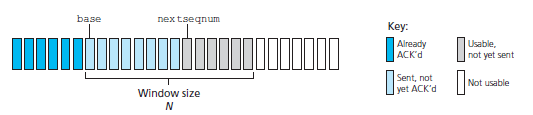
\includegraphics[width=0.62\linewidth]{cap09/gbn_finestra.png}
    \caption{La finestra del mittente in Go-Back-N: blu i pacchetti già confermati, azzurri quelli inviati e non confermati, bianchi quelli utilizzabili, grigi quelli non ancora utilizzabili.}
\end{figure}

Il mittente mantiene due indici:

\begin{itemize}
    \item \texttt{base}: il numero di sequenza del \textbf{più vecchio pacchetto non confermato};
    \item \texttt{nextseqnum}: il più piccolo numero di sequenza \textbf{non ancora usato} (il prossimo da inviare).
\end{itemize}

\begin{table}[H]
\centering
\begin{tabular}{ll}
\toprule
\textbf{Intervallo} & \textbf{Stato dei pacchetti} \\
\midrule
$[0,\ \texttt{base}-1]$ & trasmessi e confermati \\
$[\texttt{base},\ \texttt{nextseqnum}-1]$ & inviati ma non ancora confermati \\
$[\texttt{nextseqnum},\ \texttt{base}+N-1]$ & possono essere inviati \\
$[\texttt{base}+N,\ +\infty)$ & non utilizzabili finché non arriva una nuova conferma \\
\bottomrule
\end{tabular}
\caption{Le zone della finestra di Go-Back-N ($N$ è la dimensione della finestra).}
\end{table}

Quando arriva la conferma di \texttt{base}, la finestra \textbf{scorre} in avanti. In GBN gli ACK sono
\textbf{cumulativi}: ``ACK $n$'' significa ``ho ricevuto correttamente tutto fino a $n$ compreso''. C'è un
unico timer, per il pacchetto più vecchio non confermato; se scade, il mittente \textbf{ritrasmette tutti i
pacchetti inviati e non confermati}: da qui il nome ``torna indietro di $N$''.

\subsection{Il ricevente in GBN}

Il ricevente di GBN è molto semplice:

\begin{itemize}
    \item \textbf{scarta i pacchetti fuori ordine}, anche se sono integri;
    \item consegna all'applicazione solo i pacchetti \textbf{in ordine}, e conferma l'ultimo ricevuto in ordine;
    \item i pacchetti scartati (non confermati) verranno prima o poi ritrasmessi dal mittente.
\end{itemize}

Si buttano via anche pacchetti buoni, ma il processo resta semplice: il mittente mantiene gli indici della
finestra, il ricevente solo il numero di sequenza del prossimo pacchetto atteso.

\begin{figure}[H]
\centering
\begin{minipage}{0.4\linewidth}\centering
  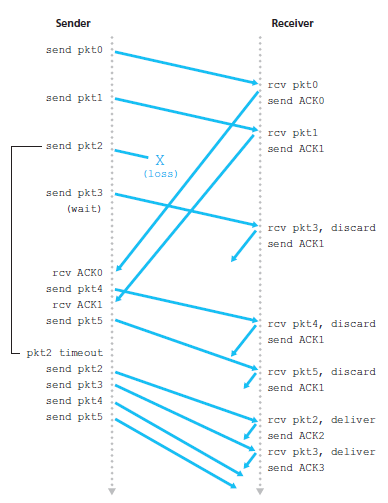
\includegraphics[width=0.9\linewidth]{cap09/gbn_esempio.png}
\end{minipage}\hfill
\begin{minipage}{0.56\linewidth}
Finestra di dimensione $N=4$; il pacchetto 2 si perde.
\begin{itemize}
  \item Il ricevente riceve 0 e 1 e li conferma.
  \item Arrivano 3, 4 e 5: sono \textbf{fuori ordine} (manca il 2), quindi vengono \textbf{scartati}, e per ciascuno
        il ricevente rimanda ACK~1 (l'ultimo ricevuto in ordine).
  \item Al mittente scade il timer del pacchetto 2: ritrasmette 2, 3, 4 e 5.
\end{itemize}
\end{minipage}
\caption{Go-Back-N in azione: poiché si perde pkt2, anche pkt3, pkt4 e pkt5 vanno scartati e ritrasmessi, pur essendo arrivati integri.}
\end{figure}

\warning{Una reazione a catena}{
    Lo svantaggio di scartare pacchetti ricevuti correttamente è che bisogna \textbf{rispedirli}. È una reazione a
    catena: se si perdono pacchetti per problemi di rete, molti pacchetti buoni ma fuori ordine vengono buttati,
    costringendo il mittente a ritrasmetterli; e le ritrasmissioni stesse possono perdersi o danneggiarsi,
    richiedendo ancora altre ritrasmissioni.
}

% ══════════════════════════════════════════════════════════════
\section{Selective Repeat}
% ══════════════════════════════════════════════════════════════

Anche se GBN è molto meglio dello stop-and-wait, con finestre grandi un solo errore può causare la
ritrasmissione di moltissimi pacchetti, per lo più inutilmente.

\dfn{Selective Repeat (SR)}{
    Nel protocollo \textbf{Selective Repeat} il mittente \textbf{ritrasmette solo i pacchetti che
    probabilmente sono andati persi o corrotti}:
    \begin{itemize}
      \item come in GBN, si usa una finestra di dimensione $N$ per limitare i pacchetti non confermati;
      \item a differenza di GBN, ogni pacchetto è \textbf{confermato singolarmente} (ACK non cumulativi) e ha
            il \textbf{proprio timer};
      \item il ricevente \textbf{conserva in un buffer} e conferma anche i pacchetti fuori ordine, e li consegna
            all'applicazione quando i ``buchi'' sono stati colmati.
    \end{itemize}
}

\begin{figure}[H]
    \centering
    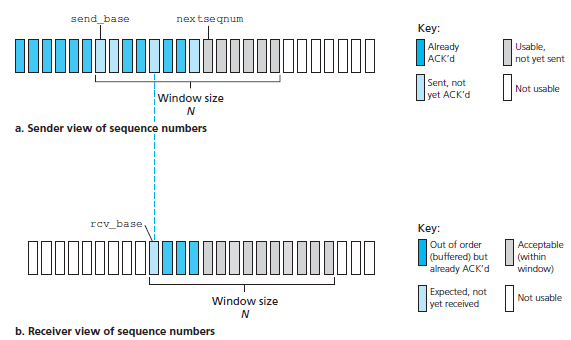
\includegraphics[width=0.62\linewidth]{cap09/sr_finestre.png}
    \caption{Selective Repeat: finestra del mittente (sopra) e del ricevente (sotto). Il ricevente accetta e conserva i pacchetti che cadono nella propria finestra, anche se fuori ordine.}
\end{figure}

\begin{figure}[H]
\centering
\begin{minipage}{0.48\linewidth}\centering
  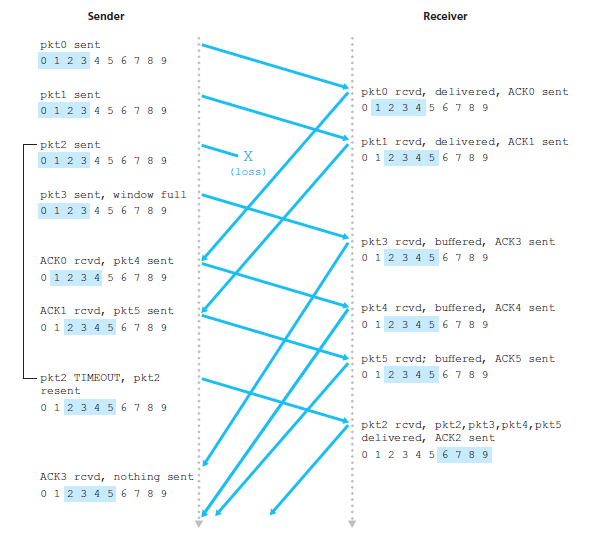
\includegraphics[width=0.95\linewidth]{cap09/sr_esempio.png}
\end{minipage}\hfill
\begin{minipage}{0.48\linewidth}
Stesso scenario di prima: finestra $N=4$, si perde il pacchetto 2.
\begin{itemize}
  \item Il ricevente conferma 0 e 1 e li consegna.
  \item Riceve 3, 4 e 5 fuori ordine: li \textbf{mette nel buffer} e li conferma singolarmente (ACK 3, ACK 4, ACK 5).
  \item Scade il timer del solo pacchetto 2, che viene ritrasmesso.
  \item Quando arriva pkt2, il ricevente consegna in blocco 2, 3, 4 e 5 all'applicazione.
\end{itemize}
Non si rispediscono pkt3, pkt4 e pkt5, evitando altre possibili perdite o errori.
\end{minipage}
\caption{Selective Repeat in azione.}
\end{figure}

\subsection{Il vincolo sui numeri di sequenza}

In SR la dimensione della finestra è legata al numero di sequenza, che è \textbf{finito} (il campo nell'header ha
un numero limitato di bit, e i numeri vengono riusati ciclicamente).

\begin{figure}[H]
\centering
\begin{minipage}{0.38\linewidth}\centering
  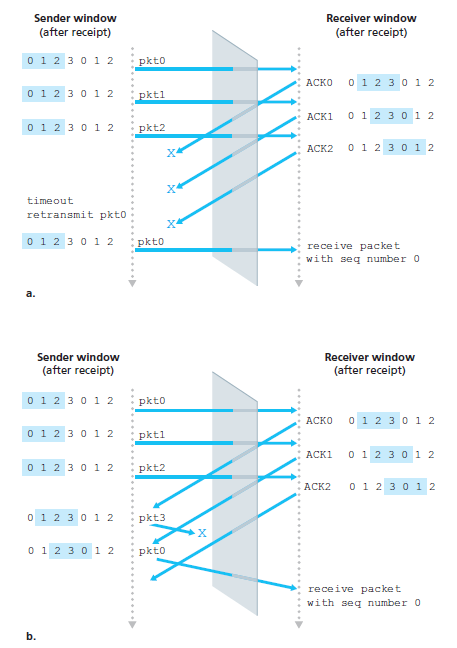
\includegraphics[width=0.9\linewidth]{cap09/sr_dilemma.png}
\end{minipage}\hfill
\begin{minipage}{0.58\linewidth}
Numeri di sequenza da 0 a 3 (quattro valori) e finestra di dimensione 3. I pacchetti 0, 1, 2 arrivano correttamente
e i loro ACK partono (ma non sono ancora arrivati). La finestra del ricevente avanza su $[3, 0, 1]$, anche se non è
certo che gli ACK siano arrivati.
\begin{itemize}
  \item \textbf{Caso (a)}: gli ACK dei primi tre pacchetti si perdono e il mittente, allo scadere dei timer,
        ritrasmette il pacchetto 0 (vecchio). Il ricevente lo accetta come \textbf{nuovo} pacchetto 0!
  \item \textbf{Caso (b)}: gli ACK arrivano, il mittente invia i nuovi 3 e 0, ma il 3 si perde. Il ricevente riceve
        uno 0 che stavolta è davvero nuovo.
\end{itemize}
Il ricevente \textbf{non può distinguere} i due casi: ai suoi occhi sono identici.
\end{minipage}
\caption{Il dilemma di Selective Repeat con finestra troppo grande.}
\end{figure}

\dfn{Vincolo della finestra}{
    Per evitare l'ambiguità, lo spazio dei numeri di sequenza deve essere \textbf{almeno il doppio} della
    dimensione della finestra:
    $$\text{numero di valori di sequenza} \geq 2N \quad\Longleftrightarrow\quad N \leq \frac{\text{numero di valori}}{2}$$
    Nell'esempio, con 4 valori la finestra può essere al massimo 2.
}

% ══════════════════════════════════════════════════════════════
\section{Riepilogo}
% ══════════════════════════════════════════════════════════════

\begin{table}[H]
\centering
\begin{tabular}{p{3cm}p{3.6cm}p{3.6cm}p{3.6cm}}
\toprule
 & \textbf{Stop-and-wait} & \textbf{Go-Back-N} & \textbf{Selective Repeat} \\
\midrule
Pacchetti in viaggio & 1 & fino a $N$ & fino a $N$ \\
Numeri di sequenza & 1 bit ($s=0/1$) & range più ampio & almeno $2N$ valori \\
ACK & per ogni pacchetto & cumulativi & individuali \\
Timer & uno & uno (pacchetto più vecchio) & uno per pacchetto \\
Fuori ordine al ricevente & --- & scartati & bufferizzati \\
Ritrasmissione & il pacchetto & tutti i non confermati & solo quelli persi \\
Complessità & minima & bassa & più alta \\
\bottomrule
\end{tabular}
\caption{I protocolli di trasferimento affidabile a confronto.}
\end{table}

\riepilogo{
\begin{itemize}
    \item Un canale affidabile garantisce bit non corrotti, niente perdite o duplicati, ordine corretto.
    \item Contro la corruzione: \textbf{checksum}, \textbf{ACK/NAK} e \textbf{numeri di sequenza} (ARQ).
    \item Contro le perdite: \textbf{timeout} e ritrasmissione; il timeout deve essere un po' più lungo dell'RTT.
    \item Lo stop-and-wait ha un \textbf{utilizzo} bassissimo: $U = \frac{L/R}{\text{RTT}+L/R}$.
    \item Il \textbf{pipelining} invia più pacchetti senza aspettare: \textbf{Go-Back-N} (ACK cumulativi, scarta i
          fuori ordine, ritrasmette tutto) e \textbf{Selective Repeat} (ACK individuali, bufferizza, ritrasmette
          solo i persi, sequenze $\geq 2N$).
\end{itemize}
}
     % Trasferimento affidabile
  \chapter{TCP: segmenti, numeri di sequenza e ritrasmissione}

% ══════════════════════════════════════════════════════════════
\section{TCP a confronto con UDP}
% ══════════════════════════════════════════════════════════════

Rispetto a UDP, TCP è:

\begin{itemize}
    \item \textbf{orientato alla connessione}: prima della trasmissione c'è una fase di \emph{handshake} che
          assicura che i due processi (mittente e ricevente) siano ``collegati'';
    \item \textbf{affidabile}: implementa rilevazione degli errori, ritrasmissioni, conferme, timer e numeri di sequenza;
    \item \textbf{attento al flusso e alla congestione}: regola la velocità di trasmissione in base alle capacità
          del ricevente (flusso) e allo stato della rete (congestione).
\end{itemize}

\dfn{Proprietà della connessione TCP}{
    \begin{itemize}
      \item \textbf{Full-duplex}: se l'host A è connesso con B, anche B è connesso con A, e i dati possono
            scorrere contemporaneamente nelle due direzioni.
      \item \textbf{Punto-punto}: un solo mittente e un solo ricevente. Non è possibile trasferire dati da un
            mittente a molti riceventi con una sola connessione (UDP, invece, permette il \emph{multicasting}).
      \item \textbf{Orientato al flusso di byte} (\emph{stream}): più segmenti TCP possono far parte di un unico
            flusso ordinato di dati, mentre i datagrammi UDP sono sostanzialmente indipendenti tra loro.
    \end{itemize}
}

% ══════════════════════════════════════════════════════════════
\section{I buffer TCP}
% ══════════════════════════════════════════════════════════════

In una connessione TCP l'invio e la ricezione si basano sui \textbf{buffer}. I buffer permettono di
disaccoppiare, almeno in parte, i tempi di trasmissione dai ritardi dell'applicazione, dai ritardi del
sistema operativo nel multiplexing e demultiplexing, e dalle oscillazioni delle prestazioni della rete.
Inoltre la velocità di trasmissione è limitata: i messaggi lunghi vengono spezzati in segmenti, che si
accumulano nei buffer prima di essere spediti (lato mittente) o riassemblati (lato ricevente).

\begin{figure}[H]
\centering
\begin{tikzpicture}[every node/.style={font=\footnotesize\sffamily}]
  \node[draw, circle, fill=lapp!60, minimum size=1cm] (pa) at (0,2) {A};
  \node[above=1pt of pa] {processo mittente};
  \node[field, fill=ltra!50, minimum width=0.6cm] (sk1) at (0,0.9) {};
  \node[left=2pt of sk1] {socket};
  \node[draw, fill=llink!50, minimum width=2.8cm, minimum height=0.8cm] (sb) at (0,-0.3) {};
  \foreach \x in {-1.1,-0.6,-0.1} \fill[netblue!60] (\x,-0.55) rectangle ++(0.4,0.5);
  \node[below=1pt of sb] {buffer di invio};
  \node[draw, circle, fill=lapp!60, minimum size=1cm] (pb) at (9,2) {B};
  \node[above=1pt of pb] {processo ricevente};
  \node[field, fill=ltra!50, minimum width=0.6cm] (sk2) at (9,0.9) {};
  \node[right=2pt of sk2] {socket};
  \node[draw, fill=llink!50, minimum width=2.8cm, minimum height=0.8cm] (rb) at (9,-0.3) {};
  \foreach \x in {8.0,8.5} \fill[netblue!60] (\x,-0.55) rectangle ++(0.4,0.5);
  \node[below=1pt of rb] {buffer di ricezione};
  \draw[-{Stealth}, thick] (pa) -- (sk1); \draw[-{Stealth}, thick] (sk1) -- (sb);
  \draw[-{Stealth}, thick] (rb) -- (sk2); \draw[-{Stealth}, thick] (sk2) -- (pb);
  \foreach \x in {3.4,4.5,5.6} { \fill[ltra] (\x,-0.5) rectangle ++(0.3,0.4); \fill[netblue!50] (\x+0.3,-0.5) rectangle ++(0.5,0.4); \draw (\x,-0.5) rectangle ++(0.8,0.4); }
  \draw[-{Stealth}, very thick, netblue] (sb.east) -- node[below=10pt] {segmenti} (rb.west);
\end{tikzpicture}
\caption{Ogni lato di una connessione TCP ha un buffer di invio e uno di ricezione.}
\end{figure}

\begin{itemize}
    \item \textbf{In invio}: i segmenti vengono creati a partire dai dati dell'applicazione e passati al livello di
          rete, dove ciascuno viene incapsulato in un datagramma IP.
    \item \textbf{In ricezione}: i dati vengono messi nel buffer di ricezione, e l'applicazione li preleva quando è pronta.
\end{itemize}

% ══════════════════════════════════════════════════════════════
\section{La Maximum Segment Size (MSS)}
% ══════════════════════════════════════════════════════════════

\dfn{MSS e MTU}{
    La quantità di dati applicativi in un segmento è limitata dalla \textbf{Maximum Segment Size} (MSS):
    $$\text{MSS} + 40 = \text{MTU}$$
    dove la \textbf{Maximum Transmission Unit} (MTU) è la lunghezza massima di un frame accettata dal livello
    di collegamento (in Ethernet \textbf{1500 byte}), e 40 è la somma tipica degli header TCP e IP (20 + 20 byte).
}

\begin{figure}[H]
\centering
\begin{tikzpicture}[every node/.style={font=\scriptsize\sffamily}]
  \node[field, fill=lnet, minimum width=2.2cm] (ip) at (0,0) {header IP: 20};
  \node[field, fill=ltra, minimum width=2.2cm, right=0pt of ip] (tcp) {header TCP: 20};
  \node[field, fill=lapp, minimum width=8cm, right=0pt of tcp] (d) {dati applicativi: al massimo MSS = 1460 byte};
  \draw[decorate, decoration={brace, amplitude=5pt}] ([yshift=2pt]ip.north west) -- ([yshift=2pt]d.north east) node[midway, above=6pt] {MTU di Ethernet = 1500 byte (payload del frame)};
\end{tikzpicture}
\caption{Con MTU di 1500 byte e header da 20 + 20 byte, la MSS tipica è di 1460 byte.}
\end{figure}

% ══════════════════════════════════════════════════════════════
\section{Il segmento TCP}
% ══════════════════════════════════════════════════════════════

\begin{figure}[H]
\centering
\begin{tikzpicture}[every node/.style={font=\scriptsize\sffamily}, x=0.45cm, y=0.62cm]
  \def\row#1#2#3#4{\node[field, fill=#4, minimum width=#2*0.45cm, minimum height=0.62cm, anchor=north west] at (#1,-#3) {};}
  % riga 1
  \node[field, fill=ltra, minimum width=7.2cm, minimum height=0.62cm, anchor=north west] at (0,0) {porta sorgente (16)};
  \node[field, fill=ltra, minimum width=7.2cm, minimum height=0.62cm, anchor=north west] at (16,0) {porta destinazione (16)};
  \node[field, fill=lapp!60, minimum width=14.4cm, minimum height=0.62cm, anchor=north west] at (0,-1) {numero di sequenza (32)};
  \node[field, fill=lapp!60, minimum width=14.4cm, minimum height=0.62cm, anchor=north west] at (0,-2) {numero di acknowledgment (32)};
  \node[field, fill=lnet!50, minimum width=1.8cm, minimum height=1.1cm, anchor=north west, align=center] at (0,-3) {lungh.\\header};
  \node[field, fill=lphy, minimum width=1.8cm, minimum height=1.1cm, anchor=north west, align=center] at (4,-3) {non\\usato};
  \foreach \f [count=\i from 0] in {CWR,ECE,URG,ACK,PSH,RST,SYN,FIN}
    \node[field, fill=netred!20, minimum width=0.45cm, minimum height=1.1cm, anchor=north west] at (8+\i,-3) {\rotatebox{90}{\f}};
  \node[field, fill=llink, minimum width=7.2cm, minimum height=1.1cm, anchor=north west] at (16,-3) {finestra di ricezione (16)};
  \node[field, fill=ltra!50, minimum width=7.2cm, minimum height=0.62cm, anchor=north west] at (0,-4.77) {checksum (16)};
  \node[field, fill=ltra!50, minimum width=7.2cm, minimum height=0.62cm, anchor=north west] at (16,-4.77) {puntatore ai dati urgenti (16)};
  \node[field, fill=lphy!60, minimum width=14.4cm, minimum height=0.62cm, anchor=north west] at (0,-5.77) {opzioni (lunghezza variabile)};
  \node[field, fill=cloudbg, minimum width=14.4cm, minimum height=1.3cm, anchor=north west] at (0,-6.77) {dati (al massimo MSS byte)};
  \draw[{Stealth}-{Stealth}] (0,0.5) -- node[above] {32 bit} (32,0.5);
  \draw[decorate, decoration={brace, amplitude=5pt}] (32.4,0) -- (32.4,-6.77) node[midway, right=6pt, align=left] {header:\\20 byte\\+ opzioni};
\end{tikzpicture}
\caption{La struttura del segmento TCP.}
\end{figure}

Il segmento TCP è fatto di un header e di un campo dati, che contiene al massimo MSS byte di dati
applicativi. I campi dell'header:

\begin{itemize}
    \item \textbf{porta sorgente} e \textbf{porta destinazione} (16 bit ciascuna): per multiplexing e demultiplexing;
    \item \textbf{numero di sequenza} (32 bit) e \textbf{numero di acknowledgment} (32 bit): per il trasferimento affidabile;
    \item \textbf{finestra di ricezione} (\emph{receive window}, 16 bit): il numero di byte che il ricevente è
          disposto ad accettare (serve al controllo di flusso);
    \item \textbf{lunghezza dell'header} (4 bit): il numero di parole da 32 bit dell'header. L'header TCP ha
          lunghezza variabile per via delle opzioni (tipicamente 20 byte senza opzioni);
    \item \textbf{opzioni} (lunghezza variabile): per processi facoltativi come la negoziazione della MSS o i timestamp;
    \item \textbf{flag}:
    \begin{itemize}
      \item \textbf{ACK}: il segmento contiene una conferma (il campo acknowledgment è valido);
      \item \textbf{RST}, \textbf{SYN}, \textbf{FIN}: apertura e chiusura della connessione;
      \item \textbf{CWR} e \textbf{ECE}: notifica esplicita della congestione (facoltativa);
      \item \textbf{PSH}: chiede al ricevente di passare subito i dati all'applicazione (raro);
      \item \textbf{URG}: il segmento contiene dati ``urgenti'' (raro);
    \end{itemize}
    \item \textbf{checksum} (16 bit): controllo di integrità, come in UDP;
    \item \textbf{puntatore ai dati urgenti} (16 bit): la posizione dell'ultimo byte dei dati urgenti (raro).
\end{itemize}

% ══════════════════════════════════════════════════════════════
\section{Numeri di sequenza e di acknowledgment}
% ══════════════════════════════════════════════════════════════

I numeri di sequenza non servono solo al trasferimento affidabile, ma anche a gestire la
\textbf{segmentazione}: un flusso di dati grande va spezzato in ``pezzi'' in base alla MSS, e ogni pezzo va in un
segmento. Numeri di sequenza e di acknowledgment sono strettamente legati.

TCP è un protocollo di trasporto generico: non sa nulla dei dati che trasporta. Per TCP i dati sono
solo un \textbf{flusso ordinato di byte}, e i numeri contano \textbf{byte}, non segmenti.

\dfn{Numero di sequenza e numero di acknowledgment}{
    \begin{itemize}
      \item Il \textbf{numero di sequenza} di un segmento è la posizione, nel flusso di byte, del \textbf{primo
            byte di dati} contenuto nel segmento.
      \item Il \textbf{numero di acknowledgment} è il numero di sequenza del \textbf{prossimo byte atteso} dal
            ricevente. Gli ACK di TCP sono \textbf{cumulativi}: ACK $n$ conferma tutti i byte fino a $n-1$.
    \end{itemize}
}

\begin{figure}[H]
\centering
\begin{tikzpicture}[every node/.style={font=\scriptsize\sffamily}]
  \draw[thick] (0,0) rectangle (14,0.7);
  \fill[lapp!70] (0,0) rectangle (2,0.7); \fill[ltra!70] (2,0) rectangle (4,0.7); \fill[lnet!70] (4,0) rectangle (6,0.7);
  \foreach \x in {2,4,6,8,10,12} \draw (\x,0) -- (\x,0.7);
  \node at (1,0.35) {segmento 1}; \node at (3,0.35) {segmento 2}; \node at (5,0.35) {segmento 3}; \node at (9,0.35) {\dots};
  \foreach \x/\n in {0/0, 2/1000, 4/2000, 6/3000} \node[below] at (\x,0) {\n};
  \node[below] at (13.9,0) {499\,999};
  \draw[{Stealth}-, thick, netred] (0,0.8) -- ++(0,0.6) node[above, text=netred] {seq = 0};
  \draw[{Stealth}-, thick, netred] (2,0.8) -- ++(0,0.6) node[above, text=netred] {seq = 1000};
  \draw[{Stealth}-, thick, netred] (4,0.8) -- ++(0,0.6) node[above, text=netred] {seq = 2000};
  \draw[decorate, decoration={brace, amplitude=5pt, mirror}] (0,-0.5) -- (2,-0.5) node[midway, below=6pt] {MSS = 1000 byte};
  \node[anchor=west] at (14.1,0.35) {file da 500\,000 byte};
\end{tikzpicture}
\caption{Un file di 500\,000 byte con MSS di 1000 byte: 500 segmenti, con numeri di sequenza 0, 1000, 2000, \dots}
\end{figure}

\begin{esempio}{Un file di 500 kB}
Un flusso di 500\,000 byte con MSS di 1000 byte diventa \textbf{500 segmenti}: il primo ha numero di
sequenza 0, il secondo 1000, il terzo 2000, e così via. Trascurando per semplicità lo scambio iniziale
(nella realtà il primo numero di sequenza è scelto a caso), dall'host A all'host B:
\begin{itemize}
    \item B riceve il primo segmento, con i byte da 0 a 999;
    \item B conferma con numero di acknowledgment \textbf{1000}: il prossimo byte che si aspetta;
    \item B riceve il secondo segmento, byte da 1000 a 1999, e conferma con ACK \textbf{2000}; e così via.
\end{itemize}
\end{esempio}

\warning{ACK $n$ non conferma il byte $n$}{
    L'errore più comune: ACK = 1000 \textbf{non} significa ``ho ricevuto il byte 1000'', ma ``ho ricevuto tutto
    fino al 999, mandami dal 1000 in poi''.
}

\subsection{Il caso full-duplex}

TCP è full-duplex: se A e B comunicano ci sono \textbf{due flussi} di dati da rendere affidabili, da A a B
e da B ad A. Si usano numeri di sequenza e di acknowledgment \textbf{contemporaneamente}:

\begin{itemize}
    \item i segmenti inviati da A hanno numeri di \textbf{sequenza} relativi al flusso A$\rightarrow$B e numeri di
          \textbf{acknowledgment} relativi al flusso B$\rightarrow$A;
    \item i segmenti inviati da B hanno numeri di sequenza relativi al flusso B$\rightarrow$A e numeri di
          acknowledgment relativi al flusso A$\rightarrow$B.
\end{itemize}

Un segmento può quindi portare \textbf{insieme dati e conferma} (si dice che l'ACK viaggia ``a cavalluccio'',
\emph{piggybacking}), con il flag ACK a 1.

\begin{esempio}{L'eco di un carattere (Telnet)}
\begin{center}
\begin{tikzpicture}[yscale=0.9, every node/.style={font=\scriptsize\sffamily}]
  \timeline{a}{0}{Host A}{5}
  \timeline{b}{7}{Host B}{5}
  \draw[msg, netgreen, very thick] (0,-0.5) -- node[above, sloped] {Seq=42, ACK=79, dati=`C'} (7,-1.5);
  \node[anchor=east, text width=2.6cm, align=right] at (-0.2,-0.5) {l'utente digita `C'};
  \draw[msg, netred, very thick] (7,-2.0) -- node[above, sloped] {Seq=79, ACK=43, dati=`C'} (0,-3.0);
  \node[anchor=west, text width=2.8cm, align=left] at (7.2,-2.0) {B conferma la `C' e la rimanda indietro (eco)};
  \draw[msg, netgreen, very thick] (0,-3.5) -- node[above, sloped] {Seq=43, ACK=80} (7,-4.5);
  \node[anchor=east, text width=2.6cm, align=right] at (-0.2,-3.5) {A conferma l'eco (ACK puro, senza dati)};
\end{tikzpicture}
\end{center}
Due messaggi da un solo byte: A invia la `C', che B rimanda indietro. In verde le informazioni sul flusso
A$\rightarrow$B, in rosso quelle sul flusso B$\rightarrow$A.
\begin{enumerate}
    \item \textbf{Da A a B}: il numero di sequenza è la posizione del byte trasmesso (42); l'ACK è il prossimo byte
          atteso sul flusso B$\rightarrow$A (79).
    \item \textbf{Da B ad A}: l'ACK è il prossimo byte atteso sul flusso A$\rightarrow$B, cioè $42 + 1$ byte $= 43$;
          il numero di sequenza è la posizione del byte che B trasmette (79), proprio quello che A aspettava.
    \item \textbf{Da A a B}: un ACK puro, con numero di sequenza 43 (come atteso da B) e ACK $79 + 1 = 80$.
\end{enumerate}
In ogni scambio vale: \textbf{ACK ricevuto = Seq inviato + byte inviati}, e \textbf{Seq inviato = ACK ricevuto}.
\end{esempio}

% ══════════════════════════════════════════════════════════════
\section{Il timeout di ritrasmissione}
% ══════════════════════════════════════════════════════════════

Il trasferimento affidabile di TCP usa ampiamente i timer. Nella trasmissione TCP con pipelining
l'approccio di base è ritrasmettere un segmento \textbf{solo se il suo ACK non arriva prima del timeout}.
La stima del timeout è quindi critica:

\begin{itemize}
    \item \textbf{troppo lungo}: la comunicazione rallenta, perché dopo una perdita si aspetta a lungo;
    \item \textbf{troppo breve}: si ritrasmettono segmenti non persi, producendo traffico inutile sulla rete.
\end{itemize}

\begin{figure}[H]
\centering
\begin{tikzpicture}[yscale=0.75, every node/.style={font=\scriptsize\sffamily}]
  \begin{scope}
    \node[font=\footnotesize\bfseries\sffamily] at (1.6,1.2) {(a) ACK perso};
    \timeline{a}{0}{A}{6}
    \timeline{b}{3.2}{B}{6}
    \draw[msg] (0,-0.3) -- node[above, sloped] {Seq=92, 8 byte} (3.2,-1.1);
    \draw[msglost] (3.2,-1.3) -- (1.7,-1.7); \node[text=netred] at (1.4,-1.35) {ACK=100};
    \draw[netorange, thick] (-0.25,-0.3) -- (-0.25,-2.9); \node[text=netorange, rotate=90] at (-0.5,-1.6) {timeout};
    \draw[msg] (0,-2.9) -- node[above, sloped] {Seq=92, 8 byte} (3.2,-3.7);
    \draw[msg, netgreen] (3.2,-3.9) -- node[above, sloped] {ACK=100} (0,-4.7);
  \end{scope}
  \begin{scope}[xshift=5.2cm]
    \node[font=\footnotesize\bfseries\sffamily] at (1.6,1.2) {(b) timeout prematuro};
    \timeline{a}{0}{A}{6}
    \timeline{b}{3.2}{B}{6}
    \draw[msg] (0,-0.3) -- node[above, sloped] {Seq=92, 8 byte} (3.2,-1.1);
    \draw[msg] (0,-0.6) -- node[below, sloped] {Seq=100, 20 byte} (3.2,-1.4);
    \draw[msg, netgreen] (3.2,-1.6) -- node[above, sloped, pos=0.3] {ACK=100} (0,-2.9);
    \draw[msg, netgreen] (3.2,-1.9) -- node[below, sloped, pos=0.7] {ACK=120} (0,-3.2);
    \draw[netorange, thick] (-0.25,-0.3) -- (-0.25,-2.5); \node[text=netorange, rotate=90] at (-0.5,-1.4) {timeout};
    \draw[msg, netred] (0,-2.5) -- node[above, sloped, pos=0.7] {Seq=92 (inutile)} (3.2,-3.5);
    \draw[msg, netgreen] (3.2,-3.7) -- node[above, sloped] {ACK=120} (0,-4.5);
  \end{scope}
  \begin{scope}[xshift=10.4cm]
    \node[font=\footnotesize\bfseries\sffamily] at (1.6,1.2) {(c) ACK cumulativo};
    \timeline{a}{0}{A}{6}
    \timeline{b}{3.2}{B}{6}
    \draw[msg] (0,-0.3) -- node[above, sloped] {Seq=92, 8 byte} (3.2,-1.1);
    \draw[msg] (0,-0.6) -- node[below, sloped] {Seq=100, 20 byte} (3.2,-1.4);
    \draw[msglost] (3.2,-1.6) -- (1.9,-2.0); \node[text=netred] at (1.5,-1.65) {ACK=100};
    \draw[msg, netgreen] (3.2,-2.2) -- node[above, sloped] {ACK=120} (0,-3.0);
    \node[text width=3cm, align=center] at (1.6,-4.1) {nessuna ritrasmissione: ACK=120 conferma anche i byte 92--99};
  \end{scope}
\end{tikzpicture}
\caption{Tre scenari di ritrasmissione TCP.}
\end{figure}

% ══════════════════════════════════════════════════════════════
\section{La stima dell'RTT}
% ══════════════════════════════════════════════════════════════

Per fissare il timeout serve una stima del \textbf{round-trip time}: il timeout (quanto aspettare l'ACK di un
segmento) deve essere maggiore dell'RTT, altrimenti si ritrasmette inutilmente.

TCP stima l'RTT misurando il tempo tra l'invio di un segmento e l'arrivo del suo ACK
(\textbf{SampleRTT}). Si campionano solo segmenti \textbf{confermati e non ritrasmessi}: per un segmento
ritrasmesso non si saprebbe a quale invio si riferisce l'ACK.

\dfn{EstimatedRTT}{
    Poiché i campioni oscillano (congestione, carico del ricevente, \dots), la stima è una \textbf{media mobile
    esponenziale pesata} (EWMA, \emph{Exponential Weighted Moving Average}):
    $$\text{EstimatedRTT} = (1-\alpha)\cdot\text{EstimatedRTT} + \alpha\cdot\text{SampleRTT}$$
    con $\alpha$ tipicamente $0{,}125 = 1/8$.
}

I campioni recenti pesano più di quelli vecchi, il cui peso decresce esponenzialmente: la stima segue
l'andamento reale ma senza farsi trascinare da ogni singolo picco.

\begin{figure}[H]
    \centering
    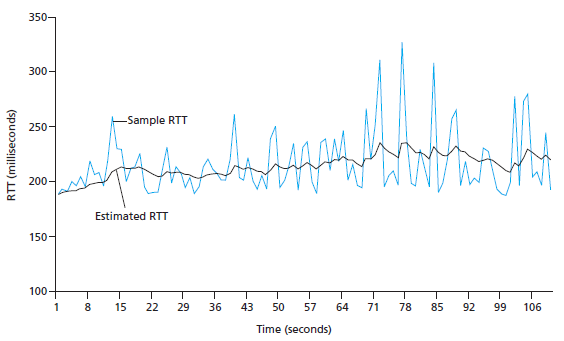
\includegraphics[width=0.62\linewidth]{cap10/rtt_campioni.png}
    \caption{Campioni di RTT (azzurro) e stima EWMA (nero) in una connessione reale tra Stati Uniti e Francia.}
\end{figure}

\dfn{DevRTT}{
    Si stima anche la \textbf{variabilità} dell'RTT, come media mobile della differenza tra campione e stima:
    $$\text{DevRTT} = (1-\beta)\cdot\text{DevRTT} + \beta\cdot|\,\text{SampleRTT} - \text{EstimatedRTT}\,|$$
    con $\beta$ tipicamente $0{,}25 = 1/4$.
}

\subsection{Il timeout}

\dfn{TimeoutInterval}{
    $$\text{TimeoutInterval} = \text{EstimatedRTT} + 4\cdot\text{DevRTT}$$
    La deviazione fornisce un \textbf{margine adattivo}: quando l'RTT oscilla molto il margine cresce, cioè si
    aspetta di più proprio quando si è meno sicuri dell'RTT. Il valore iniziale (a $t=0$) è di \textbf{1 secondo}.
}

\begin{esempio}{Aggiornare stima e timeout}
Siano $\text{EstimatedRTT} = 100$ ms, $\text{DevRTT} = 10$ ms, e arrivi un campione $\text{SampleRTT} = 140$ ms.
\begin{align*}
\text{EstimatedRTT} &= 0{,}875 \cdot 100 + 0{,}125 \cdot 140 = 87{,}5 + 17{,}5 = 105 \text{ ms}\\
\text{DevRTT} &= 0{,}75 \cdot 10 + 0{,}25 \cdot |140 - 105| = 7{,}5 + 8{,}75 = 16{,}25 \text{ ms}\\
\text{TimeoutInterval} &= 105 + 4 \cdot 16{,}25 = 170 \text{ ms}
\end{align*}
\end{esempio}

\info{Due dettagli pratici}{
    \begin{itemize}
      \item Nello standard (RFC 6298) \texttt{DevRTT} viene aggiornata \emph{prima} di \texttt{EstimatedRTT},
            usando il valore vecchio della stima; molti testi, come le trasparenze, le presentano nell'ordine
            inverso. Negli esercizi seguite l'ordine indicato dal testo.
      \item Quando scade un timeout, TCP ritrasmette e \textbf{raddoppia} il timeout, invece di ricalcolarlo: se c'è
            congestione, non ha senso ritrasmettere sempre più in fretta.
    \end{itemize}
}

% ══════════════════════════════════════════════════════════════
\section{Fast retransmit}
% ══════════════════════════════════════════════════════════════

La ritrasmissione dopo il timeout funziona, ma il timeout può essere relativamente lungo.

\dfn{Fast retransmit}{
    Con la \textbf{ritrasmissione veloce} il ricevente segnala al mittente che un segmento potrebbe essere
    perso inviando \textbf{ACK duplicati}.
    \begin{itemize}
      \item Se il ricevente riceve un segmento con numero di sequenza \textbf{più alto} di quello atteso, significa
            che probabilmente un segmento è andato perso.
      \item Il ricevente rimanda allora il vecchio ACK (\textbf{ACK duplicato}), con il numero del segmento atteso.
      \item Se il mittente riceve \textbf{3 ACK duplicati}, considera perso il segmento e lo ritrasmette subito,
            \textbf{molto prima} della scadenza del timeout.
    \end{itemize}
}

\begin{figure}[H]
\centering
\begin{minipage}{0.34\linewidth}\centering
  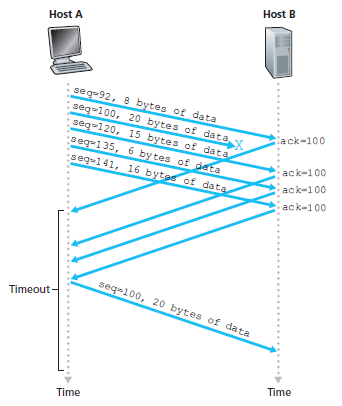
\includegraphics[width=0.9\linewidth]{cap10/fast_retransmit.png}
\end{minipage}\hfill
\begin{minipage}{0.62\linewidth}
\begin{itemize}
  \item Si perde il segmento con numero di sequenza 100.
  \item Ogni volta che B riceve un segmento fuori ordine, rimanda un ACK duplicato (ACK=100).
  \item Al terzo duplicato A considera perso il segmento 100 e lo rispedisce (fast retransmit), senza aspettare il timer.
  \item Quando B riceve finalmente il segmento mancante, invia l'ACK del prossimo segmento atteso secondo la propria
        politica (tipo Go-Back-N o Selective Repeat).
\end{itemize}
\end{minipage}
\caption{Ritrasmissione veloce dopo tre ACK duplicati.}
\end{figure}

\warning{Perché proprio tre duplicati?}{
    Perché non ritrasmettere al primo ACK duplicato? Perché un ACK ``sbagliato'' può arrivare anche per
    motivi diversi da una perdita. Per esempio, se due segmenti arrivano \textbf{scambiati di ordine}, il ricevente
    invia un ACK duplicato (per il primo segmento) prima di accorgersi dello scambio. Aspettare tre duplicati
    evita ritrasmissioni inutili dovute al semplice riordinamento.
}

% ══════════════════════════════════════════════════════════════
\section{Riepilogo}
% ══════════════════════════════════════════════════════════════

\riepilogo{
\begin{itemize}
    \item TCP è orientato alla connessione, affidabile, full-duplex, punto-punto e orientato al flusso di byte,
          con buffer di invio e ricezione.
    \item $\text{MSS} + 40 = \text{MTU}$ (in Ethernet MSS tipica 1460 byte).
    \item Header TCP: porte, \textbf{Seq}, \textbf{ACK}, lunghezza, flag (SYN, ACK, FIN, RST, \dots), finestra di
          ricezione, checksum, opzioni.
    \item Seq = numero del primo byte del segmento; ACK = prossimo byte atteso (cumulativo).
    \item $\text{EstimatedRTT} = 0{,}875\cdot\text{Est} + 0{,}125\cdot\text{Sample}$;
          $\text{DevRTT} = 0{,}75\cdot\text{Dev} + 0{,}25\cdot|\text{Sample}-\text{Est}|$;
          $\text{Timeout} = \text{Est} + 4\cdot\text{Dev}$.
    \item \textbf{Fast retransmit}: 3 ACK duplicati $\Rightarrow$ ritrasmissione immediata.
\end{itemize}
}
     % TCP: segmenti e ritrasmissione
  \chapter{TCP: la gestione della connessione}

% ══════════════════════════════════════════════════════════════
\section{Il problema}
% ══════════════════════════════════════════════════════════════

Poiché TCP è orientato alla connessione, i due host devono mettersi d'accordo sia quando la connessione
si \textbf{apre} sia quando si \textbf{chiude}. Ma i messaggi possono perdersi o danneggiarsi, e trovare un
accordo è tutt'altro che banale: se un messaggio si perde, un lato può ritenere la connessione aperta (o
chiusa) mentre l'altro no.

Per evitare, o meglio per \textbf{mitigare}, il problema TCP usa una procedura detta \textbf{three-way
handshake} (stretta di mano a tre vie): le richieste di apertura e di chiusura devono essere
\textbf{confermate} prima che la connessione sia considerata stabilita o rilasciata.

% ══════════════════════════════════════════════════════════════
\section{Il problema dei due eserciti}
% ══════════════════════════════════════════════════════════════

\begin{figure}[H]
\centering
\begin{tikzpicture}[every node/.style={font=\footnotesize\sffamily}]
  \fill[green!15] (-1,-1.2) -- (1.2,1.6) -- (3,0.4) -- (5,1.7) -- (7.4,-1.2) -- cycle;
  \fill[green!30] (-1,-1.2) -- (0.6,0.4) -- (2,-0.3) -- (3.2,-0.9) -- (4.8,-0.2) -- (6.2,0.5) -- (7.4,-1.2) -- cycle;
  \node[draw, fill=blue!40, rounded corners, minimum width=1.5cm] (b1) at (0.4,0.9) {blu \#1};
  \node[draw, fill=blue!40, rounded corners, minimum width=1.5cm] (b2) at (6,1.0) {blu \#2};
  \node[draw, fill=white, rounded corners, minimum width=2.6cm, minimum height=0.8cm] (w) at (3.2,-0.6) {esercito bianco};
  \draw[msg, dashed, netred, thick] (b1) to[bend right=15] node[below, sloped, text=netred] {messaggero} (b2);
  \node[text width=6.5cm, anchor=west] at (8,0.2) {Il bianco è più forte di ciascun esercito blu, ma più debole dei due insieme: i blu vincono solo se attaccano \textbf{nello stesso momento}. Per accordarsi possono mandare messaggeri attraverso la valle, dove possono essere catturati.};
\end{tikzpicture}
\caption{Il problema dei due eserciti: comunicare attraverso un canale inaffidabile.}
\end{figure}

Un esercito bianco è accampato in una valle; sulle due colline ai lati ci sono due eserciti blu. Il
bianco è più grande di ciascuno dei due eserciti blu, ma insieme i blu sono più numerosi: vincono
\textbf{solo se attaccano contemporaneamente}. Per sincronizzarsi devono mandare messaggeri attraverso la
valle, dove possono essere catturati (comunicazione \textbf{inaffidabile}). Esiste un protocollo che permetta
ai blu di vincere?

\begin{figure}[H]
\centering
\begin{tikzpicture}[yscale=0.8, every node/.style={font=\scriptsize\sffamily}]
  \begin{scope}
    \node[font=\footnotesize\bfseries\sffamily] at (1.9,1.1) {Due vie};
    \timeline{a}{0}{blu \#1}{3.4}
    \timeline{b}{3.8}{blu \#2}{3.4}
    \draw[msg] (0,-0.3) -- node[above, sloped] {``attacchiamo oggi, ok?''} (3.8,-1.1);
    \draw[msg, netgreen] (3.8,-1.4) -- node[above, sloped] {``d'accordo!''} (0,-2.2);
    \node[text=netred, anchor=west] at (3.9,-2.3) {sarà arrivato?};
  \end{scope}
  \begin{scope}[xshift=7.5cm]
    \node[font=\footnotesize\bfseries\sffamily] at (1.9,1.1) {Tre vie};
    \timeline{a}{0}{blu \#1}{3.4}
    \timeline{b}{3.8}{blu \#2}{3.4}
    \draw[msg] (0,-0.3) -- node[above, sloped] {``attacchiamo oggi, ok?''} (3.8,-1.1);
    \draw[msg, netgreen] (3.8,-1.4) -- node[above, sloped] {``d'accordo!''} (0,-2.2);
    \draw[msg] (0,-2.4) -- node[above, sloped] {``d'accordo!''} (3.8,-3.2);
    \node[text=netred, anchor=east] at (-0.1,-2.9) {e il mio, sarà arrivato?};
  \end{scope}
\end{tikzpicture}
\caption{Aggiungere conferme sposta solo il dubbio sull'ultimo messaggio.}
\end{figure}

\begin{itemize}
    \item Il comandante del blu \#1 manda: ``\emph{Propongo di attaccare oggi, va bene?}''. Il messaggio arriva, il
          blu \#2 è d'accordo e la sua risposta torna sana e salva. L'attacco ci sarà? Probabilmente no: il
          comandante \#2 \textbf{non sa} se la sua risposta è arrivata, e se non fosse arrivata il \#1 non attaccherebbe.
    \item Proviamo con tre vie: il \#1 conferma la risposta. Se nessun messaggio si perde, il \#2 riceve la conferma,
          ma ora è il \#1 a esitare: non sa se la sua conferma è arrivata.
    \item Con quattro vie non cambia nulla. Si può \textbf{dimostrare} che \textbf{non esiste alcun protocollo} che
          risolva il problema con certezza.
\end{itemize}

\info{Imperfetto ma adeguato}{
    Il three-way handshake \textbf{non è perfetto}, ma nella pratica è di solito \textbf{più che adeguato}: le
    situazioni residue vengono gestite con timer e ritrasmissioni.
}

% ══════════════════════════════════════════════════════════════
\section{L'apertura della connessione}
% ══════════════════════════════════════════════════════════════

\begin{enumerate}
    \item Il client invia una richiesta di connessione: un segmento \textbf{SYN}.
    \item Il server risponde con una conferma speciale: un segmento \textbf{SYN-ACK} (o SYNACK).
    \item Il client invia la conferma finale: un segmento \textbf{ACK}.
\end{enumerate}

\subsection{I dettagli}

\begin{figure}[H]
\centering
\begin{tikzpicture}[yscale=0.9, every node/.style={font=\footnotesize\sffamily}]
  \timeline{c}{0}{Client}{5.2}
  \timeline{s}{8}{Server}{5.2}
  \node[anchor=east, text=black!60] at (-0.2,0) {\texttt{connect()}};
  \node[anchor=west, text=black!60] at (8.2,0) {\texttt{listen()}, \texttt{accept()}};
  \draw[msg, very thick, netblue] (0,-0.5) -- node[above, sloped, align=center] {SYN = 1, Seq = client\_isn\\(nessun dato)} (8,-1.7);
  \node[anchor=west, text width=3.4cm, align=left] at (8.2,-1.9) {alloca buffer e variabili};
  \draw[msg, very thick, netgreen] (8,-2.2) -- node[above, sloped, align=center] {SYN = 1, ACK = 1, Seq = server\_isn\\Ack = client\_isn + 1} (0,-3.4);
  \node[anchor=east, text width=3cm, align=right] at (-0.2,-3.6) {alloca buffer e variabili};
  \draw[msg, very thick, netblue] (0,-3.9) -- node[above, sloped, align=center] {SYN = 0, ACK = 1, Seq = client\_isn + 1\\Ack = server\_isn + 1 (può contenere dati)} (8,-5.1);
  \node[anchor=west, text=netgreen!60!black, font=\footnotesize\bfseries\sffamily] at (8.2,-5.1) {connessione stabilita};
\end{tikzpicture}
\caption{Il three-way handshake nel dettaglio.}
\end{figure}

\begin{enumerate}
    \item Il client invia un segmento \textbf{SYN} che ha:
    \begin{itemize}
      \item \textbf{nessun dato} applicativo;
      \item il bit \textbf{SYN a 1};
      \item come numero di sequenza un \textbf{numero iniziale casuale} (\texttt{client\_isn}, \emph{initial sequence number}).
    \end{itemize}
    \item Quando il SYN arriva (si spera), il server \textbf{alloca buffer e variabili} TCP e risponde con un segmento
          \textbf{SYNACK} che ha:
    \begin{itemize}
      \item nessun dato applicativo;
      \item i bit \textbf{SYN e ACK a 1};
      \item numero di acknowledgment \texttt{client\_isn + 1};
      \item come numero di sequenza un proprio numero iniziale casuale (\texttt{server\_isn}).
    \end{itemize}
    \item Quando il SYNACK arriva (si spera), anche il client alloca buffer e variabili e invia un segmento
          \textbf{ACK} finale che ha:
    \begin{itemize}
      \item eventualmente \textbf{dati} applicativi (per esempio la richiesta HTTP);
      \item il bit \textbf{SYN a 0} (la connessione ora è stabilita) e il bit \textbf{ACK a 1};
      \item numero di acknowledgment \texttt{server\_isn + 1}.
    \end{itemize}
\end{enumerate}

\warning{Perché il SYN ``consuma'' un numero di sequenza}{
    Il SYN non porta dati, eppure l'ACK di risposta vale \texttt{client\_isn + 1}: per convenzione SYN (e FIN)
    contano come un byte, così possono essere confermati come qualsiasi altro dato. I numeri iniziali sono
    \textbf{casuali} per evitare che segmenti di una vecchia connessione, ancora in giro per la rete, vengano
    scambiati per segmenti della nuova.
}

\warning{Un momento delicato}{
    L'apertura della connessione è delicata e può aggiungere ritardi significativi. Di solito c'è un
    \textbf{timeout} (30--60 secondi) per completare l'handshake, dopo il quale la procedura viene abbandonata. Qui
    avvengono anche alcuni attacchi: nel \textbf{SYN flood} l'attaccante invia moltissimi SYN senza mai completare
    l'handshake, costringendo il server ad allocare risorse per migliaia di connessioni ``mezze aperte''.
}

\subsection{Diagramma degli stati (apertura)}

\begin{figure}[H]
\centering
\begin{tikzpicture}[every node/.style={font=\scriptsize\sffamily}, st/.style={draw, rounded corners=6pt, fill=cloudbg, thick, minimum width=2.4cm, minimum height=0.75cm, font=\footnotesize\bfseries\sffamily}]
  \node[st] (closed) at (0,0) {CLOSED};
  \node[st] (listen) at (-4,-2) {LISTEN};
  \node[st] (synsent) at (4,-2) {SYN SENT};
  \node[st] (synrcvd) at (-4,-4.3) {SYN RECEIVED};
  \node[st, fill=netgreen!20] (est) at (0,-6.3) {ESTABLISHED};
  \draw[-{Stealth}, thick] (closed) -- node[above, sloped, align=center] {apertura passiva\\\texttt{listen()}} (listen);
  \draw[-{Stealth}, thick] (closed) -- node[above, sloped, align=center] {apertura attiva: \texttt{connect()}\\invia SYN} (synsent);
  \draw[-{Stealth}, thick] (listen) -- node[left, align=right] {ricevuto SYN\\invia SYN+ACK} (synrcvd);
  \draw[-{Stealth}, thick] (synsent) -- node[right, align=left] {ricevuto SYN+ACK\\invia ACK} (est);
  \draw[-{Stealth}, thick] (synrcvd) -- node[below left, align=right] {ricevuto ACK} (est);
  \node[text=netblue, font=\footnotesize\bfseries\sffamily] at (-4,-0.9) {server};
  \node[text=netred, font=\footnotesize\bfseries\sffamily] at (4,-0.9) {client};
\end{tikzpicture}
\caption{Diagramma degli stati semplificato per l'apertura della connessione.}
\end{figure}

% ══════════════════════════════════════════════════════════════
\section{La chiusura della connessione}
% ══════════════════════════════════════════════════════════════

La chiusura (\emph{teardown}) può essere avviata da \textbf{uno qualsiasi} dei due host. Supponiamo che a
chiudere sia il client:

\begin{figure}[H]
\centering
\begin{tikzpicture}[yscale=0.85, every node/.style={font=\footnotesize\sffamily}]
  \timeline{c}{0}{Client}{5.8}
  \timeline{s}{7}{Server}{5.8}
  \node[anchor=east, text=black!60] at (-0.2,-0.4) {\texttt{close()}};
  \draw[msg, very thick, netred] (0,-0.5) -- node[above, sloped] {FIN = 1} (7,-1.4);
  \draw[msg, very thick, netgreen] (7,-1.7) -- node[above, sloped] {ACK = 1} (0,-2.6);
  \node[anchor=west, text=black!60] at (7.2,-2.9) {\texttt{close()}};
  \draw[msg, very thick, netred] (7,-3.0) -- node[above, sloped] {FIN = 1} (0,-3.9);
  \draw[msg, very thick, netgreen] (0,-4.2) -- node[above, sloped] {ACK = 1} (7,-5.1);
  \node[anchor=west, text=netgreen!60!black, font=\footnotesize\bfseries\sffamily] at (7.2,-5.1) {chiusa};
  \draw[netorange, very thick] (-0.3,-4.2) -- (-0.3,-5.8);
  \node[anchor=east, text=netorange, text width=2.6cm, align=right] at (-0.4,-5.0) {attesa (TIME WAIT), poi chiusa};
\end{tikzpicture}
\caption{La chiusura della connessione: ACK e FIN del server possono viaggiare nello stesso segmento o in due segmenti separati.}
\end{figure}

\begin{enumerate}
    \item Il client invia un segmento speciale di chiusura: un segmento \textbf{FIN}, con il bit FIN a 1.
    \item Quando lo riceve, il server invia una conferma e, quando anche lui ha finito, un proprio segmento di
          chiusura, con ACK a 1 e FIN a 1. ACK e FIN possono viaggiare nello stesso segmento o in due separati:
          nel mezzo il server può ancora inviare dati (la connessione è chiusa solo in una direzione).
    \item Infine il client conferma il FIN del server.
\end{enumerate}

\subsection{Diagramma degli stati (chiusura)}

\begin{figure}[H]
\centering
\begin{tikzpicture}[every node/.style={font=\scriptsize\sffamily}, st/.style={draw, rounded corners=6pt, fill=cloudbg, thick, minimum width=2.3cm, minimum height=0.7cm, font=\footnotesize\bfseries\sffamily}]
  \node[st, fill=netgreen!20] (est) at (0,0) {ESTABLISHED};
  \node[st] (fw1) at (-4,-1.8) {FIN WAIT 1};
  \node[st] (fw2) at (-4,-3.8) {FIN WAIT 2};
  \node[st] (closing) at (-0.6,-3.8) {CLOSING};
  \node[st] (tw) at (-4,-5.8) {TIME WAIT};
  \node[st] (cw) at (4,-1.8) {CLOSE WAIT};
  \node[st] (la) at (4,-3.8) {LAST ACK};
  \node[st, fill=lphy] (closed) at (0,-7.4) {CLOSED};
  \draw[-{Stealth}, thick] (est) -- node[above, sloped, align=center] {\texttt{close()}\\invia FIN} (fw1);
  \draw[-{Stealth}, thick] (fw1) -- node[left, align=right] {ricevuto ACK} (fw2);
  \draw[-{Stealth}, thick] (fw1) -- node[above, sloped, align=center] {ricevuto FIN\\invia ACK} (closing);
  \draw[-{Stealth}, thick] (fw2) -- node[left, align=right] {ricevuto FIN\\invia ACK} (tw);
  \draw[-{Stealth}, thick] (closing) -- node[right, align=left] {ricevuto ACK} (tw);
  \draw[-{Stealth}, thick] (tw) -- node[below left, align=right] {scade il timeout} (closed);
  \draw[-{Stealth}, thick] (est) -- node[above, sloped, align=center] {ricevuto FIN\\invia ACK} (cw);
  \draw[-{Stealth}, thick] (cw) -- node[right, align=left] {\texttt{close()}\\invia FIN} (la);
  \draw[-{Stealth}, thick] (la) -- node[below right, align=left] {ricevuto ACK} (closed);
  \node[text=netred, font=\footnotesize\bfseries\sffamily] at (-4,-0.8) {chi chiude per primo};
  \node[text=netblue, font=\footnotesize\bfseries\sffamily] at (4,-0.8) {chi chiude per secondo};
\end{tikzpicture}
\caption{Diagramma degli stati semplificato per il rilascio della connessione. CLOSING corrisponde al caso raro in cui i due lati chiudono contemporaneamente.}
\end{figure}

\info{A cosa serve TIME WAIT}{
    Chi chiude per primo non passa subito a CLOSED: resta in \textbf{TIME WAIT} per un tempo pari a due volte la
    vita massima di un segmento in rete (da 30 secondi a qualche minuto). Così, se l'ultimo ACK si perde e il pari
    ritrasmette il suo FIN, c'è ancora qualcuno che può riconfermarlo; e i segmenti vecchi della connessione
    hanno il tempo di sparire prima che la stessa coppia di porte venga riusata. È il motivo per cui, nel capitolo
    sui socket, un server chiuso male poteva lasciare la porta occupata per alcuni minuti.
}

% ══════════════════════════════════════════════════════════════
\section{Come TCP si salva dalla perdita di pacchetti}
% ══════════════════════════════════════════════════════════════

Poiché il three-way handshake non è perfetto, TCP si affida ai \textbf{timer} per chiudere comunque le
connessioni o per ripetere le richieste. Alcuni esempi durante il rilascio:

\begin{figure}[H]
\centering
\begin{tikzpicture}[yscale=0.72, every node/.style={font=\scriptsize\sffamily}]
  \begin{scope}
    \node[font=\footnotesize\bfseries\sffamily] at (1.6,1.1) {(a) si perde l'ACK finale};
    \timeline{c}{0}{Client}{7}
    \timeline{s}{3.2}{Server}{7}
    \draw[msg] (0,-0.3) -- node[above, sloped] {FIN} (3.2,-1.0);
    \draw[msg, netgreen] (3.2,-1.2) -- node[above, sloped] {ACK + FIN} (0,-1.9);
    \draw[msglost] (0,-2.1) -- (1.7,-2.5); \node[text=netred] at (2.1,-2.2) {ACK perso};
    \draw[netorange, thick] (3.45,-1.2) -- (3.45,-3.6); \node[text=netorange, rotate=90] at (3.7,-2.4) {timeout};
    \draw[msg] (3.2,-3.6) -- node[above, sloped] {FIN (di nuovo)} (0,-4.3);
    \draw[msg, netgreen] (0,-4.5) -- node[above, sloped] {ACK} (3.2,-5.2);
    \node at (1.6,-6.2) {chiusa su entrambi i lati};
  \end{scope}
  \begin{scope}[xshift=5.6cm]
    \node[font=\footnotesize\bfseries\sffamily] at (1.6,1.1) {(b) si perde il FIN del server};
    \timeline{c}{0}{Client}{7}
    \timeline{s}{3.2}{Server}{7}
    \draw[msg] (0,-0.3) -- node[above, sloped] {FIN} (3.2,-1.0);
    \draw[msglost] (3.2,-1.2) -- (1.5,-1.6); \node[text=netred] at (1.1,-1.3) {perso};
    \draw[netorange, thick] (-0.25,-0.3) -- (-0.25,-2.6); \node[text=netorange, rotate=90] at (-0.5,-1.45) {timeout};
    \draw[msg] (0,-2.6) -- node[above, sloped] {FIN (rinviato)} (3.2,-3.3);
    \draw[msg, netgreen] (3.2,-3.5) -- node[above, sloped] {ACK + FIN} (0,-4.2);
    \draw[msg, netgreen] (0,-4.4) -- node[above, sloped] {ACK} (3.2,-5.1);
    \node at (1.6,-6.2) {chiusa su entrambi i lati};
  \end{scope}
  \begin{scope}[xshift=11.2cm]
    \node[font=\footnotesize\bfseries\sffamily] at (1.6,1.1) {(c) perdite ripetute};
    \timeline{c}{0}{Client}{7}
    \timeline{s}{3.2}{Server}{7}
    \draw[msg] (0,-0.3) -- node[above, sloped] {FIN} (3.2,-1.0);
    \draw[msglost] (3.2,-1.2) -- (1.5,-1.6);
    \draw[msg] (0,-2.4) -- node[above, sloped] {FIN} (3.2,-3.1);
    \draw[msglost] (3.2,-3.3) -- (1.5,-3.7);
    \node[text width=2.8cm, align=center] at (1.6,-5.0) {dopo $N$ timeout ciascun lato chiude comunque};
    \node[text=netred] at (0,-6.5) {chiusa}; \node[text=netred] at (3.2,-6.5) {chiusa};
  \end{scope}
\end{tikzpicture}
\caption{Timer e ritrasmissioni permettono di chiudere la connessione anche quando si perdono segmenti; dopo un certo numero di tentativi falliti la connessione viene chiusa d'ufficio.}
\end{figure}

\warning{RST: il rifiuto}{
    Se arriva un SYN per una porta su cui nessun processo è in ascolto, l'host risponde con un segmento con il bit
    \textbf{RST} a 1 (\emph{reset}): ``qui non c'è nessuno''. Lo stesso bit serve a interrompere bruscamente una
    connessione in uno stato anomalo. Nel caso di UDP, invece, a una porta chiusa si risponde con un messaggio ICMP
    ``port unreachable'' (lo vedremo con traceroute).
}

% ══════════════════════════════════════════════════════════════
\section{Riepilogo}
% ══════════════════════════════════════════════════════════════

\riepilogo{
\begin{itemize}
    \item Accordarsi su un canale inaffidabile con certezza è impossibile (\textbf{problema dei due eserciti}): il
          three-way handshake è imperfetto ma adeguato.
    \item \textbf{Apertura}: SYN (Seq = client\_isn), SYNACK (Seq = server\_isn, Ack = client\_isn+1), ACK (Ack =
          server\_isn+1, può contenere dati). Numeri iniziali casuali.
    \item Stati di apertura: CLOSED, LISTEN / SYN SENT, SYN RECEIVED, ESTABLISHED.
    \item \textbf{Chiusura}: FIN, ACK, FIN, ACK (ACK e FIN possono essere uniti); stati FIN WAIT 1/2, CLOSE WAIT,
          LAST ACK, CLOSING, TIME WAIT, CLOSED.
    \item I \textbf{timer} risolvono le perdite residue; RST rifiuta o interrompe le connessioni.
\end{itemize}
}
     % TCP: connessione
  \chapter{Controllo di flusso e controllo di congestione}

% ══════════════════════════════════════════════════════════════
\section{Il problema comune: i buffer che traboccano}
% ══════════════════════════════════════════════════════════════

Oltre all'affidabilità, TCP offre rispetto a UDP il \textbf{controllo di flusso} e il \textbf{controllo di
congestione}. Entrambi nascono dallo stesso fatto: la perdita di pacchetti è spesso dovuta al
\textbf{traboccare di un buffer}.

\begin{itemize}
    \item Il \textbf{buffer di ricezione} del destinatario trabocca se l'applicazione non legge i dati abbastanza
          in fretta $\Rightarrow$ problema di \textbf{flusso}.
    \item I \textbf{buffer dei dispositivi di rete} (i router) traboccano se i nodi sono congestionati
          $\Rightarrow$ problema di \textbf{congestione}.
\end{itemize}

\begin{figure}[H]
\centering
\begin{tikzpicture}[every node/.style={font=\footnotesize\sffamily}]
  \draw[thick] (0,0) -- (0,1.4) -- (1.4,1.4) -- (1.4,0); \fill[netblue!50] (0.02,0.02) rectangle (1.38,1.1);
  \node at (0.7,-0.3) {mittente};
  \draw[thick, netblue!70, line width=4pt] (1.4,0.4) -- (4.2,0.4);
  \draw[thick] (4.2,0.6) -- (4.2,1.8) -- (5.6,1.8) -- (5.6,0.6) -- cycle; \fill[netblue!50] (4.22,0.62) rectangle (5.58,1.8);
  \foreach \x in {4.4,4.9,5.3} \fill[netblue!60] (\x,1.85) circle (2pt);
  \node[text=netred] at (4.9,2.3) {trabocca!};
  \node at (4.9,0.3) {router (congestione)};
  \draw[thick, netblue!70, line width=4pt] (5.6,0.9) -- (8.2,0.9);
  \draw[thick] (8.2,0.5) -- (8.2,1.9) -- (9.6,1.9) -- (9.6,0.5) -- cycle; \fill[netblue!50] (8.22,0.52) rectangle (9.58,1.7);
  \draw[thick, netblue!70, line width=1.2pt] (9.6,0.7) -- (10.6,0.7);
  \node[align=center] at (8.9,0.1) {buffer di ricezione\\(flusso)};
  \node[align=center] at (11.2,0.7) {applicazione\\lenta};
\end{tikzpicture}
\caption{L'analogia dell'acqua: i buffer sono secchi intermedi che traboccano se entra più acqua di quanta ne esca.}
\end{figure}

Se i pacchetti si perdono, gli host devono affidarsi a ritrasmissioni e timeout, che peggiorano
drasticamente le prestazioni della rete. Meglio evitare di arrivarci.

% ══════════════════════════════════════════════════════════════
\section{Il controllo di flusso}
% ══════════════════════════════════════════════════════════════

Quando TCP riceve byte corretti e in sequenza, li mette nel \textbf{buffer di ricezione}. L'applicazione li
legge da lì, ma non necessariamente nell'istante in cui arrivano (può essere occupata). Se l'applicazione è
lenta a leggere, il mittente può facilmente far traboccare il buffer inviando troppi dati troppo in fretta.

\dfn{Controllo di flusso}{
    Il \textbf{controllo di flusso} di TCP è un servizio di \textbf{adeguamento della velocità}
    (\emph{speed-matching}): cerca di adeguare (ridurre) il ritmo di invio del mittente al ritmo con cui
    l'\textbf{applicazione ricevente} legge i dati. Si basa sulla \textbf{finestra di ricezione}
    (\emph{receive window}, rwnd), il campo dell'header TCP con cui il ricevente comunica al mittente quanto
    spazio libero gli resta nel buffer.
}

\begin{figure}[H]
    \centering
    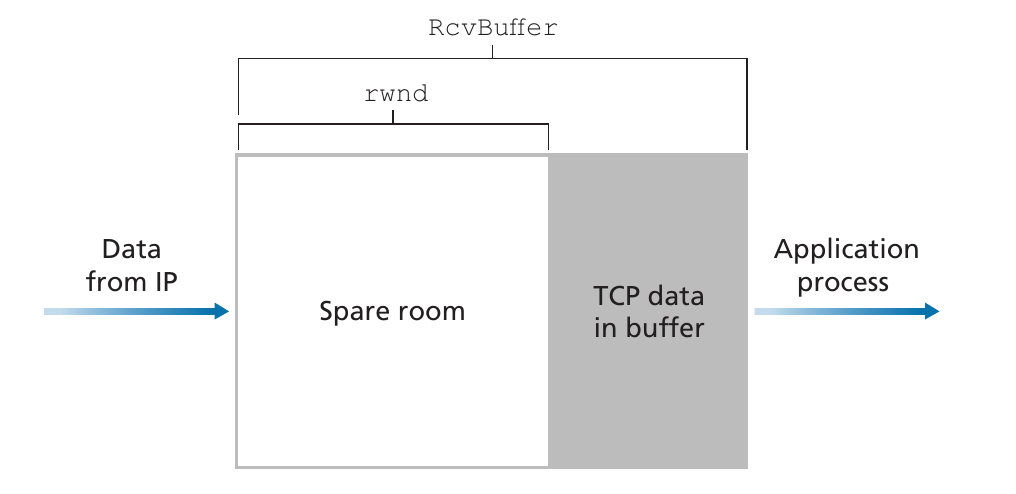
\includegraphics[width=0.55\linewidth]{cap12/rwnd_buffer.png}
    \caption{Il buffer di ricezione: la parte grigia contiene dati non ancora letti dall'applicazione, la parte bianca (rwnd) è lo spazio libero.}
\end{figure}

\subsection{Le formule}

Supponiamo per semplicità che il ricevente scarti i segmenti fuori ordine, così che tutti i dati nel buffer
siano in ordine. Sul \textbf{ricevente} (host B) si definiscono:

\begin{itemize}
    \item \texttt{RcvBuffer}: la dimensione del buffer di ricezione (in byte);
    \item \texttt{LastByteRead}: l'ultimo byte del flusso letto dall'applicazione;
    \item \texttt{LastByteRcvd}: l'ultimo byte del flusso arrivato e messo nel buffer.
\end{itemize}

\dfn{Finestra di ricezione}{
    $$\text{rwnd} = \text{RcvBuffer} - (\text{LastByteRcvd} - \text{LastByteRead})$$
    cioè lo spazio totale meno i byte ricevuti ma non ancora letti.
}

Sul \textbf{mittente} (host A) si tengono \texttt{LastByteSent} (l'ultimo byte inviato) e \texttt{LastByteAcked}
(l'ultimo byte confermato dal ricevente). Conoscendo la finestra comunicata da B, il mittente garantisce in
ogni istante:

$$\text{LastByteSent} - \text{LastByteAcked} \leq \text{rwnd}$$

cioè i byte ``in volo'' (inviati ma non confermati) non superano mai lo spazio libero del ricevente.

\begin{figure}[H]
\centering
\begin{tikzpicture}[every node/.style={font=\scriptsize\sffamily}]
  \foreach \i in {0,...,15} {
    \pgfmathsetmacro{\c}{\i<5 ? "lnet" : (\i<9 ? "llink" : (\i<12 ? "white" : "lphy"))}
    \node[draw, fill=\c, minimum width=0.7cm, minimum height=0.6cm] at (\i*0.7,0) {};
  }
  \draw[decorate, decoration={brace, amplitude=5pt}] (-0.35,0.4) -- (3.15,0.4) node[midway, above=6pt] {inviati e confermati};
  \draw[decorate, decoration={brace, amplitude=5pt}] (3.15,0.4) -- (5.95,0.4) node[midway, above=6pt, align=center] {inviati, non confermati};
  \draw[decorate, decoration={brace, amplitude=5pt}] (5.95,0.4) -- (8.05,0.4) node[midway, above=6pt, align=center] {inviabili};
  \draw[decorate, decoration={brace, amplitude=5pt}] (8.05,0.4) -- (11.2,0.4) node[midway, above=6pt] {non ancora inviabili};
  \draw[decorate, decoration={brace, amplitude=5pt, mirror}] (3.15,-0.4) -- (8.05,-0.4) node[midway, below=6pt, text=netred] {rwnd};
  \node[below=16pt] at (3.15,-0.2) {LastByteAcked};
  \node[below=16pt] at (5.95,-0.9) {LastByteSent};
  \draw[-{Stealth}] (5.95,-1.15) -- (5.95,-0.35);
\end{tikzpicture}
\caption{Lato mittente: il flusso di byte e la finestra consentita dal ricevente.}
\end{figure}

\begin{esempio}{Calcolare la finestra}
B ha un buffer da 4000 byte. Ha ricevuto fino al byte 3000 (\texttt{LastByteRcvd} = 3000) e l'applicazione ha letto
fino al byte 1000 (\texttt{LastByteRead} = 1000). Allora:
$$\text{rwnd} = 4000 - (3000 - 1000) = 2000 \text{ byte}$$
B scrive 2000 nel campo finestra dei segmenti che invia ad A. Se A ha già inviato fino al byte 3500 e ha ricevuto
conferma fino al 3000, ha 500 byte in volo e può inviarne ancora al massimo $2000 - 500 = 1500$.
\end{esempio}

\warning{Finestra a zero}{
    Se il buffer di B si riempie, B comunica $\text{rwnd} = 0$ e A si ferma. Ma se B non ha dati da inviare, non
    manderà più segmenti, e A non saprebbe mai che si è liberato spazio! Per evitare il blocco, quando la finestra è
    zero il mittente continua a inviare periodicamente segmenti di \textbf{un byte} (\emph{zero window probe}): le
    risposte di B contengono il valore aggiornato della finestra.
}

% ══════════════════════════════════════════════════════════════
\section{Il problema della congestione}
% ══════════════════════════════════════════════════════════════

Il problema della congestione è simile a quello del flusso, ma riguarda l'\textbf{infrastruttura di rete}
invece del ricevente.

\subsection{Scenario 1: buffer infinito}

\begin{figure}[H]
    \centering
    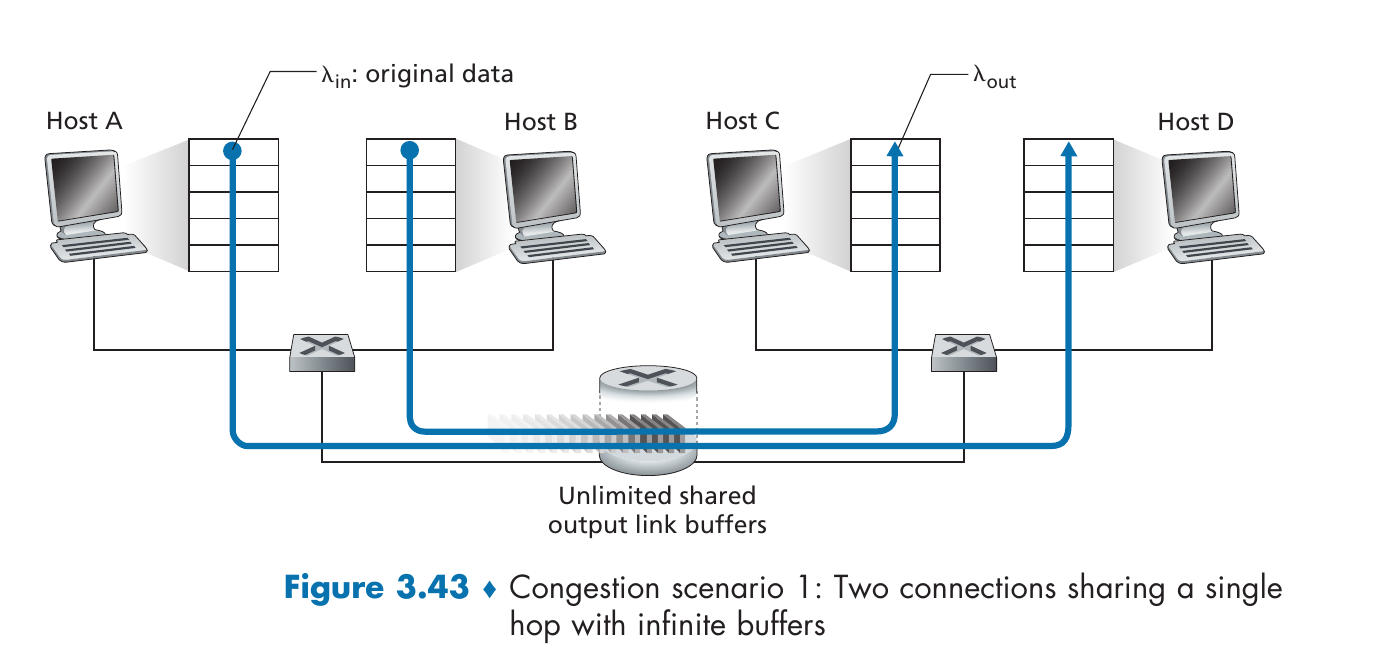
\includegraphics[width=0.55\linewidth]{cap12/scenario1.png}
    \caption{Due connessioni condividono un solo router con buffer infinito e un collegamento in uscita di capacità $R$.}
\end{figure}

Due host (A e B) hanno ciascuno una connessione che attraversa lo stesso router e lo stesso collegamento
in uscita di capacità $R$. Il router ha dei buffer che conservano i pacchetti quando la velocità di arrivo
supera la capacità del collegamento. Entrambe le applicazioni inviano dati alla stessa velocità media di
$\lambda_{in}$ byte/s.

\begin{figure}[H]
    \centering
    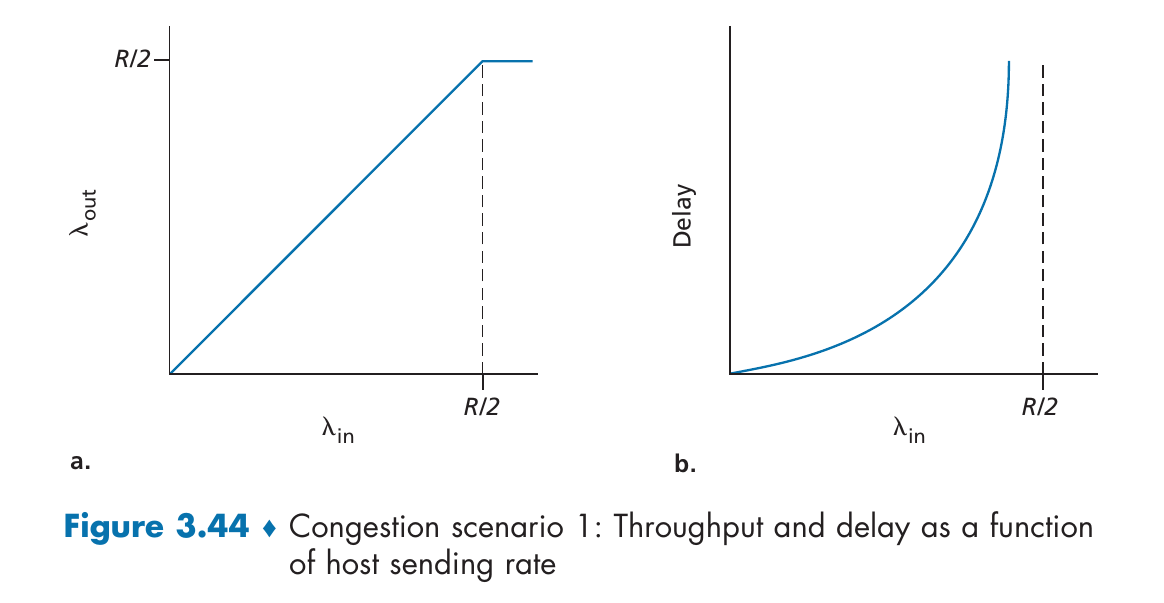
\includegraphics[width=0.6\linewidth]{cap12/scenario1_grafici.png}
    \caption{(a) Throughput per connessione in funzione della velocità di invio: non supera $R/2$. (b) Ritardo: cresce senza limite avvicinandosi a $R/2$.}
\end{figure}

\begin{itemize}
    \item Se $\lambda_{in} < R/2$, tutto ciò che il mittente invia arriva al ricevente con un ritardo finito.
    \item Se $\lambda_{in} = R/2$, il collegamento lavora a piena capacità ($R$), e i pacchetti in eccesso finiscono nel buffer.
    \item Finché si supera la capacità, i pacchetti si accumulano nel buffer in attesa del loro turno.
    \item Anche un buffer \textbf{infinito} non basta: i pacchetti non vengono persi, ma il \textbf{ritardo} cresce
          continuamente; se si supera la capacità per sempre, il ritardo tende all'infinito, e i pacchetti sono come persi.
\end{itemize}

\subsection{Scenario 2: buffer finito e ritrasmissioni}

\begin{figure}[H]
    \centering
    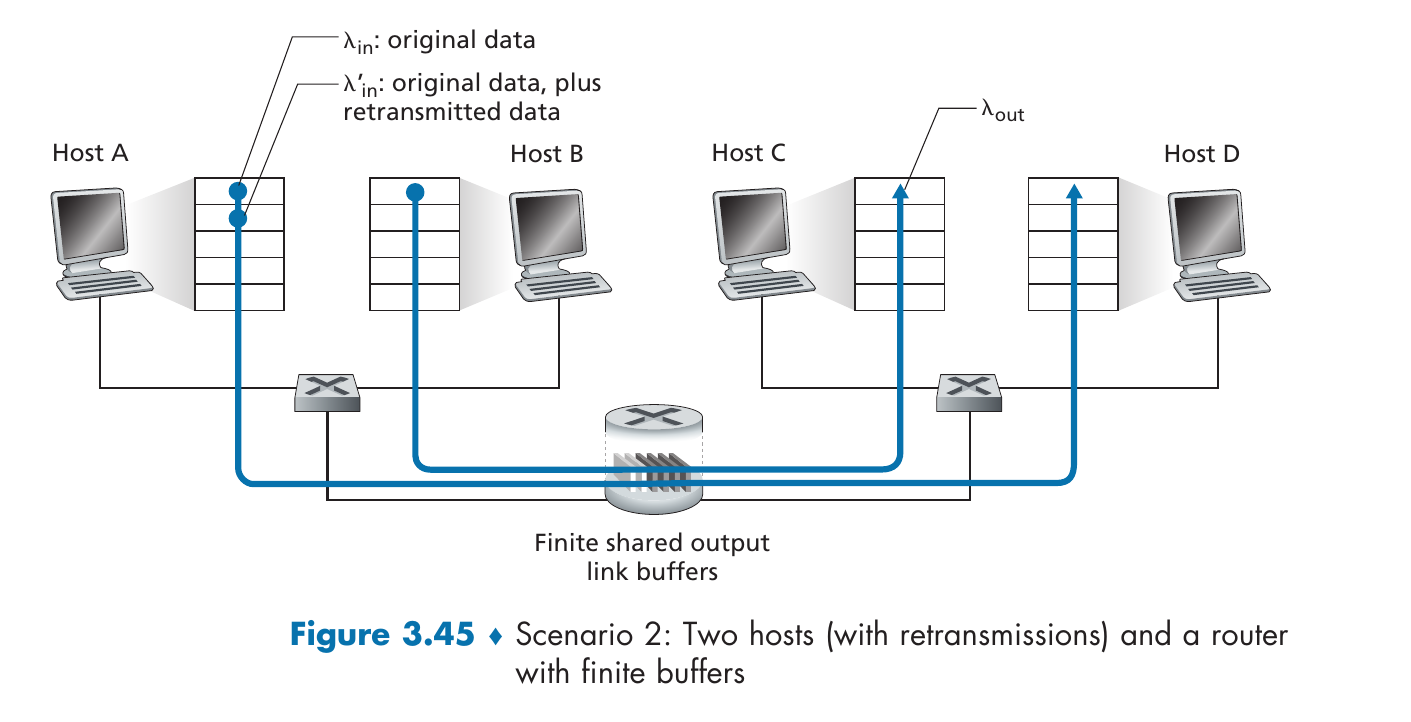
\includegraphics[width=0.55\linewidth]{cap12/scenario2.png}
    \caption{Lo stesso scenario con un buffer finito: i pacchetti in eccesso vengono scartati e i mittenti ritrasmettono.}
\end{figure}

Poiché il buffer è finito, i pacchetti accumulati prima o poi vengono \textbf{scartati}, e gli host devono
\textbf{ritrasmetterli}: altro traffico che si aggiunge a quello già eccessivo. Ora la velocità offerta alla rete
$\lambda'_{in}$ comprende dati originali e ritrasmissioni.

\begin{figure}[H]
    \centering
    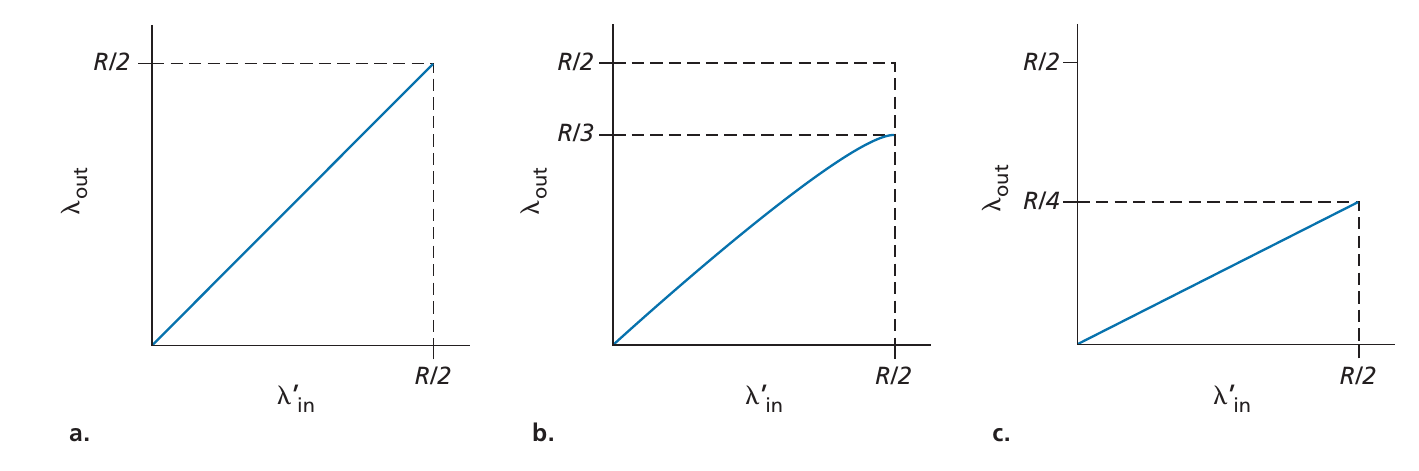
\includegraphics[width=0.6\linewidth]{cap12/scenario2_grafici.png}
    \caption{(a) Ritrasmissioni solo dei pacchetti davvero persi: si arriva a $R/2$. (b) Parte della capacità va in ritrasmissioni: il throughput utile scende (per esempio a $R/3$). (c) Con timeout prematuri si ritrasmettono anche pacchetti non persi: il throughput utile scende ancora (per esempio a $R/4$).}
\end{figure}

\warning{I costi della congestione}{
    \begin{itemize}
      \item \textbf{Ritardi} di accodamento elevati quando la velocità di arrivo si avvicina alla capacità.
      \item Il mittente deve \textbf{ritrasmettere} i pacchetti scartati, sprecando capacità.
      \item Timeout prematuri causano ritrasmissioni di pacchetti \textbf{non persi}: altro spreco.
      \item Un pacchetto scartato a metà cammino ha sprecato la capacità di tutti i collegamenti già attraversati.
    \end{itemize}
}

% ══════════════════════════════════════════════════════════════
\section{I due approcci al controllo di congestione}
% ══════════════════════════════════════════════════════════════

\begin{enumerate}
    \item \textbf{Controllo end-to-end}: è l'approccio standard di TCP. La congestione è \textbf{dedotta} dai sistemi
          terminali osservando il comportamento della rete (perdite, ritardi), senza alcun aiuto dal livello di rete.
          La perdita di un segmento (timeout o 3 ACK duplicati) è presa come segnale di congestione, e TCP riduce la
          velocità di invio.
    \item \textbf{Controllo assistito dalla rete}: approccio più recente e facoltativo, in cui trasporto e rete
          collaborano. I \textbf{router} forniscono un riscontro esplicito sullo stato di congestione a mittente e/o
          ricevente. Si usano i flag \textbf{CWR} ed \textbf{ECE} dell'header TCP (\emph{Explicit Congestion
          Notification}). Il riscontro può essere un semplice bit che indica congestione su un collegamento, o qualcosa
          di più sofisticato.
\end{enumerate}

% ══════════════════════════════════════════════════════════════
\section{Il controllo di congestione di TCP}
% ══════════════════════════════════════════════════════════════

TCP usa soprattutto il controllo \textbf{end-to-end}: ogni mittente adatta la propria velocità alla
congestione che percepisce. I problemi da risolvere sono tre:

\begin{enumerate}
    \item \textbf{Regolazione del ritmo}: come fa il mittente a limitare la velocità a cui immette traffico nella connessione?
    \item \textbf{Rilevazione della congestione}: come fa ad accorgersi che c'è congestione tra sé e la destinazione?
    \item \textbf{Aggiustamento del ritmo}: con quale algoritmo cambia la velocità in funzione della congestione percepita?
\end{enumerate}

\subsection{1. Regolazione del ritmo: la congestion window}

Nel controllo di flusso il ritmo è regolato dallo spazio del ricevente
($\text{LastByteSent} - \text{LastByteAcked} \leq \text{rwnd}$). Nel controllo di congestione il mittente
tiene anche una \textbf{finestra di congestione} (\emph{congestion window}, cwnd).

\dfn{Congestion window}{
    $$\text{LastByteSent} - \text{LastByteAcked} \leq \min\{\text{cwnd},\ \text{rwnd}\}$$
    Il ritmo di invio viene regolato \textbf{aumentando o diminuendo cwnd}: più grande è la finestra, più byte si
    possono avere in volo, più veloce è la trasmissione.
}

\begin{figure}[H]
\centering
\begin{tikzpicture}[every node/.style={font=\scriptsize\sffamily}]
  \fill[lnet] (0,0) rectangle (3,0.6); \fill[llink] (3,0) rectangle (6,0.6); \fill[white] (6,0) rectangle (8,0.6); \fill[lphy] (8,0) rectangle (12,0.6);
  \foreach \x in {0,0.5,...,12} \draw (\x,0) -- (\x,0.6);
  \draw (0,0) rectangle (12,0.6);
  \node[above] at (1.5,0.6) {inviati e confermati}; \node[above] at (4.5,0.6) {inviati, non confermati};
  \node[above] at (7,0.6) {inviabili}; \node[above] at (10,0.6) {non inviabili};
  \draw[{Stealth}-{Stealth}, very thick, netred] (3,-0.3) -- node[below, text=netred] {cwnd} (8,-0.3);
  \draw[{Stealth}-{Stealth}, very thick, netblue] (3,-0.9) -- node[below, text=netblue] {rwnd} (10,-0.9);
  \node[anchor=west, text width=4cm] at (12.3,-0.6) {la finestra effettiva è la più piccola delle due};
\end{tikzpicture}
\caption{Congestion window e receive window: comanda la più restrittiva.}
\end{figure}

\subsection{2. Rilevazione della congestione: i loss event}

\dfn{Loss event}{
    Il mittente TCP percepisce la congestione attraverso gli \textbf{eventi di perdita} (\emph{loss event}):
    \begin{itemize}
      \item la scadenza di un \textbf{timeout};
      \item la ricezione di \textbf{3 ACK duplicati}.
    \end{itemize}
    Entrambi indicano che un pacchetto precedente non è arrivato, probabilmente per il traboccare di un buffer in rete.
}

\begin{itemize}
    \item Se \textbf{non} ci sono eventi di perdita, cioè gli ACK arrivano come previsto, TCP assume che la rete non
          sia congestionata e \textbf{aumenta} cwnd. Gli ACK che arrivano fanno da ``orologio'': più arrivano in
          fretta, più in fretta cresce la finestra (TCP è \emph{self-clocking}).
    \item Se ci sono eventi di perdita, cwnd va \textbf{diminuita}.
\end{itemize}

\subsection{3. Aggiustamento del ritmo: l'algoritmo di Jacobson}

L'aggiustamento avviene tramite il \textbf{sondaggio della banda} (\emph{bandwidth probing}): il ritmo
cresce finché gli ACK arrivano correttamente (si ``tasta'' la rete), e quando si rileva congestione
(eventi di perdita) il ritmo viene ridotto. Il processo si ripete all'infinito.

TCP usa l'algoritmo di controllo di congestione di \textbf{Jacobson} (1988), con tre fasi:

\begin{enumerate}
    \item \textbf{Slow start}: si parte da 1 MSS e la velocità cresce \textbf{esponenzialmente}.
    \item \textbf{Additive increase} (o \emph{congestion avoidance}): la velocità cresce \textbf{linearmente}.
    \item \textbf{Fast recovery} (facoltativa): dopo 3 ACK duplicati si \textbf{dimezza} la velocità invece di
          ripartire da capo, e si prosegue con l'incremento lineare.
\end{enumerate}

% ══════════════════════════════════════════════════════════════
\section{Le fasi dell'algoritmo}
% ══════════════════════════════════════════════════════════════

\subsection{Slow start}

\dfn{Slow start}{
    All'inizio della connessione $\text{cwnd} = 1$ MSS. Per ogni ACK ricevuto cwnd aumenta di 1 MSS: così la finestra
    \textbf{raddoppia a ogni RTT} (1, 2, 4, 8, \dots). Nonostante il nome, la crescita è esponenziale: ``lento'' è solo il
    punto di partenza.
}

\begin{figure}[H]
\centering
\begin{tikzpicture}[yscale=0.62, every node/.style={font=\scriptsize\sffamily}]
  \timeline{a}{0}{Host A}{8.2}
  \timeline{b}{4}{Host B}{8.2}
  \draw[msg, netblue] (0,-0.2) -- node[above, sloped] {1 segmento} (4,-0.9);
  \draw[msg, netgreen] (4,-1.0) -- (0,-1.7);
  \draw[msg, netblue] (0,-1.9) -- (4,-2.6); \draw[msg, netblue] (0,-2.2) -- node[below, sloped] {2 segmenti} (4,-2.9);
  \draw[msg, netgreen] (4,-3.0) -- (0,-3.7); \draw[msg, netgreen] (4,-3.3) -- (0,-4.0);
  \foreach \k in {0,1,2,3} \draw[msg, netblue] (0,-4.2-\k*0.3) -- (4,-4.9-\k*0.3);
  \node[text=netblue] at (2.5,-6.3) {4 segmenti};
  \node[anchor=east] at (-0.3,-0.2) {cwnd = 1}; \node[anchor=east] at (-0.3,-1.9) {cwnd = 2}; \node[anchor=east] at (-0.3,-4.2) {cwnd = 4};
  \draw[decorate, decoration={brace, amplitude=4pt}] (4.3,-0.2) -- (4.3,-1.9) node[midway, right=5pt] {1 RTT};
\end{tikzpicture}
\caption{Slow start: ogni ACK fa crescere cwnd di 1 MSS, quindi la finestra raddoppia a ogni RTT.}
\end{figure}

La crescita esponenziale termina quando:

\begin{itemize}
    \item si verifica un \textbf{timeout}: si pone $\text{ssthresh} = \text{cwnd}/2$ (la \emph{slow start threshold},
          soglia di slow start), $\text{cwnd} = 1$ MSS, e si ricomincia lo slow start;
    \item cwnd raggiunge \textbf{ssthresh}: si passa in \textbf{congestion avoidance}, perché continuare a raddoppiare
          sarebbe imprudente;
    \item arrivano \textbf{3 ACK duplicati}: si esegue la ritrasmissione veloce e si entra in \textbf{fast recovery}.
\end{itemize}

\subsection{Congestion avoidance}

\dfn{Congestion avoidance (additive increase)}{
    Invece di raddoppiare, cwnd cresce di \textbf{1 MSS per ogni RTT} (in pratica, di
    $\text{MSS}\cdot\frac{\text{MSS}}{\text{cwnd}}$ per ogni ACK ricevuto). La crescita è \textbf{lineare}.
}

\begin{itemize}
    \item Se scade un \textbf{timeout}: come nello slow start, $\text{ssthresh} = \text{cwnd}/2$, $\text{cwnd} = 1$ MSS, e si torna in slow start.
    \item Se arrivano \textbf{3 ACK duplicati}: la rete riesce ancora a consegnare qualche segmento (gli ACK arrivano),
          quindi la reazione è meno drastica: $\text{ssthresh} = \text{cwnd}/2$, $\text{cwnd} = \text{ssthresh} + 3$ MSS
          (i tre segmenti che hanno generato i duplicati sono usciti dalla rete), e si entra in \textbf{fast recovery}.
\end{itemize}

\subsection{Fast recovery}

\dfn{Fast recovery}{
    In \textbf{fast recovery} cwnd aumenta di 1 MSS per ogni ulteriore ACK duplicato ricevuto per il segmento
    mancante. Quando arriva l'ACK del segmento perso, si pone $\text{cwnd} = \text{ssthresh}$ e si torna in
    \textbf{congestion avoidance}. Se invece scade un timeout, si torna in slow start con $\text{cwnd} = 1$ MSS.
}

\info{Tahoe e Reno}{
    La prima versione di TCP con controllo di congestione, \textbf{TCP Tahoe}, non aveva la fast recovery: dopo
    \emph{qualsiasi} evento di perdita ripartiva da $\text{cwnd} = 1$ MSS. \textbf{TCP Reno} ha introdotto la fast
    recovery, che dopo 3 ACK duplicati dimezza la finestra invece di azzerarla.
}

\begin{figure}[H]
\centering
\begin{tikzpicture}
  \begin{axis}[width=12cm, height=6.2cm, xlabel={tempo (RTT)}, ylabel={cwnd (in MSS)}, xmin=0.5, xmax=15.5, ymin=0, ymax=16,
      xtick={1,...,15}, ytick={0,2,...,16}, grid=major, grid style={gray!20}, legend pos=north west,
      legend style={font=\scriptsize\sffamily}, tick label style={font=\scriptsize}, label style={font=\footnotesize\sffamily}]
    \addplot[very thick, netred, mark=*, mark size=1.5pt] coordinates {(1,1) (2,2) (3,4) (4,8) (5,9) (6,10) (7,11) (8,12) (9,1) (10,2) (11,4) (12,6) (13,7) (14,8) (15,9)};
    \addlegendentry{TCP Tahoe}
    \addplot[very thick, netblue, mark=square*, mark size=1.5pt] coordinates {(1,1) (2,2) (3,4) (4,8) (5,9) (6,10) (7,11) (8,12) (9,9) (10,10) (11,11) (12,12) (13,13) (14,14) (15,15)};
    \addlegendentry{TCP Reno}
    \addplot[dashed, black!60, domain=0.5:8.5] {8};
    \addplot[dashed, black!60, domain=8.5:15.5] {6};
    \node[font=\scriptsize\sffamily, anchor=south west] at (axis cs:0.6,8) {ssthresh = 8};
    \node[font=\scriptsize\sffamily, anchor=north east] at (axis cs:15.4,6) {ssthresh = 6};
    \draw[-{Stealth}, thick] (axis cs:8,14.5) -- (axis cs:8,12.6);
    \node[font=\scriptsize\sffamily, anchor=south] at (axis cs:8,14.5) {3 ACK duplicati};
  \end{axis}
\end{tikzpicture}
\caption{Evoluzione di cwnd. Slow start fino a ssthresh = 8, poi crescita lineare. All'RTT 8 (cwnd = 12) arrivano 3 ACK duplicati: ssthresh diventa 6. Tahoe riparte da 1 MSS; Reno riparte da $6 + 3 = 9$ MSS e prosegue linearmente.}
\end{figure}

% ══════════════════════════════════════════════════════════════
\section{La macchina a stati del controllo di congestione}
% ══════════════════════════════════════════════════════════════

\begin{figure}[H]
\centering
\begin{tikzpicture}[every node/.style={font=\scriptsize\sffamily}, st/.style={circle, draw, thick, fill=cloudbg, minimum size=2.2cm, align=center, font=\footnotesize\bfseries\sffamily}]
  \node[st] (ss) at (0,0) {slow\\start};
  \node[st] (ca) at (9,0) {congestion\\avoidance};
  \node[st] (fr) at (4.5,-5.2) {fast\\recovery};
  \draw[-{Stealth}, very thick] (-2.6,1.4) node[above, align=center] {inizio:\\cwnd = 1 MSS, ssthresh = 64 kB} -- (ss);
  \draw[-{Stealth}, thick] (ss) to[loop above, looseness=5] node[above, align=center] {nuovo ACK: cwnd = cwnd + MSS} (ss);
  \draw[-{Stealth}, thick] (ca) to[loop above, looseness=5] node[above, align=center] {nuovo ACK: cwnd = cwnd + MSS$\cdot$(MSS/cwnd)} (ca);
  \draw[-{Stealth}, thick] (fr) to[loop below, looseness=5] node[below, align=center] {ACK duplicato: cwnd = cwnd + MSS} (fr);
  \draw[-{Stealth}, thick, netgreen!60!black] ([yshift=0.3cm]ss.east) -- node[above, align=center] {cwnd $\geq$ ssthresh} ([yshift=0.3cm]ca.west);
  \draw[-{Stealth}, thick, netred] ([yshift=-0.3cm]ca.west) -- node[below, align=center] {timeout: ssthresh = cwnd/2,\\cwnd = 1 MSS} ([yshift=-0.3cm]ss.east);
  \draw[-{Stealth}, thick, netorange] (ss.south) -- node[left, align=right] {3 ACK duplicati:\\ssthresh = cwnd/2,\\cwnd = ssthresh + 3 MSS,\\ritrasmette il segmento} (fr.north west);
  \draw[-{Stealth}, thick, netorange] ([xshift=-0.3cm]ca.south) -- node[left, align=right, pos=0.35] {3 ACK duplicati:\\ssthresh = cwnd/2,\\cwnd = ssthresh + 3 MSS} (fr.north east);
  \draw[-{Stealth}, thick, netgreen!60!black] (fr.east) to[out=0, in=-90] node[right, align=left] {nuovo ACK:\\cwnd = ssthresh} ([xshift=0.4cm]ca.south);
  \draw[-{Stealth}, thick, netred] (fr.west) to[out=180, in=-90] node[left, align=right] {timeout:\\ssthresh = cwnd/2,\\cwnd = 1 MSS} ([xshift=-0.4cm]ss.south);
\end{tikzpicture}
\caption{Macchina a stati semplificata del controllo di congestione di TCP Reno.}
\end{figure}

\begin{figure}[H]
    \centering
    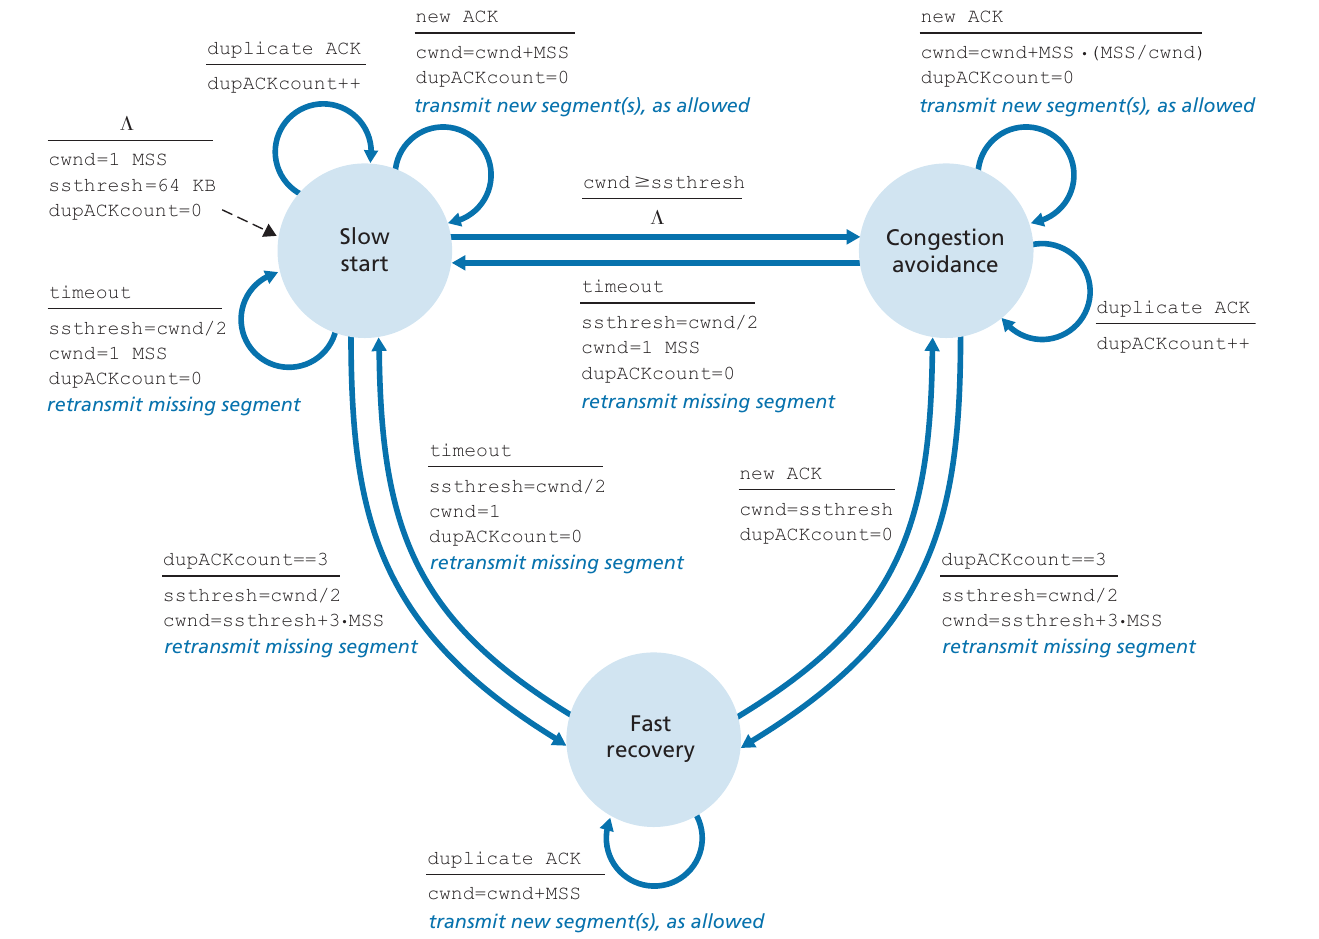
\includegraphics[width=0.62\linewidth]{cap12/fsm_congestione.png}
    \caption{La macchina a stati completa (Kurose), come mostrata a lezione.}
\end{figure}

\subsection{Il quadro completo delle transizioni}

\begin{table}[H]
\centering
\begin{tabular}{p{2.6cm}p{3.4cm}p{4.3cm}p{3.6cm}}
\toprule
\textbf{Stato} & \textbf{Evento} & \textbf{Azione} & \textbf{Nuovo stato} \\
\midrule
Slow start & nuovo ACK & cwnd += MSS & slow start (o CA se cwnd $\geq$ ssthresh) \\
Slow start & 3 ACK duplicati & ssthresh = cwnd/2; cwnd = ssthresh + 3 MSS; ritrasmissione & fast recovery \\
Slow start & timeout & ssthresh = cwnd/2; cwnd = 1 MSS; ritrasmissione & slow start \\
Congestion avoid. & nuovo ACK & cwnd += MSS$\cdot$MSS/cwnd & congestion avoidance \\
Congestion avoid. & 3 ACK duplicati & ssthresh = cwnd/2; cwnd = ssthresh + 3 MSS; ritrasmissione & fast recovery \\
Congestion avoid. & timeout & ssthresh = cwnd/2; cwnd = 1 MSS; ritrasmissione & slow start \\
Fast recovery & ACK duplicato & cwnd += MSS & fast recovery \\
Fast recovery & nuovo ACK & cwnd = ssthresh & congestion avoidance \\
Fast recovery & timeout & ssthresh = cwnd/2; cwnd = 1 MSS & slow start \\
\bottomrule
\end{tabular}
\caption{Tutte le transizioni del controllo di congestione di TCP Reno.}
\end{table}

\info{AIMD e il dente di sega}{
    Ignorando lo slow start iniziale e supponendo le perdite segnalate da 3 ACK duplicati, TCP aumenta cwnd di 1 MSS
    per RTT e la dimezza a ogni perdita: è l'approccio \textbf{AIMD} (\emph{Additive Increase, Multiplicative
    Decrease}). Il grafico di cwnd nel tempo ha la tipica forma a \textbf{dente di sega}. Se $W$ è la finestra a cui
    avviene la perdita, il throughput medio di una connessione è circa $\dfrac{0{,}75\cdot W}{\text{RTT}}$.
}

\begin{figure}[H]
\centering
\begin{tikzpicture}
  \begin{axis}[width=11cm, height=4.6cm, xlabel={tempo}, ylabel={cwnd}, xmin=0, xmax=24, ymin=0, ymax=26, xtick=\empty, ytick={12,24}, yticklabels={$W/2$, $W$},
      tick label style={font=\scriptsize}, label style={font=\footnotesize\sffamily}]
    \addplot[very thick, netblue] coordinates {(0,12) (6,24) (6,12) (12,24) (12,12) (18,24) (18,12) (24,24)};
    \addplot[dashed, netred, domain=0:24] {18};
    \node[font=\scriptsize\sffamily, text=netred, anchor=south east] at (axis cs:24,18) {media $\approx 0{,}75\,W$};
  \end{axis}
\end{tikzpicture}
\caption{Il dente di sega di AIMD: crescita lineare, dimezzamento a ogni perdita.}
\end{figure}

% ══════════════════════════════════════════════════════════════
\section{Analizzare il traffico TCP con Wireshark}
% ══════════════════════════════════════════════════════════════

\begin{esercizio}{Una connessione TCP con netcat}
\texttt{netcat} (\texttt{nc}) apre connessioni TCP o UDP ``a mano'', ed è ideale per osservare TCP con Wireshark sulla
propria macchina (interfaccia di \emph{loopback}, \texttt{127.0.0.1}).
\begin{lstlisting}[language=bash]
$ nc -l 5001                 # terminale 1: server in ascolto sulla porta 5001
$ nc localhost 5001          # terminale 2: client; ogni riga digitata viene inviata
\end{lstlisting}
In Wireshark, sull'interfaccia \texttt{lo}, si usa il filtro \texttt{tcp \&\& tcp.port==5001 \&\& ip}.
\begin{itemize}
    \item Si osservano il \textbf{three-way handshake} (SYN, SYN-ACK, ACK), i segmenti con le stringhe ASCII e gli
          \textbf{ACK senza dati} del server, e alla chiusura lo scambio di FIN.
    \item Si può poi inviare un file: \texttt{nc -l 12332 > real.doc} sul server e
          \texttt{nc 127.0.0.1 12332 < real.doc} sul client, osservando come il file viene spezzato in segmenti e come
          crescono numeri di sequenza e di acknowledgment.
\end{itemize}
\end{esercizio}

\begin{esercizio}{Uno scaricamento reale}
Si avvia la cattura e si scarica un file di prova, per esempio con
\texttt{wget http://speedtest.tele2.net/10MB.zip}.
\begin{itemize}
    \item Clic destro su un segmento dello scaricamento, \emph{Follow $\rightarrow$ TCP Stream}, per isolare la connessione.
    \item Filtri utili (svolgimento completo nella Parte VII):
          \begin{itemize}
            \item \texttt{tcp}: tutto il traffico TCP;
            \item \texttt{tcp.analysis.bytes\_in\_flight}: i byte in volo, legati alla finestra di congestione;
            \item \texttt{tcp.analysis.duplicate\_ack}: gli ACK duplicati;
            \item \texttt{tcp.analysis.window\_update}: gli aggiornamenti della finestra di ricezione.
          \end{itemize}
    \item Il menu \emph{Statistics $\rightarrow$ TCP Stream Graphs} mostra l'andamento dei numeri di sequenza nel tempo:
          si riconoscono lo slow start iniziale e i rallentamenti dopo le perdite.
\end{itemize}
\end{esercizio}

% ══════════════════════════════════════════════════════════════
\section{Riepilogo}
% ══════════════════════════════════════════════════════════════

\riepilogo{
\begin{itemize}
    \item \textbf{Flusso}: proteggere il ricevente. $\text{rwnd} = \text{RcvBuffer} - (\text{LastByteRcvd} - \text{LastByteRead})$;
          il mittente mantiene $\text{LastByteSent} - \text{LastByteAcked} \leq \text{rwnd}$.
    \item \textbf{Congestione}: proteggere la rete. Buffer infiniti $\Rightarrow$ ritardi infiniti; buffer finiti $\Rightarrow$
          perdite e ritrasmissioni che sprecano capacità.
    \item TCP usa il controllo \textbf{end-to-end}: $\text{LastByteSent} - \text{LastByteAcked} \leq \min\{\text{cwnd}, \text{rwnd}\}$.
    \item \textbf{Loss event}: timeout o 3 ACK duplicati.
    \item \textbf{Slow start} (cwnd raddoppia per RTT fino a ssthresh), \textbf{congestion avoidance} (+1 MSS per RTT),
          \textbf{fast recovery} (dopo 3 duplicati: ssthresh = cwnd/2, cwnd = ssthresh + 3); timeout $\Rightarrow$ cwnd = 1 MSS.
\end{itemize}
}
     % Flusso e congestione

  % ------------------------------------------------------------------
  \part{Il livello di rete}
  % ------------------------------------------------------------------
  \chapter{Il livello di rete e i router}

\begin{center}
\begin{tikzpicture}[node distance=0pt]
  \node[lay app, minimum width=3.4cm] (a) {Applicazione};
  \node[lay tra, minimum width=3.4cm, below=of a] (t) {Trasporto};
  \node[lay net, minimum width=3.4cm, below=of t, line width=1.5pt, draw=netred] (n) {\bfseries Rete};
  \node[lay link, minimum width=3.4cm, below=of n] (l) {Collegamento};
  \node[lay phy, minimum width=3.4cm, below=of l] (p) {Fisico};
  \draw[-{Stealth}, thick, netred] ([xshift=0.3cm]n.east) -- ++(1,0) node[right, lbl, text=netred] {siamo qui};
\end{tikzpicture}
\end{center}

% ══════════════════════════════════════════════════════════════
\section{Dal trasporto alla rete}
% ══════════════════════════════════════════════════════════════

Il compito del livello di rete è permettere a host remoti di comunicare:

\begin{itemize}
    \item \textbf{sull'host mittente}: prendere i segmenti dal livello di trasporto, incapsulare ciascuno in un
          \textbf{datagramma} e inviare i datagrammi nella rete;
    \item \textbf{sull'host ricevente}: ricevere i datagrammi dalla rete, estrarne i segmenti di trasporto e
          consegnarli al livello di trasporto.
\end{itemize}

A questo livello lavorano alcuni dei protocolli più importanti delle reti (IP, DHCP, NAT, ICMP, i protocolli di
routing) e dispositivi speciali: i \textbf{router}.

\begin{figure}[H]
\centering
\begin{minipage}{0.45\linewidth}\centering
  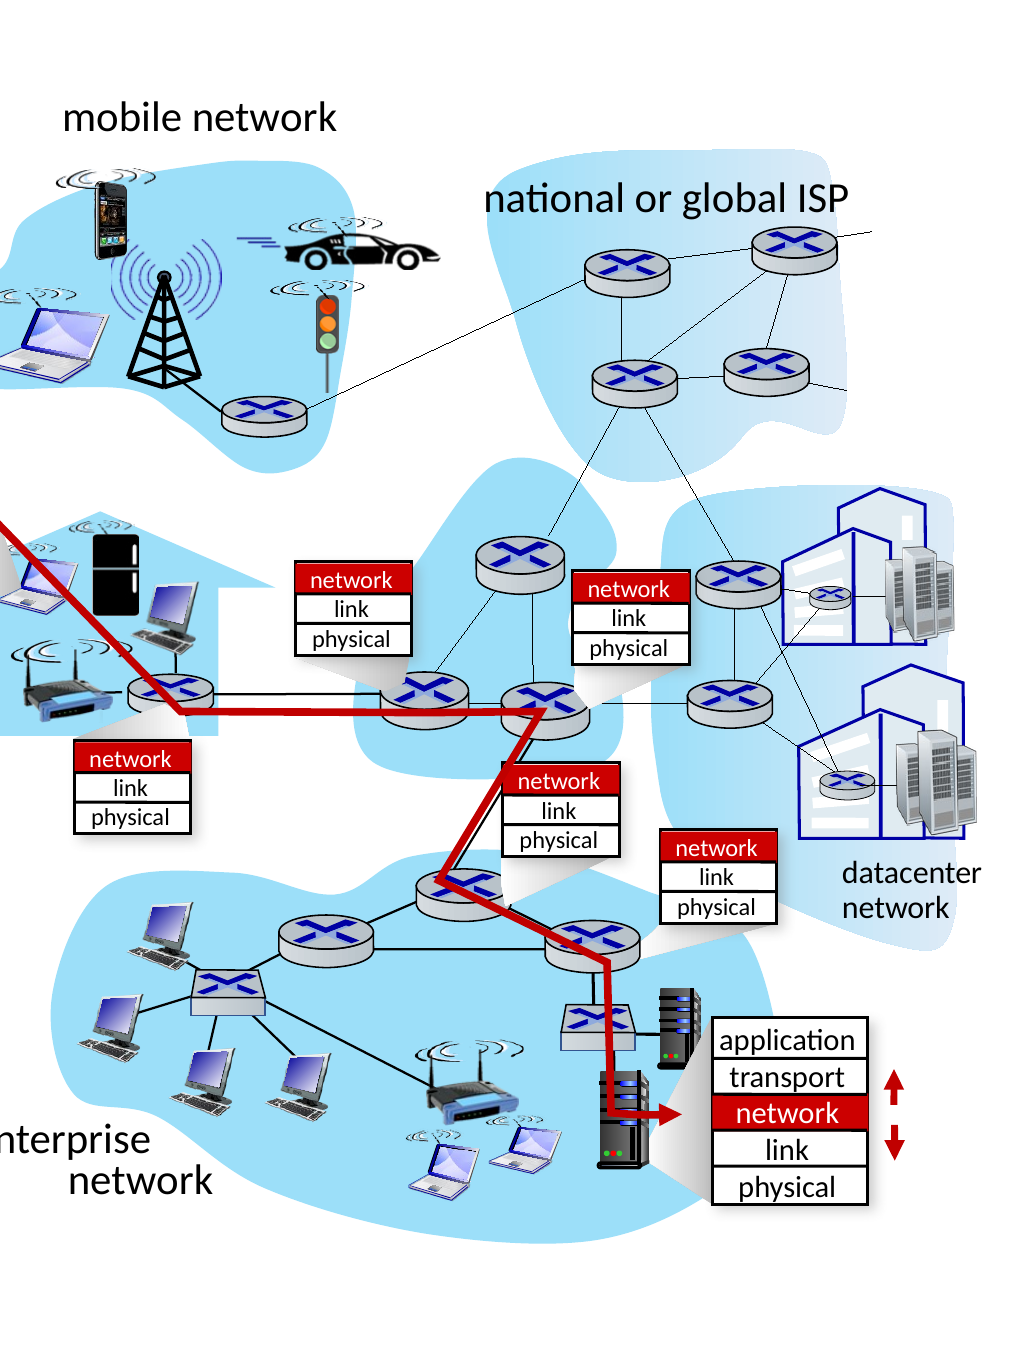
\includegraphics[width=0.9\linewidth]{cap13/stack_troncato.png}
\end{minipage}\hfill
\begin{minipage}{0.51\linewidth}
All'interno della rete ci sono nodi, i \textbf{router}, che inoltrano i datagrammi ai nodi adiacenti fino all'host
di destinazione.
\begin{itemize}
  \item Nelle figure i router hanno una \textbf{pila troncata} (rete, collegamento, fisico): non eseguono applicazioni
        né protocolli di trasporto.
  \item L'atto di un datagramma che viene reindirizzato da un router si chiama \textbf{hop} (salto).
\end{itemize}
\end{minipage}
\caption{Solo gli host hanno la pila completa; i router si fermano al livello di rete.}
\end{figure}

\begin{figure}[H]
\centering
\begin{tikzpicture}[every node/.style={font=\scriptsize\sffamily}]
  \begin{scope}
    \node[lay app, minimum width=1.8cm] at (0,2.4) {applicazione};
    \node[lay tra, minimum width=1.8cm] at (0,1.8) {trasporto};
    \node[lay net, minimum width=1.8cm] at (0,1.2) {rete};
    \node[lay link, minimum width=1.8cm] at (0,0.6) {collegamento};
    \node[lay phy, minimum width=1.8cm] at (0,0) {fisico};
    \node at (0,-0.6) {\icon[0.7cm]{pc}};
  \end{scope}
  \foreach \x/\n in {3.6/1, 7.2/2} {
    \begin{scope}[xshift=\x cm]
      \node[lay net, minimum width=1.8cm] at (0,1.2) {rete};
      \node[lay link, minimum width=1.8cm] at (0,0.6) {collegamento};
      \node[lay phy, minimum width=1.8cm] at (0,0) {fisico};
      \node at (0,-0.6) {\icon[0.9cm]{router}};
    \end{scope}
  }
  \begin{scope}[xshift=10.8cm]
    \node[lay app, minimum width=1.8cm] at (0,2.4) {applicazione};
    \node[lay tra, minimum width=1.8cm] at (0,1.8) {trasporto};
    \node[lay net, minimum width=1.8cm] at (0,1.2) {rete};
    \node[lay link, minimum width=1.8cm] at (0,0.6) {collegamento};
    \node[lay phy, minimum width=1.8cm] at (0,0) {fisico};
    \node at (0,-0.6) {\icon[0.4cm]{server}};
  \end{scope}
  \draw[-{Stealth}, very thick, netred] (0,2.1) -- (0,-0.25) -- (2.6,-0.25) -- (2.6,1.2) -- (4.6,1.2) -- (4.6,-0.25) -- (6.2,-0.25) -- (6.2,1.2) -- (8.2,1.2) -- (8.2,-0.25) -- (9.8,-0.25) -- (9.8,2.1);
  \node[text=netred] at (1.8,-1.1) {hop 1}; \node[text=netred] at (5.4,-1.1) {hop 2}; \node[text=netred] at (9,-1.1) {hop 3};
\end{tikzpicture}
\caption{Il datagramma sale fino al livello di rete in ogni router, che decide dove inoltrarlo, e riscende.}
\end{figure}

% ══════════════════════════════════════════════════════════════
\section{Che servizi offre il livello di rete}
% ══════════════════════════════════════════════════════════════

Il livello di rete è responsabile della \textbf{consegna host-a-host}. In teoria, insieme alla consegna potrebbe
offrire servizi come:

\begin{itemize}
    \item \textbf{consegna garantita}: un pacchetto inviato arriverà prima o poi a destinazione;
    \item \textbf{consegna garantita con ritardo limitato}: arriverà entro un certo tempo (per esempio 100 ms);
    \item \textbf{consegna in ordine}: i pacchetti arrivano nell'ordine di invio;
    \item \textbf{banda minima garantita}: se il mittente non supera una certa velocità (per esempio 1 Mb/s), tutti i
          pacchetti arrivano;
    \item \textbf{sicurezza}: cifratura e decifratura di tutti i datagrammi.
\end{itemize}

In realtà, \textbf{nessuno} di questi servizi è offerto in generale dalle reti.

\dfn{Servizio best effort}{
    Il livello di rete di Internet offre un solo servizio, detto \textbf{best effort} (``del proprio meglio''): la
    rete \textbf{fa del suo meglio} per consegnare un pacchetto dalla sorgente alla destinazione, ma non garantisce
    né che arrivi, né che arrivi in ordine, né ritardi massimi, né banda minima.
}

Nonostante la sua semplicità, il modello best effort, insieme a una buona disponibilità di banda, si è
dimostrato \textbf{adeguato}: Netflix, le videochiamate, le conferenze in tempo reale funzionano tutte così.

% ══════════════════════════════════════════════════════════════
\section{I router nella rete}
% ══════════════════════════════════════════════════════════════

I router sono nodi speciali con \textbf{più collegamenti in ingresso e in uscita}. Offrono due funzioni di rete
fondamentali.

\dfn{Forwarding e routing}{
    \begin{itemize}
      \item \textbf{Forwarding} (inoltro): quando un pacchetto arriva su un collegamento di ingresso, il router lo
            sposta sul \textbf{collegamento di uscita} appropriato. È un'azione \textbf{locale} al router.
      \item \textbf{Routing} (instradamento): decidere il \textbf{percorso} che i pacchetti devono seguire dalla
            sorgente alla destinazione. È un processo che riguarda \textbf{tutta la rete}; gli algoritmi che
            calcolano i percorsi sono gli \textbf{algoritmi di routing}.
    \end{itemize}
}

Durante il forwarding un router può anche:

\begin{enumerate}
    \item \textbf{bloccare} un pacchetto (se proviene da un host noto come malevolo o è diretto a un host vietato);
    \item \textbf{scartare} un pacchetto scaduto;
    \item \textbf{duplicare} un pacchetto e inviarlo su più collegamenti;
    \item \textbf{modificare} un pacchetto (per esempio per segnalare congestione).
\end{enumerate}

\info{L'analogia del viaggio in auto}{
    Il \textbf{routing} è pianificare il viaggio da Napoli a Milano, scegliendo le autostrade da percorrere. Il
    \textbf{forwarding} è quello che si fa a ogni svincolo: guardare il cartello e imboccare l'uscita giusta. Il primo
    richiede una visione d'insieme e si fa una volta; il secondo è rapido, locale e si ripete a ogni incrocio.
}

\begin{figure}[H]
\centering
\begin{tikzpicture}[every node/.style={font=\footnotesize\sffamily}]
  \begin{scope}
    \node[font=\small\bfseries\sffamily] at (1.5,1.6) {Forwarding};
    \node (r) at (1.5,0) {\icon[1.3cm]{router}};
    \draw[msg, very thick, netblue] (-0.8,0.5) -- node[above] {P} (0.8,0.1);
    \draw[msg, very thick, netgreen] (2.2,0.1) -- (3.8,0.9); \draw[thick, black!30] (2.2,-0.1) -- (3.8,-0.8); \draw[thick, black!30] (0.8,-0.2) -- (-0.8,-0.8);
    \node[below=4pt of r, text width=3cm, align=center] {sposta il pacchetto dall'ingresso all'uscita giusta};
  \end{scope}
  \begin{scope}[xshift=7cm]
    \node[font=\small\bfseries\sffamily] at (2.5,1.6) {Routing};
    \foreach \x/\y [count=\i] in {0/0, 1.5/0.9, 1.6/-0.9, 3.2/0.6, 3.3/-0.7, 4.8/0} \node (n\i) at (\x,\y) {\icon[0.7cm]{router}};
    \foreach \a/\b in {1/2, 1/3, 2/4, 3/5, 2/5, 4/6, 5/6, 3/4} \draw[thick, black!30] (n\a) -- (n\b);
    \draw[pathhl, -{Stealth}] (n1) -- (n2) -- (n4) -- (n6);
    \node[text width=4.6cm, align=center] at (2.4,-1.8) {calcola il percorso migliore attraverso tutta la rete};
  \end{scope}
\end{tikzpicture}
\caption{Forwarding (locale) e routing (globale).}
\end{figure}

% ══════════════════════════════════════════════════════════════
\section{Tipi di router}
% ══════════════════════════════════════════════════════════════

\begin{figure}[H]
\centering
\begin{minipage}{0.4\linewidth}\centering
  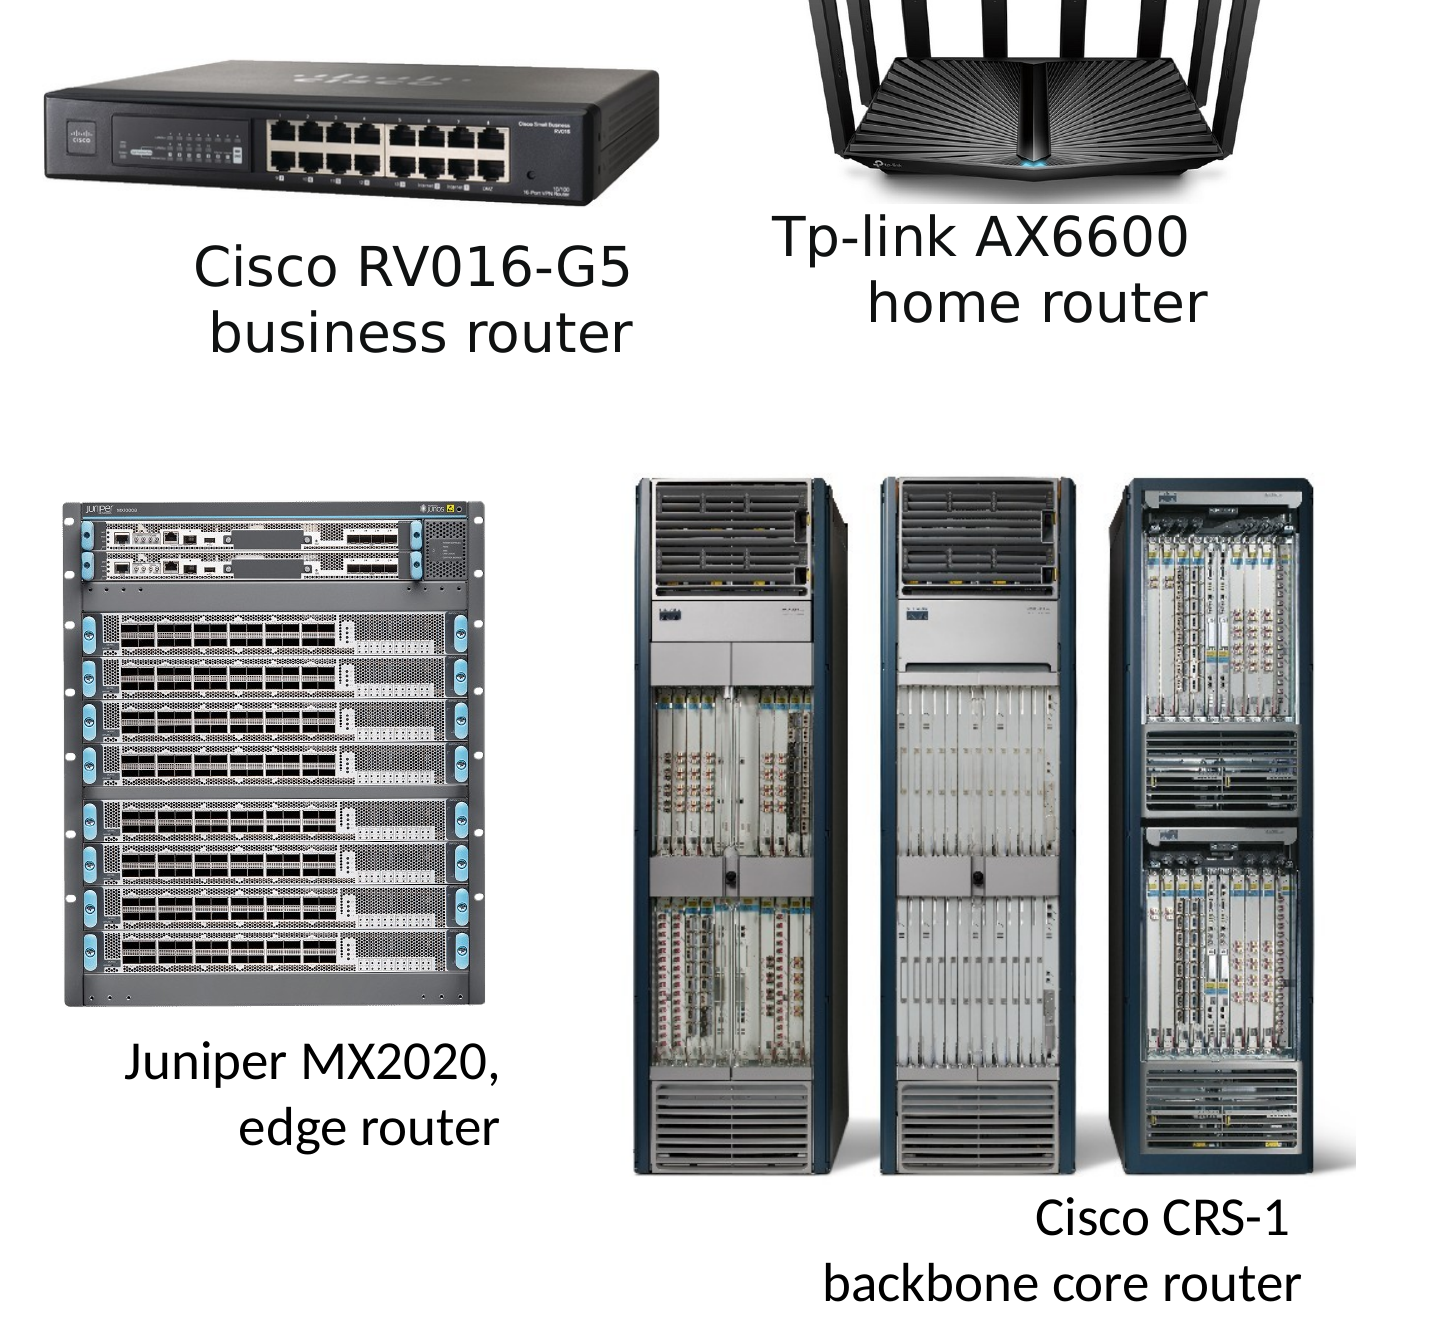
\includegraphics[width=0.95\linewidth]{cap13/router_foto.png}
\end{minipage}\hfill
\begin{minipage}{0.56\linewidth}
I router possono essere molto diversi a seconda di uso e tecnologia: per casa o per ufficio, con o senza fili.
Una distinzione importante è quella tra:
\begin{itemize}
  \item \textbf{edge router} (router di bordo): distribuiscono pacchetti \textbf{tra reti diverse}, per esempio
        collegando una rete con l'ISP. È il tipo più comune;
  \item \textbf{core router} (router di nucleo): distribuiscono pacchetti \textbf{all'interno di una stessa rete}.
        Sono usati anche sulla dorsale (\emph{backbone}) di Internet, dove devono smaltire trasferimenti di dati enormi.
\end{itemize}
\end{minipage}
\caption{Router per uso domestico e aziendale (in alto), un edge router e un core router da dorsale (in basso).}
\end{figure}

% ══════════════════════════════════════════════════════════════
\section{Data plane e control plane}
% ══════════════════════════════════════════════════════════════

\dfn{I due piani di un router}{
    \begin{itemize}
      \item Il \textbf{data plane} (piano dei dati, o di forwarding) comprende l'azione locale di trasferire un
            pacchetto da un'interfaccia di ingresso a quella di uscita appropriata. È un'operazione \textbf{veloce}
            (pochi nanosecondi), di solito realizzata in \textbf{hardware}.
      \item Il \textbf{control plane} (piano di controllo) comprende il processo, esteso a tutta la rete, che
            determina i percorsi da un estremo all'altro. È più \textbf{lento} (secondi), e spesso realizzato in
            \textbf{software}.
    \end{itemize}
}

Nel data plane c'è la \textbf{forwarding table} (tabella di inoltro): una tabella che associa gli indirizzi di
destinazione ai collegamenti di uscita. Il router inoltra un pacchetto esaminando uno o più campi del suo
header; il valore trovato nella tabella indica l'interfaccia su cui inoltrarlo.

\warning{La tabella non contiene i singoli indirizzi}{
    Una forwarding table \textbf{non} elenca gli indirizzi dei singoli host (sarebbero miliardi): associa alle porte
    di uscita \textbf{gruppi di indirizzi}, cioè intervalli individuati da un prefisso (le \emph{subnet}).
}

\subsection{Centralizzato o decentralizzato}

Poiché prima di arrivare a destinazione si attraversano molti router, il contenuto di una forwarding table va
determinato raccogliendo informazioni da router diversi. Lo si fa con una o più \textbf{tabelle di routing}
(control plane), da cui si ricava la forwarding table (data plane). Ci sono due modi:

\begin{figure}[H]
\centering
\begin{tikzpicture}[every node/.style={font=\scriptsize\sffamily}]
  \begin{scope}
    \node[font=\footnotesize\bfseries\sffamily] at (2.3,2.7) {Decentralizzato};
    \foreach \x [count=\i] in {0,1.5,3,4.5} {
      \node[draw, fill=lnet!40, minimum width=1.1cm, minimum height=0.5cm] (cp\i) at (\x,1.7) {routing};
      \node[draw, fill=llink!60, minimum width=1.1cm, minimum height=0.5cm] (dp\i) at (\x,0.9) {tabella};
      \draw[-{Stealth}] (cp\i) -- (dp\i);
      \node at (\x,0.1) {\icon[0.6cm]{router}};
    }
    \foreach \i/\j in {1/2, 2/3, 3/4} \draw[{Stealth}-{Stealth}, netred, thick] (cp\i) -- (cp\j);
    \node[text width=4.8cm, align=center] at (2.25,-0.7) {ogni router ha un componente di routing che dialoga con quelli degli altri};
  \end{scope}
  \begin{scope}[xshift=8cm]
    \node[font=\footnotesize\bfseries\sffamily] at (2.3,2.7) {Centralizzato (SDN)};
    \node[draw, fill=lnet!60, rounded corners, minimum width=4.8cm, minimum height=0.6cm] (ctrl) at (2.25,1.9) {controller remoto (software)};
    \foreach \x [count=\i] in {0,1.5,3,4.5} {
      \node[draw, fill=llink!60, minimum width=1.1cm, minimum height=0.5cm] (dp\i) at (\x,0.9) {tabella};
      \draw[-{Stealth}, netred, thick] (ctrl.south -| dp\i) -- (dp\i);
      \node at (\x,0.1) {\icon[0.6cm]{router}};
    }
    \node[text width=4.8cm, align=center] at (2.25,-0.7) {un controller separato calcola e distribuisce le tabelle di inoltro};
  \end{scope}
\end{tikzpicture}
\caption{Control plane decentralizzato e centralizzato.}
\end{figure}

\begin{itemize}
    \item \textbf{Decentralizzato} (distribuito): ogni router ha un componente di routing che comunica con i componenti
          di routing degli altri router. È stato a lungo l'approccio dominante.
    \item \textbf{Centralizzato}: un \textbf{controller remoto}, fisicamente separato dai router, calcola le tabelle e
          le distribuisce. Può trovarsi in un data center remoto, affidabile e ridondato, gestito dall'ISP o da terzi.
\end{itemize}

\info{Software-Defined Networking}{
    L'approccio centralizzato è alla base del \textbf{Software-Defined Networking} (SDN): la rete è ``definita dal
    software'' perché il controller che calcola le tabelle e dialoga con i router è un software centralizzato,
    talvolta anche open source.
}

% ══════════════════════════════════════════════════════════════
\section{Le componenti di un router}
% ══════════════════════════════════════════════════════════════

\begin{figure}[H]
\centering
\begin{tikzpicture}[every node/.style={font=\footnotesize\sffamily}]
  \draw[thick, rounded corners, fill=black!3] (-0.6,-3.3) rectangle (9.6,1.5);
  \node[anchor=north west, font=\small\bfseries\sffamily] at (-0.5,1.45) {Router};
  \foreach \y/\i in {0/1, -1.2/2, -2.6/N} {
    \node[draw, fill=lnet!40, minimum width=2cm, minimum height=0.8cm, align=center] (in\i) at (1,\y) {porta di\\ingresso \i};
    \node[draw, fill=llink!60, minimum width=2cm, minimum height=0.8cm, align=center] (out\i) at (8,\y) {porta di\\uscita \i};
    \draw[-{Stealth}, very thick] (-1.6,\y) -- (in\i.west);
    \draw[-{Stealth}, very thick] (out\i.east) -- (10.6,\y);
  }
  \node at (1,-1.9) {$\vdots$}; \node at (8,-1.9) {$\vdots$};
  \node[draw, fill=ltra!50, minimum width=2.4cm, minimum height=3.4cm, align=center] (sf) at (4.5,-1.3) {switching\\fabric};
  \foreach \i in {1,2,N} { \draw[-{Stealth}, thick] (in\i.east) -- (in\i.east -| sf.west); \draw[-{Stealth}, thick] (out\i.west -| sf.east) -- (out\i.west); }
  \node[draw, fill=lapp!50, rounded corners, minimum width=3cm, align=center] (rp) at (4.5,2.4) {processore di routing\\(control plane)};
  \draw[{Stealth}-{Stealth}, dashed, thick, netred] (rp.south) -- node[right, text=netred] {tabelle} (sf.north);
  \draw[-{Stealth}, dashed, netred] (rp.west) -| (in1.north);
  \node[anchor=east] at (-1.7,-1.3) {collegamenti di ingresso};
  \node[anchor=west, text width=2cm] at (10.7,-1.3) {collegamenti di uscita};
  \node[text=black!60] at (4.5,-3.0) {data plane (hardware)};
\end{tikzpicture}
\caption{Architettura di un router.}
\end{figure}

\begin{itemize}
    \item \textbf{Porte di ingresso} (da non confondere con le porte del trasporto): sono le interfacce fisiche
          collegate ai collegamenti in ingresso. Il loro compito è:
    \begin{itemize}
      \item consultare la forwarding table (\emph{lookup}) e preparare la switching fabric verso la porta di uscita scelta;
      \item inoltrare al processore di routing i pacchetti di controllo (per esempio quelli con le informazioni di routing).
    \end{itemize}
    Il numero di porte va da decine a centinaia (l'edge router Juniper MX2020 supporta fino a 960 porte Ethernet da 10 Gb/s).
    \item \textbf{Switching fabric} (matrice di commutazione): collega le porte di ingresso a quelle di uscita.
    \item \textbf{Porte di uscita}: conservano i pacchetti ricevuti dalla switching fabric e li trasmettono sul
          collegamento in uscita. Le porte possono essere bidirezionali (ingresso e uscita accoppiati).
    \item \textbf{Processore di routing}: esegue i protocolli di routing, mantiene informazioni sullo stato dei
          collegamenti e calcola e aggiorna la forwarding table.
\end{itemize}

% ══════════════════════════════════════════════════════════════
\section{Il forwarding e la longest prefix matching}
% ══════════════════════════════════════════════════════════════

La forwarding table associa \textbf{indirizzi IP} a \textbf{porte di uscita}, così che i pacchetti possano essere
inoltrati sul collegamento giusto verso il nodo successivo (dove, eventualmente, verranno inoltrati di nuovo).

Un indirizzo IP è un numero di \textbf{4 byte} (32 bit), che di solito si scrive in notazione decimale ma che si può
vedere in binario:

\begin{center}
\begin{tabular}{ll}
decimale puntata & \texttt{192.168.1.1} \\
binario & \texttt{11000000 10101000 00000001 00000001} \\
\end{tabular}
\end{center}

Quando un pacchetto arriva su una porta di ingresso si esegue un \textbf{lookup}. Ogni porta ha una
\textbf{copia} della forwarding table, ricevuta dal processore di routing su un bus dedicato (per esempio PCI), per
evitare il collo di bottiglia di interrogare il processore per ogni pacchetto. Più indirizzi possono essere
associati alla stessa porta.

\begin{table}[H]
\centering
\begin{tabular}{llc}
\toprule
\textbf{Prefisso degli indirizzi} & \textbf{Intervallo di indirizzi corrispondente} & \textbf{Interfaccia} \\
\midrule
\texttt{11001000 00010111 00010*** ********} & da \texttt{...00010000 00000000} a \texttt{...00010111 11111111} & 0 \\
\texttt{11001000 00010111 00011000 ********} & da \texttt{...00011000 00000000} a \texttt{...00011000 11111111} & 1 \\
\texttt{11001000 00010111 00011*** ********} & da \texttt{...00011000 00000000} a \texttt{...00011111 11111111} & 2 \\
altrimenti & & 3 \\
\bottomrule
\end{tabular}
\caption{Una forwarding table a 4 porte: ogni riga è un prefisso, cioè un intervallo di indirizzi (i primi 16 bit sono sempre \texttt{11001000 00010111}).}
\end{table}

\warning{Righe che si sovrappongono}{
    Le righe non sono necessariamente mutuamente esclusive. Per esempio l'indirizzo
    \texttt{11001000 00010111 00011000 10101010} corrisponde sia alla riga dell'interfaccia 1 sia a quella
    dell'interfaccia 2. A quale porta va?
}

\dfn{Longest prefix matching}{
    Se un indirizzo corrisponde a più righe della forwarding table, il router lo inoltra verso la porta associata alla
    riga con il \textbf{prefisso più lungo} (\emph{longest prefix matching rule}).
}

\begin{figure}[H]
\centering
\begin{tikzpicture}[every node/.style={font=\small\ttfamily}]
  \node[anchor=west] (addr) at (0,0) {\textcolor{netred}{11001000 00010111 00011000} 10101010};
  \node[anchor=west, font=\small\sffamily] at (8,0) {indirizzo di destinazione};
  \draw[decorate, decoration={brace, amplitude=5pt}, netgreen!60!black, thick] (0.1,0.35) -- (6.05,0.35) node[midway, above=6pt, font=\footnotesize\sffamily, text=netgreen!50!black] {match con la riga dell'interfaccia 1: 24 bit};
  \draw[decorate, decoration={brace, amplitude=5pt, mirror}, netblue, thick] (0.1,-0.35) -- (5.35,-0.35) node[midway, below=6pt, font=\footnotesize\sffamily, text=netblue] {match con la riga dell'interfaccia 2: 21 bit};
  \node[font=\small\bfseries\sffamily, text=netgreen!50!black] at (10,-1.1) {vince l'interfaccia 1!};
\end{tikzpicture}
\caption{Longest prefix matching: tra le righe che corrispondono si sceglie quella con il prefisso più lungo.}
\end{figure}

\begin{esempio}{Dove va il pacchetto?}
Con la tabella precedente:
\begin{itemize}
    \item \texttt{11001000 00010111 00010110 10100001}: corrisponde solo al prefisso \texttt{...00010} $\Rightarrow$ interfaccia \textbf{0};
    \item \texttt{11001000 00010111 00011000 10101010}: corrisponde a \texttt{...00011000} (24 bit) e a \texttt{...00011} (21 bit)
          $\Rightarrow$ interfaccia \textbf{1};
    \item \texttt{11001000 00010111 00011001 00000001}: corrisponde solo a \texttt{...00011} $\Rightarrow$ interfaccia \textbf{2};
    \item \texttt{11001000 00010111 00100000 00000001}: nessun prefisso $\Rightarrow$ interfaccia \textbf{3}.
\end{itemize}
\end{esempio}

\info{Perché è utile}{
    La regola del prefisso più lungo permette di assegnare un \textbf{sotto-spazio} di un blocco di indirizzi a una porta
    di uscita diversa, \textbf{senza ambiguità}: la riga più generica copre il blocco, quella più specifica ``ritaglia''
    un'eccezione. Lo useremo con l'aggregazione degli indirizzi.
}

Il lookup è di solito eseguito \textbf{in hardware}, per essere il più veloce possibile (nanosecondi per le
trasmissioni a gigabit), con memorie dedicate e algoritmi di ricerca avanzati. Determinata la porta di uscita, il
pacchetto entra nella switching fabric; se altre porte stanno usando la fabric, può dover attendere in coda.

\subsection{Match-plus-action}

L'operazione in due passi ``cerca l'indirizzo di destinazione'' (\emph{match}) e ``inoltra'' (\emph{action}) si
chiama \textbf{match-plus-action} ed è eseguita in molti dispositivi di rete:

\begin{itemize}
    \item \textbf{switch}: azione simile a quella dei router (ma su indirizzi di livello 2);
    \item \textbf{firewall}: l'azione è filtrare, cioè bloccare, certi pacchetti in arrivo;
    \item \textbf{NAT} (\emph{Network Address Translator}): l'azione è riscrivere indirizzo e porta di certi pacchetti prima di inoltrarli.
\end{itemize}

% ══════════════════════════════════════════════════════════════
\section{La switching fabric}
% ══════════════════════════════════════════════════════════════

\begin{figure}[H]
\centering
\begin{tikzpicture}[every node/.style={font=\scriptsize\sffamily}]
  \begin{scope}
    \node[font=\footnotesize\bfseries\sffamily] at (1.6,2.4) {1. Memoria};
    \foreach \y [count=\k] in {1.5,0.5,-0.5} { \node[draw, fill=lnet!40, minimum width=0.8cm] (i\k) at (0,\y) {in}; \node[draw, fill=llink!60, minimum width=0.8cm] (o\k) at (3.2,\y) {out}; }
    \node[draw, fill=ltra!50, minimum width=1.2cm, minimum height=2.6cm, align=center] (mem) at (1.6,0.5) {CPU\\+\\memoria};
    \draw[-{Stealth}, netred, thick] (i1) -- (mem); \draw[-{Stealth}, netred, thick] (mem) -- (o3);
    \node[text width=3.6cm, align=center] at (1.6,-1.5) {il processore copia il pacchetto: lento, tipico dei primi router};
  \end{scope}
  \begin{scope}[xshift=5.6cm]
    \node[font=\footnotesize\bfseries\sffamily] at (1.6,2.4) {2. Bus};
    \foreach \y in {1.5,0.5,-0.5} { \node[draw, fill=lnet!40, minimum width=0.8cm] at (0,\y) {in}; \node[draw, fill=llink!60, minimum width=0.8cm] at (3.2,\y) {out}; \draw (0.4,\y) -- (2.8,\y); }
    \draw[line width=4pt, netblue] (1.6,1.9) -- (1.6,-0.9);
    \draw[-{Stealth}, netred, very thick] (0.4,1.5) -- (1.6,1.5) -- (1.6,-0.5) -- (2.8,-0.5);
    \node[text width=3.6cm, align=center] at (1.6,-1.5) {bus condiviso: una porta alla volta, basta per reti piccole};
  \end{scope}
  \begin{scope}[xshift=11.2cm]
    \node[font=\footnotesize\bfseries\sffamily] at (1.6,2.4) {3. Rete di interconnessione};
    \foreach \y in {1.5,0.5,-0.5} { \node[draw, fill=lnet!40, minimum width=0.8cm] at (0,\y) {in}; \draw (0.4,\y) -- (2.6,\y); }
    \foreach \x in {1.0,1.6,2.2} { \draw (\x,1.9) -- (\x,-0.9); \node[draw, fill=llink!60, minimum width=0.5cm, rotate=90] at (\x,-1.1) {\tiny out}; }
    \foreach \x in {1.0,1.6,2.2} \foreach \y in {1.5,0.5,-0.5} \fill[black!40] (\x,\y) circle (1.5pt);
    \draw[netred, very thick, -{Stealth}] (0.4,1.5) -- (2.2,1.5) -- (2.2,-0.8);
    \draw[netgreen!60!black, very thick, -{Stealth}] (0.4,-0.5) -- (1.0,-0.5) -- (1.0,-0.8);
    \node[text width=3.6cm, align=center] at (1.6,-1.9) {punti di incrocio che si aprono e chiudono: più pacchetti in parallelo};
  \end{scope}
\end{tikzpicture}
\caption{I tre modi di realizzare la commutazione.}
\end{figure}

\begin{enumerate}
    \item \textbf{Commutazione tramite memoria}: le porte sono trattate come dispositivi di I/O che scrivono i pacchetti in
          memoria; il processore di routing li copia sulla porta di uscita indicata dalla tabella. È un po' lenta (serve
          accedere alla memoria) ed era comune nei primi router, che erano normali computer.
    \item \textbf{Commutazione tramite bus}: la porta di ingresso trasferisce il pacchetto direttamente alla porta di uscita
          su un bus condiviso, senza intervento del processore. Si serve una porta alla volta, ma spesso basta per router di
          reti locali piccole.
    \item \textbf{Commutazione tramite rete di interconnessione} (\emph{crossbar}): le porte sono collegate da una rete con
          punti di incrocio che possono essere aperti o chiusi per dirigere i pacchetti. Più pacchetti possono essere
          inoltrati \textbf{in parallelo}: è il metodo di molti router moderni.
\end{enumerate}

% ══════════════════════════════════════════════════════════════
\section{Le code sulle porte}
% ══════════════════════════════════════════════════════════════

Poiché la commutazione richiede tempo, porte di ingresso e di uscita hanno \textbf{code} (buffer) in cui i pacchetti
aspettano, come le auto a un semaforo. L'entità delle code non è fissa: dipende dal carico di traffico, dalla velocità
della switching fabric e da quella delle linee. In generale i pacchetti possono arrivare o partire più velocemente o
più lentamente di quanto avvenga la commutazione, e accumularsi in un buffer di ingresso o di uscita, che può
\textbf{traboccare}.

\begin{esempio}{Dove si formano le code}
Un router ha $N$ porte di ingresso e $N$ di uscita; tutte le linee hanno velocità $R_{line}$ pacchetti al secondo e tutte
le porte ricevono pacchetti contemporaneamente. Nel caso peggiore \textbf{tutti} i pacchetti vanno alla \textbf{stessa}
porta di uscita. Detta $R_{switch}$ la velocità della switching fabric:
\begin{itemize}
    \item se $R_{switch} \approx N \cdot R_{line}$: la fabric smaltisce tutto in tempo, le code in \textbf{ingresso} sono
          trascurabili, ma quella in \textbf{uscita} cresce, perché arrivano $N$ volte più pacchetti di quanti il collegamento ne trasmetta;
    \item se $R_{line} < R_{switch} < N \cdot R_{line}$: si formano code \textbf{su entrambe} le porte (l'ingresso aspetta la
          fabric, l'uscita aspetta il collegamento);
    \item se $R_{switch} \approx R_{line}$: la coda in uscita è trascurabile, ma quelle in \textbf{ingresso} sono consistenti.
\end{itemize}
\end{esempio}

\warning{Head-of-the-line blocking}{
    Quando si accodano pacchetti in ingresso può capitare che un pacchetto resti bloccato perché quello \textbf{davanti
    a lui} nella stessa coda aspetta una porta di uscita occupata, anche se la sua porta di uscita sarebbe libera. È il
    \emph{blocco in testa alla coda} (HOL blocking), uno dei motivi per cui le code in ingresso vanno evitate.
}

% ══════════════════════════════════════════════════════════════
\section{La schedulazione dei pacchetti}
% ══════════════════════════════════════════════════════════════

È normale che più pacchetti, anche da porte di ingresso diverse, debbano uscire dalla stessa porta. L'accesso dei
pacchetti in coda al collegamento di uscita va quindi \textbf{schedulato}. I tre approcci più noti sono:

\begin{itemize}
    \item \textbf{FIFO} (\emph{First-In-First-Out}, o FCFS, \emph{First-Come-First-Served}): basato sull'ordine di arrivo;
    \item \textbf{a priorità} (\emph{priority queuing}): basato sull'importanza dei pacchetti;
    \item \textbf{round-robin}: i pacchetti sono divisi in classi, servite a turno.
\end{itemize}

\begin{figure}[H]
\centering
\begin{tikzpicture}[every node/.style={font=\scriptsize\sffamily}]
  \begin{scope}
    \node[font=\footnotesize\bfseries\sffamily] at (1.3,2.2) {FIFO};
    \draw[thick] (0,0) -- (0,1.5) -- (2.6,1.5); \draw[thick] (0,0) -- (2.6,0); \draw[thick] (2.6,0) -- (2.6,1.5);
    \foreach \x/\n in {0.3/3, 1.1/2, 1.9/1} { \fill[netblue!50] (\x,0.4) rectangle ++(0.5,0.7); \node at (\x+0.25,0.75) {\n}; }
    \draw[-{Stealth}, very thick] (-1,0.75) -- (0,0.75); \draw[-{Stealth}, very thick] (2.6,0.75) -- (3.6,0.75) node[right] {collegamento};
    \node[text width=3.4cm, align=center] at (1.3,-0.7) {esce per primo chi è arrivato per primo; a coda piena si scarta l'ultimo arrivato (\emph{drop-tail})};
  \end{scope}
  \begin{scope}[xshift=5.8cm]
    \node[font=\footnotesize\bfseries\sffamily] at (1.3,2.2) {Priorità};
    \foreach \y/\c/\t in {1.0/netred/alta, 0/netblue/bassa} {
      \draw[thick] (0,\y) rectangle (2.2,\y+0.7);
      \foreach \x in {1.0,1.6} \fill[\c!50] (\x,\y+0.1) rectangle ++(0.45,0.5);
      \node[anchor=east] at (-0.1,\y+0.35) {\t};
      \draw[-{Stealth}, thick] (2.2,\y+0.35) -- (2.9,0.85);
    }
    \node[circle, draw, fill=white] (sw) at (3.1,0.85) {};
    \draw[-{Stealth}, very thick] (sw) -- (4,0.85);
    \node[text width=3.6cm, align=center] at (1.6,-0.7) {si serve sempre la classe più importante non vuota; dentro la classe si va in FIFO};
  \end{scope}
  \begin{scope}[xshift=11.4cm]
    \node[font=\footnotesize\bfseries\sffamily] at (1.3,2.2) {Round-robin / WFQ};
    \foreach \y/\c/\t in {1.0/netgreen/{classe 1 (peso 2)}, 0/netorange/{classe 2 (peso 1)}} {
      \draw[thick] (0,\y) rectangle (2.2,\y+0.7);
      \foreach \x in {1.0,1.6} \fill[\c!50] (\x,\y+0.1) rectangle ++(0.45,0.5);
      \node[anchor=south] at (1.1,\y+0.7) {\t};
      \draw[-{Stealth}, thick] (2.2,\y+0.35) -- (2.9,0.85);
    }
    \node[circle, draw, fill=white] (sw) at (3.1,0.85) {};
    \draw[-{Stealth}, very thick] (sw) -- (4,0.85);
    \draw[-{Stealth}, netred] (3.1,1.35) arc (90:-200:0.5);
    \node[text width=3.6cm, align=center] at (1.6,-0.7) {le classi si alternano; con WFQ ogni classe ha un peso che ne fissa la quota};
  \end{scope}
\end{tikzpicture}
\caption{Tre politiche di schedulazione della coda di uscita.}
\end{figure}

\subsection{FIFO (First-Come-First-Served)}

\begin{itemize}
    \item Se il collegamento di uscita è occupato, i pacchetti in arrivo alla porta di uscita vengono \textbf{bufferizzati}.
    \item Se non c'è spazio sufficiente, serve una politica di scarto: la più comune è scartare il pacchetto appena arrivato
          (\textbf{drop-tail}); in approcci più sofisticati si possono rimuovere anche pacchetti già in coda per fare posto ai nuovi.
    \item Un pacchetto viene tolto dalla coda solo quando è stato \textbf{completamente trasmesso}.
    \item I pacchetti vengono trasmessi nello stesso ordine in cui sono arrivati.
\end{itemize}

\subsection{Priority queuing}

\begin{itemize}
    \item All'arrivo in coda i pacchetti vengono \textbf{classificati} in classi di priorità (per esempio in base alle porte TCP/UDP).
    \item Un operatore può configurare la coda perché alcuni pacchetti (informazioni di gestione della rete, voce su IP in
          tempo reale, \dots) abbiano priorità sul traffico degli utenti o non in tempo reale.
    \item Ogni classe ha la propria coda: si trasmettono per primi i pacchetti della classe \textbf{più prioritaria non vuota};
          dentro una stessa classe si procede in FIFO.
\end{itemize}

\subsection{Round-robin queuing}

\begin{itemize}
    \item I pacchetti sono ancora divisi in classi, ma le classi vengono \textbf{alternate} invece che scelte per priorità.
    \item Un'implementazione comune è il \textbf{Weighted Fair Queuing} (WFQ): i pacchetti vengono classificati e accodati
          nella propria area di attesa, e a ogni classe è associato un \textbf{peso} che determina con quale frequenza viene
          servita rispetto alle altre.
\end{itemize}

% ══════════════════════════════════════════════════════════════
\section{Riepilogo}
% ══════════════════════════════════════════════════════════════

\riepilogo{
\begin{itemize}
    \item Il livello di rete consegna datagrammi \textbf{da host a host}, con servizio \textbf{best effort}.
    \item I router fanno \textbf{forwarding} (locale, data plane, hardware, nanosecondi) e \textbf{routing} (globale, control
          plane, software, secondi); il control plane può essere distribuito o centralizzato (SDN).
    \item Un router ha porte di ingresso, switching fabric (memoria, bus, crossbar), porte di uscita e processore di routing.
    \item La forwarding table associa \textbf{prefissi} a interfacce; vince il \textbf{prefisso più lungo}.
    \item Le code possono formarsi in ingresso e in uscita; la schedulazione può essere FIFO, a priorità o round-robin (WFQ).
\end{itemize}
}
          % Livello di rete e router
  \chapter{Indirizzamento IP e il protocollo IPv4}

% ══════════════════════════════════════════════════════════════
\section{Il protocollo IP}
% ══════════════════════════════════════════════════════════════

Ricapitolando: il livello di rete deve consegnare i datagrammi \textbf{da host a host}, incapsulando e
decapsulando i segmenti, identificando gli host con un \textbf{indirizzo} e inoltrando i messaggi verso la
destinazione; nella rete i \textbf{router}, con le loro porte, la switching fabric e il processore di controllo che
crea le tabelle, inoltrano i datagrammi ai nodi adiacenti.

\dfn{Internet Protocol (IP)}{
    L'\textbf{Internet Protocol} è il protocollo di livello di rete che assicura la consegna host-a-host. Oggi ne
    esistono due versioni:
    \begin{itemize}
      \item \textbf{IPv4}, la più usata e diffusa;
      \item \textbf{IPv6}, più recente, proposta per sostituire IPv4.
    \end{itemize}
    La funzione più importante di IP è \textbf{identificare gli host} in una rete: l'\textbf{indirizzamento IP} è il
    processo con cui si assegnano gli indirizzi IP ai dispositivi. È cruciale ed è molto complesso su Internet, dove
    ci sono miliardi di host da indirizzare.
}

% ══════════════════════════════════════════════════════════════
\section{Gli indirizzi IPv4}
% ══════════════════════════════════════════════════════════════

Gli indirizzi IPv4 si scrivono di solito in \textbf{notazione decimale puntata} (\emph{dotted-decimal}): ogni byte
dell'indirizzo è scritto in decimale e separato dagli altri da un punto.

\begin{figure}[H]
\centering
\begin{tikzpicture}[every node/.style={font=\small\ttfamily}]
  \foreach \d/\b/\c [count=\i] in {193/11000001/lapp, 32/00100000/ltra, 216/11011000/lnet, 9/00001001/llink} {
    \node[draw, fill=\c, minimum width=2.6cm, minimum height=0.7cm] (b\i) at (\i*2.8,0) {\b};
    \node[font=\large\ttfamily\bfseries] (d\i) at (\i*2.8,1.1) {\d};
    \draw[-{Stealth}] (d\i) -- (b\i);
    \node[font=\scriptsize\sffamily, below=1pt of b\i] {8 bit};
  }
  \foreach \i in {1,2,3} \node[font=\large\bfseries] at (\i*2.8+1.4,1.1) {.};
  \draw[decorate, decoration={brace, amplitude=6pt, mirror}] (1.5,-0.8) -- (12.5,-0.8) node[midway, below=7pt, font=\footnotesize\sffamily] {32 bit = 4 byte};
\end{tikzpicture}
\caption{L'indirizzo 193.32.216.9 in notazione decimale puntata e in binario: ogni numero va da 0 a 255.}
\end{figure}

\begin{itemize}
    \item Ogni dispositivo sull'Internet globale deve avere (in qualche modo) un indirizzo IP \textbf{univoco}.
    \item Poiché un indirizzo è lungo 32 bit, ci sono in tutto $2^{32}$ indirizzi possibili, circa \textbf{4 miliardi}.
\end{itemize}

\subsection{L'indirizzo appartiene all'interfaccia}

Host e dispositivi di rete sono collegati da collegamenti, cablati o senza fili. Un host ha di solito un solo
collegamento verso la rete, mentre un router ne ha molti.

\dfn{Interfaccia}{
    Il confine tra un host (o un router) e un collegamento fisico si chiama \textbf{interfaccia}. Poiché ogni host e
    ogni router può inviare e ricevere datagrammi, IP richiede che \textbf{ogni interfaccia abbia il proprio indirizzo
    IP}. Tecnicamente, quindi, un indirizzo IP è associato all'\textbf{interfaccia}, non all'host o al router che la contiene.
}

Un router con tre interfacce ha tre indirizzi IP; un portatile con scheda cablata e Wi-Fi può averne due.

% ══════════════════════════════════════════════════════════════
\section{Il subnetting}
% ══════════════════════════════════════════════════════════════

Assegnare gli indirizzi alle interfacce non è banale. Assegnarli a caso sarebbe insensato: gli indirizzi non darebbero
alcuna indicazione di dove si trovano gli host, e i router avrebbero bisogno di forwarding table enormi.

L'indirizzamento assomiglia a quello della telefonia tradizionale (prefisso internazionale, prefisso della città,
numero): le reti sono divise \textbf{gerarchicamente} in sottoreti (\textbf{subnet}), con prefissi diversi.

\begin{figure}[H]
\centering
\begin{tikzpicture}[every node/.style={font=\footnotesize\sffamily}]
  \draw[thick, fill=cloudbg] (0,0) circle (2.2cm); \node at (0,1.8) {rete};
  \draw[thick, fill=netblue!20] (-0.9,0.3) circle (0.9cm); \node at (-0.9,0.9) {subnet};
  \draw[thick, fill=netblue!40] (-1.1,0.0) circle (0.35cm); \node[font=\tiny\sffamily] at (-1.1,0.0) {sub-sub};
  \draw[thick, fill=netblue!40] (-0.5,-0.1) circle (0.3cm); \node[font=\tiny\sffamily] at (-0.5,-0.1) {sub-sub};
  \draw[thick, fill=netblue!20] (0.9,0.4) circle (0.7cm); \node at (0.9,0.4) {subnet};
  \draw[thick, fill=netblue!20] (0.2,-1.2) circle (0.7cm); \node at (0.2,-1.2) {subnet};
  \node[text width=7.5cm, anchor=west] at (3,0) {Un indirizzo IP è diviso in due parti:\\[3pt]
    \textbf{parte di rete} (a sinistra): identifica la \textbf{subnet} a cui il nodo è collegato;\\[3pt]
    \textbf{parte di host} (a destra): identifica la singola \textbf{interfaccia} dentro la subnet.\\[3pt]
    Il numero di bit di ciascuna parte \textbf{non è fisso}.};
\end{tikzpicture}
\caption{Reti divise gerarchicamente in subnet.}
\end{figure}

% ══════════════════════════════════════════════════════════════
\section{La subnet mask}
% ══════════════════════════════════════════════════════════════

\dfn{Subnet mask}{
    Per distinguere la parte di subnet dalla parte di host, a un indirizzo IP è associata una \textbf{subnet mask}
    (maschera di sottorete): un numero di 32 bit che ha \textbf{1} nei bit che appartengono alla parte di subnet e
    \textbf{0} in quelli della parte di host.
}

\begin{table}[H]
\centering
\begin{tabular}{lll}
\toprule
 & \textbf{Decimale puntata} & \textbf{Binario} \\
\midrule
Indirizzo IP & 193.32.216.9 & \texttt{\textcolor{netblue}{11000001 00100000 11011000} \textcolor{netred}{00001001}} \\
Subnet mask & 255.255.255.0 & \texttt{\textcolor{netblue}{11111111 11111111 11111111} \textcolor{netred}{00000000}} \\
\midrule
Indirizzo della subnet (AND) & 193.32.216.0 & \texttt{\textcolor{netblue}{11000001 00100000 11011000} 00000000} \\
\bottomrule
\end{tabular}
\caption{Un indirizzo con la sua maschera: in blu la parte di subnet, in rosso la parte di host.}
\end{table}

\dfn{Notazione con lo slash}{
    Un altro modo comune di rappresentare le maschere è la \textbf{notazione con lo slash}: \texttt{193.32.216.0/24}
    indica l'indirizzo della subnet, dove \texttt{/24} dice che i \textbf{24 bit più a sinistra} dell'indirizzo sono
    dedicati alla subnet (maschera 255.255.255.0).
}

\begin{esempio}{Tutti gli indirizzi di una subnet}
La subnet \texttt{193.32.216.0/24} contiene tutti gli indirizzi che hanno i primi 24 bit uguali:
\begin{itemize}
    \item il più piccolo: \texttt{11000001 00100000 11011000 00000000} = \texttt{193.32.216.0};
    \item il più grande: \texttt{11000001 00100000 11011000 11111111} = \texttt{193.32.216.255}.
\end{itemize}
Sono $2^{32-24} = 2^8 = 256$ indirizzi. Due sono riservati: quello con la parte di host tutta a 0 indica la
\textbf{rete stessa} (193.32.216.0), quello con la parte di host tutta a 1 è l'indirizzo di \textbf{broadcast}
(193.32.216.255). Restano \textbf{254} indirizzi assegnabili alle interfacce.
\end{esempio}

\warning{Quanti host in una subnet /x}{
    Una subnet \texttt{/x} contiene $2^{32-x}$ indirizzi, di cui $2^{32-x} - 2$ assegnabili agli host.
    Esempi: /24 $\rightarrow$ 254 host; /25 $\rightarrow$ 126; /26 $\rightarrow$ 62; /30 $\rightarrow$ 2 (usata per i
    collegamenti punto-punto tra router); /16 $\rightarrow$ 65\,534.
}

\subsection{Quali maschere sono valide}

Una subnet mask identifica un \textbf{prefisso}: gli 1 devono quindi essere tutti \textbf{a sinistra} e
\textbf{contigui}.

\begin{table}[H]
\centering
\begin{tabular}{llc}
\toprule
\textbf{Decimale puntata} & \textbf{Binario} & \textbf{Valida?} \\
\midrule
255.255.255.0 & \texttt{11111111 11111111 11111111 00000000} & \itick\ /24 \\
255.255.128.0 & \texttt{11111111 11111111 10000000 00000000} & \itick\ /17 \\
255.224.0.0 & \texttt{11111111 11100000 00000000 00000000} & \itick\ /11 \\
255.255.10.0 & \texttt{11111111 11111111 00001010 00000000} & \icross\ 1 non contigui \\
63.255.255.0 & \texttt{00111111 11111111 11111111 00000000} & \icross\ non parte da sinistra \\
\bottomrule
\end{tabular}
\caption{Maschere valide e non valide.}
\end{table}

\info{I valori possibili di un byte della maschera}{
    Poiché gli 1 sono contigui, ogni byte di una maschera può valere solo: 0, 128, 192, 224, 240, 248, 252, 254, 255.
}

\subsection{Verificare se due host sono nella stessa subnet}

Per capire se due host sono nella stessa subnet basta controllare se i loro \textbf{prefissi} sono uguali, cioè se
\textbf{IP1 AND maschera} = \textbf{IP2 AND maschera}.

\begin{table}[H]
\centering
\begin{tabular}{lllc}
\toprule
\textbf{IP 1} & \textbf{Maschera} & \textbf{IP 2} & \textbf{Esito} \\
\midrule
231.23.11.117 & 255.255.255.0 & 231.23.11.9 & stessa subnet \\
10.54.32.1 & 255.255.128.0 & 10.54.60.203 & stessa subnet \\
110.32.100.10 & 255.224.0.0 & 110.64.100.11 & subnet diverse \\
121.50.79.4 & 255.0.0.0 & 121.10.36.240 & stessa subnet \\
121.50.79.4 & 255.0.0.0 & 120.50.79.5 & subnet diverse \\
\bottomrule
\end{tabular}
\caption{Esempi di confronto tra indirizzi.}
\end{table}

\begin{esempio}{Due casi svolti in binario}
\textbf{10.54.32.1 e 10.54.60.203 con maschera /17.} Il terzo byte della maschera è 128 = \texttt{10000000}: conta solo il suo
primo bit.
\begin{itemize}
    \item $32 = \texttt{\textcolor{netblue}{0}0100000}$, $60 = \texttt{\textcolor{netblue}{0}0111100}$: il primo bit è 0 in entrambi, e i primi due byte coincidono (10.54) $\Rightarrow$ \textbf{stessa subnet} (10.54.0.0/17).
\end{itemize}
\textbf{110.32.100.10 e 110.64.100.11 con maschera /11.} Il secondo byte della maschera è 224 = \texttt{11100000}: contano i primi 3 bit.
\begin{itemize}
    \item $32 = \texttt{\textcolor{netblue}{001}00000}$, $64 = \texttt{\textcolor{netred}{010}00000}$: i primi tre bit sono diversi $\Rightarrow$ \textbf{subnet diverse}.
\end{itemize}
\end{esempio}

Host di subnet diverse possono comunque comunicare, ma gli amministratori di rete possono decidere di trattare
diversamente i messaggi che entrano o escono da una subnet (per esempio bloccandoli o filtrandoli).

% ══════════════════════════════════════════════════════════════
\section{Router e subnet}
% ══════════════════════════════════════════════════════════════

Il dispositivo che collega subnet diverse è il \textbf{router}. Per definizione un router ha più porte fisiche,
che possono corrispondere a interfacce di rete diverse con indirizzi IP diversi. I router stanno spesso sul
\textbf{bordo} di più subnet e gestiscono i messaggi in entrata e in uscita: si dice che fanno da
\textbf{gateway}. Grazie a questa posizione privilegiata offrono spesso altri servizi oltre al routing:

\begin{itemize}
    \item \textbf{IP masquerading} (NAT);
    \item \textbf{assegnazione dinamica degli indirizzi} (DHCP);
    \item \textbf{protezione} (firewall).
\end{itemize}

\begin{esempio}{Tre subnet e un router}
\begin{center}
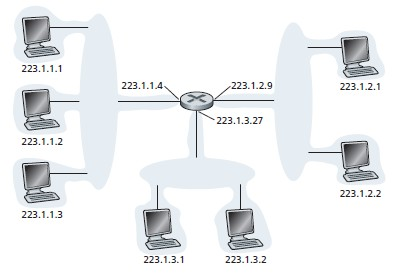
\includegraphics[width=0.5\linewidth]{cap14/3subnet.png}
\end{center}
Un router con tre interfacce collega sette host, divisi in tre subnet (sinistra, destra, sotto), ciascuna collegata a
un'interfaccia del router.
\begin{itemize}
    \item La subnet di sinistra ha indirizzo \texttt{223.1.1.0/24}: tutte le interfacce hanno indirizzi della forma
          \texttt{223.1.1.xxx} --- \texttt{223.1.1.1}, \texttt{223.1.1.2}, \texttt{223.1.1.3} (host) e \texttt{223.1.1.4} (router).
    \item Le altre due subnet sono \texttt{223.1.2.0/24} e \texttt{223.1.3.0/24}.
\end{itemize}
\end{esempio}

\begin{esempio}{Tre router e sei subnet}
\begin{center}
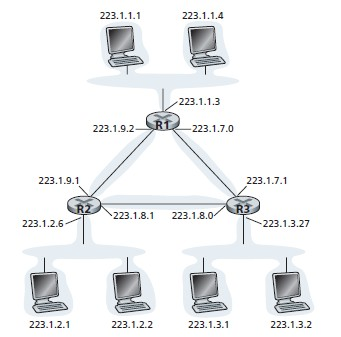
\includegraphics[width=0.42\linewidth]{cap14/6subnet.png}
\end{center}
Tre router sono collegati tra loro da collegamenti diretti punto-punto. Ogni router ha tre interfacce: una per ciascun
collegamento punto-punto e una per il collegamento broadcast verso una coppia di host. Le subnet sono \textbf{sei}:
\begin{itemize}
    \item \texttt{223.1.1.0/24} (R1--host), \texttt{223.1.2.0/24} (R2--host), \texttt{223.1.3.0/24} (R3--host);
    \item \texttt{223.1.9.0/24} (R1--R2), \texttt{223.1.8.0/24} (R2--R3), \texttt{223.1.7.0/24} (R3--R1).
\end{itemize}
Per contare le subnet si ``staccano'' le interfacce da host e router: ogni isola di rete che resta è una subnet, e anche un
collegamento punto-punto tra due router è una subnet. Le organizzazioni medio-grandi (aziende, università) hanno tipicamente
molte subnet interconnesse.
\end{esempio}

\begin{figure}[H]
\centering
\begin{tikzpicture}[every node/.style={font=\footnotesize\sffamily}]
  \node (pc) at (0,0) {\icon[1cm]{laptop}};
  \node[below=-2pt of pc, align=center] {host\\\texttt{192.168.1.4}\\maschera \texttt{255.255.255.0}};
  \node (r) at (5,0) {\icon[1.3cm]{accesspoint}};
  \node[below=-2pt of r, align=center] {router di casa (gateway)\\\texttt{192.168.1.1}};
  \node[netcloud, minimum width=2.4cm] (i) at (9.5,0) {Internet};
  \draw[wireless] (pc) -- (r); \draw[wired, line width=2pt] (r) -- (i);
  \node[draw, rounded corners, fill=cloudbg, text width=6cm, align=left, anchor=north] at (5,-1.8) {Per un indirizzo \textbf{nella stessa subnet} (192.168.1.x) l'host consegna direttamente; per \textbf{tutti gli altri} invia i pacchetti al \textbf{gateway}, cioè al router.};
\end{tikzpicture}
\caption{La configurazione tipica di un host di casa: indirizzo, maschera e gateway predefinito.}
\end{figure}

\subsection{ifconfig e ip}

Su Linux si può controllare il proprio indirizzo con \texttt{ifconfig} (\emph{interface configuration}; l'equivalente su
Windows è \texttt{ipconfig}), che elenca tutte le interfacce di rete della macchina con la loro configurazione
(indirizzi, maschere, \dots). Il comando moderno è \texttt{ip}.

\begin{lstlisting}[language=bash]
$ ifconfig          # configurazione di tutte le interfacce
$ ip addr           # lo stesso, con il comando moderno
\end{lstlisting}

% ══════════════════════════════════════════════════════════════
\section{L'indirizzamento su Internet}
% ══════════════════════════════════════════════════════════════

Dividere le grandi reti in reti più piccole è particolarmente importante su Internet, dove vanno collegati miliardi di
dispositivi (e ancora più interfacce). Gli indirizzi vanno assegnati con cura per evitare che:

\begin{itemize}
    \item le forwarding table dei router diventino enormi;
    \item interfacce diverse abbiano lo stesso indirizzo;
    \item si esauriscano gli indirizzi.
\end{itemize}

L'approccio è dare alle organizzazioni (ISP, aziende, enti) delle subnet, in due modi: l'indirizzamento
\textbf{classful} (vecchio, non più usato in pratica) e quello \textbf{classless} (attuale).

\subsection{Indirizzamento classful}

\begin{table}[H]
\centering
\begin{tabular}{llllr}
\toprule
\textbf{Classe} & \textbf{Formato} & \textbf{Primo byte} & \textbf{Esempio} & \textbf{Indirizzi per rete} \\
\midrule
A & a.b.c.d/8 & 0--127 & 10.X.X.X & oltre 16 milioni \\
B & a.b.c.d/16 & 128--191 & 150.10.X.X & 65\,536 \\
C & a.b.c.d/24 & 192--223 & 200.10.10.X & 256 (254 host) \\
\bottomrule
\end{tabular}
\caption{Le classi di indirizzi (le classi D, 224--239, ed E, 240--255, erano riservate a multicast e usi sperimentali).}
\end{table}

\begin{esempio}{Lo spreco del classful}
Un'organizzazione che ha bisogno di 300 indirizzi non può usare una classe C (troppo piccola): riceve una classe B, per
esempio \texttt{241.115.0.0/16}, con tutti i suoi 65\,536 indirizzi. Ne usa 300, e ne \textbf{spreca oltre 65\,000}.
\end{esempio}

\subsection{Indirizzamento classless (CIDR)}

\dfn{CIDR}{
    L'approccio moderno, più flessibile, si chiama \textbf{Classless InterDomain Routing} (CIDR, pronunciato come
    ``\emph{cider}''). A un'organizzazione si può assegnare un indirizzo di rete della forma \texttt{a.b.c.d/x}, con
    $x$ \textbf{qualsiasi}.
    \begin{itemize}
      \item La parte di rete dell'indirizzo si chiama \textbf{prefisso}.
      \item L'insieme di indirizzi riservati all'organizzazione si chiama \textbf{blocco}.
    \end{itemize}
}

\begin{esempio}{300 indirizzi con CIDR}
Servono 300 indirizzi: bastano 9 bit di host ($2^9 = 512 \geq 300$), quindi un prefisso di $32 - 9 = 23$ bit. L'organizzazione
riceve per esempio \texttt{241.115.2.0/23}: 512 indirizzi, con soli 212 sprecati (invece di oltre 65\,000).
\end{esempio}

\warning{Blocchi che si sovrappongono}{
    I blocchi possono sovrapporsi: in questo caso è la \textbf{lunghezza del prefisso} a distinguerli. Per esempio
    \texttt{10.10.10.15/16} \textbf{non} è nello stesso blocco di \texttt{10.10.10.14/24}: il primo appartiene a
    \texttt{10.10.0.0/16}, il secondo a \texttt{10.10.10.0/24}.
}

\subsection{Subnet interne a un blocco}

Dentro un blocco CIDR si possono creare \textbf{subnet interne} all'organizzazione. Il blocco \texttt{241.115.0.0/16}, per
esempio, si può dividere in:
\texttt{241.115.1.0/24} (subnet 1), \texttt{241.115.2.0/24} (subnet 2), \texttt{241.115.3.0/24} (subnet 3), e così via.

\begin{figure}[H]
\centering
\begin{tikzpicture}[every node/.style={font=\small\ttfamily}]
  \node[draw, fill=lnet!60, minimum width=4.4cm, minimum height=0.7cm] (p) at (0,0) {11110001 01110011};
  \node[draw, fill=ltra!60, minimum width=2.2cm, minimum height=0.7cm, right=0pt of p] (s) {SSSSSSSS};
  \node[draw, fill=lapp!60, minimum width=2.2cm, minimum height=0.7cm, right=0pt of s] (h) {HHHHHHHH};
  \draw[decorate, decoration={brace, amplitude=5pt}] (p.north west) -- (p.north east) node[midway, above=6pt, font=\footnotesize\sffamily] {prefisso dell'organizzazione (/16)};
  \draw[decorate, decoration={brace, amplitude=5pt}] (s.north west) -- (s.north east) node[midway, above=6pt, font=\footnotesize\sffamily] {subnet};
  \draw[decorate, decoration={brace, amplitude=5pt}] (h.north west) -- (h.north east) node[midway, above=6pt, font=\footnotesize\sffamily] {host};
\end{tikzpicture}
\caption{Un blocco /16 diviso internamente in subnet /24.}
\end{figure}

\begin{esempio}{Dividere un blocco in sottoblocchi uguali}
Un ISP ha il blocco \texttt{200.23.16.0/20} e vuole dividerlo tra 8 organizzazioni. Servono $\log_2 8 = 3$ bit in più: i
sottoblocchi sono /23, ciascuno da $2^9 = 512$ indirizzi. Il terzo byte vale $16 = \texttt{0001}\,\texttt{0000}$: i 4 bit
evidenziati sono del prefisso /20, i 3 successivi numerano l'organizzazione.
\begin{center}
\begin{tabular}{lll}
\toprule
\textbf{Organizzazione} & \textbf{Terzo byte} & \textbf{Blocco} \\
\midrule
0 & \texttt{0001 000}0 & 200.23.16.0/23 \\
1 & \texttt{0001 001}0 & 200.23.18.0/23 \\
2 & \texttt{0001 010}0 & 200.23.20.0/23 \\
\dots & \dots & \dots \\
7 & \texttt{0001 111}0 & 200.23.30.0/23 \\
\bottomrule
\end{tabular}
\end{center}
\end{esempio}

% ══════════════════════════════════════════════════════════════
\section{L'aggregazione degli indirizzi}
% ══════════════════════════════════════════════════════════════

L'indirizzamento basato sui prefissi è utilissimo ai dispositivi che collegano prefissi diversi: un router può
ricordare (cioè scrivere nella forwarding table) solo i \textbf{prefissi}. Quando riceve un messaggio con un certo
prefisso lo inoltra verso un router più specifico, e così via.

\dfn{Aggregazione degli indirizzi}{
    L'\textbf{aggregazione degli indirizzi} (\emph{address aggregation} o \emph{route summarization}) consiste
    nell'annunciare al resto della rete un \textbf{unico prefisso} che riassume molti blocchi più piccoli.
}

\begin{figure}[H]
\centering
\begin{tikzpicture}[every node/.style={font=\scriptsize\sffamily}, org/.style={draw, rounded corners, fill=cloudbg, minimum width=3.4cm, align=center}]
  \node[org] (o0) at (0,2.4) {Organizzazione 0\\\texttt{200.23.16.0/23}};
  \node[org] (o1) at (0,1.2) {Organizzazione 1\\\texttt{200.23.18.0/23}};
  \node[org] (o2) at (0,0) {Organizzazione 2\\\texttt{200.23.20.0/23}};
  \node at (0,-0.8) {$\vdots$};
  \node[org] (o7) at (0,-1.7) {Organizzazione 7\\\texttt{200.23.30.0/23}};
  \node (isp) at (5,0.5) {\icon[1.1cm]{router}}; \node[below=-2pt of isp] {ISP1};
  \node[netcloud, minimum width=2.4cm] (net) at (9.6,0.5) {Internet};
  \foreach \o in {o0,o1,o2,o7} \draw[thick] (\o.east) -- (isp);
  \draw[wired, line width=2pt] (isp) -- (net);
  \node[draw, fill=llink!60, rounded corners, text width=4cm, align=center] at (7.3,2.2) {``mandatemi tutto ciò che inizia con \texttt{200.23.16.0/20}''};
\end{tikzpicture}
\caption{ISP1 annuncia un solo prefisso /20 per le otto organizzazioni: il resto di Internet ha bisogno di una sola riga.}
\end{figure}

Che succede se l'Organizzazione 1 cambia fornitore e passa a ISP2, portandosi dietro il proprio blocco?

\begin{figure}[H]
\centering
\begin{tikzpicture}[every node/.style={font=\scriptsize\sffamily}, org/.style={draw, rounded corners, fill=cloudbg, minimum width=3.4cm, align=center}]
  \node[org] (o0) at (0,2.4) {Organizzazione 0\\\texttt{200.23.16.0/23}};
  \node[org] (o7) at (0,1.0) {Organizzazione 7\\\texttt{200.23.30.0/23}};
  \node[org, fill=netorange!20] (o1) at (0,-1.2) {Organizzazione 1\\\texttt{200.23.18.0/23}};
  \node (isp1) at (5,1.7) {\icon[1cm]{router}}; \node[below=-2pt of isp1] {ISP1};
  \node (isp2) at (5,-1.2) {\icon[1cm]{router}}; \node[below=-2pt of isp2] {ISP2};
  \node[netcloud, minimum width=2.4cm] (net) at (9.6,0.3) {Internet};
  \draw[thick] (o0.east) -- (isp1); \draw[thick] (o7.east) -- (isp1); \draw[thick, netorange] (o1.east) -- (isp2);
  \draw[wired, line width=2pt] (isp1) -- (net); \draw[wired, line width=2pt] (isp2) -- (net);
  \node[draw, fill=llink!60, rounded corners, text width=3.6cm, align=center] at (7.6,2.6) {``tutto ciò che inizia con \texttt{200.23.16.0/20}''};
  \node[draw, fill=netorange!20, rounded corners, text width=3.6cm, align=center] at (7.6,-2.0) {``\dots ma \texttt{200.23.18.0/23} mandatelo a me!''};
\end{tikzpicture}
\caption{ISP2 annuncia il prefisso più specifico: grazie alla longest prefix matching i pacchetti per l'Organizzazione 1 vanno a ISP2, tutti gli altri del /20 a ISP1.}
\end{figure}

\begin{itemize}
    \item Un indirizzo dell'Organizzazione 1 corrisponde sia al /20 di ISP1 sia al /23 di ISP2; per la \textbf{longest prefix
          matching} vince il /23: nessuna ambiguità.
    \item Blocchi e sottoblocchi possono quindi essere assegnati a linee diverse senza ambiguità, con grande flessibilità.
    \item L'aggregazione è tanto più efficace quanto più i blocchi restano \textbf{raggruppati} (clusterizzati): ogni
          eccezione è una riga in più nelle tabelle.
\end{itemize}

% ══════════════════════════════════════════════════════════════
\section{Come ottenere un blocco di indirizzi}
% ══════════════════════════════════════════════════════════════

Per ottenere un blocco di indirizzi per le subnet di un'organizzazione ci sono due strade:

\begin{enumerate}
    \item \textbf{Contattare un ISP}, che fornisce indirizzi presi da un blocco più grande che gli è già stato assegnato. Per
          esempio l'ISP può avere il blocco \texttt{200.23.16.0/20} e dividerlo in sottoblocchi di dimensione variabile
          secondo le proprie politiche.
    \item \textbf{Rivolgersi all'ICANN} (\emph{Internet Corporation for Assigned Names and Numbers}), l'autorità globale no-profit
          responsabile dello spazio degli indirizzi IP (assegna i blocchi agli ISP, tramite registri regionali). L'ICANN gestisce
          anche i root server DNS, assegna i nomi di dominio e risolve le controversie sui nomi.
\end{enumerate}

% ══════════════════════════════════════════════════════════════
\section{Il datagramma IPv4}
% ══════════════════════════════════════════════════════════════

Il pacchetto del livello di rete di Internet si chiama \textbf{datagramma} (come in UDP).

\begin{figure}[H]
\centering
\begin{tikzpicture}[every node/.style={font=\scriptsize\sffamily}, x=0.45cm, y=0.62cm]
  \node[field, fill=lnet!60, minimum width=1.8cm, minimum height=0.62cm, anchor=north west] at (0,0) {versione};
  \node[field, fill=lnet!60, minimum width=1.8cm, minimum height=0.62cm, anchor=north west] at (4,0) {lungh. header};
  \node[field, fill=lnet!40, minimum width=3.6cm, minimum height=0.62cm, anchor=north west] at (8,0) {tipo di servizio};
  \node[field, fill=lnet!40, minimum width=7.2cm, minimum height=0.62cm, anchor=north west] at (16,0) {lunghezza del datagramma (byte)};
  \node[field, fill=netorange!30, minimum width=7.2cm, minimum height=0.62cm, anchor=north west] at (0,-1) {identificatore (16)};
  \node[field, fill=netorange!30, minimum width=1.35cm, minimum height=0.62cm, anchor=north west] at (16,-1) {flag (3)};
  \node[field, fill=netorange!30, minimum width=5.85cm, minimum height=0.62cm, anchor=north west] at (19,-1) {offset del frammento (13)};
  \node[field, fill=netred!20, minimum width=3.6cm, minimum height=0.62cm, anchor=north west] at (0,-2) {time to live (8)};
  \node[field, fill=ltra!50, minimum width=3.6cm, minimum height=0.62cm, anchor=north west] at (8,-2) {protocollo superiore};
  \node[field, fill=lnet!40, minimum width=7.2cm, minimum height=0.62cm, anchor=north west] at (16,-2) {checksum dell'header (16)};
  \node[field, fill=llink!70, minimum width=14.4cm, minimum height=0.62cm, anchor=north west] at (0,-3) {indirizzo IP sorgente (32)};
  \node[field, fill=llink!70, minimum width=14.4cm, minimum height=0.62cm, anchor=north west] at (0,-4) {indirizzo IP destinazione (32)};
  \node[field, fill=lphy!60, minimum width=14.4cm, minimum height=0.62cm, anchor=north west] at (0,-5) {opzioni (se presenti)};
  \node[field, fill=cloudbg, minimum width=14.4cm, minimum height=1.2cm, anchor=north west] at (0,-6) {dati (tipicamente un segmento TCP o UDP)};
  \draw[{Stealth}-{Stealth}] (0,0.5) -- node[above] {32 bit} (32,0.5);
  \draw[decorate, decoration={brace, amplitude=5pt}] (32.4,0) -- (32.4,-5) node[midway, right=6pt, align=left] {header:\\20 byte\\senza opzioni};
\end{tikzpicture}
\caption{Il datagramma IPv4.}
\end{figure}

\begin{itemize}
    \item \textbf{Versione} (4 bit): la versione di IP (4 o 6); il formato dipende dalla versione.
    \item \textbf{Lunghezza dell'header} (4 bit): la dimensione dell'header, non fissa per via delle opzioni; serve a sapere
          dove iniziano i dati. Senza opzioni l'header è di \textbf{20 byte}.
    \item \textbf{Tipo di servizio} (TOS, 8 bit): proprietà specifiche del datagramma (per esempio tempo reale o no),
          definite dagli amministratori dei router.
    \item \textbf{Lunghezza del datagramma} (16 bit): lunghezza in byte di header + dati. I datagrammi raramente superano
          i 1500 byte, sui 65\,535 possibili.
    \item \textbf{Identificatore} (16 bit): numero progressivo che identifica il datagramma (usato nella frammentazione).
    \item \textbf{Flag e offset del frammento} (3 + 13 bit): proprietà e posizione del frammento (usati nella frammentazione).
    \item \textbf{Time-to-live} (TTL, 8 bit): impedisce che i datagrammi circolino per sempre. Ogni router che elabora il
          datagramma lo \textbf{decrementa di 1}; se arriva a 0, il router \textbf{scarta} il datagramma.
    \item \textbf{Protocollo superiore} (8 bit): il protocollo di trasporto a cui consegnare i dati (per esempio \textbf{6} per
          TCP, \textbf{17} per UDP; l'elenco completo è sul sito della IANA).
    \item \textbf{Checksum dell'header} (16 bit): complemento a 1 della somma a 16 bit dell'header. I router lo controllano e di
          solito scartano i datagrammi errati. Va \textbf{ricalcolato a ogni router}, perché TTL e opzioni possono cambiare.
    \item \textbf{Indirizzi IP sorgente e destinazione} (32 + 32 bit).
    \item \textbf{Opzioni} (lunghezza variabile): estendono l'header con funzionalità aggiuntive. Aggiungono complessità (la
          dimensione non è nota a priori) e in IPv6 non esistono più.
    \item \textbf{Dati} (lunghezza variabile): il payload, tipicamente un segmento TCP o UDP.
\end{itemize}

\info{Quanto pesano gli header}{
    Un segmento TCP dentro un datagramma IP porta almeno 40 byte di header (20 TCP + 20 IP), più l'header del
    livello applicativo. Per messaggi piccoli l'overhead è significativo.
}

% ══════════════════════════════════════════════════════════════
\section{La frammentazione IPv4}
% ══════════════════════════════════════════════════════════════

Il primo problema dei datagrammi IP è che possono dover essere \textbf{frammentati} a causa del livello di
collegamento: protocolli di collegamento diversi trasportano pacchetti di dimensioni diverse (i frame Ethernet, per
esempio, portano al massimo 1500 byte di dati).

\dfn{MTU}{
    I datagrammi IP vengono incapsulati in frame di collegamento per essere trasportati da un nodo all'altro. La
    quantità massima di dati che un frame può trasportare è la \textbf{Maximum Transmission Unit} (MTU). A livello di
    collegamento la lunghezza del frame è limitata dai vincoli della trasmissione fisica.
}

\begin{figure}[H]
    \centering
    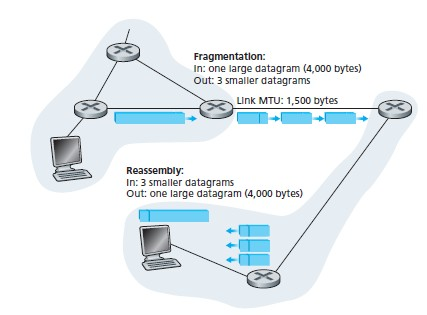
\includegraphics[width=0.55\linewidth]{cap14/frammentazione.png}
    \caption{Un router frammenta un datagramma da 4000 byte per un collegamento con MTU di 1500 byte; la destinazione riassembla i tre frammenti.}
\end{figure}

Un router che collega due collegamenti con MTU diverse può ricevere dal collegamento in ingresso un datagramma che non
entra in quello in uscita. Deve allora dividere il payload in due o più datagrammi più piccoli, i
\textbf{frammenti}, che vengono incapsulati in frame e inoltrati.

\subsection{Come funziona la frammentazione}

Quando un router frammenta un datagramma:

\begin{itemize}
    \item copia nei nuovi frammenti lo stesso \textbf{identificatore}, lo stesso indirizzo sorgente e lo stesso indirizzo di destinazione;
    \item imposta il campo \textbf{offset} di ciascun frammento con numeri progressivi (la posizione dei suoi dati nel
          datagramma originale, misurata in multipli di 8 byte);
    \item imposta il \textbf{flag} (``more fragments'') a 1 in tutti i frammenti tranne l'ultimo, dove vale 0: così si capisce
          che i frammenti sono finiti.
\end{itemize}

\begin{esempio}{4000 byte su un collegamento con MTU di 1500}
Un datagramma di 4000 byte (20 di header + 3980 di dati) con identificatore 777 deve attraversare un collegamento con MTU
di 1500 byte. Ogni frammento può portare al massimo $1500 - 20 = 1480$ byte di dati (multiplo di 8).
\begin{center}
\begin{tabular}{ccccc}
\toprule
\textbf{Frammento} & \textbf{Byte di dati} & \textbf{Identificatore} & \textbf{Offset} & \textbf{Flag} \\
\midrule
1 & 1480 (byte 0--1479) & 777 & $0/8 = 0$ & 1 \\
2 & 1480 (byte 1480--2959) & 777 & $1480/8 = 185$ & 1 \\
3 & 1020 (byte 2960--3979) & 777 & $2960/8 = 370$ & 0 \\
\bottomrule
\end{tabular}
\end{center}
Il terzo frammento è lungo $1020 + 20 = 1040$ byte in tutto. La somma dei dati è $1480 + 1480 + 1020 = 3980$ byte.
\end{esempio}

\warning{Il riassemblaggio avviene negli host}{
    I frammenti vanno riassemblati prima di arrivare al trasporto, perché TCP e UDP si aspettano segmenti completi. I
    progettisti di IPv4 ritennero che riassemblare nei router avrebbe complicato il protocollo e rallentato i router:
    in IPv4 il \textbf{riassemblaggio è eseguito dagli end system}.
    \begin{itemize}
      \item Se l'host riceve più datagrammi con gli stessi indirizzi e lo stesso identificatore, capisce che il datagramma
            originale è stato frammentato.
      \item Deve ricostruire il datagramma originale dai frammenti, usando offset e flag. Se un frammento si perde, si
            scarta l'intero datagramma.
    \end{itemize}
}

% ══════════════════════════════════════════════════════════════
\section{Riepilogo}
% ══════════════════════════════════════════════════════════════

\riepilogo{
\begin{itemize}
    \item Un indirizzo IPv4 è di 32 bit, scritto in notazione decimale puntata; appartiene a un'\textbf{interfaccia}.
    \item Indirizzo = \textbf{prefisso} (subnet) + parte di host; la \textbf{subnet mask} (o /x) dice quanti bit sono di prefisso.
          Due host sono nella stessa subnet se IP AND maschera coincide.
    \item Una subnet /x ha $2^{32-x}$ indirizzi e $2^{32-x}-2$ host.
    \item Dal \textbf{classful} (A, B, C, sprechi) al \textbf{CIDR} (a.b.c.d/x qualsiasi); \textbf{aggregazione} dei prefissi con
          longest prefix matching per le eccezioni.
    \item Header IPv4: 20 byte + opzioni; campi chiave TTL, protocollo, checksum, indirizzi, identificatore/flag/offset.
    \item \textbf{Frammentazione}: se il datagramma supera l'MTU, i router lo dividono; gli host lo riassemblano.
\end{itemize}
}
          % Indirizzamento IPv4
  \chapter{DHCP, NAT e IPv6}

% ══════════════════════════════════════════════════════════════
\section{L'assegnazione degli indirizzi IP}
% ══════════════════════════════════════════════════════════════

Dentro un blocco di indirizzi, gli indirizzi IP vanno assegnati alle singole interfacce. Un amministratore di sistema
può farlo in due modi:

\begin{itemize}
    \item \textbf{manualmente}: assegnando a mano un indirizzo a ciascun host (indirizzo \emph{statico});
    \item \textbf{automaticamente}: è la rete ad assegnare un indirizzo libero agli host che arrivano.
\end{itemize}

Il secondo approccio, il più comune, si realizza con il \textbf{Dynamic Host Configuration Protocol} (DHCP).

\dfn{DHCP}{
    Il \textbf{DHCP} assegna automaticamente a un host che si collega alla rete le informazioni necessarie per
    usarla: oltre all'\textbf{indirizzo IP}, la \textbf{subnet mask}, l'indirizzo del \textbf{gateway predefinito}
    (per uscire dalla rete) e quello del \textbf{server DNS locale}. È \emph{plug-and-play}, ed è quello che si usa
    nelle nostre case.
}

% ══════════════════════════════════════════════════════════════
\section{Il funzionamento del DHCP}
% ══════════════════════════════════════════════════════════════

Il DHCP è un protocollo \textbf{client-server}: un host appena arrivato (client) contatta il server DHCP per ricevere
la configurazione di rete. Il servizio può essere offerto da un computer o dal router stesso. Formalmente, il DHCP è un
protocollo di \textbf{livello applicativo} (usa UDP).

Riprendiamo l'esempio delle tre subnet collegate da un router, e supponiamo che la subnet di destra
(\texttt{223.1.2.0/24}) abbia un server DHCP: quando un nuovo host entra nella rete, ``contratta'' il proprio indirizzo
con il server. L'aggiunta di un host avviene in quattro passi (ricordati spesso con l'acronimo \textbf{DORA}):

\begin{figure}[H]
\centering
\begin{minipage}{0.34\linewidth}\centering
  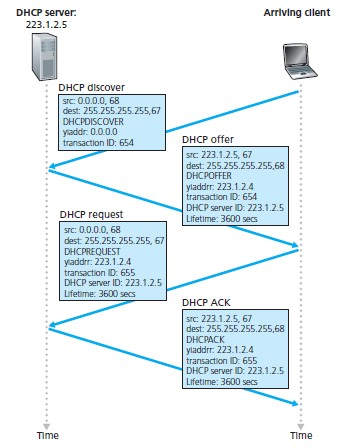
\includegraphics[width=0.9\linewidth]{cap15/dhcp_messaggi.png}
\end{minipage}\hfill
\begin{minipage}{0.62\linewidth}
\begin{enumerate}
  \item \textbf{Discover} --- ricerca del server: il nuovo host invia in \textbf{broadcast} un messaggio \emph{DHCP discover}
        (UDP, porta \textbf{67}) per trovare un server DHCP.
        \begin{itemize}
          \item IP destinazione: \texttt{255.255.255.255} (broadcast);
          \item IP sorgente: \texttt{0.0.0.0} (``questo host'', che non ha ancora un indirizzo);
          \item un identificativo di transazione casuale.
        \end{itemize}
  \item \textbf{Offer} --- offerta: poiché possono esserci più server, ogni server che riceve il discover risponde con un
        messaggio in broadcast (porta \textbf{68}) che offre una possibile configurazione (campo \texttt{yiaddr}, \emph{Your
        Internet ADDRess}). IP destinazione \texttt{255.255.255.255}, IP sorgente quello del server (\texttt{223.1.2.5}).
  \item \textbf{Request} --- richiesta: il client sceglie un'offerta tra quelle ricevute e la accetta ``facendo l'eco''
        del messaggio di offerta.
  \item \textbf{ACK} --- conferma: il server conferma la transazione con un messaggio finale.
\end{enumerate}
\end{minipage}
\caption{I quattro messaggi del DHCP (da Kurose).}
\end{figure}

\warning{Perché tutto in broadcast}{
    Nel passo 1 il client \textbf{non ha ancora un indirizzo} e \textbf{non sa dove sia il server}: l'unico modo di
    raggiungerlo è il broadcast. Anche l'offerta viaggia in broadcast, perché il client non può ancora ricevere
    pacchetti indirizzati a un IP che non ha. L'indirizzo assegnato ha una \textbf{durata} (\emph{lease time}): scaduta,
    va rinnovata, altrimenti può essere riassegnata a un altro host.
}

\subsection{Il DHCP relay agent}

\begin{itemize}
    \item Nell'esempio tutto funziona perché il server DHCP e l'host sono nella \textbf{stessa subnet}: i broadcast non
          attraversano i router.
    \item Se il server esiste ma sta in un'altra subnet, serve un \textbf{DHCP relay agent} che inoltri i messaggi DHCP (può
          farlo un router).
    \item Configurando il router come relay agent, anche gli host delle subnet \texttt{223.1.1.0/24} e \texttt{223.1.3.0/24}
          vengono serviti dal server DHCP della subnet \texttt{223.1.2.0/24}.
\end{itemize}

\subsection{Verificare la configurazione}

Su Linux il comando \texttt{ip} mostra la configurazione ricevuta dal DHCP:

\begin{lstlisting}[language=bash]
$ ip addr       # indirizzo IP e maschera delle interfacce
$ ip route      # gateway predefinito (riga "default via ...")
\end{lstlisting}

% ══════════════════════════════════════════════════════════════
\section{Il problema della visibilità}
% ══════════════════════════════════════════════════════════════

Su Internet ci sono miliardi di dispositivi che dovrebbero avere un indirizzo IP univoco per essere raggiungibili da
chiunque. Ma è davvero necessario che \textbf{tutti} i dispositivi siano visibili a tutti? È una buona idea che la mia
stampante sia raggiungibile (e usabile) da chiunque su Internet?

Avere tutti i dispositivi raggiungibili dall'esterno delle reti locali pone problemi evidenti:

\begin{itemize}
    \item gli indirizzi IP sono \textbf{finiti} (e gli IPv4 praticamente esauriti);
    \item se i dispositivi sono collegati localmente, spesso è irragionevole o indesiderabile esporli tutti su Internet;
    \item gli amministratori locali dovrebbero conoscere la struttura dei blocchi di indirizzi soprastanti per assegnare
          indirizzi liberi, cosa che spesso non dipende da loro (per esempio nelle reti di casa).
\end{itemize}

% ══════════════════════════════════════════════════════════════
\section{Il NAT}
% ══════════════════════════════════════════════════════════════

\dfn{Network Address Translation (NAT)}{
    Il servizio di \textbf{NAT} permette di \textbf{rimappare} gli indirizzi IP dei pacchetti di una rete in indirizzi
    diversi (\emph{network masquerading}). Si usa una \textbf{tabella di traduzione} che associa molte coppie
    indirizzo/porta locali (della LAN) a una coppia indirizzo/porta globale (della WAN). Il servizio può essere offerto
    dai router.
}

La rete locale mascherata si chiama \textbf{rete privata} (o \emph{realm} con indirizzi privati): gli indirizzi privati
sono validi \textbf{solo all'interno} della rete privata.

\begin{figure}[H]
\centering
\begin{tikzpicture}[every node/.style={font=\footnotesize\sffamily}]
  \node (pc) at (0,1.4) {\icon[0.9cm]{pc}}; \node[left=0pt of pc, font=\scriptsize\ttfamily] {192.168.0.23};
  \node (lp) at (0,0) {\icon[1cm]{laptop}}; \node[left=0pt of lp, font=\scriptsize\ttfamily] {192.168.0.11};
  \node (ph) at (0,-1.4) {\icon[0.6cm]{smartphone}}; \node[left=0pt of ph, font=\scriptsize\ttfamily] {192.168.0.7};
  \node (r) at (4,0) {\icon[1.3cm]{router}}; \node[below=0pt of r, align=center] {router NAT};
  \foreach \n in {pc,lp,ph} \draw[wired] (\n) -- (r);
  \node[netcloud, minimum width=3cm] (i) at (9,0) {Internet};
  \draw[wired, line width=2pt] (r) -- node[above, font=\scriptsize\ttfamily] {203.0.113.221} (i);
  \draw[decorate, decoration={brace, amplitude=6pt, mirror}] (-1.8,-2.1) -- (4.6,-2.1) node[midway, below=7pt, text=netgreen!50!black] {rete privata: indirizzi 192.168.0.x};
  \draw[decorate, decoration={brace, amplitude=6pt, mirror}] (4.8,-2.1) -- (10.6,-2.1) node[midway, below=7pt, text=netblue] {per Internet c'è un solo indirizzo pubblico};
\end{tikzpicture}
\caption{Con il NAT tutti i dispositivi di casa escono verso Internet con lo stesso indirizzo pubblico del router.}
\end{figure}

\subsection{Un esempio di NAT}

\begin{figure}[H]
    \centering
    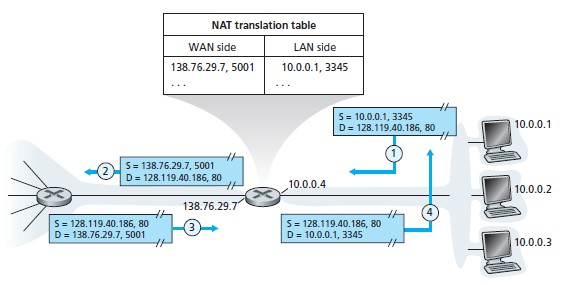
\includegraphics[width=0.7\linewidth]{cap15/nat_esempio.png}
    \caption{Un router NAT tra una rete privata 10.0.0.0/24 e Internet (da Kurose).}
\end{figure}

Le quattro interfacce della rete locale hanno indirizzi della subnet \texttt{10.0.0.0/24}; lato Internet il router ha un solo
indirizzo, \texttt{138.76.29.7}. Il router si comporta da ``passamessaggi'' che sovrascrive gli indirizzi secondo la tabella:

\begin{enumerate}
    \item L'host \texttt{10.0.0.1} invia un datagramma verso il server Web \texttt{128.119.40.186}, porta 80, usando la porta sorgente 3345.
    \item Il router NAT riceve il datagramma, sceglie una porta libera (\textbf{5001}), \textbf{sostituisce} indirizzo e porta sorgente
          con \texttt{138.76.29.7, 5001} e aggiunge la riga alla tabella di traduzione.
    \item Il server risponde a \texttt{138.76.29.7, 5001}: per lui, la richiesta è arrivata dal router.
    \item Il router riceve la risposta, cerca \texttt{138.76.29.7, 5001} nella tabella e \textbf{riscrive} destinazione e porta con
          \texttt{10.0.0.1, 3345}, poi la inoltra nella LAN.
\end{enumerate}

\begin{table}[H]
\centering
\begin{tabular}{ll}
\toprule
\textbf{Lato WAN} & \textbf{Lato LAN} \\
\midrule
138.76.29.7, 5001 & 10.0.0.1, 3345 \\
138.76.29.7, 5002 & 10.0.0.2, 3345 \\
\dots & \dots \\
\bottomrule
\end{tabular}
\caption{La tabella di traduzione NAT: la seconda riga mostra perché serve una porta nuova.}
\end{table}

\warning{Perché il NAT cambia anche la porta}{
    Gli host non sanno nulla del traffico degli altri host: due host della LAN potrebbero scegliere \textbf{la stessa
    porta} sorgente (3345) nello stesso momento. Il NAT non può quindi riusare la porta iniziale, e ne assegna una nuova.
    Poiché la porta è di 16 bit, un NAT può gestire \textbf{oltre 60\,000 connessioni} contemporanee con un solo indirizzo IP pubblico.
}

\subsection{Il limite del NAT}

\info{NAT traversal}{
    Nell'esempio la comunicazione è stata \textbf{iniziata dall'host interno} \texttt{10.0.0.1}: la riga della tabella nasce
    proprio da quel primo pacchetto in uscita. Se un pacchetto arriva da Internet \textbf{senza comunicazioni precedenti}
    (qualcuno vuole contattare un server che sta dietro il NAT), il router non ha informazioni sufficienti per sapere a quale
    host interno consegnarlo. Servono allora tecniche aggiuntive, dette di \textbf{NAT traversal} (per esempio l'inoltro
    manuale delle porte sul router, o protocolli per scoprire e aprire le mappature). Il NAT è anche criticato perché un router,
    dispositivo di livello 3, modifica i numeri di porta, che appartengono al livello 4.
}

% ══════════════════════════════════════════════════════════════
\section{Gli indirizzi IP riservati}
% ══════════════════════════════════════════════════════════════

Perché gli amministratori locali possano organizzare una rete privata senza interferenze, per convenzione alcuni blocchi di
indirizzi sono \textbf{riservati}: ISP e ICANN non possono assegnarli a nessuna organizzazione.

\begin{table}[H]
\centering
\begin{tabular}{llp{7.5cm}}
\toprule
\textbf{Blocco} & \textbf{Intervallo} & \textbf{Uso} \\
\midrule
10.0.0.0/8 & 10.0.0.0 -- 10.255.255.255 & reti private \\
172.16.0.0/12 & 172.16.0.0 -- 172.31.255.255 & reti private \\
192.168.0.0/16 & 192.168.0.0 -- 192.168.255.255 & reti private (tipiche delle case) \\
127.0.0.0/8 & 127.0.0.0 -- 127.255.255.255 & ``questa macchina'' (\emph{loopback}), di solito 127.0.0.1 \\
0.0.0.0 & --- & rete corrente; per estensione, un indirizzo con la parte di host a 0 indica la rete \\
255.255.255.255 & --- & broadcast; per estensione, un indirizzo con la parte di host tutta a 1 è il broadcast della subnet \\
\bottomrule
\end{tabular}
\caption{Indirizzi IPv4 riservati.}
\end{table}

La riserva è necessaria perché gli indirizzi privati potrebbero coincidere con indirizzi pubblici, rendendo ambiguo
l'instradamento dentro la rete. Con blocchi riservati, un router sa che \texttt{192.168.x.x} non è mai un indirizzo di Internet.

% ══════════════════════════════════════════════════════════════
\section{ping e nmap per la scoperta degli host}
% ══════════════════════════════════════════════════════════════

Per verificare se un host è raggiungibile si usa \textbf{ping} (identico su Linux e Windows), basato su \textbf{ICMP}
(\emph{Internet Control Message Protocol}): invia all'host un pacchetto \emph{echo request} a cui l'host risponde
automaticamente con un \emph{echo reply}, e misura il tempo trascorso, cioè l'\textbf{RTT}. Lo vedremo in dettaglio nel
prossimo capitolo.

Oltre alla scansione delle porte, \textbf{nmap} può mappare i dispositivi di una rete, usando ping (ICMP) per scoprire gli host:

\begin{lstlisting}[language=bash]
$ ping [indirizzo]                               # l'host risponde?
$ sudo nmap -sn [indirizzo gateway]/[bit di subnet]  # quali host sono accesi nella subnet?
\end{lstlisting}

% ══════════════════════════════════════════════════════════════
\section{Esempio completo: configurare una LAN}
% ══════════════════════════════════════════════════════════════

Vogliamo creare una nuova rete locale (LAN) dentro una rete più grande preesistente (WAN). L'amministratore della WAN
ci fornisce:

\begin{itemize}
    \item l'indirizzo della WAN: \texttt{150.100.0.0/16};
    \item l'indirizzo del gateway che porta all'esterno (WAN/Internet): \texttt{150.100.50.1};
    \item un indirizzo libero per la nostra rete: \texttt{150.100.50.10}.
\end{itemize}

Useremo un router con NAT e decidiamo che la nuova LAN avrà indirizzo \texttt{192.168.1.0/24} (riservato alle reti private).

\begin{figure}[H]
\centering
\begin{tikzpicture}[every node/.style={font=\footnotesize\sffamily}]
  \node[netcloud, minimum width=2.8cm] (inet) at (0,3.2) {Internet};
  \node[draw=netblue, thick, rounded corners, fill=cloudbg, minimum width=7cm, minimum height=2.2cm] (wan) at (0,0.8) {};
  \node[anchor=north east, text=netblue] at (wan.north east) {WAN \texttt{150.100.0.0/16}};
  \node (rw) at (-1.8,1.0) {\icon[1.1cm]{router}}; \node[below=-1pt of rw, align=center, font=\scriptsize\sffamily] {router WAN\\\texttt{150.100.50.1}};
  \draw[wired, line width=2pt] (inet) -- (rw);
  \node[draw=netgreen!70!black, thick, rounded corners, fill=netgreen!8, minimum width=7cm, minimum height=2.6cm] (lan) at (0,-2.4) {};
  \node[anchor=south east, text=netgreen!50!black] at (lan.south east) {LAN \texttt{192.168.1.0/24}};
  \node (rl) at (-1.8,-1.6) {\icon[1.1cm]{router}};
  \node[anchor=west, font=\scriptsize\ttfamily, text=netblue] at (-1.2,-0.9) {WAN: 150.100.50.10};
  \node[anchor=west, font=\scriptsize\ttfamily, text=netgreen!50!black] at (-1.2,-1.8) {LAN: 192.168.1.1};
  \draw[wired] (rw) -- (rl);
  \node (h1) at (-2.3,-3.2) {\icon[0.8cm]{laptop}}; \node[right=0pt of h1, font=\scriptsize\ttfamily, align=left] {192.168.1.100\\(DHCP)};
  \node (h2) at (1.2,-3.2) {\icon[0.8cm]{pc}}; \node[right=0pt of h2, font=\scriptsize\ttfamily, align=left] {192.168.1.10\\(manuale)};
  \draw[wired] (rl) -- (h1); \draw[wired] (rl) -- (h2);
\end{tikzpicture}
\caption{La LAN da configurare: il router locale ha un'interfaccia nella WAN e una nella LAN.}
\end{figure}

\subsection{1. Il lato WAN del router}

Il router locale ha \textbf{due interfacce}, una verso la WAN e una verso la LAN. Sul lato WAN vanno impostati:

\begin{itemize}
    \item l'indirizzo del router nella WAN: \texttt{150.100.50.10};
    \item la subnet mask della WAN: \texttt{255.255.0.0};
    \item il gateway: \texttt{150.100.50.1};
    \item uno o più server DNS.
\end{itemize}

Se la WAN ha un servizio DHCP, si può anche scegliere un indirizzo dinamico.

\begin{figure}[H]
    \centering
    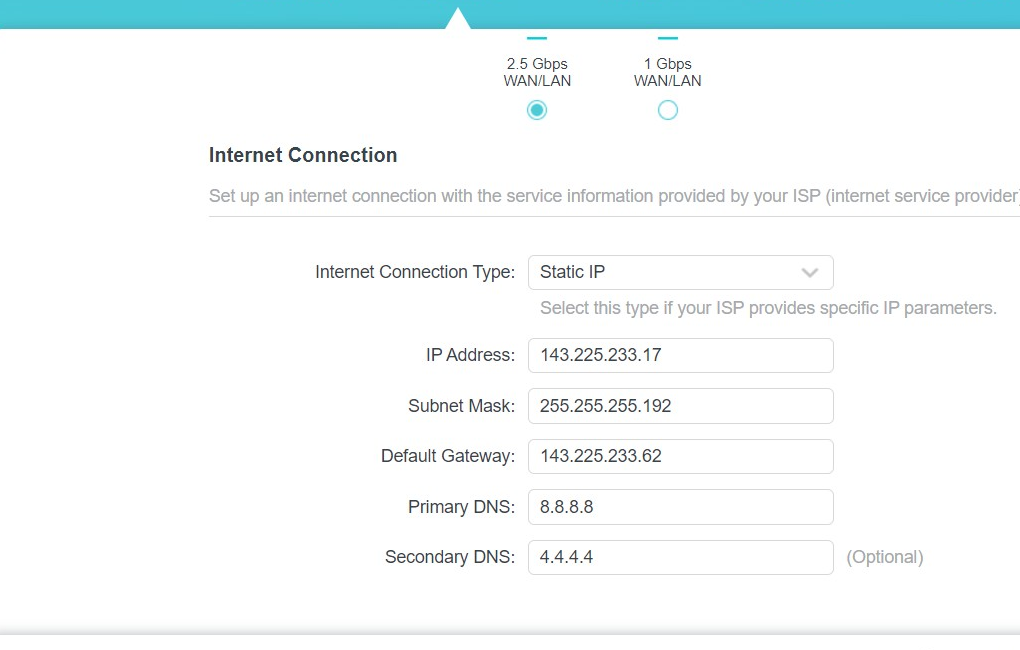
\includegraphics[width=0.6\linewidth]{cap15/config_wan.png}
    \caption{La pagina di configurazione ``Internet'' (lato WAN) di un router domestico: indirizzo statico, maschera, gateway e DNS (valori di un esempio reale, diversi da quelli del testo).}
\end{figure}

\subsection{2. Il lato LAN del router}

\begin{itemize}
    \item All'interfaccia LAN del router si dà un indirizzo della nuova rete: poiché la LAN è \texttt{192.168.1.0/24}, al router si
          assegna \texttt{192.168.1.1/24} (è consuetudine dare al router l'indirizzo \texttt{.1}).
    \item Se il router offre anche il DHCP, si specificano:
    \begin{itemize}
      \item il \textbf{pool di indirizzi} per gli host DHCP, per esempio da \texttt{192.168.1.100} a \texttt{192.168.1.250};
      \item il \textbf{lease time}: la durata dell'assegnazione, dopo la quale l'indirizzo può essere riusato;
      \item gateway e DNS da comunicare agli host.
    \end{itemize}
\end{itemize}

\begin{figure}[H]
    \centering
    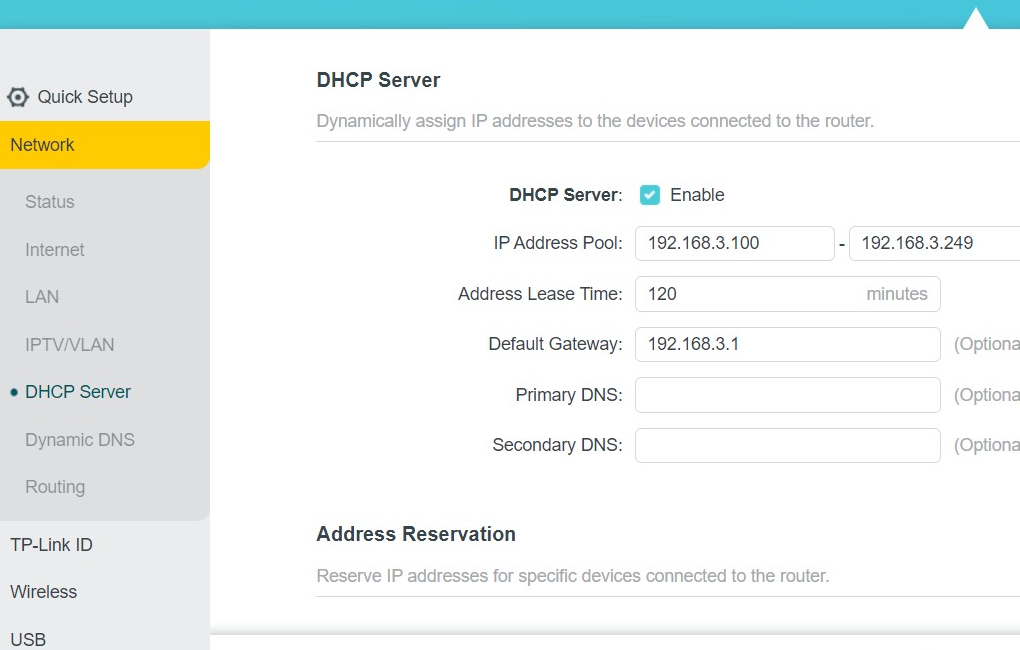
\includegraphics[width=0.6\linewidth]{cap15/config_lan.png}
    \caption{La configurazione del server DHCP del router: pool di indirizzi, lease time, gateway e DNS.}
\end{figure}

\subsection{3. Gli host}

Su un nuovo host (per esempio con Linux Mint) si può scegliere come configurare la connessione:

\begin{figure}[H]
\centering
\begin{minipage}{0.44\linewidth}\centering
  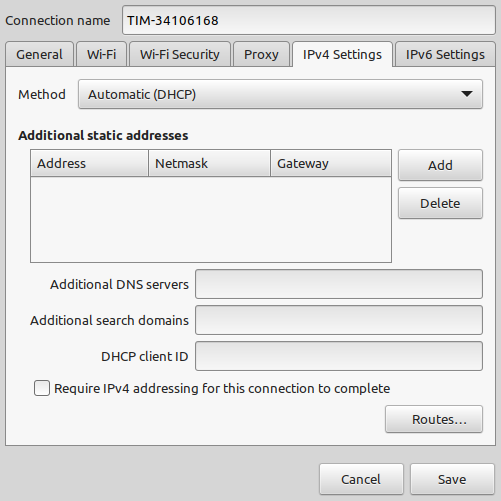
\includegraphics[width=0.85\linewidth]{cap15/host_dhcp.png}\\{\small (a) automatica (DHCP)}
\end{minipage}\hfill
\begin{minipage}{0.44\linewidth}\centering
  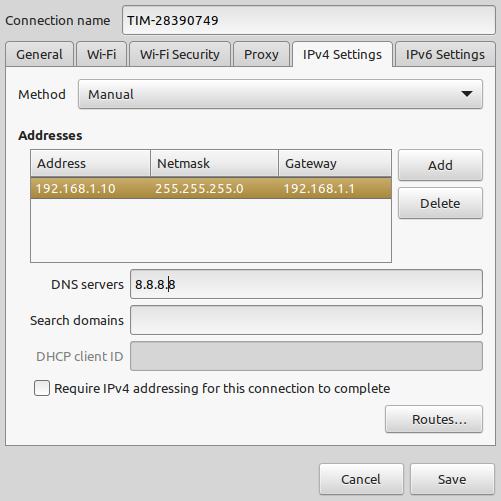
\includegraphics[width=0.85\linewidth]{cap15/host_manuale.png}\\{\small (b) manuale}
\end{minipage}
\caption{Configurazione della connessione su un host.}
\end{figure}

\begin{itemize}
    \item \textbf{Automatica (DHCP)}: l'host riceve dal DHCP un indirizzo tra \texttt{192.168.1.100} e \texttt{192.168.1.250}.
    \item \textbf{Manuale}: bisogna conoscere la configurazione della rete e gli indirizzi disponibili, e indicare
          l'\textbf{indirizzo dell'host} (statico, \textbf{fuori dal pool} del DHCP, per esempio \texttt{192.168.1.10}), la
          \textbf{subnet mask}, il \textbf{gateway} e uno o più \textbf{DNS}.
\end{itemize}

Gli host collegati inviano i loro pacchetti al router locale, senza sapere nulla della WAN esterna; il router locale è
configurato per inoltrarli al router della WAN, e da lì eventualmente a Internet.

\warning{Indirizzi manuali fuori dal pool}{
    Un indirizzo assegnato a mano deve stare \textbf{fuori} dall'intervallo del DHCP: altrimenti prima o poi il DHCP lo
    assegnerà anche a un altro host, e due interfacce avranno lo stesso indirizzo (conflitto).
}

% ══════════════════════════════════════════════════════════════
\section{IPv6}
% ══════════════════════════════════════════════════════════════

All'inizio degli anni '90 l'IETF (organizzazione nata nel 1986) avviò lo sviluppo di un successore di IPv4, per
affrontare la \textbf{carenza di indirizzi} a 32 bit. IPv6 fu progettato per avere molti più indirizzi, ma fu anche
l'occasione per aggiornare altri aspetti di IPv4 sulla base dell'esperienza accumulata.

\info{E IPv5?}{
    Non si sa esattamente quando gli IPv4 si esauriranno del tutto (si era ipotizzato il 2008, poi il 2018, e qualche
    indirizzo è ancora disponibile). \textbf{IPv5} fu proposto nel 1979 e si basava sullo sperimentale \emph{Internet Stream
    Protocol} (ST); usava ancora indirizzi a 32 bit, e fu abbandonato soprattutto per la stessa carenza di indirizzi.
}

\subsection{I vantaggi di IPv6}

\begin{itemize}
    \item \textbf{Indirizzi molto più grandi}: da 32 a \textbf{128 bit}, cioè $2^{128} \approx 3{,}4\cdot 10^{38}$ indirizzi. Il mondo
          non resterà senza indirizzi: si potrebbe dare un indirizzo a ogni granello di sabbia del pianeta.
    \item \textbf{Header di lunghezza fissa}, 40 byte: alcuni campi di IPv4 sono stati eliminati o resi facoltativi, e i router
          elaborano i pacchetti più velocemente.
    \item \textbf{Etichettatura dei flussi} (\emph{flow labeling}): i pacchetti di certe applicazioni (per esempio lo streaming
          audio/video) possono essere raggruppati in un flusso con un identificativo. Il ruolo preciso dei flussi è ancora discusso.
\end{itemize}

\info{Come si scrive un indirizzo IPv6}{
    Un indirizzo IPv6 si scrive come 8 gruppi di 4 cifre esadecimali separati da due punti, per esempio
    \texttt{2001:0db8:0000:0000:0000:ff00:0042:8329}. Gli zeri iniziali di ogni gruppo si possono omettere, e una sequenza di
    gruppi tutti a zero si può sostituire (una sola volta) con \texttt{::}: l'indirizzo diventa \texttt{2001:db8::ff00:42:8329}.
    L'indirizzo di loopback è \texttt{::1}.
}

\subsection{Il datagramma IPv6}

\begin{figure}[H]
    \centering
    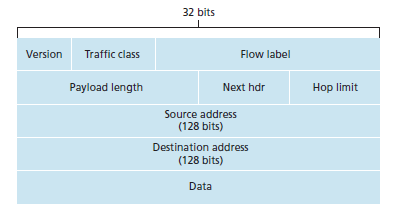
\includegraphics[width=0.55\linewidth]{cap15/ipv6_datagramma.png}
    \caption{Il datagramma IPv6: header fisso di 40 byte.}
\end{figure}

\begin{itemize}
    \item \textbf{Version} (4 bit): la versione, cioè 6.
    \item \textbf{Traffic class} (8 bit): come il TOS di IPv4, serve a dare priorità ai datagrammi (per esempio voce su IP rispetto a SMTP).
    \item \textbf{Flow label} (20 bit): identifica un flusso di datagrammi.
    \item \textbf{Payload length} (16 bit): numero di byte del payload (esclusi i 40 byte di header).
    \item \textbf{Next header} (8 bit): il protocollo superiore a cui consegnare i dati (TCP, UDP, \dots), come il campo protocollo di IPv4.
    \item \textbf{Hop limit} (8 bit): il time-to-live, decrementato a ogni inoltro.
    \item \textbf{Indirizzi sorgente e destinazione} (128 + 128 bit).
    \item \textbf{Data}: il payload.
\end{itemize}

\subsection{Cosa manca rispetto a IPv4}

\begin{itemize}
    \item \textbf{Campi della frammentazione}: IPv6 non permette frammentazione e riassemblaggio nei router intermedi, ma solo negli
          host. Se un router riceve un datagramma IPv6 troppo grande da inoltrare, lo \textbf{scarta} e rimanda al mittente un
          messaggio di errore ``\emph{Packet Too Big}''; il mittente rinvia i dati con datagrammi più piccoli.
    \item \textbf{Checksum dell'header}: richiede tempo in ogni router ed è ridondante, perché i protocolli di collegamento di
          solito controllano già l'intero pacchetto (e TCP/UDP controllano i propri dati).
    \item \textbf{Opzioni}: non fanno più parte dell'header standard; alcune si possono indicare nel campo \emph{next header}
          (accanto agli identificativi di TCP/UDP), come header di estensione.
\end{itemize}

% ══════════════════════════════════════════════════════════════
\section{Dalla IPv4 alla IPv6}
% ══════════════════════════════════════════════════════════════

C'è un grosso problema: IPv6 \textbf{non è retrocompatibile}. I sistemi che capiscono solo IPv4 non sanno gestire i datagrammi IPv6.
Come può Internet adottare IPv6?

\begin{itemize}
    \item \textbf{Flag day}: a una certa data e ora tutte le macchine di Internet vengono spente e aggiornate da IPv4 a IPv6. Un
          approccio simile fu usato quando fu introdotto TCP, e fu un disastro anche nella piccola Internet di allora: con miliardi
          di dispositivi è impensabile.
    \item \textbf{Tunneling}: router specifici (i \emph{tunnel}) incapsulano i datagrammi IPv6 dentro datagrammi IPv4 (e viceversa)
          in modo quasi trasparente, per attraversare le parti di rete che parlano solo IPv4. È l'approccio più realistico, già
          usato nella pratica.
\end{itemize}

\begin{figure}[H]
\centering
\begin{tikzpicture}[every node/.style={font=\scriptsize\sffamily}]
  \foreach \x/\n/\c in {0/A/lnet, 2.6/B/lnet, 5.2/C/lphy, 7.8/D/lphy, 10.4/E/lnet, 13/F/lnet} {
    \node (\n) at (\x,0) {\icon[0.9cm]{router}}; \node[above=-2pt of \n] {\n};
  }
  \node[below=0pt of A] {IPv6}; \node[below=0pt of B] {IPv6/v4}; \node[below=0pt of C] {IPv4}; \node[below=0pt of D] {IPv4}; \node[below=0pt of E] {IPv6/v4}; \node[below=0pt of F] {IPv6};
  \foreach \a/\b in {A/B, B/C, C/D, D/E, E/F} \draw[wired] (\a) -- (\b);
  \draw[very thick, netorange, rounded corners, dashed] (2.4,-1.2) rectangle (10.6,0.9);
  \node[text=netorange, font=\footnotesize\bfseries\sffamily] at (6.5,1.1) {tunnel};
  \node[field, fill=lnet!60, minimum width=1.6cm] at (1.3,-1.8) {datagramma IPv6};
  \node[field, fill=lphy!80, minimum width=1.1cm] (h4) at (5.6,-1.8) {header IPv4};
  \node[field, fill=lnet!60, minimum width=1.6cm, right=0pt of h4] {datagramma IPv6};
  \node[field, fill=lnet!60, minimum width=1.6cm] at (11.7,-1.8) {datagramma IPv6};
\end{tikzpicture}
\caption{Tunneling: B incapsula il datagramma IPv6 in un datagramma IPv4 per attraversare C e D; E lo estrae.}
\end{figure}

L'adozione di IPv6, inizialmente lenta, sta accelerando.

% ══════════════════════════════════════════════════════════════
\section{Riepilogo}
% ══════════════════════════════════════════════════════════════

\riepilogo{
\begin{itemize}
    \item Il \textbf{DHCP} assegna automaticamente indirizzo, maschera, gateway e DNS con quattro messaggi: discover, offer,
          request, ACK (broadcast, porte UDP 67/68); oltre le subnet serve un relay agent.
    \item Il \textbf{NAT} fa uscire una rete privata con un solo indirizzo pubblico, riscrivendo indirizzi e porte secondo una
          tabella; le connessioni avviate dall'esterno richiedono NAT traversal.
    \item Blocchi \textbf{riservati}: 10/8, 172.16/12, 192.168/16 (privati), 127/8 (loopback), 0.0.0.0, 255.255.255.255.
    \item \textbf{IPv6}: indirizzi a 128 bit, header fisso di 40 byte, flow label; niente frammentazione nei router, niente checksum,
          niente opzioni nell'header; transizione con \textbf{tunneling}.
\end{itemize}
}
          % DHCP, NAT, IPv6
  \chapter{ICMP, ping e traceroute}

% ══════════════════════════════════════════════════════════════
\section{Il protocollo ICMP}
% ══════════════════════════════════════════════════════════════

\dfn{ICMP}{
    L'\textbf{Internet Control Message Protocol} (ICMP) è un protocollo diagnostico e di controllo usato da host e
    router per scambiarsi informazioni sul livello di rete: segnalazioni di errore (destinazione irraggiungibile,
    TTL scaduto) e richieste di verifica (\emph{echo}). I messaggi ICMP viaggiano come \textbf{payload di datagrammi
    IP} (campo protocollo = 1), ma ICMP è considerato parte del livello di rete.
}

\begin{figure}[H]
\centering
\begin{tikzpicture}[every node/.style={font=\scriptsize\sffamily}]
  \node[field, fill=lnet, minimum width=2.4cm] (ip) at (0,0) {header IP (protocollo = 1)};
  \node[field, fill=netred!25, minimum width=1cm, right=0pt of ip] (ty) {tipo};
  \node[field, fill=netred!25, minimum width=1cm, right=0pt of ty] (co) {codice};
  \node[field, fill=netred!25, minimum width=1.4cm, right=0pt of co] (ck) {checksum};
  \node[field, fill=netred!10, minimum width=5.2cm, right=0pt of ck] {resto del messaggio (dipende dal tipo)};
  \draw[decorate, decoration={brace, amplitude=5pt}] ([yshift=2pt]ty.north west) -- ([yshift=2pt]12.2,0.33) node[midway, above=6pt] {messaggio ICMP, payload del datagramma IP};
\end{tikzpicture}
\caption{Un messaggio ICMP dentro un datagramma IP.}
\end{figure}

\begin{table}[H]
\centering
\begin{tabular}{ccl}
\toprule
\textbf{Tipo} & \textbf{Codice} & \textbf{Significato} \\
\midrule
0 & 0 & echo reply (risposta a ping) \\
3 & 0 & destinazione irraggiungibile: rete irraggiungibile \\
3 & 1 & destinazione irraggiungibile: host irraggiungibile \\
3 & 3 & destinazione irraggiungibile: \textbf{porta} irraggiungibile \\
3 & 4 & frammentazione necessaria ma vietata (``packet too big'') \\
8 & 0 & echo request (richiesta di ping) \\
11 & 0 & \textbf{TTL scaduto} (\emph{time exceeded}) \\
12 & 0 & header IP errato \\
\bottomrule
\end{tabular}
\caption{Alcuni tipi di messaggi ICMP.}
\end{table}

% ══════════════════════════════════════════════════════════════
\section{ping}
% ══════════════════════════════════════════════════════════════

ICMP è un protocollo con cui, sostanzialmente, un client invia pacchetti a un server che risponde: dai
\textbf{timestamp} si ricava il tempo di risposta, e si verifica anche se ci sono \textbf{perdite} di pacchetti.

\dfn{ping}{
    \textbf{ping} (\emph{Packet Internet Groper}) invia a un host messaggi ICMP \textbf{echo request} (tipo 8), a cui l'host
    risponde automaticamente con \textbf{echo reply} (tipo 0). Per ogni coppia mostra il tempo trascorso, cioè
    l'\textbf{RTT}, e alla fine le statistiche sulle perdite.
}

\begin{lstlisting}[language=bash]
$ ping iana.org
PING iana.org (192.0.43.8) 56(84) bytes of data.
64 bytes from 192.0.43.8: icmp_seq=1 ttl=51 time=178 ms
64 bytes from 192.0.43.8: icmp_seq=2 ttl=51 time=176 ms
...
--- iana.org ping statistics ---
4 packets transmitted, 4 received, 0% packet loss
\end{lstlisting}

\warning{ping non usa il livello di trasporto}{
    ping non usa né TCP né UDP: costruisce e riceve direttamente pacchetti ICMP usando un \emph{raw socket}, un socket che
    permette a un programma di scrivere pacchetti a livello di rete. Per questo non ha numeri di porta; al loro posto usa un
    \textbf{identificatore} e un \textbf{numero di sequenza} nel messaggio ICMP, per associare ogni risposta alla sua richiesta.
}

\subsection{Cosa osservare in Wireshark}

\begin{esercizio}{ping con Wireshark}
Si avvia la cattura, si esegue \texttt{ping iana.org} e si filtra con \texttt{icmp}.
\begin{enumerate}
    \item Individuare i pacchetti ICMP \textbf{echo request} inviati dal proprio computer, annotando indirizzi IP sorgente e destinazione.
    \item Trovare i corrispondenti \textbf{echo reply} dal server.
    \item Esaminare un echo request:
    \begin{itemize}
      \item nella sezione IP, osservare il campo \textbf{TTL};
      \item nella sezione ICMP, trovare il campo \textbf{Type} (8 per echo request);
      \item annotare \textbf{identificatore} e \textbf{numero di sequenza};
      \item misurare l'\textbf{RTT} tra echo request ed echo reply.
    \end{itemize}
\end{enumerate}
\end{esercizio}

% ══════════════════════════════════════════════════════════════
\section{traceroute}
% ══════════════════════════════════════════════════════════════

\textbf{traceroute} scopre la sequenza di router attraversati per raggiungere una destinazione. Sfrutta in modo
astuto il campo \textbf{TTL} del datagramma IP.

\subsection{Il meccanismo}

\begin{itemize}
    \item Ogni volta che un pacchetto attraversa un router (un \emph{hop}), il suo TTL diminuisce di uno.
    \item traceroute usa deliberatamente un TTL basso, \textbf{1} per cominciare, così che il pacchetto ``scada'' al
          \textbf{primo router}.
    \item Il router che riceve il pacchetto con TTL scaduto lo scarta e invia al mittente un messaggio ICMP
          \textbf{Time Exceeded} (tipo 11). L'indirizzo IP sorgente di quel messaggio è l'indirizzo del router!
    \item traceroute invia quindi una sequenza di pacchetti aumentando il TTL di uno ogni volta: ogni pacchetto scade al router
          successivo lungo il percorso, che invia il proprio messaggio ICMP.
    \item Raccogliendo gli indirizzi sorgente dei messaggi ICMP, traceroute identifica tutti i router tra l'host locale e la
          destinazione, creando una \textbf{mappa del percorso}.
\end{itemize}

\begin{figure}[H]
\centering
\begin{tikzpicture}[every node/.style={font=\scriptsize\sffamily}]
  \node (h) at (0,0) {\icon[1cm]{laptop}}; \node[below=-2pt of h] {host};
  \node (r1) at (3.2,0) {\icon[0.9cm]{router}}; \node[below=0pt of r1] {R1};
  \node (r2) at (6.4,0) {\icon[0.9cm]{router}}; \node[below=0pt of r2] {R2};
  \node (r3) at (9.6,0) {\icon[0.9cm]{router}}; \node[below=0pt of r3] {R3};
  \node (d) at (12.8,0) {\icon[0.6cm]{server}}; \node[below=-2pt of d] {destinazione};
  \foreach \a/\b in {h/r1, r1/r2, r2/r3, r3/d} \draw[wired] (\a) -- (\b);
  % TTL 1
  \draw[msg, netblue] (0.6,0.8) -- node[above] {UDP, TTL=1} (3.0,0.8);
  \draw[msg, netred, dashed] (3.0,1.1) -- node[above] {ICMP time exceeded da R1} (0.6,1.1);
  % TTL 2
  \draw[msg, netblue] (0.6,1.7) -- node[above, pos=0.3] {UDP, TTL=2} (6.2,1.7);
  \draw[msg, netred, dashed] (6.2,2.0) -- node[above, pos=0.6] {ICMP time exceeded da R2} (0.6,2.0);
  % TTL 4
  \draw[msg, netblue] (0.6,-1.2) -- node[below, pos=0.2] {UDP, TTL=4, porta alta casuale} (12.6,-1.2);
  \draw[msg, netgreen!60!black, dashed] (12.6,-1.6) -- node[below, pos=0.6] {ICMP port unreachable: arrivato, traceroute si ferma} (0.6,-1.6);
\end{tikzpicture}
\caption{traceroute aumenta il TTL a ogni tentativo: ogni router che scarta il pacchetto si rivela con un messaggio ICMP.}
\end{figure}

\subsection{Come termina traceroute}

\begin{itemize}
    \item Il processo continua finché si raggiunge la destinazione o il \textbf{numero massimo di hop} configurato (di default 30).
    \item I pacchetti inviati da traceroute (su Linux, datagrammi UDP) hanno come porta di destinazione un \textbf{numero alto scelto a caso}.
          Se uno di questi pacchetti arriva al destinatario, di norma sul destinatario non c'è alcun processo su quella porta,
          e il destinatario risponde con un messaggio ICMP \textbf{Destination Unreachable (Port Unreachable)}.
    \item Quando il client riceve questo messaggio, traceroute termina e non invia altri segmenti UDP.
\end{itemize}

\info{Un'applicazione che scavalca il trasporto}{
    Anche se traceroute è ovviamente un'applicazione, non usa il livello di trasporto in modo diretto: prepara e invia
    direttamente pacchetti a livello di rete (IP, ICMP). Su Windows il comando equivalente, \texttt{tracert}, usa echo request
    ICMP invece di UDP.
}

\subsection{L'output e gli asterischi}

L'output è una lista ordinata di \emph{hop}, i router attraversati, con indirizzo IP o nome e i tempi di risposta
misurati per ciascun salto (di solito tre tentativi per hop).

\begin{lstlisting}[language=bash]
$ traceroute italia.it
traceroute to italia.it (151.101.195.10), 30 hops max, 60 byte packets
 1  _gateway (192.168.1.1)  1.210 ms  1.107 ms  1.049 ms
 2  100.75.5.21 (100.75.5.21)  8.921 ms  8.873 ms  8.826 ms
 3  ...
 6  151.101.195.10  25.4 ms  25.1 ms  24.9 ms
 7  * * *
 8  * * *
\end{lstlisting}

\warning{Gli asterischi}{
    Se un router non risponde in tempo, al suo posto compare un asterisco (\texttt{*}) per quel tentativo. Può indicare
    congestione, filtri, o dispositivi configurati per non rispondere ai pacchetti ICMP. Talvolta i pacchetti non ricevono
    risposta né dal destinatario né dai router intermedi: nell'esempio, dopo 6 passi si raggiunge il nodo di
    \texttt{italia.it}, che però non risponde (probabilmente per via di filtri). traceroute continua allora a inviare
    datagrammi UDP che vengono ignorati, e che non vengono nemmeno scartati per TTL scaduto: il TTL, ricordiamo, non misura
    il tempo ma il \textbf{numero di hop}.
}

% ══════════════════════════════════════════════════════════════
\section{traceroute e la frammentazione IP}
% ══════════════════════════════════════════════════════════════

\subsection{Specificare la dimensione del datagramma}

Con il traceroute di Linux si può indicare, come secondo argomento, la \textbf{lunghezza del pacchetto} sonda inviato:

\begin{lstlisting}[language=bash]
$ traceroute italia.it          # pacchetti piccoli (dimensione di default)
$ traceroute italia.it 3000     # pacchetti da 3000 byte: verranno frammentati
$ traceroute 8.8.8.8
$ traceroute 8.8.8.8 3000
\end{lstlisting}

La dimensione comprende la parte dati che viaggia nella rete più gli header UDP e IP che la incapsulano (20 byte di
header IP, 8 di header UDP, il resto è payload). Aumentandola si inviano pacchetti più grandi, che richiedono
\textbf{frammentazione} se superano l'MTU del percorso. La dimensione si riferisce ai pacchetti sonda, non ai messaggi
ICMP ricevuti, che hanno dimensioni diverse perché contengono solo una parte del pacchetto originale che ha generato
l'errore. Serve a verificare come le reti gestiscono pacchetti di dimensioni diverse.

\subsection{Osservare la frammentazione}

\begin{esercizio}{Elementi di IPv4 con traceroute e Wireshark}
\textbf{1. Elementi di IPv4.} Si seleziona il primo segmento UDP inviato da traceroute (senza specificare la dimensione) e si
espande la sezione \emph{Internet Protocol}.
\begin{enumerate}
    \item Qual è l'indirizzo IP del proprio host? \emph{(campo Source)}
    \item Qual è il valore del TTL? \emph{(1, per il primo pacchetto)}
    \item Qual è il protocollo superiore? \emph{(17, UDP)}
    \item Quanti byte ci sono nell'header IP? \emph{(20, senza opzioni)}
    \item Quanti byte ci sono nel payload? \emph{(lunghezza totale meno 20)}
    \item Il datagramma è stato frammentato? \emph{(no: flag More Fragments a 0 e offset 0)}
\end{enumerate}
Filtro per i pacchetti inviati al server: \texttt{ip.src==<mio\_IP> \&\& ip.dst==<IP\_server> \&\& udp}.
\begin{enumerate}\setcounter{enumi}{6}
    \item Quali campi restano costanti tra i pacchetti? \emph{(versione, lunghezza dell'header, indirizzi, protocollo: la sonda è sempre la stessa)}
    \item Che andamento ha il campo \emph{Identification}? \emph{(cresce di uno a ogni datagramma)}
\end{enumerate}
Filtro per i messaggi ICMP dei router: \texttt{ip.dst==<mio\_IP> \&\& icmp}. Si osservino il protocollo superiore (1, ICMP),
gli identificatori e i TTL dei datagrammi inviati dai router.

\textbf{2. Frammentazione IP.} Si ripete con dimensione 3000 byte e filtro \texttt{ip.src==<mio\_IP> \&\& ip.dst==<IP\_server> \&\& ip}.
\begin{itemize}
    \item Il pacchetto da 3000 byte viene diviso in \textbf{tre frammenti}, con offset 0, 1480 e 2960 byte (nel campo dell'header 0, 185 e 370).
    \item Indicano la frammentazione il flag \textbf{More Fragments} e il campo \textbf{Fragment Offset}.
    \item Il primo frammento ha offset 0 e More Fragments = 1; quelli successivi hanno offset maggiore di 0; l'ultimo ha More Fragments = 0.
    \item Tutti i frammenti hanno lo \textbf{stesso identificatore} (per esempio 28264) e lo stesso TTL: una volta ricomposti a
          destinazione formeranno il payload ``artificiale'' preparato da traceroute.
\end{itemize}
\end{esercizio}

% ══════════════════════════════════════════════════════════════
\section{DNS, VPN e spoofing: un caso di studio}
% ══════════════════════════════════════════════════════════════

Durante un'esercitazione si è provato a interrogare direttamente un root server, collegati attraverso una
\textbf{VPN} (una rete privata virtuale che cifra tutto il traffico verso un server remoto).

\begin{lstlisting}[language=bash]
$ nslookup iana.org c.root-servers.net
Server:   c.root-servers.net
Non-authoritative answer:
Name:     iana.org
Address:  192.0.43.8
\end{lstlisting}

Qualcosa non torna. Un root server \textbf{non} conosce i record A dei singoli domini: dovrebbe rispondere solo con i name
server del dominio \texttt{org} (è quello che succede interrogando un altro root server senza VPN, dove ``non ci sono risposte
con record A o AAAA, ma la risposta contiene informazioni sui name server per il dominio org''). Qui invece sembra che il
root server abbia fornito direttamente l'indirizzo, con una risposta non autorevole.

\begin{figure}[H]
\centering
\begin{tikzpicture}[every node/.style={font=\scriptsize\sffamily}]
  \node (h) at (0,0) {\icon[1cm]{laptop}}; \node[below=-2pt of h] {host};
  \node (v) at (5,0) {\icon[0.7cm]{server}}; \node[below=-2pt of v, align=center] {server VPN};
  \node (dns) at (10,1.3) {\icon[0.6cm]{server}}; \node[right=0pt of dns, align=left] {DNS del provider};
  \node (root) at (10,-1.3) {\icon[0.6cm]{server}}; \node[right=0pt of root] {c.root-servers.net};
  \draw[very thick, netorange] (h) -- node[above] {tunnel cifrato} node[below] {Wireshark vede solo byte cifrati} (v);
  \draw[msg, netblue] (v) -- node[above, sloped] {risolve il nome} (dns);
  \draw[msg, dashed, black!40] (v) -- node[below, sloped] {la query non arriva mai qui} (root);
  \draw[msg, netred, very thick] (4.6,0.6) to[bend right=25] node[above] {risposta ``falsificata'' come se venisse dal root server} (0.5,0.6);
\end{tikzpicture}
\caption{Il server VPN intercetta la query DNS, la risolve da sé e risponde fingendo di essere il server interrogato.}
\end{figure}

\begin{itemize}
    \item Ovviamente Wireshark non vede il traffico da e verso la VPN, che è cifrato.
    \item Evidentemente il server VPN a cui ci si collega non solo inoltra le query DNS al name server del provider, ma si prende
          carico della risoluzione del nome e poi fa \textbf{spoofing} dei datagrammi UDP/IP, confezionando la risposta come se
          provenisse dal name server interrogato.
    \item Con un altro provider VPN lo spoofing non avviene, e la risposta è quella attesa da un root server (i name server di \texttt{org}).
\end{itemize}

\info{La lezione}{
    Il campo ``indirizzo sorgente'' di un datagramma IP \textbf{non è una prova} di chi l'abbia davvero inviato: chi controlla un
    punto del percorso può falsificarlo. È esattamente il problema dell'\textbf{IP spoofing} che affronteremo nella parte sulla
    sicurezza, e il motivo per cui servono meccanismi di autenticazione.
}

% ══════════════════════════════════════════════════════════════
\section{Riepilogo}
% ══════════════════════════════════════════════════════════════

\riepilogo{
\begin{itemize}
    \item \textbf{ICMP} trasporta messaggi di controllo e di errore del livello di rete dentro datagrammi IP (tipo, codice, checksum).
    \item \textbf{ping}: echo request (8) ed echo reply (0), misura RTT e perdite; non usa il trasporto.
    \item \textbf{traceroute}: pacchetti con TTL = 1, 2, 3, \dots; ogni router che li scarta risponde con ICMP \emph{time exceeded} (11);
          la destinazione risponde con \emph{port unreachable} (3/3) e il programma si ferma. Gli asterischi indicano assenza di risposta.
    \item Con pacchetti più grandi dell'MTU si osserva la \textbf{frammentazione}: stesso identificatore, offset crescenti, flag More Fragments.
    \item L'indirizzo sorgente IP si può falsificare (\textbf{spoofing}), come mostra il caso della VPN.
\end{itemize}
}
          % ICMP, ping, traceroute
  \chapter{Il piano di controllo: gli algoritmi di routing}

% Grafo di esempio (Kurose) usato in tutto il capitolo
\tikzset{
  rnode/.style={circle, draw=netblue!80!black, thick, fill=cloudbg, minimum size=0.75cm, font=\small\bfseries\sffamily},
  redge/.style={thick, black!70},
  rcost/.style={font=\scriptsize\sffamily, fill=white, inner sep=1pt},
}
\newcommand{\grafoesempio}[1]{%
  \node[rnode] (u) at (0,0) {u};
  \node[rnode] (v) at (1.8,1.4) {v};
  \node[rnode] (w) at (4.2,1.4) {w};
  \node[rnode] (x) at (1.8,-1.4) {x};
  \node[rnode] (y) at (4.2,-1.4) {y};
  \node[rnode] (z) at (6,0) {z};
  \draw[redge] (u) -- node[rcost] {2} (v);
  \draw[redge] (u) -- node[rcost] {1} (x);
  \draw[redge] (u) -- node[rcost, pos=0.35] {5} (w);
  \draw[redge] (v) -- node[rcost] {3} (w);
  \draw[redge] (v) -- node[rcost] {2} (x);
  \draw[redge] (x) -- node[rcost, pos=0.35] {3} (w);
  \draw[redge] (x) -- node[rcost] {1} (y);
  \draw[redge] (w) -- node[rcost] {1} (y);
  \draw[redge] (w) -- node[rcost] {5} (z);
  \draw[redge] (y) -- node[rcost] {2} (z);
  #1
}

% ══════════════════════════════════════════════════════════════
\section{Introduzione al routing}
% ══════════════════════════════════════════════════════════════

Ricordiamo che, alla ricezione di un pacchetto, un router può:

\begin{itemize}
    \item inoltrarlo così com'è a un vicino adatto;
    \item inoltrarne una versione modificata o sostituita (frammentazione, NAT, \dots);
    \item scartarlo (per esempio se è scaduto).
\end{itemize}

Ci sono router molto semplici, usati dagli amministratori locali per collegare LAN e WAN, e router usati dagli ISP per
far arrivare i pacchetti al dispositivo giusto in tutta Internet. I router hanno forwarding table che stabiliscono la
strategia di inoltro \textbf{locale} (nel vicinato del router), create in modo centralizzato o decentralizzato. Ma
all'avvio un router \textbf{non sa nulla} del resto della rete.

\dfn{Algoritmo di routing}{
    Per decidere dove inoltrare i pacchetti, i router usano \textbf{algoritmi di routing}, che determinano
    \textbf{percorsi buoni} (sequenze di router) dai mittenti ai destinatari. Di solito un percorso ``buono'' è quello a
    \textbf{costo minimo} (il più corto, il più veloce, \dots); nel mondo reale contano anche questioni di
    \emph{policy} (regole che dicono, per esempio, se un'organizzazione può scambiare traffico con un'altra).
}

Il problema di trovare percorsi buoni su una rete (o su un grafo) è cruciale per le reti di calcolatori, ma è
rilevantissimo anche altrove: videogiochi, guida autonoma, robotica, navigatori.

% ══════════════════════════════════════════════════════════════
\section{Il flooding}
% ══════════════════════════════════════════════════════════════

\dfn{Flooding}{
    Nell'approccio più semplice, il \textbf{flooding} (inondazione), ogni router inoltra ogni pacchetto in arrivo su
    \textbf{tutti} i collegamenti tranne quello da cui è arrivato.
}

\begin{figure}[H]
\centering
\begin{tikzpicture}
  \grafoesempio{
    \draw[-{Stealth}, very thick, netred] (u) -- (v); \draw[-{Stealth}, very thick, netred] (u) -- (x); \draw[-{Stealth}, very thick, netred] (u) -- (w);
    \draw[-{Stealth}, very thick, netorange] (v) -- (w); \draw[-{Stealth}, very thick, netorange] (x) -- (y); \draw[-{Stealth}, very thick, netorange] (x) -- (w); \draw[-{Stealth}, very thick, netorange] (v) -- (x);
    \draw[-{Stealth}, very thick, netgreen!60!black] (w) -- (z); \draw[-{Stealth}, very thick, netgreen!60!black] (y) -- (z); \draw[-{Stealth}, very thick, netgreen!60!black] (y) -- (w);
  }
  \node[font=\footnotesize\sffamily, text width=5cm, anchor=west] at (7,0) {\textcolor{netred}{1° giro}, \textcolor{netorange}{2° giro}, \textcolor{netgreen!60!black}{3° giro}: il pacchetto si moltiplica e raggiunge tutti, esplorando ogni cammino.};
\end{tikzpicture}
\caption{Flooding a partire da u.}
\end{figure}

\begin{itemize}
    \item Tutti i cammini vengono esplorati, compreso quello ottimo: se un cammino esiste, il pacchetto \textbf{arriverà}.
    \item I pacchetti che non vanno da nessuna parte raggiungono prima o poi il limite di hop e vengono scartati.
    \item È \textbf{robustissimo} grazie alla ridondanza: se alcuni router sono spenti, i cammini alternativi vengono comunque usati.
\end{itemize}

Il flooding si usa in situazioni particolari in cui serve ridondanza (diffusione di messaggi a tutti, scenari militari),
ma è impraticabile in reti grandi e ad alte prestazioni come Internet: serve un algoritmo più sofisticato.

% ══════════════════════════════════════════════════════════════
\section{Formalizzazione del problema}
% ══════════════════════════════════════════════════════════════

\dfn{Grafo e costi}{
    La rete si rappresenta come un \textbf{grafo} $G = (N, E)$ dove:
    \begin{itemize}
      \item $N$ è l'insieme dei \textbf{nodi} (i router);
      \item $E \subseteq N \times N$ è l'insieme degli \textbf{archi} (i collegamenti fisici), coppie di nodi.
    \end{itemize}
    Ogni arco ha un \textbf{costo}, che può riflettere la lunghezza fisica del collegamento, la sua velocità o il suo costo
    economico. Formalmente una funzione $c$ tale che, per ogni coppia di nodi $(x, y)$:
    \begin{itemize}
      \item se $(x,y) \in E$, $c(x,y)$ è il costo dell'arco;
      \item se $(x,y) \notin E$, $c(x,y) = \infty$;
      \item il grafo è \textbf{non orientato}: se $(x,y) \in E$ allora anche $(y,x) \in E$ e $c(x,y) = c(y,x)$.
    \end{itemize}
}

\dfn{Cammino e cammino minimo}{
    Un \textbf{cammino} è una sequenza di nodi $(x_1, x_2, \dots, x_p)$ tale che nodi adiacenti sono collegati:
    $(x_1, x_2), \dots, (x_{p-1}, x_p) \in E$. Il suo \textbf{costo} è la somma dei costi degli archi:
    $$c(\pi) = \sum_{i=1}^{p-1} c(x_i, x_{i+1})$$
    Tra tutti i cammini che collegano due nodi $u$ e $z$, il \textbf{cammino migliore} (a costo minimo) è quello di costo minimo.
}

\begin{figure}[H]
\centering
\begin{tikzpicture}
  \grafoesempio{ \draw[pathhl, opacity=0.6] (u) -- (x) -- (y) -- (w); }
  \node[font=\footnotesize\sffamily, text width=6.2cm, anchor=west] at (7,0) {Un grafo di 6 nodi (da Kurose), usato in tutto il capitolo.\\[4pt] \textbf{Esercizio}: qual è il cammino migliore tra u e w?\\[4pt] \emph{Soluzione}: u--x--y--w, di costo $1+1+1 = 3$ (il collegamento diretto u--w costa 5, e u--v--w costa 5).};
\end{tikzpicture}
\caption{Il grafo di esempio; evidenziato il cammino minimo da u a w.}
\end{figure}

\begin{itemize}
    \item Gli algoritmi che trovano un cammino ottimo tra due nodi si chiamano algoritmi \textbf{di cammino a costo minimo}
          (\emph{least-cost path}; \emph{shortest path} se tutti gli archi hanno lo stesso costo).
    \item Nelle reti interessa trovare il cammino ottimo non per una coppia, ma per \textbf{tutte} le coppie di nodi.
    \item Un algoritmo di routing \textbf{converge} quando ha trovato il cammino minimo per tutte le coppie di nodi.
\end{itemize}

Nelle reti si usano tipicamente due famiglie di algoritmi: \textbf{Distance Vector} e \textbf{Link State}.

% ══════════════════════════════════════════════════════════════
\section{L'algoritmo Distance Vector}
% ══════════════════════════════════════════════════════════════

\dfn{Distance Vector (DV)}{
    L'algoritmo \textbf{Distance Vector} è un approccio \textbf{decentralizzato}: sfrutta la conoscenza \textbf{locale} della
    rete combinata con la comunicazione tra nodi. Si basa sull'algoritmo di \textbf{Bellman-Ford}. Ogni nodo riceve
    informazioni da uno o più vicini diretti, fa un calcolo, e ridistribuisce i risultati ai vicini. È
    \textbf{asincrono}: non richiede che tutti i nodi siano coordinati.
}

\subsection{L'equazione di Bellman}

Sia $d_x(y)$ il costo del cammino migliore dal nodo $x$ al nodo $y$. Dall'equazione di Bellman (Bellman-Ford):

\dfn{Equazione di Bellman-Ford}{
    $$d_x(y) = \min_{v} \{\, c(x,v) + d_v(y) \,\}$$
    dove il minimo è preso su tutti i \textbf{vicini} $v$ di $x$.
}

È intuitiva: sul cammino migliore da $x$ a $y$ deve esserci un vicino $v$ di $x$, e il costo di quel cammino è il costo per
raggiungere $v$ più il costo del cammino migliore da $v$ a $y$.

\begin{itemize}
    \item Se troviamo questo $v$, basta scriverlo nella forwarding table: tutti i pacchetti diretti a $y$ vanno inoltrati a $v$.
    \item Per farlo, $x$ deve avere una stima di $d_v(y)$ per tutti i suoi vicini: il \textbf{distance vector}.
\end{itemize}

\begin{esempio}{L'equazione sul grafo di esempio}
\begin{center}
\begin{tikzpicture}
  \grafoesempio{ \draw[pathhl, opacity=0.6] (u) -- (x) -- (y) -- (z); }
\end{tikzpicture}
\end{center}
Il cammino migliore da u a z è u$\rightarrow$x$\rightarrow$y$\rightarrow$z. Per tutti i nodi lungo questo cammino l'equazione di
Bellman deve valere. Il nodo u ha tre vicini, w, v e x:
\begin{itemize}
    \item per x: $c(u,x) = 1$ e $d_x(z) = 3$, quindi $1 + 3 = 4$;
    \item per v: $c(u,v) = 2$ e $d_v(z) = 5$, quindi $2 + 5 = 7$;
    \item per w: $c(u,w) = 5$ e $d_w(z) = 3$, quindi $5 + 3 = 8$.
\end{itemize}
$$d_u(z) = \min\{1+3,\ 2+5,\ 5+3\} = 4$$
Il nodo \textbf{x} minimizza l'espressione: è il prossimo nodo del cammino ottimo, e nella forwarding table di u la destinazione z
va associata al collegamento verso x. Ripetendo il ragionamento su x si vede che y minimizza la sua espressione, e così via.
\end{esempio}

\subsection{Lo pseudocodice}

\begin{lstlisting}[mathescape=true, title={Distance Vector, eseguito da ogni nodo $x$}]
DistanceVector(x):
    // inizializzazione
    for all nodes v:
        if v is a neighbor of x then  D$_x$(v) = c(x,v)
        else                          D$_x$(v) = $\infty$
    for all neighbors w and destinations y:
        D$_w$(y) = ?                     // ancora sconosciuti
    send initial D$_x$($\cdot$) to all neighbors

    // fase online
    repeat
        wait for (a link cost change) or (an update D$_w$($\cdot$) from a neighbor w)
        for all nodes y:
            D$_x$(y) = min$_v$ { c(x,v) + D$_v$(y) }     // equazione di Bellman
        if D$_x$(y) changed for any destination y then
            send updated D$_x$($\cdot$) to all neighbors
    until false   // per sempre
\end{lstlisting}

\begin{itemize}
    \item La struttura $D_w(v)$ conserva i distance vector dei nodi $w$ verso le destinazioni $v$.
    \item \textbf{Inizializzazione}: sono note solo le distanze verso i vicini.
    \item \textbf{Fase online}: si ricevono le novità dai vicini, si aggiornano i distance vector con l'equazione di Bellman, e i
          cambiamenti locali vengono comunicati ai nodi adiacenti.
\end{itemize}

\begin{esempio}{Come si propaga una buona notizia}
Seguiamo il cammino da u a z:
\begin{enumerate}
    \item All'avvio u conosce solo i suoi vicini: il costo verso z è infinito, $D_u(z) = \infty$.
    \item Il nodo y si ``sveglia'' e scopre un cammino verso z: il collegamento diretto y--z di costo 2, $D_y(z) = c(y,z) = 2$. Comunica
          la buona notizia a x.
    \item Il nodo x scopre che il cammino migliore verso z passa per y, con costo $D_x(z) = c(x,y) + D_y(z) = 1 + 2 = 3$, e inoltra
          la notizia a u.
    \item Il nodo u riceve la notizia: ora esiste un cammino verso z di costo finito, attraverso x:
          $D_u(z) = c(u,x) + D_x(z) = 1 + 3 = 4$.
\end{enumerate}
Lo stesso processo avviene per tutti i nodi e tutti i cammini.
\end{esempio}

\begin{esempio}{Le tabelle di un nodo (dalla lavagna)}
Il nodo x mantiene il proprio vettore e quelli ricevuti dai vicini. Quando riceve da y il vettore aggiornato, ricalcola ogni
destinazione: per esempio $D_x(z) = \min\{c(x,y) + D_y(z),\ c(x,w) + D_w(z),\ \dots\}$. Poi u, ricevuto il nuovo vettore di x,
ricalcola $D_u(w) = c(u,x) + D_x(w) = 1 + 2 = 3$ e $D_u(z) = c(u,x) + D_x(z) = 1 + 3 = 4$.
\begin{center}
\begin{tabular}{l|cccccc}
\toprule
\textbf{vettore di u dopo la convergenza} & u & v & w & x & y & z \\
\midrule
costo & 0 & 2 & 3 & 1 & 2 & 4 \\
prossimo hop & --- & v & x & x & x & x \\
\bottomrule
\end{tabular}
\end{center}
\end{esempio}

\subsection{Complessità, pro e contro}

Ogni volta che il costo di un nodo viene aggiornato, tutti i nodi devono rivalutare i propri archi: nel caso peggiore la
complessità è \textbf{quadratica}.

\begin{itemize}
    \item[\itick] \textbf{Asincrono}: i router possono adattarsi ai costi aggiornati in qualsiasi momento, senza coordinarsi.
    \item[\icross] \textbf{Convergenza lenta}: gli aggiornamenti si propagano lentamente, perché ogni nodo deve accorgersi del
          cambiamento e avvisare i vicini.
    \item[\icross] \textbf{Count-to-infinity}: i miglioramenti vengono riconosciuti e adottati subito, ma i \textbf{guasti} vengono
          rilevati lentamente e possono produrre cicli.
\end{itemize}

% ══════════════════════════════════════════════════════════════
\section{Il problema del count-to-infinity}
% ══════════════════════════════════════════════════════════════

Il problema nasce proprio dalla natura ``locale'' di DV, che è anche la sua forza: il vettore locale $D_x(y)$ si calcola a
partire dai vettori degli altri nodi $D_v(y)$, ma non c'è alcuna indicazione su \textbf{quali nodi} stanno sui cammini scelti
dai vicini. Posso essere sicuro di non essere io stesso sul ``cammino migliore'' dei miei vicini?

\begin{figure}[H]
\centering
\begin{tikzpicture}
  \begin{scope}
    \node[rnode] (x) at (0,0) {x};
    \node[rnode] (y) at (2.2,1.6) {y};
    \node[rnode] (z) at (4.4,0) {z};
    \draw[redge] (x) -- node[rcost] {4} (y);
    \draw[redge] (y) -- node[rcost] {1} (z);
    \draw[redge] (x) -- node[rcost] {50} (z);
    \node[font=\footnotesize\sffamily] at (2.2,-0.9) {prima del cambiamento};
  \end{scope}
  \draw[-{Stealth}, very thick] (5.2,0.6) -- (6.4,0.6);
  \begin{scope}[xshift=7.2cm]
    \node[rnode] (x) at (0,0) {x};
    \node[rnode] (y) at (2.2,1.6) {y};
    \node[rnode] (z) at (4.4,0) {z};
    \draw[redge, netred, very thick] (x) -- node[rcost, text=netred] {\textbf{60}} (y);
    \draw[redge] (y) -- node[rcost] {1} (z);
    \draw[redge] (x) -- node[rcost] {50} (z);
    \node[font=\footnotesize\sffamily, text=netred] at (2.2,-0.9) {il costo x--y sale a 60, e solo y se ne accorge};
  \end{scope}
\end{tikzpicture}
\caption{Lo scenario del count-to-infinity.}
\end{figure}

\textbf{Situazione iniziale} ($c(x,y) = 4$): $D_y(x) = 4$, $D_y(z) = 1$, $D_z(y) = 1$, $D_z(x) = 1 + D_y(x) = 5$ (z raggiunge x
passando per y), $D_x(y) = 4$, $D_x(z) = 4 + D_y(z) = 5$.

Ora il costo di x--y sale a 60 e \textbf{solo y} se ne accorge:

\begin{table}[H]
\centering
\begin{tabular}{clcc}
\toprule
\textbf{Passo} & \textbf{Chi aggiorna} & $D_y(x)$ & $D_z(x)$ \\
\midrule
0 & situazione iniziale & 4 & 5 \\
1 & y: $\min\{60,\ 1 + D_z(x)\} = 1 + 5$ & \textbf{6} & 5 \\
2 & z: $\min\{50,\ 1 + D_y(x)\} = 1 + 6$ & 6 & \textbf{7} \\
3 & y: $\min\{60,\ 1 + D_z(x)\} = 1 + 7$ & \textbf{8} & 7 \\
4 & z: $\min\{50,\ 1 + 8\}$ & 8 & \textbf{9} \\
\dots & \dots & \dots & \dots \\
& y: $\min\{60,\ 1 + 49\}$ & \textbf{50} & 49 \\
& z: $\min\{50,\ 1 + 50\} = 50$ (diretto) & 50 & \textbf{50} \\
& y: $\min\{60,\ 1 + 50\}$ & \textbf{51} & 50 \\
\bottomrule
\end{tabular}
\caption{y crede di poter raggiungere x passando per z, ma z raggiungeva x passando per y: i due vettori si rincorrono.}
\end{table}

\begin{enumerate}
    \item y rileva l'aumento e aggiorna il proprio vettore verso x: $D_y(x) = \min\{60,\ 1 + D_z(x)\} = 6$. Ma il valore $D_z(x) = 5$
          che sta usando era calcolato \textbf{passando per y stesso}, sul vecchio collegamento da 4!
    \item Il vettore $D_y(x)$ è usato da z per calcolare il cammino verso x, quindi anche $D_z(x)$ va aggiornato: 7.
    \item Ma $D_z(x)$ è a sua volta usato da y, che deve aggiornarsi di nuovo: 8. E così via.
\end{enumerate}

È un \textbf{ciclo}: i due vettori si aggiornano continuamente, crescendo di poco a ogni scambio, finché non si raggiunge una
configurazione stabile (qui dopo più di 40 scambi, quando il cammino diretto z--x da 50 diventa conveniente). Nel frattempo i
pacchetti per x rimbalzano tra y e z. Se il collegamento si interrompesse del tutto ($c = \infty$), il conteggio salirebbe
davvero verso l'infinito.

\subsection{Come si sarebbe evitato}

Il problema non ci sarebbe stato se anche x si fosse accorto del cambiamento e lo avesse comunicato. Se x è malfunzionante o in
ritardo (e i costi alti dei suoi collegamenti potrebbero proprio indicarlo), la convergenza richiede tempo. Se invece anche x
rileva il cambiamento, i costi convergono subito:

\begin{align*}
D_y(x) &= \min\{c(y,x),\ c(y,z) + D_z(x)\} = c(y,z) + D_z(x) = 1 + 50 = 51 \\
D_y(z) &= \min\{c(y,z),\ c(y,x) + D_x(z)\} = c(y,z) = 1 \\
D_x(y) &= \min\{c(x,y),\ c(x,z) + D_z(y)\} = c(x,z) + D_z(y) = 50 + 1 = 51 \\
D_x(z) &= \min\{c(x,z),\ c(x,y) + D_y(z)\} = c(x,z) = 50 \\
D_z(x) &= \min\{c(z,x),\ c(z,y) + D_y(x)\} = c(z,x) = 50 \\
D_z(y) &= \min\{c(z,y),\ c(z,x) + D_x(y)\} = c(z,y) = 1
\end{align*}

\info{Poisoned reverse}{
    Una tecnica che attenua il problema è il \textbf{poisoned reverse} (inversione avvelenata): se z raggiunge x passando per y,
    allora z comunica a y che la propria distanza da x è \textbf{infinita}. Così y non userà mai z per raggiungere x, e il ciclo tra
    due nodi non si forma. Non risolve però i cicli che coinvolgono tre o più nodi.
}

% ══════════════════════════════════════════════════════════════
\section{L'algoritmo Link State}
% ══════════════════════════════════════════════════════════════

\dfn{Link State (LS)}{
    L'algoritmo \textbf{Link State} è un approccio \textbf{centralizzato} (nel senso della conoscenza): sfrutta la conoscenza
    \textbf{completa} della rete per trovare il cammino migliore. Si basa sull'algoritmo di \textbf{Dijkstra} e \textbf{non soffre
    del count-to-infinity}. La conoscenza completa si ottiene facendo inviare a ogni nodo, in broadcast, dei \emph{link-state
    packet} con gli identificativi e i costi dei propri collegamenti.
}

La versione di base calcola i cammini minimi \textbf{da un nodo di partenza a tutte le destinazioni}, e va quindi eseguita su
ogni nodo.

\subsection{La fase di scoperta}

Prima di calcolare i cammini, ogni router deve scoprire i nodi vicini e condividere l'informazione con gli altri, in quattro passi:

\begin{enumerate}
    \item \textbf{Scoperta dei vicini}: il router invia uno speciale messaggio ``hello'' su tutti i collegamenti; gli altri router
          rispondono con il proprio identificativo.
    \item \textbf{Impostazione dei costi}: il router fissa la distanza o il costo verso ogni vicino, che può dipendere dai costi reali
          (tempo, banda, \dots) o essere impostato dall'amministratore.
    \item \textbf{Costruzione del pacchetto}: il router crea un pacchetto che riassume gli identificativi dei vicini e i relativi costi.
    \item \textbf{Scambio dei pacchetti}: il router invia il pacchetto a tutti gli altri router della rete (broadcast) e riceve pacchetti
          analoghi da tutti.
\end{enumerate}

Alla fine ogni router ha una conoscenza ``completa'' della topologia: ogni nodo, dopo il broadcast collettivo, conosce tutto il grafo
e può calcolare i cammini minimi, che sono gli stessi calcolati da tutti gli altri. Ora si può eseguire \textbf{Dijkstra}.

\subsection{Lo pseudocodice}

\begin{lstlisting}[mathescape=true, title={Link State (Dijkstra), eseguito dal nodo $x$}]
LinkState(x):
    N' = {x}
    for all nodes v:
        if v is a neighbor of x then  D(v) = c(x,v)
        else                          D(v) = $\infty$
    repeat
        find w not in N' such that D(w) is minimum
        add w to N'
        for each neighbor v of w which is not in N':
            D(v) = min( D(v), D(w) + c(w,v) )
    until N' = N
\end{lstlisting}

\begin{itemize}
    \item $D(v)$ conserva la distanza dal nodo corrente a ogni destinazione; $N'$ è l'insieme dei nodi di cui si conosce già il cammino minimo.
    \item \textbf{Inizializzazione}: si assume che tutti i costi siano noti; sono impostate solo le distanze verso i vicini.
    \item \textbf{Costruzione}: si sceglie il nodo $w$ più vicino non ancora in $N'$, si esplora il vicinato di $w$ controllando se il
          cammino attraverso $w$ è migliore di quello attuale, e si esce quando tutti i nodi sono stati esplorati.
\end{itemize}

\subsection{Un esempio completo e la ricostruzione del cammino}

Eseguiamo LS sul nodo u del grafo di esempio. Usiamo anche una funzione $p(v)$ che memorizza il \textbf{nodo precedente} a $v$ sul
cammino migliore trovato finora.

\begin{table}[H]
\centering
\begin{tabular}{clccccc}
\toprule
\textbf{Passo} & $N'$ & $D(v), p(v)$ & $D(w), p(w)$ & $D(x), p(x)$ & $D(y), p(y)$ & $D(z), p(z)$ \\
\midrule
0 & u & 2, u & 5, u & \textbf{1, u} & $\infty$ & $\infty$ \\
1 & ux & \textbf{2, u} & 4, x & & 2, x & $\infty$ \\
2 & uxv & & 4, x & & \textbf{2, x} & $\infty$ \\
3 & uxvy & & \textbf{3, y} & & & 4, y \\
4 & uxvyw & & & & & \textbf{4, y} \\
5 & uxvywz & & & & & \\
\bottomrule
\end{tabular}
\caption{Dijkstra dal nodo u. In grassetto il nodo scelto a ogni passo (a parità di distanza la scelta è arbitraria: qui v prima di y).}
\end{table}

\begin{enumerate}
    \setcounter{enumi}{-1}
    \item Solo u è in $N'$: i vicini hanno la distanza del collegamento diretto (v: 2, w: 5, x: 1), gli altri $\infty$.
    \item Il più vicino è x (1). Da x: w diventa $\min(5,\ 1+3) = 4$ via x; y diventa $1 + 1 = 2$ via x; v resta $\min(2,\ 1+2) = 2$.
    \item Si sceglie v (2). Da v: w resta $\min(4,\ 2+3) = 4$.
    \item Si sceglie y (2). Da y: w diventa $\min(4,\ 2+1) = 3$ via y; z diventa $2 + 2 = 4$ via y.
    \item Si sceglie w (3). Da w: z resta $\min(4,\ 3+5) = 4$.
    \item Si sceglie z (4): tutti i nodi sono in $N'$, fine.
\end{enumerate}

\begin{figure}[H]
\centering
\begin{tikzpicture}
  \grafoesempio{ \draw[pathhl, opacity=0.55] (u) -- (v); \draw[pathhl, opacity=0.55] (u) -- (x) -- (y) -- (w); \draw[pathhl, opacity=0.55] (y) -- (z); }
  \node[font=\footnotesize\sffamily, anchor=west] at (7,0.4) {
    \begin{tabular}{ll}
    \toprule
    \textbf{Destinazione} & \textbf{Collegamento} \\
    \midrule
    v & (u, v) \\
    w & (u, x) \\
    x & (u, x) \\
    y & (u, x) \\
    z & (u, x) \\
    \bottomrule
    \end{tabular}};
\end{tikzpicture}
\caption{L'albero dei cammini minimi da u e la forwarding table che ne deriva.}
\end{figure}

Per ricostruire un cammino basta \textbf{risalire i predecessori} fino al nodo corrente. Per z: $p(z) = y$, $p(y) = x$, $p(x) = u$,
quindi il cammino è u$\rightarrow$x$\rightarrow$y$\rightarrow$z, e il primo hop (quello da scrivere nella forwarding table) è x.

\subsection{Complessità, pro e contro}

A ogni iterazione si controllano tutti i nodi della rete che non sono ancora in $N'$, e se ne aggiunge uno. Il numero totale di
controlli è $n + (n-1) + \dots + 1 = \frac{n(n+1)}{2}$, cioè $O(n^2)$ nel caso peggiore. Con strutture dati più sofisticate (per
esempio gli \emph{heap}) si scende a $O(n \log n)$ circa (più precisamente $O((|E| + n)\log n)$).

\begin{itemize}
    \item[\itick] \textbf{Convergenza più rapida}: tutte le comunicazioni avvengono contemporaneamente.
    \item[\itick] \textbf{Niente count-to-infinity}: si propaga lo stato di tutti i collegamenti.
    \item[\icross] \textbf{Sincrono}: i nodi devono ricevere le informazioni da tutta la rete prima di iniziare.
\end{itemize}

% ══════════════════════════════════════════════════════════════
\section{DV contro LS}
% ══════════════════════════════════════════════════════════════

DV e LS affrontano il routing in modo complementare: DV sfrutta informazioni \textbf{locali} sui vicini, LS richiede informazioni
\textbf{globali} su tutti i nodi.

\begin{table}[H]
\centering
\begin{tabular}{p{3cm}p{5.8cm}p{5.8cm}}
\toprule
 & \textbf{Distance Vector} & \textbf{Link State} \\
\midrule
Informazione & locale (solo i vicini) & globale (tutta la topologia) \\
Algoritmo & Bellman-Ford & Dijkstra \\
Complessità dei messaggi & comunicazione solo se cambia un cammino migliore & comunicazione sincrona tra tutti i nodi, più complessa \\
Velocità di convergenza & lenta; nel frattempo cammini subottimi; count-to-infinity & più rapida \\
Robustezza & calcoli concatenati: se una tabella è sbagliata, l'errore si propaga a tutti & ogni nodo calcola la propria tabella: più robusto \\
Esempi reali & RIP & OSPF, IS-IS \\
\bottomrule
\end{tabular}
\caption{Distance Vector e Link State a confronto.}
\end{table}

\warning{Un guasto che fece storia}{
    Nel \textbf{1997} un router malfunzionante di un piccolo ISP annunciò percorsi errati, che furono propagati a catena: i router
    della dorsale furono inondati e parte di Internet restò scollegata per diverse ore. È l'esempio tipico di quanto possa costare la
    fiducia cieca nei calcoli dei vicini.
}

Alla fine, \textbf{entrambe} le soluzioni sono usate in Internet. Dentro un'organizzazione si usano protocolli come OSPF (link state) o
RIP (distance vector); tra organizzazioni diverse (i \emph{sistemi autonomi}) si usa BGP, un protocollo \emph{path vector} derivato da
DV che tiene conto anche delle policy.

% ══════════════════════════════════════════════════════════════
\section{Riepilogo}
% ══════════════════════════════════════════════════════════════

\riepilogo{
\begin{itemize}
    \item Il routing cerca i \textbf{cammini a costo minimo} su un grafo $G=(N,E)$ con costi $c(x,y)$; converge quando li ha trovati per tutte le coppie.
    \item Il \textbf{flooding} è robusto ma impraticabile su larga scala.
    \item \textbf{DV} (Bellman-Ford, decentralizzato, asincrono): $d_x(y) = \min_v\{c(x,v) + d_v(y)\}$; convergenza lenta e \textbf{count-to-infinity}.
    \item \textbf{LS} (Dijkstra, conoscenza globale): scoperta dei vicini, costi, pacchetti link-state in broadcast, poi Dijkstra con $D(v)$ e $p(v)$; $O(n^2)$.
    \item LS converge più velocemente ed è più robusto; DV comunica meno. In Internet si usano entrambi.
\end{itemize}
}
          % Algoritmi di routing

  % ------------------------------------------------------------------
  \part{Il livello di collegamento}
  % ------------------------------------------------------------------
  \chapter{Framing e rilevazione degli errori}

\begin{center}
\begin{tikzpicture}[node distance=0pt]
  \node[lay app, minimum width=3.4cm] (a) {Applicazione};
  \node[lay tra, minimum width=3.4cm, below=of a] (t) {Trasporto};
  \node[lay net, minimum width=3.4cm, below=of t] (n) {Rete};
  \node[lay link, minimum width=3.4cm, below=of n, line width=1.5pt, draw=netred] (l) {\bfseries Collegamento};
  \node[lay phy, minimum width=3.4cm, below=of l, line width=1.5pt, draw=netred] (p) {\bfseries Fisico};
  \draw[-{Stealth}, thick, netred] ([xshift=0.3cm]l.south east) -- ++(1,0) node[right, lbl, text=netred] {siamo qui};
\end{tikzpicture}
\end{center}

% ══════════════════════════════════════════════════════════════
\section{Dalla rete al collegamento e al livello fisico}
% ══════════════════════════════════════════════════════════════

Il livello di rete fornisce comunicazione tra due host, \emph{ovunque} si trovino. Il livello di collegamento e il livello fisico
forniscono invece comunicazione tra due nodi \textbf{direttamente collegati}:

\begin{itemize}
    \item il \textbf{livello di collegamento} (\emph{link layer}) è la parte della pila dedicata alla trasmissione di pacchetti sui
          collegamenti (canali di trasmissione), \textbf{da un nodo al successivo} della rete;
    \item il \textbf{livello fisico} regola la struttura dei collegamenti (mezzo trasmissivo, connettori, tipi di cavo, \dots) e il modo
          in cui i bit vengono rappresentati e trasmessi lungo il collegamento.
\end{itemize}

\begin{figure}[H]
\centering
\begin{tikzpicture}[every node/.style={font=\scriptsize\sffamily}]
  \node[lay app, minimum width=2.2cm] at (0,2.4) {Applicazione};
  \node[lay tra, minimum width=2.2cm] at (0,1.8) {Trasporto};
  \node[lay net, minimum width=2.2cm] at (0,1.2) {Rete};
  \node[lay link, minimum width=2.2cm] at (0,0.6) {Collegamento};
  \node[lay phy, minimum width=2.2cm] at (0,0) {Fisico};
  \foreach \y/\t/\c in {2.1/{host -- host (processi)}/ltra, 1.2/{host -- host (instradamento)}/lnet, 0.3/{nodo -- nodo (un hop)}/llink} {
    \node[anchor=west, font=\footnotesize\sffamily] at (1.9,\y) {$\leftarrow$ \t};
  }
  \node[draw, fill=white, anchor=west, text width=6.8cm, align=left] at (6.2,1.2) {Collegamento e fisico sono strettamente intrecciati: spesso vengono raggruppati in un unico livello detto \textbf{network access} (o ``link + fisico''), e alcuni protocolli comuni, come Ethernet, coprono entrambi.};
\end{tikzpicture}
\caption{Cosa garantisce ciascun livello.}
\end{figure}

A differenza dei livelli superiori, questi due livelli sono presenti in \textbf{tutti} i pezzi dell'infrastruttura di rete:

\begin{itemize}
    \item \textbf{nodi}: host (PC, server, \dots), router, switch, hub, access point Wi-Fi;
    \item \textbf{collegamenti}: cablati (rame, fibra ottica) e senza fili (radiofrequenze).
\end{itemize}

\subsection{Un esempio di segnale: la codifica NRZ}

A questo livello non abbiamo altro che \textbf{bit} (zeri e uni) trasmessi su una linea fisica, rappresentati da grandezze fisiche.
L'esempio più semplice di codifica è la \textbf{NRZ} (\emph{Non-Return to Zero}): il tempo è diviso in intervalli uguali, e in ciascun
intervallo il segnale vale $+L$ per rappresentare un 1 e $0$ (oppure $-L$) per rappresentare uno 0.

\begin{figure}[H]
\centering
\begin{tikzpicture}[every node/.style={font=\footnotesize\sffamily}]
  \draw[-{Stealth}] (0,0) -- (8.6,0) node[right] {$t$};
  \draw[-{Stealth}] (0,-0.3) -- (0,1.6) node[above] {$s(t)$};
  \node[left] at (0,1) {$+L$}; \node[left] at (0,0) {0};
  \draw[very thick, netblue] (0,1) -- (1,1) -- (1,0) -- (2,0) -- (2,1) -- (4,1) -- (4,0) -- (6,0) -- (6,1) -- (7,1) -- (7,0) -- (8,0);
  \foreach \x/\b in {0.5/1, 1.5/0, 2.5/1, 3.5/1, 4.5/0, 5.5/0, 6.5/1, 7.5/0} \node at (\x,-0.35) {\b};
  \foreach \x in {1,...,8} \draw[dashed, black!30] (\x,0) -- (\x,1.3);
\end{tikzpicture}
\caption{La sequenza 10110010 in codifica NRZ: il tempo è diviso in intervalli uguali.}
\end{figure}

% ══════════════════════════════════════════════════════════════
\section{L'ultimo incapsulamento}
% ══════════════════════════════════════════════════════════════

Per consegnare un datagramma IP dall'host sorgente all'host destinazione bisogna farlo ``saltare'' su ciascuno dei singoli
collegamenti e dispositivi del percorso. Per essere trasferiti su un collegamento, i datagrammi vengono incapsulati in
\textbf{frame} di collegamento, il cui formato dipende dal tipo di collegamento.

\dfn{Frame}{
    Il livello di collegamento accetta pacchetti dal livello di rete e li incapsula in \textbf{frame}, che invia usando il livello
    fisico; in ricezione il processo è inverso. È l'\textbf{ultimo incapsulamento}: i frame vengono convertiti in \textbf{segnali} e
    trasferiti sul collegamento secondo le sue specifiche. I segnali possono essere impulsi elettrici, luce o onde radio.
}

\begin{figure}[H]
\centering
\begin{tikzpicture}[every node/.style={font=\scriptsize\sffamily}]
  \begin{scope}
    \node[font=\footnotesize\bfseries\sffamily] at (1.5,2.9) {Mittente};
    \node[lay net, minimum width=3cm] (n1) at (1.5,2.2) {rete};
    \node[lay link, minimum width=3cm] (l1) at (1.5,1.1) {collegamento};
    \node[lay phy, minimum width=3cm] (p1) at (1.5,0) {fisico};
    \node[field, fill=lnet!70, minimum width=1.4cm] at (1.5,2.2) {pacchetto};
    \node[field, fill=llink, minimum width=0.4cm] (h) at (0.65,1.1) {H};
    \node[field, fill=lnet!70, minimum width=1.4cm, right=0pt of h] (pl) {payload};
    \node[field, fill=llink, minimum width=0.4cm, right=0pt of pl] {T};
  \end{scope}
  \begin{scope}[xshift=8cm]
    \node[font=\footnotesize\bfseries\sffamily] at (1.5,2.9) {Ricevente};
    \node[lay net, minimum width=3cm] (n2) at (1.5,2.2) {rete};
    \node[lay link, minimum width=3cm] (l2) at (1.5,1.1) {collegamento};
    \node[lay phy, minimum width=3cm] (p2) at (1.5,0) {fisico};
  \end{scope}
  \draw[dashed, thick, netblue, {Stealth}-{Stealth}] (l1.east) -- node[above] {percorso virtuale dei dati (frame)} (l2.west);
  \draw[very thick, netred, {Stealth}-{Stealth}] (p1.east) -- node[below] {percorso reale: segnali sul mezzo} (p2.west);
  \draw[-{Stealth}, thick] (n1) -- (l1); \draw[-{Stealth}, thick] (l1) -- (p1);
  \draw[-{Stealth}, thick] (p2) -- (l2); \draw[-{Stealth}, thick] (l2) -- (n2);
\end{tikzpicture}
\caption{Il frame: header (H), payload (il pacchetto di rete) e trailer (T).}
\end{figure}

\begin{esempio}{Quanti collegamenti per uscire di casa}
Per raggiungere Internet, i pacchetti di un portatile in una rete aziendale possono dover attraversare 4 o 5 collegamenti (con e
senza fili), un access point, uno switch e 2 o 3 router. Su ciascun collegamento il datagramma viaggia dentro un frame diverso,
adatto a quel tipo di collegamento (per esempio un frame Wi-Fi fino all'access point, poi frame Ethernet).
\end{esempio}

% ══════════════════════════════════════════════════════════════
\section{I servizi del livello di collegamento}
% ══════════════════════════════════════════════════════════════

Il livello di collegamento può offrire fino a quattro servizi.

\subsection{1. Framing}

Incapsulare i datagrammi in frame, con il datagramma come payload e un header e un trailer specifici. La struttura del frame dipende
dai protocolli di collegamento e fisico.

\subsection{2. Accesso al collegamento (link access)}

Definire le regole di accesso al collegamento tramite un protocollo \textbf{MAC} (\emph{Medium Access Control}). Le regole
dipendono dall'architettura del collegamento:

\begin{itemize}
    \item nei collegamenti \textbf{punto-punto} (un solo mittente e un solo ricevente) il protocollo MAC è semplice o inesistente:
          il mittente può inviare un frame ogni volta che il collegamento è libero;
    \item nei collegamenti \textbf{broadcast} c'è il \textbf{problema dell'accesso multiplo}: il protocollo MAC serve a coordinare le
          trasmissioni dei molti nodi.
\end{itemize}

\subsection{3. Consegna affidabile}

Garantire che i frame trasmessi sul collegamento vengano ricevuti.

\begin{itemize}
    \item Si usa spesso sui collegamenti soggetti a tassi di errore elevati, come quelli \textbf{senza fili}, con l'obiettivo di
          correggere gli errori \textbf{localmente}, senza costringere gli estremi a ritrasmettere.
    \item Può introdurre un forte overhead. Poiché altri protocolli (per esempio TCP) sono già affidabili, non è sempre implementata.
\end{itemize}

\subsection{4. Rilevazione e correzione degli errori}

L'hardware di collegamento può subire il problema dell'\textbf{inversione dei bit} (\emph{bit flipping}). Molti protocolli di
collegamento implementano strategie di controllo e correzione più sofisticate (e realizzate in hardware), in aggiunta a quelle dei
livelli superiori (i checksum di TCP e IP).

\begin{itemize}
    \item Poiché non c'è un ulteriore incapsulamento, questi controlli coprono di fatto \textbf{l'intero messaggio}.
    \item I controlli realizzati in hardware possono essere molto più veloci.
\end{itemize}

% ══════════════════════════════════════════════════════════════
\section{L'implementazione: la NIC}
% ══════════════════════════════════════════════════════════════

Nei dispositivi di rete (end system, router, \dots) le funzioni del livello di collegamento sono realizzate sia in software sia,
soprattutto, in hardware.

\begin{figure}[H]
\centering
\begin{minipage}{0.45\linewidth}\centering
  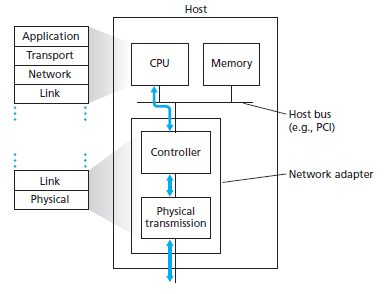
\includegraphics[width=0.85\linewidth]{cap18/nic_schema.png}
\end{minipage}\hfill
\begin{minipage}{0.45\linewidth}\centering
  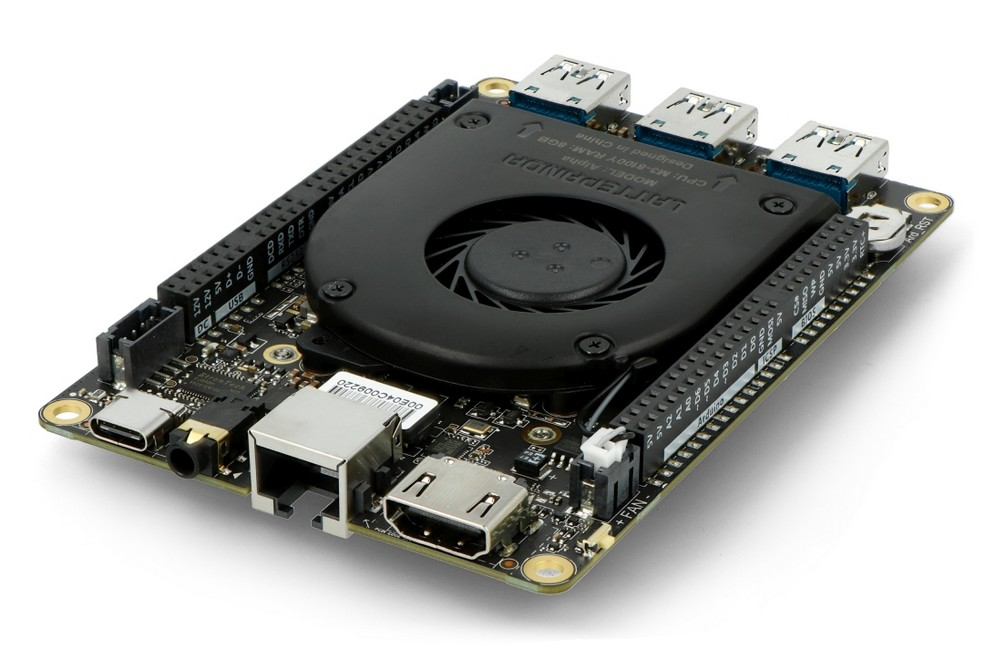
\includegraphics[width=0.85\linewidth]{cap18/nic.png}
\end{minipage}
\caption{A sinistra lo schema di un adattatore di rete collegato al bus dell'host; a destra un mini-PC (LattePanda) con la NIC integrata sulla scheda madre.}
\end{figure}

Nei computer ci sono adattatori di rete detti \textbf{NIC} (\emph{Network Interface Card}), con un chip specializzato
(\textbf{controller}) che realizza le funzioni di collegamento. Un tempo erano schede separate dalla scheda madre (inserite negli slot
PCI); oggi sono spesso integrate (\emph{LAN-on-motherboard}).

\subsection{Software e hardware}

\begin{itemize}
    \item \textbf{Software}: gira sulla CPU e offre funzioni di alto livello come l'indirizzamento, la gestione di interrupt e
          hardware, la gestione degli errori, l'incapsulamento e il decapsulamento dei datagrammi.
    \begin{itemize}
      \item A livello di collegamento c'è un indirizzo aggiuntivo, l'\textbf{indirizzo MAC}, che identifica la NIC.
      \item I datagrammi vanno letti dalla memoria in incapsulamento (lato mittente) e scritti in memoria in decapsulamento (lato
            ricevente), perché li usi il protocollo superiore.
    \end{itemize}
    \item \textbf{Hardware}: funziona come un tipico dispositivo di I/O, convertendo i dati nel segnale da trasmettere secondo il
          protocollo fisico (Ethernet, wireless, \dots).
\end{itemize}

\subsection{Le tecnologie fisiche}

Il protocollo di collegamento, e quindi la struttura del frame, dipende dalla tecnologia del collegamento fisico:

\begin{itemize}
    \item \textbf{Ethernet 802.3}: collegamento cablato basato su impulsi elettrici su cavi in rame con 4 doppini intrecciati (il più
          comune) o su fotoni in cavi di fibra ottica;
    \item \textbf{Wi-Fi 802.11}: collegamento senza fili a radiofrequenza (2,4 GHz, 5 GHz, 6 GHz);
    \item \textbf{Bluetooth}: collegamento senza fili a radiofrequenza (2,4 GHz).
\end{itemize}

\begin{table}[H]
\centering
\begin{tabular}{lllll}
\toprule
\textbf{Tipo} & \textbf{Segnale} & \textbf{Distanza} & \textbf{Banda} & \textbf{Punto debole} \\
\midrule
Senza fili & radio & 30--50 m & fino a 1,3 Gb/s & sicurezza, velocità \\
Doppino in rame & elettrico & 30--100 m & 1--25 Gb/s & interferenze \\
Fibra ottica & luce & 100--200 km & 1--400+ Gb/s & fragilità \\
\bottomrule
\end{tabular}
\caption{Pro e contro delle tecnologie fisiche (i limiti di distanza e banda cambiano continuamente).}
\end{table}

% ══════════════════════════════════════════════════════════════
\section{I metodi di framing}
% ══════════════════════════════════════════════════════════════

Potremmo trasmettere un flusso ininterrotto di bit? No: sarebbe impossibile \textbf{identificare gli errori} e
\textbf{ritrasmettere} solo le parti danneggiate. Inoltre bisogna distinguere i diversi pacchetti che arrivano come payload dal livello
di rete. Il ricevente deve quindi capire \textbf{dove inizia e dove finisce} ogni frame. I metodi principali sono quattro:

\begin{enumerate}
    \item conteggio dei byte (\emph{byte count});
    \item byte di flag con \emph{byte stuffing};
    \item bit di flag con \emph{bit stuffing};
    \item violazioni della codifica fisica.
\end{enumerate}

\subsection{Conteggio dei byte}

\dfn{Byte count}{
    Ogni frame inizia con un campo che indica il \textbf{numero di byte} del frame. È semplice, ma è difficilissimo
    risincronizzarsi dopo un errore, e in pratica non è mai usato da solo.
}

\begin{figure}[H]
\centering
\begin{tikzpicture}[every node/.style={font=\scriptsize\ttfamily}, b/.style={draw, minimum size=0.45cm, inner sep=0pt}]
  \node[font=\footnotesize\bfseries\sffamily, anchor=west] at (-0.5,0.7) {Senza errori};
  \foreach \v/\c [count=\i] in {5/netred!30,1/white,2/white,3/white,4/white, 5/netred!30,6/white,7/white,8/white,9/white, 8/netred!30,0/white,1/white,2/white,3/white,4/white,5/white,6/white, 8/netred!30,7/white,8/white,9/white,0/white,1/white,2/white,3/white}
     \node[b, fill=\c] at (\i*0.45,0) {\v};
  \draw[decorate, decoration={brace, amplitude=4pt, mirror}] (0.25,-0.35) -- (2.4,-0.35) node[midway, below=4pt, font=\scriptsize\sffamily] {frame 1: 5 byte};
  \draw[decorate, decoration={brace, amplitude=4pt, mirror}] (2.5,-0.35) -- (4.65,-0.35) node[midway, below=4pt, font=\scriptsize\sffamily] {frame 2: 5 byte};
  \draw[decorate, decoration={brace, amplitude=4pt, mirror}] (4.75,-0.35) -- (8.25,-0.35) node[midway, below=4pt, font=\scriptsize\sffamily] {frame 3: 8 byte};
  \draw[decorate, decoration={brace, amplitude=4pt, mirror}] (8.35,-0.35) -- (11.85,-0.35) node[midway, below=4pt, font=\scriptsize\sffamily] {frame 4: 8 byte};
  \begin{scope}[yshift=-2cm]
    \node[font=\footnotesize\bfseries\sffamily, anchor=west] at (-0.5,0.7) {Con un errore};
    \foreach \v/\c [count=\i] in {5/netred!30,1/white,2/white,3/white,4/white, 7/netorange!60,6/white,7/white,8/white,9/white, 8/white,0/white,1/white,2/white,3/white,4/white,5/white,6/white, 8/white,7/white,8/white,9/white,0/white,1/white,2/white,3/white}
       \node[b, fill=\c] at (\i*0.45,0) {\v};
    \draw[-{Stealth}, netorange, thick] (2.7,0.9) -- (2.7,0.3); \node[font=\scriptsize\sffamily, text=netorange] at (2.7,1.1) {errore: 5 diventa 7};
    \draw[decorate, decoration={brace, amplitude=4pt, mirror}] (2.5,-0.35) -- (5.55,-0.35) node[midway, below=4pt, font=\scriptsize\sffamily, text=netred] {frame 2 (sbagliato)};
    \draw[-{Stealth}, netred, thick] (5.85,-1.1) -- (5.85,-0.3); \node[font=\scriptsize\sffamily, text=netred, anchor=west] at (6,-1.0) {ora questo viene letto come un conteggio};
  \end{scope}
\end{tikzpicture}
\caption{Con il conteggio dei byte un solo errore sul contatore fa perdere la sincronizzazione su tutti i frame successivi.}
\end{figure}

\subsection{Byte di flag e byte stuffing}

\dfn{Byte stuffing}{
    Ogni frame è delimitato da uno speciale \textbf{byte di flag} (FLAG). Se il byte FLAG compare \textbf{nei dati}, va
    ``protetto'' inserendo prima di esso un byte di escape (ESC); lo stesso vale per un ESC che compare nei dati. Il ricevente
    rimuove ogni ESC e considera come dato il byte che lo segue.
}

\begin{figure}[H]
\centering
\begin{tikzpicture}[every node/.style={font=\scriptsize\sffamily}, b/.style={draw, minimum height=0.45cm, minimum width=0.75cm, inner sep=1pt}]
  \node[b, fill=netred!25] (f1) at (0,0) {FLAG}; \node[b, right=0pt of f1, minimum width=1.2cm] (hd) {header};
  \node[b, right=0pt of hd, minimum width=4cm] (pl) {payload}; \node[b, right=0pt of pl, minimum width=1.2cm] (tr) {trailer};
  \node[b, fill=netred!25, right=0pt of tr] {FLAG};
  \node[font=\footnotesize\sffamily\bfseries, anchor=east] at (-0.6,0) {formato del frame};
  \node[font=\footnotesize\bfseries\sffamily] at (2,-0.8) {dati originali}; \node[font=\footnotesize\bfseries\sffamily] at (7.2,-0.8) {dopo lo stuffing};
  \tikzset{bw/.style={b, fill=white}, by/.style={b, fill=llink!70}, bs/.style={b, fill=netred!20}}
  \foreach \row/\orig/\stuf in {
     0/{A/bw,FLAG/by,B/bw}/{A/bw,ESC/bs,FLAG/by,B/bw},
     1/{A/bw,ESC/by,B/bw}/{A/bw,ESC/bs,ESC/by,B/bw},
     2/{A/bw,ESC/by,FLAG/by,B/bw}/{A/bw,ESC/bs,ESC/by,ESC/bs,FLAG/by,B/bw},
     3/{A/bw,ESC/by,ESC/by,B/bw}/{A/bw,ESC/bs,ESC/by,ESC/bs,ESC/by,B/bw}} {
    \foreach \x/\st [count=\i] in \orig \node[\st] at (0.8+\i*0.75,-1.4-\row*0.65) {\x};
    \draw[-{Stealth}, thick] (4.2,-1.4-\row*0.65) -- (4.9,-1.4-\row*0.65);
    \foreach \x/\st [count=\i] in \stuf \node[\st] at (4.9+\i*0.75,-1.4-\row*0.65) {\x};
  }
\end{tikzpicture}
\caption{Byte stuffing: ogni FLAG o ESC nei dati viene preceduto da un ESC.}
\end{figure}

\begin{itemize}
    \item Il frame diventa \textbf{più lungo}, ma dopo un errore è \textbf{facile risincronizzarsi}: basta cercare il prossimo FLAG.
    \item Gli errori non si propagano come nel conteggio dei byte.
    \item In ricezione: ogni coppia ESC-FLAG diventa un FLAG di dati, ogni coppia ESC-ESC un ESC di dati.
\end{itemize}

\subsection{Bit di flag e bit stuffing}

\dfn{Bit stuffing}{
    Il flag che delimita i frame è la sequenza di bit \texttt{01111110} (sei 1 consecutivi). Per evitare che compaia nei dati:
    \begin{itemize}
      \item \textbf{in trasmissione}, dopo \textbf{cinque 1 consecutivi} nei dati si inserisce uno \textbf{0};
      \item \textbf{in ricezione}, ogni \textbf{0 che segue cinque 1} viene eliminato.
    \end{itemize}
}

\begin{figure}[H]
\centering
\begin{tikzpicture}[every node/.style={font=\small\ttfamily}]
  \node[anchor=east, font=\footnotesize\sffamily] at (-0.2,0) {dati};
  \node[anchor=west] at (0,0) {0110111111111111111110010};
  \node[anchor=east, font=\footnotesize\sffamily] at (-0.2,-0.8) {trasmessi};
  \node[anchor=west] at (0,-0.8) {011011111\textcolor{netred}{\textbf{0}}11111\textcolor{netred}{\textbf{0}}11111\textcolor{netred}{\textbf{0}}10010};
  \node[anchor=east, font=\footnotesize\sffamily] at (-0.2,-1.6) {ricevuti};
  \node[anchor=west] at (0,-1.6) {0110111111111111111110010};
  \node[font=\footnotesize\sffamily, text=netred, anchor=west] at (7.2,-0.8) {bit di stuffing inseriti};
\end{tikzpicture}
\caption{Bit stuffing: dopo cinque 1 si aggiunge uno 0, che il ricevente rimuove.}
\end{figure}

\subsection{Violazioni della codifica fisica}

Si sfrutta la codifica della trasmissione fisica: al livello fisico si usa un simbolo (o una parola) \textbf{che non rappresenta
dati}. Le violazioni della codifica delimitano i frame, e non serve alcuno stuffing, perché i simboli delimitatori \textbf{non possono
comparire} nei dati. È il caso, per esempio, della codifica 4B/5B, in cui alcune parole da 5 bit non sono mai usate per i dati.

% ══════════════════════════════════════════════════════════════
\section{La rilevazione degli errori}
% ══════════════════════════════════════════════════════════════

A livello di collegamento si possono rilevare e correggere gli errori a livello di singolo bit. In assenza di informazione
aggiuntiva non c'è nulla con cui confrontare il payload: bisogna aggiungerne.

\dfn{Il problema}{
    Siano $D$ i nostri dati, di $d$ bit. Per proteggerli dagli errori sui bit aggiungiamo al messaggio dei \textbf{bit di rilevazione
    e correzione degli errori}, \textbf{EDC} (\emph{Error Detection and Correction}). L'obiettivo è capire se i $D'$ ed $EDC'$
    ricevuti differiscono dagli originali $D$ ed $EDC$ e, se possibile, ricostruire gli originali.
}

\begin{figure}[H]
\centering
\begin{tikzpicture}[every node/.style={font=\scriptsize\sffamily}]
  \node[draw, fill=lnet!50, minimum width=1.4cm, minimum height=0.6cm] (dg) at (0,1) {datagramma};
  \node[draw, fill=llink!60, minimum width=1.2cm, minimum height=0.6cm, right=0pt of dg] {header link};
  \node[draw, fill=cloudbg, minimum width=2.6cm, minimum height=0.6cm] (d) at (0.6,0) {D};
  \node[draw, fill=netred!25, minimum width=0.8cm, minimum height=0.6cm, right=0pt of d] (e) {EDC};
  \node[draw, fill=cloudbg, minimum width=2.6cm, minimum height=0.6cm] (d2) at (9.2,0) {D'};
  \node[draw, fill=netred!25, minimum width=0.8cm, minimum height=0.6cm, right=0pt of d2] (e2) {EDC'};
  \draw[very thick, decorate, decoration={snake, amplitude=1.5pt, segment length=8pt}, -{Stealth}] (e.east) -- node[above=3pt] {collegamento soggetto a errori} (d2.west);
  \node[diamond, draw, aspect=2.5, fill=white, inner sep=1pt] (q) at (9.6,1.3) {D'+EDC' = D+EDC ?};
  \draw[-{Stealth}] (d2.north) -- (q);
\end{tikzpicture}
\caption{Il ricevente usa EDC' per verificare se D' è integro.}
\end{figure}

\warning{Nessuna garanzia assoluta}{
    Anche usando bit di rilevazione possono restare errori non rilevati, in casi ``patologici''. Le tecniche migliori riducono
    questa probabilità, ma al prezzo di più bit aggiuntivi e più calcoli.
}

% ══════════════════════════════════════════════════════════════
\section{Il controllo di parità}
% ══════════════════════════════════════════════════════════════

\dfn{Controllo di parità}{
    Il \textbf{controllo di parità} è la forma più semplice di rilevazione: si aggiunge al messaggio \textbf{un solo bit di parità},
    scelto in modo che il numero totale di 1 nei $d+1$ bit sia \textbf{pari} (schema a parità pari) o \textbf{dispari} (schema a parità
    dispari).
}

\begin{table}[H]
\centering
\begin{tabular}{lcc}
\toprule
\textbf{Messaggio} & \textbf{Bit di parità (pari)} & \textbf{Bit di parità (dispari)} \\
\midrule
\texttt{10101100} (quattro 1) & 0 & 1 \\
\texttt{11010000} (tre 1) & 1 & 0 \\
\bottomrule
\end{tabular}
\caption{Bit di parità pari e dispari.}
\end{table}

Il ricevente deve solo contare gli 1 nei $d+1$ bit ricevuti: se con uno schema pari trova un numero dispari di 1 (o viceversa), sa che
si è verificato \textbf{almeno un errore}.

\begin{esempio}{Un errore rilevato e uno no}
Si invia \texttt{10101100} con parità pari: \texttt{10101100 0}.
\begin{itemize}
    \item Si riceve \texttt{1010\textcolor{netred}{0}100 0}: tre 1, numero dispari $\Rightarrow$ \textbf{errore rilevato}.
    \item Si riceve \texttt{1010\textcolor{netred}{0}10\textcolor{netred}{1} 0}: quattro 1, numero pari $\Rightarrow$ due errori, \textbf{non rilevati}.
\end{itemize}
\end{esempio}

\warning{Gli errori arrivano a raffica}{
    La parità funziona solo se si verifica un numero \textbf{dispari} di errori. Quanto è probabile? Se gli errori sui bit fossero rari
    e indipendenti, la probabilità di errori multipli in un pacchetto sarebbe piccolissima. Ma nelle reti non è così: gli errori sono
    spesso \textbf{raggruppati a raffica} (\emph{burst}), cioè sequenze in cui il primo e l'ultimo bit sono sbagliati e quelli in mezzo sono
    un misto di bit sbagliati e corretti. In condizioni di burst la probabilità di errori non rilevati con la parità singola si avvicina al
    \textbf{50\%}: non è davvero utile.
}

\subsection{La parità bidimensionale}

\dfn{Parità bidimensionale}{
    Nella \textbf{parità bidimensionale} il messaggio viene diviso in $n$ righe e $m$ colonne, e a \textbf{ogni riga} e \textbf{ogni
    colonna} si associa un bit di parità.
}

\begin{figure}[H]
\centering
\begin{tikzpicture}[every node/.style={font=\small\ttfamily}, c/.style={draw, minimum size=0.5cm, inner sep=0pt}]
  \def\tabella#1#2#3{
    \begin{scope}[shift={#1}]
      \foreach \r [count=\i] in {#2} {
        \foreach \v [count=\j] in \r {
          \pgfmathsetmacro{\fillc}{(\i==5 || \j==6) ? "llink!60" : "white"}
          \node[c, fill=\fillc] (c\i\j) at (\j*0.5,-\i*0.5) {\v};
        }
      }
      #3
    \end{scope}
  }
  \node[font=\footnotesize\bfseries\sffamily] at (1.75,0.2) {senza errori};
  \tabella{(0,0)}{{1,0,1,0,1,1},{1,1,1,1,0,0},{0,1,1,1,0,1},{0,0,1,0,1,0},{0,0,0,0,0,0}}{}
  \node[font=\footnotesize\bfseries\sffamily] at (5.75,0.2) {un errore};
  \tabella{(4,0)}{{1,0,1,0,1,1},{1,0,1,1,0,0},{0,1,1,1,0,1},{0,0,1,0,1,0},{0,0,0,0,0,0}}{
     \draw[netred, very thick] (0.25,-1.25) rectangle (3.25,-0.75);
     \draw[netred, very thick] (0.75,-0.25) rectangle (1.25,-2.75);
     \node[circle, draw=netred, very thick, minimum size=0.55cm] at (1,-1) {};
  }
  \node[font=\footnotesize\bfseries\sffamily] at (9.75,0.2) {due errori};
  \tabella{(8,0)}{{1,0,1,0,1,1},{1,0,1,1,1,0},{0,1,1,1,0,1},{0,0,1,0,1,0},{0,0,0,0,0,0}}{
     \draw[netred, very thick] (0.75,-0.25) rectangle (1.25,-2.75);
     \draw[netred, very thick] (2.25,-0.25) rectangle (2.75,-2.75);
  }
  \node[font=\scriptsize\sffamily, text width=3cm, align=center] at (1.75,-3.2) {in giallo i bit di parità (pari)};
  \node[font=\scriptsize\sffamily, text width=3.4cm, align=center] at (5.75,-3.2) {riga 2 e colonna 2 sbagliate: il bit all'incrocio è quello errato e si può correggere};
  \node[font=\scriptsize\sffamily, text width=3.4cm, align=center] at (9.75,-3.2) {due colonne sbagliate, righe corrette: errore rilevato ma non correggibile};
\end{tikzpicture}
\caption{Parità bidimensionale: dati $4 \times 5$ bit, con parità di riga (ultima colonna) e di colonna (ultima riga).}
\end{figure}

\begin{itemize}
    \item Il ricevente può rilevare che si è verificato un errore e anche \textbf{quale bit} è sbagliato (all'incrocio tra la riga e la
          colonna con parità errata), e quindi tentare una \textbf{correzione}.
    \item La parità bidimensionale può anche \textbf{rilevare} (ma non correggere!) qualsiasi combinazione di \textbf{due errori} in un pacchetto.
\end{itemize}

% ══════════════════════════════════════════════════════════════
\section{Il CRC}
% ══════════════════════════════════════════════════════════════

\dfn{Cyclic Redundancy Check (CRC)}{
    Il \textbf{CRC} è una tecnica di rilevazione degli errori molto diffusa.
    \begin{itemize}
      \item Per inviare $d$ bit di dati $D$, mittente e ricevente concordano una sequenza di $r+1$ bit detta \textbf{generatore} $G$,
            con il bit più significativo (a sinistra) uguale a 1.
      \item Per ogni $D$ il mittente sceglie $r$ bit aggiuntivi, i \textbf{bit CRC} ($R$), da accodare al messaggio, in modo che il
            messaggio $M$ (cioè $D$ seguito da $R$) sia \textbf{divisibile modulo 2 per $G$} (resto = 0).
      \item Il ricevente divide il messaggio ricevuto per $G$: se il resto è zero il messaggio è corretto, altrimenti c'è un errore.
    \end{itemize}
    La divisione si esegue allineando $G$ sotto il primo bit a 1 del messaggio e facendo lo \textbf{XOR} bit a bit.
}

\subsection{L'aritmetica modulo 2}

Nel CRC le stringhe di bit sono interpretate come \textbf{polinomi a coefficienti binari}: \texttt{1011} è $x^3 + x + 1$. L'aritmetica
è modulo 2 senza riporti né prestiti: \textbf{somma e sottrazione coincidono con lo XOR}.

\begin{center}
\begin{tabular}{cc|c}
\toprule
$x$ & $y$ & $x \oplus y$ \\
\midrule
0 & 0 & 0 \\ 0 & 1 & 1 \\ 1 & 0 & 1 \\ 1 & 1 & 0 \\
\bottomrule
\end{tabular}
\end{center}

\info{Perché funziona (con i polinomi)}{
    Accodare $r$ zeri a $D$ equivale a moltiplicare $D(x)$ per $x^r$. Dividendo per il generatore si ottiene
    $$x^r D(x) = Q(x)\,G(x) + R(x)$$
    dove $Q$ è il quoziente e $R$ il resto (di grado minore di $r$). Allora il messaggio trasmesso
    $$M(x) = x^r D(x) - R(x) = x^r D(x) + R(x) = Q(x)\,G(x)$$
    è \textbf{divisibile per $G(x)$}. In binario, $M$ è semplicemente $D$ seguito dagli $r$ bit di $R$. Se durante la trasmissione si
    aggiunge un errore $E(x)$, il ricevente trova resto $\neq 0$ a meno che anche $E(x)$ sia divisibile per $G(x)$, cosa che un buon
    generatore rende molto improbabile.
}

\subsection{Un esempio completo}

Messaggio di 6 bit con CRC di 3 bit: $d = 6$, $D = \texttt{101110}$, $r = 3$, $G = \texttt{1001}$.

\begin{figure}[H]
\centering
\begin{minipage}{0.47\linewidth}
\centering\textbf{\small Mittente: calcolo del CRC}\\[4pt]
\begin{tabular}{r@{\,}l}
\multicolumn{2}{l}{\small $D$ con $r=3$ zeri: \texttt{101110\textcolor{netred}{000}}} \\[3pt]
& \texttt{\textbf{1}01110000} \\
XOR & \texttt{1001\phantom{00000}} \\ \cline{2-2}
& \texttt{00\textbf{1}01000\phantom{0}}\\[-2pt]
& \texttt{\phantom{00}101000\phantom{0}} \\
XOR & \texttt{\phantom{00}1001\phantom{000}} \\ \cline{2-2}
& \texttt{\phantom{00}00\textbf{1}100\phantom{0}} \\
XOR & \texttt{\phantom{0000}1001\phantom{0}} \\ \cline{2-2}
& \texttt{\phantom{0000}0\textbf{1}010} \\
XOR & \texttt{\phantom{00000}1001} \\ \cline{2-2}
& \texttt{\phantom{00000}0\textcolor{netred}{\textbf{011}}} \\
\end{tabular}\\[4pt]
{\small gli ultimi $r$ bit del resto sono il CRC: \textcolor{netred}{\texttt{011}}}
\end{minipage}\hfill
\begin{minipage}{0.47\linewidth}
\centering\textbf{\small Ricevente: verifica}\\[4pt]
\begin{tabular}{r@{\,}l}
\multicolumn{2}{l}{\small ricevuto $D$ + CRC: \texttt{101110\textcolor{netred}{011}}} \\[3pt]
& \texttt{\textbf{1}01110011} \\
XOR & \texttt{1001\phantom{00000}} \\ \cline{2-2}
& \texttt{00\textbf{1}01001\phantom{0}}\\[-2pt]
& \texttt{\phantom{00}101001\phantom{0}} \\
XOR & \texttt{\phantom{00}1001\phantom{000}} \\ \cline{2-2}
& \texttt{\phantom{00}00\textbf{1}101\phantom{0}} \\
XOR & \texttt{\phantom{0000}1001\phantom{0}} \\ \cline{2-2}
& \texttt{\phantom{0000}0\textbf{1}001} \\
XOR & \texttt{\phantom{00000}1001} \\ \cline{2-2}
& \texttt{\phantom{00000}0\textcolor{netgreen!60!black}{\textbf{000}}} \\
\end{tabular}\\[4pt]
{\small resto 0: il messaggio è integro}
\end{minipage}
\caption{Calcolo e verifica del CRC con $G = \texttt{1001}$: a ogni passo $G$ si allinea con il primo 1 rimasto.}
\end{figure}

\begin{enumerate}
    \item Il mittente accoda $r = 3$ zeri a $D$: \texttt{101110000}.
    \item Divide modulo 2 per $G$: allinea \texttt{1001} sotto il primo 1, fa lo XOR, poi si sposta sul primo 1 del risultato, e così via
          (spostamenti di 0, 2, 2 e 1 posizioni).
    \item Il resto, sugli ultimi $r$ bit, è \texttt{011}: è il CRC. Si trasmette \texttt{101110\,011}.
    \item Il ricevente divide per $G$ il messaggio ricevuto: il resto è \texttt{000}, quindi il messaggio è integro.
\end{enumerate}

\warning{Se c'è un errore}{
    Se durante la trasmissione un bit si inverte, per esempio si riceve \texttt{10\textcolor{netred}{0}110011}, la divisione dà un resto
    diverso da zero (qui \texttt{001}) e il ricevente scarta il frame. Provate a verificarlo!
}

\subsection{I CRC standard}

\begin{itemize}
    \item Sono stati definiti standard internazionali per generatori a 8, 12, 16 e 32 bit ($r = 8, 12, 16, 32$).
    \item Lo standard \textbf{CRC-32}, adottato in diversi protocolli di collegamento IEEE (tra cui Ethernet), usa il generatore a 33 bit:
          $$G_{\text{CRC-32}} = \texttt{100000100110000010001110110110111}$$
    \item Ogni standard CRC rileva \textbf{sicuramente} tutti gli errori a raffica di lunghezza inferiore a $r+1$ bit; per raffiche più
          lunghe la probabilità di rilevare l'errore è
          $$P = 1 - 0{,}5^{\,r}$$
    \item La probabilità di rilevare l'errore quindi \textbf{cresce con $r$}: con CRC-32 si perde un errore su circa quattro miliardi.
\end{itemize}

% ══════════════════════════════════════════════════════════════
\section{La distanza di Hamming}
% ══════════════════════════════════════════════════════════════

Oltre a rilevare gli errori, alcuni codici permettono di \textbf{correggerli}.

\dfn{Codice e distanza di Hamming}{
    Un codice trasforma dati di $n$ bit in \textbf{parole di codice} (\emph{codeword}) di $n + k$ bit. La \textbf{distanza di Hamming}
    tra due parole è il numero di bit che è necessario invertire per trasformare una nell'altra, cioè il numero di bit in cui
    differiscono. La distanza di Hamming \textbf{di un codice} è la \textbf{minima} distanza tra due parole valide qualsiasi del codice.
}

\begin{esempio}{Distanza tra due parole}
$w_1 = \texttt{00110110}$, $w_2 = \texttt{00011010}$. Facendo lo XOR,
$w_1 \oplus w_2 = \texttt{00101100}$: i bit diversi sono 3, quindi $d(w_1, w_2) = 3$.
\end{esempio}

I protocolli di collegamento usano per comunicare parole di lunghezza fissa che \textbf{non sono tutte quelle possibili}. Per esempio,
delle $2^5$ parole possibili di 5 bit se ne usano $2^4$ (la metà), come nella codifica \textbf{4B/5B}. Ciò consente di rilevare gli
errori, e anche di evitare lunghe sequenze di 1 o di 0 (utili per la sincronizzazione).

\begin{esempio}{Un codice con distanza 5}
Usiamo parole di 10 bit, ma ne usiamo solo 4 (per codificare 2 bit di dati, $n=2$, $k=8$):
\begin{center}
\begin{tabular}{cc}
\toprule
\textbf{Dati} & \textbf{Parola di codice} \\
\midrule
00 & \texttt{0000000000} \\
01 & \texttt{0000011111} \\
10 & \texttt{1111100000} \\
11 & \texttt{1111111111} \\
\bottomrule
\end{tabular}
\end{center}
La distanza minima tra due parole è \textbf{5}. Se si riceve \texttt{0000011111}, è una parola valida. Se si riceve
\texttt{0\textcolor{netred}{1}000111\textcolor{netred}{0}1}, non è valida: è a distanza 2 da \texttt{0000011111} e a distanza maggiore da tutte
le altre, quindi si \textbf{corregge} in \texttt{0000011111} (dato 01). Si è trattato di uno schema didattico (v. Tanenbaum per i veri
codici di Hamming, basati su questo principio ma più complicati).
\end{esempio}

\dfn{Capacità di rilevazione e correzione}{
    Con un codice di distanza di Hamming $L$:
    \begin{itemize}
      \item si possono \textbf{rilevare} fino a $d$ errori se $L \geq d + 1$ (cioè $d \leq L - 1$): $d$ errori non bastano a trasformare
            una parola valida in un'altra;
      \item si possono \textbf{correggere} fino a $d$ errori se $L \geq 2d + 1$: la parola ricevuta resta più vicina a quella originale che
            a qualsiasi altra.
    \end{itemize}
    Nell'esempio ($L = 5$): si rilevano fino a 4 errori e se ne correggono fino a 2.
}

\begin{figure}[H]
\centering
\begin{tikzpicture}[every node/.style={font=\scriptsize\sffamily}]
  \draw[thick] (0,0) -- (10,0);
  \fill[netblue] (0,0) circle (4pt) node[below=5pt] {$w$ (valida)};
  \fill[netblue] (10,0) circle (4pt) node[below=5pt] {$w'$ (valida)};
  \foreach \x in {2,4,6,8} \fill[black!40] (\x,0) circle (2.5pt);
  \draw[decorate, decoration={brace, amplitude=6pt, mirror}] (0,-0.7) -- (10,-0.7) node[midway, below=7pt] {distanza $L = 5$};
  \fill[netred!20] (0,0.25) rectangle (4.9,0.55); \node[text=netred] at (2.45,0.85) {parole ricevute che si correggono in $w$};
  \fill[netgreen!20] (5.1,0.25) rectangle (10,0.55); \node[text=netgreen!50!black] at (7.55,0.85) {parole ricevute che si correggono in $w'$};
  \draw[-{Stealth}, netred, thick] (4,-0.15) to[bend right=30] node[below] {2 errori} (0,-0.15);
\end{tikzpicture}
\caption{Con distanza 5, una parola con al massimo 2 errori è ancora più vicina all'originale: si può correggere.}
\end{figure}

% ══════════════════════════════════════════════════════════════
\section{Riepilogo}
% ══════════════════════════════════════════════════════════════

\riepilogo{
\begin{itemize}
    \item Collegamento e fisico trasportano frame \textbf{da un nodo al successivo}; il frame è l'ultimo incapsulamento e diventa segnale.
    \item Servizi: \textbf{framing}, \textbf{accesso al collegamento} (MAC), \textbf{consegna affidabile}, \textbf{rilevazione e correzione}
          degli errori. Realizzati soprattutto nella \textbf{NIC}.
    \item Framing: conteggio dei byte (fragile), FLAG con \textbf{byte stuffing}, flag \texttt{01111110} con \textbf{bit stuffing}, violazioni della codifica.
    \item \textbf{Parità} singola (rileva un numero dispari di errori), \textbf{bidimensionale} (corregge 1 errore, rileva 2).
    \item \textbf{CRC}: si accodano $r$ bit perché $D\cdot 2^r + R$ sia divisibile modulo 2 per $G$; rileva le raffiche $< r+1$.
    \item Distanza di Hamming $L$: rileva $L-1$ errori, ne corregge $\lfloor (L-1)/2 \rfloor$.
\end{itemize}
}
  % Framing ed errori
  \chapter{Il sottolivello MAC e l'accesso multiplo}

% ══════════════════════════════════════════════════════════════
\section{I due tipi di collegamento}
% ══════════════════════════════════════════════════════════════

Ricordiamo i quattro servizi del livello di collegamento: \textbf{framing} (incapsulare e decapsulare i datagrammi), \textbf{accesso al
collegamento} (regolare l'accesso ai collegamenti condivisi, compito del protocollo MAC), \textbf{consegna affidabile} (per lo più
facoltativa) e \textbf{rilevazione e correzione degli errori} (parità, checksum, CRC). In questo capitolo ci occupiamo del secondo.

I collegamenti da gestire sono essenzialmente di due tipi.

\dfn{Collegamento punto-punto e broadcast}{
    \begin{itemize}
      \item Un collegamento \textbf{punto-punto} ha un solo mittente a un'estremità e un solo ricevente all'altra. Un protocollo che
            gestisce collegamenti di questo tipo è il \textbf{PPP} (\emph{Point-to-Point Protocol}). Esempio: un cavo Ethernet diretto
            tra due computer.
      \item Un collegamento \textbf{broadcast} ha più nodi mittenti e riceventi collegati allo \textbf{stesso canale condiviso}. Si
            chiama broadcast perché quando un nodo trasmette un frame, questo viene \textbf{ricevuto da tutti} i nodi sul canale.
            Esempi: il bus Ethernet, Ethernet half-duplex (raro, oggi i cavi sono quasi tutti full-duplex), le LAN wireless.
    \end{itemize}
}

\begin{figure}[H]
\centering
\begin{tikzpicture}[every node/.style={font=\footnotesize\sffamily}]
  \begin{scope}
    \node[font=\small\bfseries\sffamily] at (2,1.6) {Punto-punto};
    \node (a) at (0,0) {\icon[1cm]{pc}}; \node[below=-2pt of a] {invia A};
    \node (b) at (4,0) {\icon[1cm]{laptop}}; \node[below=-2pt of b, text=netgreen!60!black] {accetta A};
    \draw[wired, line width=1.6pt] (a) -- node[above] {PPP} (b);
  \end{scope}
  \begin{scope}[xshift=7.5cm]
    \node[font=\small\bfseries\sffamily] at (2.5,1.6) {Broadcast};
    \draw[backbone] (-0.2,0) -- (5.2,0);
    \foreach \x/\ic/\t/\c in {0/pc/{invia A}/black, 1.7/laptop/{scarta A}/netred, 3.4/pc/{accetta A}/netgreen!60!black, 5/laptop/{scarta A}/netred} {
      \node (n) at (\x,0.8) {\icon[0.7cm]{\ic}}; \draw[wired] (\x,0) -- (n);
      \node[text=\c] at (\x,-0.4) {\t};
    }
  \end{scope}
\end{tikzpicture}
\caption{Nel broadcast tutti ricevono il frame, e solo il destinatario lo accetta.}
\end{figure}

L'accesso ai collegamenti broadcast va \textbf{coordinato} (\emph{problema dell'accesso multiplo}), perché più comunicazioni sullo
stesso collegamento possono interferire tra loro.

% ══════════════════════════════════════════════════════════════
\section{Le collisioni}
% ══════════════════════════════════════════════════════════════

\dfn{Collisione}{
    Il problema principale dei collegamenti broadcast è la \textbf{collisione}: se più nodi trasmettono frame \textbf{contemporaneamente}
    sullo stesso canale, i frame si sovrappongono e diventano \textbf{incomprensibili}.
}

I frame in collisione vengono ricevuti da tutti i nodi e scartati come errati (non si fa danno), ma:

\begin{itemize}
    \item \textbf{tutti} i frame trasmessi vanno \textbf{persi};
    \item l'intervallo di tempo è \textbf{sprecato}, perché il canale è stato usato per trasmettere dati inutili.
\end{itemize}

\begin{figure}[H]
\centering
\begin{tikzpicture}[every node/.style={font=\footnotesize\sffamily}]
  \draw[backbone] (-0.2,0) -- (8.2,0);
  \node (a) at (0,0.8) {\icon[0.7cm]{pc}}; \draw[wired] (0,0) -- (a); \node[above=-1pt of a] {invia A};
  \node (b) at (8,0.8) {\icon[0.7cm]{pc}}; \draw[wired] (8,0) -- (b); \node[above=-1pt of b] {invia B};
  \node (c) at (2.7,0.8) {\icon[0.8cm]{laptop}}; \draw[wired] (2.7,0) -- (c); \node[above=-1pt of c, text=netred] {scarta \$@!};
  \node (d) at (5.3,0.8) {\icon[0.8cm]{laptop}}; \draw[wired] (5.3,0) -- (d); \node[above=-1pt of d, text=netred] {scarta \$@!};
  \draw[-{Stealth}, very thick, netblue] (0.3,-0.3) -- (4.8,-0.3);
  \draw[-{Stealth}, very thick, netorange] (7.7,-0.45) -- (3.2,-0.45);
  \node[starburst, draw=netred, fill=netred!20, minimum size=0.9cm, inner sep=0pt, font=\scriptsize\bfseries\sffamily] at (4,-0.9) {collisione!};
\end{tikzpicture}
\caption{Due trasmissioni contemporanee sullo stesso canale collidono: tutti i nodi ricevono dati illeggibili.}
\end{figure}

L'accesso al mezzo fisico (come il framing) è regolato dal protocollo \textbf{MAC} (\emph{Medium Access Control}), un
\textbf{sottolivello} del livello di collegamento.

% ══════════════════════════════════════════════════════════════
\section{I protocolli ad accesso multiplo}
% ══════════════════════════════════════════════════════════════

Nelle reti i \textbf{protocolli ad accesso multiplo} regolano le trasmissioni sui canali broadcast in modo che:

\begin{itemize}
    \item le collisioni siano \textbf{gestite};
    \item ogni nodo abbia la possibilità di trasmettere, e nessuno \textbf{monopolizzi} il collegamento;
    \item le connessioni già stabilite non vengano interrotte (per esempio controllando se il collegamento è occupato).
\end{itemize}

Servono in molti contesti, cablati, senza fili e satellitari, dove centinaia o migliaia di nodi possono comunicare direttamente su un
canale broadcast. Ne esistono decine, su tecnologie di collegamento diverse; gli approcci principali sono tre:

\begin{itemize}
    \item \textbf{partizionamento del canale}: la banda viene divisa tra i nodi;
    \item \textbf{accesso casuale}: i nodi ``tentano la sorte'' per accedere;
    \item \textbf{a turni} (\emph{taking-turns}): i nodi aspettano il proprio turno.
\end{itemize}

\dfn{Le proprietà desiderate}{
    Un protocollo ad accesso multiplo per un canale broadcast a $R$ bit/s dovrebbe essere:
    \begin{itemize}
      \item \textbf{efficiente}: se un solo nodo deve trasmettere, dovrebbe avere throughput $R$; se $M$ nodi devono trasmettere, ciascuno
            dovrebbe avere in media $R/M$ bit/s;
      \item \textbf{decentralizzato}: un nodo ``master'' sarebbe un single point of failure;
      \item \textbf{semplice e leggero}: si inviano tantissimi frame, non ci può essere overhead.
    \end{itemize}
}

% ══════════════════════════════════════════════════════════════
\section{Protocolli a partizionamento del canale}
% ══════════════════════════════════════════════════════════════

\subsection{TDMA}

\dfn{TDMA (Time Division Multiple Access)}{
    Dato un canale con $N$ nodi e velocità $R$ bit/s, il \textbf{TDMA} divide il tempo in \textbf{trame} (\emph{frame} temporali) e ogni
    trama in $N$ \textbf{slot}. Ogni slot è assegnato a uno degli $N$ nodi: quando un nodo ha un pacchetto da inviare, aspetta il proprio
    slot. Di solito la dimensione degli slot è scelta in modo che un pacchetto intero possa essere trasmesso in uno slot.
}

\subsection{FDMA}

\dfn{FDMA (Frequency Division Multiple Access)}{
    Il \textbf{FDMA} divide il canale da $R$ bit/s in \textbf{frequenze diverse}, ciascuna con banda $R/N$, e assegna ogni frequenza a uno
    degli $N$ nodi.
}

\begin{figure}[H]
\centering
\begin{tikzpicture}[every node/.style={font=\scriptsize\sffamily}]
  \begin{scope}
    \node[font=\footnotesize\bfseries\sffamily] at (2.8,2.6) {TDMA};
    \draw[-{Stealth}] (0,0) -- (6,0) node[right] {tempo}; \draw[-{Stealth}] (0,0) -- (0,2.3) node[above] {frequenza};
    \foreach \k in {0,1} \foreach \i/\c in {1/lapp,2/ltra,3/lnet,4/llink} { \fill[\c] (0.1+\k*2.8+\i*0.65-0.65,0.1) rectangle ++(0.6,1.9); \node at (0.4+\k*2.8+\i*0.65-0.65,1.05) {N\i}; }
    \draw[decorate, decoration={brace, amplitude=4pt, mirror}] (0.1,-0.15) -- (2.7,-0.15) node[midway, below=4pt] {trama};
    \draw[decorate, decoration={brace, amplitude=3pt}] (0.1,2.05) -- (0.7,2.05) node[midway, above=3pt] {slot};
  \end{scope}
  \begin{scope}[xshift=7.8cm]
    \node[font=\footnotesize\bfseries\sffamily] at (2.8,2.6) {FDMA};
    \draw[-{Stealth}] (0,0) -- (6,0) node[right] {tempo}; \draw[-{Stealth}] (0,0) -- (0,2.3) node[above] {frequenza};
    \foreach \i/\c in {1/lapp,2/ltra,3/lnet,4/llink} { \fill[\c] (0.1,0.1+\i*0.48-0.48) rectangle ++(5.6,0.44); \node at (2.9,0.32+\i*0.48-0.48) {N\i}; }
  \end{scope}
\end{tikzpicture}
\caption{TDMA: a turno, ciascuno con tutta la banda. FDMA: sempre, ciascuno con una fetta della banda.}
\end{figure}

FDMA e TDMA condividono pro e contro:

\begin{itemize}
    \item[\itick] \textbf{evitano le collisioni} e dividono la banda \textbf{equamente} tra gli $N$ nodi;
    \item[\icross] un nodo è limitato a una banda di $R/N$ \textbf{anche quando è l'unico} ad avere pacchetti da inviare: capacità sprecata.
\end{itemize}

\subsection{CDMA}

\dfn{CDMA (Code Division Multiple Access)}{
    Il \textbf{CDMA} assegna a ogni nodo un \textbf{codice} diverso, con cui codifica e decodifica i bit che invia. Se i codici sono scelti con
    cura, nelle reti CDMA più nodi possono trasmettere \textbf{contemporaneamente, sulle stesse frequenze}, senza interferire.
}

\begin{esempio}{L'idea del CDMA}
Siano $c_A = (+1, -1)$ e $c_B = (+1, +1)$ i codici di due stazioni: sono \textbf{ortogonali}, cioè il loro prodotto scalare è
$c_A \cdot c_B = 1 - 1 = 0$, mentre $c_B \cdot c_B = 2$. Per trasmettere un bit, ogni stazione invia il proprio codice moltiplicato per
$+1$ (bit 1) o $-1$ (bit 0). Sul canale i segnali si \textbf{sommano}.
\begin{itemize}
    \item A invia 1, B invia 1: sul canale arriva $c_A + c_B = (2, 0)$.
    \item Il ricevente di B calcola $(c_A + c_B)\cdot c_B = c_A\cdot c_B + c_B \cdot c_B = 0 + 2 > 0$: B ha inviato \textbf{1}.
    \item Il ricevente di A calcola $(c_A + c_B)\cdot c_A = 2 + 0 > 0$: anche A ha inviato \textbf{1}.
\end{itemize}
Il contributo dell'altra stazione si annulla grazie all'ortogonalità dei codici (v. Tanenbaum per i dettagli).
\end{esempio}

\begin{itemize}
    \item Funziona soprattutto sui canali \textbf{senza fili}; è usato da tempo in ambito militare (per le sue proprietà anti-disturbo) e
          nella telefonia cellulare (per esempio il 3G).
    \item[\icross] È complesso da realizzare.
    \item[\icross] Non scala bene con il numero di nodi.
\end{itemize}

\info{Il segnale modulato}{
    Sui canali radio i dati non viaggiano ``così come sono'': si trasmette un segnale in \textbf{banda base} (a bassa frequenza) modulando una
    \textbf{frequenza portante} più alta. Il telefono analogico, per esempio, usa la banda 300--3400 Hz. FDMA e CDMA lavorano proprio sulle
    frequenze portanti e sulla loro condivisione.
}

% ══════════════════════════════════════════════════════════════
\section{Protocolli ad accesso casuale}
% ══════════════════════════════════════════════════════════════

\dfn{Accesso casuale}{
    Nei protocolli ad \textbf{accesso casuale} un nodo che trasmette usa sempre \textbf{tutta la velocità} del canale ($R$ bit/s). Se avviene
    una collisione (almeno due nodi trasmettono insieme), ogni nodo coinvolto \textbf{aspetta un ritardo casuale} prima di ritrasmettere.
}

Poiché la scelta del ritardo è fatta indipendentemente, è possibile che i due nodi scelgano ritardi abbastanza diversi da permettere a uno
dei due di ``infilare'' il proprio messaggio. Se invece scelgono ritardi simili, avviene una nuova collisione e il processo si ripete.

\subsection{ALOHA puro}

Il primo protocollo ad accesso casuale nacque alle Hawaii (ALOHAnet, anni '70), per collegare le isole via radio:

\begin{itemize}
    \item ogni stazione trasmette \textbf{appena ha un frame} da inviare;
    \item una stazione centrale ripete ogni frame ricevuto: se non ci sono collisioni, ogni stazione riceve indietro il frame che ha appena
          trasmesso, e capisce così se è arrivato;
    \item in caso di collisione si attende un tempo di lunghezza casuale e si ritrasmette.
\end{itemize}

\begin{figure}[H]
\centering
\begin{tikzpicture}[every node/.style={font=\scriptsize\sffamily}]
  \foreach \y/\n in {0/A, -0.7/B, -1.4/C} { \node[anchor=east] at (-0.2,\y) {\n}; \draw[black!30] (0,\y) -- (11,\y); }
  \draw[-{Stealth}] (0,-1.9) -- (11,-1.9) node[right] {tempo};
  \fill[netblue!40] (0.5,-0.2) rectangle (2.5,0.2);
  \fill[netred!40] (2.0,-0.9) rectangle (4.0,-0.5); \fill[netred!40] (3.4,-1.6) rectangle (5.4,-1.2);
  \fill[netblue!40] (5.8,-0.2) rectangle (7.8,0.2); \fill[netblue!40] (8.4,-0.9) rectangle (10.4,-0.5);
  \draw[netred, very thick] (2.0,-1.05) -- (5.4,-1.05);
  \node[text=netred] at (3.7,-2.25) {B e C si sovrappongono (e B anche con A): collisioni};
  \draw[dashed] (2,0.4) -- (2,-1.9); \draw[dashed] (2.5,0.4) -- (2.5,-1.9);
\end{tikzpicture}
\caption{ALOHA puro: basta che due frame si sovrappongano anche in parte perché entrambi vadano persi.}
\end{figure}

\subsection{Slotted ALOHA}

\dfn{Slotted ALOHA}{
    \begin{itemize}
      \item Il tempo è diviso in \textbf{slot} (come in TDMA), ciascuno grande abbastanza da contenere un frame.
      \item I nodi sono \textbf{sincronizzati}: ogni nodo trasmette frame solo \textbf{all'inizio} di uno slot.
      \item Se nello slot non c'è collisione, la comunicazione prosegue.
      \item Se c'è una collisione, ogni nodo coinvolto ritrasmette il frame in ciascuno degli slot successivi \textbf{con probabilità
            $p \in [0,1]$} (``lancia una moneta''), finché il frame non viene inviato con successo.
    \end{itemize}
}

\begin{figure}[H]
\centering
\begin{tikzpicture}[every node/.style={font=\scriptsize\sffamily}]
  \foreach \x in {0,1.5,...,9} \draw[dashed, black!30] (\x,0.6) -- (\x,-1.6);
  \node[anchor=east] at (-0.2,0) {nodo 1}; \node[anchor=east] at (-0.2,-1) {nodo 2};
  \draw[-{Stealth}] (0,-1.6) -- (9.3,-1.6) node[right] {tempo};
  \fill[netred!40] (0,-0.2) rectangle (1.5,0.2); \fill[netred!40] (0,-1.2) rectangle (1.5,-0.8);
  \node[text=netred] at (0.75,-0.5) {collisione};
  \node at (2.25,0) {non invia}; \node at (2.25,-1) {non invia};
  \fill[netred!40] (3,-0.2) rectangle (4.5,0.2); \fill[netred!40] (3,-1.2) rectangle (4.5,-0.8);
  \node[text=netred] at (3.75,-0.5) {collisione};
  \fill[netgreen!40] (4.5,-0.2) rectangle (6,0.2); \node at (5.25,0) {invia};
  \node at (5.25,-1) {non invia};
  \fill[netgreen!40] (7.5,-1.2) rectangle (9,-0.8); \node at (8.25,-1) {invia};
  \node[text=netgreen!50!black] at (5.25,0.45) {successo}; \node[text=netgreen!50!black] at (8.25,-0.55) {successo};
\end{tikzpicture}
\caption{Slotted ALOHA: dopo una collisione, in ogni slot ciascun nodo ritrasmette con probabilità $p$.}
\end{figure}

\begin{itemize}
    \item[\itick] Se c'è un solo nodo, usa tutta la velocità $R$ del canale (niente collisioni).
    \item[\itick] È \textbf{decentralizzato}: i nodi sono del tutto indipendenti tra loro, a parte la sincronizzazione.
    \item[\itick] È \textbf{semplice} da realizzare ed eseguire (la scelta casuale è velocissima).
    \item[\itick] Più collisioni consecutive sono improbabili.
\end{itemize}

\begin{figure}[H]
\centering
\begin{tikzpicture}
  \begin{axis}[width=10cm, height=5cm, xlabel={$G$ (tentativi per slot, cioè per tempo di frame)}, ylabel={$S$ (throughput per frame)},
      xmin=0, xmax=3, ymin=0, ymax=0.42, grid=major, grid style={gray!20}, legend pos=north east,
      legend style={font=\scriptsize\sffamily}, tick label style={font=\scriptsize}, label style={font=\footnotesize\sffamily}]
    \addplot[very thick, netblue, domain=0:3, samples=80] {x*exp(-x)}; \addlegendentry{slotted ALOHA: $S = Ge^{-G}$}
    \addplot[very thick, netred, domain=0:3, samples=80] {x*exp(-2*x)}; \addlegendentry{ALOHA puro: $S = Ge^{-2G}$}
    \addplot[only marks, mark=*, netblue] coordinates {(1,0.368)}; \addplot[only marks, mark=*, netred] coordinates {(0.5,0.184)};
  \end{axis}
\end{tikzpicture}
\caption{Throughput di ALOHA: al meglio lo slotted ALOHA usa il canale per il 37\% del tempo ($1/e$), l'ALOHA puro solo il 18\% ($1/2e$).}
\end{figure}

\subsection{CSMA e CSMA/CD}

Un punto debole di ALOHA è che si può cominciare a trasmettere (producendo una collisione) anche se il canale \textbf{è già occupato}: ce
ne accorgiamo solo dall'effetto delle collisioni. La soluzione è \textbf{ascoltare} il canale e tentare di trasmettere solo se è libero.

\dfn{CSMA e CSMA/CD}{
    I protocolli \textbf{CSMA} (\emph{Carrier Sense Multiple Access}) e \textbf{CSMA/CD} (CSMA con \emph{Collision Detection}) si basano su
    due principi:
    \begin{itemize}
      \item \textbf{carrier sensing}: i nodi ascoltano il canale \textbf{prima} di trasmettere. Se un altro nodo sta trasmettendo un frame,
            aspettano che la trasmissione finisca;
      \item \textbf{collision detection}: i nodi ascoltano il canale \textbf{mentre} trasmettono. Se rilevano una collisione, smettono di
            trasmettere e aspettano un tempo casuale prima di riprovare.
    \end{itemize}
}

Ma se tutti i nodi ascoltano prima di trasmettere, perché avvengono comunque collisioni? Per il \textbf{ritardo di propagazione} del
segnale.

\begin{figure}[H]
\centering
\begin{minipage}{0.34\linewidth}\centering
  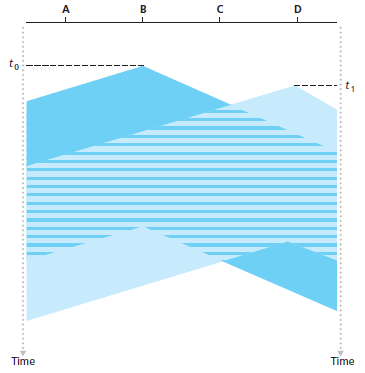
\includegraphics[width=0.9\linewidth]{cap19/csma_ritardo.png}
\end{minipage}\hfill
\begin{minipage}{0.62\linewidth}
\begin{itemize}
  \item Anche se la propagazione è vicina alla velocità della luce, il segnale impiega del \textbf{tempo} per raggiungere gli altri nodi.
  \item Nella figura (spazio in orizzontale, tempo verso il basso) B comincia a trasmettere al tempo $t_0$ e il segnale si propaga in entrambe
        le direzioni. Al tempo $t_1$ D non ha ancora ricevuto il segnale di B, ascolta, trova il canale libero e \textbf{inizia a trasmettere}.
  \item Poco dopo i due segnali si incontrano: collisione. D se ne accorge solo quando riceve il segnale di B.
\end{itemize}
Per questo ritardo tra inizio della trasmissione e rilevazione, un nodo può considerare libero un canale che in realtà è già in uso.
\end{minipage}
\caption{Collisione in CSMA dovuta al ritardo di propagazione (da Kurose).}
\end{figure}

\subsubsection*{CSMA puro}

\begin{enumerate}
    \item Controlla se il canale è occupato.
    \item Se il canale è libero, invia un frame.
\end{enumerate}

In CSMA puro le collisioni \textbf{non vengono rilevate}, anche se sono possibili: si capisce che un frame è andato perso solo perché
\textbf{non arriva l'ACK}.

\info{Varianti di CSMA}{
    Cosa fare se il canale è occupato? Nel \textbf{CSMA 1-persistente} si aspetta che si liberi e si trasmette subito (con probabilità 1);
    nel \textbf{non persistente} si attende un tempo casuale e si riascolta; nel \textbf{$p$-persistente} (su canali a slot), quando il canale è
    libero si trasmette con probabilità $p$ e si rimanda allo slot successivo con probabilità $1-p$.
}

\subsubsection*{CSMA/CD}

Il \textbf{CSMA/CD}, più sofisticato, è quello implementato in \textbf{Ethernet}:

\begin{enumerate}
    \item controlla se il canale è occupato;
    \item se il canale è libero, invia un frame;
    \item \textbf{durante la trasmissione} controlla eventuali collisioni;
    \item se rileva una collisione, \textbf{smette subito} di trasmettere e attende un periodo casuale $K \cdot$ (tempo di slot), con
          $K \in \{0, 1, \dots, 2^n - 1\}$, dove $n$ è il numero di collisioni già rilevate per quel frame (\textbf{binary exponential backoff}).
\end{enumerate}

\begin{figure}[H]
\centering
\begin{tikzpicture}[every node/.style={font=\scriptsize\sffamily}]
  \draw[-{Stealth}] (0,0) -- (13,0) node[right] {tempo};
  \fill[netblue!40] (0.2,0.1) rectangle (3,0.7); \node at (1.6,0.4) {frame};
  \fill[netred!30] (3.3,0.1) rectangle (3.8,0.7); \fill[netred!30] (4.0,0.1) rectangle (4.5,0.7); \fill[netred!30] (4.7,0.1) rectangle (5.2,0.7);
  \draw[decorate, decoration={brace, amplitude=4pt}] (3.3,0.8) -- (5.2,0.8) node[midway, above=4pt, align=center] {periodo di contesa:\\collisioni brevi, interrotte};
  \fill[netblue!40] (5.5,0.1) rectangle (8.3,0.7); \node at (6.9,0.4) {frame};
  \fill[black!10] (8.5,0.1) rectangle (10,0.7); \node at (9.25,0.4) {inattivo};
  \fill[netblue!40] (10.2,0.1) rectangle (12.8,0.7); \node at (11.5,0.4) {frame};
\end{tikzpicture}
\caption{Con la collision detection le collisioni durano pochissimo: le stazioni smettono appena se ne accorgono, e il canale torna disponibile.}
\end{figure}

\begin{esempio}{Il binary exponential backoff}
\begin{itemize}
    \item Dopo la \textbf{1\textsuperscript{a}} collisione: $K \in \{0, 1\}$.
    \item Dopo la \textbf{2\textsuperscript{a}}: $K \in \{0, 1, 2, 3\}$.
    \item Dopo la \textbf{3\textsuperscript{a}}: $K \in \{0, \dots, 7\}$; dopo la $n$-esima: $K \in \{0, \dots, 2^n - 1\}$ (in Ethernet $n$ si ferma a 10).
\end{itemize}
Se due stazioni collidono una prima volta, con probabilità 1/2 scelgono lo stesso $K$ e collidono di nuovo; alla seconda la probabilità scende
a 1/4, poi a 1/8. La probabilità di riuscire a inviare il frame \textbf{cresce con il numero di collisioni}, adattando l'attesa al carico: con
poche stazioni le attese sono brevi, con molte si allungano.
\end{esempio}

\warning{La lunghezza minima dei frame in Ethernet}{
    Perché la collision detection funzioni, una stazione deve essere \textbf{ancora in trasmissione} quando le arriva il segnale della collisione.
    Sia $\tau$ il tempo di propagazione tra le due stazioni più lontane. Nel caso peggiore A inizia al tempo 0, e il suo segnale arriva a B al tempo
    $\tau - \varepsilon$, un attimo dopo che B ha iniziato a trasmettere; B rileva subito la collisione, ma il ``rumore'' della collisione torna ad
    A solo al tempo $2\tau - \varepsilon$. Quindi il tempo di trasmissione di un frame deve essere di almeno $2\tau$: per questo Ethernet ha un
    campo \textbf{pad} che allunga artificialmente i frame troppo corti (dati da almeno 46 byte).
    \begin{center}
    \begin{tikzpicture}[every node/.style={font=\scriptsize\sffamily}]
      \node[draw, minimum size=0.5cm] (A) at (0,0) {A}; \node[draw, minimum size=0.5cm] (B) at (6,0) {B};
      \draw[thick] (A) -- (B);
      \draw[-{Stealth}, netblue, thick] (0.4,-0.4) -- node[below] {$t = 0$: A inizia} (5.6,-0.4);
      \draw[-{Stealth}, netred, thick] (5.6,-1.1) -- node[below] {$t = \tau - \varepsilon$: B inizia e collide; il rumore torna ad A a $2\tau - \varepsilon$} (0.4,-1.1);
    \end{tikzpicture}
    \end{center}
}

% ══════════════════════════════════════════════════════════════
\section{Protocolli a turni}
% ══════════════════════════════════════════════════════════════

\subsection{Polling}

\dfn{Protocollo di polling}{
    C'è un nodo \textbf{master} che, a turno (\emph{round-robin}), seleziona un nodo alla volta a cui permettere di trasmettere (fino a una
    quantità massima). Il processo si ripete ogni volta che la trasmissione termina. È il caso di Bluetooth.
}

\begin{itemize}
    \item[\itick] Non ci sono collisioni.
    \item[\icross] C'è un \textbf{ritardo di polling} (il tempo per selezionare i nodi).
    \item[\icross] L'approccio è \textbf{centralizzato}: il master è un single point of failure.
\end{itemize}

\subsection{Token passing}

\dfn{Protocollo a passaggio di token}{
    Non c'è un master: i nodi si scambiano uno speciale frame detto \textbf{token} (gettone). Chi riceve il token \textbf{può} (ma non deve)
    trasmettere, poi passa il token al nodo successivo.
}

\begin{figure}[H]
\centering
\begin{tikzpicture}[every node/.style={font=\scriptsize\sffamily}]
  \draw[thick, netblue] (0,0) circle (1.8cm);
  \foreach \a [count=\i] in {90,30,-30,-90,-150,150} {
    \node[draw, fill=white, minimum size=0.5cm] at (\a:1.8) {\i};
  }
  \draw[-{Stealth}, very thick, netred] (75:1.25) arc (75:40:1.25);
  \fill[netorange] (57:1.25) circle (4pt); \node[text=netorange] at (57:0.8) {token};
  \node[text width=6.5cm, anchor=west] at (2.8,0) {La stazione che ha il token, passato lungo l'anello, può trasmettere. Anche i frame di dati viaggiano sull'anello da una stazione alla successiva. L'anello può essere solo \textbf{logico}: a livello fisico le stazioni possono essere collegate a un bus, ma a livello logico c'è sempre il passaggio del token.};
\end{tikzpicture}
\caption{Token ring: il gettone circola e dà il diritto di trasmettere.}
\end{figure}

\begin{itemize}
    \item[\itick] Non ci sono collisioni.
    \item[\itick] L'approccio è \textbf{decentralizzato}.
    \item[\icross] Ci sono problemi se un nodo \textbf{dimentica di rilasciare} il token, monopolizzando il collegamento, o se il token si perde. I
          protocolli di rilascio hanno diverse varianti, ma è importante che esista un modo per \textbf{recuperare un token perso o bloccato} (per
          esempio se una stazione smette di funzionare mentre lo custodisce).
\end{itemize}

\begin{table}[H]
\centering
\begin{tabular}{p{3.3cm}p{3.6cm}p{3.6cm}p{3.6cm}}
\toprule
 & \textbf{Partizionamento} & \textbf{Accesso casuale} & \textbf{A turni} \\
\midrule
Esempi & TDMA, FDMA, CDMA & ALOHA, CSMA, CSMA/CD & polling, token passing \\
Collisioni & no & sì, gestite & no \\
Carico basso & spreco (banda fissa $R/N$) & ottimo (tutta la banda) & buono \\
Carico alto & ottimo, equo & molte collisioni & buono \\
Punto debole & banda inutilizzata & collisioni & master o token \\
\bottomrule
\end{tabular}
\caption{Le tre famiglie di protocolli ad accesso multiplo.}
\end{table}

% ══════════════════════════════════════════════════════════════
\section{Terminali nascosti ed esposti}
% ══════════════════════════════════════════════════════════════

Nelle reti \textbf{senza fili} il carrier sensing non basta: un nodo sente solo le stazioni nel proprio \textbf{raggio radio}, e ciò che conta è
l'interferenza \textbf{presso il ricevente}, non presso il mittente.

\begin{figure}[H]
\centering
\begin{tikzpicture}[every node/.style={font=\scriptsize\sffamily}]
  \begin{scope}
    \node[font=\footnotesize\bfseries\sffamily] at (1.9,1.9) {Terminale nascosto};
    \draw[netgreen!60!black, thick] (1.1,0) circle (1.3cm); \draw[netgreen!60!black, thick] (2.7,0) circle (1.3cm);
    \foreach \x/\n in {0/A, 1.9/B, 3.8/C} \node[draw, fill=white, minimum size=0.5cm] (\n) at (\x,0) {\n};
    \draw[-{Stealth}, very thick, netblue] (A) -- (B); \draw[-{Stealth}, very thick, netred] (C) -- (B);
    \node[text width=4cm, align=center] at (1.9,-1.8) {A e C non si sentono: entrambi trasmettono a B e collidono presso B};
  \end{scope}
  \begin{scope}[xshift=7.5cm]
    \node[font=\footnotesize\bfseries\sffamily] at (2.1,1.9) {Terminale esposto};
    \draw[netgreen!60!black, thick] (1.4,0) circle (1.3cm); \draw[netgreen!60!black, thick] (2.8,0) circle (1.3cm);
    \foreach \x/\n in {0/A, 1.4/B, 2.8/C, 4.2/D} \node[draw, fill=white, minimum size=0.5cm] (\n) at (\x,0) {\n};
    \draw[-{Stealth}, very thick, netblue] (B) -- (A); \draw[-{Stealth}, very thick, dashed, netred] (C) -- (D);
    \node[text width=4.4cm, align=center] at (2.1,-1.8) {C sente B e rinuncia a trasmettere a D, anche se non disturberebbe nessuno};
  \end{scope}
\end{tikzpicture}
\caption{I cerchi indicano il raggio radio di B e C.}
\end{figure}

\begin{itemize}
    \item \textbf{Terminali nascosti}: mittenti che non riescono a sentirsi a vicenda ma collidono comunque presso il ricevente. A e C trasmettono
          entrambi a B; poiché A non sente C, il carrier sensing di A dice ``libero'', e i frame collidono in B. Si vuole evitare questa perdita di efficienza.
    \item \textbf{Terminali esposti}: mittenti che si sentono a vicenda ma potrebbero comunque trasmettere senza problemi a riceventi diversi. B
          trasmette ad A; C sente B e rimanda la propria trasmissione verso D, anche se D è fuori dalla portata di B. Si vorrebbe permettere questa
          contemporaneità, che migliora le prestazioni.
\end{itemize}

\subsection{MACA}

\dfn{MACA (Multiple Access with Collision Avoidance)}{
    Il protocollo \textbf{MACA} concede l'accesso al canale con un breve scambio preliminare:
    \begin{enumerate}
      \item il mittente A invia un breve frame \textbf{RTS} (\emph{Request To Send}) a B, indicando la lunghezza del frame da inviare;
      \item il ricevente B risponde con un frame \textbf{CTS} (\emph{Clear To Send}), anch'esso con la lunghezza;
      \item A trasmette il frame.
    \end{enumerate}
    Chi sente l'RTS resta in silenzio per il tempo del CTS; chi sente il CTS resta in silenzio per tutta la durata del frame.
}

\begin{figure}[H]
\centering
\begin{tikzpicture}[every node/.style={font=\scriptsize\sffamily}]
  \begin{scope}
    \node[font=\footnotesize\bfseries\sffamily] at (2.1,1.9) {(a) A invia RTS a B};
    \fill[netblue!15] (1.4,0) circle (1.35cm); \draw[netblue, thick] (1.4,0) circle (1.35cm);
    \foreach \x/\y/\n in {0.2/0/C, 1.4/0/A, 2.6/0/B, 3.9/0/D, 1.4/-1.0/E} \node[draw, fill=white, minimum size=0.45cm] (\n) at (\x,\y) {\n};
    \draw[-{Stealth}, very thick, netblue] (A) -- node[above] {RTS} (B);
    \node[text width=4.6cm, align=center] at (2,-1.9) {C ed E sentono l'RTS: restano in silenzio per il CTS};
  \end{scope}
  \begin{scope}[xshift=7.5cm]
    \node[font=\footnotesize\bfseries\sffamily] at (2.1,1.9) {(b) B risponde con CTS};
    \fill[netred!15] (2.6,0) circle (1.35cm); \draw[netred, thick] (2.6,0) circle (1.35cm);
    \foreach \x/\y/\n in {0.2/0/C, 1.4/0/A, 2.6/0/B, 3.9/0/D, 2.6/-1.0/E} \node[draw, fill=white, minimum size=0.45cm] (\n) at (\x,\y) {\n};
    \draw[-{Stealth}, very thick, netred] (B) -- node[above] {CTS} (A);
    \node[text width=4.6cm, align=center] at (2,-1.9) {D ed E sentono il CTS: restano in silenzio per tutto il frame};
  \end{scope}
\end{tikzpicture}
\caption{MACA: RTS e CTS ``prenotano'' il canale attorno al mittente e al ricevente.}
\end{figure}

\begin{itemize}
    \item \textbf{Terminale nascosto risolto}: D non sente A, ma sente il CTS di B, e quindi non disturba la ricezione di B.
    \item \textbf{Terminale esposto risolto}: C sente l'RTS di A ma non il CTS di B: sa quindi di essere fuori dalla portata del ricevente e, dopo il
          CTS, può trasmettere senza disturbare.
    \item Le collisioni restano possibili tra RTS (per esempio due RTS inviati insieme a B), ma riguardano frame piccolissimi: si risolvono con un
          backoff casuale e costano poco. Una versione evoluta del meccanismo è usata nel Wi-Fi (802.11).
\end{itemize}

% ══════════════════════════════════════════════════════════════
\section{Riepilogo}
% ══════════════════════════════════════════════════════════════

\riepilogo{
\begin{itemize}
    \item Sui collegamenti \textbf{broadcast} trasmissioni contemporanee \textbf{collidono}; il sottolivello \textbf{MAC} regola l'accesso.
    \item Proprietà desiderate: $R/M$ a testa (e $R$ se si è soli), decentralizzato, semplice.
    \item \textbf{Partizionamento}: TDMA (slot), FDMA (frequenze), CDMA (codici ortogonali); niente collisioni ma banda fissa $R/N$.
    \item \textbf{Accesso casuale}: ALOHA puro e slotted (ritrasmissione con probabilità $p$), CSMA (ascolta prima), CSMA/CD di Ethernet (ascolta
          anche durante, backoff esponenziale binario $K \in \{0..2^n-1\}$, frame lunghi almeno $2\tau$).
    \item \textbf{A turni}: polling (master, Bluetooth) e token passing (token ring).
    \item Nel wireless: terminali \textbf{nascosti} ed \textbf{esposti}; \textbf{MACA} li affronta con RTS/CTS.
\end{itemize}
}
  % Accesso multiplo
  \chapter{Indirizzi MAC, switch, ARP ed Ethernet}

% ══════════════════════════════════════════════════════════════
\section{Gli indirizzi MAC}
% ══════════════════════════════════════════════════════════════

\dfn{Indirizzo MAC}{
    A livello di collegamento i dispositivi sono identificati dagli \textbf{indirizzi MAC} (o \textbf{indirizzi fisici}).
    \begin{itemize}
      \item Ogni interfaccia di rete ha un proprio indirizzo MAC (pensato per essere fisso, anche se si può cambiare).
      \item Ogni produttore ha un proprio insieme di indirizzi MAC (i primi 3 byte identificano il produttore).
      \item Un indirizzo MAC è lungo \textbf{6 byte} ($2^{48}$ indirizzi possibili) e si scrive di solito in esadecimale:
            \texttt{1A:23:F9:CD:06:9B} oppure \texttt{1A-23-F9-CD-06-9B}.
    \end{itemize}
}

\begin{table}[H]
\centering
\begin{tabular}{p{3cm}p{5.5cm}p{5.5cm}}
\toprule
 & \textbf{Indirizzo IP} & \textbf{Indirizzo MAC} \\
\midrule
Livello & rete (3) & collegamento (2) \\
Lunghezza & 32 bit (IPv4) & 48 bit \\
Notazione & decimale puntata \texttt{192.168.1.10} & esadecimale \texttt{1A:23:F9:CD:06:9B} \\
Portata & \textbf{globale} (fuori dalle LAN) & \textbf{locale} (solo nella LAN) \\
Assegnazione & dipende dalla rete in cui ci si trova & dal produttore della scheda \\
Analogia & l'indirizzo di casa (cambia se traslochi) & il codice fiscale (ti segue ovunque) \\
\bottomrule
\end{tabular}
\caption{Indirizzi IP e MAC a confronto.}
\end{table}

\warning{Gli indirizzi MAC sono locali}{
    Tutte le interfacce hanno un indirizzo MAC, ma questo è usato \textbf{solo all'interno di una LAN}: un frame non esce dalla propria rete locale.
    Gli indirizzi IP, invece, fuori dalle LAN sono globali. Mentre il datagramma IP viaggia dalla sorgente alla destinazione mantenendo gli stessi
    indirizzi IP, gli indirizzi MAC del frame \textbf{cambiano a ogni hop}.
}

\subsection{Come lavorano gli indirizzi MAC}

In una LAN, due interfacce A e B comunicano così:

\begin{itemize}
    \item A inserisce nel frame l'indirizzo MAC di B e lo trasmette;
    \item B riceve il frame e confronta il proprio indirizzo MAC con il MAC di destinazione del frame;
    \item se coincidono il frame viene \textbf{accettato}, altrimenti viene \textbf{scartato} (e il resto della pila non viene nemmeno coinvolto).
\end{itemize}

\dfn{Indirizzo di broadcast}{
    Si possono anche inviare messaggi \textbf{broadcast}, accettati da tutti indipendentemente dal MAC. Nelle LAN con indirizzi da 6 byte
    (come Ethernet e 802.11) l'indirizzo broadcast è una stringa di \textbf{48 uni}: \texttt{FF-FF-FF-FF-FF-FF}.
}

In una LAN è del tutto possibile (anzi frequente) che un'interfaccia riceva frame destinati a un'altra: il ruolo dell'indirizzo MAC è
\textbf{filtrare} i frame non destinati a sé, senza disturbare l'host.

% ══════════════════════════════════════════════════════════════
\section{Indirizzi e livelli}
% ══════════════════════════════════════════════════════════════

\begin{figure}[H]
\centering
\begin{tikzpicture}[every node/.style={font=\footnotesize\sffamily}]
  \node[lay app, minimum width=3cm] (a) at (0,2.4) {Applicazione};
  \node[lay tra, minimum width=3cm] (t) at (0,1.8) {Trasporto};
  \node[lay net, minimum width=3cm] (n) at (0,1.2) {Rete};
  \node[lay link, minimum width=3cm] (l) at (0,0.6) {Collegamento};
  \node[lay phy, minimum width=3cm] (p) at (0,0) {Fisico};
  \draw[decorate, decoration={brace, amplitude=6pt, mirror}] (-1.7,2.7) -- (-1.7,0.95) node[midway, left=8pt, text=netgreen!50!black, align=right] {indirizzi IP\\(e nomi, porte)};
  \node[anchor=west, text=netred] (mac) at (2.2,0.6) {indirizzi MAC};
  \draw[-{Stealth}, netred] (mac) -- (l.east);
  \node[anchor=west, text=primary, text width=5cm] at (2.2,1.35) {\textbf{ARP} fa da ponte tra i due tipi di indirizzi};
\end{tikzpicture}
\caption{Nella pila IP e MAC convivono: ARP collega gli uni agli altri (una differenza rispetto al modello ISO/OSI puro).}
\end{figure}

% ══════════════════════════════════════════════════════════════
\section{Gli switch}
% ══════════════════════════════════════════════════════════════

\dfn{Switch}{
    Gli \textbf{switch} sono l'equivalente dei router al livello di collegamento:
    \begin{itemize}
      \item non implementano alcun algoritmo di routing;
      \item usano \textbf{solo indirizzi MAC}, non indirizzi IP.
    \end{itemize}
    Il loro compito è ricevere i frame in arrivo e \textbf{inoltrarli sui collegamenti in uscita} giusti.
}

\begin{itemize}
    \item Lo switch è \textbf{trasparente} a host e router della subnet: nessuno gli indirizza frame, e nessuno si accorge che c'è.
    \item Uno switch ha dei \textbf{buffer} sulle interfacce.
    \item Gli switch hanno \textbf{tabelle di inoltro} che associano indirizzi MAC a interfacce.
    \item La tabella si aggiorna \textbf{automaticamente e dinamicamente} man mano che si scoprono nuovi dispositivi (\textbf{self-learning}).
\end{itemize}

\begin{figure}[H]
\centering
\begin{tikzpicture}[every node/.style={font=\scriptsize\sffamily}]
  \node (sw) at (0,0) {\icon[1.4cm]{switch}};
  \node (a) at (-3.2,1.2) {\icon[0.8cm]{pc}}; \node[left=0pt of a, font=\scriptsize\ttfamily] {A: 1A-23-F9-CD-06-9B};
  \node (b) at (-3.2,-1.2) {\icon[0.9cm]{laptop}}; \node[left=0pt of b, font=\scriptsize\ttfamily] {B: 5C-66-AB-90-75-B1};
  \node (c) at (3.2,1.2) {\icon[0.8cm]{pc}}; \node[right=0pt of c, font=\scriptsize\ttfamily] {C: 49-BD-D2-C7-56-2A};
  \node (d) at (3.2,-1.2) {\icon[0.9cm]{laptop}}; \node[right=0pt of d, font=\scriptsize\ttfamily] {D: 88-B2-2F-54-1A-0F};
  \draw[wired] (a) -- node[above, sloped] {porta 1} (sw); \draw[wired] (b) -- node[below, sloped] {porta 2} (sw);
  \draw[wired] (c) -- node[above, sloped] {porta 3} (sw); \draw[wired] (d) -- node[below, sloped] {porta 4} (sw);
  \node[draw, fill=llink!40, anchor=north, font=\scriptsize\sffamily] at (0,-1.9) {
    \begin{tabular}{llc}
    \textbf{MAC} & \textbf{interfaccia} & \textbf{TTL} \\
    1A-23-F9-CD-06-9B & 1 & 60 s \\
    88-B2-2F-54-1A-0F & 4 & 60 s \\
    \end{tabular}};
\end{tikzpicture}
\caption{Uno switch e la sua tabella, costruita osservando i frame che arrivano.}
\end{figure}

\subsection{Il self-learning}

\begin{enumerate}
    \item Quando arriva un frame sulla porta $x$, lo switch \textbf{impara} che il MAC \textbf{sorgente} si trova dietro la porta $x$ e lo registra
          nella tabella (con un tempo di vita).
    \item Poi cerca nella tabella il MAC di \textbf{destinazione}:
    \begin{itemize}
      \item se lo trova e la porta è diversa da $x$, \textbf{inoltra} il frame solo su quella porta;
      \item se la porta coincide con $x$, \textbf{scarta} il frame (il destinatario è dallo stesso lato: lo ha già ricevuto);
      \item se non lo trova, \textbf{inonda} (\emph{flooding}): invia il frame su tutte le porte tranne $x$.
    \end{itemize}
\end{enumerate}

\begin{esempio}{Lo switch impara}
Tabella vuota. A (porta 1) invia un frame a D.
\begin{itemize}
    \item Lo switch impara ``A è sulla porta 1''. Non conosce D: inonda le porte 2, 3 e 4.
    \item D risponde ad A. Lo switch impara ``D è sulla porta 4''; conosce A: inoltra solo sulla porta 1.
    \item Da ora in poi i frame tra A e D viaggiano solo tra le porte 1 e 4.
\end{itemize}
\end{esempio}

% ══════════════════════════════════════════════════════════════
\section{La LAN commutata}
% ══════════════════════════════════════════════════════════════

\begin{figure}[H]
\centering
\begin{minipage}{0.5\linewidth}\centering
  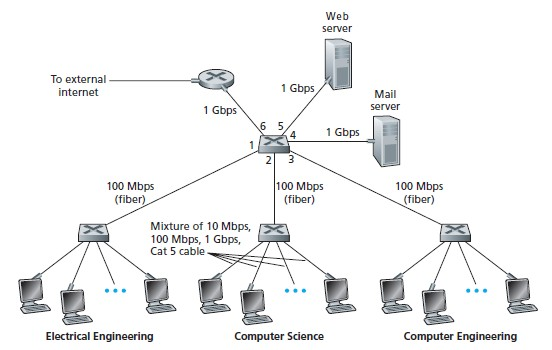
\includegraphics[width=0.95\linewidth]{cap20/switched_lan.png}
\end{minipage}\hfill
\begin{minipage}{0.46\linewidth}
È comune che le LAN usino uno o più switch per collegare molti dispositivi locali (nell'esempio del Kurose, i dipartimenti di un
istituto collegati da switch, con un router verso Internet e i server Web e di posta).
\end{minipage}
\caption{Una rete di istituto con switch organizzati ad albero (da Kurose).}
\end{figure}

A differenza dei router, gli switch sono \textbf{veloci} e \textbf{plug-and-play}:

\begin{itemize}
    \item non c'è alcun algoritmo di routing;
    \item si considerano solo i primi \textbf{2 livelli} della pila.
\end{itemize}

D'altra parte le LAN commutate sono \textbf{limitate in dimensione} e devono essere \textbf{strutturate ad albero}:

\begin{itemize}
    \item gli indirizzi MAC sono difficili da raggruppare (non hanno prefissi legati alla posizione): le tabelle degli switch possono crescere rapidamente;
    \item non c'è routing: i \textbf{cicli} sono difficili da evitare (un frame inondato in un ciclo girerebbe per sempre).
\end{itemize}

\begin{table}[H]
\centering
\begin{tabular}{p{3.5cm}p{5.2cm}p{5.2cm}}
\toprule
 & \textbf{Switch} & \textbf{Router} \\
\midrule
Livello & collegamento (2) & rete (3) \\
Indirizzi & MAC & IP \\
Tabelle & self-learning & algoritmi di routing \\
Configurazione & plug-and-play & va configurato \\
Topologia & albero (niente cicli) & qualsiasi, anche con cicli \\
Traffico broadcast & lo inoltra & lo blocca (separa i domini) \\
\bottomrule
\end{tabular}
\caption{Switch e router a confronto.}
\end{table}

% ══════════════════════════════════════════════════════════════
\section{Il protocollo ARP}
% ══════════════════════════════════════════════════════════════

I protocolli dei livelli superiori lavorano con gli indirizzi IP, mentre il frame ha bisogno dell'indirizzo MAC del destinatario. Serve quindi
tradurre gli indirizzi IP in indirizzi MAC.

\dfn{ARP (Address Resolution Protocol)}{
    L'\textbf{ARP} gestisce la conversione tra indirizzi IP e indirizzi MAC.
    \begin{itemize}
      \item Ogni interfaccia ha un modulo ARP con una \textbf{tabella ARP}, che associa ogni IP della LAN a un indirizzo MAC, con un
            \textbf{TTL} (\emph{time to live}) scaduto il quale la voce viene cancellata (tipicamente 5--20 minuti).
      \item Poiché gli indirizzi MAC sono locali, anche ARP funziona \textbf{solo nelle reti locali}.
    \end{itemize}
}

\begin{table}[H]
\centering
\begin{tabular}{lll}
\toprule
\textbf{Indirizzo IP} & \textbf{Indirizzo MAC} & \textbf{TTL} \\
\midrule
222.222.222.221 & 88-B2-2F-54-1A-0F & 13:45:00 \\
222.222.222.223 & 5C-66-AB-90-75-B1 & 13:52:00 \\
\bottomrule
\end{tabular}
\caption{Una tabella ARP: la voce scade all'orario indicato.}
\end{table}

\info{ARP e DNS}{
    ARP fa per la LAN quello che il DNS fa per Internet: il DNS traduce \textbf{nomi} in indirizzi IP (in tutta Internet), ARP traduce
    \textbf{indirizzi IP} in indirizzi MAC (solo nella propria LAN). Sulle proprie macchine si può vedere la tabella con \texttt{ip neigh}
    (o \texttt{arp -a}).
}

\subsection{Un esempio di ARP}

\begin{figure}[H]
\centering
\begin{minipage}{0.44\linewidth}\centering
  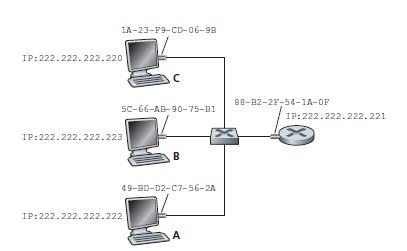
\includegraphics[width=0.95\linewidth]{cap20/arp_lan.png}
\end{minipage}\hfill
\begin{minipage}{0.52\linewidth}
L'host C (\texttt{222.222.222.220}) vuole inviare messaggi all'host A (\texttt{222.222.222.222}). Per farlo deve conoscere anche il MAC di A.
\begin{enumerate}
  \item Se A \textbf{non è nella tabella}, prima di inviare il messaggio C invia in \textbf{broadcast} a tutti i dispositivi della rete un
        pacchetto \textbf{ARP request}: ``chi ha l'IP \texttt{222.222.222.222}? Lo dica a \texttt{222.222.222.220}''.
  \item Tutti i nodi ricevono il pacchetto, ma \textbf{solo} chi ha l'IP cercato risponde, con un messaggio \textbf{ARP reply} diretto
        (\emph{unicast}) che contiene il proprio MAC.
  \item C inserisce la coppia IP--MAC nella propria tabella e invia il frame.
\end{enumerate}
\end{minipage}
\caption{ARP in una LAN: tre host e un router collegati da uno switch (da Kurose).}
\end{figure}

\begin{figure}[H]
\centering
\begin{tikzpicture}[yscale=0.85, every node/.style={font=\scriptsize\sffamily}]
  \timeline{c}{0}{C}{3.6}
  \timeline{b}{4}{B}{3.6}
  \timeline{a}{8}{A}{3.6}
  \draw[msg, netred] (0,-0.5) -- node[above, sloped, pos=0.5] {ARP request (dest. FF-FF-FF-FF-FF-FF): chi ha 222.222.222.222?} (8,-0.5);
  \fill[netred] (4,-0.5) circle (2.5pt); \node[anchor=west, text=netred] at (4.1,-0.85) {riceve e ignora};
  \node[anchor=west] at (8.2,-0.5) {``sono io!''};
  \draw[msg, netgreen!60!black] (8,-1.7) -- node[above, pos=0.5] {ARP reply (unicast): 222.222.222.222 è 49-BD-D2-C7-56-2A} (0,-1.7);
  \node[anchor=east, text width=2.6cm, align=right] at (-0.2,-1.9) {aggiorna la tabella ARP};
  \draw[msg, netblue, very thick] (0,-2.8) -- node[above] {frame IP con MAC di destinazione di A} (8,-2.8);
\end{tikzpicture}
\caption{Richiesta in broadcast, risposta in unicast.}
\end{figure}

\warning{ARP poisoning}{
    ARP non prevede alcuna autenticazione: un host \textbf{malevolo} può intercettare la richiesta e rispondere con una risposta
    \textbf{falsificata}, associando l'IP cercato al proprio MAC (\textbf{ARP poisoning}). I frame destinati alla vittima arrivano così
    all'attaccante, che può leggerli o modificarli (\emph{man in the middle}). È uno degli attacchi più comuni nelle LAN.
}

\subsection{ARP e il gateway}

Che succede se l'IP di destinazione è \textbf{fuori dalla rete}?

\begin{figure}[H]
    \centering
    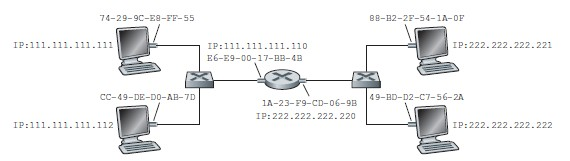
\includegraphics[width=0.7\linewidth]{cap20/arp_gateway.png}
    \caption{Due subnet (111.111.111.x e 222.222.222.x) collegate da un router con due interfacce, ciascuna con il proprio IP, MAC e tabella ARP.}
\end{figure}

\begin{itemize}
    \item Il router che collega le due reti deve avere almeno \textbf{2 interfacce} (2 IP, 2 MAC e 2 tabelle ARP), una dentro ciascuna subnet.
    \item I frame diretti fuori dalla subnet vengono inviati alla \textbf{prima interfaccia del router}: l'host usa ARP per il MAC del
          \textbf{router} (il gateway), non per quello del destinatario finale.
    \item Il router estrae il datagramma, lo sposta sulla seconda interfaccia e, con la seconda tabella ARP, lo invia all'host giusto in un
          \textbf{nuovo frame}.
\end{itemize}

\begin{esempio}{Da A (111.111.111.111) a B (222.222.222.222)}
\begin{enumerate}
    \item A capisce, confrontando indirizzo e maschera, che B è in un'altra subnet: deve passare dal gateway \texttt{111.111.111.110}.
    \item A usa ARP per trovare il MAC dell'interfaccia del router \texttt{111.111.111.110} (\texttt{E6-E9-00-17-BB-4B}).
    \item A crea un datagramma IP con \textbf{IP sorgente A} e \textbf{IP destinazione B}, e lo incapsula in un frame con
          \textbf{MAC destinazione = MAC del router}.
    \item Il router riceve il frame, estrae il datagramma, vede che B è sulla subnet \texttt{222.222.222.0/24}, usa ARP su quell'interfaccia per
          trovare il MAC di B e crea un nuovo frame con \textbf{MAC sorgente = sua seconda interfaccia} e \textbf{MAC destinazione = B}.
\end{enumerate}
\begin{center}
\begin{tabular}{lcccc}
\toprule
\textbf{Tratta} & \textbf{MAC sorgente} & \textbf{MAC destinazione} & \textbf{IP sorgente} & \textbf{IP destinazione} \\
\midrule
A $\rightarrow$ router & A & router (if. 1) & A & B \\
router $\rightarrow$ B & router (if. 2) & B & A & B \\
\bottomrule
\end{tabular}
\end{center}
Gli indirizzi IP restano gli stessi da un estremo all'altro; gli indirizzi MAC cambiano a ogni collegamento.
\end{esempio}

% ══════════════════════════════════════════════════════════════
\section{Il frame Ethernet}
% ══════════════════════════════════════════════════════════════

Ethernet è la tecnologia dominante per le LAN cablate. Nata negli anni '70 come bus condiviso con CSMA/CD, oggi è quasi sempre una
topologia a stella con uno switch al centro e collegamenti full-duplex (dove le collisioni non avvengono più).

\begin{figure}[H]
\centering
\begin{tikzpicture}[every node/.style={font=\scriptsize\sffamily}]
  \node[anchor=east, font=\footnotesize\bfseries\sffamily] at (-0.2,0) {Ethernet (DIX)};
  \node[field, fill=lphy, minimum width=1.6cm] (pr) at (0.8,0) {preambolo};
  \node[field, fill=llink, minimum width=1.9cm, right=0pt of pr] (dst) {indirizzo dest.};
  \node[field, fill=llink, minimum width=1.9cm, right=0pt of dst] (src) {indirizzo sorg.};
  \node[field, fill=lnet!50, minimum width=0.9cm, right=0pt of src] (ty) {tipo};
  \node[field, fill=cloudbg, minimum width=3.2cm, right=0pt of ty] (da) {dati};
  \node[field, fill=cloudbg!50, minimum width=0.9cm, right=0pt of da] (pad) {pad};
  \node[field, fill=netred!25, minimum width=1.3cm, right=0pt of pad] (crc) {CRC};
  \foreach \n/\b in {pr/8, dst/6, src/6, ty/2, da/{0--1500}, pad/{0--46}, crc/4} \node[above=0pt of \n] {\b};
  \node[anchor=east] at (-0.2,0.45) {byte};
  \begin{scope}[yshift=-1.1cm]
    \node[anchor=east, font=\footnotesize\bfseries\sffamily] at (-0.2,0) {IEEE 802.3};
    \node[field, fill=lphy, minimum width=1.3cm] (pr2) at (0.65,0) {preambolo};
    \node[field, fill=lphy!60, minimum width=0.3cm, right=0pt of pr2] (sof) {\rotatebox{90}{\tiny SOF}};
    \node[field, fill=llink, minimum width=1.9cm, right=0pt of sof] (dst2) {indirizzo dest.};
    \node[field, fill=llink, minimum width=1.9cm, right=0pt of dst2] (src2) {indirizzo sorg.};
    \node[field, fill=lnet!50, minimum width=0.9cm, right=0pt of src2] (ln) {lungh.};
    \node[field, fill=cloudbg, minimum width=3.2cm, right=0pt of ln] {dati};
    \node[field, fill=cloudbg!50, minimum width=0.9cm] at (9.95,0) {pad};
    \node[field, fill=netred!25, minimum width=1.3cm] at (11.05,0) {CRC};
  \end{scope}
\end{tikzpicture}
\caption{Il frame Ethernet nelle due varianti (DIX e IEEE 802.3).}
\end{figure}

\begin{itemize}
    \item \textbf{Preambolo} (8 byte): un blocco ``sveglia'' di bit alternati (\texttt{10101010} \dots, con l'ultimo byte \texttt{10101011})
          usato per \textbf{sincronizzare gli orologi} degli adattatori di sorgente e destinazione.
    \item \textbf{Indirizzo di destinazione} (6 byte): il MAC dell'adattatore di destinazione.
    \item \textbf{Indirizzo sorgente} (6 byte): il MAC dell'adattatore che trasmette il frame nella LAN.
    \item \textbf{Tipo} (2 byte): il protocollo di livello di rete contenuto nel frame. Non c'è solo IP (\texttt{0x0800}): per esempio i pacchetti
          ARP hanno un tipo specifico, \texttt{0x0806}. Nella variante 802.3 al suo posto c'è la lunghezza.
    \item \textbf{Dati} (da 46 a 1500 byte): il datagramma IP. Il massimo è la \textbf{MTU} di Ethernet: se il datagramma è più grande, va frammentato.
    \item \textbf{Pad}: riempimento per raggiungere la lunghezza minima dei dati (46 byte), necessaria perché il CSMA/CD rilevi le collisioni
          (tempo di trasmissione di almeno $2\tau$).
    \item \textbf{CRC} (4 byte): il CRC-32 calcolato sul frame, per rilevare gli errori.
\end{itemize}

\info{Un servizio senza connessione e inaffidabile}{
    Ethernet è \textbf{senza connessione} (nessun handshake con l'adattatore di destinazione) e \textbf{inaffidabile}: il ricevente non invia né ACK
    né NAK. Un frame che non supera il controllo CRC viene semplicemente scartato; se i dati servono davvero, sarà TCP (o l'applicazione) a
    accorgersi della mancanza e a ritrasmettere.
}

% ══════════════════════════════════════════════════════════════
\section{Riepilogo}
% ══════════════════════════════════════════════════════════════

\riepilogo{
\begin{itemize}
    \item L'\textbf{indirizzo MAC} (48 bit, esadecimale) identifica un'interfaccia ed è \textbf{locale}; broadcast = \texttt{FF-FF-FF-FF-FF-FF}.
    \item Gli \textbf{switch} inoltrano frame in base al MAC, con tabelle \textbf{self-learning}; sono veloci e plug-and-play ma le LAN commutate
          devono essere ad albero.
    \item \textbf{ARP} traduce IP in MAC: richiesta in broadcast, risposta in unicast, tabella con TTL; vulnerabile all'\textbf{ARP poisoning}.
    \item Verso un'altra subnet il frame va al MAC del \textbf{router}: gli IP restano uguali, i MAC cambiano a ogni hop.
    \item \textbf{Frame Ethernet}: preambolo (8), destinazione (6), sorgente (6), tipo (2), dati (46--1500, con pad), CRC (4).
\end{itemize}
}
  % MAC, switch, ARP, Ethernet

  % ------------------------------------------------------------------
  \part{Sicurezza di rete}
  % ------------------------------------------------------------------
  \chapter{Attacchi alle reti e fondamenti di crittografia}

% ══════════════════════════════════════════════════════════════
\section{Perché la sicurezza di rete}
% ══════════════════════════════════════════════════════════════

Alcune applicazioni scambiano \textbf{informazioni sensibili} (credenziali, dati personali, \dots), e sulle reti pubbliche i messaggi
dovrebbero essere protetti: è il motivo per cui quasi ogni protocollo applicativo ha una variante sicura (HTTPS, SMTPS, SSH, FTPS).

\dfn{Sicurezza di rete}{
    La \textbf{sicurezza di rete} è il campo che studia i possibili \textbf{attacchi} alle reti e i modi per \textbf{prevenirli}.
}

\begin{itemize}
    \item Le reti fanno parte della nostra vita (la connessione a Internet è considerata quasi come l'acqua o la corrente), e una grande
          quantità dei nostri dati sensibili viaggia in rete.
    \item Esistono molti tipi di attacchi, con scopi e meccanismi diversi.
    \item Gli attacchi evolvono insieme alla tecnologia e al pubblico delle reti.
\end{itemize}

% ══════════════════════════════════════════════════════════════
\section{I malware}
% ══════════════════════════════════════════════════════════════

\dfn{Malware}{
    Un \textbf{malware} è un software malevolo che può arrivare su un computer attraverso la rete (un file scaricato, un allegato di posta,
    \dots).
}

Una volta infettato un dispositivo, un malware può fare danni in molti modi:

\begin{table}[H]
\centering
\begin{tabular}{lp{11cm}}
\toprule
\textbf{Tipo} & \textbf{Cosa fa} \\
\midrule
Adware & costringe il sistema a mostrare pubblicità \\
Scareware & mostra falsi allarmi per indurre l'utente a scaricare altri malware \\
Wiper / ransomware & cancella / \textbf{cifra} i file (e chiede un riscatto per restituirli) \\
Spyware & raccoglie informazioni private (password, numeri di documento, \dots); per esempio i \textbf{keylogger} registrano i tasti premuti \\
Rootkit & ottiene i privilegi di amministratore (root) del sistema \\
Zombie / botnet & trasforma il dispositivo in uno ``schiavo'', una testa di ponte per attaccare altri dispositivi \\
\bottomrule
\end{tabular}
\caption{Alcune famiglie di malware.}
\end{table}

I malware di oggi sono spesso \textbf{auto-replicanti}: infettato un host, da lì cercano di entrare in altri host su Internet, e da quelli in
altri ancora. Si diffondono in due forme:

\dfn{Virus e worm}{
    \begin{itemize}
      \item Un \textbf{virus} richiede una qualche \textbf{interazione dell'utente} per infettare il dispositivo. Per esempio un allegato
            con codice eseguibile malevolo che, una volta aperto, si replica inviando mail simili ai contatti dell'utente. I virus sono
            spesso camuffati da componenti software legittimi (\textbf{cavalli di Troia}, \emph{trojan horses}).
      \item Un \textbf{worm} entra in un dispositivo \textbf{senza alcuna interazione} esplicita dell'utente. Per esempio l'utente sta
            eseguendo un'applicazione di rete vulnerabile che accetta il worm senza intervento; il worm poi scansiona la rete alla ricerca
            di altri host con la stessa applicazione.
    \end{itemize}
}

% ══════════════════════════════════════════════════════════════
\section{Gli attacchi DoS}
% ══════════════════════════════════════════════════════════════

\dfn{Denial of Service (DoS)}{
    Gli attacchi \textbf{DoS} (negazione del servizio) sono molto comuni e hanno lo scopo di rendere una rete, un host o un altro pezzo
    di infrastruttura (server Web, DNS, \dots) \textbf{inutilizzabile dagli utenti legittimi}.
}

\begin{figure}[H]
\centering
\begin{minipage}{0.44\linewidth}\centering
  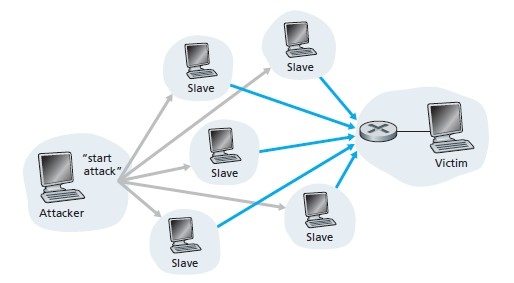
\includegraphics[width=0.95\linewidth]{cap21/ddos.png}
\end{minipage}\hfill
\begin{minipage}{0.52\linewidth}
Ci sono tre tipi di attacchi DoS:
\begin{enumerate}
  \item \textbf{Attacco a una vulnerabilità}: si inviano messaggi costruiti ad arte a un'applicazione o a un sistema operativo vulnerabile
        per bloccarlo o farlo andare in crash.
  \item \textbf{Bandwidth flooding}: si inonda l'host bersaglio di pacchetti, impedendo a quelli legittimi di raggiungerlo.
  \item \textbf{Connection flooding}: si aprono moltissime connessioni TCP, mezze aperte o complete, verso il bersaglio, che smette di
        accettare connessioni legittime (per esempio il \emph{SYN flood}).
\end{enumerate}
\end{minipage}
\caption{Un DDoS (\emph{Distributed DoS}): l'attaccante comanda una botnet di zombie che attaccano la vittima tutti insieme.}
\end{figure}

\info{Perché ``distribuito''}{
    Un solo attaccante ha banda limitata ed è facile da bloccare filtrando il suo indirizzo. Con migliaia di zombie sparsi per il mondo
    il traffico è enorme e proviene da indirizzi diversi, quindi è molto più difficile da distinguere da quello legittimo.
}

% ══════════════════════════════════════════════════════════════
\section{Il packet sniffing}
% ══════════════════════════════════════════════════════════════

\dfn{Packet sniffing}{
    Lo \textbf{sniffing} prevede un ricevitore \textbf{passivo} (lo \emph{sniffer}) che registra una copia dei pacchetti interessanti di un
    host bersaglio, cercando di rubare informazioni sensibili (\emph{eavesdropping}, origliare).
}

\begin{itemize}
    \item Gli sniffer si possono usare in qualunque rete \textbf{broadcast} (cablata o senza fili), semplicemente copiando i pacchetti
          destinati ad altri invece di scartarli.
    \item Nelle reti non broadcast uno sniffer può essere inserito in un malware (spyware) che infetta i dispositivi di rete (per esempio i
          router), in modo che tutto il traffico inoltrato venga anche copiato.
    \item Poiché gli sniffer sono \textbf{passivi} (non immettono traffico nella rete), sono \textbf{difficilissimi da rilevare}.
    \item Per difendersi dallo sniffing si usa la \textbf{crittografia}.
\end{itemize}

Su Internet ci sono molti sniffer liberamente disponibili: un esempio notevole è \textbf{Wireshark} (ex Ethereal), che abbiamo usato nelle
esercitazioni.

% ══════════════════════════════════════════════════════════════
\section{L'IP spoofing}
% ══════════════════════════════════════════════════════════════

\dfn{IP spoofing}{
    L'\textbf{IP spoofing} è la tecnica con cui un host malevolo immette nella rete pacchetti con \textbf{indirizzo sorgente falso}
    (contraffatto).
}

\begin{itemize}
    \item Si può usare, insieme alle vulnerabilità di un'applicazione, per attaccare specifici host fingendosi un altro utente.
    \item Si può usare anche per attacchi DoS (alternativa alle botnet): messaggi da indirizzi sorgente diversi sono più difficili da filtrare.
    \item Spoofing e sniffing insieme permettono attacchi \textbf{man-in-the-middle} (MitM): l'attaccante si mette tra due host che comunicano,
          fingendosi l'uno con l'altro. I due host credono di parlare tra loro, ma in realtà parlano con l'attaccante.
    \item Contro lo spoofing servono controlli di \textbf{integrità dei messaggi} e di \textbf{autenticazione degli estremi}, che permettono di
          stabilire se un messaggio non è stato modificato e se proviene davvero dalla sorgente dichiarata.
\end{itemize}

\begin{figure}[H]
\centering
\begin{tikzpicture}[every node/.style={font=\footnotesize\sffamily}]
  \node (a) at (0,0) {\icon[1cm]{pc}}; \node[below=-2pt of a] {A};
  \node (b) at (9,0) {\icon[1.1cm]{laptop}}; \node[below=-2pt of b] {B};
  \node[draw, fill=netred!20, rounded corners, minimum width=1.4cm, minimum height=0.8cm] (t) at (4.5,-1.2) {T (Trudy)};
  \draw[msg, netred, thick] (a) -- node[above, sloped] {``sono B''} (t);
  \draw[msg, netred, thick] (t) -- node[above, sloped] {``sono A''} (b);
  \draw[dashed, black!40, thick] (a) -- node[above] {A e B credono di parlare direttamente} (b);
\end{tikzpicture}
\caption{L'attacco man-in-the-middle: T finge di essere B con A e di essere A con B, intercettando i messaggi (spesso aiutandosi con lo spoofing).}
\end{figure}

% ══════════════════════════════════════════════════════════════
\section{Le proprietà di una comunicazione sicura}
% ══════════════════════════════════════════════════════════════

Visti i tipi di attacco, possiamo definire le proprietà che una comunicazione sicura dovrebbe garantire.

\dfn{Le quattro proprietà}{
    \begin{itemize}
      \item \textbf{Confidenzialità}: solo il mittente e il destinatario previsto devono poter capire il contenuto del messaggio
            (contro lo \emph{sniffing}).
      \item \textbf{Integrità del messaggio}: il contenuto non deve essere alterato, né in modo malevolo né per errore.
      \item \textbf{Autenticazione degli estremi} (\emph{end-point authentication}): mittente e destinatario devono poter confermare
            l'identità dell'altra parte (contro lo \emph{spoofing}).
      \item \textbf{Sicurezza operativa}: un'infrastruttura di rete che impedisca agli host malevoli di infilarsi nella comunicazione.
    \end{itemize}
}

Le prime tre proprietà sono realizzate \textbf{via software}; l'ultima (sicurezza operativa) si basa tipicamente su \textbf{hardware}
specifico (firewall, sistemi di rilevazione delle intrusioni).

\begin{table}[H]
\centering
\begin{tabular}{lll}
\toprule
\textbf{Attacco} & \textbf{Proprietà violata} & \textbf{Contromisura} \\
\midrule
Sniffing & confidenzialità & crittografia \\
Alterazione dei messaggi & integrità & hash crittografici, MAC \\
Spoofing, replay & autenticazione & nonce, certificati \\
DoS, intrusioni, malware & sicurezza operativa & firewall, IDS \\
\bottomrule
\end{tabular}
\caption{Attacchi, proprietà e contromisure.}
\end{table}

% ══════════════════════════════════════════════════════════════
\section{Introduzione alla crittografia}
% ══════════════════════════════════════════════════════════════

\dfn{Crittografia}{
    Una tecnica \textbf{crittografica} permette a un mittente di \textbf{camuffare i dati} in modo che siano incomprensibili per un intruso:
    l'intruso non deve ricavare alcuna informazione dai dati intercettati, mentre il destinatario deve poter recuperare i dati originali.
    \begin{itemize}
      \item Nella sua forma iniziale il messaggio si chiama \textbf{testo in chiaro} (\emph{plaintext} o \emph{cleartext}) ed è leggibile da tutti.
      \item Prima di immetterlo nel canale, il mittente usa un \textbf{algoritmo di cifratura} che lo trasforma in una forma illeggibile, il
            \textbf{testo cifrato} (\emph{ciphertext}), che va \textbf{decifrato} alla ricezione.
    \end{itemize}
}

\begin{figure}[H]
    \centering
    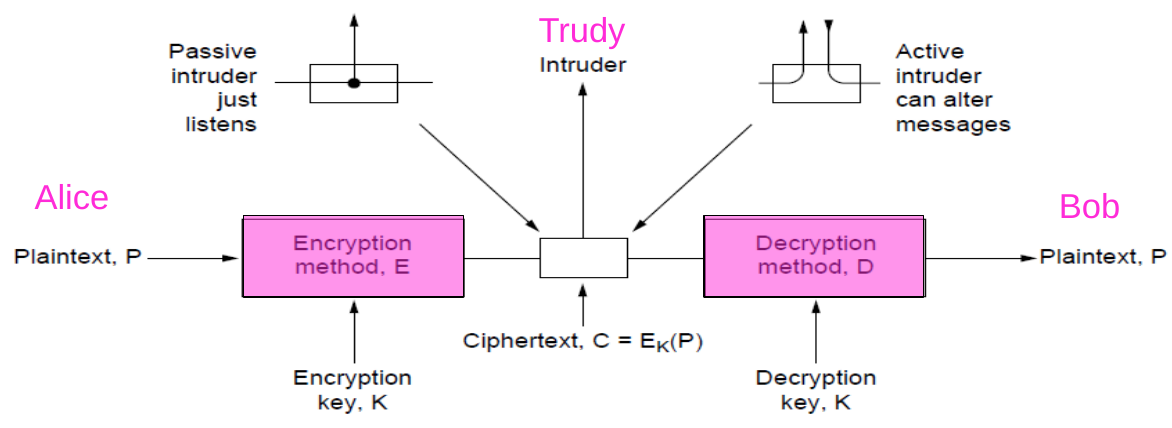
\includegraphics[width=0.72\linewidth]{cap21/modello_intruso.png}
    \caption{Il modello di cifratura (da Tanenbaum): Alice cifra con la chiave $K_E$, Bob decifra con $K_D$; Trudy può ascoltare passivamente o intervenire attivamente.}
\end{figure}

Con la notazione del Tanenbaum:

\begin{itemize}
    \item $K$ è la \textbf{chiave}, $P$ il messaggio in chiaro (\emph{plaintext}), $C$ il messaggio cifrato (\emph{ciphertext});
    \item la cifratura con chiave $K$ si scrive $E_K(P) = C$ e la decifratura $D_K(C) = P$, quindi $D_K(E_K(P)) = P$.
\end{itemize}

\subsection{Le chiavi e il principio di Kerckhoffs}

Nei sistemi crittografici moderni, compresi quelli di Internet, la tecnica di cifratura è \textbf{nota e standard per tutti} (anche per
l'intruso). La parte sconosciuta sono le \textbf{chiavi di cifratura e decifratura}.

\dfn{Chiave}{
    Una \textbf{chiave} è una stringa alfanumerica che va fornita all'algoritmo di cifratura o decifratura per cifrare o decifrare i messaggi.
    Le chiavi di cifratura e decifratura possono essere \textbf{identiche} (crittografia \emph{simmetrica}) o \textbf{diverse}
    (\emph{asimmetrica}).
}

\dfn{Principio di Kerckhoffs}{
    \textbf{Tutti gli algoritmi devono essere pubblici; solo le chiavi sono segrete.} La ``sicurezza per oscurità'' (\emph{security by
    obscurity}), cioè tenere segreto l'algoritmo, non funziona mai: gli algoritmi pubblici vengono studiati e attaccati da migliaia di esperti,
    e quelli che resistono sono davvero robusti.
}

\subsection{I problemi della crittoanalisi}

Chi cerca di ``rompere'' un cifrario (il \emph{crittoanalista}) può trovarsi in tre situazioni, dalla più difficile alla più favorevole:

\begin{enumerate}
    \item \textbf{solo testo cifrato} (\emph{ciphertext only}): ha a disposizione solo testi cifrati;
    \item \textbf{testo in chiaro noto} (\emph{known plaintext}): ha alcuni testi cifrati e i corrispondenti testi in chiaro;
    \item \textbf{testo in chiaro scelto} (\emph{chosen plaintext}): può cifrare a piacere testi in chiaro scelti da lui.
\end{enumerate}

Un buon cifrario deve resistere anche nel terzo caso.

\subsection{Cifrari per sostituzione}

\dfn{Cifrario per sostituzione}{
    In un cifrario per \textbf{sostituzione} ogni simbolo viene sostituito con un altro. La chiave è la \textbf{corrispondenza tra simboli}.
}

\begin{center}
\begin{tabular}{rl}
testo in chiaro: & \texttt{a b c d e f g h i j k l m n o p q r s t u v w x y z} \\
testo cifrato: & \texttt{Q W E R T Y U I O P A S D F G H J K L Z X C V B N M} \\
\end{tabular}
\end{center}

Con questa chiave \texttt{attacco} diventa \texttt{QZZQEEG}. Anche se le chiavi possibili sono $26! \approx 4\cdot 10^{26}$, per l'alfabeto
latino (e altri) questi cifrari sono \textbf{facilmente attaccabili}: si sfruttano le \textbf{regolarità statistiche} della lingua (in italiano
le lettere più frequenti sono e, a, i, o; le doppie sono frequenti; certe coppie di lettere sono comunissime).

\subsection{Cifrari per trasposizione}

\dfn{Cifrario per trasposizione}{
    In un cifrario per \textbf{trasposizione} i simboli \textbf{non cambiano}, ma vengono \textbf{riordinati}. Nel cifrario a trasposizione per
    colonne la chiave è una parola senza lettere ripetute: le sue lettere, in ordine alfabetico, danno l'ordine con cui leggere le colonne.
}

\begin{figure}[H]
    \centering
    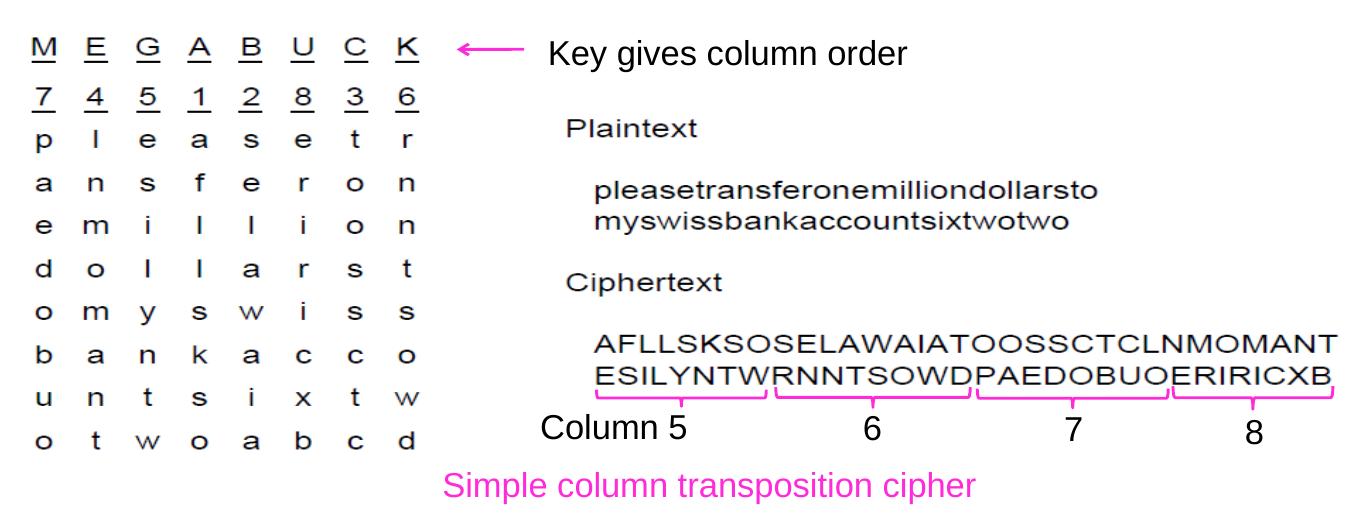
\includegraphics[width=0.55\linewidth]{cap21/trasposizione.png}
    \caption{Trasposizione per colonne con chiave MEGABUCK (da Tanenbaum): il testo si scrive per righe e si legge colonna per colonna, nell'ordine indicato dai numeri.}
\end{figure}

% ══════════════════════════════════════════════════════════════
\section{La crittografia simmetrica}
% ══════════════════════════════════════════════════════════════

\dfn{Crittografia simmetrica}{
    Nella crittografia \textbf{simmetrica} c'è \textbf{una sola chiave}, usata sia per cifrare sia per decifrare.
    \begin{itemize}
      \item \textbf{Cifratura}: il testo in chiaro, insieme alla chiave, viene passato all'algoritmo di cifratura, che genera un testo cifrato
            che può viaggiare in rete in sicurezza.
      \item \textbf{Decifratura}: il testo cifrato, insieme alla chiave, viene passato all'algoritmo di decifratura, che ricrea il testo in chiaro.
    \end{itemize}
}

\begin{figure}[H]
\centering
\begin{tikzpicture}[every node/.style={font=\footnotesize\sffamily}]
  \node[draw, fill=white, rounded corners] (p1) at (0,0) {testo in chiaro};
  \node[draw, fill=netred!20, minimum width=2cm, minimum height=0.8cm] (e) at (3,0) {cifratura};
  \node[draw, fill=lphy!60, rounded corners] (c) at (6.5,0) {testo cifrato};
  \node[draw, fill=netgreen!20, minimum width=2cm, minimum height=0.8cm] (d) at (10,0) {decifratura};
  \node[draw, fill=white, rounded corners] (p2) at (13,0) {testo in chiaro};
  \draw[msg] (p1) -- (e); \draw[msg] (e) -- (c); \draw[msg] (c) -- node[above, text=netred] {canale} (d); \draw[msg] (d) -- (p2);
  \node (k1) at (3,1.3) {chiave $K$};
  \node (k2) at (10,1.3) {stessa chiave $K$};
  \draw[msg] (k1) -- (e); \draw[msg] (k2) -- (d);
  \node[draw, fill=netred!15, rounded corners] (t) at (6.5,-1.3) {intruso};
  \draw[msg, dashed, netred] (c) -- node[right] {sniffing: vede solo il cifrato} (t);
\end{tikzpicture}
\caption{Crittografia simmetrica: la stessa chiave serve a cifrare e a decifrare.}
\end{figure}

\subsection{Il problema dello scambio delle chiavi}

\warning{Come ci si scambia la chiave?}{
    Il problema della crittografia simmetrica (a chiave singola) è che la chiave segreta deve essere \textbf{comunicata} (\emph{key
    exchange problem}).
    \begin{itemize}
      \item Gli host possono usare un \textbf{canale sicuro} per scambiarsi la chiave.
      \item Gli host possono usare un \textbf{protocollo} che permetta loro di ``convergere'' su una chiave condivisa.
    \end{itemize}
    Se due parti non riescono a stabilire in modo sicuro la chiave iniziale, non potranno comunicare in sicurezza: un terzo che abbia
    intercettato la chiave durante lo scambio potrà leggere tutti i messaggi. Inoltre, con $N$ utenti che vogliono parlare a coppie servono
    $\frac{N(N-1)}{2}$ chiavi, una per ogni coppia (dell'ordine di $N^2$).
}

\subsection{Il one-time pad}

\dfn{One-time pad}{
    Il \textbf{one-time pad} è un cifrario \textbf{inviolabile}: si sceglie come chiave (il \emph{pad}) una stringa di bit
    \textbf{casuale}, lunga quanto il messaggio, e si cifra facendo lo XOR bit a bit: $C = P \oplus K$. Per decifrare si rifà lo XOR con lo
    stesso pad: $C \oplus K = P \oplus K \oplus K = P$.
}

\begin{esempio}{Cifrare e decifrare con lo XOR}
Con $P = \texttt{0111}$ e $K = \texttt{1101}$:
\begin{center}
\begin{tabular}{lcl}
cifratura & $P \oplus K$ & $= \texttt{0111} \oplus \texttt{1101} = \texttt{1010} = C$ \\
decifratura & $C \oplus K$ & $= \texttt{1010} \oplus \texttt{1101} = \texttt{0111} = P$ \\
\end{tabular}
\end{center}
\end{esempio}

\begin{figure}[H]
    \centering
    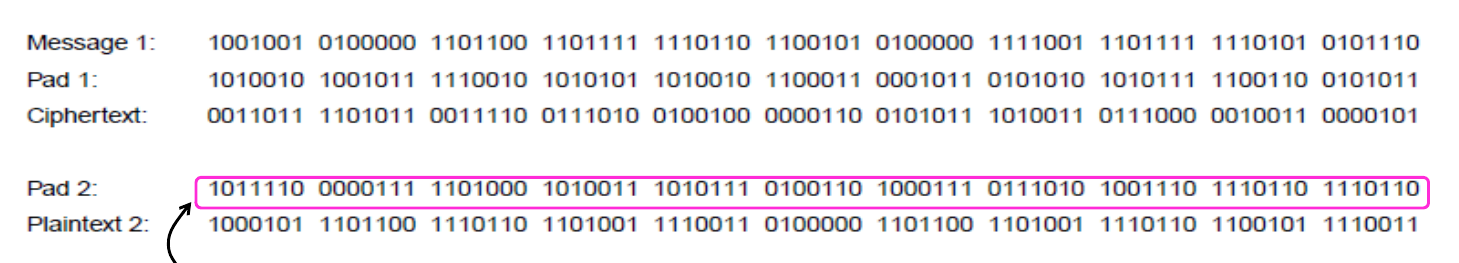
\includegraphics[width=0.82\linewidth]{cap21/one_time_pad.png}
    \caption{Con il one-time pad, dallo stesso testo cifrato si ottengono testi in chiaro diversi usando pad diversi (da Tanenbaum): senza il pad, ogni messaggio della stessa lunghezza è ugualmente probabile.}
\end{figure}

Il one-time pad introduce una grande quantità di ridondanza e impedisce che qualsiasi informazione del testo in chiaro $P$ si rifletta nel
testo cifrato $C$. Ha però problemi pratici:

\begin{enumerate}
    \item \textbf{condivisione del pad}: il pad (la chiave) va distribuito in sicurezza;
    \item \textbf{errori di sincronizzazione}: se il messaggio ha uno spostamento (un bit perso), la decifratura fallisce da lì in poi;
    \item il punto vero: il pad ha la \textbf{stessa dimensione del messaggio}. Se si ha un modo sicuro di trasmettere il pad, tanto vale
          trasmettere direttamente il messaggio (salvo casi particolari, come uno scambio di persona del pad su un supporto fisico).
\end{enumerate}

\warning{One-time vuol dire una volta sola}{
    Un pad \textbf{non deve mai essere usato più di una volta}: se due messaggi sono cifrati con lo stesso pad, $C_1 \oplus C_2 = P_1 \oplus P_2$,
    e da questo l'intruso può ricavare molto sui due testi in chiaro.
}

\subsection{Due principi fondamentali}

\dfn{I due principi della crittografia}{
    \begin{enumerate}
      \item \textbf{Ridondanza}: ogni messaggio cifrato deve contenere una qualche forma di ridondanza. Altrimenti un attaccante potrebbe inviare
            un messaggio cifrato \textbf{a caso}, che dopo la decifratura verrebbe accettato come valido.
      \item \textbf{Freschezza}: serve un meccanismo per prevenire la \textbf{ripetizione} di vecchi messaggi (\emph{replay attack}).
    \end{enumerate}
}

\begin{esempio}{Ridondanza e freschezza in pratica}
\begin{itemize}
    \item \textbf{Ridondanza}: l'attaccante genera un $C$ a caso e lo manda. Se il destinatario accetta qualsiasi $D_K(C)$, lo scambia per un
          messaggio valido. Se invece ogni messaggio contiene anche un campo di controllo (per esempio $h = H(m)$, così che si invia
          $E_K(m, h)$), il destinatario decifra, ricalcola $H(m)$ e verifica la corrispondenza: un $C$ casuale non la supera.
    \item \textbf{Freschezza}: T registra un messaggio cifrato valido da A a B (per esempio ``paga 100 euro a T'') e lo rimanda a B più tardi. B lo
          decifra correttamente e lo esegue di nuovo! Si risolve con i \textbf{timestamp} (messaggi validi solo per poco tempo) o con numeri usati
          una sola volta (\emph{nonce}), che vedremo parlando di autenticazione.
\end{itemize}
\end{esempio}

\subsection{Algoritmi a chiave simmetrica: il DES}

\dfn{DES (Data Encryption Standard)}{
    Il \textbf{DES} è un algoritmo a chiave simmetrica storico:
    \begin{itemize}
      \item il testo in chiaro viene cifrato a \textbf{blocchi di 64 bit};
      \item la cifratura avviene in \textbf{19 stadi};
      \item usa una chiave da \textbf{56 bit} (esistono versioni con chiavi più lunghe, come il Triple DES): la versione a 56 bit oggi
            \textbf{non è più considerata sicura}. Il suo successore è l'\textbf{AES}.
    \end{itemize}
}

\begin{figure}[H]
    \centering
    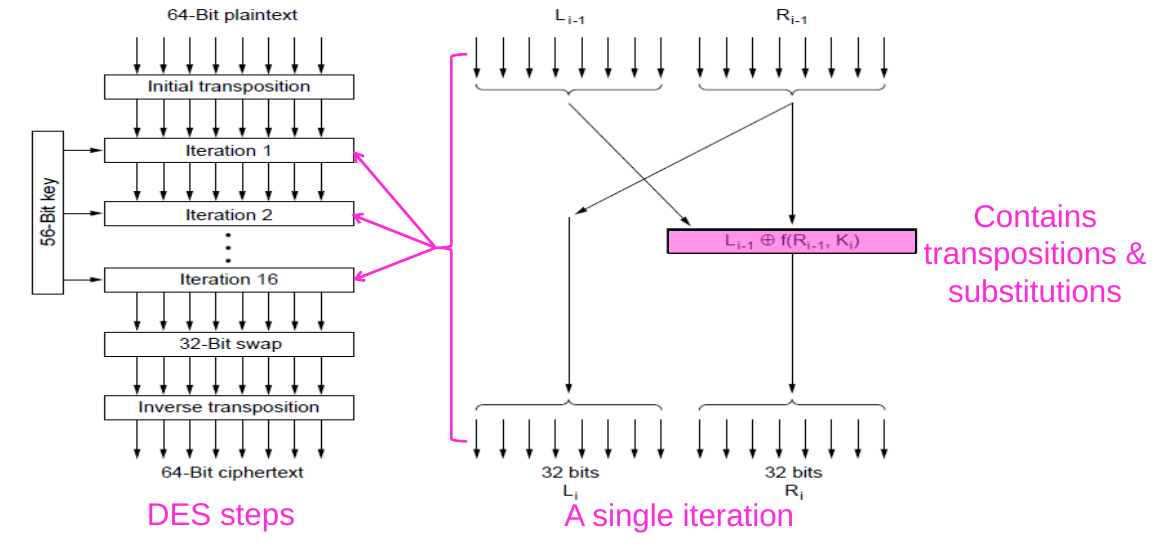
\includegraphics[width=0.62\linewidth]{cap21/des.png}
    \caption{La struttura del DES (da Tanenbaum): a sinistra i 19 stadi, a destra una singola iterazione.}
\end{figure}

\begin{itemize}
    \item Il primo e l'ultimo stadio sono \textbf{trasposizioni} (una inversa dell'altra); il diciottesimo scambia i due blocchi da 32 bit.
    \item Nei 16 stadi intermedi, detti iterazioni: i 32 bit di sinistra dell'uscita sono i 32 bit di destra dell'ingresso ($L_i = R_{i-1}$);
          quelli di destra sono $L_{i-1} \oplus f(R_{i-1}, K_i)$, dove la funzione $f$ \textbf{espande}, fa lo \textbf{XOR con la chiave}
          dell'iterazione $K_i$ e applica \textbf{sostituzioni} e \textbf{trasposizioni}.
    \item La chiave $K_i$ è diversa per ogni iterazione (derivata dalla chiave principale per trasposizione).
\end{itemize}

\subsection{Le modalità di cifratura: il CBC}

\warning{Cifrare blocco per blocco non basta}{
    Il DES eseguito blocco per blocco non è altro che una \textbf{sostituzione} di simboli in altri simboli: ogni blocco da 64 bit viene
    cifrato separatamente, quindi blocchi di testo in chiaro \textbf{uguali} producono blocchi cifrati \textbf{uguali}. Un attaccante potrebbe
    riconoscere schemi ripetuti, o scambiare e ricombinare blocchi (per esempio in una busta paga cifrata, sostituire il blocco dello stipendio
    con quello di un collega più pagato).
}

\dfn{CBC (Cipher Block Chaining)}{
    Il \textbf{CBC} è una modalità di cifratura molto usata che \textbf{concatena} i blocchi con lo XOR:
    $$C_0 = E_K(P_0 \oplus IV), \qquad C_i = E_K(P_i \oplus C_{i-1})$$
    dove $IV$ è un \textbf{vettore di inizializzazione} casuale, diverso per ogni messaggio. Così lo stesso blocco in chiaro produce blocchi
    cifrati diversi a seconda di tutto ciò che lo precede.
}

\begin{figure}[H]
    \centering
    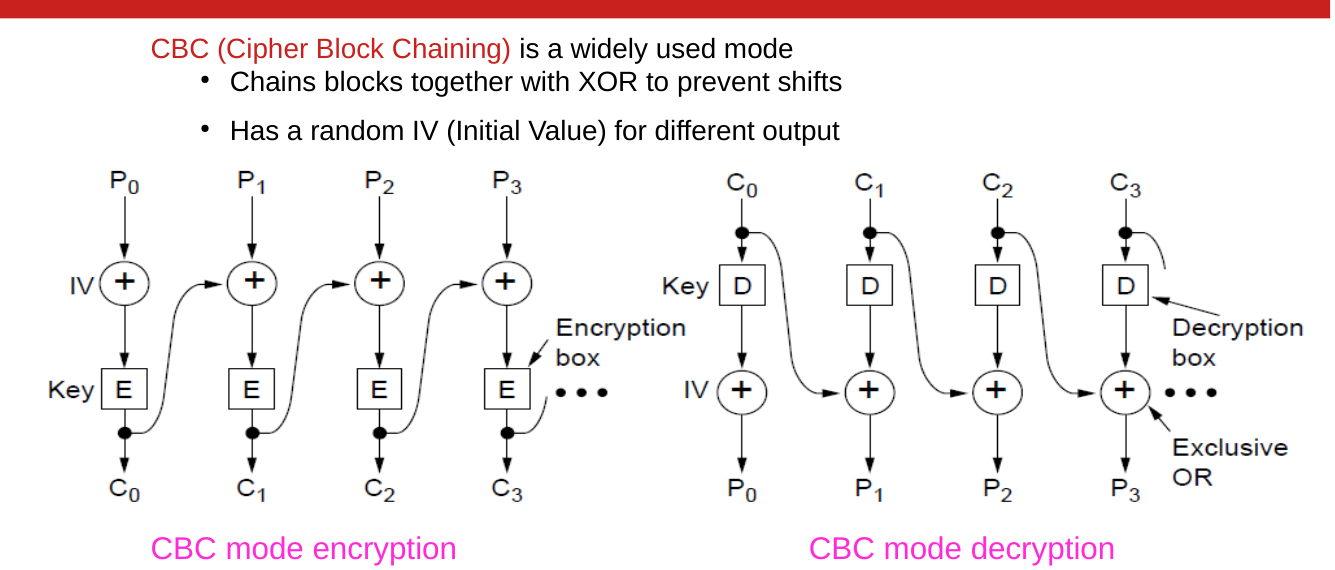
\includegraphics[width=0.75\linewidth]{cap21/cbc.png}
    \caption{CBC: cifratura (a sinistra) e decifratura (a destra), $P_i = D_K(C_i) \oplus C_{i-1}$.}
\end{figure}

% ══════════════════════════════════════════════════════════════
\section{L'integrità dei messaggi}
% ══════════════════════════════════════════════════════════════

\dfn{Integrità del messaggio}{
    L'\textbf{integrità del messaggio} (detta anche \emph{autenticazione del messaggio}) è il problema di verificare che:
    \begin{enumerate}
      \item il messaggio \textbf{non sia stato manomesso};
      \item il messaggio sia stato davvero \textbf{originato dall'host previsto}.
    \end{enumerate}
}

Si può creare un elemento di controllo, in modo simile al checksum o al CRC. Tipicamente si usa una \textbf{funzione hash}, cioè una
funzione che associa a dati di dimensione arbitraria valori di dimensione fissa.

\dfn{Funzione hash crittografica}{
    Una \textbf{funzione hash crittografica} è una funzione $H$ che trasforma un messaggio $x$ in una stringa di dimensione fissa $H(x)$ tale
    che sia \textbf{computazionalmente impossibile} trovare un altro messaggio $y$ con $H(y) = H(x)$. Esempi: SHA-256 (e i vecchi MD5 e SHA-1,
    oggi considerati insicuri).
}

\subsection{Primo tentativo: accodare l'hash}

\begin{enumerate}
    \item A crea il messaggio $m$ e calcola l'hash $h = H(m)$.
    \item A accoda $h$ al messaggio, creando il messaggio esteso $(m, h)$, e lo invia a B.
    \item B riceve $(m, h)$ e calcola $H(m)$. Se $H(m) = h$, il messaggio è integro.
\end{enumerate}

\warning{Un approccio ovviamente difettoso}{
    Un intruso può falsificare l'intero messaggio $(m, h)$, creandone uno nuovo ``su misura'' $(m', h')$ con $h' = H(m')$: è comunque coerente con
    la funzione hash, e B lo accetta. La funzione $H$ è pubblica, quindi chiunque può calcolarla.
}

\subsection{Il MAC: hash con segreto condiviso}

\dfn{Message Authentication Code (MAC)}{
    A e B condividono un \textbf{segreto} $s$ (una chiave o una password), una stringa nota solo a loro.
    \begin{enumerate}
      \item A crea la concatenazione $m + s$ e ne calcola l'hash $h = H(m + s)$: è il \textbf{MAC} (\emph{Message Authentication Code}).
      \item A accoda il MAC al messaggio, creando $(m, H(m+s))$, e lo invia a B.
      \item B riceve $(m, h)$ e, conoscendo $s$, calcola $H(m+s)$. Se coincide con $h$, il messaggio è integro e viene da A.
    \end{enumerate}
    Un intruso che invia $(m', h')$ non conosce $s$: non può calcolare $H(m'+s)$, e B scopre la falsificazione.
}

\begin{figure}[H]
\centering
\begin{tikzpicture}[yscale=0.85, every node/.style={font=\scriptsize\sffamily}]
  \timeline{a}{0}{Host A}{4.2}
  \timeline{t}{4.5}{Intruso}{4.2}
  \timeline{b}{9}{Host B}{4.2}
  \node[draw, fill=llink!50, anchor=east] at (-0.2,-0.5) {$h = H(m + s)$};
  \draw[msg, netblue] (0,-0.8) -- node[above] {$(m, h)$} (4.5,-1.4);
  \node[draw, fill=netred!20] at (4.5,-2.0) {sostituisce};
  \draw[msg, netred] (4.5,-2.6) -- node[above] {$(m', h')$} (9,-3.2);
  \node[draw, fill=netred!10, anchor=west, text width=3cm, align=left] at (9.2,-3.4) {$h' \neq H(m' + s)$: il messaggio è falso!};
\end{tikzpicture}
\caption{Con il segreto condiviso l'intruso non riesce più a costruire un MAC valido.}
\end{figure}

\warning{Un nome, due significati}{
    Qui MAC significa \textbf{Message Authentication Code}, e non ha nulla a che vedere con il \emph{Medium Access Control} (e gli indirizzi MAC)
    del livello di collegamento.
}

Come in tutti gli approcci simmetrici, il segreto va \textbf{scambiato}: lo si può fare combinando crittografia asimmetrica e certificati.

% ══════════════════════════════════════════════════════════════
\section{La crittografia asimmetrica}
% ══════════════════════════════════════════════════════════════

\dfn{Crittografia asimmetrica (a chiave pubblica)}{
    Nella crittografia \textbf{asimmetrica} ci sono \textbf{due chiavi} per ogni partecipante: una \textbf{pubblica} e una \textbf{privata}.
    \begin{itemize}
      \item Un messaggio cifrato con una delle due chiavi va decifrato con l'altra, e viceversa.
      \item La chiave pubblica può essere inviata su canali non sicuri o pubblicata; la chiave privata è disponibile \textbf{solo al proprietario}.
    \end{itemize}
}

\begin{figure}[H]
\centering
\begin{tikzpicture}[every node/.style={font=\footnotesize\sffamily}]
  \node[draw, fill=white, rounded corners] (p1) at (0,0) {testo in chiaro};
  \node[draw, fill=netred!20, minimum width=2cm, minimum height=0.8cm] (e) at (3,0) {cifratura};
  \node[draw, fill=lphy!60, rounded corners] (c) at (6.5,0) {testo cifrato};
  \node[draw, fill=netgreen!20, minimum width=2cm, minimum height=0.8cm] (d) at (10,0) {decifratura};
  \node[draw, fill=white, rounded corners] (p2) at (13,0) {testo in chiaro};
  \draw[msg] (p1) -- (e); \draw[msg] (e) -- (c); \draw[msg] (c) -- (d); \draw[msg] (d) -- (p2);
  \node (k1) at (3,1.3) {chiave \textbf{pubblica} di B};
  \node (k2) at (10,1.3) {chiave \textbf{privata} di B};
  \draw[msg] (k1) -- (e); \draw[msg] (k2) -- (d);
  \node[draw, fill=netred!15, rounded corners, text width=4.5cm, align=center] (t) at (6.5,-1.5) {l'intruso può conoscere la chiave pubblica, ma non può decifrare};
  \draw[msg, dashed, netred] (c) -- (t);
\end{tikzpicture}
\caption{A cifra con la chiave pubblica di B; solo B, con la propria chiave privata, può decifrare.}
\end{figure}

L'uso tipico: cifrare con la \textbf{chiave pubblica} del destinatario e decifrare con la sua \textbf{chiave privata}.

\begin{itemize}
    \item Se l'intruso intercetta la chiave pubblica, non riesce comunque a decifrare i messaggi.
    \item L'host A usa la chiave pubblica di B per cifrare messaggi che si possono leggere solo con la chiave privata di B, che è solo nelle mani di B.
\end{itemize}

\info{Pro e contro rispetto alla crittografia simmetrica}{
    \begin{itemize}
      \item[\itick] La chiave privata \textbf{non va distribuita}; basta una coppia di chiavi per utente (invece di $N^2$ chiavi a coppie).
      \item[\icross] La sicurezza si basa su proprietà matematiche ed è molto \textbf{più lenta} (circa 1000 volte) della crittografia simmetrica.
    \end{itemize}
    Per questo la si usa soprattutto per \textbf{stabilire chiavi simmetriche di sessione}, con cui poi si cifrano i dati.
}

\dfn{Requisiti di un algoritmo a chiave pubblica}{
    \begin{enumerate}
      \item $D(E(P)) = P$ (correttezza);
      \item deve essere estremamente difficile ricavare la chiave privata da quella pubblica;
      \item $E$ non deve poter essere violato con un attacco a \textbf{testo in chiaro scelto}: l'intruso ha la chiave pubblica, quindi può cifrare
            tutti i testi in chiaro che vuole.
    \end{enumerate}
}

\subsection{RSA}

\dfn{RSA}{
    L'\textbf{RSA} (Rivest, Shamir, Adleman) è l'algoritmo a chiave pubblica più diffuso. La sua sicurezza si basa sulla difficoltà di
    \textbf{fattorizzare numeri grandi}.
    \begin{itemize}
      \item \textbf{Generazione delle chiavi}: si scelgono due numeri primi grandi $p$ e $q$; si calcolano $n = p \cdot q$ e $z = (p-1)(q-1)$; si
            sceglie $d$ primo con $z$; si trova $e$ tale che $e \cdot d \equiv 1 \pmod z$. La chiave \textbf{pubblica} è $(e, n)$, quella
            \textbf{privata} è $(d, n)$.
      \item \textbf{Cifratura} (per un messaggio di $k$ bit, visto come numero $P < n$): $C = P^e \bmod n$.
      \item \textbf{Decifratura}: $P = C^d \bmod n$.
    \end{itemize}
}

\begin{esempio}{RSA con numeri piccoli (da Tanenbaum)}
$p = 3$, $q = 11$: $n = 33$, $z = 2 \cdot 10 = 20$. Scegliamo $d = 7$ (primo con 20) e cerchiamo $e$ con $7e \equiv 1 \pmod{20}$: $e = 3$
($21 \bmod 20 = 1$). Chiave pubblica $(3, 33)$, privata $(7, 33)$.
\begin{itemize}
    \item Cifrare $P = 19$: $C = 19^3 \bmod 33 = 6859 \bmod 33 = 28$.
    \item Decifrare: $P = 28^7 \bmod 33 = 19$.
\end{itemize}
Con numeri di centinaia di cifre, ricavare $d$ da $(e, n)$ richiederebbe di fattorizzare $n$: praticamente impossibile.
\end{esempio}

\subsection{Lo scambio di chiavi Diffie-Hellman}

\dfn{Diffie-Hellman}{
    Il protocollo \textbf{Diffie-Hellman} permette a due parti di stabilire un \textbf{segreto condiviso} su un canale pubblico.
    \begin{enumerate}
      \item Alice sceglie un numero segreto $x$ e invia a Bob due numeri pubblici $n$ e $g$ (primi grandi) e il valore $g^x \bmod n$.
      \item Bob sceglie un numero segreto $y$ e invia ad Alice $g^y \bmod n$.
      \item Alice calcola $(g^y \bmod n)^x \bmod n = g^{xy} \bmod n$; Bob calcola $(g^x \bmod n)^y \bmod n = g^{xy} \bmod n$.
    \end{enumerate}
    Entrambi ottengono lo stesso segreto $g^{xy} \bmod n$. Un intruso che ascolta conosce $n$, $g$, $g^x \bmod n$ e $g^y \bmod n$, ma non può
    calcolare $g^{xy} \bmod n$ senza conoscere $x$ o $y$: ricavarli dalle potenze modulari (il \emph{logaritmo discreto}) è praticamente
    impossibile.
}

\begin{figure}[H]
    \centering
    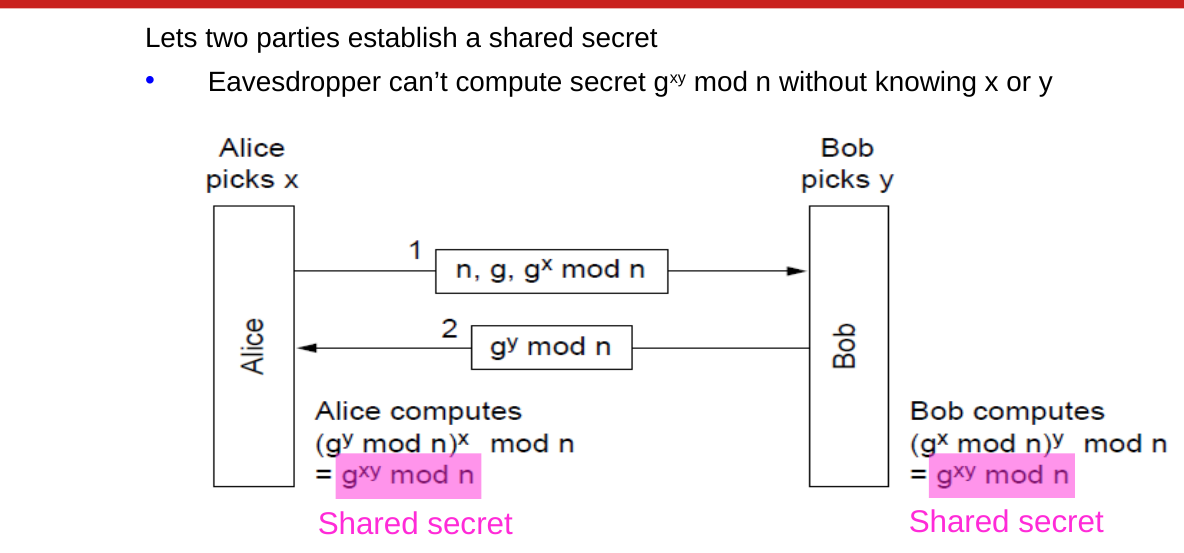
\includegraphics[width=0.52\linewidth]{cap21/dh.png}
    \caption{Lo scambio di chiavi Diffie-Hellman.}
\end{figure}

\warning{L'attacco man-in-the-middle a Diffie-Hellman}{
    Diffie-Hellman da solo è vulnerabile a un attacco \textbf{man-in-the-middle}: Trudy intercetta $g^x \bmod n$ di Alice e le risponde con un proprio
    $g^z \bmod n$, poi fa lo stesso con Bob. Alice crede di condividere un segreto con Bob, ma lo condivide con Trudy ($g^{xz}$), e così Bob
    ($g^{yz}$). Trudy decifra, legge e ricifra tutto. Serve \textbf{confermare le identità}, non solo condividere un segreto: è il ruolo dei
    certificati.
    \begin{center}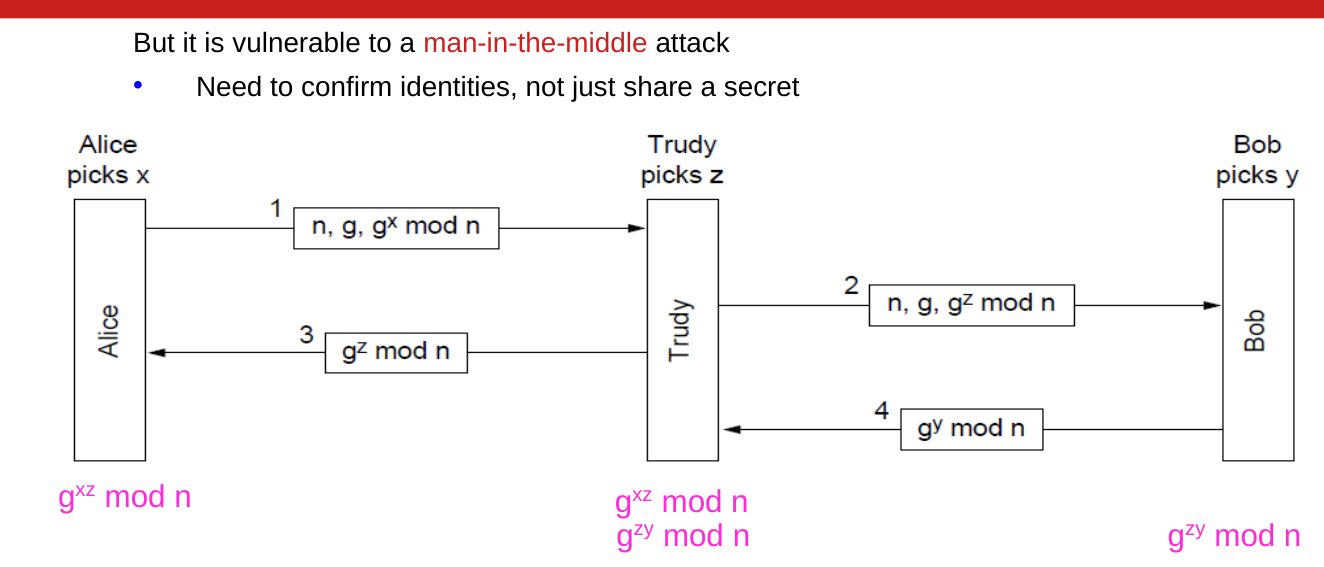
\includegraphics[width=0.55\linewidth]{cap21/dh_attacco.png}\end{center}
}

% ══════════════════════════════════════════════════════════════
\section{Le autorità di certificazione}
% ══════════════════════════════════════════════════════════════

Con la crittografia a chiave pubblica è fondamentale verificare che una chiave pubblica appartenga davvero all'entità con cui si vuole
comunicare. Altrimenti potremmo avere la chiave di qualcun altro (un attaccante) e cifrare messaggi leggibili da estranei.

\dfn{Autorità di certificazione (CA)}{
    Il legame tra una chiave pubblica e una certa entità viene tipicamente certificato da una \textbf{Certification Authority} (CA), il cui
    compito è validare le identità ed emettere certificati.
    \begin{enumerate}
      \item Una CA \textbf{verifica che un'entità sia chi dice di essere}. Non esiste un protocollo per farlo: bisogna fidarsi che la CA abbia
            eseguito una verifica sufficientemente rigorosa. Funziona come una selezione naturale: se una CA è inaffidabile nessuno si fida di
            lei; esistono CA pubbliche e statali ragionevolmente affidabili, ma bisogna comunque fidarsi.
      \item Verificata l'identità, la CA crea un \textbf{certificato} che lega la chiave pubblica dell'entità alla sua identità. Il certificato
            contiene la chiave pubblica e un identificativo univoco del proprietario (per esempio un nome o un indirizzo IP), ed è
            \textbf{firmato} digitalmente dalla CA.
    \end{enumerate}
}

\begin{figure}[H]
\centering
\begin{tikzpicture}[every node/.style={font=\footnotesize\sffamily}]
  \node[draw, fill=cloudbg, rounded corners, minimum width=2.6cm, minimum height=1cm] (bob) at (0,0) {Bob: chiave pubblica $K_B^+$ + prova d'identità};
  \node[draw, fill=netgreen!20, rounded corners, minimum width=2.2cm, minimum height=1cm, align=center] (ca) at (6,0) {CA\\(cifra con la propria\\chiave privata)};
  \node[draw, fill=llink!60, rounded corners, text width=3.2cm, align=center] (cert) at (11,0) {\textbf{certificato}: ``$K_B^+$ appartiene a Bob'', firmato dalla CA};
  \draw[msg] (bob) -- (ca); \draw[msg] (ca) -- (cert);
  \node[text width=12cm, align=center] at (6,-1.3) {Alice verifica la firma con la chiave pubblica della CA (già presente nel browser o nel sistema operativo): se è valida, può fidarsi che $K_B^+$ sia di Bob.};
\end{tikzpicture}
\caption{La CA lega una chiave pubblica a un'identità.}
\end{figure}

% ══════════════════════════════════════════════════════════════
\section{Riepilogo}
% ══════════════════════════════════════════════════════════════

\riepilogo{
\begin{itemize}
    \item Attacchi: \textbf{malware} (virus, worm, trojan, ransomware, botnet), \textbf{DoS}/DDoS, \textbf{sniffing} (passivo), \textbf{IP spoofing},
          man-in-the-middle.
    \item Proprietà: \textbf{confidenzialità}, \textbf{integrità}, \textbf{autenticazione}, \textbf{sicurezza operativa}.
    \item \textbf{Kerckhoffs}: algoritmi pubblici, chiavi segrete. Cifrari per sostituzione e trasposizione; one-time pad inviolabile ma impraticabile.
    \item \textbf{Simmetrica} (DES, AES; modalità CBC): una chiave, veloce, ma va scambiata. \textbf{Asimmetrica} (RSA): chiave pubblica e privata,
          lenta, usata per scambiare chiavi. \textbf{Diffie-Hellman}: segreto condiviso, ma vulnerabile al MitM.
    \item \textbf{Integrità}: hash crittografici; il \textbf{MAC} $H(m+s)$ usa un segreto condiviso. Principi: ridondanza e freschezza.
    \item Le \textbf{CA} certificano il legame tra chiave pubblica e identità.
\end{itemize}
}
     % Attacchi e crittografia
  \chapter{Autenticazione, SSL/TLS e sicurezza operativa}

Ricordiamo le quattro proprietà di una comunicazione sicura: \textbf{confidenzialità} (contro lo sniffing), \textbf{integrità del
messaggio}, \textbf{autenticazione degli estremi} (contro lo spoofing) e \textbf{sicurezza operativa}. Le prime tre sono realizzate via
software; l'ultima si basa tipicamente su hardware dedicato. In questo capitolo completiamo l'autenticazione, vediamo come tutto si
combina in SSL/TLS e chiudiamo con firewall e IDS.

% ══════════════════════════════════════════════════════════════
\section{L'autenticazione degli estremi}
% ══════════════════════════════════════════════════════════════

\dfn{Autenticazione degli estremi}{
    L'\textbf{autenticazione degli estremi} (\emph{end-point authentication}) è il processo con cui un'entità \textbf{dimostra la propria
    identità} a un'altra entità attraverso una rete.
}

\begin{itemize}
    \item Tipicamente un \textbf{protocollo di autenticazione} (AP, \emph{Authentication Protocol}) viene eseguito \textbf{prima} che le due
          parti eseguano qualche altro protocollo: serve a stabilire le identità di entrambe prima di cominciare a lavorare.
    \item Esempi di protocolli che ne hanno bisogno: un trasferimento affidabile (basato su TCP), uno scambio di informazioni di routing (DV o
          LS), un protocollo di posta (SMTP), \dots
    \item Per l'autenticazione ci si può appoggiare alle \textbf{CA} viste nel capitolo precedente, ma non basta.
\end{itemize}

% ══════════════════════════════════════════════════════════════
\section{Tentativi progressivi di autenticazione}
% ══════════════════════════════════════════════════════════════

Supponiamo che l'host A debba autenticarsi presso B prima di lavorare insieme. Costruiamo un protocollo per tentativi, correggendo a ogni
passo il difetto del precedente (l'approccio del Kurose, con i protocolli ap1.0, ap2.0, \dots).

\subsection{Tentativo 1: controllare l'indirizzo IP}

Se A e B hanno già comunicato e l'indirizzo IP di A è sempre lo stesso, B potrebbe autenticare A \textbf{controllando l'indirizzo IP} nel
datagramma: se è quello noto, si assume che a inviare sia A.

\warning{Basta falsificare l'indirizzo}{
    Questa tecnica funziona contro intrusi ``ingenui'' che cercano di spacciarsi per A, ma non basta: un intruso ``meno ingenuo'' può
    \textbf{falsificare l'indirizzo} nel pacchetto (spoofing).
}

Un modo di evitare lo spoofing è sfruttare i \textbf{router}: un router può essere configurato per inoltrare solo datagrammi legittimi, cioè con
indirizzo sorgente che appartiene davvero agli host dietro di lui.

\begin{itemize}
    \item Il router deve conoscere gli IP dei propri host (altrimenti gli host sarebbero irraggiungibili).
    \item Può quindi rilevare i pacchetti il cui indirizzo non è coerente con la sorgente, e scartarli prima che facciano danni.
\end{itemize}

Purtroppo questa capacità \textbf{non è universalmente adottata} né imposta: bisogna assumere che lo spoofing sia possibile.

\subsection{Tentativo 2: una password segreta}

Un altro approccio, il più comune, è usare una \textbf{password segreta}: la password funziona come un segreto condiviso tra chi autentica e chi
viene autenticato. Gmail, Facebook, Telnet, FTP e moltissimi altri servizi usano l'autenticazione con password. Lo stesso segreto può servire
anche al controllo di integrità.

\warning{La password si può intercettare}{
    Il primo problema è che l'intruso può \textbf{intercettare la password} (eavesdropping) dai messaggi, e usarla insieme a un IP falsificato. Con
    Telnet, che trasmette tutto in chiaro, basta uno sniffer.
}

\subsection{Tentativo 3: una password cifrata}

L'intercettazione si evita \textbf{cifrando la password}, così che diventi illeggibile per l'intruso. Se si usa una cifratura simmetrica non serve
nemmeno una password aggiuntiva: la chiave condivisa stessa, che deve essere un segreto tra i due host, può fare da password.

\warning{L'attacco a ripetizione (playback)}{
    La cifratura è una buona cosa, ma non basta: un intruso ``molto furbo'' può infilarsi nella comunicazione fingendosi A con un
    \textbf{attacco a ripetizione} (\emph{playback} o \emph{replay attack}).
    \begin{itemize}
      \item L'intruso sniffa i pacchetti da A a B cercando di ottenere la versione \textbf{cifrata} della password di A.
      \item Se ci riesce, può \textbf{ripetere} la password cifrata a B in una nuova sessione, usandola \textbf{senza nemmeno capirla}.
      \item A differenza dei MitM classici (in tempo reale), sniffing e ripetizione avvengono in momenti separati.
    \end{itemize}
    Il problema è che B non riesce a capire se A è ``\textbf{vivo}'', cioè se c'è una sessione attiva in corso tra il vero A e B.
}

\begin{figure}[H]
\centering
\begin{tikzpicture}[yscale=0.8, every node/.style={font=\scriptsize\sffamily}]
  \timeline{a}{0}{A}{4.5}
  \timeline{t}{4}{Trudy}{4.5}
  \timeline{b}{8}{B}{4.5}
  \draw[msg, netblue] (0,-0.4) -- node[above, pos=0.3] {``sono A'', $K_{AB}$(password)} (8,-0.4);
  \fill[netred] (4,-0.4) circle (2.5pt); \node[text=netred, anchor=west] at (4.1,-0.8) {registra};
  \node[text=black!50] at (4,-1.6) {\dots giorni dopo \dots};
  \draw[msg, netred] (4,-2.6) -- node[above] {``sono A'', $K_{AB}$(password)} (8,-2.6);
  \node[anchor=west, text width=2.8cm, align=left] at (8.2,-2.6) {B decifra: la password è corretta!};
\end{tikzpicture}
\caption{L'attacco playback: Trudy non conosce la password, ma riusa il messaggio cifrato.}
\end{figure}

Il problema somiglia all'apertura di una connessione TCP, in cui con il three-way handshake i due host si assicurano di essere entrambi vivi. Nel
three-way handshake gli host usano \textbf{numeri di sequenza iniziali casuali}, perché ritrasmissioni di vecchie connessioni non vengano
scambiate per SYN o SYNACK nuovi. Un'idea simile si può usare per l'autenticazione.

% ══════════════════════════════════════════════════════════════
\section{La soluzione: il nonce}
% ══════════════════════════════════════════════════════════════

\dfn{Nonce}{
    Un \textbf{nonce} è un numero casuale (o pseudocasuale) che un protocollo usa \textbf{una sola volta nella vita} (\emph{number used once}).
}

\begin{figure}[H]
\centering
\begin{tikzpicture}[yscale=0.85, every node/.style={font=\scriptsize\sffamily}]
  \timeline{a}{0}{Host A}{4.6}
  \timeline{b}{7}{Host B}{4.6}
  \node[anchor=east] at (-0.2,-0.2) {chiave $K_{AB}$}; \node[anchor=west] at (7.2,-0.2) {chiave $K_{AB}$};
  \draw[msg] (0,-0.5) -- node[above] {1. ``sono A''} (7,-1.0);
  \node[draw, fill=llink!60, anchor=west] at (7.2,-1.3) {2. crea un nonce $R$ usato una sola volta};
  \draw[msg, netorange] (7,-1.6) -- node[above] {$R$} (0,-2.1);
  \draw[msg, netblue] (0,-2.6) -- node[above] {3. $K_{AB}(R + \text{password})$} (7,-3.1);
  \node[draw, fill=netgreen!20, anchor=west, text width=3.6cm, align=left] at (7.2,-3.6) {4. decifra: se il nonce è quello inviato, dall'altra parte c'è davvero A};
\end{tikzpicture}
\caption{Autenticazione con nonce e chiave simmetrica condivisa.}
\end{figure}

Supponendo che A e B condividano una chiave simmetrica, il nonce si usa così:

\begin{enumerate}
    \item A invia a B il messaggio ``sono A''.
    \item B sceglie un nonce $R$ e lo invia ad A.
    \item A cifra il nonce insieme alla password con la chiave simmetrica condivisa e rimanda il risultato a B.
    \item B decifra il messaggio: se il nonce decifrato coincide con quello che aveva inviato, A è autenticato.
\end{enumerate}

\begin{itemize}
    \item La password diventa una sorta di \textbf{password monouso}: ogni password cifrata è legata al proprio nonce, e non può essere riusata in altre
          sessioni (da qualcun altro).
    \item Se password e nonce arrivano correttamente a B, si può ragionevolmente assumere che dietro ci sia A, \textbf{vivo} in quel momento.
\end{itemize}

\info{Con la crittografia asimmetrica}{
    Lo stesso schema funziona con le chiavi pubbliche: B invia il nonce $R$, A lo cifra con la propria \textbf{chiave privata}, e B lo decifra con la
    chiave \textbf{pubblica} di A. Solo A può aver prodotto quel messaggio. Resta però il problema di essere sicuri che la chiave pubblica sia davvero
    di A: di nuovo servono i \textbf{certificati}.
}

% ══════════════════════════════════════════════════════════════
\section{SSL e TLS}
% ══════════════════════════════════════════════════════════════

Abbiamo visto che diverse tecniche crittografiche si possono usare e integrare per offrire confidenzialità, integrità e autenticazione alle
connessioni TCP.

\dfn{SSL/TLS}{
    Queste tecniche sono realizzate dal \textbf{Secure Socket Layer} (SSL), una versione ``potenziata'' di TCP che offre servizi di sicurezza.
    \begin{itemize}
      \item Una versione leggermente modificata di SSL 3 si chiama \textbf{Transport Layer Security} (TLS), ed è quella usata oggi.
      \item Esiste un equivalente per le comunicazioni basate su UDP, il \textbf{Datagram TLS} (DTLS).
    \end{itemize}
}

\begin{itemize}
    \item SSL è usato da molti protocolli applicativi: Web, posta, messaggistica istantanea, voice over IP, \dots
    \item Spesso la connessione tra il browser e un sito usa \textbf{HTTPS} (HTTP + SSL/TLS) invece di HTTP: il lucchetto nella barra degli indirizzi.
\end{itemize}

\begin{figure}[H]
\centering
\begin{tikzpicture}[every node/.style={font=\footnotesize\sffamily}]
  \begin{scope}
    \node[font=\bfseries\sffamily] at (0,2.3) {TCP normale};
    \node[lay app, minimum width=3cm] (a1) at (0,1.5) {Applicazione};
    \node[lay tra, minimum width=3cm] (t1) at (0,0.6) {TCP};
    \node[lay net, minimum width=3cm] (n1) at (0,-0.3) {IP};
    \node[lay link, minimum width=3cm] (l1) at (0,-1.2) {Accesso (link + fisico)};
    \draw[very thick, netblue] (-1.6,1.05) -- (1.6,1.05); \node[right, text=netblue] at (1.6,1.05) {socket TCP};
  \end{scope}
  \begin{scope}[xshift=7.5cm]
    \node[font=\bfseries\sffamily] at (0,2.3) {TCP con SSL};
    \node[lay app, minimum width=3cm] (a2) at (0,1.8) {Applicazione};
    \node[layer, fill=netred!30, minimum width=3cm] (s2) at (0,1.0) {sottolivello SSL};
    \node[lay tra, minimum width=3cm] (t2) at (0,0.2) {TCP};
    \node[lay net, minimum width=3cm] (n2) at (0,-0.6) {IP};
    \node[lay link, minimum width=3cm] (l2) at (0,-1.4) {Accesso (link + fisico)};
    \draw[very thick, netred] (-1.6,1.4) -- (1.6,1.4); \node[right, text=netred] at (1.6,1.4) {socket SSL};
    \draw[very thick, netblue] (-1.6,0.6) -- (1.6,0.6); \node[right, text=netblue] at (1.6,0.6) {socket TCP};
    \draw[decorate, decoration={brace, amplitude=5pt, mirror}] (-1.7,2.1) -- (-1.7,0.7) node[midway, left=6pt, align=right] {livello\\applicativo};
  \end{scope}
\end{tikzpicture}
\caption{SSL si inserisce tra l'applicazione e TCP: tecnicamente sta nel livello applicativo, ma allo sviluppatore appare come un trasporto sicuro.}
\end{figure}

\begin{itemize}
    \item Poiché SSL protegge TCP, può essere usato da \textbf{qualsiasi applicazione} che gira su TCP.
    \item SSL offre un'\textbf{API} semplice, con socket simili a quelli di TCP: un'applicazione che vuole usare SSL include le librerie SSL.
    \item Anche se SSL risiede tecnicamente nel livello applicativo, dal punto di vista dello sviluppatore sembra un protocollo di trasporto che offre i
          servizi di TCP arricchiti di sicurezza.
\end{itemize}

SSL ha tre fasi principali: \textbf{handshake}, \textbf{derivazione delle chiavi} e \textbf{trasferimento dati}.

% ══════════════════════════════════════════════════════════════
\section{SSL: l'handshake}
% ══════════════════════════════════════════════════════════════

Un client B vuole usare SSL per comunicare con un server A. Nella fase di handshake B deve:

\begin{itemize}
    \item \textbf{stabilire una connessione TCP} con A;
    \item \textbf{verificare che A sia davvero A} (e non un server fasullo);
    \item \textbf{inviare ad A una chiave segreta principale} (\emph{master secret}), il segreto condiviso.
\end{itemize}

\begin{figure}[H]
\centering
\begin{tikzpicture}[yscale=0.72, every node/.style={font=\scriptsize\sffamily}]
  \timeline{b}{0}{Client B}{8.4}
  \timeline{a}{7}{Server A}{8.4}
  \draw[msg, black!60] (0,-0.3) -- node[above] {TCP SYN} (7,-0.8);
  \draw[msg, black!60] (7,-1.0) -- node[above] {TCP SYNACK} (0,-1.5);
  \draw[msg, black!60] (0,-1.7) -- node[above] {TCP ACK} (7,-2.2);
  \draw[msg, netblue, thick] (0,-2.8) -- node[above] {SSL hello} (7,-3.3);
  \draw[msg, netgreen!60!black, thick] (7,-3.6) -- node[above] {certificato (con la chiave pubblica di A)} (0,-4.1);
  \node[draw, fill=llink!60, anchor=east, text width=2.8cm, align=right] at (-0.2,-4.8) {verifica il certificato con la CA; crea il Master Secret MS};
  \draw[msg, netred, thick] (0,-5.6) -- node[above] {$K_A^+$(MS): MS cifrato con la chiave pubblica di A} (7,-6.1);
  \node[draw, fill=llink!60, anchor=west, text width=2.8cm, align=left] at (7.2,-6.5) {decifra con la chiave privata e ottiene MS};
  \node[draw, fill=netgreen!20, text width=5cm, align=center] at (3.5,-7.6) {ora solo A e B conoscono MS};
\end{tikzpicture}
\caption{L'handshake SSL (semplificato).}
\end{figure}

\begin{enumerate}
    \item Stabilita la connessione TCP, B invia ad A un messaggio \textbf{hello}.
    \item Il server A risponde con il proprio \textbf{certificato}, che contiene la sua \textbf{chiave pubblica}.
    \item Poiché il certificato è stato certificato da una CA, il client B si fida che la chiave pubblica nel certificato appartenga ad A.
    \item B genera un \textbf{Master Secret} (MS), che userà solo per questa sessione SSL (è un nonce), lo cifra con la chiave pubblica di A e lo invia ad A.
    \item Il server A decifra il messaggio con la propria chiave privata e ottiene MS. Dopo questa fase, \textbf{solo B e A} conoscono il master secret della sessione.
\end{enumerate}

\info{Asimmetrica per iniziare, simmetrica per lavorare}{
    SSL usa la crittografia \textbf{asimmetrica} (lenta) solo per scambiare in sicurezza il segreto, e poi la crittografia \textbf{simmetrica} (veloce) per
    tutti i dati. È lo schema ibrido tipico di quasi tutti i protocolli sicuri.
}

% ══════════════════════════════════════════════════════════════
\section{SSL: la derivazione delle chiavi}
% ══════════════════════════════════════════════════════════════

Poiché MS è un segreto condiviso tra B e A, potrebbe essere usato come chiave simmetrica per tutta la cifratura e il controllo di integrità della
sessione. È però più sicuro che A e B usino \textbf{chiavi diverse} per la cifratura e per l'integrità, e per i due flussi di dati (da A a B e da B ad A).

Da MS si ricavano \textbf{quattro chiavi}:

\begin{table}[H]
\centering
\begin{tabular}{ll}
\toprule
\textbf{Chiave} & \textbf{Uso} \\
\midrule
$E_{B\rightarrow A}$ & chiave di \textbf{cifratura} di sessione per i dati da B ad A \\
$M_{B\rightarrow A}$ & chiave \textbf{MAC} di sessione per i dati da B ad A \\
$E_{A\rightarrow B}$ & chiave di \textbf{cifratura} di sessione per i dati da A a B \\
$M_{A\rightarrow B}$ & chiave \textbf{MAC} di sessione per i dati da A a B \\
\bottomrule
\end{tabular}
\caption{Le quattro chiavi di sessione derivate dal master secret (MAC = Message Authentication Code).}
\end{table}

% ══════════════════════════════════════════════════════════════
\section{SSL: il trasferimento dati}
% ══════════════════════════════════════════════════════════════

SSL protegge TCP spezzando il flusso di dati dell'applicazione in \textbf{record}. Per ciascun record:

\begin{enumerate}
    \item SSL accoda al record un \textbf{MAC}, per il controllo di integrità ($\text{record}_i + \text{MAC}$);
    \item il record così modificato viene \textbf{cifrato};
    \item il record cifrato viene passato a TCP per la trasmissione.
\end{enumerate}

\warning{E l'integrità dell'intero flusso?}{
    Così si garantisce l'integrità dei singoli record, ma non dell'intero flusso. Poiché è cifrato solo il payload, un MitM tra A e B può ancora
    danneggiare il flusso \textbf{invertendo o eliminando segmenti}. Per esempio può catturare due segmenti consecutivi, scambiarne l'ordine insieme ai
    numeri di sequenza TCP, e inviarli al ricevente, che non si accorge dell'inversione finché i dati non arrivano all'applicazione.
}

Per evitarlo SSL integra anche un \textbf{numero di sequenza} nel messaggio prima della cifratura: il vero messaggio cifrato è
$$\text{record}_i + \text{MAC} + \text{numeroDiSequenza}_i$$
dove il MAC è calcolato anche sul numero di sequenza. Conoscendo la procedura e la chiave MAC, il ricevente può certificare l'integrità e
l'\textbf{ordine} dei messaggi.

\begin{figure}[H]
\centering
\begin{tikzpicture}[every node/.style={font=\scriptsize\sffamily}]
  \node[field, fill=lapp!60, minimum width=6cm] (f) at (0,0) {flusso di dati dell'applicazione};
  \foreach \i/\x in {1/-2, 2/0, 3/2} \node[field, fill=lapp!60, minimum width=1.8cm] (r\i) at (\x,-1) {record \i};
  \draw[-{Stealth}] (0,-0.35) -- (0,-0.65);
  \node[field, fill=lapp!60, minimum width=1.8cm] (rr) at (-2,-2.2) {record 1};
  \node[field, fill=netred!25, minimum width=0.9cm, right=0pt of rr] (mac) {MAC};
  \node[field, fill=llink, minimum width=0.9cm, right=0pt of mac] (sq) {seq 1};
  \draw[decorate, decoration={brace, amplitude=5pt, mirror}] (rr.south west) -- (sq.south east) node[midway, below=6pt] {cifrato con $E_{B\rightarrow A}$ \quad (MAC calcolato con $M_{B\rightarrow A}$)};
  \node[field, fill=ltra, minimum width=1.2cm] (tcp) at (4.4,-2.2) {header TCP};
  \node[field, fill=black!15, minimum width=2.6cm, right=0pt of tcp] {payload cifrato};
  \draw[-{Stealth}, thick] (1.9,-2.2) -- (3.75,-2.2);
\end{tikzpicture}
\caption{Il trasferimento dati in SSL: record, MAC, numero di sequenza e cifratura, poi TCP.}
\end{figure}

% ══════════════════════════════════════════════════════════════
\section{I firewall}
% ══════════════════════════════════════════════════════════════

\dfn{Firewall}{
    Un \textbf{firewall} è una combinazione di hardware e software che \textbf{isola} (protegge) una rete da Internet, permettendo o negando il
    passaggio dei pacchetti.
}

\begin{figure}[H]
\centering
\begin{minipage}{0.45\linewidth}\centering
  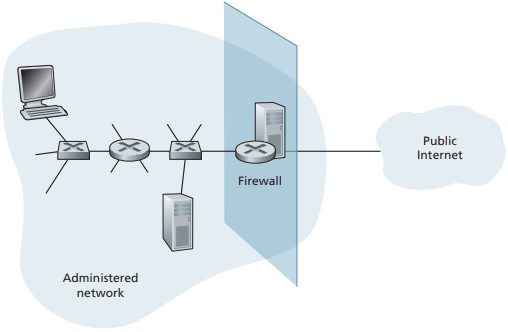
\includegraphics[width=0.95\linewidth]{cap22/packet_filter.png}
\end{minipage}\hfill
\begin{minipage}{0.51\linewidth}
\begin{itemize}
  \item \textbf{Tutto} il traffico in entrata e in uscita dovrebbe passare per il firewall, e solo il traffico \textbf{autorizzato} (secondo la politica di
        sicurezza locale) può passare.
  \item Il firewall fa da \textbf{unico punto di accesso} alla rete pubblica, ma le grandi organizzazioni possono avere più livelli di firewall o
        firewall distribuiti.
  \item Il firewall stesso deve essere \textbf{immune alle intrusioni}: se viene compromesso, dà un falso senso di sicurezza.
\end{itemize}
\end{minipage}
\caption{Un firewall tra la rete amministrata e la rete pubblica.}
\end{figure}

Vediamo tre approcci: il \textbf{filtraggio tradizionale} dei pacchetti, il \textbf{filtraggio stateful} e l'\textbf{application gateway}.

% ══════════════════════════════════════════════════════════════
\section{Il filtraggio tradizionale dei pacchetti}
% ══════════════════════════════════════════════════════════════

\begin{itemize}
    \item Un \textbf{filtro di pacchetti} è di solito realizzato sul \textbf{gateway}, il router che collega la rete locale all'ISP.
    \item Esamina \textbf{ogni singolo datagramma} e decide se accettarlo o scartarlo in base a regole specificate dall'amministratore. Si possono avere
          regole diverse per i datagrammi in entrata e in uscita, o per le singole interfacce.
\end{itemize}

Le regole si basano tipicamente su:

\begin{itemize}
    \item indirizzo IP sorgente o destinazione;
    \item tipo di protocollo nel campo del datagramma IP (TCP, UDP, ICMP, \dots);
    \item porta sorgente e destinazione;
    \item bit dei flag TCP (SYN, ACK, \dots);
    \item \dots
\end{itemize}

\begin{table}[H]
\centering
\begin{tabular}{p{6cm}p{8cm}}
\toprule
\textbf{Politica} & \textbf{Impostazione del firewall} \\
\midrule
Solo traffico Web in uscita & scartare tutti i segmenti TCP SYN in uscita con porta di destinazione diversa da 80 \\
Niente streaming (non critico) & scartare il traffico UDP in entrata non essenziale \\
Non rispondere ai ping dall'esterno & scartare le risposte ICMP ping in uscita (echo reply) \\
Telnet solo con host fidati & inoltrare i datagrammi Telnet (porta 23) solo da e verso un elenco di indirizzi \\
\bottomrule
\end{tabular}
\caption{Esempi di politiche e relative regole.}
\end{table}

\warning{I filtri non proteggono dallo spoofing}{
    Politiche basate su indirizzi e porte non proteggono dallo \textbf{spoofing}: un pacchetto con indirizzo sorgente falsificato su quello di un host
    fidato passa il filtro.
}

\subsection{Le access control list}

Nei router le regole del firewall sono realizzate con le \textbf{access control list} (ACL). Consideriamo l'ACL dell'interfaccia che collega il
router all'ISP, per un'organizzazione con indirizzi \texttt{222.22/16} che vuole lasciar passare \textbf{solo il traffico Web}:

\begin{table}[H]
\centering
\small
\begin{tabular}{lllllll}
\toprule
\textbf{Azione} & \textbf{IP sorgente} & \textbf{IP destinazione} & \textbf{Protocollo} & \textbf{Porta sorg.} & \textbf{Porta dest.} & \textbf{Flag} \\
\midrule
allow & 222.22/16 & esterno a 222.22/16 & TCP & $>$ 1023 & 80 & qualsiasi \\
allow & esterno a 222.22/16 & 222.22/16 & TCP & 80 & $>$ 1023 & ACK \\
allow & 222.22/16 & esterno a 222.22/16 & UDP & $>$ 1023 & 53 & --- \\
allow & esterno a 222.22/16 & 222.22/16 & UDP & 53 & $>$ 1023 & --- \\
deny & tutto & tutto & tutto & tutto & tutto & tutto \\
\bottomrule
\end{tabular}
\caption{Una ACL che permette solo il traffico Web (le regole si leggono dall'alto: vale la prima che corrisponde).}
\end{table}

\begin{enumerate}
    \item La prima regola lascia \textbf{uscire} qualsiasi pacchetto TCP con porta di destinazione 80.
    \item La seconda lascia \textbf{entrare} qualsiasi pacchetto TCP con porta sorgente 80 e flag \textbf{ACK = 1} (tutti i messaggi Web di risposta portano
          un ACK, mentre un tentativo di aprire una connessione dall'esterno avrebbe SYN senza ACK).
    \item La terza e la quarta insieme permettono ai pacchetti \textbf{DNS} di uscire ed entrare (senza DNS non si navigherebbe).
    \item L'ultima nega tutto il resto.
\end{enumerate}

\subsection{Il limite: il filtraggio è stateless}

\warning{Pacchetti ACK falsi}{
    Il filtraggio tradizionale è \textbf{senza stato}: esamina ogni pacchetto da solo. Per quanto restrittiva, la tabella precedente lascia entrare
    \textbf{qualsiasi} pacchetto dall'esterno con ACK = 1 e porta sorgente 80, anche se non fa parte di nessuna connessione aperta dall'interno.
    Pacchetti di questo tipo sono noti per essere usati negli attacchi DoS. La soluzione ingenua sarebbe bloccare anche i pacchetti TCP ACK, ma
    impedirebbe agli utenti interni di navigare sul Web.
}

% ══════════════════════════════════════════════════════════════
\section{Il filtraggio stateful}
% ══════════════════════════════════════════════════════════════

\dfn{Filtro stateful}{
    I \textbf{filtri stateful} risolvono il problema tenendo traccia di \textbf{tutte le connessioni TCP in corso} in una \textbf{tabella delle
    connessioni}, per capire se il traffico appartiene a una connessione legittima.
    \begin{itemize}
      \item Il firewall riconosce l'\textbf{inizio} di una nuova connessione (la sequenza SYN, SYNACK, ACK del three-way handshake) e la sua
            \textbf{fine} (il pacchetto FIN).
      \item Può anche assumere (in modo conservativo) che la connessione sia finita quando non vede attività per un certo tempo (per esempio 60 secondi).
    \end{itemize}
}

\begin{figure}[H]
    \centering
    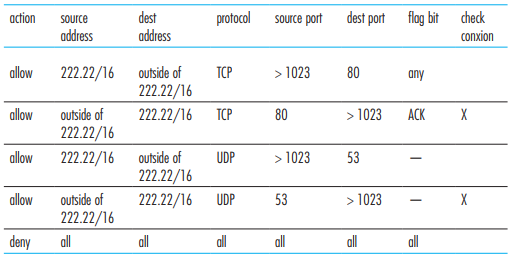
\includegraphics[width=0.65\linewidth]{cap22/stateful_table.png}
    \caption{L'ACL di un filtro stateful: la colonna ``check connection'' indica le regole che richiedono di verificare la tabella delle connessioni. In questo caso sono ammessi solo i pacchetti ACK che appartengono a connessioni già stabilite.}
\end{figure}

Una tabella stateful ha di solito una colonna ``\emph{check connection}'' che indica se un pacchetto deve far parte di una connessione già
stabilita: un pacchetto con ACK = 1 in arrivo dall'esterno passa solo se nella tabella c'è una connessione aperta dall'interno con gli stessi
indirizzi e porte.

% ══════════════════════════════════════════════════════════════
\section{L'application gateway}
% ══════════════════════════════════════════════════════════════

I filtri visti finora controllano soprattutto indirizzi IP e porte. Ma può servire permettere o negare funzionalità in base agli \textbf{utenti} o
all'\textbf{applicazione}, per esempio:

\begin{itemize}
    \item solo i tecnici possono usare certi protocolli (come Telnet verso l'esterno), negati agli utenti normali;
    \item all'interno di un protocollo sono permessi solo certi tipi di messaggi o comandi.
\end{itemize}

Compiti del genere vanno oltre le capacità dei filtri tradizionali e stateful: l'identità degli utenti interni è un dato applicativo, e non compare
negli header IP/TCP/UDP.

\dfn{Application gateway}{
    Un \textbf{application gateway} (o \emph{application-level gateway}, ALG) permette di filtrare i pacchetti in base ai \textbf{dati di livello
    applicativo}. È realizzato di solito come un \textbf{server separato} che lavora insieme al firewall.
}

\begin{figure}[H]
\centering
\begin{minipage}{0.4\linewidth}\centering
  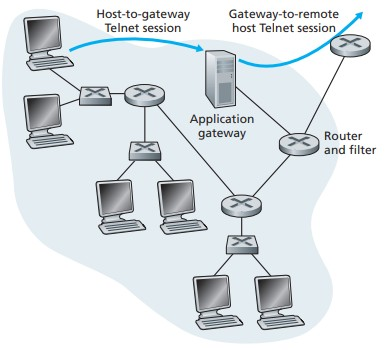
\includegraphics[width=0.95\linewidth]{cap22/app_gateway.png}
\end{minipage}\hfill
\begin{minipage}{0.56\linewidth}
\begin{itemize}
  \item L'idea è \textbf{negare tutte le connessioni} di un certo protocollo (per esempio Telnet) \textbf{tranne} quelle da e verso l'application gateway.
  \item Un utente che vuole usare il protocollo ristretto deve prima \textbf{autenticarsi presso il gateway} (nome utente e password).
  \item Il server controlla se l'utente ha il permesso per quel protocollo.
  \item Se sì, tutte le richieste e le risposte vengono inoltrate attraverso il gateway (che fa da \textbf{proxy}).
\end{itemize}
Le reti interne hanno spesso più application gateway, per protocolli diversi (Telnet, HTTP, FTP, posta).
\end{minipage}
\caption{Un gateway per Telnet: sessione host--gateway e sessione gateway--host remoto, con un router che filtra tutto il resto.}
\end{figure}

\warning{Gli svantaggi}{
    \begin{itemize}
      \item Serve un application gateway \textbf{diverso per ogni applicazione}.
      \item C'è una \textbf{penalità di prestazioni} dovuta al proxy (soprattutto con molti utenti).
      \item Il software sugli host deve sapere \textbf{come usare} l'application gateway.
    \end{itemize}
}

% ══════════════════════════════════════════════════════════════
\section{Gli Intrusion Detection System}
% ══════════════════════════════════════════════════════════════

Per rilevare certi tipi di attacco serve un'\textbf{ispezione profonda dei pacchetti} (\emph{deep packet inspection}): controllare, anche nel
contenuto, schemi di attacco noti o traffico sospetto.

\dfn{IDS e IPS}{
    Un \textbf{Intrusion Detection System} (IDS) è un insieme di dispositivi specializzati che \textbf{monitorano la rete} cercando pacchetti sospetti.
    \begin{itemize}
      \item Il suo compito principale è \textbf{riconoscere} i pacchetti potenzialmente malevoli e \textbf{allertare} l'amministratore di rete (che poi
            deciderà cosa fare).
      \item Se può anche \textbf{bloccare} (filtrare) i pacchetti sospetti, si parla di \textbf{Intrusion Prevention System} (IPS).
    \end{itemize}
}

Le organizzazioni usano gli IDS per rilevare un'ampia gamma di attacchi (o di potenziali attacchi):

\begin{itemize}
    \item scansioni della rete o delle porte (per esempio con nmap);
    \item flooding DoS;
    \item worm e virus;
    \item \dots
\end{itemize}

\begin{figure}[H]
    \centering
    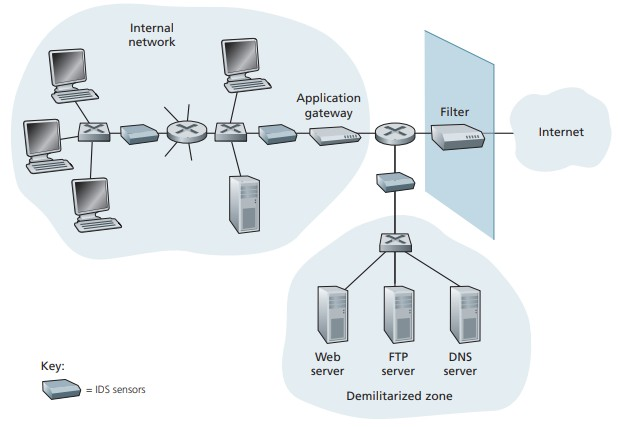
\includegraphics[width=0.65\linewidth]{cap22/ids.png}
    \caption{Una rete con filtro, application gateway, sensori IDS e zona demilitarizzata (da Kurose).}
\end{figure}

Il sistema è spesso composto da:

\begin{itemize}
    \item uno o più \textbf{sensori IDS};
    \item un unico \textbf{processore IDS centrale}, che raccoglie e integra le informazioni e invia gli allarmi.
\end{itemize}

Gli IDS possono essere:

\begin{itemize}
    \item \textbf{basati su firme} (\emph{signature-based}): mantengono un ampio database di \textbf{firme di attacco}, cioè insiemi di regole legate a
          un'attività di intrusione (è il tipo più comune). Non riconoscono attacchi nuovi;
    \item \textbf{basati su anomalie} (\emph{anomaly-based}): costruiscono un \textbf{profilo del traffico} normale e segnalano i flussi statisticamente
          insoliti. Possono scoprire attacchi nuovi, ma è difficile distinguere il traffico anomalo da quello semplicemente raro.
\end{itemize}

% ══════════════════════════════════════════════════════════════
\section{La zona demilitarizzata (DMZ)}
% ══════════════════════════════════════════════════════════════

Nelle reti grandi capita spesso di dover avere \textbf{due livelli di sicurezza} per dispositivi diversi: i server che devono comunicare con il mondo
esterno, per esempio, hanno bisogno di un filtraggio più blando.

\dfn{Zona demilitarizzata (DMZ)}{
    Una \textbf{zona demilitarizzata} (DMZ) è una regione a \textbf{bassa sicurezza}, con restrizioni limitate, in cui ospitare i server che devono
    essere raggiungibili dall'esterno (Web, FTP, DNS). Un approccio tipico è mettere la DMZ \textbf{tra due firewall}: uno esterno, meno restrittivo, e
    uno interno, più restrittivo.
}

\begin{figure}[H]
\centering
\begin{tikzpicture}[every node/.style={font=\footnotesize\sffamily}]
  \node[netcloud, minimum width=2.4cm] (i) at (0,0) {Internet};
  \node[draw, fill=netred!30, minimum width=0.5cm, minimum height=1.8cm] (f1) at (2.6,0) {};
  \node[below=2pt of f1, align=center] {firewall\\esterno};
  \node[draw=netorange, thick, dashed, rounded corners, fill=netorange!8, minimum width=3.4cm, minimum height=2.4cm] (dmz) at (5.6,0) {};
  \node[anchor=north, text=netorange, font=\footnotesize\bfseries\sffamily] at (dmz.north) {DMZ};
  \node at (4.8,-0.3) {\icon[0.45cm]{server}}; \node at (5.6,-0.3) {\icon[0.45cm]{server}}; \node at (6.4,-0.3) {\icon[0.45cm]{server}};
  \node[font=\scriptsize\sffamily] at (5.6,-0.95) {Web \quad FTP \quad DNS};
  \node[draw, fill=netred!60, minimum width=0.5cm, minimum height=1.8cm] (f2) at (8.6,0) {};
  \node[below=2pt of f2, align=center] {firewall interno\\+ app. gateway};
  \node[draw=netgreen!60!black, thick, rounded corners, fill=netgreen!8, minimum width=3.2cm, minimum height=2.4cm] (lan) at (11.6,0) {};
  \node[anchor=north, text=netgreen!50!black, font=\footnotesize\bfseries\sffamily] at (lan.north) {rete interna};
  \node at (11,-0.3) {\icon[0.6cm]{pc}}; \node at (12.1,-0.3) {\icon[0.7cm]{laptop}};
  \draw[wired] (i) -- (f1); \draw[wired] (f1) -- (dmz); \draw[wired] (dmz) -- (f2); \draw[wired] (f2) -- (lan);
  \node[text width=4cm, align=center, text=netred] at (5.6,-1.8) {filtraggio blando, sensori IDS};
  \node[text width=4cm, align=center, text=netgreen!50!black] at (11.6,-1.8) {alta sicurezza, sensori IDS};
\end{tikzpicture}
\caption{La DMZ tra due firewall.}
\end{figure}

\begin{itemize}
    \item La regione ad \textbf{alta sicurezza} è protetta da un filtro di pacchetti e da un application gateway, ed è monitorata da sensori IDS.
    \item La regione a \textbf{bassa sicurezza} (la DMZ) è protetta solo dal filtro ed è monitorata dai sensori.
\end{itemize}

\info{Oltre la sicurezza: la privatezza}{
    Crittografia e firewall proteggono i contenuti, ma chi osserva la rete vede comunque \textbf{chi} parla con \textbf{chi} (gli indirizzi IP non sono
    cifrati). Per nascondere anche questo esistono reti di anonimizzazione come \textbf{Tor}, che fa passare il traffico cifrato attraverso più nodi, e
    sistemi come \textbf{Whonix} che instradano tutto il traffico di una macchina virtuale attraverso Tor.
}

% ══════════════════════════════════════════════════════════════
\section{Riepilogo}
% ══════════════════════════════════════════════════════════════

\riepilogo{
\begin{itemize}
    \item \textbf{Autenticazione}: l'IP si falsifica, la password si intercetta, la password cifrata si ripete (\textbf{playback}); la soluzione è il
          \textbf{nonce}, usato una sola volta.
    \item \textbf{SSL/TLS} protegge TCP: \textbf{handshake} (certificato del server, master secret cifrato con la chiave pubblica), \textbf{derivazione}
          di 4 chiavi (cifratura e MAC per ogni direzione), \textbf{trasferimento} a record con MAC e numero di sequenza. HTTPS = HTTP + TLS.
    \item \textbf{Firewall}: filtraggio \textbf{tradizionale} (ACL su indirizzi, porte, flag; stateless), \textbf{stateful} (tabella delle connessioni),
          \textbf{application gateway} (dati applicativi, utenti, proxy).
    \item \textbf{IDS/IPS}: ispezione profonda, basati su firme o su anomalie; la \textbf{DMZ} ospita i server pubblici tra due firewall.
\end{itemize}
}
     % Autenticazione, TLS, firewall

  % ------------------------------------------------------------------
  \part{Esercizi}
  % ------------------------------------------------------------------
  \chapter{Esercizi sui fondamenti}

Questa parte raccoglie gli esercizi svolti, organizzati per livello. Molti riprendono gli esempi visti nei capitoli teorici
\textbf{con numeri diversi}, così da potersi esercitare davvero; altri sono le esercitazioni di laboratorio proposte a lezione,
con lo svolgimento completo. Il consiglio è sempre lo stesso: \textbf{provare prima da soli}, e solo dopo leggere la soluzione.

% ══════════════════════════════════════════════════════════════
\section{Ritardi e tempi di trasmissione}
% ══════════════════════════════════════════════════════════════

\info{Richiamo: i ritardi di un pacchetto}{
    Un pacchetto che attraversa un nodo accumula quattro ritardi:
    $$d_{\text{nodo}} = d_{\text{elab}} + d_{\text{coda}} + d_{\text{trasm}} + d_{\text{prop}}$$
    \begin{itemize}
      \item $d_{\text{elab}}$: elaborazione (controllo degli errori, scelta dell'uscita), tipicamente microsecondi;
      \item $d_{\text{coda}}$: attesa in coda, dipende dal traffico;
      \item $d_{\text{trasm}} = L/R$: tempo per ``spingere'' sul collegamento tutti gli $L$ bit al rate $R$. Dipende dalla
            \textbf{dimensione del pacchetto} e dal \textbf{rate}, \emph{non} dalla distanza;
      \item $d_{\text{prop}} = d/s$: tempo che il segnale impiega a percorrere la distanza $d$ alla velocità $s$
            ($2$--$3 \cdot 10^8$ m/s). Dipende dalla \textbf{distanza}, \emph{non} dal pacchetto.
    \end{itemize}
}

\begin{esercizio}{Trasmissione contro propagazione}
Un pacchetto di $L = 1000$ byte viaggia su un collegamento lungo $d = 2500$ km, con rate $R = 10$ Mb/s e velocità di
propagazione $s = 2{,}5 \cdot 10^8$ m/s.
\begin{enumerate}[label=(\alph*)]
    \item Calcolare il tempo di trasmissione e il tempo di propagazione. Quale dei due domina?
    \item Ripetere il calcolo con $R = 1$ Gb/s. Che cosa cambia?
    \item Quanto è ``lungo'', in metri, un singolo bit sul cavo nei due casi?
    \item Un collegamento via satellite geostazionario (quota $36\,000$ km, $s = 3\cdot 10^8$ m/s) collega due stazioni a
          terra. Quanto vale il ritardo di propagazione tra le due stazioni?
\end{enumerate}
\end{esercizio}

\svolgimento
\textbf{(a)} Il pacchetto è di $1000 \cdot 8 = 8000$ bit.
$$d_{\text{trasm}} = \frac{L}{R} = \frac{8000}{10^7} = 0{,}8 \text{ ms} \qquad
  d_{\text{prop}} = \frac{d}{s} = \frac{2{,}5 \cdot 10^6 \text{ m}}{2{,}5 \cdot 10^8 \text{ m/s}} = 10 \text{ ms}$$
Domina la propagazione (12,5 volte più grande); il totale, senza code ed elaborazione, è $10{,}8$ ms.

\textbf{(b)} Con $R = 10^9$ b/s: $d_{\text{trasm}} = 8000/10^9 = 8\ \mu$s, mentre $d_{\text{prop}}$ resta $10$ ms. Il totale scende
solo a $10{,}008$ ms: aumentare la banda \textbf{non accorcia la propagazione}.

\textbf{(c)} In un secondo escono $R$ bit che si distribuiscono su $s$ metri, quindi ogni bit occupa $s/R$ metri:
\begin{itemize}
    \item a 10 Mb/s: $2{,}5\cdot 10^8 / 10^7 = 25$ m per bit (il pacchetto intero è lungo $200$ km);
    \item a 1 Gb/s: $2{,}5\cdot 10^8 / 10^9 = 25$ cm per bit.
\end{itemize}

\textbf{(d)} Il segnale sale e scende: $d = 2 \cdot 36\,000$ km $= 7{,}2\cdot 10^7$ m, quindi
$d_{\text{prop}} = 7{,}2\cdot 10^7 / 3\cdot 10^8 = 0{,}24$ s. Un RTT via satellite supera così il mezzo secondo, ed è per questo
che le telefonate satellitari hanno quel fastidioso ritardo.

\warning{L'analogia dell'autostrada}{
    Pensate a una colonna di 10 auto (i bit) che attraversa un casello (il router) e poi percorre 100 km di autostrada. Il
    tempo per far passare \emph{tutte} le auto dal casello è il ritardo di \textbf{trasmissione}; il tempo che ciascuna
    impiega a percorrere l'autostrada è il ritardo di \textbf{propagazione}. Aprire più caselli (più banda) non rende
    l'autostrada più corta.
}

\begin{esercizio}{Messaggio intero o pacchetti?}
Un messaggio di $8 \cdot 10^6$ bit va dalla sorgente alla destinazione attraverso due router, cioè su $N = 3$ collegamenti
da $R = 2$ Mb/s. Si trascurino propagazione, code ed elaborazione.
\begin{enumerate}[label=(\alph*)]
    \item Quanto tempo serve se il messaggio viene inviato \textbf{intero} (commutazione di messaggio, store-and-forward)?
    \item Quanto tempo serve se viene diviso in $P = 800$ pacchetti da $10\,000$ bit ciascuno? Quando arriva il primo pacchetto?
    \item Ricavare la formula generale e spiegare da dove viene il guadagno.
\end{enumerate}
\end{esercizio}

\svolgimento
\textbf{(a)} Ogni nodo deve ricevere tutto il messaggio prima di inoltrarlo. Ogni collegamento richiede
$8\cdot 10^6 / 2\cdot 10^6 = 4$ s, quindi il totale è $3 \cdot 4 = 12$ s.

\textbf{(b)} Ogni pacchetto richiede $L/R = 10^4 / 2\cdot 10^6 = 5$ ms per collegamento.
\begin{itemize}
    \item Il \textbf{primo} pacchetto arriva dopo $3 \cdot 5 = 15$ ms.
    \item La sorgente finisce di trasmettere l'\textbf{ultimo} pacchetto dopo $800 \cdot 5$ ms $= 4$ s; da lì servono altri 2
          collegamenti, cioè $10$ ms. Il messaggio è completo dopo $4{,}01$ s.
\end{itemize}

\textbf{(c)} La figura mostra il caso di $P = 3$ pacchetti su $N = 3$ collegamenti, con il tempo diviso in intervalli da $L/R$.

\begin{figure}[H]
\centering
\begin{tikzpicture}[x=1.25cm, y=0.8cm, every node/.style={font=\scriptsize\sffamily}]
  \foreach \r/\n in {0/{collegamento 1}, 1/{collegamento 2}, 2/{collegamento 3}} \node[anchor=east] at (0,-\r-0.5) {\n};
  \foreach \t in {0,...,5} \draw[black!25] (\t,0) -- (\t,-3);
  \foreach \t in {1,...,5} \node at (\t-0.5,0.3) {$t_{\t}$};
  \foreach \r in {0,...,3} \draw[black!25] (0,-\r) -- (5,-\r);
  \foreach \r in {0,1,2} {
    \foreach \p/\c in {1/netblue!55, 2/netgreen!55, 3/netorange!60} {
      \pgfmathtruncatemacro{\s}{\r+\p-1}
      \fill[\c] (\s+0.05,-\r-0.1) rectangle (\s+0.95,-\r-0.9);
      \node at (\s+0.5,-\r-0.5) {p\p};
    }
  }
  \draw[decorate, decoration={brace, amplitude=5pt, mirror}] (0,-3.15) -- (5,-3.15) node[midway, below=6pt] {$(P + N - 1)\cdot L/R = (3+3-1)\cdot L/R = 5\cdot L/R$};
\end{tikzpicture}
\caption{Con i pacchetti i collegamenti lavorano \emph{in parallelo}, come una catena di montaggio.}
\end{figure}

Il primo pacchetto impiega $N$ intervalli, e ciascuno dei $P-1$ successivi arriva un intervallo dopo il precedente:
$$T = (P + N - 1)\cdot\frac{L}{R} = (800 + 3 - 1) \cdot 5 \text{ ms} = 4{,}01 \text{ s}$$
Con il messaggio intero, invece, $T = N \cdot P \cdot L/R$: i collegamenti lavorano \emph{uno alla volta}. Dividere in pacchetti
permette ai router di lavorare contemporaneamente; inoltre un errore costringe a ritrasmettere solo un pacchetto, e più
comunicazioni possono alternarsi sullo stesso collegamento. Il prezzo sono gli header di ogni pacchetto e la necessità di
riordinarli a destinazione.

\begin{esercizio}{Throughput e collo di bottiglia}
Un server invia un file di 4 MB a un client attraverso tre collegamenti in serie: $R_1 = 500$ kb/s, $R_2 = 2$ Mb/s,
$R_3 = 1$ Mb/s.
\begin{enumerate}[label=(\alph*)]
    \item Qual è il throughput del trasferimento, in assenza di altro traffico?
    \item Quanto dura, approssimativamente, il trasferimento?
    \item Il collegamento centrale viene condiviso in parti uguali da 10 trasferimenti contemporanei. Come cambiano le risposte?
\end{enumerate}
\end{esercizio}

\svolgimento
\begin{center}
\begin{tikzpicture}[every node/.style={font=\scriptsize\sffamily}]
  \node (s) at (0,0) {\icon[0.7cm]{server}}; \node[below=-1pt of s] {server};
  \node (r1) at (3,0) {\icon[0.8cm]{router}};
  \node (r2) at (6,0) {\icon[0.8cm]{router}};
  \node (c) at (9,0) {\icon[0.8cm]{laptop}}; \node[below=-1pt of c] {client};
  \draw[wired, line width=1pt] (s) -- node[above] {$R_1 = 500$ kb/s} (r1);
  \draw[wired, line width=3pt] (r1) -- node[above] {$R_2 = 2$ Mb/s} (r2);
  \draw[wired, line width=2pt] (r2) -- node[above] {$R_3 = 1$ Mb/s} (c);
  \node[text=netred] at (1.5,-0.45) {collo di bottiglia};
\end{tikzpicture}
\end{center}

\textbf{(a)} Il throughput è limitato dal collegamento più lento: $\min\{R_1, R_2, R_3\} = 500$ kb/s.

\textbf{(b)} $4$ MB $= 32 \cdot 10^6$ bit, quindi $T = 32\cdot 10^6 / 5 \cdot 10^5 = 64$ s.

\textbf{(c)} Ogni trasferimento ottiene $R_2/10 = 200$ kb/s sul collegamento centrale, che diventa il nuovo collo di bottiglia:
throughput $= \min\{500, 200, 1000\} = 200$ kb/s, e il trasferimento dura $32\cdot 10^6 / 2\cdot 10^5 = 160$ s. Il collo di
bottiglia non è sempre il collegamento con il rate più basso: dipende anche da \textbf{quanto è condiviso}.

% ══════════════════════════════════════════════════════════════
\section{Commutazione di circuito e di pacchetto}
% ══════════════════════════════════════════════════════════════

\begin{esercizio}{Quanti utenti su un collegamento}
Un collegamento da 1 Mb/s è condiviso da utenti che, quando sono attivi, trasmettono a 100 kb/s; ogni utente è attivo in
media il 10\% del tempo, in modo indipendente dagli altri.
\begin{enumerate}[label=(\alph*)]
    \item Con la commutazione di circuito, quanti utenti si possono servire?
    \item Con la commutazione di pacchetto e 35 utenti, qual è la probabilità che esattamente $n$ utenti siano attivi?
    \item Qual è la probabilità che più di 10 utenti siano attivi contemporaneamente? Commentare.
\end{enumerate}
\end{esercizio}

\svolgimento
\textbf{(a)} Ogni circuito riserva 100 kb/s anche quando l'utente tace: $1000/100 = 10$ utenti.

\textbf{(b)} Ogni utente è attivo con probabilità $p = 0{,}1$, indipendentemente dagli altri: il numero di utenti attivi segue
una \textbf{distribuzione binomiale}
$$P(n \text{ attivi}) = \binom{35}{n}\, p^n (1-p)^{35-n}$$
Per esempio $P(0) \approx 0{,}025$, $P(3) \approx 0{,}225$ (il valore più probabile), $P(10) \approx 0{,}0013$.

\textbf{(c)} Il collegamento va in sovraccarico solo se ci sono almeno 11 utenti attivi:
$$P(n > 10) = 1 - \sum_{n=0}^{10} \binom{35}{n}\, 0{,}1^n\, 0{,}9^{35-n} \approx 1 - 0{,}99958 = 0{,}00042$$
Circa \textbf{4 volte su diecimila}. La commutazione di pacchetto serve quindi 3,5 volte gli utenti del circuito, con prestazioni
quasi identiche: è il guadagno della \textbf{multiplazione statistica}, che sfrutta il fatto che il traffico dati è
\emph{a raffiche} (\emph{bursty}). Il prezzo è che, in quei rari momenti, i pacchetti si accodano e possono andare persi: non c'è
più una garanzia.

\begin{esercizio}{Un file su un circuito TDM}
Quanto tempo serve per inviare un file di $640\,000$ bit dall'host A all'host B su una rete a commutazione di circuito, se tutti
i collegamenti sono da $1{,}536$ Mb/s, ognuno usa TDM con 24 slot, e servono 500 ms per stabilire il circuito? Quanto
servirebbe se il collegamento fosse tutto per noi?
\end{esercizio}

\svolgimento
Con TDM a 24 slot, a ogni circuito spetta $1{,}536 / 24 = 64$ kb/s. Il trasferimento dura
$640\,000 / 64\,000 = 10$ s, a cui si sommano i $0{,}5$ s di instaurazione: $\mathbf{10{,}5}$ \textbf{s}.

Se potessimo usare l'intero collegamento, la trasmissione durerebbe $640\,000 / 1\,536\,000 \approx 0{,}42$ s (per
collegamento). Il circuito ci \textbf{garantisce} i 64 kb/s, ma ci impedisce di usare la capacità lasciata libera dagli altri.

% ══════════════════════════════════════════════════════════════
\section{Topologie}
% ══════════════════════════════════════════════════════════════

\begin{esercizio}{Contare collegamenti e porte}
Una rete ha $n = 8$ nodi.
\begin{enumerate}[label=(\alph*)]
    \item Quanti collegamenti servono con topologia a maglia completa, a stella, ad anello e a bus? Quante porte deve avere ogni
          nodo nella maglia completa?
    \item Si aggiunge un nono nodo: quanti collegamenti in più servono in ciascun caso?
    \item Che cosa succede, in ciascuna topologia, se si guasta un singolo collegamento? E se si guasta il nodo centrale della stella?
\end{enumerate}
\end{esercizio}

\svolgimento
\textbf{(a)} e \textbf{(b)}:
\begin{table}[H]
\centering
\begin{tabular}{lccc}
\toprule
\textbf{Topologia} & \textbf{Collegamenti con 8 nodi} & \textbf{Con 9 nodi} & \textbf{In più} \\
\midrule
Maglia completa & $\frac{8\cdot 7}{2} = 28$ & $\frac{9 \cdot 8}{2} = 36$ & 8 \\
Stella & 8 (più il nodo centrale) & 9 & 1 \\
Anello & 8 & 9 & 1 (se ne toglie uno e se ne aggiungono due) \\
Bus & 1 dorsale + 8 derivazioni & 1 + 9 & 1 derivazione \\
\bottomrule
\end{tabular}
\caption{Collegamenti richiesti dalle diverse topologie.}
\end{table}
Nella maglia completa ogni nodo è collegato a tutti gli altri: servono $n - 1 = 7$ porte per nodo. Aggiungere un nodo costa
$n$ collegamenti nuovi e una porta in più su \emph{ogni} nodo esistente: è la crescita quadratica che rende la maglia completa
impraticabile per reti grandi.

\textbf{(c)} Guasto di un collegamento:
\begin{itemize}
    \item \textbf{maglia completa}: nessun effetto sulla connettività, esistono altri cammini;
    \item \textbf{stella}: resta isolato solo il nodo di quel collegamento;
    \item \textbf{anello}: se l'anello è unidirezionale la rete si interrompe; se è bidirezionale (o doppio) i messaggi
          possono girare nell'altro verso;
    \item \textbf{bus}: se si guasta la dorsale la rete si divide in due parti (e il segnale riflesso può disturbare tutti).
\end{itemize}
Se si guasta il \textbf{centro della stella} si ferma tutta la rete: è il suo \emph{single point of failure}.

\begin{esercizio}{Perché esistono gli IXP}
Sei ISP regionali vogliono scambiarsi traffico direttamente, a coppie. Quanti collegamenti di peering servono? E se si
incontrano tutti in un IXP? Ripetere con 50 ISP.
\end{esercizio}

\svolgimento
Collegare tutti con tutti è una maglia completa: $\frac{6 \cdot 5}{2} = 15$ collegamenti. Con un IXP ogni ISP porta un solo
collegamento al punto di scambio: $6$ collegamenti. Con 50 ISP: $\frac{50 \cdot 49}{2} = 1225$ contro $50$. L'IXP trasforma una
maglia in una \textbf{stella}, ed è il motivo per cui questi punti neutrali di scambio si sono diffusi.

% ══════════════════════════════════════════════════════════════
\section{Stratificazione e incapsulamento}
% ══════════════════════════════════════════════════════════════

\begin{esercizio}{Quanto pesano gli header}
Un'applicazione invia messaggi di $M$ byte. Lungo la pila TCP/IP su Ethernet si aggiungono un header TCP da 20 byte, un header
IP da 20 byte e 18 byte di header e trailer Ethernet.
\begin{enumerate}[label=(\alph*)]
    \item Che frazione dei byte trasmessi è occupata dagli header se $M = 100$ byte? E se $M = 1460$ byte?
    \item In una sessione remota ogni tasto premuto invia 1 byte. Che frazione è overhead?
    \item Ricavare la formula per una pila di $n$ strati, ognuno dei quali aggiunge $h$ byte.
\end{enumerate}
\end{esercizio}

\svolgimento
Gli header valgono in tutto $h_{\text{tot}} = 20 + 20 + 18 = 58$ byte.

\begin{center}
\begin{tikzpicture}[every node/.style={font=\scriptsize\sffamily}]
  \node[field, fill=llink, minimum width=1.3cm] (e) at (0,0) {Ethernet 14};
  \node[field, fill=lnet, minimum width=1.2cm, right=0pt of e] (i) {IP 20};
  \node[field, fill=ltra, minimum width=1.2cm, right=0pt of i] (t) {TCP 20};
  \node[field, fill=lapp, minimum width=4.2cm, right=0pt of t] (m) {messaggio: $M$ byte};
  \node[field, fill=llink, minimum width=1.2cm, right=0pt of m] {CRC 4};
\end{tikzpicture}
\end{center}

\textbf{(a)}
$$M = 100: \quad \frac{58}{100 + 58} \approx 36{,}7\% \qquad\qquad M = 1460: \quad \frac{58}{1460 + 58} \approx 3{,}8\%$$

\textbf{(b)} $\dfrac{58}{1 + 58} \approx 98{,}3\%$: per spedire un byte se ne trasmettono 59. I messaggi piccoli sono i più
penalizzati dalla stratificazione.

\textbf{(c)} La frazione occupata dagli header è
$$\frac{n\,h}{M + n\,h}$$
che tende a 0 per messaggi grandi e a 1 per messaggi piccoli.

\begin{esercizio}{A quale livello?}
Per ciascuna voce indicare il livello della pila a cinque strati coinvolto e, dove ha senso, l'unità di dati.
\begin{enumerate}
    \item Scegliere il cammino di un pacchetto tra i router.
    \item Consegnare i dati al processo giusto, individuato da un numero di porta.
    \item Delimitare i frame e rilevare gli errori su un singolo collegamento.
    \item Trasformare i bit in segnali elettrici o luminosi.
    \item Chiedere una pagina Web a un server.
    \item Ritrasmettere dati persi lungo il percorso tra i due estremi.
    \item Tradurre un nome come \texttt{www.unina.it} in un indirizzo IP.
    \item Uno switch; un router; un hub (ripetitore).
\end{enumerate}
\end{esercizio}

\svolgimento
\begin{table}[H]
\centering
\begin{tabular}{clp{6.6cm}}
\toprule
\textbf{\#} & \textbf{Livello} & \textbf{Nota} \\
\midrule
1 & Rete & routing; unità: datagramma \\
2 & Trasporto & consegna processo-a-processo; unità: segmento \\
3 & Collegamento & consegna \emph{hop-to-hop}; unità: frame \\
4 & Fisico & unità: bit \\
5 & Applicazione & HTTP; unità: messaggio \\
6 & Trasporto & il trasferimento affidabile è di TCP (end-to-end) \\
7 & Applicazione & il DNS è un'applicazione che offre un servizio alle altre applicazioni \\
8 & Collegamento; Rete; Fisico & lo switch implementa 2 livelli, il router 3, l'hub solo il fisico \\
\bottomrule
\end{tabular}
\caption{Livelli e unità di dati.}
\end{table}

\begin{esercizio}{Che servizio serve?}
Per ciascuna applicazione scegliere il tipo di servizio più adatto tra i sei visti nel capitolo sulla stratificazione, e dire
se ci si aspetta che usi TCP o UDP.
(a) scaricare un file ISO; (b) una telefonata VoIP; (c) una query DNS; (d) stampare un libro diviso in pagine;
(e) pubblicità inviata in massa; (f) un messaggio con conferma di lettura.
\end{esercizio}

\svolgimento
\begin{itemize}
    \item \textbf{(a)} Flusso di byte affidabile (TCP): non può mancare nemmeno un byte.
    \item \textbf{(b)} Connessione inaffidabile (tipicamente UDP): un pacchetto perso è un piccolo ``click'', uno in ritardo è inutile.
    \item \textbf{(c)} Richiesta-risposta (UDP): una domanda, una risposta; se si perde, si ripete.
    \item \textbf{(d)} Flusso di messaggi affidabile: i confini tra le pagine vanno preservati.
    \item \textbf{(e)} Datagram inaffidabile: nessuno si preoccupa se qualche messaggio va perso.
    \item \textbf{(f)} Datagram con conferma: niente connessione, ma il mittente vuole sapere che il messaggio è arrivato.
\end{itemize}

\begin{esercizio}{Chi legge quale header}
L'host A invia una richiesta HTTP al server B. Il percorso attraversa uno switch, poi un router, poi arriva a B. Per ciascun
dispositivo dire fino a quale livello ``apre'' il pacchetto e quali campi legge o modifica.
\end{esercizio}

\svolgimento
\begin{figure}[H]
\centering
\begin{tikzpicture}[every node/.style={font=\scriptsize\sffamily}, lay/.style={minimum width=1.6cm, minimum height=0.45cm, font=\tiny\sffamily}]
  % host A
  \node[lay app, lay] (a5) at (0,0) {Applicazione};
  \node[lay tra, lay, below=0pt of a5] (a4) {Trasporto};
  \node[lay net, lay, below=0pt of a4] (a3) {Rete};
  \node[lay link, lay, below=0pt of a3] (a2) {Collegamento};
  \node[lay phy, lay, below=0pt of a2] (a1) {Fisico};
  \node[lay link, lay] (s2) at (3.3,-1.35) {Collegamento};
  \node[lay phy, lay, below=0pt of s2] (s1) {Fisico};
  \node[lay net, lay] (r3) at (6.6,-0.9) {Rete};
  \node[lay link, lay, below=0pt of r3] (r2) {Collegamento};
  \node[lay phy, lay, below=0pt of r2] (r1) {Fisico};
  \node[lay app, lay] (b5) at (9.9,0) {Applicazione};
  \node[lay tra, lay, below=0pt of b5] (b4) {Trasporto};
  \node[lay net, lay, below=0pt of b4] (b3) {Rete};
  \node[lay link, lay, below=0pt of b3] (b2) {Collegamento};
  \node[lay phy, lay, below=0pt of b2] (b1) {Fisico};
  \foreach \x/\n in {0/host A, 3.3/switch, 6.6/router, 9.9/server B} \node[font=\footnotesize\bfseries\sffamily] at (\x,0.55) {\n};
  \draw[very thick, netred, -{Stealth}, rounded corners=2pt] (0.95,0) -- (0.95,-2.25) -- (2.35,-2.25) -- (2.35,-1.0) -- (4.25,-1.0)
     -- (4.25,-2.25) -- (5.65,-2.25) -- (5.65,-0.55) -- (7.55,-0.55) -- (7.55,-2.25) -- (8.85,-2.25) -- (8.85,0);
\end{tikzpicture}
\caption{Il pacchetto sale lungo la pila solo fino al livello che il dispositivo implementa.}
\end{figure}

\begin{itemize}
    \item \textbf{Switch} (livello 2): legge l'header Ethernet, in particolare il \textbf{MAC di destinazione}, per scegliere la
          porta d'uscita. Non modifica il frame e non guarda dentro il payload.
    \item \textbf{Router} (livello 3): rimuove l'header Ethernet, legge l'\textbf{IP di destinazione} per scegliere l'uscita,
          \textbf{decrementa il TTL} e ricalcola il checksum IP, poi incapsula il datagramma in un \textbf{nuovo frame} con nuovi MAC.
          Non legge l'header TCP né la richiesta HTTP.
    \item \textbf{Server B}: decapsula tutti gli strati fino alla richiesta HTTP, che consegna al processo server individuato
          dalla porta di destinazione (80).
\end{itemize}
Ogni strato tratta il proprio payload come \textbf{opaco}: il router trasporta la richiesta HTTP senza sapere che esiste.

\begin{esercizio}{Simplex, half-duplex o full-duplex?}
Classificare: (a) una trasmissione televisiva; (b) una coppia di walkie-talkie; (c) una telefonata; (d) una tastiera
collegata a un computer; (e) un segmento Ethernet condiviso su hub; (f) un collegamento Ethernet commutato moderno.
\end{esercizio}

\svolgimento
(a) simplex; (b) half-duplex (si parla a turno, ``passo''); (c) full-duplex; (d) simplex; (e) half-duplex (una stazione
alla volta, altrimenti collisione); (f) full-duplex (coppie di fili separate per i due versi, niente collisioni).

\gbox{\iinfo\ Formule da ricordare}{primary!80!black}{
\begin{itemize}
    \item $d_{\text{trasm}} = L/R$; \quad $d_{\text{prop}} = d/s$; \quad lunghezza di un bit sul mezzo $= s/R$.
    \item $P$ pacchetti su $N$ collegamenti store-and-forward: $T = (P + N - 1)\cdot L/R$.
    \item Throughput end-to-end $= \min_i R_i$ (tenendo conto della condivisione).
    \item Maglia completa: $n(n-1)/2$ collegamenti; stella e anello: $n$.
    \item Overhead degli header: $n\,h / (M + n\,h)$.
\end{itemize}
}
      % Fondamenti
  \chapter{Esercizi sul livello applicativo}

% ══════════════════════════════════════════════════════════════
\section{Preparare Wireshark}
% ══════════════════════════════════════════════════════════════

Prima di svolgere gli esercizi di laboratorio serve un Wireshark funzionante e utilizzabile \textbf{da utente non-root}
(catturare pacchetti come root è sconsigliato: Wireshark analizza dati che arrivano dalla rete, cioè potenzialmente ostili).

\begin{lstlisting}[language=bash]
sudo apt update
sudo apt install wireshark          # rispondere "Sì" alla cattura per utenti non-root

getent group wireshark              # esiste il gruppo wireshark?
groups                              # l'utente ne fa parte?

sudo dpkg-reconfigure wireshark-common      # se serve cambiare la scelta fatta all'installazione
sudo usermod -aG wireshark $USER            # aggiungere l'utente al gruppo
newgrp wireshark                            # (oppure logout e login)

getcap /usr/bin/dumpcap             # deve mostrare cap_net_raw,cap_net_admin=eip
sudo setcap cap_net_raw,cap_net_admin+eip /usr/bin/dumpcap   # solo se mancano i permessi
\end{lstlisting}

\info{Chi cattura davvero i pacchetti}{
    La cattura non la fa l'interfaccia grafica ma il piccolo programma \texttt{dumpcap}, che ha bisogno delle
    \emph{capabilities} \texttt{cap\_net\_raw} (leggere pacchetti grezzi) e \texttt{cap\_net\_admin} (mettere l'interfaccia in
    modalità promiscua). Assegnarle solo a lui è più sicuro che eseguire Wireshark come root.
}

% ══════════════════════════════════════════════════════════════
\section{HTTP con Wireshark}
% ══════════════════════════════════════════════════════════════

\begin{esercizio}{Interazione base: GET e risposta}
\begin{enumerate}
    \item Avviare il browser e Wireshark, senza iniziare la cattura. Nel campo del filtro di visualizzazione scrivere \texttt{http}.
    \item Attendere poco più di un minuto (il motivo sarà chiaro alla fine), poi avviare la cattura.
    \item Visitare \url{http://www.columbia.edu/~fdc/sample.html} e fermare la cattura.
\end{enumerate}
Si vedranno la richiesta GET e la risposta del server. Espandere solo la sezione HTTP (Frame, Ethernet, IP e TCP chiuse) e
rispondere:
\begin{enumerate}[label=(\alph*)]
    \item Quale versione di HTTP usa il browser? E il server?
    \item Quali lingue il browser dichiara di accettare?
    \item Qual è l'indirizzo IP del proprio computer? E quello del server?
    \item Qual è il codice di stato restituito?
    \item Quando è stata modificata l'ultima volta la pagina?
    \item Quanti byte di contenuto sono stati inviati?
    \item Nei byte grezzi ci sono header che non compaiono nella lista dei pacchetti?
\end{enumerate}
\end{esercizio}

\svolgimento
Una cattura tipica ha questo aspetto (i valori esatti dipendono dal browser e dal momento):

\begin{lstlisting}[language=http]
GET /~fdc/sample.html HTTP/1.1
Host: www.columbia.edu
User-Agent: Mozilla/5.0 (X11; Linux x86_64; rv:128.0) Gecko/20100101 Firefox/128.0
Accept: text/html,application/xhtml+xml,application/xml;q=0.9,*/*;q=0.8
Accept-Language: it-IT,it;q=0.9,en-US;q=0.8,en;q=0.7
Accept-Encoding: gzip, deflate
Connection: keep-alive

HTTP/1.1 200 OK
Date: ...
Server: Apache
Last-Modified: ...
Content-Length: ...
Content-Type: text/html
\end{lstlisting}

\begin{enumerate}[label=(\alph*)]
    \item La versione del browser è in fondo alla \textbf{riga di richiesta}, quella del server all'inizio della \textbf{riga di
          stato}: tipicamente entrambe \texttt{HTTP/1.1}. Non devono coincidere per forza: il server risponde con la versione più
          alta che supporta compatibile con quella del client.
    \item Nell'header \texttt{Accept-Language}. I valori \texttt{q} (\emph{quality factor}, da 0 a 1) indicano la preferenza
          relativa: prima l'italiano, poi l'inglese.
    \item Non sono nel messaggio HTTP: si leggono espandendo la sezione \emph{Internet Protocol}. Nella GET \emph{Source} è il
          proprio host e \emph{Destination} il server; nella risposta sono invertiti.
    \item Nella riga di stato: \texttt{200 OK}.
    \item Nell'header \texttt{Last-Modified} della risposta.
    \item Nell'header \texttt{Content-Length}, che conta i byte del \textbf{corpo}, non dell'intero messaggio.
    \item Sì: la vista compatta mostra solo la prima riga, mentre nei byte grezzi si trovano tutti gli header (\texttt{Date},
          \texttt{Server}, \texttt{Content-Type}, \texttt{User-Agent}, \texttt{Accept-Encoding}, e spesso header aggiunti da proxy
          e cache come \texttt{Via}, \texttt{X-Cache}, \texttt{ETag}).
\end{enumerate}

\info{Perché aspettare un minuto}{
    Il server aggiorna il timestamp \texttt{Last-Modified} ogni minuto, così la pagina sembra modificata da meno di un minuto
    prima del download. È un trucco per \textbf{invalidare le cache} (del browser e dei proxy): un GET condizionale con
    \texttt{If-Modified-Since} riceverà sempre \texttt{200 OK} con la pagina, e mai \texttt{304 Not Modified}.
}

\begin{esercizio}{Un server diverso}
Ripetere l'esperimento con \url{http://scottaaronson.com}. Che differenze si notano nella risposta?
\end{esercizio}

\svolgimento
Le differenze da cercare e commentare sono tipicamente:
\begin{itemize}
    \item \textbf{redirezione}: molti siti rispondono \texttt{301 Moved Permanently} o \texttt{302 Found}, con un header
          \texttt{Location} che punta alla versione \texttt{https://}; si vede quindi una catena di richieste;
    \item un \textbf{software server} diverso (header \texttt{Server}, per esempio \texttt{nginx} invece di \texttt{Apache});
    \item \textbf{assenza di \texttt{Last-Modified}} se la pagina è generata dinamicamente, magari sostituito da un
          \texttt{ETag};
    \item \texttt{Transfer-Encoding: chunked} al posto di \texttt{Content-Length}, quando il server non conosce in anticipo la
          lunghezza della risposta;
    \item molte più GET (fogli di stile, script, immagini), spesso su più connessioni in parallelo.
\end{itemize}

\begin{esercizio}{Una risposta divisa in più segmenti}
Svuotare la cache del browser, avviare la cattura, visitare di nuovo \url{http://www.columbia.edu/~fdc/sample.html} e fermare la
cattura. Il file HTML è abbastanza lungo da non stare in un solo segmento TCP.
\begin{enumerate}[label=(\alph*)]
    \item Quante GET ha inviato il browser? In quale pacchetto si trova la GET della pagina?
    \item In quale pacchetto si trovano il codice di stato e la frase della risposta? Quali sono?
    \item Quanti segmenti TCP con dati sono serviti per trasportare la risposta?
\end{enumerate}
\end{esercizio}

\svolgimento
\begin{enumerate}[label=(\alph*)]
    \item Con la cache vuota c'è una GET per la pagina ed eventualmente altre per gli oggetti collegati (per esempio
          \texttt{favicon.ico}). Il numero di pacchetto è nella prima colonna; il filtro \texttt{http.request.method == "GET"}
          le isola.
    \item È il pacchetto con \texttt{HTTP/1.1 200 OK} nella colonna \emph{Info}. Attenzione: \textbf{non} è il primo pacchetto
          della risposta ma l'\textbf{ultimo}, perché Wireshark mostra il messaggio HTTP solo quando ha riassemblato tutti i
          pezzi; i precedenti sono marcati ``\emph{TCP segment of a reassembled PDU}''.
    \item Selezionando la risposta, la sezione \texttt{[N Reassembled TCP Segments]} elenca tutti i segmenti usati, con i loro
          numeri di pacchetto: il conteggio si legge lì.
\end{enumerate}

\info{Stimare il numero di segmenti a mano}{
    Se il corpo è di $L$ byte, gli header HTTP occupano $H$ byte e la MSS vale 1460 byte, i segmenti di dati sono almeno
    $$\left\lceil \frac{L + H}{\text{MSS}} \right\rceil \qquad \text{per esempio}\quad \left\lceil \frac{30\,000 + 300}{1460} \right\rceil = \lceil 20{,}75 \rceil = 21$$
    Il valore osservato può essere maggiore: il server non riempie sempre i segmenti.
}

% ══════════════════════════════════════════════════════════════
\section{Leggere i messaggi HTTP}
% ══════════════════════════════════════════════════════════════

\begin{esercizio}{Una richiesta e la sua risposta}
Un browser invia la richiesta seguente e riceve la risposta riportata sotto.
\begin{lstlisting}[language=http]
GET /corsi/reti/index.html HTTP/1.1
Host: www.docenti.esempio.it
User-Agent: Mozilla/5.0 (X11; Linux x86_64; rv:128.0) Gecko/20100101 Firefox/128.0
Accept: text/html,application/xhtml+xml
Accept-Language: it-IT,it;q=0.8,en;q=0.5
Connection: keep-alive
If-Modified-Since: Mon, 14 Sep 2026 08:12:00 GMT

HTTP/1.1 304 Not Modified
Date: Tue, 15 Sep 2026 10:02:11 GMT
Server: Apache
Connection: Keep-Alive
Keep-Alive: timeout=5, max=100
ETag: "3f80f-1b6-5f4e2c1a"
\end{lstlisting}
\begin{enumerate}[label=(\alph*)]
    \item Qual è l'URL completo dell'oggetto richiesto?
    \item Il browser chiede una connessione persistente o non persistente?
    \item Si può ricavare dal messaggio l'indirizzo IP del client?
    \item Perché la richiesta contiene \texttt{If-Modified-Since}? Quali risposte sono possibili?
    \item L'oggetto è stato trasferito? Che cosa mostrerà il browser?
    \item Per quanto tempo il server terrà aperta la connessione?
\end{enumerate}
\end{esercizio}

\svolgimento
\begin{enumerate}[label=(\alph*)]
    \item Si ottiene unendo \texttt{Host} e il percorso della riga di richiesta: \url{http://www.docenti.esempio.it/corsi/reti/index.html}.
    \item Persistente: \texttt{Connection: keep-alive} (in HTTP/1.1 la connessione è comunque persistente di default).
    \item No: l'indirizzo IP non fa parte del messaggio HTTP ma dell'header del datagramma IP che lo trasporta. Il messaggio
          applicativo non sa (e non deve sapere) nulla degli strati inferiori.
    \item Il browser (o una cache) possiede già una copia dell'oggetto ricevuta il 14 settembre, e chiede di riceverlo
          \textbf{solo se} è cambiato da allora: è un \textbf{GET condizionale}. Il server risponde \texttt{200 OK} con il nuovo
          oggetto se è stato modificato, \texttt{304 Not Modified} senza corpo altrimenti.
    \item No: la risposta 304 non ha corpo. Il browser mostra la copia che ha in cache, risparmiando banda e tempo.
    \item \texttt{Keep-Alive: timeout=5, max=100}: la connessione viene chiusa dopo 5 secondi di inattività o dopo 100 richieste.
\end{enumerate}

\begin{esercizio}{Cookie passo per passo}
Un utente visita per la prima volta il sito di un negozio online, poi ci torna il giorno dopo dallo stesso browser.
Descrivere gli header relativi ai cookie in ciascun messaggio e che cosa fa il server con il valore del cookie.
\end{esercizio}

\svolgimento
\begin{enumerate}
    \item \textbf{Prima richiesta}: il browser non ha cookie per quel sito, quindi la richiesta non contiene l'header
          \texttt{Cookie}.
    \item \textbf{Prima risposta}: il server crea un identificativo (per esempio \texttt{1678}), crea una riga per quell'utente
          nel proprio \textbf{database di back-end} e risponde con \texttt{Set-Cookie: id=1678}.
    \item Il browser memorizza la coppia (sito, \texttt{id=1678}) nel proprio file dei cookie.
    \item \textbf{Richieste successive} (anche il giorno dopo): il browser allega \texttt{Cookie: id=1678}. Il server consulta il
          database e ``riconosce'' l'utente: carrello, preferenze, raccomandazioni.
\end{enumerate}
HTTP resta \textbf{senza stato}: lo stato è mantenuto agli estremi (file dei cookie nel browser, database nel server) e il
cookie è solo la chiave che li collega.

% ══════════════════════════════════════════════════════════════
\section{Tempi di risposta}
% ══════════════════════════════════════════════════════════════

\begin{esercizio}{DNS, connessioni e pipelining}
Un utente clicca un link. L'indirizzo IP del server non è in cache: per risolverlo si interrogano in sequenza 3 server DNS, con
RTT di 20, 30 e 50 ms. La pagina è composta da un file HTML base e da 8 piccoli oggetti sullo stesso server, con
$\text{RTT}_0 = 40$ ms. I tempi di trasmissione sono trascurabili. Calcolare il tempo per ottenere:
\begin{enumerate}[label=(\alph*)]
    \item il solo file HTML;
    \item la pagina completa con connessioni non persistenti, in sequenza;
    \item la pagina completa con connessioni non persistenti e fino a 5 connessioni parallele;
    \item la pagina completa con una connessione persistente senza pipelining;
    \item la pagina completa con una connessione persistente con pipelining.
\end{enumerate}
\end{esercizio}

\svolgimento
Il DNS costa $20 + 30 + 50 = 100$ ms. Ogni connessione TCP nuova costa 1 RTT di apertura più 1 RTT per richiesta e risposta.
\begin{enumerate}[label=(\alph*)]
    \item $100 + 2\,\text{RTT}_0 = 100 + 80 = \mathbf{180}$ \textbf{ms}.
    \item Ogni oggetto richiede una nuova connessione: $180 + 8 \cdot 2\,\text{RTT}_0 = 180 + 640 = \mathbf{820}$ \textbf{ms}.
    \item Gli 8 oggetti si scaricano in due ``giri'' (5 connessioni, poi 3), ciascuno da $2\,\text{RTT}_0$:
          $180 + 2 \cdot 80 = \mathbf{340}$ \textbf{ms}.
    \item La connessione resta aperta; ogni oggetto costa 1 RTT: $180 + 8 \cdot 40 = \mathbf{500}$ \textbf{ms}.
    \item Le 8 richieste partono una dietro l'altra e le risposte arrivano insieme: $180 + 40 = \mathbf{220}$ \textbf{ms}.
\end{enumerate}

\begin{figure}[H]
\centering
\begin{tikzpicture}
\begin{axis}[xbar, width=10cm, height=5.2cm, xmin=0, xmax=950, bar width=9pt,
    symbolic y coords={{(e) persistente, pipelining},{(d) persistente},{(c) 5 parallele},{(b) non persistente}},
    ytick=data, y tick label style={font=\footnotesize\sffamily}, x tick label style={font=\scriptsize},
    xlabel={tempo (ms)}, label style={font=\footnotesize\sffamily},
    nodes near coords, nodes near coords style={font=\scriptsize\sffamily}, enlarge y limits=0.2, grid=major, grid style={gray!20}]
  \addplot[fill=netblue!55, draw=netblue] coordinates {(220,{(e) persistente, pipelining}) (500,{(d) persistente}) (340,{(c) 5 parallele}) (820,{(b) non persistente})};
\end{axis}
\end{tikzpicture}
\caption{Tempo per scaricare la pagina completa nei quattro casi (DNS incluso).}
\end{figure}

\begin{esercizio}{Distribuire un file: client-server o P2P?}
Un file di $F = 15$ Gbit deve essere distribuito a $N$ utenti. Il server ha capacità di upload $u_s = 30$ Mb/s; ogni utente
scarica a $d_i = 2$ Mb/s e, nel caso P2P, carica a $u_i = 700$ kb/s. Calcolare il tempo minimo di distribuzione con
architettura client-server e P2P, per $N = 10$, $100$, $1000$.
\end{esercizio}

\svolgimento
\textbf{Client-server.} Il server deve caricare $N$ copie ($N F$ bit, al massimo a $u_s$), e ogni client non può scaricare più
velocemente di $d_{\min}$:
$$D_{\text{cs}} \ge \max\left\{ \frac{N F}{u_s},\ \frac{F}{d_{\min}} \right\}$$

\textbf{P2P.} Il server deve caricare almeno \emph{una} copia; il client più lento scarica a $d_{\min}$; e in tutto vanno caricati
$N F$ bit, usando la capacità del server \emph{più quella di tutti i peer}:
$$D_{\text{P2P}} \ge \max\left\{ \frac{F}{u_s},\ \frac{F}{d_{\min}},\ \frac{N F}{u_s + \sum_i u_i} \right\}$$

Con i dati: $F/u_s = 15\cdot 10^9 / 3\cdot 10^7 = 500$ s; $F/d_{\min} = 15\cdot 10^9 / 2 \cdot 10^6 = 7500$ s.

\begin{table}[H]
\centering
\begin{tabular}{rrrr}
\toprule
$N$ & $N F / u_s$ & $N F / (u_s + N u)$ & \\
\midrule
10 & 5\,000 s & $150\cdot 10^9 / 37\cdot 10^6 \approx 4\,054$ s & $D_{\text{cs}} = 7\,500$ s, \ $D_{\text{P2P}} = 7\,500$ s \\
100 & 50\,000 s & $1{,}5\cdot 10^{12} / 10^8 = 15\,000$ s & $D_{\text{cs}} = 50\,000$ s, \ $D_{\text{P2P}} = 15\,000$ s \\
1000 & 500\,000 s & $1{,}5\cdot 10^{13} / 7{,}3\cdot 10^8 \approx 20\,548$ s & $D_{\text{cs}} = 500\,000$ s, \ $D_{\text{P2P}} \approx 20\,548$ s \\
\bottomrule
\end{tabular}
\caption{Tempi minimi di distribuzione.}
\end{table}

Nel client-server il tempo cresce \textbf{linearmente} con $N$; nel P2P ogni nuovo peer porta anche capacità di upload, e il
tempo resta limitato: per $N \to \infty$ tende a $F/u = 15 \cdot 10^9 / 7 \cdot 10^5 \approx 21\,429$ s. È la
\textbf{scalabilità intrinseca} del P2P (la curva vista nel capitolo sulla posta e il P2P).

% ══════════════════════════════════════════════════════════════
\section{DNS con nslookup}
% ══════════════════════════════════════════════════════════════

\begin{esercizio}{Esplorare un dominio}
Eseguire in sequenza, su un dominio a scelta (a lezione \texttt{vatican.va}): una query A, una query NS, una query SOA, una
query A per il name server principale e infine la query A rivolta \textbf{direttamente} al name server principale. Commentare
ciascuna risposta.
\end{esercizio}

\svolgimento
Gli output completi per \texttt{vatican.va} sono riportati nel capitolo sul DNS; qui li riassumiamo.

\begin{table}[H]
\centering
\small
\begin{tabular}{p{4.6cm}p{4.6cm}p{5.4cm}}
\toprule
\textbf{Comando} & \textbf{Risultato} & \textbf{Commento} \\
\midrule
\texttt{nslookup vatican.va} & \texttt{185.152.70.106} & record A. \emph{Non-authoritative}: risponde il resolver locale (\texttt{127.0.0.53}), non un server autorevole \\
\texttt{nslookup -type=NS vatican.va} & \texttt{a.nic.va}, \texttt{b.nic.va}, \texttt{c.nic.va}, \texttt{osiris.namex.it}, \texttt{seth.namex.it} & i server autorevoli (per nome, non per indirizzo) \\
\texttt{nslookup -type=SOA vatican.va} & origin \texttt{a.nic.va}, serial, refresh, \dots & \texttt{a.nic.va} è il primario; nessun glue record in coda \\
\texttt{nslookup -type=A a.nic.va} & \texttt{212.77.0.110} & l'indirizzo del primario \\
\texttt{nslookup -type=A vatican.va 212.77.0.110} & \texttt{185.152.70.106} & chiesto al server autorevole: dovrebbe essere \emph{authoritative}, ma il flag AA può non essere impostato per configurazione \\
\bottomrule
\end{tabular}
\caption{Le cinque query su \texttt{vatican.va}.}
\end{table}

\info{I campi del record SOA}{
    \begin{itemize}
      \item \texttt{serial} (2025062401): versione della zona, incrementata a ogni modifica; i secondari la confrontano per capire
            se aggiornarsi.
      \item \texttt{refresh} (14400 s = 4 ore): ogni quanto un secondario controlla il primario.
      \item \texttt{retry} (3600 s = 1 ora): dopo quanto riprovare se il controllo fallisce.
      \item \texttt{expire} (1209600 s = 14 giorni): dopo quanto un secondario che non raggiunge il primario smette di
            considerarsi autorevole.
      \item \texttt{minimum} (3600 s): TTL minimo, usato anche per le risposte negative (``il nome non esiste'').
      \item \texttt{mail addr} (\texttt{dnsop.net.va}): l'indirizzo dell'amministratore, con il primo punto al posto della @.
    \end{itemize}
}

\begin{esempio}{Il mail server di un dominio}
\begin{lstlisting}[language=bash]
$ nslookup -type=MX mit.edu
mit.edu   mail exchanger = 100 mit-edu.mail.protection.outlook.com.

$ nslookup -type=A mit-edu.mail.protection.outlook.com
Address: 52.101.11.3
Address: 52.101.8.44
Address: 52.101.42.14
Address: 52.101.40.1
\end{lstlisting}
Prima si ottiene il \textbf{nome} del mail server (record MX), poi il suo \textbf{indirizzo} (record A). Il 100 è la
\textbf{preferenza}: con più record MX si prova prima quello con il valore più basso. I quattro indirizzi sono un esempio di
\textbf{distribuzione del carico}: il DNS li restituisce ruotandone l'ordine.
\end{esempio}

\begin{esempio}{Alias e nome canonico}
\begin{lstlisting}[language=bash]
$ nslookup www.mit.edu
www.mit.edu               canonical name = www.mit.edu.edgekey.net.
www.mit.edu.edgekey.net   canonical name = e9566.dscb.akamaiedge.net.
Name:    e9566.dscb.akamaiedge.net
Address: 23.50.153.111
\end{lstlisting}
Una catena di CNAME: \texttt{www.mit.edu} è un alias, e il nome canonico finale è un nodo della CDN Akamai. È il servizio di
\textbf{host aliasing} del DNS, usato dalle CDN per indirizzare ogni utente verso un server vicino.
\end{esempio}

% ══════════════════════════════════════════════════════════════
\section{DNS con Wireshark}
% ══════════════════════════════════════════════════════════════

\begin{esercizio}{Una query standard}
Avviare la cattura, eseguire \texttt{nslookup <nome\_a\_piacere>}, fermare la cattura e filtrare con \texttt{dns}.
\begin{enumerate}[label=(\alph*)]
    \item Qual è la porta di destinazione della richiesta? E la porta sorgente della risposta?
    \item A quale indirizzo IP è inviata la richiesta? È il server DNS locale predefinito?
    \item Di che tipo è la query? La richiesta contiene già delle risposte?
    \item Quante domande e quante risposte contiene il messaggio di risposta?
\end{enumerate}
\end{esercizio}

\svolgimento
\begin{enumerate}[label=(\alph*)]
    \item Entrambe \textbf{53}, la porta ben nota del DNS (sezione \emph{User Datagram Protocol}). La porta di destinazione della
          risposta è invece la porta effimera scelta dal sistema operativo per il client.
    \item Tipicamente \texttt{127.0.0.53} (il resolver locale \texttt{systemd-resolved}), oppure il router di casa o il server
          dell'ISP. Si verifica con \texttt{cat /etc/resolv.conf} o \texttt{resolvectl status}: deve coincidere.
    \item Sezione \emph{Queries}, campo \emph{Type}: \texttt{A (Host Address)}. La richiesta ha \emph{Answer RRs} $= 0$: una
          domanda non contiene risposte.
    \item \emph{Questions} $= 1$ (la domanda viene ripetuta nella risposta, così il client può appaiarle) e \emph{Answer RRs}
          pari al numero di record restituiti, spesso più di uno (CNAME intermedi, più indirizzi).
\end{enumerate}

\info{I campi da guardare nell'header DNS}{
    \begin{itemize}
      \item \textbf{Transaction ID}: appaia richiesta e risposta (ed è ciò che un attaccante dovrebbe indovinare per falsificare
            una risposta).
      \item \textbf{QR}: 0 per le query, 1 per le risposte.
      \item \textbf{RD} (\emph{Recursion Desired}): il client chiede la risoluzione ricorsiva; \textbf{RA} (\emph{Recursion
            Available}): il server la offre.
      \item \textbf{AA} (\emph{Authoritative Answer}): la risposta viene da un server autorevole per il nome.
    \end{itemize}
}

\begin{esercizio}{Una query NS}
Ripetere con \texttt{nslookup -type=NS <nome\_a\_piacere>}.
\begin{enumerate}[label=(\alph*)]
    \item A quale indirizzo è inviata la richiesta? Quante domande contiene? Contiene risposte?
    \item Nella risposta: quante risposte ci sono e che informazioni contengono? Quanti record aggiuntivi, e di che tipo?
\end{enumerate}
Suggerimento: interrogare anche server in alto nella gerarchia (inclusi i root server) con l'opzione \texttt{-norecurse}, e poi
senza, confrontando i risultati.
\end{esercizio}

\svolgimento
\begin{enumerate}[label=(\alph*)]
    \item Lo stesso resolver locale: il tipo di query non cambia il destinatario. Una domanda, di tipo NS, e nessuna risposta.
    \item Tante risposte quanti sono i name server autorevoli del dominio: ognuna contiene il \textbf{nome} di un server. Nella
          sezione \emph{Additional records} ci sono i \textbf{glue record}: record A (e AAAA) con gli \textbf{indirizzi} di quei
          server.
\end{enumerate}

\warning{Perché servono i glue record}{
    Per risolvere \texttt{esempio.it} devo chiedere a \texttt{ns1.esempio.it}; ma per contattare \texttt{ns1.esempio.it} devo
    prima risolvere il suo nome, cosa che richiede di chiedere a \texttt{ns1.esempio.it}\dots{} Il glue record spezza questa
    \textbf{dipendenza circolare} fornendo direttamente l'indirizzo.
}

\info{L'effetto di \texttt{-norecurse}}{
    Con \texttt{-norecurse} il flag RD è 0: il server risponde solo con ciò che sa già. Un root server risponde con un
    \textbf{referral} (i name server del TLD, con i glue record), non con l'indirizzo finale. Senza l'opzione il risultato non
    cambia, perché i root server \textbf{non offrono} la ricorsione (RA $= 0$). Per esempio
    \texttt{nslookup iana.org c.root-servers.net} non restituisce record A, ma i name server del dominio \texttt{org}. (Se si è
    dietro una VPN il risultato può sorprendere: si veda il caso di studio nel capitolo su ICMP.)
}

% ══════════════════════════════════════════════════════════════
\section{DNS: domande d'esame}
% ══════════════════════════════════════════════════════════════

\begin{esercizio}{Cambiare l'indirizzo di un server}
Si cambia l'indirizzo IP di una macchina di nome \texttt{server-1.ortofrutta.it}, che ospita (per esempio) un server FTP.
Spiegare come è gestito l'aggiornamento affinché la modifica sia riflessa nel DNS.
\end{esercizio}

\svolgimento
Che la macchina ospiti un server FTP è irrilevante. L'associazione nome--indirizzo è nel server \textbf{autorevole}, dove
l'amministratore la modifica, ma è \textbf{replicata} nelle cache di moltissimi server. Il DNS non avvisa le cache: il punto
cruciale è il \textbf{TTL}. Nessun aggiornamento attivo; si lascia che i record in cache \textbf{scadano}, e alla richiesta
successiva vengono sostituiti da quelli aggiornati. Nel frattempo alcuni client riceveranno il vecchio indirizzo: errori
temporanei che vengono tollerati.

\info{La strategia pratica}{
    Chi sa di dover cambiare indirizzo \textbf{abbassa il TTL} (per esempio a 60 s) qualche giorno prima, fa la modifica, e
    rialza il TTL a transizione completata. La finestra di incoerenza passa da ore a un minuto.
}

\begin{esercizio}{Risolvere un nome con una cache parziale}
Si deve risolvere \texttt{feijoada.dsc.utfpr.edu.br} da un portatile in un laboratorio di UniNA, con la cache vuota. Il portatile
interroga \texttt{dscna2.unina.it}, nella cui cache (per interrogazioni precedenti) c'è un record NS con l'indirizzo del server
DNS di \texttt{dsc.utfpr.edu.br}. Spiegare come il name server di UniNA gestisce la richiesta e come ci si aspetta che
risponda il server di \texttt{dsc.utfpr.edu.br}.
\end{esercizio}

\svolgimento
\begin{figure}[H]
\centering
\begin{tikzpicture}[yscale=0.9]
  \timeline{p}{0}{portatile}{4.8}
  \timeline{u}{6.2}{\texttt{dscna2.unina.it}}{4.8}
  \timeline{d}{12.4}{server di \texttt{dsc.utfpr.edu.br}}{4.8}
  \draw[msg] (0,-0.5) -- node[lbl, above, sloped] {\circled{1} query ricorsiva: \texttt{feijoada.dsc.utfpr.edu.br}?} (6.2,-1.0);
  \node[lbl, fill=llink!60, rounded corners, anchor=west] at (6.35,-1.6) {\circled{2} in cache: NS di \texttt{dsc.utfpr.edu.br}};
  \draw[msg] (6.2,-2.2) -- node[lbl, above, sloped] {\circled{3} query iterativa} (12.4,-2.7);
  \draw[msg, netgreen!60!black] (12.4,-3.1) -- node[lbl, above, sloped] {\circled{4} risposta autorevole (AA), record A} (6.2,-3.6);
  \draw[msg, netgreen!60!black] (6.2,-3.9) -- node[lbl, above, sloped] {\circled{5} indirizzo IP (messo in cache)} (0,-4.4);
\end{tikzpicture}
\caption{La cache permette di saltare root server, \texttt{br}, \texttt{edu.br} e \texttt{utfpr.edu.br}.}
\end{figure}
\begin{enumerate}
    \item Il portatile invia una query \textbf{ricorsiva}: vuole l'indirizzo finale (o un errore).
    \item \texttt{dscna2.unina.it} consulta la cache e trova il record NS (con l'indirizzo) del server della zona
          \texttt{dsc.utfpr.edu.br}: \textbf{non deve partire dai root server}, e salta i passi root $\rightarrow$ \texttt{br}
          $\rightarrow$ \texttt{edu.br} $\rightarrow$ \texttt{utfpr.edu.br}.
    \item Invia una query \textbf{iterativa} direttamente a quel server, chiedendo il record A di \texttt{feijoada.dsc.utfpr.edu.br}.
    \item Il server è autorevole per la zona: risponde con una \textbf{risposta autorevole} (flag AA) contenente il record A.
    \item \texttt{dscna2.unina.it} mette la risposta in cache per la durata del TTL e la restituisce al portatile.
\end{enumerate}
Il senso della domanda è il ruolo della cache: un solo record NS risparmia 3--4 scambi. È anche il motivo per cui i root
server non collassano: la maggior parte delle risoluzioni non li raggiunge mai.

\begin{esercizio}{Contare i messaggi DNS}
Un host con cache vuota vuole risolvere \texttt{www.cs.esempio.edu}; anche il server DNS locale ha la cache vuota, ed è
autorevole per \texttt{cs.esempio.edu} un server distinto da quello di \texttt{esempio.edu}. Quanti messaggi DNS vengono scambiati
in tutto, se il server locale procede in modo \textbf{iterativo}? Quanti ne gestisce il root server se invece tutta la
catena procede in modo \textbf{ricorsivo}?
\end{esercizio}

\svolgimento
In modo iterativo: host $\rightarrow$ locale (1), locale $\leftrightarrow$ root (2), locale $\leftrightarrow$ TLD \texttt{edu} (2),
locale $\leftrightarrow$ server di \texttt{esempio.edu} (2), locale $\leftrightarrow$ server di \texttt{cs.esempio.edu} (2),
locale $\rightarrow$ host (1): \textbf{10 messaggi}. Il root server gestisce una domanda e una risposta.

In modo ricorsivo i messaggi sono sempre 10, ma ogni server deve \textbf{restare in attesa} della risposta del successivo,
mantenendo lo stato della richiesta: il root server resterebbe impegnato per tutta la durata della risoluzione. È per questo
che i server in alto nella gerarchia rispondono solo in modo iterativo.

\begin{esercizio}{Scrivere i resource record}
La piccola azienda \texttt{ortofrutta.it} ha: un name server \texttt{ns1.ortofrutta.it} (\texttt{203.0.113.2}); un server
\texttt{server-1.ortofrutta.it} (\texttt{203.0.113.10}) che ospita il sito, raggiungibile come \texttt{www.ortofrutta.it}; un
mail server \texttt{mail.ortofrutta.it} (\texttt{203.0.113.25}) che riceve la posta \texttt{@ortofrutta.it}. Scrivere i resource
record nel server autorevole dell'azienda e quelli da inserire nel server del TLD \texttt{it}.
\end{esercizio}

\svolgimento
Nel formato (NAME, VALUE, TYPE), trascurando il TTL:
\begin{lstlisting}
; server autorevole di ortofrutta.it
(ortofrutta.it,            ns1.ortofrutta.it,        NS)
(ns1.ortofrutta.it,        203.0.113.2,              A)
(server-1.ortofrutta.it,   203.0.113.10,             A)
(www.ortofrutta.it,        server-1.ortofrutta.it,   CNAME)
(ortofrutta.it,            mail.ortofrutta.it,       MX)    ; con preferenza, es. 10
(mail.ortofrutta.it,       203.0.113.25,             A)

; server del TLD it
(ortofrutta.it,            ns1.ortofrutta.it,        NS)
(ns1.ortofrutta.it,        203.0.113.2,              A)     ; glue record
\end{lstlisting}
Il record A di \texttt{ns1} nel server del TLD è proprio un \textbf{glue record}: senza, nessuno potrebbe contattare il name
server dell'azienda.

% ══════════════════════════════════════════════════════════════
\section{Socket}
% ══════════════════════════════════════════════════════════════

\begin{esercizio}{Chi parte per primo}
Con i programmi client e server UDP e TCP visti nel capitolo sui socket:
\begin{enumerate}[label=(\alph*)]
    \item che cosa succede se si avvia il client TCP \textbf{prima} del server?
    \item e se si avvia il client UDP prima del server?
    \item un server UDP con un solo socket può servire due client? E un server TCP?
    \item che numero di porta usa il client, se non chiama \texttt{bind()}?
\end{enumerate}
\end{esercizio}

\svolgimento
\begin{enumerate}[label=(\alph*)]
    \item \texttt{connect()} fallisce subito: il SYN del client raggiunge un host dove nessun processo è in ascolto su quella
          porta, e il sistema operativo risponde con un segmento \textbf{RST}. Il programma riceve l'errore
          \emph{Connection refused}.
    \item \texttt{sendto()} ha successo (UDP non verifica nulla), ma il datagramma viene scartato a destinazione (al più torna
          un messaggio ICMP \emph{port unreachable}). Il client resta \textbf{bloccato per sempre} in \texttt{recvfrom()}, a
          meno di impostare un timeout: con UDP l'affidabilità è compito dell'applicazione.
    \item UDP: sì, lo stesso socket riceve datagrammi da chiunque, e \texttt{recvfrom()} dice chi è il mittente a cui rispondere.
          TCP: il server usa un \textbf{welcoming socket} per accettare le connessioni e un \textbf{socket dedicato} per ciascun
          client, restituito da \texttt{accept()}.
    \item Una porta \textbf{effimera} assegnata automaticamente dal sistema operativo (su Linux tipicamente tra 32768 e 60999).
\end{enumerate}

% ══════════════════════════════════════════════════════════════
\section{Domande di teoria}
% ══════════════════════════════════════════════════════════════

\begin{esercizio}{HTTP}
\begin{enumerate}[label=(\alph*)]
    \item Spiegare quali sono le parti di un URL e l'uso di ciascuna.
    \item Spiegare brevemente il three-way handshake usato per stabilire una connessione HTTP.
    \item Illustrare che cos'è il pipelining in HTTP.
    \item Su quali protocolli di trasporto si basa HTTP?
\end{enumerate}
Le risposte devono essere complete e possono essere concise.
\end{esercizio}

\svolgimento
\textbf{(a)} La struttura è \texttt{protocol://[userinfo@]host[:port][/path][?query][\#fragment]}:
\begin{itemize}
    \item \textbf{protocol}: come accedere alla risorsa (\texttt{http}, \texttt{https}, \texttt{ftp}\dots); determina la porta di default;
    \item \textbf{userinfo} (facoltativo, \emph{deprecato}): nome utente e password, che finirebbero in chiaro nei log e nella cronologia;
    \item \textbf{host}: nome (da risolvere con il DNS) o indirizzo IP del server;
    \item \textbf{port} (facoltativa): se omessa, 80 per HTTP e 443 per HTTPS;
    \item \textbf{path}: il percorso della risorsa sul server;
    \item \textbf{query}: dopo \texttt{?}, parametri della richiesta (\texttt{chiave=valore\&\dots});
    \item \textbf{fragment}: dopo \texttt{\#}, una parte della risorsa; è gestito \textbf{solo dal client} e non viene mai inviato al server.
\end{itemize}

\textbf{(b)} Il three-way handshake \textbf{non è di HTTP ma di TCP}, su cui HTTP si appoggia:
\begin{enumerate}
    \item il client invia un \textbf{SYN} con un numero di sequenza iniziale casuale \texttt{client\_isn}, senza dati;
    \item il server alloca buffer e variabili e risponde con \textbf{SYN-ACK}: ack $=$ \texttt{client\_isn}$+1$ e il proprio
          \texttt{server\_isn} casuale;
    \item il client risponde con un \textbf{ACK} (ack $=$ \texttt{server\_isn}$+1$), che può già contenere la richiesta HTTP.
\end{enumerate}
L'apertura costa 1 RTT: una richiesta su una connessione nuova costa circa 2 RTT più il tempo di trasmissione.

\textbf{(c)} Con il \textbf{pipelining} il client invia più richieste \textbf{una dietro l'altra}, senza aspettare le risposte;
richiede una connessione persistente e risparmia RTT. Da HTTP/2 richieste e risposte possono anche essere
\textbf{interlacciate} sulla stessa connessione, con priorità, evitando che un oggetto grande blocchi i successivi.

\textbf{(d)} Tradizionalmente \textbf{TCP} (porta 80, o 443 con TLS). Con \textbf{HTTP/3} anche \textbf{UDP}, attraverso
\textbf{QUIC}, che reimplementa affidabilità e controllo di congestione sopra UDP.

\gbox{\iinfo\ Formule da ricordare}{primary!80!black}{
\begin{itemize}
    \item Connessione non persistente: $2\,\text{RTT} + t_{\text{trasm}}$ per oggetto; persistente: 1 RTT per oggetto dopo il primo;
          con pipelining: 1 RTT per tutti.
    \item Distribuzione di file: $D_{\text{cs}} \ge \max\{N F/u_s,\ F/d_{\min}\}$; \
          $D_{\text{P2P}} \ge \max\{F/u_s,\ F/d_{\min},\ N F/(u_s + \sum u_i)\}$.
    \item DNS: porta 53 su UDP; la cache e il TTL governano la propagazione delle modifiche.
\end{itemize}
}
      % Applicazione
  \chapter{Esercizi sul livello di trasporto}

% ══════════════════════════════════════════════════════════════
\section{Il checksum}
% ══════════════════════════════════════════════════════════════

\begin{esercizio}{Checksum con due overflow}
Calcolare il checksum UDP di un segmento formato dalle tre parole a 16 bit
\begin{center}
\texttt{1110011001100110} \qquad \texttt{1101010101010101} \qquad \texttt{1000111100001100}
\end{center}
\begin{enumerate}[label=(\alph*)]
    \item Calcolare il checksum e verificare che il ricevente ottenga sedici 1.
    \item Il checksum rileva sempre un errore su un singolo bit? E su due bit?
\end{enumerate}
\end{esercizio}

\svolgimento
Il procedimento è: somma delle parole, \textbf{wrap around} di ogni riporto oltre il sedicesimo bit, \textbf{complemento a 1}
finale. (Nel capitolo su UDP c'è lo stesso calcolo con parole diverse.)

\begin{lstlisting}[autogobble=false, escapechar=|]
  1110011001100110
+ 1101010101010101
|\rule[0.55ex]{18\fontcharwd\font`0}{0.5pt}|
 11011101110111011      17 bit: overflow!
  1011101110111011
+                1      wrap around
|\rule[0.55ex]{18\fontcharwd\font`0}{0.5pt}|
  1011101110111100
+ 1000111100001100
|\rule[0.55ex]{18\fontcharwd\font`0}{0.5pt}|
 10100101011001000      di nuovo overflow
  0100101011001000
+                1      wrap around
|\rule[0.55ex]{18\fontcharwd\font`0}{0.5pt}|
  0100101011001001      somma
  1011010100110110      CHECKSUM = complemento a 1 della somma
\end{lstlisting}

\textbf{Verifica.} Il ricevente somma le tre parole (ottenendo di nuovo \texttt{0100101011001001}) e il checksum:
\begin{lstlisting}[autogobble=false, escapechar=|]
  0100101011001001
+ 1011010100110110
|\rule[0.55ex]{18\fontcharwd\font`0}{0.5pt}|
  1111111111111111      sedici 1: nessun errore rilevato
\end{lstlisting}

\textbf{(b)} Un errore su un bit cambia la somma, quindi è \textbf{sempre} rilevato. Due errori possono invece compensarsi: se
nella stessa posizione un bit passa da 0 a 1 in una parola e da 1 a 0 in un'altra, la somma non cambia. Per esempio, invertendo
l'ultimo bit delle prime due parole (\texttt{\dots0110} $\rightarrow$ \texttt{\dots0111} e \texttt{\dots0101} $\rightarrow$
\texttt{\dots0100}) il ricevente ottiene ancora sedici 1.

\warning{Gli errori tipici}{
    \begin{itemize}
      \item Buttare via il riporto invece di \textbf{risommarlo} (wrap around).
      \item Consegnare la somma invece del suo \textbf{complemento}.
      \item Dimenticare che, con un numero dispari di byte, si aggiunge un byte di \textbf{padding} a zero.
    \end{itemize}
}

% ══════════════════════════════════════════════════════════════
\section{Prestazioni: stop-and-wait e pipelining}
% ══════════════════════════════════════════════════════════════

\begin{esercizio}{Stop-and-wait via satellite}
Due stazioni comunicano attraverso un satellite geostazionario, con $\text{RTT} = 480$ ms. Il collegamento ha rate $R = 10$ Mb/s e
i pacchetti sono di $L = 1500$ byte; gli ACK hanno tempo di trasmissione trascurabile.
\begin{enumerate}[label=(\alph*)]
    \item Calcolare l'utilizzo del mittente con lo stop-and-wait e il throughput effettivo.
    \item Ripetere con pipelining di 10 pacchetti.
    \item Quanti pacchetti devono essere ``in volo'' per usare il canale al 100\%? A quanti byte corrispondono?
    \item La receive window di TCP (16 bit) basta? Che cosa serve?
\end{enumerate}
\end{esercizio}

\svolgimento
\textbf{(a)} $L/R = 12\,000 / 10^7 = 1{,}2$ ms. Il mittente trasmette per 1,2 ms e poi aspetta l'ACK:
$$U = \frac{L/R}{\text{RTT} + L/R} = \frac{1{,}2}{481{,}2} \approx 0{,}0025 = 0{,}25\%$$
Viene consegnato un pacchetto ogni $481{,}2$ ms: throughput $= 12\,000 / 0{,}4812 \approx 24{,}9$ kb/s, su un collegamento da
10 Mb/s.

\textbf{(b)} $U = \dfrac{10 \cdot L/R}{\text{RTT} + L/R} = \dfrac{12}{481{,}2} \approx 2{,}5\%$: dieci volte meglio, ma ancora poco.

\textbf{(c)} Il mittente non si ferma mai se l'ACK del primo pacchetto torna prima che finisca di trasmettere l'$N$-esimo:
$$N \cdot \frac{L}{R} \ge \text{RTT} + \frac{L}{R} \quad\Rightarrow\quad N \ge \frac{481{,}2}{1{,}2} = 401 \text{ pacchetti}$$
In byte è circa il \textbf{bandwidth-delay product}: $R \cdot \text{RTT} = 10^7 \cdot 0{,}48 = 4{,}8\cdot 10^6$ bit $= 600$ kB.

\textbf{(d)} No: con 16 bit la finestra annunciabile è al massimo $65\,535$ byte, circa un decimo di quanto serve. È il motivo
dell'opzione TCP \textbf{window scaling}, che moltiplica la finestra per $2^k$: qui basta $k = 4$ ($65\,535 \cdot 16 \approx
1$ MB).

\info{Il caso del collegamento veloce}{
    Con i valori del capitolo sul trasferimento affidabile ($\text{RTT} = 30$ ms, $R = 1$ Gb/s, $L = 1000$ byte) si ottiene
    $N \ge 30{,}008/0{,}008 \approx 3751$ pacchetti e un bandwidth-delay product di $10^9 \cdot 0{,}03 = 3\cdot 10^7$ bit $= 3{,}75$ MB.
    Più il collegamento è veloce e lungo, più la finestra deve essere grande.
}

% ══════════════════════════════════════════════════════════════
\section{Go-Back-N e Selective Repeat}
% ══════════════════════════════════════════════════════════════

\begin{esercizio}{Un pacchetto perso}
Un mittente con finestra $N = 4$ deve inviare i pacchetti da 0 a 5. Il pacchetto 2 va perso la prima volta; tutto il resto
arriva, compresi gli ACK. Descrivere il comportamento di mittente e ricevente con Go-Back-N e con Selective Repeat, e contare
le trasmissioni di pacchetti dati.
\end{esercizio}

\svolgimento
\begin{table}[H]
\centering
\small
\begin{tabular}{p{4.3cm}p{5.2cm}p{5.2cm}}
\toprule
\textbf{Evento} & \textbf{Go-Back-N} & \textbf{Selective Repeat} \\
\midrule
invio pkt0--pkt3 & finestra $[0,3]$ & finestra $[0,3]$ \\
arrivano pkt0, pkt1 & consegna; ACK0, ACK1 & consegna; ACK0, ACK1 \\
pkt2 perso & -- & -- \\
arriva pkt3 & \textbf{fuori ordine: scartato}; ACK1 (duplicato) & \textbf{bufferizzato}; ACK3 \\
arrivano ACK0, ACK1 & finestra $[2,5]$: invia pkt4, pkt5 & finestra $[2,5]$: invia pkt4, pkt5 \\
arrivano pkt4, pkt5 & scartati; ACK1, ACK1 & bufferizzati; ACK4, ACK5 \\
scade il timer & di pkt2: \textbf{ritrasmette pkt2, pkt3, pkt4, pkt5} & di pkt2: \textbf{ritrasmette solo pkt2} \\
arrivano le ritrasmissioni & consegna 2, 3, 4, 5; ACK2\dots ACK5 & consegna 2, 3, 4, 5 (dal buffer); ACK2 \\
\midrule
\textbf{Trasmissioni di dati} & $6 + 4 = \mathbf{10}$ & $6 + 1 = \mathbf{7}$ \\
\bottomrule
\end{tabular}
\caption{Lo stesso scenario con i due protocolli.}
\end{table}

In Go-Back-N il ricevente è semplicissimo (ricorda solo il numero atteso), ma una sola perdita costa la ritrasmissione di
tutta la finestra; in Selective Repeat il ricevente deve gestire un buffer e ACK individuali, ma si ritrasmette solo ciò che
manca. Più la finestra è grande e il canale lossy, più la differenza pesa.

\begin{esercizio}{Numeri di sequenza e finestra in Selective Repeat}
Un Selective Repeat usa numeri di sequenza su 2 bit (da 0 a 3) e una finestra di 3 pacchetti. Mostrare con uno scenario che il
ricevente può scambiare un pacchetto vecchio per uno nuovo. Qual è la finestra massima?
\end{esercizio}

\svolgimento
Il mittente invia pkt0, pkt1, pkt2; il ricevente li riceve tutti, li consegna, invia ACK0, ACK1, ACK2 e sposta la sua finestra
su $\{3, 0, 1\}$. \textbf{Tutti gli ACK vanno persi}. Scade il timer e il mittente ritrasmette il \emph{vecchio} pkt0: il numero 0
cade nella finestra del ricevente, che lo accetta come se fosse il \emph{nuovo} pkt0. Il ricevente non può distinguere i due casi,
perché vede solo il numero di sequenza.

L'ambiguità scompare se le finestre ``vecchia'' e ``nuova'' del ricevente non si sovrappongono, cioè se la finestra è al più
\textbf{metà dello spazio dei numeri}: $N \le 2^k/2 = 2$.

% ══════════════════════════════════════════════════════════════
\section{Numeri di sequenza e di acknowledgment in TCP}
% ══════════════════════════════════════════════════════════════

\begin{esercizio}{Una connessione dall'inizio alla fine}
Un client apre una connessione TCP con numero di sequenza iniziale 1000; il server sceglie 5000. Il client invia una richiesta di
200 byte, il server risponde con 1000 byte (in un solo segmento), poi il client chiude la connessione. Scrivere seq, ack e flag
di tutti i segmenti, assumendo che l'ACK del three-way handshake non trasporti dati.
\end{esercizio}

\svolgimento
\begin{figure}[H]
\centering
\begin{tikzpicture}[yscale=0.95]
  \timeline{c}{0}{client}{11.4}
  \timeline{s}{10}{server}{11.4}
  \foreach \y/\txt/\dir/\col in {
      0.5/{\circled{1} SYN, seq=1000}/r/black,
      1.5/{\circled{2} SYN+ACK, seq=5000, ack=1001}/l/black,
      2.5/{\circled{3} ACK, seq=1001, ack=5001}/r/black,
      3.5/{\circled{4} seq=1001, ack=5001, 200 byte}/r/netblue,
      4.5/{\circled{5} seq=5001, ack=1201, 1000 byte}/l/netblue,
      5.5/{\circled{6} ACK, seq=1201, ack=6001}/r/black,
      6.5/{\circled{7} FIN, seq=1201, ack=6001}/r/netred,
      7.5/{\circled{8} ACK, seq=6001, ack=1202}/l/netred,
      8.5/{\circled{9} FIN, seq=6001, ack=1202}/l/netred,
      9.5/{\circled{10} ACK, seq=1202, ack=6002}/r/netred} {
    \if\dir r \draw[msg, \col] (0,-\y) -- node[lbl, above, sloped] {\txt} (10,-\y-0.45);
    \else \draw[msg, \col] (10,-\y) -- node[lbl, above, sloped] {\txt} (0,-\y-0.45); \fi
  }
\end{tikzpicture}
\caption{Apertura (nero), dati (blu) e chiusura (rosso) di una connessione.}
\end{figure}

Le regole applicate:
\begin{itemize}
    \item \textbf{SYN e FIN consumano un numero di sequenza} ciascuno, anche senza dati: per questo il primo byte di dati del
          client è il 1001 e l'ACK al FIN del client è 1202.
    \item Un \textbf{ACK puro} non consuma numeri: il segmento 3 e il segmento 4 hanno entrambi seq $= 1001$.
    \item ack $=$ numero del \textbf{prossimo byte atteso} $=$ seq ricevuto $+$ byte ricevuti: dopo 200 byte da 1001 si attende il
          1201; dopo 1000 byte da 5001 il 6001.
\end{itemize}

\begin{esercizio}{Segmentare un flusso}
Dopo l'handshake (ISN del mittente $= 42$) un'applicazione invia $12\,000$ byte con MSS di $1460$ byte. Quanti segmenti si
formano? Quali sono i numeri di sequenza del primo, del secondo e dell'ultimo? Quale ACK conferma l'intero flusso?
\end{esercizio}

\svolgimento
$\lceil 12\,000 / 1460 \rceil = \lceil 8{,}22 \rceil = 9$ segmenti: 8 pieni ($8 \cdot 1460 = 11\,680$ byte) e un ultimo da
$320$ byte. Il SYN ha consumato il numero 42, quindi il primo byte di dati è il 43:
\begin{itemize}
    \item 1\textsuperscript{o} segmento: seq $= 43$ (byte 43--1502);
    \item 2\textsuperscript{o} segmento: seq $= 43 + 1460 = 1503$;
    \item $k$-esimo segmento: seq $= 43 + (k-1)\cdot 1460$; il 9\textsuperscript{o}: seq $= 43 + 11\,680 = 11\,723$ (byte 11\,723--12\,042).
\end{itemize}
L'ACK che conferma tutto è $12\,043$.

\begin{esercizio}{ACK cumulativi}
L'host B ha ricevuto da A tutti i byte fino al 249. A invia a B due segmenti consecutivi, di 100 e 60 byte; il primo ha seq
$= 250$. La porta di A è 40000, quella di B è 80. B invia un ACK per ogni segmento ricevuto.
\begin{enumerate}[label=(\alph*)]
    \item Quali sono seq, porta sorgente e porta destinazione del secondo segmento?
    \item Se il primo segmento arriva prima del secondo, quali sono ack e porte dell'ACK del primo?
    \item Se il secondo arriva per primo, quale ack contiene il suo ACK?
    \item Se il primo segmento va perso e il secondo arriva, che cosa succede?
\end{enumerate}
\end{esercizio}

\svolgimento
\begin{enumerate}[label=(\alph*)]
    \item seq $= 250 + 100 = 350$; porta sorgente 40000, destinazione 80.
    \item ack $= 350$; porta sorgente 80, destinazione 40000 (le porte si invertono).
    \item ack $= 250$: B ha un ``buco'' e continua a chiedere il byte 250. È un ACK \textbf{duplicato}; il segmento fuori ordine
          viene di solito bufferizzato.
    \item B risponde al secondo segmento con ack $= 250$. Allo scadere del timer (o dopo 3 ACK duplicati) A ritrasmette il segmento
          con seq $= 250$; B, che aveva bufferizzato il secondo, risponde con ack $= 410$: un solo ACK \textbf{cumulativo} conferma
          entrambi.
\end{enumerate}

% ══════════════════════════════════════════════════════════════
\section{Stima dell'RTT e timeout}
% ══════════════════════════════════════════════════════════════

\begin{esercizio}{Tre campioni}
Inizialmente $\text{EstimatedRTT} = 100$ ms e $\text{DevRTT} = 10$ ms. Arrivano in sequenza i campioni 120, 140 e 90 ms. Con
$\alpha = 0{,}125$ e $\beta = 0{,}25$ calcolare l'evoluzione di EstimatedRTT, DevRTT e TimeoutInterval, aggiornando DevRTT
\textbf{prima} di EstimatedRTT (come prescrive l'RFC 6298).
\end{esercizio}

\svolgimento
$$\text{DevRTT} \leftarrow 0{,}75\,\text{DevRTT} + 0{,}25\,|\text{Sample} - \text{EstimatedRTT}| \qquad
  \text{EstimatedRTT} \leftarrow 0{,}875\,\text{EstimatedRTT} + 0{,}125\,\text{Sample}$$
$$\text{Timeout} = \text{EstimatedRTT} + 4\,\text{DevRTT}$$

\begin{table}[H]
\centering
\small
\begin{tabular}{cccc}
\toprule
\textbf{Campione} & \textbf{DevRTT} (ms) & \textbf{EstimatedRTT} (ms) & \textbf{Timeout} (ms) \\
\midrule
120 & $0{,}75\cdot 10 + 0{,}25\cdot|120-100| = 12{,}5$ & $0{,}875\cdot 100 + 0{,}125\cdot 120 = 102{,}5$ & $102{,}5 + 50 = 152{,}5$ \\
140 & $0{,}75\cdot 12{,}5 + 0{,}25\cdot|140-102{,}5| = 18{,}75$ & $89{,}69 + 17{,}5 = 107{,}19$ & $107{,}19 + 75 = 182{,}19$ \\
90 & $0{,}75\cdot 18{,}75 + 0{,}25\cdot|90-107{,}19| = 18{,}36$ & $93{,}79 + 11{,}25 = 105{,}04$ & $105{,}04 + 73{,}44 = 178{,}48$ \\
\bottomrule
\end{tabular}
\caption{Evoluzione della stima e del timeout.}
\end{table}

Il timeout cresce quando i campioni oscillano (il secondo si scosta di 37,5 ms dalla stima) e si stabilizza quando tornano
coerenti: quando si è incerti sull'RTT, si allarga il margine per evitare ritrasmissioni inutili.

\warning{L'ordine conta (un po')}{
    Aggiornando prima EstimatedRTT e poi DevRTT (come nelle trasparenze), con il primo campione si ottiene
    $\text{Est} = 102{,}5$, $\text{Dev} = 0{,}75\cdot 10 + 0{,}25\cdot|120 - 102{,}5| = 11{,}875$ e Timeout $= 150$ ms. All'esame
    si segue l'ordine indicato dal testo, dichiarandolo.
}

% ══════════════════════════════════════════════════════════════
\section{Controllo di flusso}
% ══════════════════════════════════════════════════════════════

\begin{esercizio}{La finestra di ricezione}
Il buffer di ricezione di B è $\text{RcvBuffer} = 4000$ byte; in un certo istante $\text{LastByteRcvd} = 12\,500$ e
$\text{LastByteRead} = 10\,000$.
\begin{enumerate}[label=(\alph*)]
    \item Quanto vale la finestra annunciata ad A?
    \item Se A ha $\text{LastByteSent} = 12\,500$ e $\text{LastByteAcked} = 11\,000$, quanti byte può ancora inviare?
    \item Che cosa succede se l'applicazione in B smette di leggere?
\end{enumerate}
\end{esercizio}

\svolgimento
\textbf{(a)} Nel buffer ci sono $12\,500 - 10\,000 = 2500$ byte non ancora letti:
$\text{rwnd} = 4000 - 2500 = 1500$ byte.

\textbf{(b)} Il vincolo è $\text{LastByteSent} - \text{LastByteAcked} \le \text{rwnd}$. In volo ci sono già
$12\,500 - 11\,000 = 1500$ byte, esattamente rwnd: A \textbf{non può inviare nulla} finché non arrivano nuovi ACK o una
finestra più grande.

\textbf{(c)} LastByteRead resta fermo, il buffer si riempie e rwnd scende a 0: A si ferma. Per non restare bloccato per sempre
(B non ha dati da inviare e quindi non manderebbe aggiornamenti), A invia periodicamente \textbf{zero window probe} di un byte,
le cui risposte riportano la finestra aggiornata.

% ══════════════════════════════════════════════════════════════
\section{Controllo di congestione}
% ══════════════════════════════════════════════════════════════

\begin{esercizio}{Evoluzione di cwnd}
Un mittente TCP Reno parte con $\text{cwnd} = 1$ MSS e $\text{ssthresh} = 8$ MSS. Tutti gli ACK arrivano regolarmente, tranne
che: all'RTT 6 si verificano 3 ACK duplicati; all'RTT 10 scade un timeout. Tracciare cwnd e ssthresh per i primi 12 RTT, indicando
lo stato.
\end{esercizio}

\svolgimento
\begin{table}[H]
\centering
\small
\begin{tabular}{cccll}
\toprule
\textbf{RTT} & \textbf{cwnd} & \textbf{ssthresh} & \textbf{Stato} & \textbf{Evento / azione} \\
\midrule
1 & 1 & 8 & slow start & inizio \\
2 & 2 & 8 & slow start & crescita esponenziale \\
3 & 4 & 8 & slow start & \\
4 & 8 & 8 & slow start & cwnd $\ge$ ssthresh: si passa a congestion avoidance \\
5 & 9 & 8 & cong. avoidance & +1 MSS per RTT \\
6 & 10 & 8 & cong. avoidance & \textbf{3 ACK duplicati} \\
7 & 8 & 5 & fast recovery & ssthresh $= 10/2 = 5$; cwnd $= 5 + 3 = 8$; ritrasmissione \\
8 & 5 & 5 & cong. avoidance & ACK nuovo: cwnd $=$ ssthresh \\
9 & 6 & 5 & cong. avoidance & \\
10 & 7 & 5 & cong. avoidance & \textbf{timeout} \\
11 & 1 & 3 & slow start & ssthresh $= \lfloor 7/2 \rfloor = 3$; cwnd $= 1$ \\
12 & 2 & 3 & slow start & \\
\bottomrule
\end{tabular}
\caption{Evoluzione di cwnd e ssthresh (in MSS).}
\end{table}

\begin{figure}[H]
\centering
\begin{tikzpicture}
\begin{axis}[width=11cm, height=5.5cm, xmin=0.5, xmax=12.5, ymin=0, ymax=11, xtick={1,...,12}, ytick={0,2,...,10},
    xlabel={RTT}, ylabel={MSS}, grid=major, grid style={gray!20}, label style={font=\footnotesize\sffamily},
    tick label style={font=\scriptsize}, legend pos=north east, legend style={font=\scriptsize\sffamily}]
  \addplot[very thick, netblue, mark=*, mark size=1.8pt] coordinates {(1,1)(2,2)(3,4)(4,8)(5,9)(6,10)(7,8)(8,5)(9,6)(10,7)(11,1)(12,2)};
  \addlegendentry{cwnd}
  \addplot[thick, netred, dashed, const plot] coordinates {(0.5,8)(6.5,8)(6.5,5)(10.5,5)(10.5,3)(12.5,3)};
  \addlegendentry{ssthresh}
  \node[font=\scriptsize\sffamily, anchor=south] at (axis cs:6,10) {3 dup ACK};
  \node[font=\scriptsize\sffamily, anchor=south west] at (axis cs:10,7) {timeout};
\end{axis}
\end{tikzpicture}
\caption{La finestra dell'esercizio: dimezzamento dopo i duplicati, ritorno a 1 dopo il timeout.}
\end{figure}

\begin{esercizio}{Leggere un grafico di cwnd}
Il grafico mostra la finestra di congestione di una connessione TCP Reno (in MSS) per 25 RTT.
\begin{center}
\begin{tikzpicture}
\begin{axis}[width=12cm, height=5.8cm, xmin=0, xmax=26, ymin=0, ymax=42, xtick={1,3,...,25}, ytick={0,5,...,40},
    xlabel={RTT}, ylabel={cwnd (MSS)}, grid=major, grid style={gray!20}, label style={font=\footnotesize\sffamily},
    tick label style={font=\scriptsize}]
  \addplot[very thick, netblue, mark=*, mark size=1.5pt] coordinates {(1,1)(2,2)(3,4)(4,8)(5,16)(6,32)(7,33)(8,34)(9,35)(10,36)(11,37)(12,38)
      (13,19)(14,20)(15,21)(16,22)(17,23)(18,1)(19,2)(20,4)(21,8)(22,11)(23,12)(24,13)(25,14)};
\end{axis}
\end{tikzpicture}
\end{center}
\begin{enumerate}[label=(\alph*)]
    \item In quali intervalli è attivo lo slow start? E la congestion avoidance?
    \item Dopo l'RTT 12 e dopo l'RTT 17 viene rilevata una perdita: in che modo, in ciascun caso?
    \item Qual è il valore iniziale di ssthresh? Quanto vale ssthresh all'RTT 13 e all'RTT 18?
    \item In quale RTT viene inviato il 70\textsuperscript{o} segmento?
    \item Che cosa sarebbe successo dopo l'RTT 12 con TCP Tahoe?
\end{enumerate}
\end{esercizio}

\svolgimento
\begin{enumerate}[label=(\alph*)]
    \item Slow start: RTT 1--6 e 18--22 (la finestra raddoppia). Congestion avoidance: RTT 6--12, 13--17 e 22--25 (+1 MSS per RTT).
    \item Dopo l'RTT 12 la finestra passa da 38 a 19, cioè si \textbf{dimezza}: \textbf{3 ACK duplicati}. Dopo l'RTT 17 torna a 1:
          \textbf{timeout}.
    \item All'inizio lo slow start si ferma a 32, quindi $\text{ssthresh} = 32$. Dopo i duplicati $\text{ssthresh} = 38/2 = 19$;
          dopo il timeout $\text{ssthresh} = \lfloor 23/2 \rfloor = 11$ (infatti all'RTT 22 la crescita esponenziale, che darebbe 16,
          si ferma a 11).
    \item I segmenti inviati si accumulano: dopo gli RTT 1--6 sono $1+2+4+8+16+32 = 63$; nell'RTT 7 si inviano i segmenti dal 64 al
          96. Il 70\textsuperscript{o} parte quindi nell'\textbf{RTT 7}.
    \item Tahoe non distingue i due tipi di perdita: anche dopo i 3 ACK duplicati avrebbe riportato cwnd a 1, con
          $\text{ssthresh} = 19$, ricominciando con lo slow start.
\end{enumerate}

\begin{esercizio}{Throughput medio}
Una connessione TCP a lungo termine ha MSS di 1460 byte e RTT di 100 ms, e subisce una perdita (3 ACK duplicati) ogni volta che
la finestra raggiunge $W = 40$ MSS.
\begin{enumerate}[label=(\alph*)]
    \item Qual è il throughput medio?
    \item Quanto tempo passa tra una perdita e la successiva?
\end{enumerate}
\end{esercizio}

\svolgimento
\textbf{(a)} Nel regime a dente di sega la finestra oscilla tra $W/2$ e $W$, con media $0{,}75\,W = 30$ MSS per RTT:
$$\text{throughput} \approx \frac{0{,}75 \cdot W \cdot \text{MSS}}{\text{RTT}} = \frac{30 \cdot 1460 \cdot 8}{0{,}1} \approx 3{,}5 \text{ Mb/s}$$

\textbf{(b)} Dopo ogni perdita la finestra riparte da $W/2 = 20$ e cresce di 1 MSS per RTT fino a 40: servono 20 RTT, cioè
\textbf{2 secondi}.

% ══════════════════════════════════════════════════════════════
\section{TCP con Wireshark}
% ══════════════════════════════════════════════════════════════

\begin{esercizio}{Osservare il controllo di congestione}
Avviare la cattura, scaricare un file di prova (\texttt{wget http://speedtest.tele2.net/10MB.zip}), fermare la cattura e isolare la
connessione con \emph{Follow $\rightarrow$ TCP Stream}. Individuare apertura e chiusura della connessione, la crescita della
finestra, eventuali perdite e aggiornamenti della finestra di ricezione.
\end{esercizio}

\svolgimento
\begin{table}[H]
\centering
\small
\begin{tabular}{p{4.5cm}p{10cm}}
\toprule
\textbf{Filtro} & \textbf{Che cosa mostra} \\
\midrule
\texttt{tcp} & tutto il traffico TCP: il three-way handshake (SYN, SYN-ACK, ACK) all'inizio e lo scambio di FIN alla fine \\
\texttt{tcp.analysis.bytes\_in\_flight} & i byte inviati e non ancora confermati, cioè LastByteSent $-$ LastByteAcked: la finestra effettiva in azione \\
\texttt{tcp.analysis.duplicate\_ack} & gli ACK duplicati: dove ce ne sono tre di fila, subito dopo si trova una ritrasmissione veloce \\
\texttt{tcp.analysis.retransmission} & le ritrasmissioni (per timeout o fast retransmit) \\
\texttt{tcp.analysis.window\_update} & gli aggiornamenti della finestra di ricezione: il controllo di flusso \\
\bottomrule
\end{tabular}
\caption{Filtri di Wireshark per analizzare TCP.}
\end{table}

Che cosa ci si aspetta di vedere:
\begin{itemize}
    \item all'inizio i byte in volo crescono rapidissimamente (raddoppiano a ogni RTT): \textbf{slow start};
    \item poi la crescita diventa lineare: \textbf{congestion avoidance};
    \item in corrispondenza di ACK duplicati o timeout, cadute nette: il \textbf{dente di sega};
    \item \emph{Statistics $\rightarrow$ TCP Stream Graphs $\rightarrow$ Time Sequence (Stevens)} disegna i numeri di sequenza nel
          tempo: la \textbf{pendenza} è il throughput.
\end{itemize}

\info{Flusso o congestione?}{
    Se una caduta è preceduta da perdite (ACK duplicati, ritrasmissioni), è \textbf{congestione}. Se invece la finestra si
    appiattisce senza perdite e compaiono \texttt{window\_update} con valori bassi, è \textbf{controllo di flusso}: il ricevente
    non legge abbastanza in fretta.
}

\gbox{\iinfo\ Formule da ricordare}{primary!80!black}{
\begin{itemize}
    \item Checksum: somma a 16 bit con wrap around, poi complemento a 1; il ricevente deve ottenere tutti 1.
    \item Utilizzo: $U = \dfrac{N \cdot L/R}{\text{RTT} + L/R}$; finestra per $U = 1$: $N \ge (\text{RTT} + L/R)/(L/R)$.
    \item Selective Repeat: finestra $\le 2^k/2$.
    \item ack $=$ seq ricevuto $+$ byte di dati; SYN e FIN consumano un numero di sequenza.
    \item $\text{Timeout} = \text{EstimatedRTT} + 4\,\text{DevRTT}$; \quad $\text{rwnd} = \text{RcvBuffer} - (\text{LastByteRcvd} - \text{LastByteRead})$.
    \item Reno: 3 dup ACK $\Rightarrow$ ssthresh $=$ cwnd/2, cwnd $=$ ssthresh $+ 3$; timeout $\Rightarrow$ ssthresh $=$ cwnd/2, cwnd $= 1$.
    \item Throughput medio $\approx 0{,}75\,W/\text{RTT}$.
\end{itemize}
}
      % Trasporto
  \chapter{Esercizi sul livello di rete}

% Stili per i grafi di questo capitolo
\tikzset{
  enode/.style={circle, draw=netblue!80!black, thick, fill=cloudbg, minimum size=0.75cm, font=\small\bfseries\sffamily},
  eedge/.style={thick, black!70},
  ecost/.style={font=\scriptsize\sffamily, fill=white, inner sep=1pt},
}
\newcommand{\grafoesercizio}[1]{%
  \node[enode] (u) at (0,0) {u};
  \node[enode] (v) at (1.8,1.4) {v};
  \node[enode] (w) at (4.2,1.4) {w};
  \node[enode] (x) at (1.8,-1.4) {x};
  \node[enode] (y) at (4.2,-1.4) {y};
  \node[enode] (z) at (6,0) {z};
  \draw[eedge] (u) -- node[ecost] {2} (v);
  \draw[eedge] (u) -- node[ecost] {1} (x);
  \draw[eedge] (u) -- node[ecost, pos=0.35] {5} (w);
  \draw[eedge] (v) -- node[ecost] {3} (w);
  \draw[eedge] (v) -- node[ecost] {2} (x);
  \draw[eedge] (x) -- node[ecost, pos=0.35] {3} (w);
  \draw[eedge] (x) -- node[ecost] {1} (y);
  \draw[eedge] (w) -- node[ecost] {1} (y);
  \draw[eedge] (w) -- node[ecost] {5} (z);
  \draw[eedge] (y) -- node[ecost] {2} (z);
  #1
}

% ══════════════════════════════════════════════════════════════
\section{Subnet mask e appartenenza alle subnet}
% ══════════════════════════════════════════════════════════════

\begin{esercizio}{Maschere valide e non valide}
Quali delle seguenti sono subnet mask valide? Per quelle valide indicare la lunghezza del prefisso.
\begin{center}
\texttt{255.255.255.192} \quad \texttt{255.255.254.0} \quad \texttt{255.255.0.255} \quad \texttt{255.128.255.0} \quad
\texttt{255.255.255.252} \quad \texttt{255.254.0.0}
\end{center}
\end{esercizio}

\svolgimento
Una maschera identifica un \textbf{prefisso}: tutti gli 1 devono essere \textbf{contigui e a sinistra}, seguiti solo da 0.
\begin{table}[H]
\centering
\small
\begin{tabular}{lll}
\toprule
\textbf{Maschera} & \textbf{Binario} & \textbf{Verdetto} \\
\midrule
255.255.255.192 & \texttt{11111111 11111111 11111111 11000000} & valida, /26 \\
255.255.254.0 & \texttt{11111111 11111111 11111110 00000000} & valida, /23 \\
255.255.0.255 & \texttt{11111111 11111111 \textcolor{netred}{00000000 11111111}} & \textbf{non valida}: 1 dopo gli 0 \\
255.128.255.0 & \texttt{11111111 1\textcolor{netred}{0000000 11111111} 00000000} & \textbf{non valida}: 0 in mezzo agli 1 \\
255.255.255.252 & \texttt{11111111 11111111 11111111 11111100} & valida, /30 \\
255.254.0.0 & \texttt{11111111 11111110 00000000 00000000} & valida, /15 \\
\bottomrule
\end{tabular}
\caption{Verifica delle maschere.}
\end{table}

\info{Il trucco veloce}{
    In una maschera valida il byte ``di transizione'' può valere solo $256 - 2^k$, cioè
    \texttt{0, 128, 192, 224, 240, 248, 252, 254, 255}; tutti i byte prima devono essere 255 e tutti quelli dopo 0.
}

\begin{esercizio}{Stessa subnet o no?}
Per ciascuna coppia dire se i due indirizzi appartengono alla stessa subnet.
\begin{table}[H]
\centering
\small
\begin{tabular}{clll}
\toprule
& \textbf{Indirizzo 1} & \textbf{Indirizzo 2} & \textbf{Maschera} \\
\midrule
(a) & 192.168.10.130 & 192.168.10.100 & 255.255.255.128 \\
(b) & 172.20.33.5 & 172.20.40.9 & 255.255.240.0 \\
(c) & 10.1.1.1 & 10.2.1.1 & 255.255.0.0 \quad e poi 255.0.0.0 \\
(d) & 200.100.50.77 & 200.100.50.94 & 255.255.255.224 \\
(e) & 200.100.50.95 & 200.100.50.97 & 255.255.255.224 \\
\bottomrule
\end{tabular}
\end{table}
\end{esercizio}

\svolgimento
Si fa l'AND bit a bit di ciascun indirizzo con la maschera e si confrontano i risultati; basta guardare il byte in cui la
maschera ``finisce''.
\begin{enumerate}[label=(\alph*)]
    \item /25: conta il primo bit dell'ultimo byte. $130 = \texttt{\textcolor{netred}{1}0000010}$, $100 = \texttt{\textcolor{netblue}{0}1100100}$:
          \textbf{subnet diverse} (192.168.10.128/25 e 192.168.10.0/25).
    \item /20: contano i primi 4 bit del terzo byte. $33 = \texttt{\textcolor{netblue}{0010}0001}$, $40 = \texttt{\textcolor{netblue}{0010}1000}$:
          \textbf{stessa subnet} (172.20.32.0/20).
    \item Con /16 i secondi byte sono diversi (1 e 2): \textbf{subnet diverse}. Con /8 conta solo il primo byte (10): \textbf{stessa subnet}.
          La stessa coppia di indirizzi può stare o no nella stessa subnet: dipende dalla maschera.
    \item /27: contano i primi 3 bit dell'ultimo byte. $77 = \texttt{\textcolor{netblue}{010}01101}$, $94 = \texttt{\textcolor{netblue}{010}11110}$:
          \textbf{stessa subnet} (200.100.50.64/27).
    \item $95 = \texttt{\textcolor{netblue}{010}11111}$, $97 = \texttt{\textcolor{netred}{011}00001}$: \textbf{subnet diverse}. Sono numericamente
          vicinissimi, ma 95 è il broadcast di .64/27 e 97 è un host di .96/27.
\end{enumerate}

\begin{esercizio}{Rete, broadcast e host}
Per ciascun indirizzo calcolare indirizzo di rete, indirizzo di broadcast, numero di host utilizzabili e intervallo degli host:
(a) \texttt{172.16.45.14/20}; (b) \texttt{200.100.50.77/27}; (c) \texttt{10.0.0.1/30}.
\end{esercizio}

\svolgimento
Rete: bit di host tutti a 0; broadcast: bit di host tutti a 1; host utilizzabili: $2^{32-n} - 2$.
\begin{enumerate}[label=(\alph*)]
    \item /20: restano 12 bit di host, 4 dei quali nel terzo byte. $45 = \texttt{0010\,1101}$:
          \begin{itemize}
            \item rete: \texttt{0010\,0000} $= 32$ $\Rightarrow$ \textbf{172.16.32.0};
            \item broadcast: \texttt{0010\,1111}.\texttt{11111111} $\Rightarrow$ \textbf{172.16.47.255};
            \item host: $2^{12} - 2 = 4094$, da 172.16.32.1 a 172.16.47.254.
          \end{itemize}
    \item /27: 5 bit di host nell'ultimo byte. $77 = \texttt{010\,01101}$: rete \texttt{010\,00000} $= 64$, broadcast
          \texttt{010\,11111} $= 95$. Rete \textbf{200.100.50.64}, broadcast \textbf{200.100.50.95}, $2^5 - 2 = 30$ host
          (da .65 a .94).
    \item /30: 2 bit di host. Rete \textbf{10.0.0.0}, broadcast \textbf{10.0.0.3}, $2^2 - 2 = 2$ host (.1 e .2). È la dimensione
          tipica di un collegamento \textbf{punto-punto tra due router}: servono esattamente due indirizzi.
\end{enumerate}

% ══════════════════════════════════════════════════════════════
\section{CIDR e longest prefix matching}
% ══════════════════════════════════════════════════════════════

\begin{esercizio}{Una tavola di routing CIDR (prova d'esame)}
Un router che implementa CIDR ha la tavola seguente.
\begin{center}
\begin{tabular}{ll}
\toprule
\textbf{Subnet} & \textbf{Next hop} \\
\midrule
147.142.168.0/21 & L1 \\
147.142.172.0/23 & L2 \\
default & R0 \\
\bottomrule
\end{tabular}
\end{center}
Arrivano due pacchetti con destinazione 147.142.203.165 e 147.142.173.85. Descrivere come sono gestiti e inoltrati.
(In binario: $147 = \texttt{10010011}$, $142 = \texttt{10001110}$, $168 = \texttt{10101000}$, $172 = \texttt{10101100}$,
$173 = \texttt{10101101}$, $203 = \texttt{11001011}$, $165 = \texttt{10100101}$, $85 = \texttt{01010101}$.)
\end{esercizio}

\svolgimento
I primi due byte (147.142) coincidono ovunque: tutto si decide sul terzo byte.

\begin{lstlisting}[autogobble=false]
L1  147.142.168.0/21   10010011 10001110 10101|000 00000000    21 bit di prefisso
L2  147.142.172.0/23   10010011 10001110 1010110|0 00000000    23 bit di prefisso

P1  147.142.203.165    10010011 10001110 11001011 10100101
                                          ^ gia' il secondo bit del terzo byte differisce
P2  147.142.173.85     10010011 10001110 10101101 01010101
                                         10101    = L1  (21 bit uguali)
                                         1010110  = L2  (23 bit uguali)
\end{lstlisting}

\begin{itemize}
    \item \textbf{147.142.203.165}: il terzo byte \texttt{11001011} differisce da quello di L1 (\texttt{10101000}) già al secondo bit,
          quindi non c'è corrispondenza con L1 e, a maggior ragione, con L2 (prefisso più lungo). Il pacchetto va al next hop
          di \textbf{default}, \textbf{R0}.
    \item \textbf{147.142.173.85}: i primi 21 bit coincidono con L1 \emph{e} i primi 23 con L2. Ci sono due corrispondenze: per la
          \textbf{longest prefix matching} vince quella più specifica, e il pacchetto va su \textbf{L2}.
\end{itemize}

\begin{esercizio}{Perché i router lavorano con le subnet}
Spiegare perché i grandi router, per esempio quelli degli ISP, usano CIDR e trattano informazioni su subnet, come
\texttt{189.103.176.0/20}, invece che su singoli indirizzi IP.
\end{esercizio}

\svolgimento
\begin{enumerate}
    \item \textbf{Dimensione delle tabelle.} Gli indirizzi IPv4 sono $2^{32} \approx 4$ miliardi: una riga per indirizzo sarebbe
          impossibile da memorizzare. Aggregando, un ISP annuncia un solo prefisso al posto di centinaia di reti: le tabelle dei
          router di backbone contengono qualche centinaio di migliaia di prefissi.
    \item \textbf{Velocità.} Il forwarding avviene in hardware in nanosecondi; cercare in una tabella piccola con strutture
          specializzate (trie, TCAM) è enormemente più rapido.
    \item \textbf{Flessibilità senza ambiguità.} Con la longest prefix matching i blocchi possono sovrapporsi: un sottoblocco
          (per esempio di un'organizzazione che cambia ISP) si instrada diversamente aggiungendo una sola riga più specifica, senza
          rinumerare nulla.
\end{enumerate}

\begin{esercizio}{Lookup con prefissi annidati}
Un router ha la tabella di inoltro seguente.
\begin{center}
\begin{tabular}{lc}
\toprule
\textbf{Prefisso} & \textbf{Interfaccia} \\
\midrule
10.20.0.0/16 & 0 \\
10.20.128.0/17 & 1 \\
10.20.192.0/18 & 2 \\
10.20.200.0/21 & 3 \\
default & 4 \\
\bottomrule
\end{tabular}
\end{center}
\begin{enumerate}[label=(\alph*)]
    \item Quali intervalli di indirizzi copre ciascuna riga?
    \item Su quale interfaccia vengono inoltrati 10.20.5.1, 10.20.130.7, 10.20.201.33, 10.20.210.1 e 10.21.0.1?
\end{enumerate}
\end{esercizio}

\svolgimento
\textbf{(a)} Tutto si gioca sul terzo byte (i primi due devono essere 10.20):
\begin{center}
\small
\begin{tabular}{llll}
\toprule
\textbf{Prefisso} & \textbf{Bit fissati del terzo byte} & \textbf{Intervallo} & \textbf{Interfaccia} \\
\midrule
/16 & nessuno & 10.20.0.0 -- 10.20.255.255 & 0 \\
/17 & \texttt{1xxxxxxx} & 10.20.128.0 -- 10.20.255.255 & 1 \\
/18 & \texttt{11xxxxxx} & 10.20.192.0 -- 10.20.255.255 & 2 \\
/21 & \texttt{11001xxx} & 10.20.200.0 -- 10.20.207.255 & 3 \\
\bottomrule
\end{tabular}
\end{center}
I blocchi sono \textbf{annidati}: ognuno è contenuto nel precedente, e la regola del prefisso più lungo ``scava'' i sottoblocchi.

\textbf{(b)}
\begin{itemize}
    \item \textbf{10.20.5.1}: $5 = \texttt{00000101}$, corrisponde solo al /16 $\Rightarrow$ \textbf{0}.
    \item \textbf{10.20.130.7}: $130 = \texttt{10000010}$: /16 e /17 sì, /18 no (serve \texttt{11}) $\Rightarrow$ \textbf{1}.
    \item \textbf{10.20.201.33}: $201 = \texttt{11001001}$: /16, /17, /18 e anche /21 (\texttt{11001}) $\Rightarrow$ il più lungo, \textbf{3}.
    \item \textbf{10.20.210.1}: $210 = \texttt{11010010}$: /16, /17, /18 sì; /21 no (\texttt{11010} $\neq$ \texttt{11001}) $\Rightarrow$ \textbf{2}.
    \item \textbf{10.21.0.1}: il secondo byte non è 20, nessun prefisso corrisponde $\Rightarrow$ default, \textbf{4}.
\end{itemize}

\begin{esercizio}{Aggregare le rotte}
Un ISP serve quattro clienti con i blocchi 192.168.64.0/24, 192.168.65.0/24, 192.168.66.0/24 e 192.168.67.0/24.
\begin{enumerate}[label=(\alph*)]
    \item Qual è il prefisso aggregato che l'ISP può annunciare?
    \item Il cliente 192.168.66.0/24 passa a un altro ISP portandosi il blocco. Che cosa annunciano i due ISP, e come fa un router
          esterno a instradare correttamente?
\end{enumerate}
\end{esercizio}

\svolgimento
\textbf{(a)} I terzi byte sono $64 = \texttt{010000\,00}$, $65 = \texttt{010000\,01}$, $66 = \texttt{010000\,10}$,
$67 = \texttt{010000\,11}$: i primi 6 bit sono comuni. Il prefisso comune è lungo $16 + 6 = 22$ bit: \textbf{192.168.64.0/22},
che contiene esattamente i quattro blocchi.

\textbf{(b)} Il primo ISP continua ad annunciare 192.168.64.0/22; il nuovo ISP annuncia \textbf{192.168.66.0/24}. Un indirizzo del
cliente trasferito corrisponde a entrambi i prefissi, ma per la longest prefix matching vince il /24: i suoi pacchetti vanno al
nuovo ISP, tutti gli altri del /22 al vecchio.

% ══════════════════════════════════════════════════════════════
\section{Progettare un piano di indirizzamento}
% ══════════════════════════════════════════════════════════════

\begin{esercizio}{Suddividere un blocco CIDR (VLSM)}
A un'organizzazione è assegnato il blocco 192.168.0.0/22. Quattro reparti hanno bisogno di 250, 120, 60 e 25 host.
\begin{enumerate}[label=(\alph*)]
    \item Quanti indirizzi contiene il blocco?
    \item Assegnare a ogni reparto una subnet di dimensione adeguata.
    \item Quanti indirizzi restano liberi?
\end{enumerate}
\end{esercizio}

\svolgimento
\textbf{(a)} $32 - 22 = 10$ bit di host: $2^{10} = 1024$ indirizzi, da 192.168.0.0 a 192.168.3.255.

\textbf{(b)} Si parte dal reparto \textbf{più grande} e si sceglie la più piccola potenza di 2 che, tolti 2 indirizzi (rete e
broadcast), basta:

\begin{table}[H]
\centering
\small
\begin{tabular}{cclll}
\toprule
\textbf{Reparto} & \textbf{Host} & \textbf{Blocco} & \textbf{Subnet} & \textbf{Host utilizzabili} \\
\midrule
A & 250 & $2^8 = 256$ & 192.168.0.0/24 & .0.1 -- .0.254 \\
B & 120 & $2^7 = 128$ & 192.168.1.0/25 & .1.1 -- .1.126 \\
C & 60 & $2^6 = 64$ & 192.168.1.128/26 & .1.129 -- .1.190 \\
D & 25 & $2^5 = 32$ & 192.168.1.192/27 & .1.193 -- .1.222 \\
\bottomrule
\end{tabular}
\caption{Piano di indirizzamento a lunghezza variabile.}
\end{table}

Per A un /25 darebbe solo $128 - 2 = 126$ host: non basta, serve il /24 ($254$ host).

\begin{figure}[H]
\centering
\begin{tikzpicture}[x=0.0142cm, every node/.style={font=\scriptsize\sffamily}]
  \draw[fill=netblue!45] (0,0) rectangle (256,0.7) node[midway] {A /24};
  \draw[fill=netgreen!45] (256,0) rectangle (384,0.7) node[midway] {B /25};
  \draw[fill=netorange!50] (384,0) rectangle (448,0.7) node[midway] {C /26};
  \draw[fill=netred!35] (448,0) rectangle (480,0.7) node[midway] {D};
  \draw[fill=black!8] (480,0) rectangle (1024,0.7) node[midway] {libero: 544 indirizzi};
  \foreach \p/\l in {0/.0.0, 256/.1.0, 384/.1.128, 480/.1.224} \node[below] at (\p,0) {\l};
  \node[below left, inner xsep=0pt] at (1024,0) {.3.255};
\end{tikzpicture}
\caption{Occupazione del blocco /22.}
\end{figure}

\textbf{(c)} Usati $256 + 128 + 64 + 32 = 480$; liberi $1024 - 480 = 544$, da 192.168.1.224 a 192.168.3.255.

\info{Perché si parte dal più grande}{
    Una subnet di $2^k$ indirizzi deve iniziare a un multiplo di $2^k$. Assegnando per prime le subnet grandi si evita di
    ``frammentare'' lo spazio con blocchi piccoli sparsi, che impedirebbero poi di trovare un intervallo allineato abbastanza grande.
}

% ══════════════════════════════════════════════════════════════
\section{DHCP e NAT}
% ══════════════════════════════════════════════════════════════

\begin{esercizio}{I quattro messaggi del DHCP}
Un portatile si collega a una LAN in cui il server DHCP ha indirizzo 192.168.1.1 e offre l'indirizzo 192.168.1.57. Per ciascuno
dei quattro messaggi indicare indirizzi IP e porte UDP di sorgente e destinazione, e spiegare perché anche la \emph{request}
viaggia in broadcast.
\end{esercizio}

\svolgimento
\begin{table}[H]
\centering
\small
\begin{tabular}{lllp{5.6cm}}
\toprule
\textbf{Messaggio} & \textbf{Sorgente} & \textbf{Destinazione} & \textbf{Contenuto} \\
\midrule
Discover & 0.0.0.0 : 68 & 255.255.255.255 : 67 & ``c'è un server DHCP?'', con un transaction ID \\
Offer & 192.168.1.1 : 67 & 255.255.255.255 : 68 & \texttt{yiaddr} $=$ 192.168.1.57, maschera, durata del lease \\
Request & 0.0.0.0 : 68 & 255.255.255.255 : 67 & ``accetto l'offerta di 192.168.1.1'' \\
ACK & 192.168.1.1 : 67 & 255.255.255.255 : 68 & conferma: indirizzo, gateway, DNS, lease \\
\bottomrule
\end{tabular}
\caption{Lo scambio DHCP.}
\end{table}

\begin{itemize}
    \item Il client usa 0.0.0.0 come sorgente perché \textbf{non ha ancora un indirizzo}, e la destinazione broadcast perché non
          sa chi sia il server.
    \item La \emph{request} è in broadcast perché possono esserci \textbf{più server} che hanno fatto un'offerta: così tutti
          sanno quale è stata accettata, e gli altri possono liberare l'indirizzo che avevano proposto.
    \item Il client usa ancora 0.0.0.0 fino all'ACK: l'indirizzo è suo solo quando il server lo conferma.
\end{itemize}

\begin{esercizio}{Due host dietro lo stesso NAT}
Un router NAT ha indirizzo WAN 138.76.29.7 e serve la LAN 10.0.0.0/24. Gli host 10.0.0.1 e 10.0.0.2 aprono entrambi, nello stesso
momento, una connessione verso 128.119.40.186 porta 80, e \textbf{il caso vuole} che scelgano entrambi la porta sorgente 3345.
\begin{enumerate}[label=(\alph*)]
    \item Compilare la tabella di traduzione (il NAT assegna le porte a partire da 5001).
    \item Scrivere sorgente e destinazione dei quattro pacchetti (andata e ritorno, lato LAN e lato WAN) per l'host 10.0.0.2.
    \item Che cosa succede se il NAT non cambiasse la porta?
    \item Che cosa succede a un pacchetto che arriva dall'esterno verso 138.76.29.7:6000?
\end{enumerate}
\end{esercizio}

\svolgimento
\textbf{(a)}
\begin{center}
\begin{tabular}{ll}
\toprule
\textbf{Lato WAN} & \textbf{Lato LAN} \\
\midrule
138.76.29.7 : 5001 & 10.0.0.1 : 3345 \\
138.76.29.7 : 5002 & 10.0.0.2 : 3345 \\
\bottomrule
\end{tabular}
\end{center}

\textbf{(b)}
\begin{lstlisting}[autogobble=false]
(1) host -> NAT (LAN)       S = 10.0.0.2:3345      D = 128.119.40.186:80
(2) NAT -> Internet (WAN)   S = 138.76.29.7:5002   D = 128.119.40.186:80     sorgente riscritta
(3) Internet -> NAT (WAN)   S = 128.119.40.186:80  D = 138.76.29.7:5002
(4) NAT -> host (LAN)       S = 128.119.40.186:80  D = 10.0.0.2:3345         destinazione riscritta
\end{lstlisting}

\textbf{(c)} Le due connessioni avrebbero lato WAN la stessa coppia 138.76.29.7:3345: le risposte del server sarebbero
indistinguibili e il NAT non saprebbe a quale host consegnarle. Gli host non conoscono le porte scelte dagli altri, quindi è il
NAT a garantire l'\textbf{unicità} lato WAN. Con 16 bit di porta può gestire oltre 60\,000 connessioni contemporanee.

\textbf{(d)} Nella tabella non c'è nessuna riga con porta WAN 6000: il NAT non sa a quale host interno consegnarlo e lo
\textbf{scarta}. Le connessioni iniziate dall'esterno richiedono meccanismi di \emph{NAT traversal}: port forwarding configurato a
mano, UPnP, STUN/TURN, hole punching.

% ══════════════════════════════════════════════════════════════
\section{Frammentazione IP}
% ══════════════════════════════════════════════════════════════

\begin{esercizio}{Frammentare un datagramma}
Un datagramma IP di $5000$ byte totali (20 di header, senza opzioni, e $4980$ di dati), con identificativo 777, deve
attraversare un collegamento con MTU di 1500 byte.
\begin{enumerate}[label=(\alph*)]
    \item In quanti frammenti viene diviso? Per ciascuno indicare lunghezza totale, flag MF, offset e identificativo.
    \item Ripetere con MTU di 576 byte.
\end{enumerate}
\end{esercizio}

\svolgimento
\textbf{(a)} Ogni frammento trasporta al più $1500 - 20 = 1480$ byte di dati. Poiché l'offset si esprime in \textbf{unità di 8
byte}, i dati di ogni frammento tranne l'ultimo devono essere multipli di 8: $1480 / 8 = 185$, va bene.
$\lceil 4980 / 1480 \rceil = 4$ frammenti.

\begin{table}[H]
\centering
\small
\begin{tabular}{cccccc}
\toprule
\textbf{\#} & \textbf{Dati (byte)} & \textbf{Lunghezza totale} & \textbf{MF} & \textbf{Offset} & \textbf{ID} \\
\midrule
1 & 1480 & 1500 & 1 & 0 & 777 \\
2 & 1480 & 1500 & 1 & $1480/8 = 185$ & 777 \\
3 & 1480 & 1500 & 1 & $2960/8 = 370$ & 777 \\
4 & 540 & 560 & 0 & $4440/8 = 555$ & 777 \\
\bottomrule
\end{tabular}
\caption{Frammenti con MTU di 1500 byte ($1480 \cdot 3 + 540 = 4980$).}
\end{table}

\textbf{(b)} Con MTU 576 ci stanno $556$ byte di dati, ma 556 non è multiplo di 8: si arrotonda per difetto a $552$ ($= 69 \cdot 8$).
$\lceil 4980 / 552 \rceil = 10$ frammenti: nove da 552 byte di dati (lunghezza totale 572, offset $0, 69, 138, \dots, 552$) e un
ultimo da $4980 - 9 \cdot 552 = 12$ byte di dati (lunghezza totale 32, offset $4968/8 = 621$, MF $= 0$).

\warning{Le tre regole della frammentazione}{
    \begin{enumerate}
      \item L'\textbf{identificativo} è copiato identico in tutti i frammenti.
      \item L'\textbf{offset} è in unità di 8 byte: i dati di ogni frammento (tranne l'ultimo) devono essere multipli di 8.
      \item Il flag \textbf{More Fragments} è 1 in tutti i frammenti tranne l'ultimo.
    \end{enumerate}
    Il riassemblaggio avviene solo nell'host di destinazione; se un frammento si perde, si perde l'intero datagramma.
}

% ══════════════════════════════════════════════════════════════
\section{traceroute, ICMP e IP con Wireshark}
% ══════════════════════════════════════════════════════════════

\begin{esercizio}{Elementi di IPv4}
Avviare la cattura e lanciare \texttt{traceroute} verso un server (per esempio \texttt{traceroute italia.it} oppure
\texttt{traceroute 8.8.8.8}). Selezionare il primo segmento UDP inviato ed espandere la sezione \emph{Internet Protocol}.
\begin{enumerate}
    \item Qual è l'indirizzo IP del proprio host?
    \item Quanto vale il TTL?
    \item Qual è il protocollo di livello superiore?
    \item Quanti byte ci sono nell'header IP?
    \item Quanti byte ci sono nel payload del datagramma? Come si ricava?
    \item Il datagramma è stato frammentato? Come si stabilisce?
\end{enumerate}
Poi, con il filtro \texttt{ip.src==<mio\_IP> \&\& ip.dst==<IP\_server> \&\& udp}:
\begin{enumerate}\setcounter{enumi}{6}
    \item Quali campi restano costanti tra i pacchetti inviati? Perché?
    \item Che andamento ha il campo \emph{Identification}?
\end{enumerate}
Infine, con il filtro \texttt{ip.dst==<mio\_IP> \&\& icmp}:
\begin{enumerate}\setcounter{enumi}{8}
    \item Qual è il protocollo superiore nei datagrammi inviati dai router?
    \item I valori di \emph{Identification} dei messaggi ICMP somigliano a quelli dei pacchetti UDP?
    \item I TTL dei messaggi ICMP sono simili tra loro?
\end{enumerate}
\end{esercizio}

\svolgimento
\begin{enumerate}
    \item Nel campo \emph{Source} (lo stesso mostrato da \texttt{ip addr}; da non confondere con 127.0.0.1, il loopback).
    \item \textbf{1}: traceroute parte da TTL 1 per far scadere il pacchetto al primo router.
    \item \textbf{UDP} (valore 17): traceroute usa datagrammi UDP come sonde.
    \item \textbf{20 byte}: il campo \emph{Header Length} vale 5, in parole da 32 bit, cioè $5 \cdot 4 = 20$ byte (nessuna opzione).
    \item $\text{payload} = \text{Total Length} - \text{Header Length}$. La dimensione di default dipende dalla versione di traceroute
          (la prima riga dell'output la dichiara): con una sonda di 40 byte, come indicato nel testo dell'esercitazione, il payload è
          $40 - 20 = 20$ byte (8 di header UDP e 12 di dati); con le versioni Linux recenti, che usano sonde di 60 byte, è
          $60 - 20 = 40$ byte.
    \item No: il flag \emph{More Fragments} è 0 \textbf{e} il \emph{Fragment Offset} è 0, cioè il datagramma è unico. (Spesso è
          anche impostato \emph{Don't Fragment}.)
    \item Restano costanti versione, lunghezza dell'header, indirizzi sorgente e destinazione, protocollo, lunghezza totale, flag
          e offset: la sonda è sempre la stessa. Cambiano il \textbf{TTL} (cresce di 1 a ogni gruppo di sonde), l'\textbf{Identification},
          la \textbf{porta di destinazione UDP} (cresce a ogni sonda) e di conseguenza il \textbf{checksum}.
    \item Cresce di 1 a ogni datagramma: è il contatore che il sistema operativo usa per distinguere i datagrammi (e riassemblare
          i frammenti).
    \item \textbf{ICMP} (valore 1): i router rispondono con \emph{Time Exceeded} (type 11); la destinazione, alla fine, con
          \emph{Destination Unreachable / Port Unreachable} (type 3, code 3).
    \item No: ogni router genera i propri datagrammi con il \textbf{proprio} contatore, indipendente dal nostro.
    \item No: ogni router invia con il proprio TTL iniziale (tipicamente 64, 128 o 255), e i messaggi arrivano dopo un numero diverso
          di salti. $\text{TTL osservato} = \text{TTL iniziale} - \text{hop di ritorno}$: dal valore si possono stimare il sistema
          operativo del router e la sua distanza.
\end{enumerate}

\begin{esercizio}{Frammentazione con traceroute}
Ripetere con una sonda da 3000 byte (\texttt{traceroute 8.8.8.8 3000}) e il filtro
\texttt{ip.src==<mio\_IP> \&\& ip.dst==<IP\_server> \&\& ip}.
\begin{enumerate}[label=(\alph*)]
    \item Il primo datagramma è stato frammentato?
    \item Quali campi dell'header indicano la frammentazione?
    \item Come si distingue il primo frammento dai successivi?
    \item Quanti byte contiene ciascun datagramma?
\end{enumerate}
\end{esercizio}

\svolgimento
\begin{enumerate}[label=(\alph*)]
    \item Sì. Con MTU di 1500 byte, un datagramma da 3000 byte (2980 di dati) diventa \textbf{tre frammenti}: 1480, 1480 e 20 byte
          di dati.
    \item Il flag \textbf{More Fragments} (1 $=$ ``ci sono altri frammenti dopo di me'') e il \textbf{Fragment Offset} (diverso da 0
          $=$ ``non sono il primo''). Tutti i frammenti condividono inoltre lo stesso \textbf{Identification} (per esempio 28264).
    \item \begin{tabular}[t]{lcc}
            \toprule
            \textbf{Frammento} & \textbf{Offset} & \textbf{MF} \\
            \midrule
            primo & 0 & 1 \\
            intermedio & $> 0$ & 1 \\
            ultimo & $> 0$ & 0 \\
            \bottomrule
          \end{tabular}

          Solo il primo frammento contiene l'header UDP (porte, lunghezza, checksum): gli altri contengono solo dati.
    \item Campo \emph{Total Length}: 1500 per i primi due (20 $+$ 1480), 40 per l'ultimo (20 $+$ 20), che ha offset
          $2960$ byte (370 nel campo).
\end{enumerate}

\info{traceroute e il livello di trasporto}{
    Nella cattura tutti i frammenti hanno TTL 1 e lo stesso identificativo: ricomposti a destinazione, formerebbero il payload
    ``artificiale'' preparato da traceroute. Pur essendo un'applicazione, traceroute non usa il trasporto nel modo consueto:
    confeziona sonde e legge le risposte ICMP del livello di rete.
}

% ══════════════════════════════════════════════════════════════
\section{Routing}
% ══════════════════════════════════════════════════════════════

\begin{esercizio}{Dijkstra a partire da z}
Sul grafo in figura (lo stesso usato nel capitolo sul routing) eseguire l'algoritmo Link State a partire dal nodo
\textbf{z}, riportare la tabella delle iterazioni, disegnare l'albero dei cammini minimi e scrivere la tabella di inoltro di z.
\begin{center}
\begin{tikzpicture}
  \grafoesercizio{}
\end{tikzpicture}
\end{center}
\end{esercizio}

\svolgimento
Per ogni nodo si tiene $D(\cdot)$ (costo corrente) e $p(\cdot)$ (predecessore); a ogni passo entra in $N'$ il nodo con $D$ minimo.

\begin{table}[H]
\centering
\small
\begin{tabular}{clccccc}
\toprule
\textbf{Passo} & $N'$ & $D(y),p(y)$ & $D(w),p(w)$ & $D(x),p(x)$ & $D(v),p(v)$ & $D(u),p(u)$ \\
\midrule
0 & z & \textbf{2, z} & 5, z & $\infty$ & $\infty$ & $\infty$ \\
1 & z, y & & \textbf{3, y} & 3, y & $\infty$ & $\infty$ \\
2 & z, y, w & & & \textbf{3, y} & 6, w & 8, w \\
3 & z, y, w, x & & & & 5, x & \textbf{4, x} \\
4 & z, y, w, x, u & & & & \textbf{5, x} & \\
5 & z, y, w, x, u, v & & & & & \\
\bottomrule
\end{tabular}
\caption{Link State da z (in grassetto il nodo che entra in $N'$ al passo successivo).}
\end{table}

\begin{itemize}
    \item \textbf{Passo 0}: i vicini di z sono y (2) e w (5).
    \item \textbf{Passo 1}: entra y (2). $D(w) = \min\{5,\ 2 + 1\} = 3$ via y; $D(x) = 2 + 1 = 3$ via y.
    \item \textbf{Passo 2}: w e x sono a pari merito (3); si sceglie w. $D(v) = 3 + 3 = 6$; $D(u) = 3 + 5 = 8$; $D(x) = \min\{3,\ 3+3\} = 3$ invariato.
    \item \textbf{Passo 3}: entra x (3). $D(u) = \min\{8,\ 3 + 1\} = 4$ via x; $D(v) = \min\{6,\ 3 + 2\} = 5$ via x.
    \item \textbf{Passo 4}: entra u (4). $D(v) = \min\{5,\ 4 + 2\} = 5$ invariato.
    \item \textbf{Passo 5}: entra v (5). Fine.
\end{itemize}

\begin{figure}[H]
\centering
\begin{tikzpicture}
  \grafoesercizio{
    \draw[pathhl, opacity=0.55] (z) -- (y) -- (w);
    \draw[pathhl, opacity=0.55] (y) -- (x) -- (u);
    \draw[pathhl, opacity=0.55] (x) -- (v);
  }
  \begin{scope}[xshift=8.2cm, every node/.style={font=\small\sffamily}]
    \node at (1.1,1.6) {\textbf{Tabella di z}};
    \node[anchor=west] at (0,0.9) {destinazione \quad next hop};
    \foreach \d/\c [count=\i] in {u/4, v/5, w/3, x/3, y/2} \node[anchor=west] at (0,0.9-0.5*\i) {\hspace{1.4em}\d \hspace{4.3em} y \quad (costo \c)};
  \end{scope}
\end{tikzpicture}
\caption{L'albero dei cammini minimi da z e la tabella di inoltro risultante: tutto passa per y.}
\end{figure}

I cammini si ricostruiscono all'indietro con i predecessori: per esempio $p(v) = x$, $p(x) = y$, $p(y) = z$, quindi il cammino è
$z \rightarrow y \rightarrow x \rightarrow v$ di costo $2 + 1 + 2 = 5$.

\begin{esercizio}{Verifica con l'equazione di Bellman-Ford}
Sullo stesso grafo si sa che $d_v(z) = 5$, $d_w(z) = 3$ e $d_x(z) = 3$. Usare l'equazione di Bellman-Ford per calcolare
$d_u(z)$ e il next hop di u verso z, e verificare che il risultato sia coerente con i cammini minimi.
\end{esercizio}

\svolgimento
$$d_u(z) = \min_{v \in \text{vicini}(u)} \{ c(u,v) + d_v(z) \} = \min\{\underbrace{2 + 5}_{\text{via v}},\ \underbrace{5 + 3}_{\text{via w}},\ \underbrace{1 + 3}_{\text{via x}}\} = \min\{7, 8, 4\} = 4$$
Il minimo si ottiene via \textbf{x}, che è il next hop di u verso z. È coerente con l'esercizio precedente: il cammino minimo tra u e
z è $u \rightarrow x \rightarrow y \rightarrow z$, di costo 4 (in un grafo non orientato è lo stesso cammino, percorso al contrario).

\begin{esercizio}{Distance Vector su tre nodi}
Tre nodi con $c(x,y) = 2$, $c(y,z) = 1$, $c(x,z) = 7$ eseguono Distance Vector. Scrivere i vettori delle distanze all'avvio e
dopo ogni scambio, fino alla convergenza.
\end{esercizio}

\svolgimento
\begin{center}
\begin{tikzpicture}
  \node[enode] (x) at (0,0) {x};
  \node[enode] (y) at (2,1.5) {y};
  \node[enode] (z) at (4,0) {z};
  \draw[eedge] (x) -- node[ecost] {2} (y);
  \draw[eedge] (y) -- node[ecost] {1} (z);
  \draw[eedge] (x) -- node[ecost] {7} (z);
\end{tikzpicture}
\end{center}

\textbf{All'avvio} ogni nodo conosce solo i costi verso i vicini:
$D_x = (0, 2, 7)$, \ $D_y = (2, 0, 1)$, \ $D_z = (7, 1, 0)$ (nell'ordine x, y, z).

\textbf{Dopo il primo scambio} ogni nodo applica Bellman-Ford con i vettori ricevuti:
\begin{align*}
D_x(z) &= \min\{c(x,y) + D_y(z),\ c(x,z) + D_z(z)\} = \min\{2 + 1,\ 7 + 0\} = 3 \quad \text{(via y)}\\
D_z(x) &= \min\{c(z,y) + D_y(x),\ c(z,x) + D_x(x)\} = \min\{1 + 2,\ 7 + 0\} = 3 \quad \text{(via y)}\\
D_y &= (2, 0, 1) \quad \text{invariato}
\end{align*}
Quindi $D_x = (0, 2, 3)$, $D_y = (2, 0, 1)$, $D_z = (3, 1, 0)$. x e z, essendo cambiati, inviano i nuovi vettori; al
\textbf{secondo scambio} nessun valore cambia e l'algoritmo \textbf{converge}: da quel momento nessuno invia più aggiornamenti.

\begin{esercizio}{Poisoned reverse contro il count-to-infinity}
Si riprenda lo scenario del capitolo sul routing: $c(x,y) = 4$, $c(y,z) = 1$, $c(x,z) = 50$, con z che raggiunge x passando per y.
Il costo di x--y sale a 60 e solo y se ne accorge. Mostrare come evolvono $D_y(x)$ e $D_z(x)$ se si usa il \textbf{poisoned reverse}.
\end{esercizio}

\svolgimento
Con il poisoned reverse, poiché z raggiunge x \emph{passando per y}, z annuncia a y $D_z(x) = \infty$.
\begin{table}[H]
\centering
\small
\begin{tabular}{clcc}
\toprule
\textbf{Passo} & \textbf{Calcolo} & $D_y(x)$ & $D_z(x)$ \\
\midrule
0 & situazione iniziale; z dice a y ``$D_z(x) = \infty$'' & 4 (diretto) & 5 (via y) \\
1 & y: $\min\{60,\ 1 + \infty\} = 60$ & \textbf{60} (diretto) & 5 \\
2 & z riceve 60: $\min\{50,\ 1 + 60\} = 50$ & 60 & \textbf{50} (diretto) \\
3 & ora z non passa più per y: annuncia 50. y: $\min\{60,\ 1 + 50\} = 51$ & \textbf{51} (via z) & 50 \\
4 & y passa per z, quindi annuncia a z $D_y(x) = \infty$; z: $\min\{50,\ \infty\} = 50$ & 51 & 50 \\
\bottomrule
\end{tabular}
\caption{Con il poisoned reverse la convergenza richiede pochi scambi invece di oltre 40.}
\end{table}
Il ciclo tra y e z non si forma perché y non può più ``credere'' al vecchio cammino di z, che passava per y stesso. Il limite del
poisoned reverse è che funziona per cicli tra \textbf{due} nodi: con cicli che coinvolgono tre o più nodi il problema può ripresentarsi.

\gbox{\iinfo\ Formule da ricordare}{primary!80!black}{
\begin{itemize}
    \item Rete $=$ IP AND maschera; broadcast $=$ bit di host a 1; host utilizzabili $= 2^{32-n} - 2$.
    \item Longest prefix matching: tra le righe che corrispondono vince il prefisso più lungo; nessuna $\Rightarrow$ default.
    \item Frammentazione: dati per frammento $= \lfloor (\text{MTU} - 20)/8 \rfloor \cdot 8$; offset in unità da 8 byte; MF $= 0$ solo nell'ultimo.
    \item Dijkstra: $D(v) = \min\{D(v),\ D(w) + c(w,v)\}$; Bellman-Ford: $d_x(y) = \min_v\{c(x,v) + d_v(y)\}$.
\end{itemize}
}
      % Rete
  \chapter{Esercizi sul collegamento e sulla sicurezza}

% ══════════════════════════════════════════════════════════════
\section{Controllo di parità}
% ══════════════════════════════════════════════════════════════

\begin{esercizio}{Bit di parità}
Calcolare il bit di parità, con schema pari e con schema dispari, per i messaggi
(a) \texttt{10101100}, (b) \texttt{11010000}, (c) \texttt{01111110}. Verificare poi, sul messaggio (a) con parità pari, che un errore
singolo venga rilevato e un errore doppio no.
\end{esercizio}

\svolgimento
Si contano gli 1: con parità \textbf{pari} il bit rende pari il totale, con parità \textbf{dispari} lo rende dispari.
\begin{center}
\begin{tabular}{lccc}
\toprule
\textbf{Messaggio} & \textbf{Numero di 1} & \textbf{Parità pari} & \textbf{Parità dispari} \\
\midrule
\texttt{10101100} & 4 & 0 & 1 \\
\texttt{11010000} & 3 & 1 & 0 \\
\texttt{01111110} & 6 & 0 & 1 \\
\bottomrule
\end{tabular}
\end{center}

\begin{lstlisting}[autogobble=false]
trasmesso        1010 1100 | 0     4 uni: pari, corretto
un bit invertito 1011 1100 | 0     5 uni: DISPARI -> errore rilevato
due bit invertiti 1011 1000 | 0    4 uni: pari   -> errore NON rilevato
\end{lstlisting}

La parità singola rileva solo un numero \textbf{dispari} di errori. Poiché nelle reti gli errori arrivano spesso a
\textbf{raffiche} (burst), la probabilità che un errore sfugga può avvicinarsi al 50\%.

\begin{esercizio}{Parità bidimensionale}
Si trasmette il blocco di quattro parole da 5 bit
\texttt{10101}, \texttt{11110}, \texttt{01110}, \texttt{00101}, con parità pari per riga e per colonna.
\begin{enumerate}[label=(\alph*)]
    \item Calcolare i bit di parità.
    \item Il bit in riga 2, colonna 3 si inverte. Mostrare come il ricevente lo individua e lo corregge.
    \item Che cosa succede se si invertono due bit sulla stessa riga?
\end{enumerate}
\end{esercizio}

\svolgimento
\begin{figure}[H]
\centering
\newcommand{\cella}[3]{\node[draw=black!40, minimum size=0.55cm, font=\small\ttfamily, fill=#3] at (#1) {#2};}
\begin{tikzpicture}[x=0.55cm, y=0.55cm]
  % (a)
  \node[font=\footnotesize\bfseries\sffamily] at (3,1.2) {(a) trasmesso};
  \foreach \r/\row in {0/{1,0,1,0,1,1}, 1/{1,1,1,1,0,0}, 2/{0,1,1,1,0,1}, 3/{0,0,1,0,1,0}, 4/{0,0,0,0,0,0}} {
    \foreach \b [count=\c from 0] in \row {
      \pgfmathsetmacro{\fc}{(\c==5 || \r==4) ? 1 : 0}
      \ifdim\fc pt>0.5pt \cella{\c,-\r}{\b}{llink!70}\else \cella{\c,-\r}{\b}{white}\fi
    }
  }
  % (b)
  \begin{scope}[xshift=5.2cm]
  \node[font=\footnotesize\bfseries\sffamily] at (3,1.2) {(b) ricevuto con un errore};
  \foreach \r/\row in {0/{1,0,1,0,1,1}, 1/{1,1,0,1,0,0}, 2/{0,1,1,1,0,1}, 3/{0,0,1,0,1,0}, 4/{0,0,0,0,0,0}} {
    \foreach \b [count=\c from 0] in \row {
      \pgfmathsetmacro{\fc}{(\c==2 && \r==1) ? 2 : ((\c==5 || \r==4) ? 1 : 0)}
      \ifdim\fc pt>1.5pt \cella{\c,-\r}{\b}{netred!40}\else\ifdim\fc pt>0.5pt \cella{\c,-\r}{\b}{llink!70}\else \cella{\c,-\r}{\b}{white}\fi\fi
    }
  }
  \draw[netred, very thick, rounded corners] (-0.5,-0.55) rectangle (5.5,-1.45);
  \draw[netred, very thick, rounded corners] (1.55,0.5) rectangle (2.45,-4.5);
  \node[font=\scriptsize\sffamily, text=netred, anchor=west] at (5.7,-1) {riga 2 dispari};
  \node[font=\scriptsize\sffamily, text=netred] at (2,-5.1) {colonna 3 dispari};
  \end{scope}
\end{tikzpicture}
\caption{In giallo i bit di parità; l'incrocio della riga e della colonna sbagliate individua il bit errato.}
\end{figure}

\textbf{(a)} Righe: \texttt{10101} ha 3 uni $\rightarrow$ 1; \texttt{11110} ha 4 uni $\rightarrow$ 0; \texttt{01110} ha 3 uni
$\rightarrow$ 1; \texttt{00101} ha 2 uni $\rightarrow$ 0. Colonne: ogni colonna ha un numero pari di 1, quindi i bit di parità di
colonna sono tutti 0 (e anche l'angolo, parità della colonna delle parità, è 0).

\textbf{(b)} Il ricevente ricalcola le parità: la riga 2 ha ora 3 uni (dispari) e la colonna 3 ha $1+0+1+1 = 3$ uni (dispari).
L'\textbf{intersezione} identifica esattamente il bit sbagliato, che viene invertito: errore \textbf{corretto} senza ritrasmissione.

\textbf{(c)} Se si invertono i bit in colonna 3 e 4 della riga 2, la riga torna pari (l'errore sfugge al controllo di riga), ma le
colonne 3 e 4 risultano dispari: l'errore è \textbf{rilevato} ma \textbf{non correggibile}, perché non si sa in quale riga siano i bit
sbagliati. La parità bidimensionale rileva qualunque combinazione di due errori e ne corregge uno.

% ══════════════════════════════════════════════════════════════
\section{Il CRC}
% ══════════════════════════════════════════════════════════════

\begin{esercizio}{Calcolo e verifica del CRC}
Si consideri il messaggio $D = \texttt{1101011111}$ e il generatore $G = \texttt{10011}$ ($r = 4$).
\begin{enumerate}[label=(\alph*)]
    \item Calcolare il CRC e il messaggio trasmesso.
    \item Verificare lato ricevente che il messaggio sia integro.
    \item Verificare che l'inversione del sesto bit venga rilevata.
    \item Scrivere $G$ e $D$ come polinomi.
\end{enumerate}
\end{esercizio}

\svolgimento
\textbf{(a)} Si aggiungono $r = 4$ zeri a $D$ e si divide modulo 2 per $G$: a ogni passo si allinea $G$ sotto il primo 1 rimasto e si fa lo
XOR (niente riporti né prestiti). Il resto, sugli ultimi $r$ bit, è il CRC.
\begin{lstlisting}[autogobble=false, escapechar=|]
11010111110000   D seguito da 4 zeri
10011            XOR G
|\rule[0.55ex]{14\fontcharwd\font`0}{0.5pt}|
01001111110000
 10011           XOR G
|\rule[0.55ex]{14\fontcharwd\font`0}{0.5pt}|
00000011110000
      10011      XOR G
|\rule[0.55ex]{14\fontcharwd\font`0}{0.5pt}|
00000001101000
       10011     XOR G
|\rule[0.55ex]{14\fontcharwd\font`0}{0.5pt}|
00000000100100
        10011    XOR G
|\rule[0.55ex]{14\fontcharwd\font`0}{0.5pt}|
00000000000010
          ^^^^   resto = 0010
\end{lstlisting}
CRC $= \texttt{0010}$; si trasmette $M = D\,\|\,\text{CRC} = \texttt{1101011111\,0010}$.

\textbf{(b)} Il ricevente divide per $G$ l'intero messaggio ricevuto:
\begin{lstlisting}[autogobble=false, escapechar=|]
11010111110010   ricevuto: D + CRC
10011            XOR G
|\rule[0.55ex]{14\fontcharwd\font`0}{0.5pt}|
01001111110010
 10011           XOR G
|\rule[0.55ex]{14\fontcharwd\font`0}{0.5pt}|
00000011110010
      10011      XOR G
|\rule[0.55ex]{14\fontcharwd\font`0}{0.5pt}|
00000001101010
       10011     XOR G
|\rule[0.55ex]{14\fontcharwd\font`0}{0.5pt}|
00000000100110
        10011    XOR G
|\rule[0.55ex]{14\fontcharwd\font`0}{0.5pt}|
00000000000000
          ^^^^   resto = 0000
\end{lstlisting}
Il resto è zero: nessun errore rilevato.

\textbf{(c)} Si riceve \texttt{11010\textcolor{netred}{0}1111\,0010}:
\begin{lstlisting}[autogobble=false, escapechar=|]
11010011110010   ricevuto con un bit invertito
10011            XOR G
|\rule[0.55ex]{14\fontcharwd\font`0}{0.5pt}|
01001011110010
 10011           XOR G
|\rule[0.55ex]{14\fontcharwd\font`0}{0.5pt}|
00000111110010
     10011       XOR G
|\rule[0.55ex]{14\fontcharwd\font`0}{0.5pt}|
00000011000010
      10011      XOR G
|\rule[0.55ex]{14\fontcharwd\font`0}{0.5pt}|
00000001011010
       10011     XOR G
|\rule[0.55ex]{14\fontcharwd\font`0}{0.5pt}|
00000000010110
         10011   XOR G
|\rule[0.55ex]{14\fontcharwd\font`0}{0.5pt}|
00000000000101
          ^^^^   resto = 0101
\end{lstlisting}
Il resto \texttt{0101} è diverso da zero: \textbf{errore rilevato}.

\textbf{(d)} Ogni bit è il coefficiente di una potenza di $x$: $G(x) = x^4 + x + 1$ e $D(x) = x^9 + x^8 + x^6 + x^4 + x^3 + x^2 + x + 1$.
Aggiungere $r$ zeri equivale a moltiplicare per $x^r$: si calcola $x^r D(x) = Q(x)G(x) + R(x)$ e si trasmette $M(x) = x^r D(x) + R(x)$,
che è \textbf{divisibile per $G(x)$ per costruzione} (modulo 2 somma e sottrazione coincidono). Il ricevente controlla proprio la
divisibilità.

\warning{Gli errori tipici nel CRC}{
    \begin{itemize}
      \item Dimenticare di aggiungere gli $r$ zeri (sono tanti quanti il grado di $G$, cioè un bit in meno della sua lunghezza).
      \item Allineare $G$ sotto un bit 0 invece che sotto il primo 1.
      \item Fare la sottrazione con i prestiti invece dello XOR.
      \item Prendere come CRC più (o meno) di $r$ bit.
    \end{itemize}
}

\begin{esercizio}{Un CRC da provare}
Calcolare il CRC di $D = \texttt{10011010}$ con $G = \texttt{1101}$.
\end{esercizio}

\svolgimento
\begin{lstlisting}[autogobble=false, escapechar=|]
10011010000   D seguito da 3 zeri
1101          XOR G
|\rule[0.55ex]{11\fontcharwd\font`0}{0.5pt}|
01001010000
 1101         XOR G
|\rule[0.55ex]{11\fontcharwd\font`0}{0.5pt}|
00100010000
  1101        XOR G
|\rule[0.55ex]{11\fontcharwd\font`0}{0.5pt}|
00010110000
   1101       XOR G
|\rule[0.55ex]{11\fontcharwd\font`0}{0.5pt}|
00001100000
    1101      XOR G
|\rule[0.55ex]{11\fontcharwd\font`0}{0.5pt}|
00000001000
       1101   XOR G
|\rule[0.55ex]{11\fontcharwd\font`0}{0.5pt}|
00000000101
        ^^^   resto = 101
\end{lstlisting}
Si trasmette \texttt{10011010\,101}.

\begin{esercizio}{Che cosa rileva il CRC-32}
Il CRC-32 di Ethernet ha un generatore di 33 bit ($r = 32$). Quali burst di errori rileva con certezza? Con quale probabilità rileva
un burst più lungo?
\end{esercizio}

\svolgimento
Un CRC con $r$ bit di controllo rileva \textbf{tutti} i burst di lunghezza $\le r$, quindi fino a \textbf{32 bit}. Per burst più lunghi,
un errore sfugge solo se il resto risulta per caso zero, con probabilità circa $2^{-r}$:
$$P(\text{rilevato}) \approx 1 - 0{,}5^{32} = 1 - \frac{1}{4\,294\,967\,296} \approx 0{,}99999999977$$
Un errore non rilevato ogni 4 miliardi circa. Con soli 4 byte di ridondanza, calcolabili in hardware con un registro a scorrimento e
qualche porta XOR: ecco perché il CRC è nel trailer dei frame Ethernet.

% ══════════════════════════════════════════════════════════════
\section{La distanza di Hamming}
% ══════════════════════════════════════════════════════════════

\begin{esercizio}{Calcolare distanze}
Calcolare la distanza di Hamming tra (a) \texttt{10110101} e \texttt{10011100}; (b) \texttt{1111000011110000} e
\texttt{1010101010101010}.
\end{esercizio}

\svolgimento
Il metodo veloce è contare gli 1 dello XOR:
\begin{lstlisting}[autogobble=false]
(a)      10110101          (b)      1111000011110000
     XOR 10011100               XOR 1010101010101010
         00101001  -> 3 uni             0101101001011010  -> 8 uni
\end{lstlisting}
Quindi $d = 3$ e $d = 8$.

\begin{esercizio}{Un codice a correzione d'errore}
Un codice ha le quattro parole valide \texttt{00000}, \texttt{01011}, \texttt{10101}, \texttt{11110}.
\begin{enumerate}[label=(\alph*)]
    \item Qual è la distanza di Hamming del codice? Quanti errori rileva e quanti ne corregge?
    \item Decodificare le parole ricevute \texttt{01111}, \texttt{11111} e \texttt{01101}.
\end{enumerate}
\end{esercizio}

\svolgimento
\textbf{(a)} Le distanze tra le coppie sono:
\begin{center}
\begin{tabular}{lc@{\qquad}lc@{\qquad}lc}
\toprule
\texttt{00000}--\texttt{01011} & 3 & \texttt{00000}--\texttt{10101} & 3 & \texttt{00000}--\texttt{11110} & 4 \\
\texttt{01011}--\texttt{10101} & 4 & \texttt{01011}--\texttt{11110} & 3 & \texttt{10101}--\texttt{11110} & 3 \\
\bottomrule
\end{tabular}
\end{center}
La distanza del codice è la minima: $d = 3$. Rileva fino a $d - 1 = 2$ errori e ne corregge fino a $\lfloor (d-1)/2 \rfloor = 1$.

\textbf{(b)} Si decodifica verso la parola valida \textbf{più vicina}:
\begin{center}
\small
\begin{tabular}{ccccccl}
\toprule
\textbf{Ricevuta} & \texttt{00000} & \texttt{01011} & \texttt{10101} & \texttt{11110} & & \textbf{Decisione} \\
\midrule
\texttt{01111} & 4 & \textbf{1} & 3 & 2 & & \texttt{01011} (un errore, corretto) \\
\texttt{11111} & 5 & 2 & 2 & \textbf{1} & & \texttt{11110} (un errore, corretto) \\
\texttt{01101} & 3 & 2 & 2 & 3 & & pari merito: errore \textbf{rilevato}, non correggibile \\
\bottomrule
\end{tabular}
\end{center}
Nell'ultimo caso ci sono stati almeno 2 errori: il codice se ne accorge (nessuna parola valida a distanza 0) ma non sa quale correzione
scegliere. Con 3 errori potrebbe addirittura ``correggere'' verso la parola sbagliata.

\info{L'intuizione geometrica}{
    Attorno a ogni parola valida c'è una ``sfera'' di raggio $\lfloor (d-1)/2 \rfloor$. Se le sfere non si toccano, una parola ricevuta
    che cade in una sfera si riporta al suo centro senza ambiguità. Per \textbf{rilevare} $k$ errori serve $d \ge k + 1$; per
    \textbf{correggerne} $k$ serve $d \ge 2k + 1$.
}

% ══════════════════════════════════════════════════════════════
\section{Framing}
% ══════════════════════════════════════════════════════════════

\begin{esercizio}{Bit stuffing}
Il flag dei frame è \texttt{01111110}. Applicare il bit stuffing ai dati (a) \texttt{0111111111111111110} e (b) \texttt{01111110}, e
mostrare il de-stuffing lato ricevente.
\end{esercizio}

\svolgimento
Regola: in trasmissione, dopo \textbf{cinque 1 consecutivi} si inserisce uno \textbf{0}; in ricezione, lo 0 che segue cinque 1 si elimina.
\begin{lstlisting}[autogobble=false, escapechar=|]
(a) dati       0 11111 11111 11111 11 0
    trasmessi  0 11111|\textcolor{netred}{\textbf{0}}|11111|\textcolor{netred}{\textbf{0}}|11111|\textcolor{netred}{\textbf{0}}|11 0      (22 bit: 3 zeri inseriti)

(b) dati       0 11111 1 0
    trasmessi  0 11111|\textcolor{netred}{\textbf{0}}|1 0                   (il "flag" nei dati non e' piu' un flag)
\end{lstlisting}
Il ricevente, scorrendo i bit, elimina ogni 0 che segue cinque 1 e ritrova i dati originali. Grazie allo stuffing nei dati non
compaiono mai sei 1 consecutivi, quindi \texttt{01111110} delimita i frame senza ambiguità. Nel caso peggiore (dati tutti a 1)
l'overhead è di un bit ogni cinque, il 20\%.

\begin{esercizio}{Byte stuffing}
Con FLAG come delimitatore ed ESC come carattere di escape, come si trasmette il payload \texttt{A FLAG B ESC C}? Perché anche ESC va
preceduto da un ESC?
\end{esercizio}

\svolgimento
\begin{center}
\begin{tikzpicture}[every node/.style={font=\scriptsize\sffamily}, b/.style={draw, minimum width=0.85cm, minimum height=0.55cm}]
  \node[anchor=east] at (-0.55,0.8) {payload};
  \foreach \t/\c [count=\i from 0] in {A/white, FLAG/llink, B/white, ESC/netorange!40, C/white} \node[b, fill=\c] at (\i*0.85,0.8) {\t};
  \node[anchor=east] at (-0.55,-0.3) {frame};
  \foreach \t/\c [count=\i from 0] in {FLAG/netblue!30, A/white, ESC/netred!30, FLAG/llink, B/white, ESC/netred!30, ESC/netorange!40, C/white, FLAG/netblue!30} \node[b, fill=\c] at (\i*0.85,-0.3) {\t};
\end{tikzpicture}
\end{center}
Ogni FLAG ed ESC del payload viene preceduto da un ESC (in rosso), e il frame è racchiuso tra due FLAG (in blu). Il ricevente,
quando incontra un ESC, lo scarta e prende il byte successivo \emph{così com'è}, anche se è un FLAG. Se un ESC del payload non fosse
a sua volta protetto, la sequenza \texttt{ESC C} verrebbe interpretata come ``C letterale'' e l'ESC originale andrebbe perso; e un
\texttt{ESC FLAG} originale nel payload sarebbe indistinguibile da un FLAG protetto.

\begin{esercizio}{Perché il conteggio dei byte non si usa}
Un flusso contiene quattro frame, delimitati dal conteggio dei byte (il primo byte di ogni frame ne indica la lunghezza, se stesso
compreso): \texttt{5 1 2 3 4 | 5 6 7 8 9 | 8 0 1 2 3 4 5 6 | 8 7 8 9 0 1 2 3}. Che cosa succede se il secondo conteggio, 5, si
corrompe in 7?
\end{esercizio}

\svolgimento
Il ricevente legge correttamente il primo frame (5 byte). Poi legge 7 come lunghezza e prende \texttt{7 6 7 8 9 8 0} come secondo
frame; il ``terzo frame'' inizia quindi dal byte \texttt{1}, che viene scambiato per un conteggio, e così via. Il checksum del frame
segnalerà l'errore, ma il ricevente \textbf{non ha modo di sapere dove inizia il frame successivo}: non riesce più a
\textbf{risincronizzarsi}, e un solo errore rovina tutti i frame seguenti. Per questo il conteggio dei byte da solo non si usa.

% ══════════════════════════════════════════════════════════════
\section{Accesso multiplo}
% ══════════════════════════════════════════════════════════════

\begin{esercizio}{La dimensione minima del frame}
Un bus Ethernet è lungo al massimo $2500$ m, il segnale si propaga a $2 \cdot 10^8$ m/s e il rate è $10$ Mb/s.
\begin{enumerate}[label=(\alph*)]
    \item Calcolare il tempo di propagazione $\tau$ tra gli estremi.
    \item Calcolare la dimensione minima del frame perché CSMA/CD rilevi tutte le collisioni.
    \item Ripetere per un cavo di 1 km a 1 Gb/s. Che cosa se ne conclude?
\end{enumerate}
\end{esercizio}

\svolgimento
\textbf{(a)} $\tau = 2500 / (2\cdot 10^8) = 12{,}5\ \mu$s.

\textbf{(b)} Nel caso peggiore A inizia a trasmettere a $t = 0$, B inizia un istante prima che il segnale di A la raggiunga ($t \approx \tau$),
e il ``rumore'' della collisione torna ad A a $t \approx 2\tau$. A deve essere \textbf{ancora in trasmissione} in quel momento:
$$\frac{L_{\min}}{R} \ge 2\tau \quad\Rightarrow\quad L_{\min} \ge 2\tau R = 2 \cdot 12{,}5\cdot 10^{-6} \cdot 10^7 = 250 \text{ bit}$$
Ethernet fissa il minimo a \textbf{512 bit (64 byte)}, con margine per ripetitori e ritardi; se il datagramma è più corto di 46 byte,
il campo \textbf{pad} allunga il frame fino al minimo.

\textbf{(c)} $\tau = 1000 / (2\cdot 10^8) = 5\ \mu$s; $L_{\min} = 2 \cdot 5\cdot 10^{-6} \cdot 10^9 = 10^4$ bit $= 1250$ byte.
A velocità alte i frame corti finiscono prima che la collisione possa essere rilevata: il CSMA/CD scala male con la velocità. Per
questo le Ethernet veloci funzionano in pratica solo \textbf{full-duplex su switch}, dove le collisioni non esistono.

\begin{esercizio}{Throughput di ALOHA}
Ricavare il throughput massimo di ALOHA puro ($S = G e^{-2G}$) e di slotted ALOHA ($S = G e^{-G}$), dove $G$ è il carico offerto
per tempo di frame, e spiegare la differenza.
\end{esercizio}

\svolgimento
\textbf{Slotted ALOHA}: $\dfrac{dS}{dG} = e^{-G} - G e^{-G} = e^{-G}(1 - G) = 0 \Rightarrow G = 1$, \quad
$S_{\max} = e^{-1} \approx 0{,}368$ (36,8\%).

\textbf{ALOHA puro}: $\dfrac{dS}{dG} = e^{-2G} - 2G e^{-2G} = e^{-2G}(1 - 2G) = 0 \Rightarrow G = \tfrac12$, \quad
$S_{\max} = \tfrac12 e^{-1} = \dfrac{1}{2e} \approx 0{,}184$ (18,4\%).

Nell'ALOHA puro un frame collide con qualunque frame iniziato nell'intervallo di un tempo di frame \emph{prima} o \emph{dopo} di
lui: la finestra di vulnerabilità è di \textbf{2} tempi di frame. Negli slot le trasmissioni iniziano solo ai confini, e la finestra
si riduce a \textbf{1}: dimezzare la vulnerabilità raddoppia il throughput massimo. Il CSMA fa molto meglio di entrambi, perché
ascoltando il canale evita la maggior parte delle collisioni: resta solo la finestra dovuta al ritardo di propagazione.

\begin{esercizio}{Binary exponential backoff}
In Ethernet a 10 Mb/s l'unità di attesa è il tempo di 512 bit.
\begin{enumerate}[label=(\alph*)]
    \item Dopo la terza collisione di un frame, tra quali valori si sceglie $K$? Qual è l'attesa massima e quella media?
    \item Qual è l'attesa massima dopo la decima collisione?
    \item Due stazioni hanno appena subito la loro prima collisione. Con che probabilità collidono di nuovo? E dopo la seconda?
\end{enumerate}
\end{esercizio}

\svolgimento
L'unità di attesa è $512 / 10^7$ s $= 51{,}2\ \mu$s.
\begin{enumerate}[label=(\alph*)]
    \item $K \in \{0, \dots, 2^3 - 1\} = \{0, \dots, 7\}$. Attesa massima $7 \cdot 51{,}2 = 358{,}4\ \mu$s; media $3{,}5 \cdot 51{,}2 = 179{,}2\ \mu$s.
    \item $K \le 2^{10} - 1 = 1023$: attesa massima $1023 \cdot 51{,}2\ \mu$s $\approx 52{,}4$ ms (oltre la decima collisione l'intervallo non cresce più).
    \item Dopo la prima collisione ciascuna sceglie $K \in \{0, 1\}$: scelgono lo stesso valore con probabilità $1/2$. Dopo la seconda
          $K \in \{0,1,2,3\}$: probabilità $1/4$. In generale $1/2^n$: con l'aumentare delle collisioni l'attesa si allarga e la
          probabilità di riuscire cresce.
\end{enumerate}

\begin{esercizio}{Il difetto di TDMA}
Un canale da 1 Mb/s è diviso con TDMA tra 100 stazioni. Qual è il rate di una stazione quando è l'unica ad avere dati da inviare?
Come si comporterebbero un protocollo ad accesso casuale e un protocollo a rotazione ideale?
\end{esercizio}

\svolgimento
Con TDMA la stazione usa solo il proprio slot: $1$ Mb/s $/ 100 = 10$ kb/s, anche se gli altri 99 slot restano vuoti. Viola il primo
requisito di un buon protocollo MAC (``se trasmette un solo nodo, deve poter usare tutto $R$''). Un protocollo ad accesso casuale le
lascerebbe usare tutto il canale (non ci sono collisioni con nessuno); uno a rotazione (polling, token) le darebbe quasi tutto il canale,
salvo l'overhead del giro di polling o del token.

% ══════════════════════════════════════════════════════════════
\section{Switch e ARP}
% ══════════════════════════════════════════════════════════════

\begin{esercizio}{Il self-learning passo per passo}
Uno switch a 4 porte appena acceso (tabella vuota) ha collegati: sulla porta 1 un hub con gli host A ed E; sulle porte 2, 3, 4 gli host
B, C, D. Transitano, nell'ordine, i frame: A$\rightarrow$D, D$\rightarrow$A, C$\rightarrow$A, B$\rightarrow$broadcast,
E$\rightarrow$A, A$\rightarrow$C. Per ciascuno indicare come si aggiorna la tabella e che cosa fa lo switch.
\end{esercizio}

\svolgimento
\begin{table}[H]
\centering
\small
\begin{tabular}{clll}
\toprule
\textbf{\#} & \textbf{Frame} & \textbf{Tabella dopo il frame} & \textbf{Azione} \\
\midrule
1 & A $\rightarrow$ D & A:1 & D sconosciuto: \textbf{flooding} su 2, 3, 4 \\
2 & D $\rightarrow$ A & A:1, D:4 & A è sulla porta 1: \textbf{inoltro} su 1 \\
3 & C $\rightarrow$ A & A:1, D:4, C:3 & inoltro su 1 \\
4 & B $\rightarrow$ FF:FF:FF:FF:FF:FF & A:1, D:4, C:3, B:2 & broadcast: flooding su 1, 3, 4 \\
5 & E $\rightarrow$ A & \dots, E:1 & A è sulla stessa porta da cui arriva il frame: \textbf{filtraggio} (scartato) \\
6 & A $\rightarrow$ C & invariata & inoltro su 3 \\
\bottomrule
\end{tabular}
\caption{L'evoluzione della tabella di commutazione.}
\end{table}
Lo switch impara sempre dal \textbf{MAC sorgente} e decide in base al \textbf{MAC destinazione}: \emph{flooding} se non lo conosce (o è
broadcast), \emph{inoltro} se è su un'altra porta, \emph{filtraggio} se è sulla stessa porta di arrivo (nel frame 5 A ha già ricevuto il
frame dall'hub). Le righe hanno un TTL e scadono se un host resta silenzioso.

\begin{esercizio}{Un frame verso una destinazione remota}
L'host A, con indirizzo 192.168.1.10/24 e MAC \texttt{AA:AA:AA:AA:AA:AA}, invia un datagramma all'host B (10.0.0.5). Il gateway
di A è 192.168.1.1, con MAC \texttt{BB:BB:BB:BB:BB:BB}; l'interfaccia del router verso la rete di B ha MAC
\texttt{CC:CC:CC:CC:CC:CC}, e B ha MAC \texttt{DD:DD:DD:DD:DD:DD}. Descrivere i passi e gli indirizzi dei due frame.
\end{esercizio}

\svolgimento
\begin{enumerate}
    \item \textbf{A capisce che B è remoto}: $192.168.1.10 \wedge 255.255.255.0 = 192.168.1.0$, mentre $10.0.0.5 \wedge 255.255.255.0 = 10.0.0.0$.
          Reti diverse: il frame va consegnato al \textbf{gateway}.
    \item \textbf{A cerca il MAC del gateway} (non di B!) nella tabella ARP; se manca invia una \emph{ARP request} in broadcast
          (``chi ha 192.168.1.1?'') e il router risponde in unicast con \texttt{BB:BB:\dots}.
    \item \textbf{A invia il frame}; il router lo accetta (il MAC destinazione è il suo), estrae il datagramma, decrementa il TTL,
          ricalcola il checksum, consulta la forwarding table e, con ARP sull'interfaccia d'uscita, trova il MAC di B.
    \item \textbf{Il router crea un nuovo frame} verso B.
\end{enumerate}
\begin{center}
\small
\begin{tabular}{lllll}
\toprule
\textbf{Tratta} & \textbf{MAC sorgente} & \textbf{MAC destinazione} & \textbf{IP sorgente} & \textbf{IP destinazione} \\
\midrule
A $\rightarrow$ router & AA:AA:AA:AA:AA:AA & \textbf{BB:BB:BB:BB:BB:BB} & 192.168.1.10 & 10.0.0.5 \\
router $\rightarrow$ B & CC:CC:CC:CC:CC:CC & \textbf{DD:DD:DD:DD:DD:DD} & 192.168.1.10 & 10.0.0.5 \\
\bottomrule
\end{tabular}
\end{center}
\textbf{La regola}: i MAC cambiano a ogni salto (sono quelli del salto corrente), gli IP restano quelli degli estremi (salvo NAT).

\begin{esercizio}{ARP poisoning}
Spiegare come funziona l'ARP poisoning, perché è così efficace e come ci si difende.
\end{esercizio}

\svolgimento
Un host malevolo M invia ad A risposte ARP \textbf{falsificate} (anche non richieste) che associano l'IP del gateway al \emph{proprio}
MAC, e fa lo stesso con il gateway per l'IP di A. Da quel momento il traffico tra A e il gateway passa per M, che può leggerlo,
modificarlo e inoltrarlo: un \textbf{man-in-the-middle} invisibile. Funziona perché ARP \textbf{non ha alcuna autenticazione}: chiunque
può rispondere, e le tabelle accettano anche risposte non sollecitate (\emph{gratuitous ARP}). Le difese vengono da fuori del
protocollo: voci ARP statiche per i nodi critici, \emph{Dynamic ARP Inspection} sugli switch gestiti e, soprattutto, cifratura
end-to-end (TLS), che rende inutile l'intercettazione.

% ══════════════════════════════════════════════════════════════
\section{Crittografia}
% ══════════════════════════════════════════════════════════════

\begin{esercizio}{Il cifrario di Cesare}
Con uno spostamento di $k = 3$ lettere (alfabeto inglese di 26 lettere): (a) cifrare \texttt{RETI}; (b) decifrare \texttt{SURWRFROOR};
(c) quante chiavi deve provare un attaccante? E con una sostituzione monoalfabetica qualsiasi?
\end{esercizio}

\svolgimento
\textbf{(a)} R$\rightarrow$U, E$\rightarrow$H, T$\rightarrow$W, I$\rightarrow$L: \texttt{UHWL}.

\textbf{(b)} Si sposta indietro di 3: \texttt{PROTOCOLLO}.

\textbf{(c)} Le chiavi utili sono 25: una ricerca esaustiva è immediata. Con una sostituzione monoalfabetica qualsiasi le chiavi sono
$26! \approx 4 \cdot 10^{26}$, troppe per la forza bruta; eppure il cifrario si rompe facilmente con l'\textbf{analisi delle frequenze}
(in italiano E, A, I, O sono le lettere più frequenti), perché ogni lettera in chiaro diventa sempre la stessa lettera cifrata. Uno spazio
delle chiavi grande è necessario, ma non sufficiente.

\begin{esercizio}{One-time pad}
Con $P = \texttt{10110010}$ e $K = \texttt{01101100}$: (a) cifrare; (b) decifrare; (c) mostrare perché lo stesso pad non va mai
riusato.
\end{esercizio}

\svolgimento
\textbf{(a)} $C = P \oplus K = \texttt{10110010} \oplus \texttt{01101100} = \texttt{11011110}$.

\textbf{(b)} $C \oplus K = \texttt{11011110} \oplus \texttt{01101100} = \texttt{10110010} = P$: cifrare e decifrare sono la stessa
operazione, perché $(P \oplus K) \oplus K = P$.

\textbf{(c)} Se lo stesso $K$ cifra $P_1$ e $P_2$, l'attaccante calcola
$C_1 \oplus C_2 = (P_1 \oplus K) \oplus (P_2 \oplus K) = P_1 \oplus P_2$: il pad \textbf{scompare}, e lo XOR di due testi in linguaggio
naturale si attacca con metodi statistici. Il one-time pad è inviolabile solo se il pad è casuale, lungo quanto il messaggio e usato
\textbf{una sola volta}: proprio per questo è poco pratico (va distribuito in modo sicuro un pad grande quanto tutti i messaggi).

\begin{esercizio}{Hash e MAC}
A invia a B la coppia $(m, H(m))$, dove $H$ è una funzione hash crittografica pubblica. Garantisce l'integrità? Come la garantisce il
MAC?
\end{esercizio}

\svolgimento
No. Un intruso intercetta il messaggio, lo sostituisce con $m'$ e calcola lui stesso $H(m')$, perché $H$ è pubblica: B riceve $(m', H(m'))$,
la verifica ha successo e la falsificazione passa inosservata.

Con il \textbf{MAC} A e B condividono un segreto $s$: A invia $(m, H(m \| s))$, senza trasmettere $s$. B ricalcola $H(m \| s)$ e confronta.
L'intruso, non conoscendo $s$, non può produrre il valore corretto per un $m'$ diverso. (Il MAC crittografico, \emph{Message Authentication
Code}, non ha nulla a che vedere con il MAC address del livello di collegamento.)

\begin{esercizio}{Diffie-Hellman con numeri piccoli}
Alice e Bob scelgono pubblicamente $n = 23$ e $g = 5$; Alice sceglie in segreto $x = 6$, Bob $y = 15$.
\begin{enumerate}[label=(\alph*)]
    \item Calcolare i valori scambiati e il segreto condiviso.
    \item Perché un intercettatore passivo non può ricavarlo (con numeri grandi)?
    \item Come può un attaccante attivo compromettere lo scambio?
\end{enumerate}
\end{esercizio}

\svolgimento
\textbf{(a)} Alice invia $A = 5^6 \bmod 23 = 15625 \bmod 23 = 8$; Bob invia $B = 5^{15} \bmod 23 = 19$.
Alice calcola $B^x \bmod n = 19^6 \bmod 23 = 2$; Bob calcola $A^y \bmod n = 8^{15} \bmod 23 = 2$. Il segreto condiviso è
$g^{xy} \bmod n = \mathbf{2}$, senza che $x$ o $y$ abbiano mai viaggiato sulla rete.

\info{Calcolare le potenze modulari a mano}{
    Si riduce modulo $n$ a ogni passo, per quadrati successivi. Per $5^{15} \bmod 23$: $5^2 = 25 \equiv 2$; $5^4 \equiv 4$;
    $5^8 \equiv 16$; $15 = 8 + 4 + 2 + 1$, quindi $5^{15} \equiv 16 \cdot 4 \cdot 2 \cdot 5 = 640 \equiv 640 - 27\cdot 23 = 19$.
}

\textbf{(b)} L'intercettatore conosce $n = 23$, $g = 5$, $A = 8$ e $B = 19$. Per ottenere il segreto gli serve $x$ o $y$, cioè risolvere
$5^x \equiv 8 \pmod{23}$: il \textbf{logaritmo discreto}, intrattabile quando $n$ ha migliaia di bit (con $n = 23$ basta provare).

\textbf{(c)} Con un \textbf{man-in-the-middle}: Trudy intercetta $A$ e invia a Bob il proprio $g^z \bmod n$, e fa lo stesso verso Alice.
Stabilisce così un segreto $g^{xz}$ con Alice e uno $g^{yz}$ con Bob, decifra e ricifra tutto, e nessuno dei due se ne accorge.
Diffie-Hellman protegge dall'ascolto passivo ma \textbf{non autentica}: servono certificati e autorità di certificazione.

\begin{esercizio}{RSA con numeri piccoli}
Si scelgono $p = 5$ e $q = 7$, con esponente pubblico $e = 5$.
\begin{enumerate}[label=(\alph*)]
    \item Calcolare $n$, $z$ e un esponente privato $d$ valido diverso da $e$.
    \item Cifrare il messaggio $m = 12$ e verificare la decifratura.
\end{enumerate}
\end{esercizio}

\svolgimento
\textbf{(a)} $n = 35$, $z = (p-1)(q-1) = 24$. Serve $e \cdot d \equiv 1 \pmod{24}$: $d = 5$ funzionerebbe ($25 \equiv 1$), ma renderebbe
la chiave privata uguale a quella pubblica. Il valore successivo è $d = 29$: $5 \cdot 29 = 145 = 6 \cdot 24 + 1$. Chiave pubblica $(5, 35)$,
privata $(29, 35)$.

\textbf{(b)} Cifratura: $c = 12^5 \bmod 35$. $12^2 = 144 \equiv 4$; $12^4 \equiv 16$; $12^5 \equiv 16 \cdot 12 = 192 \equiv 17$. Quindi $c = 17$.

Decifratura: $17^{29} \bmod 35$. $17^2 = 289 \equiv 9$; $17^4 \equiv 81 \equiv 11$; $17^8 \equiv 121 \equiv 16$; $17^{16} \equiv 256 \equiv 11$.
Con $29 = 16 + 8 + 4 + 1$: $11 \cdot 16 \cdot 11 \cdot 17 \bmod 35$; $11 \cdot 16 = 176 \equiv 1$, poi $1 \cdot 11 = 11$, poi $11 \cdot 17 = 187 \equiv 12$.
Si ritrova $m = 12$.

Ovviamente con $n = 35$ chiunque fattorizza $n$ e ricava $d$: la sicurezza di RSA viene dall'usare primi di centinaia di cifre.

\begin{esercizio}{Il nonce contro il replay}
Perché inviare la password cifrata non basta ad autenticarsi? Come risolve il problema un nonce?
\end{esercizio}

\svolgimento
Un attaccante che registra il messaggio con la password cifrata può \textbf{rigiocarlo} in una nuova sessione (\emph{playback attack}):
non ha bisogno di capirlo, e B non ha modo di sapere se A è davvero ``presente''. Con il nonce, B sceglie un numero $R$ usato
\textbf{una sola volta} e lo invia ad A; A risponde con $K_{AB}(R)$. Una risposta registrata in passato riguarda un nonce vecchio
$R_1 \neq R_2$, e senza la chiave l'attaccante non può produrre $K_{AB}(R_2)$. È lo stesso principio degli ISN casuali di TCP: un valore
imprevedibile e diverso a ogni sessione garantisce che l'interlocutore sia vivo.

% ══════════════════════════════════════════════════════════════
\section{Firewall}
% ══════════════════════════════════════════════════════════════

\begin{esercizio}{Scrivere una ACL}
Un'organizzazione ha la rete 222.22.0.0/16 e un mail server 222.22.1.25. Scrivere le regole di un filtro di pacchetti (tradizionale)
che: permettano agli utenti interni di navigare sul Web (HTTP e HTTPS); permettano le query DNS verso l'esterno; permettano la posta in
ingresso verso il mail server; blocchino tutto il resto.
\end{esercizio}

\svolgimento
\begin{table}[H]
\centering
\small
\begin{tabular}{llllllc}
\toprule
\textbf{Azione} & \textbf{Sorgente} & \textbf{Destinazione} & \textbf{Prot.} & \textbf{Porta sorg.} & \textbf{Porta dest.} & \textbf{ACK} \\
\midrule
allow & 222.22/16 & esterno & TCP & $> 1023$ & 80, 443 & qualsiasi \\
allow & esterno & 222.22/16 & TCP & 80, 443 & $> 1023$ & 1 \\
allow & 222.22/16 & esterno & UDP & $> 1023$ & 53 & -- \\
allow & esterno & 222.22/16 & UDP & 53 & $> 1023$ & -- \\
allow & esterno & 222.22.1.25 & TCP & $> 1023$ & 25 & qualsiasi \\
allow & 222.22.1.25 & esterno & TCP & 25 & $> 1023$ & 1 \\
deny & qualsiasi & qualsiasi & qualsiasi & qualsiasi & qualsiasi & qualsiasi \\
\bottomrule
\end{tabular}
\caption{Una ACL per il filtro tradizionale (le regole si valutano dall'alto; l'ultima blocca tutto il resto).}
\end{table}
Il flag \textbf{ACK $= 1$} sulle regole in ingresso impedisce che dall'esterno si \emph{aprano} connessioni verso le porte alte: il primo
segmento di una connessione (SYN) ha ACK $= 0$. Resta però il limite del filtro \textbf{stateless}: un attaccante può inviare segmenti
con ACK $= 1$ e porta sorgente 80 che non appartengono a nessuna connessione, e il filtro li lascerebbe passare. Un filtro
\textbf{stateful}, che tiene la tabella delle connessioni aperte, li scarterebbe.

\gbox{\iinfo\ Formule da ricordare}{primary!80!black}{
\begin{itemize}
    \item Codice con distanza $d$: rileva $d - 1$ errori, ne corregge $\lfloor (d-1)/2 \rfloor$.
    \item CRC: si aggiungono $r$ zeri, divisione modulo 2 (XOR), resto di $r$ bit; rileva tutti i burst $\le r$.
    \item CSMA/CD: $L_{\min} = 2\tau R$; backoff $K \in \{0, \dots, 2^n - 1\}$ unità da 512 bit.
    \item ALOHA: $S_{\max} = 1/(2e) \approx 18\%$; slotted: $1/e \approx 37\%$.
    \item RSA: $n = pq$, $z = (p-1)(q-1)$, $ed \equiv 1 \pmod z$, $c = m^e \bmod n$, $m = c^d \bmod n$.
    \item Diffie-Hellman: segreto $g^{xy} \bmod n$.
\end{itemize}
}
      % Collegamento e sicurezza
  \chapter{Domande di ripasso}

Questo capitolo raccoglie le domande di ripasso proposte durante il corso e una selezione di domande tipiche, organizzate per
argomento, con risposte sintetiche. Vale l'avvertenza data in aula: \textbf{le risposte devono essere complete e possono essere
concise}. Le domande della sessione di ripasso su HTTP (parti di un URL, handshake, pipelining), DNS (cambio di indirizzo,
risoluzione con cache) e CIDR (tavola con L1, L2, R0) sono svolte per esteso nei capitoli di esercizi precedenti.

\info{Tre tipi di domande}{
    \begin{enumerate}
      \item \textbf{Definitorie} (``che cos'è X?''): definizione precisa più almeno un esempio.
      \item \textbf{Di confronto} (``confrontare X e Y''): individuare l'asse lungo cui differiscono (locale/globale, con/senza stato,
            con/senza connessione, hardware/software) e dirlo esplicitamente.
      \item \textbf{Di calcolo}: subnetting, longest prefix matching, CRC, checksum, Dijkstra, frammentazione, RTT, finestre. Vanno
            esercitate a mano: contano i passaggi, non solo il risultato.
    \end{enumerate}
}

% ══════════════════════════════════════════════════════════════
\section{Fondamenti}
% ══════════════════════════════════════════════════════════════

\begin{esercizio}{Reti e Internet}
\begin{enumerate}[label=(\alph*)]
    \item Che cos'è una rete di calcolatori? Che cosa significano ``autonomi'' e ``interconnessi''?
    \item Che cos'è un protocollo?
    \item Confrontare commutazione di circuito e commutazione di pacchetto.
    \item Perché si dice che Internet è una ``rete di reti''? Che ruolo hanno ISP, IXP e reti dei content provider?
    \item Perché IP è la ``vita stretta'' della clessidra di Internet?
\end{enumerate}
\end{esercizio}

\svolgimento
\textbf{(a)} Una collezione di dispositivi di calcolo \textbf{autonomi} (nessuno comanda gli altri: ognuno ha capacità di calcolo
propria) e \textbf{interconnessi} (possono scambiarsi informazione, via cavo, fibra, radio\dots).

\textbf{(b)} Un protocollo definisce il \textbf{formato} e l'\textbf{ordine} dei messaggi scambiati tra due o più entità, e le
\textbf{azioni} da compiere quando un messaggio viene inviato o ricevuto.

\textbf{(c)} Nel \textbf{circuito} le risorse (una banda in FDM, uno slot in TDM) sono \textbf{riservate} per tutta la sessione: prestazioni
garantite, ma capacità sprecata quando l'utente tace e costo di instaurazione. Nel \textbf{pacchetto} i dati sono divisi in pacchetti che
condividono i collegamenti \textbf{su richiesta}, con store-and-forward: nessuna garanzia (code, ritardi, perdite), ma molti più utenti
serviti grazie alla multiplazione statistica (35 utenti invece di 10 nell'esempio classico). È la scelta vincente per il traffico dati, che
è a raffiche.

\textbf{(d)} Perché è l'interconnessione di moltissime reti indipendenti. Gli host si collegano a \textbf{ISP di accesso}, che si collegano
a ISP regionali e questi a pochi ISP globali (tier 1); gli ISP dello stesso livello si scambiano traffico con accordi di
\textbf{peering}, spesso negli \textbf{IXP}, punti neutrali di scambio che evitano di collegare tutti con tutti. I grandi
\textbf{content provider} (Google, Microsoft, \dots) hanno reti proprie che arrivano vicino agli utenti, scavalcando la gerarchia.

\textbf{(e)} Sopra IP ci sono moltissime applicazioni e protocolli di trasporto, sotto moltissime tecnologie di collegamento; in mezzo
c'è \textbf{un solo} protocollo di rete. Tutto ciò che parla IP può comunicare con tutto il resto: nuove applicazioni e nuove tecnologie
fisiche si aggiungono senza cambiare il centro.

\begin{esercizio}{Topologie e categorie di reti}
\begin{enumerate}[label=(\alph*)]
    \item Distinguere collegamenti punto-punto e multipunto.
    \item Confrontare le topologie a bus, anello, stella e maglia (costo, guasti, prestazioni).
    \item Distinguere PAN, LAN, MAN e WAN.
    \item Distinguere comunicazione simplex, half-duplex e full-duplex.
\end{enumerate}
\end{esercizio}

\svolgimento
\textbf{(a)} Punto-punto: un collegamento \textbf{dedicato} tra esattamente due dispositivi. Multipunto (broadcast): più dispositivi
\textbf{condividono} lo stesso collegamento e sentono tutti le trasmissioni altrui, quindi serve un protocollo di accesso al mezzo.

\textbf{(b)}
\begin{itemize}
    \item \textbf{Bus}: economico e semplice, ma la dorsale è un punto di guasto unico e le collisioni aumentano con il traffico.
    \item \textbf{Anello}: ogni nodo ripete il segnale; niente collisioni (con token), ma un guasto può interrompere l'anello (se non è doppio).
    \item \textbf{Stella}: $n$ collegamenti, facile da gestire e da estendere, un guasto isola un solo nodo; il centro è il punto critico.
    \item \textbf{Maglia completa}: massima robustezza e prestazioni, ma $n(n-1)/2$ collegamenti: costo quadratico. Nella pratica si usano
          maglie parziali e topologie ibride.
\end{itemize}

\textbf{(c)} In base all'estensione: \textbf{PAN} (pochi metri, dispositivi di una persona, per esempio Bluetooth); \textbf{LAN}
(edificio o campus, privata, bassa latenza e pochi errori, tempo di trasmissione nel caso peggiore noto); \textbf{MAN} (una città, per
esempio le reti via cavo); \textbf{WAN} (un paese o un continente: host collegati da una subnet di router e linee di trasmissione, spesso
affittate).

\textbf{(d)} Simplex: un solo verso (TV). Half-duplex: entrambi i versi ma a turno (walkie-talkie). Full-duplex: entrambi
contemporaneamente (telefono, Ethernet commutata).

\begin{esercizio}{Il modello a strati}
\begin{enumerate}[label=(\alph*)]
    \item Elencare i 7 strati del modello ISO/OSI e il compito di ciascuno.
    \item Qual è la differenza tra servizio, interfaccia e protocollo?
    \item Distinguere servizi orientati alla connessione e senza connessione.
    \item Spiegare incapsulamento e decapsulamento.
    \item Perché un router non implementa l'intera pila?
    \item Perché la pila TCP/IP si è imposta sul modello OSI?
    \item Quali vantaggi offre l'architettura a strati, e qual è il suo prezzo?
\end{enumerate}
\end{esercizio}

\svolgimento
\textbf{(a)} Dal basso: \textbf{fisico} (trasmissione dei bit sul mezzo), \textbf{collegamento} (frame tra nodi adiacenti, rilevazione
degli errori, accesso al mezzo), \textbf{rete} (instradamento dei pacchetti da host a host), \textbf{trasporto} (da processo a processo,
affidabilità, controllo di flusso), \textbf{sessione} (dialogo e sincronizzazione), \textbf{presentazione} (rappresentazione dei dati:
codifica, compressione, cifratura), \textbf{applicazione} (servizi per l'utente). La pila di Internet ne usa cinque: sessione e
presentazione confluiscono nell'applicazione.

\textbf{(b)} Il \textbf{servizio} è ciò che uno strato offre a quello superiore (\emph{che cosa} fa); l'\textbf{interfaccia} è il modo in cui
lo strato superiore vi accede (le primitive); il \textbf{protocollo} sono le regole con cui lo strato dialoga con la propria entità paritaria
sull'altra macchina (\emph{come} lo fa). Il protocollo si può cambiare senza toccare il servizio.

\textbf{(c)} Orientato alla connessione: si stabilisce una connessione, la si usa, la si chiude (come una telefonata); l'ordine è
preservato. Senza connessione: ogni messaggio porta l'indirizzo completo e viaggia per conto suo (come la posta), l'ordine non è
garantito. Entrambi possono essere affidabili o no.

\textbf{(d)} Scendendo (mittente) ogni strato aggiunge al payload ricevuto il proprio header (ed eventualmente un trailer); risalendo
(destinatario) lo stesso strato lo legge e lo rimuove. Il payload è \textbf{opaco}: uno strato non sa, e non deve sapere, che cosa contiene.

\textbf{(e)} Perché il suo compito è la consegna \textbf{da host a host}: gli bastano i livelli fisico, collegamento e rete. A quale processo
sia destinato il pacchetto non gli interessa; solo gli host implementano tutta la pila.

\textbf{(f)} Per \textbf{tempismo} (TCP/IP era già diffuso quando uscirono i protocolli OSI), \textbf{progetto} (modello e protocolli
complessi, strati squilibriati), \textbf{implementazioni} (le prime erano enormi e lente) e \textbf{politica} (OSI era percepito come
imposto da ministeri e burocrazie), mentre le implementazioni TCP/IP erano gratuite, per esempio in Unix BSD. OSI resta lo standard
\emph{de iure} e un ottimo modello concettuale; TCP/IP è lo standard \emph{de facto}.

\textbf{(g)} Vantaggi: una \textbf{struttura} esplicita con cui ragionare sul sistema, e soprattutto la \textbf{modularità} (si cambia
l'implementazione di uno strato, per esempio un driver o una tecnologia di accesso, senza toccare gli altri, purché il servizio resti
lo stesso). Prezzo: \textbf{maggiore complessità} (interfacce da progettare e implementare, overhead), \textbf{ridondanze} (funzioni come
il controllo degli errori ripetute in più strati), \textbf{rigidità} (le informazioni interne a uno strato sono nascoste; quando servono
altrove bisogna riprogettare o ricorrere a soluzioni \emph{quick and dirty}).

\begin{esercizio}{Banda e throughput}
\begin{enumerate}[label=(\alph*)]
    \item Distinguere transmission rate, banda e throughput.
    \item Che cosa significa store-and-forward? E cut-through?
\end{enumerate}
\end{esercizio}

\svolgimento
\textbf{(a)} Il \textbf{transmission rate} è il massimo che un dispositivo può trasmettere; la \textbf{banda} è il massimo che un
\emph{cammino} (collegamenti e nodi) può trasportare; il \textbf{throughput} è la quantità che sta \emph{effettivamente} fluendo.
Vale sempre throughput $\le$ banda $\le$ rate del dispositivo più lento.

\textbf{(b)} Store-and-forward: un nodo riceve \textbf{tutto} il pacchetto prima di inoltrarlo (può controllarne l'integrità, ma
aggiunge $L/R$ di ritardo a ogni salto). Cut-through: inizia a inoltrare appena ha letto l'intestazione (meno ritardo, ma può propagare
pacchetti danneggiati).

% ══════════════════════════════════════════════════════════════
\section{Livello applicativo}
% ══════════════════════════════════════════════════════════════

\begin{esercizio}{Architetture e protocolli}
\begin{enumerate}[label=(\alph*)]
    \item Confrontare architettura client-server e peer-to-peer.
    \item Perché HTTP è senza stato, e come si recupera lo stato?
    \item Descrivere il caching Web e il GET condizionale.
    \item Perché la posta elettronica usa protocolli diversi?
    \item Descrivere le politiche di BitTorrent.
    \item Perché FTP usa due connessioni? Che differenza c'è tra modalità attiva e passiva?
    \item Qual è la differenza tra un'applicazione e il suo protocollo applicativo?
    \item Quanti indirizzi IP ha un portatile collegato via cavo e via Wi-Fi? A che cosa serve \texttt{127.0.0.1}?
\end{enumerate}
\end{esercizio}

\svolgimento
\textbf{(a)} Nel client-server c'è un \textbf{server} sempre attivo, con indirizzo fisso e noto, e i client non comunicano direttamente tra
loro. Nel P2P i peer sono (idealmente) equivalenti, connessi in modo intermittente, e comunicano direttamente: il sistema scala meglio
perché ogni peer porta anche capacità di servizio, ma è più complesso da gestire e pone problemi di sicurezza e affidabilità.

\textbf{(b)} Per semplicità e per poter servire un numero enorme di richieste senza ricordare nulla dei client. Lo stato si recupera con i
\textbf{cookie}: il server crea un identificativo (\texttt{Set-Cookie}), il browser lo memorizza e lo riallega a ogni richiesta
(\texttt{Cookie}), e il server lo usa come chiave nel proprio database.

\textbf{(c)} Una \textbf{cache} (proxy) soddisfa le richieste al posto del server di origine con copie locali: riduce tempi di risposta e
traffico sul collegamento verso Internet. Con il \textbf{GET condizionale} (\texttt{If-Modified-Since}) la cache chiede l'oggetto solo se
è cambiato; altrimenti il server risponde \texttt{304 Not Modified} senza corpo.

\textbf{(d)} Perché la comunicazione avviene in due tratte diverse: tra mail server si usa \textbf{SMTP} (porta 25, protocollo \emph{push});
per leggere la posta dalla propria casella l'utente usa un protocollo di \emph{accesso} (\textbf{POP3}, \textbf{IMAP} o HTTP per la webmail).

\textbf{(e)} In download: \textbf{rarest first}, si chiedono prima i chunk con meno copie tra i vicini. In upload: \textbf{tit-for-tat}, si
serve chi ci fornisce al ritmo più alto (i migliori 4, rivalutati ogni 10 s), più un vicino scelto a caso ogni 30 s
(\emph{optimistic unchoking}) per dare una possibilità ai nuovi peer.

\textbf{(f)} Per tenere separati comandi e dati (segnalazione \textbf{fuori banda}): la connessione di \textbf{controllo} (porta 21)
resta aperta per tutta la sessione, mentre ogni trasferimento (\texttt{get}, \texttt{put}, anche \texttt{ls}) apre e chiude una
connessione \textbf{dati}. In modalità \textbf{attiva} è il server ad aprire la connessione dati verso il client, cosa impossibile se il
client è dietro un NAT o un firewall; in modalità \textbf{passiva} il client apre entrambe le connessioni.

\textbf{(g)} L'applicazione comprende tutto: per il Web, il formato dei documenti (HTML), i browser, i server. Il protocollo (HTTP)
fissa solo il formato e l'ordine dei messaggi tra le parti, ed è l'unica cosa su cui i due capi devono concordare.

\textbf{(h)} Due: un indirizzo appartiene a un'\textbf{interfaccia}, non alla macchina, e per il livello di rete il portatile è come
due host distinti raggiunti per cammini diversi. \texttt{127.0.0.1} (\texttt{localhost}) indica la macchina stessa: due processi
locali comunicano attraverso di esso come in rete, senza che nulla esca dall'host; serve per provare client e server su un solo computer.

\begin{esercizio}{Socket e DNS}
\begin{enumerate}[label=(\alph*)]
    \item Quali sono le differenze nella sequenza di chiamate tra un'applicazione UDP e una TCP?
    \item Da quanti elementi è identificato un socket UDP? E uno TCP?
    \item Perché il server TCP ha bisogno di due socket?
    \item Confrontare query ricorsive e iterative nel DNS.
\end{enumerate}
\end{esercizio}

\svolgimento
\textbf{(a)}
\begin{center}
\small
\begin{tabular}{p{6.5cm}p{6.5cm}}
\toprule
\textbf{UDP} & \textbf{TCP} \\
\midrule
\texttt{socket()}; \texttt{bind()} solo sul server & \texttt{socket()}; server: \texttt{bind()}, \texttt{listen()}, \texttt{accept()} \\
nessuna connessione & client: \texttt{connect()} (three-way handshake) \\
\texttt{sendto()} / \texttt{recvfrom()} con l'indirizzo a ogni messaggio & \texttt{send()} / \texttt{read()}: l'indirizzo è fissato dalla connessione \\
\texttt{close()} & \texttt{close()} (sul server anche del socket dedicato) \\
\bottomrule
\end{tabular}
\end{center}

\textbf{(b)} Un socket UDP è identificato dalla coppia (IP, porta) di destinazione: lo stesso socket riceve da client diversi. Un socket TCP
connesso dalla quadrupla (IP sorgente, porta sorgente, IP destinazione, porta destinazione).

\textbf{(c)} Il \textbf{welcoming socket} resta in ascolto per accettare nuove connessioni; per ogni client \texttt{accept()} crea un
\textbf{socket dedicato}, usato per la comunicazione. Così il server continua ad accettare client mentre serve quelli già connessi.

\textbf{(d)} In una query \textbf{ricorsiva} il server interrogato si fa carico dell'intera risoluzione e restituisce la risposta finale; in
una \textbf{iterativa} risponde con ciò che sa (spesso un rinvio al server successivo). Tipicamente l'host fa una query ricorsiva al server
locale, che procede in modo iterativo; i server in alto nella gerarchia non offrono ricorsione, per non tenere stato.

% ══════════════════════════════════════════════════════════════
\section{Livello di trasporto}
% ══════════════════════════════════════════════════════════════

\begin{esercizio}{UDP e TCP}
\begin{enumerate}[label=(\alph*)]
    \item Quali sono le responsabilità del livello di trasporto? Quali copre UDP?
    \item Perché usare UDP invece di TCP?
    \item Qual è la relazione tra MSS e MTU?
    \item Perché il fast retransmit aspetta 3 ACK duplicati e non uno?
\end{enumerate}
\end{esercizio}

\svolgimento
\textbf{(a)} (1) Consegna da processo a processo (multiplexing e demultiplexing con le porte); (2) controllo di integrità (checksum);
(3) trasferimento affidabile; (4) controllo di flusso e di congestione. UDP copre solo le prime due; TCP tutte.

\textbf{(b)} Controllo più fine da parte dell'applicazione (utile nel tempo reale), nessun handshake (una query DNS è una domanda e una
risposta), nessuno stato di connessione (più client serviti), header minimo (8 byte contro 20).

\textbf{(c)} $\text{MSS} = \text{MTU} - 40$ byte (20 di header IP e 20 di header TCP, senza opzioni): con MTU Ethernet di 1500 byte,
MSS di 1460 byte.

\textbf{(d)} Perché un ACK duplicato può nascere anche da un semplice \textbf{riordino}: se due segmenti arrivano scambiati, il ricevente
invia un duplicato prima di ricevere quello mancante. Tre duplicati sono un indizio molto più affidabile di una perdita.

\begin{esercizio}{Trasferimento affidabile}
\begin{enumerate}[label=(\alph*)]
    \item Confrontare Go-Back-N e Selective Repeat.
    \item Perché in Selective Repeat la finestra non può superare metà dello spazio dei numeri di sequenza?
    \item Perché il timeout deve essere maggiore dell'RTT, ma non troppo?
\end{enumerate}
\end{esercizio}

\svolgimento
\textbf{(a)} In \textbf{GBN} il ricevente accetta solo pacchetti in ordine e invia ACK cumulativi; il mittente, allo scadere del timer
(unico, sul pacchetto più vecchio), ritrasmette tutta la finestra. Ricevente semplicissimo, ma molte ritrasmissioni inutili. In
\textbf{SR} il ricevente bufferizza i pacchetti fuori ordine e conferma ciascuno; il mittente ha un timer per pacchetto e ritrasmette solo
quelli persi. Più efficiente, più complesso.

\textbf{(b)} Perché altrimenti, se gli ACK vanno persi, un pacchetto ritrasmesso può cadere nella nuova finestra del ricevente ed essere
scambiato per un pacchetto nuovo con lo stesso numero (si veda l'esercizio nel capitolo sul trasporto).

\textbf{(c)} Troppo corto: ritrasmissioni inutili, che aggiungono traffico proprio quando la rete è lenta. Troppo lungo: si reagisce tardi
alle perdite. $\text{EstimatedRTT} + 4\,\text{DevRTT}$ dà un margine che si adatta alla variabilità.

\begin{esercizio}{Connessione e congestione}
\begin{enumerate}[label=(\alph*)]
    \item Descrivere il problema dei due eserciti e la sua rilevanza per TCP.
    \item Distinguere controllo di flusso e controllo di congestione.
    \item Perché un timeout riporta cwnd a 1 MSS mentre 3 ACK duplicati la dimezzano soltanto?
    \item Perché i numeri di sequenza iniziali sono casuali?
\end{enumerate}
\end{esercizio}

\svolgimento
\textbf{(a)} Due eserciti alleati devono attaccare insieme, ma comunicano con messaggeri che possono essere catturati: qualunque sia il
numero di conferme, chi invia l'ultima non sa se è arrivata. Nessun protocollo garantisce l'accordo su un canale inaffidabile. TCP accetta
un compromesso: il three-way handshake (e la chiusura con TIME\_WAIT) non è perfetto ma è adeguato, e i timer risolvono le situazioni
ambigue.

\textbf{(b)} Il \textbf{flusso} protegge il \textbf{ricevente} dal traboccamento del buffer (rwnd, annunciata dal ricevente); la
\textbf{congestione} protegge la \textbf{rete} (cwnd, stimata dal mittente osservando perdite e ritardi). Il mittente rispetta
$\text{LastByteSent} - \text{LastByteAcked} \le \min\{\text{cwnd}, \text{rwnd}\}$.

\textbf{(c)} Un timeout significa che non arriva più nulla: congestione grave, si riparte da capo. Tre ACK duplicati dimostrano che i
segmenti successivi stanno arrivando: congestione lieve, basta dimezzare. In entrambi i casi ssthresh $=$ cwnd/2.

\textbf{(d)} Per non confondere segmenti di una vecchia connessione (con le stesse porte) con quelli di una nuova, e per rendere difficile a
un attaccante indovinare i numeri e iniettare segmenti falsificati.

% ══════════════════════════════════════════════════════════════
\section{Livello di rete}
% ══════════════════════════════════════════════════════════════

\begin{esercizio}{IP e indirizzamento}
\begin{enumerate}[label=(\alph*)]
    \item Che cos'è il servizio best effort e perché è sufficiente?
    \item Distinguere forwarding e routing, data plane e control plane.
    \item Perché un indirizzo IP appartiene a un'interfaccia e non a un host?
    \item Perché l'indirizzamento a classi è stato abbandonato?
    \item Perché IPv6 ha eliminato il checksum e la frammentazione nei router?
\end{enumerate}
\end{esercizio}

\svolgimento
\textbf{(a)} La rete ``fa del suo meglio'' senza garanzie su consegna, ordine, ritardo o banda. Basta perché le garanzie che servono vengono
ricostruite agli estremi (TCP, applicazioni): è il principio \textbf{end-to-end}, nucleo semplice e intelligenza ai bordi.

\textbf{(b)} Il \textbf{forwarding} (data plane) è l'azione locale di spostare un pacchetto dall'ingresso all'uscita giusta: nanosecondi, in
hardware. Il \textbf{routing} (control plane) calcola i cammini sull'intera rete e riempie le tabelle: secondi, in software.

\textbf{(c)} Perché ogni interfaccia è collegata a una subnet diversa e deve inviare e ricevere datagrammi su quella subnet: un router con tre
interfacce ha tre indirizzi, uno per subnet.

\textbf{(d)} Per lo spreco: le classi avevano dimensioni fisse (A 16 milioni, B 65\,536, C 256 indirizzi). A chi servivano 300 indirizzi
toccava una classe B, sprecandone oltre 65\,000. Con CIDR basta un /23 (512 indirizzi).

\textbf{(e)} Il checksum va ricalcolato a ogni salto (il TTL cambia) ed è ridondante, perché collegamento e trasporto controllano già
gli errori. La frammentazione nei router è lenta e complessa: in IPv6 un router che riceve un datagramma troppo grande lo scarta e invia
un ICMPv6 \emph{Packet Too Big}, e sarà il mittente a ridurre la dimensione.

\begin{esercizio}{DHCP, NAT e ICMP}
\begin{enumerate}[label=(\alph*)]
    \item Descrivere i 4 passi di DHCP e spiegare perché usa il broadcast.
    \item Perché il NAT cambia la porta sorgente? Qual è il suo limite fondamentale?
    \item Come funziona traceroute?
\end{enumerate}
\end{esercizio}

\svolgimento
\textbf{(a)} Discover (broadcast, da 0.0.0.0 porta 68 a 255.255.255.255 porta 67), Offer (con l'indirizzo proposto in \texttt{yiaddr}),
Request (il client accetta un'offerta), ACK (conferma). Il broadcast serve perché l'host non ha ancora un indirizzo e non sa chi sia il
server; la request è in broadcast per informare tutti i server di quale offerta è stata scelta.

\textbf{(b)} Perché host diversi possono scegliere la stessa porta: il NAT deve garantire coppie (IP WAN, porta) uniche per distinguere le
risposte. Il limite è che le connessioni \textbf{iniziate dall'esterno} non trovano una riga nella tabella: servono port forwarding, UPnP,
STUN/TURN o hole punching. Inoltre il NAT viola la stratificazione (un dispositivo di rete modifica le porte, che sono di trasporto).

\textbf{(c)} Invia sonde (UDP verso porte improbabili) con TTL $= 1, 2, 3, \dots$ Il router a cui il TTL scade scarta la sonda e risponde con
ICMP \emph{Time Exceeded}, rivelando il proprio indirizzo; quando la sonda raggiunge la destinazione, questa risponde con ICMP \emph{Port
Unreachable} e traceroute si ferma. Per ogni salto misura il tempo di andata e ritorno; un asterisco indica una risposta mancata.

\begin{esercizio}{Routing}
\begin{enumerate}[label=(\alph*)]
    \item Confrontare Distance Vector e Link State.
    \item Spiegare il count-to-infinity e le sue cause.
    \item Perché il flooding, pur trovando sempre il cammino, è impraticabile?
\end{enumerate}
\end{esercizio}

\svolgimento
\textbf{(a)}
\begin{center}
\small
\begin{tabular}{lll}
\toprule
& \textbf{Distance Vector} & \textbf{Link State} \\
\midrule
Conoscenza & locale (vettori dei vicini) & globale (tutto il grafo) \\
Algoritmo & Bellman-Ford & Dijkstra \\
Funzionamento & decentralizzato, asincrono & ogni nodo calcola sulla mappa completa \\
Messaggi & solo ai vicini & link-state packet in flooding a tutti \\
Convergenza & lenta, count-to-infinity & più rapida \\
Robustezza & un errore si propaga ai calcoli degli altri & ogni nodo calcola la propria tabella \\
\bottomrule
\end{tabular}
\end{center}

\textbf{(b)} Il vettore $D_x(y)$ si calcola dai vettori dei vicini, che contengono solo i \textbf{costi} e non i \textbf{cammini}: un nodo
può scegliere un vicino il cui cammino migliore passa per il nodo stesso. Quando un collegamento peggiora, i due nodi si rimandano stime
crescenti a piccoli passi finché non si raggiunge il costo alternativo (o all'infinito, se il collegamento cade). Contromisure: poisoned
reverse, split horizon, un ``infinito'' finito (16 in RIP).

\textbf{(c)} Esplora tutti i cammini ed è robustissimo, ma genera una quantità di traffico enorme (che cresce esponenzialmente senza
controlli sui duplicati): va bene solo in contesti particolari (diffusione di informazioni a tutti, reti militari), non come routing di Internet.

% ══════════════════════════════════════════════════════════════
\section{Livello di collegamento}
% ══════════════════════════════════════════════════════════════

\begin{esercizio}{Framing ed errori}
\begin{enumerate}[label=(\alph*)]
    \item Elencare i metodi di framing e spiegare perché il conteggio dei byte non si usa.
    \item Perché la parità singola è quasi inutile nelle reti reali?
    \item Che cosa rileva e corregge la parità bidimensionale?
    \item Quanti errori rileva e corregge un codice con distanza di Hamming $d$?
\end{enumerate}
\end{esercizio}

\svolgimento
\textbf{(a)} Conteggio dei byte, byte di flag con byte stuffing, bit di flag con bit stuffing, violazioni della codifica fisica. Il
conteggio non si usa (da solo) perché se il campo di conteggio si corrompe non è più possibile ritrovare l'inizio dei frame successivi.

\textbf{(b)} Rileva solo un numero dispari di errori, e gli errori reali arrivano a raffiche: la probabilità di non accorgersene è vicina al 50\%.

\textbf{(c)} Rileva e \textbf{corregge} un errore singolo (incrocio di riga e colonna); rileva ma non corregge qualsiasi coppia di errori.

\textbf{(d)} Rileva $d - 1$ errori e ne corregge $\lfloor (d-1)/2 \rfloor$: servono distanza $k + 1$ per rilevarne $k$, $2k + 1$ per correggerne $k$.

\begin{esercizio}{Accesso multiplo}
\begin{enumerate}[label=(\alph*)]
    \item Quali sono i requisiti ideali di un protocollo ad accesso multiplo?
    \item Qual è il difetto strutturale di TDMA e FDMA?
    \item Se tutti i nodi ascoltano il canale prima di trasmettere, perché ci sono ancora collisioni?
    \item Perché Ethernet ha una dimensione minima dei frame?
    \item Che cosa sono i problemi del terminale nascosto ed esposto, e come li affronta MACA?
\end{enumerate}
\end{esercizio}

\svolgimento
\textbf{(a)} Con un solo nodo attivo, usare tutto il rate $R$; con $M$ nodi attivi, $R/M$ ciascuno in media; essere
\textbf{decentralizzato} (niente punto di guasto unico, niente sincronizzazione globale); essere \textbf{semplice} ed economico.

\textbf{(b)} Un nodo ha sempre e solo $R/N$, anche quando tutti gli altri tacciono: viola il primo requisito.

\textbf{(c)} Per il \textbf{ritardo di propagazione}: un nodo può trovare libero un canale su cui un altro ha già iniziato a trasmettere, ma il
cui segnale non è ancora arrivato.

\textbf{(d)} Perché CSMA/CD rilevi la collisione, il mittente deve essere ancora in trasmissione quando il segnale della collisione torna
indietro: il frame deve durare almeno $2\tau$. Da qui i 64 byte minimi e il campo pad.

\textbf{(e)} Nel wireless \textbf{A} e \textbf{C} possono non sentirsi pur raggiungendo entrambi \textbf{B}: ascoltando il canale lo
trovano libero e collidono in B (\textbf{terminale nascosto}); viceversa un nodo può rinunciare a trasmettere perché sente una trasmissione
che in realtà non disturberebbe il suo destinatario (\textbf{terminale esposto}). MACA fa precedere i dati da un breve \textbf{RTS}, a cui il
destinatario risponde con un \textbf{CTS} che indica la durata: chi sente il CTS tace, chi sente solo l'RTS può trasmettere.

\begin{esercizio}{Switch e ARP}
\begin{enumerate}[label=(\alph*)]
    \item Confrontare switch e router.
    \item Che cos'è il self-learning?
    \item Perché le LAN commutate devono avere una topologia ad albero (senza cicli)?
    \item Come cambiano IP e MAC di destinazione lungo un percorso con più salti?
    \item Perché servono sia gli indirizzi MAC sia gli indirizzi IP?
\end{enumerate}
\end{esercizio}

\svolgimento
\textbf{(a)} Lo \textbf{switch} lavora al livello 2 con indirizzi MAC, è plug-and-play, veloce e senza algoritmo di routing (tabelle
per self-learning). Il \textbf{router} lavora al livello 3 con indirizzi IP, esegue algoritmi di routing, va configurato, isola i domini di
broadcast e supporta qualunque topologia.

\textbf{(b)} Quando riceve un frame, lo switch registra che il \textbf{MAC sorgente} è raggiungibile dalla porta di arrivo; per la
destinazione inoltra se la conosce, fa flooding se non la conosce, filtra se è sulla stessa porta. Le righe scadono dopo un TTL.

\textbf{(c)} Senza routing, un frame in broadcast (o in flooding) in un ciclo girerebbe per sempre moltiplicandosi: una \textbf{tempesta di
broadcast}. Per questo le reti commutate usano alberi (in pratica calcolati da un protocollo di spanning tree).

\textbf{(d)} Il MAC di destinazione è quello del \textbf{prossimo salto} e cambia a ogni collegamento; l'IP di destinazione è quello della
\textbf{destinazione finale} e resta invariato (salvo NAT). Ogni router decapsula e reincapsula il datagramma in un nuovo frame.

\textbf{(e)} Il MAC è piatto, assegnato dal costruttore e portabile: identifica l'interfaccia su un collegamento. L'IP è gerarchico e
dipende dalla rete a cui si è collegati: permette di aggregare e instradare. Tenerli separati rende gli strati indipendenti (una LAN
può trasportare anche protocolli diversi da IP) e consente a una scheda di cambiare rete senza cambiare MAC.

% ══════════════════════════════════════════════════════════════
\section{Sicurezza}
% ══════════════════════════════════════════════════════════════

\begin{esercizio}{Attacchi e crittografia}
\begin{enumerate}[label=(\alph*)]
    \item Distinguere virus e worm.
    \item Elencare i tre tipi di attacco DoS.
    \item Perché lo sniffing è così difficile da rilevare?
    \item Enunciare il principio di Kerckhoffs e spiegarne la ragione.
    \item Perché il one-time pad, pur essendo inviolabile, non si usa in pratica?
    \item Confrontare crittografia simmetrica e asimmetrica.
\end{enumerate}
\end{esercizio}

\svolgimento
\textbf{(a)} Un \textbf{virus} richiede un'interazione dell'utente (aprire un allegato, eseguire un programma); un \textbf{worm} entra da solo,
sfruttando applicazioni di rete vulnerabili, e si propaga automaticamente.

\textbf{(b)} Attacco a una \textbf{vulnerabilità} (messaggi costruiti per far bloccare un servizio o il sistema operativo);
\textbf{bandwidth flooding} (inondare la vittima di pacchetti); \textbf{connection flooding} (aprire moltissime connessioni TCP, anche
semi-aperte come nel SYN flood).

\textbf{(c)} Perché è \textbf{passivo}: non inietta traffico, quindi dall'esterno non lascia tracce. La difesa non è la rilevazione ma la
\textbf{cifratura}: se non si può impedire l'ascolto, si rende incomprensibile ciò che viene ascoltato.

\textbf{(d)} Gli algoritmi devono essere \textbf{pubblici}; solo le \textbf{chiavi} sono segrete. Un algoritmo pubblico viene analizzato da
tutta la comunità e le sue debolezze emergono e si correggono; un algoritmo segreto sembra sicuro solo finché qualcuno non lo rompe, e non
lo si può sapere. La \emph{security through obscurity} non funziona.

\textbf{(e)} Il pad deve essere casuale, lungo quanto i messaggi e mai riusato: va distribuito in modo sicuro, e se esiste un canale sicuro
abbastanza capiente per il pad tanto vale usarlo per il messaggio. In più ci sono problemi di sincronizzazione.

\textbf{(f)} Nella \textbf{simmetrica} (DES, AES) mittente e destinatario condividono la stessa chiave: veloce, ma la chiave va scambiata in
modo sicuro e ne serve una per ogni coppia. Nell'\textbf{asimmetrica} (RSA) ognuno ha una chiave pubblica e una privata: niente segreto da
scambiare, ma molto più lenta. In pratica si usano insieme: l'asimmetrica per scambiare una \textbf{chiave di sessione} simmetrica.

\begin{esercizio}{Autenticazione e SSL}
\begin{enumerate}[label=(\alph*)]
    \item Perché cifrare la password non basta ad autenticarsi?
    \item A che cosa serve un'autorità di certificazione?
    \item Descrivere le fasi di SSL/TLS.
    \item Perché SSL mette un numero di sequenza dentro la parte protetta dei record?
\end{enumerate}
\end{esercizio}

\svolgimento
\textbf{(a)} Perché la password cifrata può essere registrata e \textbf{rigiocata} (playback attack). Serve un \textbf{nonce}: un valore
usato una sola volta, scelto dal verificatore, da cifrare con la chiave condivisa.

\textbf{(b)} Garantisce che una chiave pubblica appartenga davvero a chi dice di esserne il proprietario: firma un \textbf{certificato} che lega
l'identità alla chiave. Senza, un man-in-the-middle potrebbe sostituire la propria chiave (come nell'attacco a Diffie-Hellman).

\textbf{(c)} \textbf{Handshake}: dopo la connessione TCP, il server invia il certificato; il client lo verifica, genera un \emph{master secret},
lo cifra con la chiave pubblica del server e lo invia, e i due si scambiano MAC di tutti i messaggi dell'handshake (contro manomissioni).
\textbf{Derivazione delle chiavi}: dal master secret si ricavano quattro chiavi (cifratura e MAC, per ciascun verso). \textbf{Trasferimento
dati}: il flusso è diviso in record; a ogni record si aggiunge un MAC, si cifra e si passa a TCP.

\textbf{(d)} Il numero di sequenza TCP è in chiaro e un man-in-the-middle potrebbe riordinare, duplicare o eliminare record. Includendo un
numero di sequenza nel calcolo del MAC, ogni alterazione dell'ordine invalida il MAC: si protegge l'integrità dell'intero flusso.

\begin{esercizio}{Firewall e IDS}
\begin{enumerate}[label=(\alph*)]
    \item Qual è il limite del filtraggio tradizionale e come lo risolve quello stateful?
    \item Quando serve un application gateway?
    \item Distinguere IDS basati su firme e basati su anomalie.
    \item A che cosa serve una DMZ?
\end{enumerate}
\end{esercizio}

\svolgimento
\textbf{(a)} Il filtro tradizionale è \textbf{senza stato}: una regola che lascia entrare i segmenti con ACK $= 1$ e porta sorgente 80
fa passare anche segmenti che non appartengono ad alcuna connessione (usati negli attacchi). Il filtro \textbf{stateful} tiene una tabella
delle connessioni (riconosce SYN, SYN-ACK, FIN, e usa timeout di inattività) e ammette solo i pacchetti di connessioni esistenti.

\textbf{(b)} Quando le decisioni dipendono da \textbf{utenti} o \textbf{contenuti applicativi} (per esempio Telnet solo per alcuni utenti
autenticati): queste informazioni non sono negli header IP/TCP/UDP. Il prezzo: un gateway per applicazione, prestazioni più basse, client
configurati per usarlo.

\textbf{(c)} Basati su \textbf{firme}: confrontano il traffico con un database di attacchi noti; precisi, ma ciechi agli attacchi nuovi. Basati
su \textbf{anomalie}: costruiscono un profilo del traffico normale e segnalano ciò che se ne discosta; possono scoprire attacchi nuovi, ma
producono falsi positivi.

\textbf{(d)} È una zona a sicurezza ridotta, tra un firewall esterno più permissivo e uno interno restrittivo, dove si mettono i server che
devono essere raggiungibili da Internet (Web, posta, DNS). Se uno di essi viene compromesso, l'attaccante è ancora fuori dalla rete interna.

% ══════════════════════════════════════════════════════════════
\section{Consigli per la preparazione}
% ══════════════════════════════════════════════════════════════

\warning{Gli errori più frequenti}{
    \begin{itemize}
      \item Confondere consegna \textbf{host-to-host} (rete) e \textbf{process-to-process} (trasporto).
      \item Attribuire il three-way handshake a HTTP invece che a TCP.
      \item Confondere il \textbf{MAC address} (livello 2) con il \textbf{MAC crittografico} (\emph{Message Authentication Code}).
      \item Dimenticare che il MAC di destinazione cambia a ogni salto, l'IP di destinazione no.
      \item Dire che il TTL di IP è un tempo: è un \textbf{contatore di salti}.
      \item Nel CRC: dimenticare gli $r$ zeri, allineare male $G$, usare la sottrazione con prestiti invece dello XOR.
      \item Nel checksum: dimenticare il wrap around o il complemento finale.
      \item Nel subnetting: proporre maschere con bit non contigui; dimenticare che rete e broadcast non sono assegnabili.
      \item Nella frammentazione: esprimere l'offset in byte invece che in unità da 8 byte, o dimenticare che i dati devono essere multipli di 8.
      \item Nella stima dell'RTT: non dichiarare l'ordine di aggiornamento di EstimatedRTT e DevRTT.
    \end{itemize}
}

\info{Come prepararsi}{
    \begin{itemize}
      \item Per ogni capitolo, rileggere il riquadro ``In breve'' e provare a spiegarlo ad alta voce senza guardare.
      \item Rifare gli esercizi di calcolo \textbf{a mano}, su carta, controllando i passaggi con le soluzioni solo alla fine.
      \item Ripetere almeno una volta le esercitazioni con Wireshark: vedere i pacchetti veri fissa i concetti molto più della teoria.
      \item Per le domande di confronto, preparare piccole tabelle a due colonne (come quelle di questo capitolo).
    \end{itemize}
}
      % Domande di ripasso

\end{document}
